\documentclass[a4paper,10pt]{article}
\usepackage[italian]{babel}
\usepackage[utf8]{inputenc}
\usepackage{amsthm, amssymb, amsmath}
\numberwithin{equation}{section}
\usepackage{blindtext}
\usepackage{systeme}
\usepackage{microtype}
\usepackage{multirow}
\usepackage[letterpaper, left=2cm, right=2cm, heightrounded]{geometry}
\usepackage[overload]{empheq}
\usepackage{array}
\usepackage{cancel}
\usepackage[bottom]{footmisc}
\usepackage{graphicx}
\usepackage[export]{adjustbox}
\usepackage{mathtools}
\usepackage{yhmath}
\usepackage{ccaption}
\usepackage[section]{algorithm}
\usepackage{algpseudocode}
\usepackage{matlab-prettifier}
\usepackage{float}
\usepackage{calc}
\usepackage{soul}
\usepackage{mathtools}
\usepackage{ulem}
\usepackage{diagbox}
\usepackage{hyperref}
\usepackage{glossaries}
\usepackage{titlesec}

\setcounter{secnumdepth}{4}
\setcounter{tocdepth}{4}

\DeclareUnicodeCharacter{2212}{-}

\titleclass{\subsubsubsection}{straight}[\subsection]

\newcounter{subsubsubsection}[subsubsection]
\renewcommand\thesubsubsubsection{\thesubsubsection.\arabic{subsubsubsection}}
\renewcommand\theparagraph{\thesubsubsubsection.\arabic{paragraph}} % optional; useful if paragraphs are to be numbered

\titleformat{\subsubsubsection}
  {\normalfont\normalsize\bfseries}{\thesubsubsubsection}{1em}{}
\titlespacing*{\subsubsubsection}
{0pt}{3.25ex plus 1ex minus .2ex}{1.5ex plus .2ex}

\makeatletter
\renewcommand\paragraph{\@startsection{paragraph}{5}{\z@}%
  {3.25ex \@plus1ex \@minus.2ex}%
  {-1em}%
  {\normalfont\normalsize\bfseries}}
\renewcommand\subparagraph{\@startsection{subparagraph}{6}{\parindent}%
  {3.25ex \@plus1ex \@minus .2ex}%
  {-1em}%
  {\normalfont\normalsize\bfseries}}
\def\toclevel@subsubsubsection{4}
\def\toclevel@paragraph{5}
%\def\toclevel@paragraph{6}
\def\toclevel@subparagraph{6}
\def\l@subsubsubsection{\@dottedtocline{4}{7em}{4em}}
\def\l@paragraph{\@dottedtocline{5}{10em}{5em}}
\def\l@subparagraph{\@dottedtocline{6}{14em}{6em}}
\makeatother

\theoremstyle{definition}
\newtheorem{theorem}{Teorema}[section]
\newtheorem{corollary}{Corollario}[theorem]
\newtheorem{lemma}[theorem]{Lemma}
\newtheorem{definition}{Definizione}[section]
\newtheorem{remark}{Osservazione}[section]
\newtheorem{example}{Esempio}[section]

\renewcommand{\labelenumii}{\arabic{enumi}.\arabic{enumii}}

\newcommand{\verteq}{\rotatebox{90}{$=$}}
\newcommand{\equalto}[2]{\underset{\scriptstyle\overset{\mkern4mu\verteq}{#2}}{#1}}
\newcommand{\equaltoup}[2]{\overset{\scriptstyle\underset{\mkern4mu\verteq}{#2}}{#1}}

\newcommand{\vertin}{\rotatebox{-90}{$\,\in$}}
\newcommand{\into}[2]{\underset{\scriptstyle\overset{\mkern4mu\vertin}{#2}}{#1}}

\newcommand{\vertneq}{\rotatebox{90}{$\,\neq$}}
\newcommand{\neqto}[2]{\underset{\scriptstyle\overset{\mkern4mu\vertneq}{#2}}{#1}}

\newcommand{\Vertrarrow}{\rotatebox{-90}{$\Rightarrow$}}
\newcommand{\Vrightarrow}[2]{\underset{\scriptstyle\overset{\mkern4mu\Vertrarrow}{#2}}{#1}}

\newcommand{\vertrarrow}{\rotatebox{-90}{$\,\rightarrow$}}
\newcommand{\vrightarrow}[2]{\underset{\scriptstyle\overset{\mkern4mu\vertrarrow}{#2}}{#1}}

\newcommand{\vertrarrowup}{\rotatebox{90}{$\,\rightarrow$}}
\newcommand{\vrightarrowup}[2]{\underset{\scriptstyle\overset{\mkern4mu\vertrarrowup}{#2}}{#1}}

\newcommand{\vertIff}{\rotatebox{-90}{$\iff$}}

\pagenumbering{arabic}

\makeglossaries

\newglossaryentry{equazioni lineari}{
    name = equazioni lineari,
    description = {Un'equazione lineare è un'equazione di primo grado, ovvero un'equazione un cui il grado massimo delle incognite è uguale ad uno. Le equazioni lineari sono del tipo $ax+b=0$, oppure del tipo $a_1x_1+\cdots+a_nx_n$ se in $n$ incognite}
}

\newglossaryentry{funzione lineare}{
    name = funzione lineare,
    description = {Nel calcolo infinitesimale, un funzione $f(x)$ è lineare se è una funzione polinomiale di grado zero o uno, del tipo $f(x)=mx+c$ con $m,c\in\mathbb R$ costanti reali. Se il coefficiente angolare (o gradiente) $m>0$ allora la funzione è strettamente crescente, se $m<0$ è strettamente decrescente. Nel piano cartesiano vengono visualizzate come equazione $y=mx+c$. Il concetto può estendersi a funzioni di più variabili reali, ovvero: $f(x,y)=mx+ny+c$. Esempi: $f(x)=2x+1,\, f(x)=9$}
}

\newglossaryentry{maggiora uniformemente}{
	name = maggiora uniformemente,
	description={Una funzione $f\colon D\subseteq\mathbb R\rightarrow\mathbb{R}$ è maggiorata unifomemente se comunque fissato un valore $\varepsilon>0$ è possibile determinare $\delta=\delta(\varepsilon) > 0$ tale che $\forall x\in D$ che soddisfano $|x| < \delta$ allora $f(x) < \varepsilon$}
}

\makeatletter
\renewcommand{\ALG@name}{Algoritmo}
\makeatother

\begin{document}

\title{Appunti Calcolo Numerico}
\author{Matteo Menichetti}
\maketitle

\noindent Questi appunti sono da intendersi come base di studio. Eventuali errori di battitura, anche nella notazione matematica, possono essere corretti avvertendo.

\tableofcontents

\clearpage

\printglossary

\section{Aritmetica finita}\label{sec:aritmetica_finita}
Supposto di avere un problema matematico, questo ha soluzione esatta $x \in\mathbb R$. L'utilizzo di un \gls{metodo numerico} fornisce un'approssimazione ($\Tilde{x}$) del risultato esatto ($x$). L'approssimazione genera un errore dovuto alla stessa.

È possibile misurare l'errore introdotto dall'approssimazione attraverso:
\begin{itemize}
	\item Errore Assoluto: $\Delta x = \Tilde{x}-x$;
	\item Errore Relativo: $\varepsilon_x=\frac{\Tilde{x}-x}{x}$. 
\end{itemize}

È possibile notare quanto segue:
\begin{equation*}
	\begin{matrix}
		\varepsilon_x=\frac{\Delta x}{x}=\frac{\Tilde{x}-x}{x} & \Rightarrow & \Tilde{x} &=& (1+\varepsilon_x)x\\
		\Delta  x = \Tilde{x}-x & \Rightarrow & \Tilde{x}&=& x+\Delta x
	\end{matrix}
\end{equation*}

\begin{example}
	Esempi di errore:
	\begin{itemize}
		\item $\Delta x = 10^{-3},\, x=10^{-3}\Rightarrow \varepsilon_x = \frac{10^{-3}}{10^{-3}} = 1$,
		\item  $\Delta x = 10^{-3},\, x=10^{-6}\Rightarrow\varepsilon_x = 10^{-9}$,
		\item $x=\pi,\,\Tilde{x}=3.14 \Rightarrow\Delta x \approx -1.6\cdot 10^{-3}.$
	\end{itemize}
\end{example}

Gli errori assimilabili ad un \gls{metodo numerico} sono individuabili in tre categorie distinte:
\begin{enumerate}
	\item Errori di discretizzazione (Sezione \ref{ssec:errori_discretizzazione}),
	\item Errori di convergenza (Sezione \ref{ssec:errori_convergenza}),
	\item Errori di round-off (Sezione \ref{ssec:errori_roundoff}).
\end{enumerate}

\subsection{Errori di discretizzazione}\label{ssec:errori_discretizzazione}\footnote{Slide 2 PDF lez1, PG 4.}
Al fine di ottenere un \gls{metodo numerico} che possa essere risolto da un calcolatore è necessario trasformare il \underline{problema \textbf{continuo}}\footnote{Ovvero dove la funzione da approssimare è definita come $f(x):\mathbb R\rightarrow\mathbb R$.} in \underline{problema \textbf{discreto}} \footnote{Ovvero dove la funzione da approssimare è definita come $f(x):\mathbb N\rightarrow\mathbb N$.}. \textbf{È importante notare che questo tipo di errore è dovuto alla definizione del \gls{metodo numerico} utilizzato.}

Supposto il problema da risolvere sia il calcolo della derivata $f'(x_0)$, dove $f:\mathbb R\rightarrow\mathbb R,\, x_0\in (a,b),\, f\in C^{(2)}[a,b]$, allora è possibile utilizzare lo sviluppo di Taylor di secondo ordine, per ottenere $f'(x_0)$, come segue:

Sia
\begin{equation*}
	f(x)=f(x_0)+f'(x_0)(x-x_0)+\frac{f''(\xi)}{2}(x-x_0)^2,\quad \xi\in(x,x_0),
\end{equation*}
allora segue che, sostituendo $x=x_0+h$ (con $h>0$ quantità piccola e finita), da
\begin{equation*}
	f(x_0+h)=f(x_0)+f'(x_0)(\cancel{x_0}+h-\cancel{x_0})+\frac{f''(\xi)}{2}(\cancel{x_0}+h-\cancel{x_0})^2\overset{\footnotemark}{=}f(x_0)+f'(x_0)h+\frac{f''(\xi)}{2}h^2,\; \xi\in(x_0,x_0+h)
\end{equation*}

\footnotetext{Tramite lo sviluppo di Taylor di $f(x)$ di punto iniziale $x_0$ con resto al secondo ordine, è ottenuto $f(x_0)+f'(x_0)h+\frac{f''(\xi)}{2}h^2\rightarrow f'(x_0)=\frac{f(x_0+h)-f(x_0)}{h}-\frac{f''(\xi)}{2}h$, spostando i membri e dividendo per $h$ come in (\ref{eq:approxF'ErrDiscr}). La serie è: $\sum_{n=0}^\infty\frac{f^{(n)}(x_0)}{n!}(x-x_0)^n$.}

\noindent il problema dell'approssimazione della derivata può essere risolto mediante l'utilizzo del seguente rapporto incrementale:
\begin{equation}\label{eq:approxF'ErrDiscr}
	f'(x_0)=\frac{f(x_0+h)-f(x_0)}{h}-\frac{f''(\xi)}{2}h=f'(x_0)-\frac{f''(\xi)}{2}h\approx\frac{f(x_0+h)-f(x_0)}{h}=\varphi(x_0),\; \xi\in(x_0,x_0+h).
\end{equation}
Pertanto, l'errore di discretizzazione è denotato come segue:
\begin{equation*}
	\Delta x = |f'(x_0)-\varphi(x_0)|=\frac{|f''(\xi)|}{2}h = o(h)\leq kh.
\end{equation*}

\subsection{Errori di convergenza}\label{ssec:errori_convergenza}
\footnote{Slide 4 PDF lez1, PG 5.} I metodi numerici sono spesso iterativi, questo significa che non forniscono un risultato diretto ma una serie di risultati intermedi, una successione di approssimazioni del tipo $\{x_n\}$, definiti mediante una procedura iterativa
\begin{equation}\label{eq:approssimazione_procedura_iterativa}
	x_n=\Phi(x_{n-1}),\quad n=1,2,\hdots,
\end{equation}
dove $n$ è il numero di iterazioni. Il metodo in questione converge se
\begin{equation}
	\lim_{n\rightarrow\infty}x_n=x^*,
\end{equation}
dove $x^*$ è la soluzione esatta. La soluzione esatta del problema quindi è fornita con infinite iterazioni.

È necessario definire un criterio d'arresto per la procedura (\ref{eq:approssimazione_procedura_iterativa}), ovvero un numero finito di iterazioni $n$ affinché il \gls{metodo numerico} sia utilizzabile. In generale, qualunque sia $n$, $x_n\neq x^*$.

L'errore assoluto di convergenza è definito $x_n-x^*$ ed il criterio d'arresto è stabilito arrestando l'iterazione quando $n=N$ in modo che $x_N$ sia sufficientemente accurata. Un'approssimazione è sufficientemente accurata se $|x_N-x^*|\leq\varepsilon,$ con $\varepsilon$ la tolleranza stabilita.

È possibile affermare che questo tipo di errore è dovuto dal \gls{metodo numerico} utilizzato.

\begin{example}
	La procedura iterativa che definisce un metodo convergente per calcolare $\sqrt{2}$ è
	\begin{equation}\label{eq:approssimazione_radice_2_procedura_iterativa}
		x_{n+1}=\frac{1}{2}\left(x_n+\frac{2}{x_n}\right),\quad n=0,1,2,\hdots,\quad x_0=2.
	\end{equation}
\end{example}

\paragraph{Precisazione sugli errori di convrgenza:} Gli errori convergenza sono dovuti alla modalità di utilizzo del \gls{metodo numerico} applicato.

\subsection{Errori di round-off}\label{ssec:errori_roundoff}\footnote{Slide 6 PDF lez1, PG 6.}
Nella Sezione sono trattati gli errori di rappresentazione ed è tralasciata l'analisi della loro propagazione durante il calcolo. Gli errori di round-off sono dovuti all'impiego di un calcolatore, quindi con aritmetica finita, per ottenere un risultato, ovvero questi errori sono dovuti alla rappresentazione finita di una quantità numerica, la quale richiede infinite informazioni  per essere rappresentate esattamente (ad esempio i numeri irrazionali come $\pi$). 

Saranno trattati i due casi seguenti:
\begin{itemize}
	\item numeri interi,
	\item numeri reali.
\end{itemize}

In entrambi i casi è utilizzata una notazione posizionale che utilizza potenze di base $b\in\mathbb N\; (b\geq 2).$

\subsubsection{Numeri interi}\footnote{Slide 6 PDF lez1, PG 7.}
Un numero intero è memorizzato come stringa del tipo
\begin{equation}\label{eq:rapprNumInt}
	\alpha_0\,\alpha_1\cdots\alpha_N,\; N\in\mathbb N\text{ numero di cifre},
\end{equation}
in cui è assegnata la base $b\in\mathbb N,\, b\geq 2,$ e $ \alpha_0\in\{+,-\},\, \alpha_i\in\{0,1,\hdots, b-1\}_{i=1,\hdots,N}.$

È possibile rapprensentare la stringa (\ref{eq:rapprNumInt}) come segue:
\begin{equation}\label{eq:rapprNumIntCompl}
	n=\begin{cases}
		\sum_{i=1}^N\alpha_i b^{N-i}, &\text{ se } \alpha_0=+\\
		\\
		\sum_{i=1}^N\alpha_i b^{N-i} -b^N, &\text{ se } \alpha_0=-
	\end{cases}
\end{equation}

Tramite la notazione (\ref{eq:rapprNumInt})-(\ref{eq:rapprNumIntCompl}) è possibile rappresentare \textbf{senza errore} tutti i numeri interi dell'insieme
\begin{equation}\label{eq:insNumIntRappr}
	\{-b^N,\,b^N-1\}.
\end{equation}

\textbf{Dettagli aggiuntivi:}
\begin{itemize}
	\item Per motivi di efficienza è assunto, anche in seguito, che le basi utilizzate siano pari. In particolare, nel caso della base binaria, i numeri negativi sono efficientemente rappresentati utilizzando il complemento 2;
	\item Il caso in cui è necessario rappresentare un numero all'esterno dell'insieme (\ref{eq:insNumIntRappr}) crea una condizione di errore non facilmente diagnosticabile. 
\end{itemize}

\begin{example}
	$b=10,\, N=4,\, \underset{+}{\alpha_0}\underset{1}{\alpha_1}\underset{7}{\alpha_2}\underset{4}{\alpha_3}\underset{2}{\alpha_4}=n=1\cdot 10^3+7\cdot 10^2+4\cdot 10^1+2\cdot 10^0.$
\end{example}

\subsubsection{Numeri reali}\footnote{Slide 8 PDF lez1, PG 7.}
Un numero "reale" è memorizzato in un calcolatore mediante una stringa del tipo
\begin{equation}\label{eq:rappresentazione_numero_reale}
	\alpha_0\cdots\alpha_m\beta_1\cdots\beta_s,
\end{equation}
in cui $b\in\mathbb N,\, b\geq 2,\, \alpha_0\in\{+,-\},\, \alpha_i,\,\beta_j\in\{0,\hdots,b-1\}_{i=1,\hdots,m,\, j=1,\hdots,s}.$
\begin{definition}[Notazione scientifica normalizzata]
	La stringa (\ref{eq:rappresentazione_numero_reale}), sotto la condizione $\alpha_1\neq 0$, rappresentabile come la notazione scientifica normalizzata in base $b$ nella seguente forma
	\begin{equation}\label{eq:rappresentazione_scientifica_normalizzata}
		r=\equalto{\pm}{\alpha_0}\left(\sum_{i=1}^m\alpha_ib^{1-i}\right)b^{e-\nu},\quad e=\sum_{j=1}^s\beta_jb^{s-j}\in\mathbb N,
	\end{equation}
	con fissati $\overset{\footnotemark}{\nu}\in\mathbb N$ shift, $m$ il numero di cifre della mantissa ed $s$ il numero di cifre dell'esponente. Le quantità
	\begin{equation}\label{eq:mantissa_esponente_rappresentazione_numero_reale}
		\boldsymbol\rho = \sum_{i=1}^m\alpha_ib^{1-i},\quad \boldsymbol\eta = e-\nu,
	\end{equation}
	sono rispettivamente \textbf{mantissa} ed \textbf{esponente} del numero reale.
\end{definition}
\footnotetext{Utile per rappresentare i numeri minori di 1.}

\begin{example}\footnote{Slide 10 PDF lez1.}
	Dati $b=10,\, m=3,\, s=2,\, \nu=0,$ allora è possibile rappresentare il seguente numero:
	\begin{equation*}
		\underset{+}{\alpha_0}\underset{3}{\alpha_1}\underset{4}{\alpha_2}\underset{7}{\alpha_3}\underset{1}{\beta_1}\underset{1}{\beta_2}=\boldsymbol r=+\left(\sum_{i=1}^3\alpha_i10^{1-i}\right)10^{e}=+(3\cdot 10^0+4\cdot 10^{-1}+7\cdot 10^{-2})\cdot 10^{1\times 10^{2-1} + 1\times 10^{2-2}}=\boldsymbol{+3.47\cdot 10^{11}},
	\end{equation*}
	dove $e=\sum_{j=1}^2\beta_j10^{2-j}=10+1=11.$
\end{example}
\begin{example}
	\footnote{Slide 1 PDF 2.} Supposto l'utilizzo della notazione denormalizzata,
	\begin{equation*}
		\alpha_1=0,\, b=10,\, m=5,\, s=5,\, \nu=2,\, x=1.543\cdot 10^\eta,
	\end{equation*}
	con $\eta=e-\nu=e-2=1$, quindi $e=3$. Inoltre, la rappresentazione di $x$ non è unica, è possibile la seguente: $x=0.1543\cdot 10^2.$ 
\end{example}

\begin{theorem}\footnote{Slide 2 PDF lez2, Teorema 1.2 PG 8.}
	$\boldsymbol{1\leq |\rho|}=\sum_{i=1}^m \alpha_i\, b^{1-i}\boldsymbol{<b}$
\end{theorem}
\begin{proof}
	Dalle (\ref{eq:rappresentazione_numero_reale})-(\ref{eq:mantissa_esponente_rappresentazione_numero_reale}) segue che ($|\rho|\geq 1$)
	\begin{equation*}
		|\underset{\text{mantissa}}{\rho}|= \underset{\footnotemark}{\neqto{\alpha_1}{0}}.\,\underset{\footnotemark}{\uline{\alpha_2\cdots\alpha_m}}\geq\alpha_1.\underbrace{0\cdots 0}_{m-1}=\alpha_1\geq 1.\footnotemark
	\end{equation*}
	Inoltre (è necessario dimostrare che $|\rho|<b$):
	\begin{equation*}
		|\rho|=\alpha_1.\alpha_2\cdots\alpha_m\overset{\footnotemark}{\leq}(b-1).\overbrace{(b-1)\cdots (b-1)}^{m-1}=b(\overbrace{1-b^{-m}}^{<1})<b.
	\end{equation*}
\end{proof}
\addtocounter{footnote}{-3}
\footnotetext{Per la definizione di notazione scientifica normalizzata.}

\stepcounter{footnote}
\footnotetext{Ogni $\alpha_i\in\{0, b-1\}$ ed ipotizzando che siano tutti 0 allora accade ciò che segue.}

\stepcounter{footnote}
\footnotetext{Dimostrando $|\rho|\geq 1$.}

\stepcounter{footnote}
\footnotetext{$\forall i\in\{1,\hdots,m\},\, 1\leq\alpha_i\leq b\rightarrow\text{ sostituzione degli } \alpha_i \text{ con } b-1$.}

\begin{example}
	$b=10,\, m=4,\, 9.999=10\cdot(1-0.0001)=10\cdot\underbrace{(1-10^{-9})}_{0.9999}.$
\end{example}

\begin{theorem}\label{th:maxMinNumMacc}\footnote{Slide 3 PDF lez2, Teorema 1.3 PG 8.}
	Il più piccolo ed il più grande numero macchina positivi e diversi da 0 sono, rispettivamente:
	\begin{equation}\label{eq:minMaxNrPrecMacc}
		\begin{matrix}
			r_1 &=& b^{-\nu},&\\
			r_2 &=& (1-b^{-m})b^\varphi,& \varphi=b^s-\nu
		\end{matrix}
	\end{equation}
	con $\boldsymbol{b^s}$ \textbf{massimo numero ottenibile con} la notazione \textbf{(\ref{eq:rappresentazione_numero_reale})}.
\end{theorem}

\begin{remark}\footnote{Slide 4 PDF lez2, Osservazione 1.2 PG 9.}
	Lo shift è scelto in modo che $r_1\approx r_2^{-1}$, ovvero $\nu\approx b^{\frac{s}{2}}$.
\end{remark}

\begin{definition}[Insieme dei reali rappresentabili]
	Dato il Teorema \ref{th:maxMinNumMacc} e sia 
	\begin{equation}\label{eq:insDomFFloaPoint}
		I=[-r_2,-r_1]\cup \{0\}\cup [r_1,r_2],
	\end{equation}
	dove $[-r_2,-r_1]$ e $[r_1,r_2]$ sono insiemi infiniti. $I$ è l'insieme dei numeri reali rappresentabili con $s,\,m,\,\nu$ fissati.
\end{definition}

\begin{definition}[Insieme dei numeri di macchina]\footnote{Slide 2 PDF lez2, Definizione 1.1 PG 8.}
	L'insieme dei numeri di macchina, o numeri floating-point, è definito come:
	\begin{equation}
		\boldsymbol{M} = \underset{\footnotemark}{\{0\}}\cup \{\text{Numeri rappresentabili come (\ref{eq:rappresentazione_scientifica_normalizzata}) (fissati }m,s,\nu, b) \} \boldsymbol{\subset I}
	\end{equation}
\end{definition}
\footnotetext{Aggiunto perché nella notazione scientifica normalizzata non è rappresentabile.}

\begin{theorem}\footnote{Slide 2 PDF lez2, Teorema 1.1 PG 8.}
	$\boldsymbol M$ ha un numero \textbf{finito} di elementi. (Ovvero: $M$ è un insieme discreto.)
\end{theorem}

\begin{definition}[\textbf{Funzione floating}]
	La funzione floating è definita come
	\begin{equation*}
		\begin{matrix}
			fl&:&I&\rightarrow& M\\
			&&x&\mapsto& fl(x)
		\end{matrix}
	\end{equation*}
	dove, in generale, $\boldsymbol{fl(x)\neq x}$. 
\end{definition}

La funzione floating $fl$ trasforma un numero reale in numero macchina (con l'aggiunta di un errore, dato che $fl(x)\neq x$). Un numero per il quale non è introdotto un errore nella rappresentazione è 0 ($\boldsymbol{fl(0)=0}$). Quindi, i numeri tra $[-r_2,-r_1]$ e $[r_1,r_2]$ possono essere rappresentati con la funzione $fl$, la quale associa ad ogni $i\in I$ una rappresentazione macchina. 

\textbf{L'utilizzo della funzione floating introduce errori di rappresentazione del tipo round-off}, data la rappresentazione non precisa (come specificato nella definizione $fl(x)\neq x$).

Dato $x\in I$, ovvero un numero esatto, definito come (\ref{eq:rappresentazione_scientifica_normalizzata}), della forma 
\begin{equation}\label{eq:numEsatto}
	x=(\alpha_0\alpha_1.\alpha_2\cdots\alpha_m\alpha_{m+1}\cdots)\,b^{e-\nu}\in I,
\end{equation}
esistono due possibili implementazioni della funzione $fl(x)=(\alpha_0\underbrace{\alpha_1.\alpha_2\cdots\alpha_{m-1}}_{m-1}\Tilde{\alpha}_m)b^{e-\nu}$ per approssimare $\Tilde{\alpha}_m$:
\begin{itemize}
	\item \textbf{rappresentazione con troncamento,} \begin{equation}\label{eq:troncamento}
		\Tilde{\alpha}_m=\alpha_m.
	\end{equation}
	Quindi vengono ignorate le cifre successive alla $m-$esima.
	\item \textbf{rappresentazione con arrotondamento,}
	\begin{align}
		\Tilde{\alpha}_m=
		\begin{cases}
			\alpha_m, &\text{ se }\alpha_{m+1}<\frac{b}{2}\\
			\alpha_m+1, &\text{ se }\alpha_{m+1}\geq\frac{b}{2}
		\end{cases}
	\end{align}
	Nel caso in cui $\Tilde{\alpha}_m\geq b$ allora ci sarà un riporto delle cifre precedenti alla $m$-esima.
\end{itemize}
Principalmente sarà usata la rappresentazione con arrotondamento, utilizzando alcune sofisticazioni.

\begin{example}\footnote{Slide 6 PDF lez3.}
	$b=10,\, m=2,\, s=2$
	\begin{center}
		\begin{tabular}{c|cc}
			& TRONCAMENTO & ARROTONDAMENTO\\
			\hline
			$x=3.14$ & $3.1$ & $3.1\quad 4<\frac{10}{2}=5$\\\\
			$x=3.18$ & $3.1$ & $3.2 \quad 8 \geq \frac{10}{2}=5$
		\end{tabular}
	\end{center}
\end{example}

Il seguente Teorema è importante, afferma che il massimo errore relativo da poter commettere (con base, mantissa, ecc. fissati) è $u$, ovvero la precisione della rappresentazione. La precisione dipende fortemente dal numero di cifre rappresentate (maggiore è il numero di cifre maggiore è la precisione).

\begin{theorem}[Precisione di macchina in aritmetica finita, non ufficiale] \footnote{Slide 6 PDF lez3, Teorema 1.4 PG 10.}\label{th:precisione_macchina_FL}
	Se $x\in I\backslash\{ 0\}$ allora
	\begin{equation*}
		fl(x)=x(1+\varepsilon_x), \quad |\varepsilon_x|\leq u,
	\end{equation*}
	dove
	\begin{equation}\label{eq:precisione_macchina_FL}
		u=
		\begin{cases}
			b^{1-m}, &\text{ in caso di troncamento},\\
			\frac{1}{2}b^{1-m}, &\text{ in caso di arrotondamento}.
		\end{cases}
	\end{equation}
	è la precisione macchina.
\end{theorem}
\begin{proof}
	È riportato il caso del troncamento, simili argomenti sono applicati all'arrotondamento.
	
	$x=(\alpha_0\,\alpha_1.\cdots\alpha_m\cdots)\,b^{e-\nu}$ ed $fl(x)$ sono dati, da (\ref{eq:numEsatto}) e (\ref{eq:troncamento}) con la normalizzazione $\alpha_1\neq 0$, allora:
	\begin{equation*}
		\begin{matrix}
			|\varepsilon_x|&=&\frac{fl(x)-x}{x}&\overset{\footnotemark}{=}&\frac{\left|(\alpha_1.\alpha_2\cdots\alpha_m)b^{e-\nu}-(\alpha_1.\alpha_2\cdots\alpha_m\cdots)b^{e-\nu)}\right|}{(\alpha_1.\alpha_2\cdots\alpha_m\cdots)b^{e-\nu}}
			&=&\frac{|(\alpha_1.\alpha_2\cdots\alpha_m)-(\alpha_1.\alpha_2\cdots\alpha_m\cdots)|\cancel{b^{e-\nu}}}{(\alpha_1.\alpha_2\cdots\alpha_m\cdots)\cancel{b^{e-\nu}}}\\
			&\overset{\footnotemark}{=}&\frac{0.00\cdots\alpha_{m+1}\cdots}{\alpha_1.\alpha_2\cdots\alpha_{m+1}\cdots}&\leq& 0.00\cdots\alpha_{m+1}\cdots &\overset{\footnotemark}{=}&(\alpha_{m+1}.\alpha_{m+2}\cdots)\, b^{-m}\\
			&&&\leq&((b-1).(b-1)\cdots)\, b^{-m}&<&b\, b^{-m}&=& b^{1-m}
		\end{matrix}
	\end{equation*}
\end{proof}
\begin{definition}[\textbf{Precisione macchina}]
	$\boldsymbol u$ (definita in (\ref{eq:precisione_macchina_FL})) è detta \textbf{precisione macchina}.
\end{definition}

\paragraph{Cosa rappresenta $\boldsymbol{u}$?}
Dato $x\in\mathbb R$ e detto $fl(x)$ il corrispondente numero di macchina, se questo è normalizzato, allora la precisione macchina \gls{maggiora uniformemente} l'errore relativo di rappresentazione
\begin{equation*}
	\varepsilon_x = \frac{|x-fl(x)|}{|x|}\leq u\quad (\text{se } x\neq 0).
\end{equation*}
Quindi, $\boldsymbol u$ \textbf{rappresenta il massimo errore relativo commesso dalla funzione di floating} $\boldsymbol{fl}$ ed è il più piccolo reale, diverso da 0, in notazione scientifica che sommato ad $n$ numero qualsiasi dà un numero diverso da $n$. Infatti, qualsiasi numero più piccolo di $u$ è considerato 0 (?).

\addtocounter{footnote}{-2}
\footnotetext{È ignorato $\alpha_0$ perché, dato il valore assoluto, il segno è ininfluente.}

\stepcounter{footnote}
\footnotetext{Al numeratore è presente il risultato della sottrazione precendente passaggio. Al denominatore è presente un termine sicuramente diverso da 0, se $\alpha_1\neq 0$, quindi il denominatore $\left(\frac{1}{\alpha_1.\cdots\alpha_m\cdots}\right)$ può essere maggiorato da 1, permettendo una successiva maggiorazione.}

\stepcounter{footnote}
\footnotetext{Spostamento degli $\alpha_{m+1}\cdots$ a sinistra della virgola.}

\begin{definition}[\textbf{Errore relativo di rappresentazione}]
	$\boldsymbol{\varepsilon_x}=\boldsymbol{\frac{fl(x)-x}{x}}$ è l'\textbf{errore relativo di rapprestazione} rispetto ad $x$.
\end{definition}
\paragraph{Come è stato ottenuto $\boldsymbol{\varepsilon_x}$?}{Da $fl(x)=x(1+\varepsilon_x)$ del Teorema \ref{th:precisione_macchina_FL}.}

Per rappresentare un elemento di $I$ (vedere (\ref{eq:insDomFFloaPoint})), attraverso la funzione floating point, è commesso, al più, un errore relativo $\varepsilon_x$ maggiorato dalla precisione macchina $u$, quindi $u$ è un limite per l'errore.

\subsubsection{Overflow e Underflow}\footnote{Slide 8 PDF lez2, PG 11.}
Può capitare di dover rappresentare numeri reali non contenuti in $I$, in questo caso è sollevata una condizione d'errore. Le condizioni d'errore derivate dalla rappresentazione di un reale $x\notin I$, con $I$ definito come in (\ref{eq:insDomFFloaPoint}), sono:
\begin{itemize}
	\item $\boldsymbol{|x|>r_2}\Rightarrow$ overflow. Tale condizione è rappresentata in base al sistema di calcolo utilizzato (esempio: nello standard IEEE 754 il simbolo \textbf{Inf} rappresenta $\infty$);
	\item $\boldsymbol{0<|x|<r_1}\Rightarrow$ underflow. In questo caso esitono due tipi di recovery, indipendenti ed associate al sistema di calcolo utilizzato (ed è possibile utilizzare solo una delle due):
	\begin{itemize}
		\item $fl(x)=0$;
		\item gradual underflow: non è più richiesto $\alpha_1\neq 0$, quindi è utilizzata la notazione scientifica denormalizzata per rappresentare i numeri di macchina $M$, invalidando il Teorema \ref{th:precisione_macchina_FL}. 
	\end{itemize}
\end{itemize}

\begin{example}
	$b=10,\; \nu=30,\; m=4\, \Rightarrow r_1=10^{-30}.\; x=10^{-32}$ può essere espresso in aritmetica finita come $x=0.0010\times 10^{-30}$ (gradual underflow).
\end{example}

L'implementazione della funzione $fl$ può essere riassunta come segue:
\begin{align*}
	fl(x)=\begin{cases}
		0, &\text{ se } x=0;\\
		\Tilde{x}\equiv x(1+\varepsilon_x),\; |\varepsilon_x|\leq u &\text{ se } r_1\leq|x|\leq r_2\\
		underflow, &\text{ se } 0<|x|<r_1\\
		overflow, &\text{ se } |x|>r_2
	\end{cases}
\end{align*}

\begin{remark}\label{rem:epsRMaxRmin}
	Può essere utile vedere \textit{eps, realmin} e \textit{realmax} di Matlab:
\end{remark}

\begin{itemize}
	\item $eps =  2.2204e-16$, rappresenta la distanza fra 1 ed il numero in doppia precisione più vicino ad 1. In Matlab $1 - eps = 9.999999999999998e-01$, mentre $1 - 1e-17 = 1$;
	\item $realmin = 2.2251e-308$ è il più piccolo numero finito rappresentabile con la funzione di floating point nello standard IEEE in doppia precisione;
	\item $realmax = 1.7977e+308$ è il più grande numero finito rappresentabile con la funzione di floating point in nello standard IEEE in doppia precisione.
\end{itemize}

\subsubsection{Standard IEEE 754}\footnote{Slide 1 PDF lez3, PG 11.}
Nella Sezione è trattato lo standard ANSI/IEEE 754-1985, per la rappresentazione di numeri reali sugli elaboratori. Questo standard è stato definito per poter garantire che programmi identici, eseguiti su piattaforme di calcolo differenti, producano gli stessi risultati ed è adottato dalla maggior parte dei calcolatori esistesti. 

Lo standard IEEE 754 è particolarmente adatto alla base binaria ($b=2$).

\textbf{La rappresentazione dei numeri reali è effettuata tramite la funzione di floating per arrotondamento, caratteristica che permette di commettere un errore minore che per troncamento, quindi lal precisione macchina è misurata tramite \ref{eq:precisione_macchina_FL} nel caso per arrotondamento}. Inoltre, $fl$ è round to even, ovvero: dato il numero macchina $fl(x)$ che più si avvicina ad $x$, allora, in caso di ambiguità, se vi fossero due numeri macchina equidistanti da $x$, è selezionato quello il cui ultimo bit della mantissa è pari (ossia uguale a 0). Nonostante quest'ultima proprietà della funzione di floanting, il Teorema \ref{th:precisione_macchina_FL} rimane valido. 

I formati di base per i dati trattati e previsti dallo standard sono:
\begin{itemize}
	\item singola precisione (32 bit),
	\item doppia precisione (64 bit).
\end{itemize}

Per entrambi i formati la mantissa è assunta in base 2 e vale quanto segue:
\begin{itemize}
	\item $\rho=1.f$ nel caso della notazione scientifica normalizzata ($\alpha_1\neq 0$);
	\item $\rho=0.f$ nel caso della notazione scientifica denormalizzata ($\alpha_1=0$, quindi lo standard implementa il gradual-underflow).
\end{itemize}

\paragraph{IMPORTANTE DA RICORDARE: }Per entrambe le notazioni non sarà memorizzata la prima cifra, sarà memorizzata solo la frazione $f$, con un evidente risparmio di 1 bit. Il tipo di notazione sarà dedotto dalle convenzioni fra poco definite.

\begin{definition}[Singola precisione]\footnote{Slide 2 PDF lez3, PG 12.}
	La lunghezza della mantissa $\rho$ è suddivisa fra 32 bit $\begin{cases}
		1, &\text{ segno};\\
		23, &\text{ frazione};\\
		8, &\text{ esponente};
	\end{cases}\Rightarrow \overset{\footnotemark}{m=24},\, s=8$. Inoltre, è possibile configurare shift, mantissa ed esponente (ovvero $e\in\mathbb N$) come segue:
	\footnotetext{Lunghezza della mantissa.}
	
	\begin{itemize}
		\item se $0<e<255=2^8-1,$ la notazione è normalizzata, $\nu=127=2^7-1$;
		\item se $e=0,\, f\neq 0$, la notazione è denormalizzata, $\nu=126$ (caso gradual-underflow);
		\item se $e=0,\, f=0\rightarrow 0$ con eventuale segno (non rappresentabile con notazione scientifica normalizzata);
		\item se $e=255,\,\alpha_0=0,\,f=0\rightarrow +Inf$ (rappresenta l'overflow);
		\item se $e=255,\,\alpha_0=1,\,f=0\rightarrow -Inf$ (rappresenta l'underflow);
		\item se $e=255, \,f\neq 0 \rightarrow$ NaN (Not a Number, esempio divisione per $0,\, 0/0,\, Inf-Inf,\, 0\times Inf$).
	\end{itemize}
\end{definition}
Nei primi due punti è inclusa l'informazione riguardo il tipo di notazione (de/normalizata).

\begin{remark}[Precisione macchina doppia precisione]
	Dato che la rappresentazione è per arrotondamento allora la precisione macchina può essere approssimata come $\boldsymbol{u\approx\approx 2^{-24}}$ (vedere il Teorema \ref{th:precisione_macchina_FL})
\end{remark}

\begin{definition}[Doppia precisione]\footnote{Slide 3 PDF lez3, PG 13.}
	La lunghezza della mantissa $\rho$ è suddivisa fra 64 bit $\begin{cases}
		1, &\text{ segno};\\
		52, &\text{ frazione};\\
		11, &\text{ esponente};
	\end{cases}\Rightarrow m=53,\; s=11$.
	Inoltre, è possibile configurare shift, mantissa ed esponente come segue:
	\begin{itemize}
		\item se $0<e<2047=2^{11}-1,$ la notazione è normalizzata, $\nu=1023=2^{10}-1$;
		\item se $e=0,\,f\neq 0$, la notazione è denormalizzata, $\nu=1022$ (caso gradual-underflow);
		\item se $e=0,\,f=0\rightarrow 0$ con eventuale segno;
		\item se $e=2047,\,\alpha_0=0,\,f=0\rightarrow +Inf$;
		\item se $e=2047,\,\alpha_0=1,\,f=0\rightarrow -Inf$;
		\item se $e=2047,\,f\neq 0 \rightarrow$ NaN.
	\end{itemize}
\end{definition}

\begin{remark}[Precisione macchina doppia precisione]
	In questo caso la \textbf{precisione macchina} può essere approssimata come $\boldsymbol{u\approx 10^{-16}\approx 2^{-53}}$ (vedere il Teorema \ref{th:precisione_macchina_FL}) e le stesse valutazioni fatte per i primi due punti della singola precisione sono fatte per la doppia.
\end{remark}

\subsubsection{Aritmetica Finita}\footnote{Slide 4 PDF lez3, PG 13.}
È interessante capire cosa accade in aritmetica finita quando sono svolte operazioni su numeri macchina. Date le implementazioni delle operazioni algebriche ($+,\, -,\,\times,\, \slash$) in aritmetica finita, è necessario distinguere tra numeri reali ed interi.

\paragraph{Numeri interi:} Se operandi e risultato appartengono all'insieme dei numeri di macchina (\ref{eq:insNumIntRappr}), le operazioni coincidono con le corrispondenti algebriche.

\paragraph{Numeri reali:} In questo caso le operazioni ed il risultato sono, rispettivamente, definite tra numeri macchina e numero macchina.

Un esempio di implementazione della somma algebrica in aritmetica finita, sia $\oplus$, risulta essere il seguente:
\begin{equation*}
	x\oplus y\overset{\footnotemark}{=}fl(fl(x)+fl(y)),\quad x,y\in\mathbb R.
\end{equation*}
\footnotetext{È necessaria la doppia applicazione della funzione di floating $fl$ perché $x$ e $y$ non sono numeri macchina e la somma di numeri macchina non è un numero macchina.}

\begin{remark}\footnote{Slide 5 PDF lez3, Osservazione 1.7 PG 13}
	Non sempre le proprietà algebriche delle operazioni coincidono con quelle in aritmetica finita. Generalemente proprietà distributiva, associativa, ecc, non valgono.
\end{remark}

\begin{example}
	Dato $r_2$ definito come in (\ref{eq:minMaxNrPrecMacc}) e 2 (numero intero), allora:
	\begin{equation*}
		fl(r_2)=r_2,\; f(2)=2,\; (r_2-r_2)\times 2= r_2\times 2- r_2\times 2=0. 
	\end{equation*}
	\begin{equation*}
		\begin{matrix}
			(r_2\ominus r_2)\otimes 2 \overset{?}{=}r_2\otimes 2\ominus r_2\otimes 2\\
			(r_2\ominus r_2)\otimes 2 = fl(fl(\equalto{\underbrace{r_2-r_2}}{0})\cdot2)=fl(0\cdot 2)=fl(0)=0\overset{\footnotemark}{\neq} NaN \underset{\footnotemark}{=}fl(fl(r_2\cdot 2)-fl({r_2\cdot 2}))= r_2\otimes 2\ominus r_2\otimes 2.
		\end{matrix}
	\end{equation*}
	
	\addtocounter{footnote}{-1}
	\footnotetext{Non c'è la distributiva.}
	
	\stepcounter{footnote}
	\footnotetext{L'overflow non manitiene l'ordine, quindi l'applicazione di operazioni sull'infinito non è permesso ed è ottenuto NaN come risultato perché $+Inf=r_2\cdot 2>r_2$.}
	
\end{example}
\begin{example}
	Dato $r_2=\overbrace{9.999\cdots 9}^{m}\cdot 10^{10^s-1-\nu}$, ovvero definito come in (\ref{eq:minMaxNrPrecMacc}) ed $1=1.000\cdots 0\cdot 10^0\overset{\footnotemark}{=}\underbrace{0.000\cdots 0}_{m}\cdots 1\cdot 10^{10^s-1-\nu}$,  allora:\footnotetext{Quando è applicata $fl$, a meno di scegliere $s$ molto piccolo l'1 è molto dopo gli $m$ 0.}
	\begin{equation*}
		\begin{matrix}
			r_2-r_2+1=(r_2-r_2)+1=r_2-(r_2-1)\\
			(r_2\ominus r_2)\oplus 1 \overset{?}{=} r_2\ominus(r_2\ominus1)\\
			(r_2\ominus r_2)\oplus=fl(fl(r_2-r_2)+1)=fl(0+1)=1\overset{\footnotemark}{\neq} 0=fl(r_2-r_2)\overset{\footnotemark}{=}fl(r_2-fl(r_2-1))=r_2\ominus(r_2\ominus 1).
		\end{matrix}
	\end{equation*}
	\addtocounter{footnote}{-1}
	\footnotetext{Non c'è l'associatività.}
	
	\stepcounter{footnote}
	\footnotetext{$fl(r_2-1)=r_2$ perché $2^{64}, 2^{52}$ o qualsivoglia sia il numero da rappresentare, è così grande che non cambia quando viene rappresentato, se gli è sottratto 1.}
\end{example}

\subsection{Condizionamento di un problema}\footnote{Slide 7-10 PDF lez3 + lez4, PG 14-18.}
Con "problema" non è fatto riferimento al metodo di calcolo, ma ad un generico problema matematico schematizzabile con 
\begin{equation}\label{eq:problema}
	y=f(x),
\end{equation}
dove:
\begin{itemize}
	\item $x\in\mathbb R$, sono i dati in ingresso;
	\item $f:\mathbb R\rightarrow\mathbb R,\; f\in C^2(\mathbb{R})$, la descrizione formale del problema;
	\item $y\in\mathbb R$, denota la soluzione al problema.
\end{itemize}

Un \gls{metodo numerico} che risolve il problema (\ref{eq:problema}), ovvero lo approssima, può essere formalizzato come
\begin{equation}\label{eq:approssimazione_problema}
	\Tilde{y}=\Tilde{f}(\Tilde{x}),
\end{equation}
in cui:
\begin{itemize}
	\item $\Tilde{x}\in\mathbb R$ denota i dati in ingresso affetti da errore, ovvero perturbati (questi sono sempre affetti da errore di rappresentazione);
	\item $\Tilde{f}$ denota il \gls{metodo numerico} implementato utilizzando aritmetica finita, introducendo così possibili errori discretizzazione e/o convergenza;
	\item $\Tilde{y}\in\mathbb R$ denota la soluzione, il dato in uscita, affetta da errore (ovvero sarà perturbata). 
\end{itemize}

È interessante studiare l'errore $(y-\Tilde{y})$ del \gls{metodo numerico} (\ref{eq:approssimazione_problema}), ovvero la sua misura, in funzione degli errori sui dati in ingresso, $\Tilde{x} - x$, oltre alla misura dell'errore relativo. Studiare l'errore sui dati iniziali $\Tilde{x} - x$ e l'effettiva implementazione del \gls{metodo numerico} è spesso complesso (non rientra nel corso).

Sarà studiato, indipendentemente dal metodo, il condizionamento del problema (\ref{eq:problema}), ovvero quella parte dell'errore che è incluso nel risultato e che dipende solo dalla natura del problema e dai dati iniziali. Tale studio è una analisi semplificata di quanto citato e permette di stabilire l'attendibilità del risultato del \gls{metodo numerico}. In dettaglio, considerata l'amplificazione sul risultato finale di perturbazioni sui dati di ingresso, è supposto di risolvere il problema esattamente (quindi in aritmetica esatta).

Formalmente è studiato
\begin{equation}\label{eq:probCondStud}
	\Tilde{y}=f(\Tilde{x}),
\end{equation}
quindi il condizionamento del problema è lo studio della relazione fra l'errore sui dati iniziali $(x-\Tilde{x})$ e l'errore sulla soluzione $(y-\Tilde{y})$. Ciò è interessante per evitare che un piccolo errore sui dati iniziali porti ad un errore grande nella soluzione e per questo il problema è detto:
\begin{itemize}
	\item ben condizionato, se l'errore sui dati iniziali è "poco" amplificato;
	\item malcondizionato, se l'errore sui dati iniziali è molto amplificato.
\end{itemize}

Data $y=f(x),\, y\in C^2(\mathbb{R})$ e gli errori relativi \begin{equation*}
	\Tilde{x}=x(1+\varepsilon_x),\quad \Tilde{y}=y(1+\varepsilon_y),
\end{equation*}
allora è possibile sviluppare (\ref{eq:probCondStud}), tramite lo sviluppo di Taylor al secondo ordine centrato in $x$ (dati esatti), come segue:
\begin{equation}\label{eq:svilProbCondStud}
	\Tilde{y}=f(\Tilde{x})=f(x)+f'(x)(\cancel{x}+x\varepsilon_x-\cancel{x})+\frac{f''(\xi)}{2}(\cancel{x}+x\varepsilon_x-\cancel{x})^2\Rightarrow y(1+\varepsilon_y)=\Tilde{y}\overset{f(x)=y}{=}y+f'(x)\, x\varepsilon_x+\underbrace{\frac{f''(\xi)}{2}x^2\varepsilon_x^2}_{o(\varepsilon_x^2)}.
\end{equation}

Tenendo di conto di (\ref{eq:svilProbCondStud}), allora
\begin{equation*}
	\cancel{y}+y\,\varepsilon_y=\cancel{y}+f'(x)x\,\varepsilon_x+o(\varepsilon_x^2)\rightarrow y\,\varepsilon_y=f'(x)\,x\,\varepsilon_x+o(\varepsilon_x^2)\Rightarrow y\,\varepsilon_y \overset{\footnotemark}{\approx}f'(x)\,x\,\varepsilon_x \rightarrow |\varepsilon_y|\approx \left|f'(x)\frac{x}{y}\right|\cdot|\varepsilon_x|\equiv\kappa |\varepsilon_x|.
\end{equation*}

\footnotetext{$O(\varepsilon_x^2)$ è di ordine 2 quindi è trascurabile rispetto a $f'(x)\,\varepsilon_x$, allora è possibile l'approssimazione.}

\begin{definition}[Numero di condizionamento del problema]\label{def:condizionamento_problema}
	Il fattore $\kappa = \left|f'(x)\frac{x}{y}\right|$ misura quanto gli errori iniziali possono amplificarsi sul risultato ed è noto come numero di condizione del problema (\ref{eq:problema}).
\end{definition}

È possibile distinguere i seguenti casi:
\begin{itemize}
	\item $\boldsymbol{\kappa\approx 1}\Rightarrow |\varepsilon_y|\overset{\footnotemark}{\approx}|\varepsilon_x|\rightarrow$ il problema è ben condizionato;
	\item $\boldsymbol{k>>1}\Rightarrow |\varepsilon_y|>>|\varepsilon_x|\rightarrow$ il problema è mal condizionato.
\end{itemize}

\footnotetext{Gli errori sono dello stesso ordine di grandezza.}

È possibile notare ciò che segue:
\begin{enumerate}
	\item nel caso in cui è utilizzata precisione macchina $u$ e $\kappa\approx u^{-1}$, qualunque risultato sarà privo di significato, in quanto i dati sono affetti da errore di rappresentazione, per cui $|\varepsilon_x|\approx u$. Inoltre, se $|\varepsilon_y|\approx u^{-1}\,u=1$, è presente una completa una perdita di informazione ed il problema risulta malcondizionato, l'errore $\varepsilon_y$ è dello stesso ordine del risultato;
	\item nel caso di problemi malcondizionati, l'unica possibilità per ottenere un risultato attendibile è quello di riformulare il problema in modo che abbia proprietà di condizionamento favorevoli;
	\item nel caso di problemi ben condizionati, occorre scegliere metodi ben condizionati che preservino il buon condizionamento del problema originario (tali metodi sono detti metodi numericamente stabiliti).
\end{enumerate}

Il limite fra problema ben e malcondizionato non è preciso, è necessario un criterio per distinguere i due casi. È possibile affermare che se il numero di condizionamento è di ordine unità ($\kappa\in[1,10]$) allora è ben condizionato, in altri casi il problema rimane ben condizionato anche se il numero di condizionamento è dell'ordine delle decine (ovvero quando l'errore iniziale viene amplificato di ordine 10 sul risultato).

\paragraph{Osservazione qualitativa:} Valutare quantitativamente il numero di condizionamento è importante ed è necessario osservare come $\kappa$ varia all'aumentare della dimensione del problema (se è costante entro certi limiti è buono).

\subsubsection{Condizionamento della somma algebrica}\label{sssec:condizionamento_somma_algebrica}
Il problema è studiare il condizionamento di
\begin{equation}\label{eq:problema_condizionamento_somma_algebrica}
	y=x_1+x_2\neq 0,\quad x_1,x_2\in\mathbb R,
\end{equation}
dove $x_1,\, x_2$ sono gli addendi esatti ed $y$ la soluzione esatta.

Dati gli errori relativi sui dati iniziali $\varepsilon_1=\frac{\Tilde{x}_1-x_1}{x_1}$ e $\varepsilon_2=\frac{\Tilde{x}_2-x_2}{x_2}$, con $\Tilde{x}_1=x_1(1+\boldsymbol{\varepsilon_1})$ e $\Tilde{x}_2=x_2(1+\boldsymbol{\varepsilon_2})$ addendi perturbati, assumendo che non venga introdotto alcun nuovo errore nel calcolo di (\ref{eq:problema_condizionamento_somma_algebrica}), allora, con
\begin{equation*}
	\Tilde{y}=\Tilde{x}_1+\Tilde{x}_2=y(1+\boldsymbol{\varepsilon_y})\quad\text{e}\quad\varepsilon_y=\frac{\Tilde{x}_1+\Tilde{x}_2-(x_1+x_2)}{x_1+x_2},
\end{equation*}
è ottenuto quanto segue:
\begin{equation*}
	\begin{matrix}
		y(1+\varepsilon_y)&=&\Tilde{y}&=&\Tilde{x}_1+\Tilde{x}_2&=&x_1(1+\varepsilon_1)+x_2(1+\varepsilon_2)&=&x_1+x_1\varepsilon_1+x_2+x_2\varepsilon_2\\
		&\rightarrow& y+y\varepsilon_y&=&\underbrace{x_1+x_2}_{y}+x_1\varepsilon_1+x_2\varepsilon_2\\
		&\rightarrow& \cancel{y}+y\varepsilon_y &=& \cancel{y}+x_1\varepsilon_1+x_2\varepsilon_2\\
		&\rightarrow& y\varepsilon_y &=& x_1\varepsilon_1+x_2\varepsilon_2 \\
		&\rightarrow& \varepsilon_y &=& \frac{x_1\varepsilon_1+x_2\varepsilon_2}{x_1+x_2}.
	\end{matrix}
\end{equation*}

Considerando (\ref{eq:problema_condizionamento_somma_algebrica}), è ottenuto quanto segue:
\begin{equation*}
	\begin{matrix}
		\boldsymbol{|\varepsilon_y|} &=&\frac{|x_1\varepsilon_1+x_2\varepsilon_2|}{|x_1+x_2|} &\leq& \frac{|x_1\varepsilon_1|+|x_2\varepsilon_2|}{|x_1+x_2|}&=& \frac{|x_1||\varepsilon_1|+|x_2||\varepsilon_2|}{|x_1+x_2|}\\
		&& &\leq& \frac{|x_1|\varepsilon_x+|x_2|\varepsilon_x}{|x_1+x_2|}\\
		&& &=& \underbrace{\frac{|x_1|+|x_2|}{|x_1+x_2|}}_{\boldsymbol k}\boldsymbol{\varepsilon_x} &\equiv& \boldsymbol{\kappa\varepsilon_x}
	\end{matrix}
\end{equation*}
allora,
\begin{equation*}
	|\varepsilon_y| \leq \frac{|x_1|+|x_2|}{|x_1+x_2|}\varepsilon_x, \quad \underset{\footnotemark}{\varepsilon_x}=\max\left\{|\varepsilon_1|,|\varepsilon_2|\right\}
\end{equation*}
\footnotetext{Errore relativo sui dati iniziali.}

Pertanto, il numero di condizionamento della somma algebrica è esprimibile come
\begin{equation*}
	\kappa=\frac{|x_1|+|x_2|}{|x_1+x_2|}.
\end{equation*}
Seguono due casi significativi:
\begin{itemize}
	\item se $\boldsymbol{x_1\, x_2>0}\Rightarrow|x_1|+|x_2|=|x_1+x_2|\Rightarrow \boldsymbol{k=1}$, quindi è concluso che la somma di numeri concordi di segno è sempre ben condizionata;
	\item se $\boldsymbol{x_1\approx -x_2}\Rightarrow\begin{matrix}
		|x_1+x_2| << 1\\
		|x_1|+|x_2| \approx 2|x_1|
	\end{matrix}\Rightarrow \boldsymbol{k>>1}$, quindi il problema è malcondizionato quando è svolta la somma di due numeri quasi opposti. In aritmetica finita questo malcondizionamento porta al fenomeno della \textbf{cancellazione numerica}.
\end{itemize}

\begin{example}
	\footnote{Slide 6 PDF lez4.} Dati $x_1=1.000,\, \Tilde{x}_1=1.000,\, y=-0.001=-10^{-3},\, x_2=-1.000,\,\Tilde{x}_2=-0.999,\, \Tilde{y}=0.001=10^{-3}$, allora,
	\begin{equation*}
		\begin{matrix}
			\boldsymbol\kappa=\frac{|x_1|+|x_2|}{|x_1+x_2|}=\frac{1+1.001}{10^{-3}}=\frac{2.001}{10^{-3}}=\boldsymbol{2.001\cdot 10^3}\\
			\boldsymbol{|\varepsilon_1|}=\frac{|\Tilde{x}_1-x_1|}{|x_1|}=\frac{0}{1}=0,\quad \boldsymbol{|\varepsilon_2|}=\frac{|\Tilde{x}_2-x_2|}{|x_2|}=\frac{|-0.999+1.001|}{1.001}=\frac{2\cdot 10^{-3}}{1.001}\boldsymbol{\approx 2\cdot 10^{-3}}\\
			\boldsymbol{\varepsilon_x}=\max\{0,2\cdot10^{-3}\}\boldsymbol{=2\cdot 10^{-3}}\quad\boldsymbol{|\varepsilon_y|}=\frac{|10^{-3}+10^{-3}|}{|10^{-3}}=\frac{2\cdot \cancel{10^{-3}}}{\cancel{10^{-3}}}\boldsymbol{=2}
		\end{matrix}
	\end{equation*}
\end{example}

\subsubsection{Condizionamento della moltiplicazione}
\footnote{Slide 7 PDF lez4, PG 17.} È esaminato il condizionamento del problema
\begin{equation}\label{eq:problema_condizionamento_moltiplicazione}
	y=x_1x_2\neq 0,\quad x_1,x_2\in\mathbb R,
\end{equation}
con $x_1$ e $x_2$ dati esatti ed $y$ soluzione esatta. 

Siano $\Tilde{x}_1=x_1(1+\boldsymbol{\varepsilon_1})$ e $\Tilde{x}_2=x_2(2+\boldsymbol{\varepsilon_2})$ i dati perturbati, $\Tilde{y}=\Tilde{x}_1\Tilde{x}_2=y(1+\boldsymbol{\varepsilon_y})$ il risultato perturbato, $\varepsilon_1$ e $\varepsilon_2$ gli errori relativi sui dati ed $e_y$ l'errore sul risultato. È ottenuto quanto segue:
\begin{equation*}
	\begin{matrix}
		\boldsymbol{y(1+\varepsilon_y)}&=&\Tilde{y}&=&\Tilde{x}_1\Tilde{x}_2&=&x_1(1+\varepsilon_1)x_2(1+\varepsilon_2)\\
		&=&(x_1+x_1\varepsilon_1)(x_2+x_2\varepsilon_2) &=&x_1x_2+x_1x_2\varepsilon_2+x_1x_2\varepsilon_1+x_1x_2\varepsilon_1\varepsilon_2&=&x_1x_2(1+\varepsilon_2+\varepsilon_1+\varepsilon_1\varepsilon_2)\\
		&\overset{\footnotemark}{\boldsymbol{\approx}}&\boldsymbol{x_1x_2(1+\varepsilon_1+\varepsilon_2)}&=&x_1x_2+x_1x_2(\varepsilon_1+\varepsilon_2).
	\end{matrix}
\end{equation*}

\footnotetext{Dati $\varepsilon_1<1,\,\varepsilon_2<1\Rightarrow \varepsilon_1\varepsilon_2<\varepsilon_1,\,\varepsilon_1\varepsilon_2<\varepsilon_2$, quindi $\varepsilon_1\varepsilon_2$ è trascurabile rispetto a $\varepsilon_1,\varepsilon_2$.}

Pertanto, è ottenuto ciò che segue:
\begin{equation*}
	\begin{matrix}
		y(1+\varepsilon_y) &\approx& x_1x_2+x_1x_2(\varepsilon_1+\varepsilon_2) &\overset{x_1x_2=y}{=}& y+y(\varepsilon_1+\varepsilon_2)\\
		&\Rightarrow&\cancel{y}+\frac{\cancel{y}\varepsilon_y}{\cancel{y}}&\approx&\cancel{y}+\frac{\cancel{y}(\varepsilon_1+\varepsilon_2)}{\cancel{y}}\\
		&\Rightarrow& |\varepsilon_y| &\approx& |\varepsilon_1+\varepsilon_2| &\leq& |\varepsilon_1|+|\varepsilon_2|\\
		&\Rightarrow& |\varepsilon_y| &\leq& |\varepsilon_1 + \varepsilon_2| &\leq& |\varepsilon_1|+|\varepsilon_2| &=& 2\varepsilon_x.
	\end{matrix}
\end{equation*}

Quindi,
\begin{equation*}
	|\varepsilon_y|\leq 2\varepsilon_x,\quad \varepsilon_x=\max\{|\varepsilon_1|,|\varepsilon_2|\},
\end{equation*}
il numero di condizionamento è $\kappa=2$, quindi la moltiplicazione è sempre ben condizionata.

\subsubsection{Condizionamento della divisione}
\footnote{Slide 9 PDF lez4, PG 18.} È esaminato il condizionamento del problema
\begin{equation}\label{eq:problema_condizionamento_divisione}
	y=\frac{x_1}{x_2},\quad x_1,x_2\in\mathbb R,\quad x_1x_2\neq 0
\end{equation}
con $x_1$ e $x_2$ dati esatti ed $y$ soluzione esatta.

Siano $\Tilde{x}_1=x_1(1+\varepsilon_1)$ e $ \Tilde{x}_2=x_2(1+\varepsilon_2)$ i dati perturbati,  $\Tilde{y}= y(1+\varepsilon_y)=\frac{\Tilde{x}_1}{\Tilde{x}_2}$ il risultato perturbato. Considerando lo sviluppo di Taylor centrato in 0, è possibile la seguente approssimazione:
\begin{equation*}
	f(x)=\frac{1}{1+x}\approx f(0)+f'(0)(x-0)=1-x,\quad f'(x)=-\frac{1}{(1+x)^2}\Rightarrow \varepsilon<1,\;f(\varepsilon)=\boldsymbol{\frac{1}{1+\varepsilon}\approx1-\varepsilon}
\end{equation*}
dalla quale è ottenuto
\begin{equation*}
	\begin{matrix}
		y(1+\varepsilon_y)=\Tilde{y}=\frac{\Tilde{x}_1}{\Tilde{x}_2}&=&\frac{x_1(1+\varepsilon_1)}{x_2(1+\varepsilon_2)}&=&\frac{x_1(1+\varepsilon_1)}{x_2}\cdot\boldsymbol{\frac{1}{1+\varepsilon_2}}\\
		&\approx&\frac{x_1}{x_2}(1+\varepsilon_1)\boldsymbol{(1-\varepsilon_2)}&=&\frac{x_1}{x_2}(1+\varepsilon_1-\varepsilon_2-\varepsilon_1\varepsilon_2) &\overset{\footnotemark}{\approx}&\frac{x_1}{x_2}(1+\varepsilon_1-\varepsilon_2)\\
		&\Rightarrow&  y+y\varepsilon_y&=&y(1+\varepsilon_y)&\approx&y(1+\varepsilon_1-\varepsilon_2)\\
		&&&\Rightarrow& \cancel{y}+\frac{\cancel{y}\varepsilon_y}{\cancel{y}}&\approx&\cancel{y}+\frac{\cancel{y}(\varepsilon_1-\varepsilon_2)}{\cancel{y}}\\
		&&&\rightarrow& \varepsilon_y &\approx& (\varepsilon_1-\varepsilon_2).
	\end{matrix}
\end{equation*}
\footnotetext{Come per il condizionamento della moltiplicazione: Dati $\varepsilon_1<1,\,\varepsilon_2<1\Rightarrow \varepsilon_1\varepsilon_2<\varepsilon_1,\,\varepsilon_1\varepsilon_2<\varepsilon_2$, quindi $\varepsilon_1\varepsilon_2$ è trascurabile rispetto a $\varepsilon_1,\varepsilon_2$.}
Pertanto, è possibile ottenere
\begin{equation*}
	|\varepsilon_y|\approx|\varepsilon_1-\varepsilon_2|\leq |\varepsilon_1|+|\varepsilon_2|\leq 2\varepsilon_x,\quad \varepsilon_x=\max\{|\varepsilon_1|,|\varepsilon_2|\},
\end{equation*}
Il numero di condizionamento è $\kappa=2$, quindi la divisione è sempre ben condizionata.

% !TeX spellcheck = it_IT
\section{Radici di un'equazione (nonlineare)}
\footnote{PG 19-40, PDF lez6.} Il problema da risolvere è determinare
\begin{equation} \label{eq:radice_equazione}
	x^*\in \mathbb R : f(x^*)=0,\quad f:\mathbb R\rightarrow \mathbb R.
\end{equation}

Per risolvere il problema è necessario determinare, se esiste/ono, la/e radice/i $x^*$ della funzione $f$, distinguendo i casi in base al numero di soluzioni del problema (\ref{eq:radice_equazione}). Il problema (\ref{eq:radice_equazione}):
\begin{enumerate} 
	\item ammette un numero finito di soluzioni (esempio: $f(x)=(x-1)(x^2-4)=(x-1)(x-2)(x+2)$);
	\item non ha soluzioni reali (esempio: $f(x)=e^x$);
	\item ammette infinite soluzioni reali (esempio: $f(x)=\sin(x)$, la quale si annulla in $\pi, 2\pi, \dots, k\pi, \dots,\, k\in\mathbb N$).
\end{enumerate}
Affinché il problema (\ref{eq:radice_equazione}) sia risolvibile è necessario che ricada negli scenari 1. o 2. appena indicati.

\paragraph{Assunzione importante:} \textbf{in seguito sarà supposto che esista almeno una soluzione reale per (\ref{eq:radice_equazione}) e che valga il Teorema degli zeri (ovvero il seguente).} 

\begin{theorem}[degli zeri]
	Sia $f\colon I=[a,b]\rightarrow\mathbb R,\, f\in C([a,b])$. Se $f(a)f(b)< 0 \Rightarrow\exists x^* \in [a,b]$ tale che $f(x^*)=0$.
\end{theorem}
\paragraph{N.B.:} È possibile fornire un intervallo di confidenza $[a,b]$ per la radice $x^*$. \textbf{La condizione} $\boldsymbol{f(a)f(b) < 0}$ \textbf{può essere verificata all'inizio dell'algoritmo che ricerca le radici.}

\addtocounter{footnote}{-1}
\footnotetext{L'implicazione è dovuta al Teorema degli zeri.}

\stepcounter{footnote}
\footnotetext{$f$ assume valori di segno opposto ai due estremi.}

\begin{figure}
	\centering
	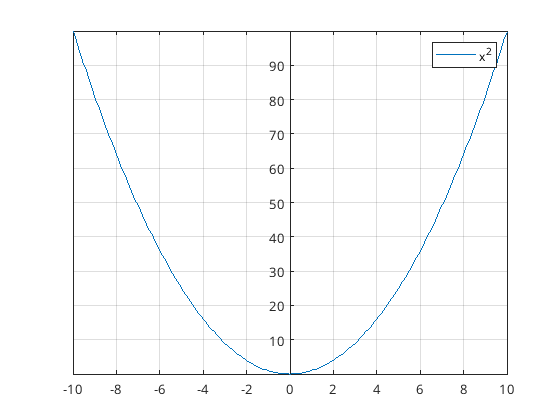
\includegraphics[width=0.5\textwidth]{immagini/Radix.png}
	\caption{\label{fig:SingleRadix}Grafico della radice della funzione $x^2$}
\end{figure}

\subsection{Metodo di bisezione}\footnote{PG. 19-22.}
Dato $[a,b]$, intervallo di confidenza per la radice $x^*$ di (\ref{eq:radice_equazione}) (aumentandone così la
precisione), è scelto in tale intervallo un punto in modo tale che questo sia la migliore approssimazione della radice. Il punto scelto è 
\begin{equation*}
	x^*\approx x_1=\frac{a+b}{2},
\end{equation*}
ovvero è selezionato il punto medio dell'intervallo.

Solo uno dei tre seguenti casi può verificarsi:
\begin{enumerate}
	\item $f(x_1)=0$, la soluzione è determinata ($x_1=x^*$);
	\item $f(a)f(x_1)<0$, il procedimento descritto può essere ripetuto sull'intervallo $[a, x_1]$ ($x^*\in[a, x_1]$);
	\item $f(x_1)f(b)<0$, il procedimento descritto può essere ripetuto sull'intervallo $[x_1, b]$ ($x^*\in[x_1, b]$).
\end{enumerate}

\begin{remark}
	È possibile osservare che nei casi 2. e 3. l'ampiezza dell'intervallo di confidenza si dimezza ad ogni passo perché sostituito, ad ogni passo, l'estremo opportuno.
\end{remark}

\begin{remark}
	Dati $[a_1,b_1]\equiv [a,b],\, x_1=\frac{a_1+b_1}{2}\Rightarrow x_n=\frac{a_n+b_n}{2}$, dove $x_n$ è l'approssimazione di $x^*$. Ulteriori chiarimenti sono forniti nella Sezione \ref{sec:critArresto}.
\end{remark}

È possibile che esistano più radici per la funzione $f$, un metodo iterativo come quello di bisezione ne approssima solamente una (vedere Figura \ref{fig:sinx}).


\begin{example}
	Sia $p(x)=(x-1.1)^{20}(x-\pi)$, in Matlab $p(\pi)\approx 10^{-5}$. È possibile, in altri termini, ottenere il seguente risultato:
	\begin{lstlisting}[style=Matlab-editor]
		p = poly([1.1*ones(1,20) pi]);
		polyval(p,pi);
		ans = -5.521324170132402e-05
	\end{lstlisting}
\end{example}

\paragraph{Implementazione del metodo di bisezione:} Vedere Algoritmo \ref{alg:metodo_bisezione}.

\begin{figure}
	\centering
	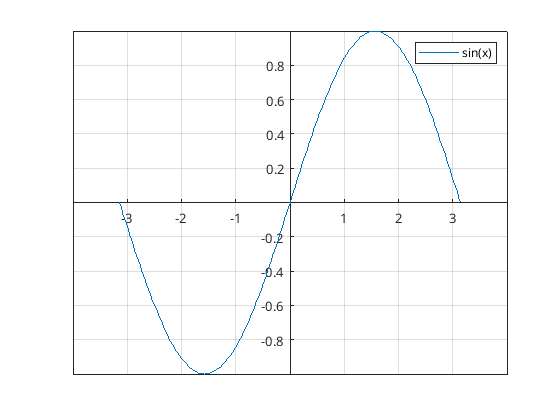
\includegraphics[width=0.5\textwidth]{immagini/tripleRadix.png}
	\caption{\label{fig:sinx}Grafico della funzione $\sin{(x)}$ (radici multiple)}
\end{figure}

\subsection{Criterio di Arresto}\label{sec:critArresto}
Quando è possibile fermare la successione di approssimazioni $x_n$? Un possibile criterio d'arresto può essere $f(x_n)=0$. Questa condizione è improbabile che si verifichi, è inutilizzabile, perché è possibile arrivare alla radice $x^*$ solo quando $x^*=x_n$, quindi in un numero infinito di passi. Questo non è compatibile con un elaboratore in aritmetica finita, dove $f(x^*)=f(x_n)\neq 0$, a causa dell'aritmetica finita stessa.

Realisticamente è possibile richiedere che 
\begin{equation}\label{eq:x_n_leq_tolx}
	|x_n-x^*|\leq \boldsymbol{tolx},
\end{equation}
dove $\boldsymbol{tolx}$ è noto, in quanto scelto dall'utente e rappresenta il massimo errore (assoluto) che sarà commesso. Questa disuguaglianza è utile al fine di determinare se esiste un numero finito di iterazioni che permetta un livello di tolleranza dell'errore accettabile ($\boldsymbol{tolx}$).

\subsubsection{Criterio di arresto per il metodo di bisezione} Dato un intervallo di confidenza iniziale $[a,b]\equiv [a_1,b_1]$ e l'approssimazione iniziale $x_1=\frac{(a_1+b_1)}{2}$, allora, al passo $i-$esimo, sarà ottenuto l'intervallo di confidenza $[a_i,b_i]$ e l'approssimazione $x_i=\frac{(a_i+b_i)}{2}$. Al passo $n-$esimo sarà ottenuto l'intervallo di confidenza $[a_n,b_n]$ e l'approssimazione $x_n=\frac{(a_n+b_n)}{2}$.

\paragraph{In quanti passi è approssimata la radice $\boldsymbol{x^*}$?}
Per il metodo di bisezione è possibile affermare che
\begin{equation*}
	\begin{matrix}
		\text{Numero iterazione} & \text{Errore} & \text{Intervallo di confidenza}\\\\
		1 & |x_1-x^*| \leq \frac{b-a}{2} & [a,b] \\\\
		2 & |x_2-x^*|\leq \frac{x_1-a}{2}=\frac{b-a}{4}  & [a_2,b_2]\\\\
		\vdots & \vdots & \vdots \\\\
		i & |x_i-x^*|\leq\frac{b-a}{2^i} & [a_i,b_i]\\\\
		\vdots & \vdots & \vdots \\\\
		n & |x_n-x^*|\leq\frac{b-a}{2^n} & [a_n,b_n]
	\end{matrix}
\end{equation*}
dove $\boldsymbol{\frac{b-a}{2^i}}$ è \textbf{stima dell'errore} al passo $i$-esimo.

L'obbiettivo è determinare $n$ in modo tale $|x_n-x^*|\leq tolx$. Fermandosi all'iterazione $n$ allora 
\begin{equation*}
	|x_n-x^*|\leq\frac{b-a}{2^n}\leq tolx,
\end{equation*}
è soddisfatto $\frac{b-a}{2^n}\leq tolx$ e quindi:
\begin{equation*}
	\begin{matrix}
		&& |x_n-x^*| &\leq& \boldsymbol{tolx}\\
		&\overset{\footnotemark}{\Rightarrow}&\frac{b-a}{2^n}&\leq& tolx \\
		&\Rightarrow& 2^n&\leq&\frac{b-a}{tolx}\\
		&\Rightarrow& \boldsymbol n &\boldsymbol\geq&\left\lceil \log_{2}\left(\frac{b-a}{tolx}\right)\right\rceil&\overset{\footnotemark}{=}&\boldsymbol{\lceil \log_{2}(b-a)-\log_{2}(tolx)\rceil}&\boldsymbol\equiv& \boldsymbol{itmax}.
	\end{matrix}
\end{equation*}

\addtocounter{footnote}{-1}
\footnotetext{$n$ è scelto in modo tale che si verichi ciò che segue.}

\stepcounter{footnote}
\footnotetext{$\lceil\, \rceil$ significa arrotondamento all'intero successivo.}

\begin{definition}[Numero massimo di iterazioni (metodo bisezione)]\label{def:itmax_metodo_bisezione}
	Dato l'insieme $[a,b]$, il numero massimo di iterazioni per verificare la conzione (\ref{eq:x_n_leq_tolx}) con il metodo di bisezione è
	\begin{equation*}
		\boldsymbol{\lceil \log_{2}(b-a)-\log_{2}(tolx)\rceil \equiv itmax}
	\end{equation*}
\end{definition}

\paragraph{È possibile soddisfare $\boldsymbol{|x_n-x^*|\leq tolx}$ con meno di $\boldsymbol{itmax}$ passi:}
È possibile, per effettuare meno di $itmax$, approssimare $|x_i-x^*|$ come segue:
\footnote{Ricordando che di $f$ è ricercata la radice ovvero $x^*:f(x^*)=0$, allora è possibile quanto segue.}
\begin{equation*}
	\begin{matrix}
		f(x)&\overset{\footnotemark}{\equiv}& f(x^*)+f'(x^*)(x-x^*)&=&f'(x^*)(x-x^*)\\
		&\overset{\footnotemark}{\Rightarrow}&f(x_i)&\approx& f'(x^*)(x_i-x^*)
	\end{matrix}
\end{equation*}
\footnotemark  allora
\begin{equation*}
	\boldsymbol{|x_i-x^*| \approx \frac{|f(x_i)|}{|f'(x^*)|}},
\end{equation*}
quindi
\begin{equation*}
	\boldsymbol{|x_n-x^*| \approx \frac{|f(x_n)|}{|f'(x^*)|}},
\end{equation*}

\addtocounter{footnote}{-2}
\footnotetext{Sviluppo di Taylor.}

\stepcounter{footnote}
\footnotetext{È ricercata $f(x_i)$, ovvero è effettuata la sostituzione $x=x_i$.}

\stepcounter{footnote}
\footnotetext{Essendo $|x_i-x^*|$ la quantità ricercata allora la conseguenza è logica.}

\noindent e pertanto \textbf{è possibile utilizzare} $\boldsymbol{\frac{|f(x_i)|}{|f'(x^*)|}}(\leq tolx)$ \textbf{come criterio d'arresto} ($i=1,\hdots, n$). 

Al fine di utilizzare $f'(x^*)$ nel criterio di arresto, questa può essere approssimata, dato l'intervallo di confidenza $[a_i, b_i]$, come segue:
\begin{equation}\label{eq:approxf'}
	\boldsymbol{f'(x^*)\approx\frac{f(b_i)-f(a_i)}{b_i-a_i}=\frac{f(a_i+\overbrace{b_i-a_i}^{h})-f(a_i)}{\underbrace{b_i-a_i}_{h}}\rightarrow \lim_{i\to + \infty}\frac{f(b_i)-f(a_i)}{b_i-a_i}}.
\end{equation}

\begin{remark}[Non ufficiale]
	Il costo computazionale dell'approssimazione $f'(x^*)$ calcolata come (\ref{eq:approxf'}) è nullo perché $f(a_i)$ e $f(b_i)$ sono già calcolati nel metodo di bisezione.\\
	Inoltre,
	\begin{equation*}
		\frac{|f(x_i)|}{|f'(x^*)|}\leq tolx \iff |f(x_i)|\leq \boldsymbol{|f'(x^*)|\cdot tolx=tolf}(\rightarrow |f(x_i)|\leq tolf),
	\end{equation*}
	con ${tolf}$ quantità precisa [\footnotemark]. In altre parole: per avere $|x_n-x^*|\leq tolx$ occorre utilizzare una tolleranza $tolf\approx|f'(x^*)|\cdot tolx$.
	\footnotetext{Se $tolf>>1$ (vedi Figura \ref{fig:f1(xStar)major1.jpg}), significa che $x_i$ è vicino a $x^*$ e ciò è un buon indicatore per determinare l'affidabilità legata all'errore.}
\end{remark}

\begin{figure}
	\centering
	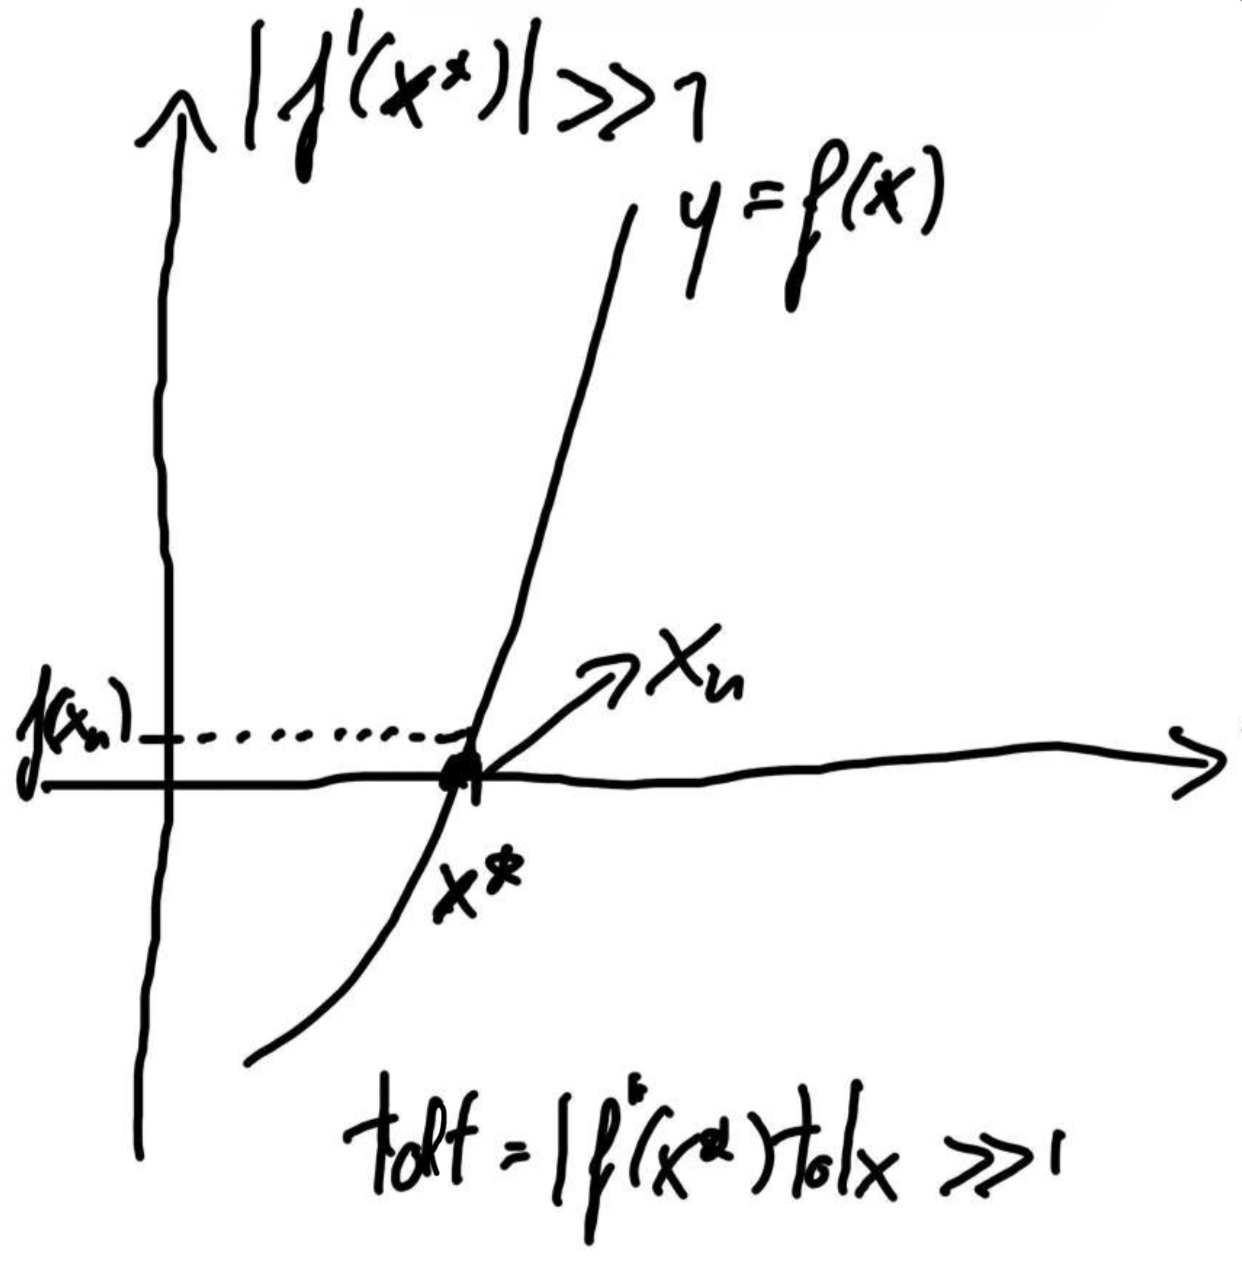
\includegraphics[width=0.5\textwidth]{immagini/f1(xStar)major1.jpg}
	\caption{\label{fig:f1(xStar)major1.jpg}$f'(x^*)>>1$}
\end{figure}
\begin{figure}
	\centering
	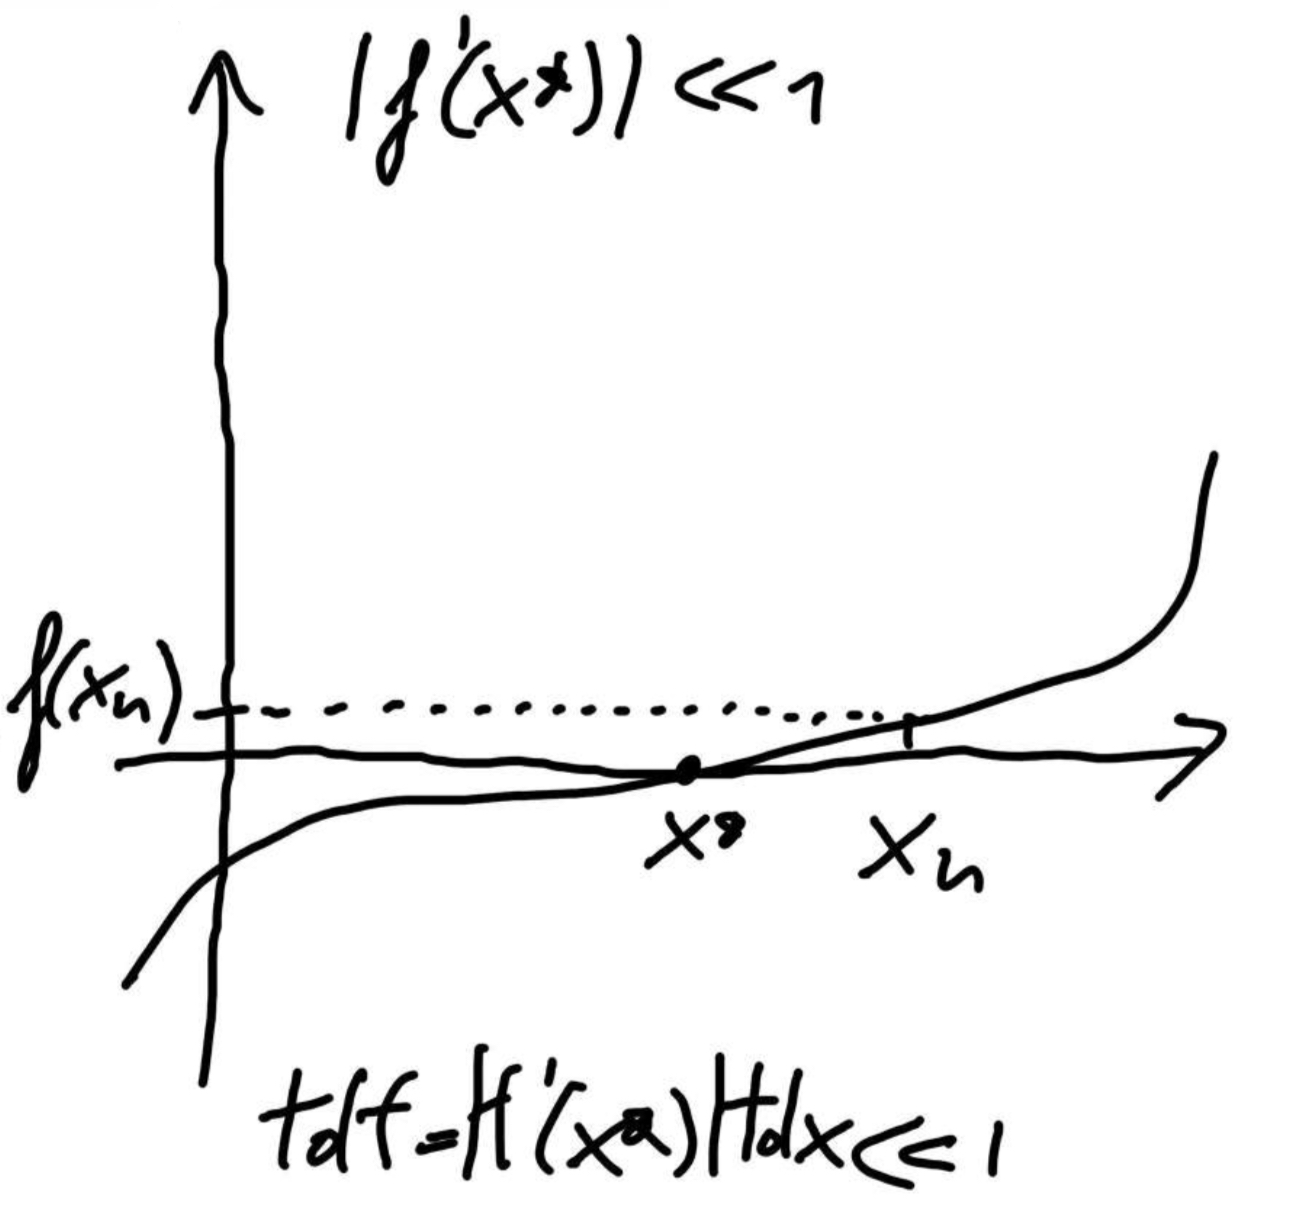
\includegraphics[width=0.5\textwidth]{immagini/f1(xStar)minor1.jpg}
	\caption{\label{fig:f1(xStar)minor1.jpg} $f'(x^*)<<1$}
\end{figure}

\subsubsection{Condizionamento di una radice}\footnote{PG 23, slide 6 PDF lez7.} L'analisi appena condotta per definire un criterio d'arresto più efficiente per il metodo di bisezione è legata al condizionamento della radice $x^*$ e rimarrà valida anche per i metodi che saranno trattati successivamente.

\begin{definition}[Numero di condizionamento di una radice]\label{def:numero_condizionamento_radice}
	Sia $f$ ed $x^*$ la radice trovata. Il numero di condizionamento della radice $x^*$ è dato da
	\begin{equation}\label{eq:defK}
		\boldsymbol{\kappa =\frac{1}{|f'(x^*)|}.}
	\end{equation}
\end{definition}
Tale valore amplifica (di un fattore $\kappa$) l'errore $|x_i-x^*|$ commesso su $x^*$.

\begin{remark}[Non ufficiale]
	Data $tolf = |f'(x*)|tolx$, è possibile osservare che:
	\begin{itemize}
		\item se $|f'(x^*)|\approx 0\Rightarrow tolf\ll tolx\; \left(\frac{1}{|f'(x^*)|}\gg 1\right)$, $x^*$ è una radice malcondizionata;
		
		\item se $|f'(x^*)|\geq 1 \Rightarrow tolf\gg tolx\; \left(\frac{1}{|f'(x^*)|}\leq 1\right)$, $x^*$ è una radice bencondizionata.
	\end{itemize}
\end{remark}

\begin{example}[Condizionamento radice di un polinomio]\footnote{PG 25.}
	Nel caso del polinomio $p(x)=(x-1.1)^{20}(x-\pi)$ è ottenuta $p'(\pi)=(\pi-1.1)^{20}\approx 1.6\cdot 10^6$. Il numero di condizionamento vale $\kappa\approx 6\cdot 10^{-7}$ e quindi la radice $x^*=\pi$ è ben condizionata.
\end{example}

\begin{definition}[Errore della radice]
	L'errore (perturbazione) sul risultato (di approssimazione della radice) può essere approssimato come
	\begin{equation*}
		|x_n-x^*|\approx\frac{|f(x_n)|}{|f'(x^*)|}=\underbrace{\frac{1}{|f'(x^*)|}}{\kappa}|f(x_n)|,
	\end{equation*}
	dove:
	\begin{itemize}
		\item $|f(x_n)|$ è la perturbazione rispetto al valore esatto $|f(x^*)|=0$,
		\item  $\frac{1}{|f'(x^*)|}$ il condizionamento della radice.
	\end{itemize}
\end{definition}

\paragraph{N.B.:} È necessario osservare che il condizionamento riguarda il problema e non il \gls{metodo numerico}.

\begin{definition}[Radice con molteplicità $m$]\label{def:radice_molteplicita_m}
	\footnote{PG 25, slide 7 PDF lez 7.} $x^*$ è una radice del problema (\ref{eq:radice_equazione}) ed ha molteplicità esatta $m\geq 1$, se è verificato quanto segue:
	\begin{equation*}
		f(x^*)=f'(x^*)=f''(x^*)=\hdots=f^{(m-1)}(x^*)=0,\, f^{(m)}(x^*)\neq 0.
	\end{equation*}
\end{definition}
Se $m=1$ allora $x^*$ si dice radice semplice, altrimenti (per $m\geq 2$) si dice multipla.

\paragraph{Il metodo di bisezione è malcondizionato con radici multiple:} Dalla Definizione precedente e dalla Definizione \ref{def:numero_condizionamento_radice} di condizionamento di una radice è possibile affermare che il problema della determinazione di radici multiple è \textbf{\underline{sempre} malcondizionato} \uline{per ogni metodo impiegato per la ricerca delle radici}. Quindi  il numero di condizionamentodei metodi utilizzati risulta essere $\kappa=\infty$ ed il risultato, la radice, sarà impreciso. Il malcondizionamento del problema ha precise ripercussioni sulla velocità di convergenza verso la radice di tutti i metodi introdotti.

\paragraph{Convergenza del metodo di bisezione:} Vedere Sezione \ref{ssec:convergenza_metodo_bisezione}.

\begin{algorithm}\caption{Implementazione ottimale del metodo di bisezione.}
	\label{alg:metodo_bisezione}
	\begin{lstlisting}[style=Matlab-editor]
		function x = bisezione(f, a, b) % da applicare controllo f(a)f(b)<0 (Teorema degli zeri)
		fa = feval(f, a);
		fb = feval(f, b);
		imax = ceil(log2(b-a) - log2(tolx));
		for i =  1 : imax
		x = (a + b)/2;
		fx = feval(f,x);
		f1x = abs((fb - fa)/(b - a));
		if abs(fx) <= tolx * f1x
		break
		elseif fa * fx < 0
		b = x;
		fb = fx;
		else
		a = x;
		fa = fx;
		end
		end
		return
	\end{lstlisting}
\end{algorithm}

\subsection{Ordine di convergenza di un metodo iterativo}\footnote{PG 26-28, slide 8-9 + 1-2 PDF lez7-8.} Lo scopo dell'argomento introdotto è quello di misurare l'errore di approssimazione della radice, quindi che il metodo iterativo sia corretto nel funzionamento. Ciò che sarà stabilito è la convergenza della successione alla radice.
\begin{definition}[Errore di approssimazione]
	Supposto di voler risolvere l'equazione (\ref{eq:radice_equazione}) e sia $x_i$ l'approssimazione fornita al passo $i-$esimo, è possibile definire l'errore di approssimazione come
	\begin{equation}\label{eq:errore_metodo_iterativo}
		e_i:=x_i-x^*.
	\end{equation}
\end{definition} 

\begin{definition}[Metodo iterativo convergente]
	Un metodo iterativo è convergente s.se \begin{equation}\label{eq:limite_errore_metodo_convergente}
		\lim_{i\to+\infty}{e_i}=0.
	\end{equation}
\end{definition}

Il passo successivo alla definizione di convergenza è quello di stabilire la velocità computazionale del metodo (quanto velocemente $x_n$ si avvicina a $x^*$? Quanti calcoli servono?). Per questo è necessaria l'introduzione di \textbf{Definizione \ref{def:ordine_convergenza_metodo_iterativo}} di ordine di convergenza e \textbf{Osservazione \ref{rem:limite_ordine_convergenza}.}
\begin{definition}[\textbf{Ordine di convergenza} di un metodo iterativo] \label{def:ordine_convergenza_metodo_iterativo}
	Se un metodo iterativo ha $p\in\mathbb R^+$ come valore più grande per cui
	 \begin{equation}\label{eq:limite_ordine_convergenza}
		\lim_{i\to + \infty}{\frac{|e_{i+1}|}{|e_i|^p}}=c<\infty,
	\end{equation}
	allora tale metodo ha \textbf{ordine di convergenza} $\boldsymbol p$, con \textbf{costante asintotica dell'errore} $\boldsymbol c$.
\end{definition}

\begin{remark}
	Se $e_i<1 \Rightarrow |e_i|^p$ è sempre più piccolo al crescere di $p$.
\end{remark}

Nel caso in cui $p=1$ si parla di convergenza lineare, con $p = 2$ di convergenza quadratica, eccetera. \textbf{Nonostante $\boldsymbol p$ possa assumere non intero e minore di 1, è necessario che $\boldsymbol{p \geq 1}$ affinché sia convergente.}

\begin{remark}\label{rem:limite_ordine_convergenza}
	Per $i$ sufficientemente grande, nel caso di convergenza lineare ($p=1$), è ottenuto (data (\ref{eq:limite_ordine_convergenza})):
	\begin{equation*}
		\frac{|e_{i+1}|}{|e_i|^p}\approx c,
	\end{equation*}
	allora
	\begin{equation}\label{eq:approssimazione_errore_i+1}
		|e_{i+1}|\approx c|e_i|^p.
	\end{equation}
\end{remark}

\begin{remark}\label{rem:metodo_lineare_convergente}
	Un \textbf{\gls{metodo lineare}} ($p=1$) è \textbf{convergente s.se} $\boldsymbol{0\leq c<1}$.
\end{remark}

\paragraph{Perché l'Osservazione \ref{rem:metodo_lineare_convergente} vale?} Dato (\ref{eq:approssimazione_errore_i+1}) allora, se $p=1$
\begin{equation*}
	|e_{i+1}|\approx c|e_i|\Rightarrow |e_{i+k}|\approx c^k|e_{i-k}|\Rightarrow |e_i|\approx c^i|e_0|,
\end{equation*}
quindi
\begin{equation*}
	\underset{i\to\infty}{\lim}|e_i|=\underset{i\to\infty}{\lim}{c^i|e_0|}\iff c<1.
\end{equation*}

Più è elevato l'ordine di un metodo convergente, più le approssimazioni generate dal metodo convergono verso la radice $x^*$. Questo è accentuato nel prossimo esempio.

\begin{example}
	\footnote{PG 27, slide 1 PDF lez8.} Considerati 2 metodi iterativi convergenti alla stessa radice $x^*$, con ordine di convergenza rispettivamente $p=1$ e $p=2$, entrambi con costante $c=0.1$, se per entrambi $e_0=0.1$, allora
	\begin{center}
		\begin{tabular}{ |c|c|c|c| } 
			\hline
			$i$ & $p=1$ & $p=2$ \\
			\hline
			0 & 0.1 & 0.1 \\ 
			1 & $c|e_0|^1=10^{-2}$ & $c|e_0|^2=10^{-3}$ \\ 
			2 & $c|e_1|^1=10^{-3}$ & $c|e_1|^2=10^{-7}$\\
			3 & $c|e_2|^1=10^{-4}$ & $c|e_2|^2=10^{-15}$\\
			4 & $c|e_3|^1=10^{-5}$ & $c|e_3|^2=10^{-31}$\\
			\hline
		\end{tabular}
	\end{center}
	
	È possibile osservare come la tabella sia ottenuta dall'applicazione della Definizione \ref{def:ordine_convergenza_metodo_iterativo} e che $e_i=c|e_{i-1}|^1,\, \forall i=1,\hdots , n$ (dove, nella tabella, $n=4$).
\end{example}

\subsubsection{Metodo di bisezione}\label{ssec:convergenza_metodo_bisezione}
\begin{remark}(Convergenza metodo di bisezione)
	Il metodo di bisezione è sempre convergente (convergenza globale): 
	\begin{equation*}
		|e_i|=|x_i-x^*|\leq \frac{b-a}{2^i}\Rightarrow \boldsymbol{0\leq \lim_{i\to + \infty}|e_i|\leq \lim_{i\to + \infty}{\frac{b-a}{2^i}=0}\Rightarrow \lim_{i\to + \infty}{e_i}=0.}
	\end{equation*}
\end{remark}

\noindent Inoltre, \textbf{il metodo di bisezione ha ordine di convergenza assimilabile a $\boldsymbol{p=1}$ e costante asintotica dell'errore $\boldsymbol{c=\frac{1}{2}}$}, ovvero \textbf{converge linearmente} \footnotemark. Questo è dovuto a $\underset{{i\to\infty}}{\lim}{\frac{|e_{i+1}|}{|e_i|}}=\frac{1}{2}$, utilizzando la stima assegnata al metodo di bisezione $|e_i|\leq\frac{b-a}{2^i}$.

\footnotetext{Quindi il metodo di bisezione converge $R-$linearmente (informazione non richiesta).}

\subsection{Metodo di Newton}\label{ssec:metodo_newton}
\footnote{Slide 3-8, 1-2 PDF 8,11 PDF 9,10.}
Il metodo di Newton è un metodo di approssimazione della radice con ordine migliore del metodo di bisezione. Questo metodo iterativo si basa su un'approssimazione lineare della funzione a partire dalla soluzione approssimata corrente, ovvero: supposto di conoscere un'approssimazione $y$ della funzione, allora il sistema generale per determinare $x^*$ tale che $f(x^*)=0$ è
\begin{equation*}
	\begin{cases}
		y = f(x),\\
		y = 0,
	\end{cases}
\end{equation*}
dal quale, attraverso l'utilizzo della retta tangente al grafico di $f$ nel punto $(x_0,f(x_0))$
\begin{equation}\label{eq:retta_tangente_in_0}
	\begin{cases}
		y = f(x_0) + f'(x_0)(x-x_0), \\
		y = 0,
	\end{cases}
\end{equation}
è ricavata, tramite calcoli intermedi (\footnotemark), l'approssimazione (definita dall'approssimazione di tale retta con l'asse delle ascisse)
\begin{equation*}
	x_1=x_0-\frac{f(x_0)}{f'(x_0)},
\end{equation*}
la quale è definita per $f'(x_0)\neq 0$, con $x_0$ approssimazione iniziale di $x^*$. Reiterando per $i$ passi successivi, è possibile ottenere l'espressione funzionale del metodo di Newton:
\begin{equation}\label{eq:approssimazione_newton}
	x_{i+1}=x_i-\frac{f(x_i)}{f'(x_i)}, \quad i=0,1,2,\hdots
\end{equation}

\footnotetext{Da (\ref{eq:retta_tangente_in_0}) $y=0\Rightarrow\frac{f(x_0)}{f'(x_0)}+\cancel{f'(x_0)}(x-x_0)=0\Rightarrow x-x_0=-\frac{f(x_0)}{x_0}\Rightarrow x=x_0-\frac{f(x_0)}{x_0}.$}

\begin{figure}
	\centering
	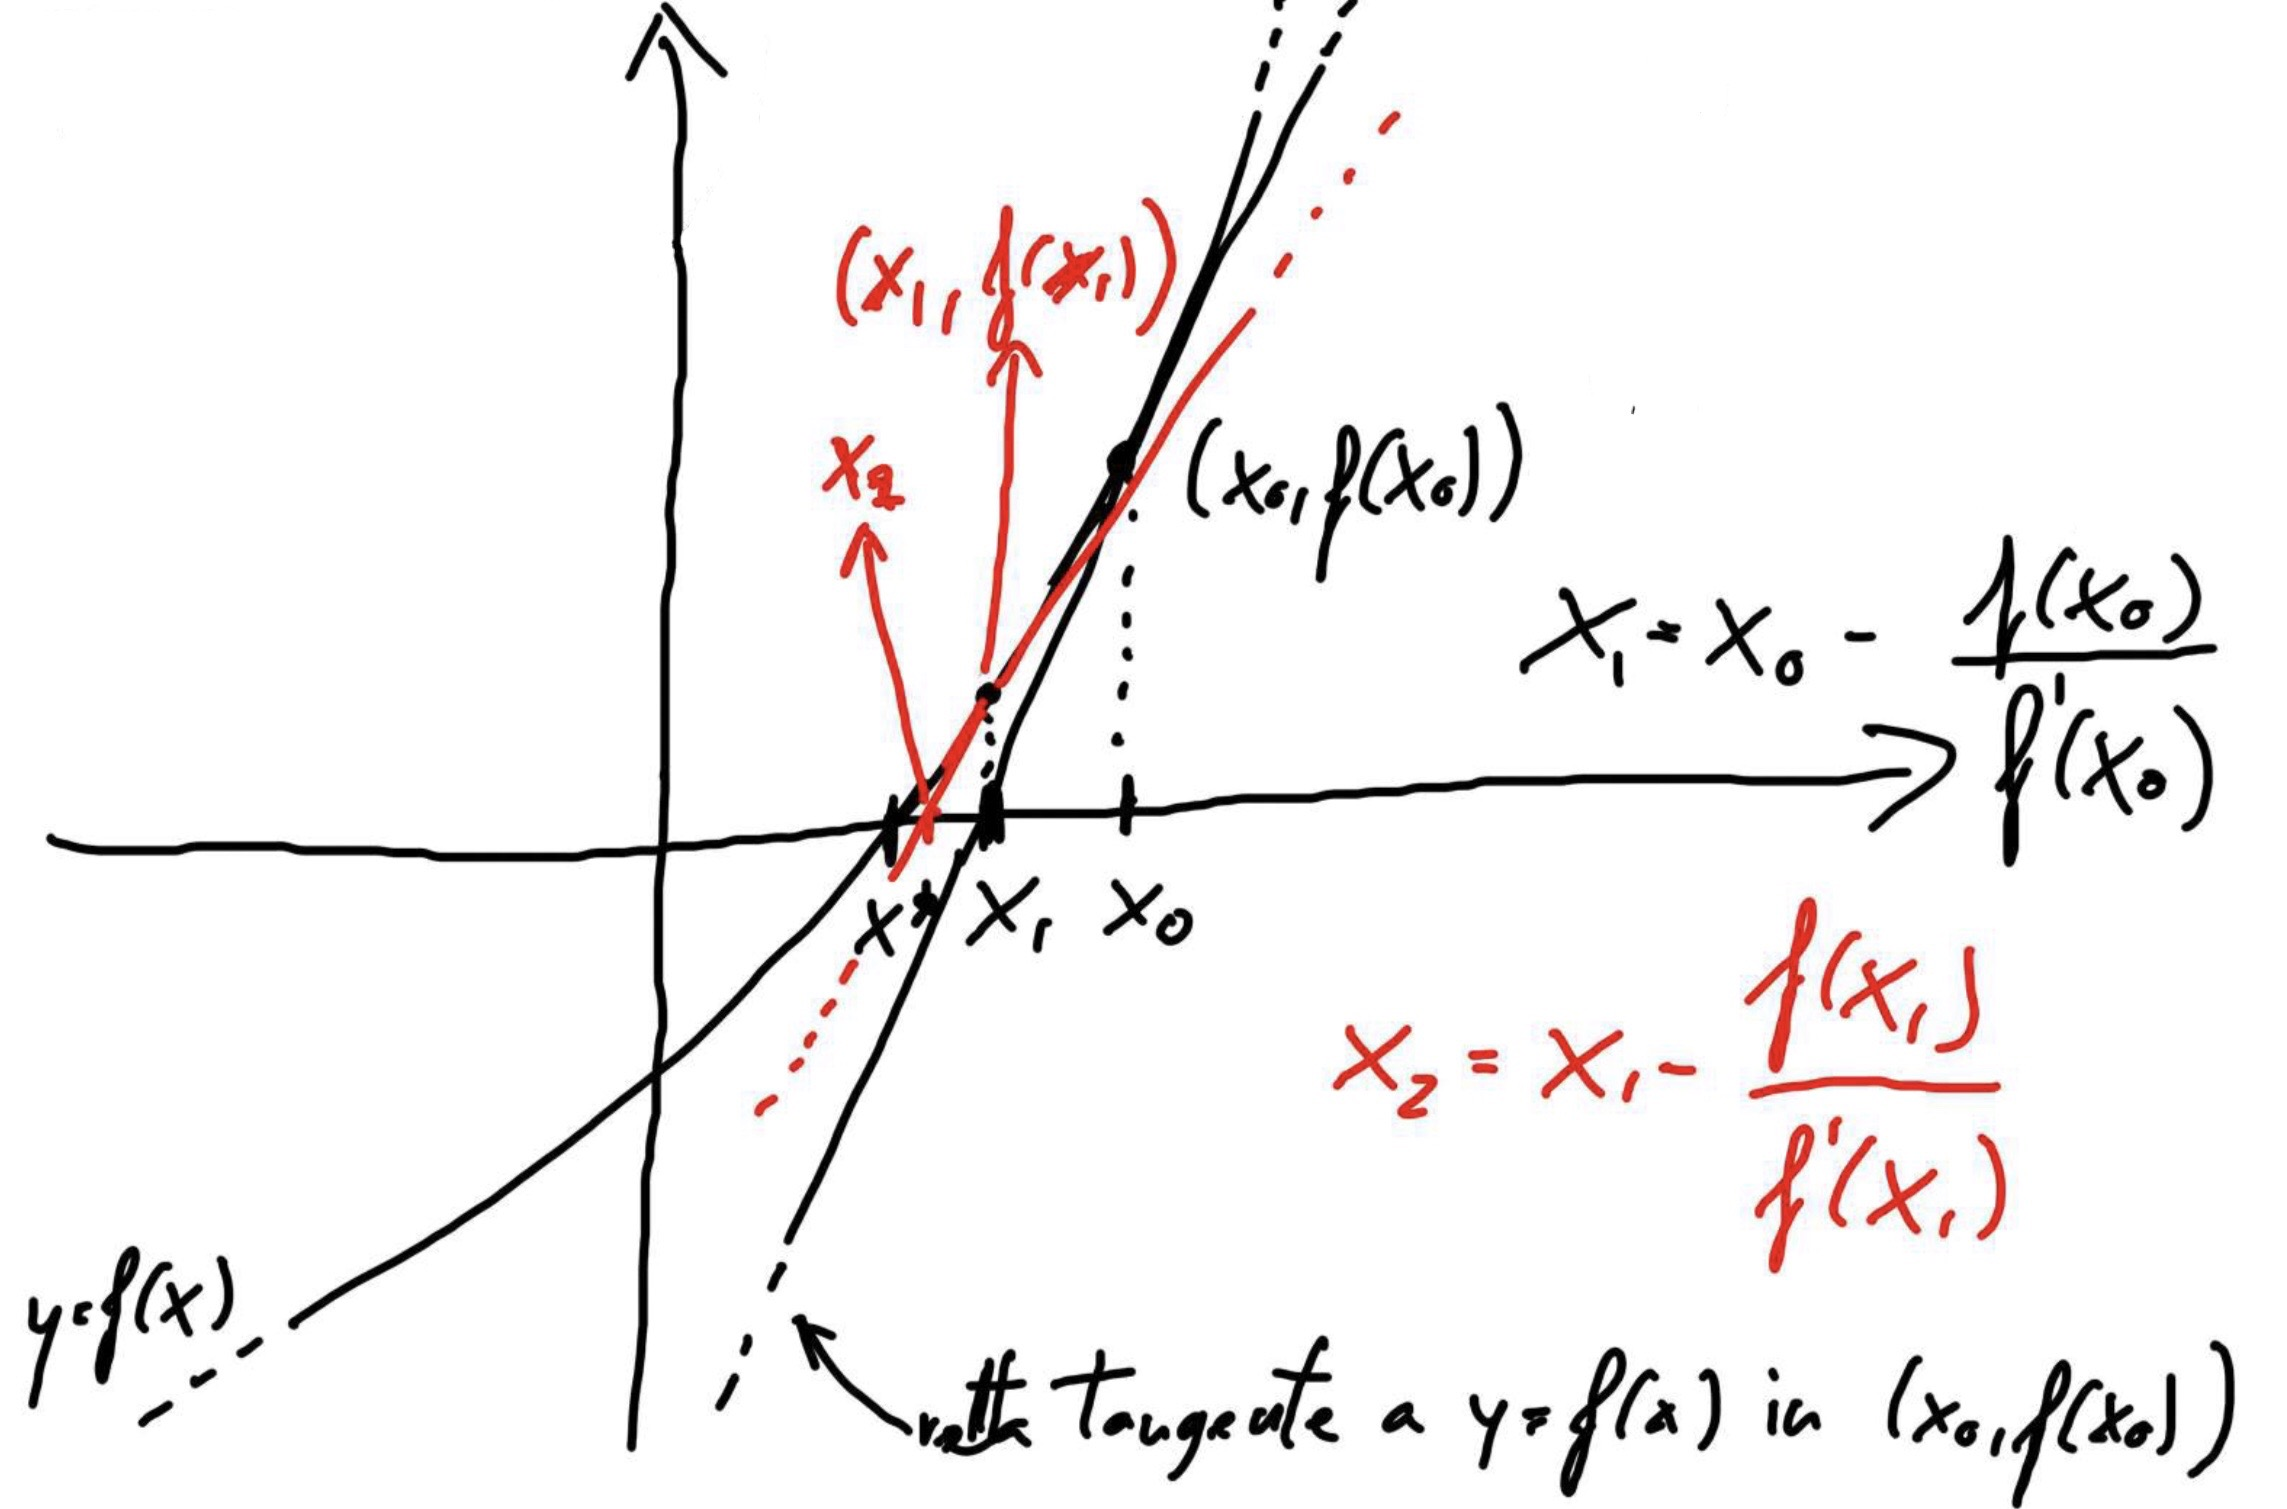
\includegraphics[width=0.5\textwidth]{immagini/GraficoRettaTangNewton.jpg}
	\label{fig:grafico_retta_tangente_metodo_newton}
	\caption{Grafico $y=f(x)$ con relative approssimazioni ottenute tramite Newton (è ricercata l'intersezione).}
\end{figure}

Più passi vengono calcolati, più $x_i$ si avvicina a $x^*$.

\paragraph{Osservazioni sul metodo:} La soluzione al problema (\ref{eq:radice_equazione}) è ottenuta risolvendo \gls{equazioni lineari}. Nel caso in cui $f(x)$ sia una \gls{funzione lineare} allora il metodo di Newton fornisce la soluzione in un solo passo.

\paragraph{Costo computazionale:}È possibile osservare che il metodo di Newton ha un costo per iterazione di 2 valutazioni funzionali (il metodo di bisezione ne richiede una): è necessario calcolare $f(x)$ ed $f'(x)$, in quanto ad ogni passo/iterazione cambia l'input ($x_0, x_1, x_2, \hdots$).
Inoltre, mentre il metodo di bisezione richiede solo la continuità della funzione $f$, per il metodo di Newton è richiesto che $f$ sia, oltre che continua, derivabile (ovvero $f\in C^{(2)}$).
Il costo computazionale maggiore e maggiori requisiti del metodo, rispetto al metodo di bisezione, sono compensati dall'elevato ordine di convergenza del metodo.

\begin{theorem}[\textbf{Metodo di Newton converge quadraticamente a radici semplici}, nome non ufficiale]\label{th:metodo_newton_converge_quadraticamente}
	Se $f(x)$ è sufficientemente regolare, \textbf{il metodo di Newton converge quadraticamente} (ovvero con ordine $p=2$) \textbf{verso radici semplici} \footnote{Ovvero radici di molteplicità 1, le quali sono definite come $x^*:f(x^*)=0,\, f'(x^*)\neq 0$.}.
\end{theorem}
\begin{proof}
	Assunto che $f\in C^{(2)}$ in un intorno della radice $x^*$, preso un opportuno $\xi_i$ (non noto) compreso fra $x^*$ e $x_i$, tramite lo sviluppo di Taylor di ordine 2 centrato in $x_i$
	\begin{equation*}
		f(x)=f(x_i)+f'(x_i)(x-x_i)+\frac{f''(\xi_i)}{2}(x-x_i)^2, \quad \xi_i \text{ compreso fra }x,x_i,
	\end{equation*}
	è valutata $f$ tramite lo sviluppo di Taylor centrato in $x^*$
	\begin{equation*}
		\begin{matrix}
			0 &=& f(x^*)\\
			&=& f(x_i)+f'(x_i)(x^*-x_i)+\frac{f''(\xi_i)}{2}(x^*-x_i)^2 \\
			&\overset{\footnotemark}{=}& f'(x_i)\left[\frac{f(x_i)}{f'(x_i)}-x_i+x^*\right]+\frac{f''(\xi_i)}{2}(x^*-x_i)^2 \\
			&\overset{\footnotemark}{=}&f'(x_i)(-x_{i+1}+x^*)+\frac{f''(\xi_i)}{2}(x^*-x_i)^2\\
			&\overset{\footnotemark}{=}&-f'(x_i)e_{i+1}+\frac{f''(\xi_i)}{2}e_i^2 &\rightarrow&\frac{f''(\xi_i)}{2}e_i^2 &=& -f'(x_i)e_{i+1}\\
			&&&\overset{\footnotemark}{\Rightarrow}& \frac{|e_{i+1}|}{|e_i^2|} &=& \frac{1}{2}\frac{|f''(\xi_i)|}{|f'(x_i)|}, && x^*<\xi_i<x_i.
		\end{matrix}
	\end{equation*}
	\addtocounter{footnote}{-3}
	\footnotetext{Raccolto $f'(x_i)$ perché interessante la q.tà $\frac{f(x_i)}{f'(x_i)}-x_i$ (ovvero $x_{i+1}$ cambiato di segno).}
	
	\stepcounter{footnote}
	\footnotetext{Sostiuzione di $\frac{f(x_i)}{f'(x_i)}-x_i$ con $-x_{i+1}$.}
	
	\stepcounter{footnote}
	\footnotetext{Sostituzione $x^*-x_{i+1}=-e_{i+1}$ e $x^*-x_i=-e_i$.}
	
	\stepcounter{footnote}
	\footnotetext{L'obbiettivo è valutare quanto segue.}
	
	\noindent Allora, supponendo che il metodo converga (ovvero che $\lim_{i\rightarrow+\infty}x_i=x^*$): 
	\begin{equation*}
		\lim_{i\to + \infty}{\frac{|e_{i+1}|}{|e_i|^2}}=\lim_{i\to + \infty}{\frac{1}{2}\frac{f''(\xi_i)}{f'(x_i)}}\overset{\footnotemark}{=}\frac{1}{2}\frac{f''\left(\underset{i\to\infty}{\lim}\xi_i\right)}{f'\left(\underset{i\to\infty}{\lim}{x_i}\right)}=\frac{1}{2}\frac{f''(x^*)}{f'(x^*)},
	\end{equation*}
	
	\footnotetext{$f\in C^{(2)}$, quindi $f''$ è continua.}
	
	\noindent quindi, per $f'(x^*)=0$ ($x^*$ radice semplice)\footnote{Ipotesi importante perché significa che $f'(x^*)\neq 0$ e che quindi $\frac{f''(x^*)}{f'(x^*)}\neq\infty$.}:
	\begin{equation*}
		\lim_{i\to + \infty}{\frac{|e_{i+1}|}{|e_i|^2}}=\frac{1}{2}\frac{f''(x^*)}{f'(x^*)}<\infty,
	\end{equation*}
	e \textbf{il metodo ha ordine di convergenza $\boldsymbol{p=2}$.}\footnote{L'ordine è almeno 3 se $f''(x^*)=0$.}
\end{proof}

\begin{theorem}[\textbf{Convergenza lineare di Newton}, nome non ufficiale]\label{th:convLineareNewt}
	\footnote{Teorema utilizzato per radici non semplici.}
	Se $f(x)$ è sufficientemente regolare in un intorno di $x^*$, radice di molteplicità $m>1$, \textbf{il metodo di Newton converge linearmente ($p=1$) verso una radice di molteplicità} $\boldsymbol{m>1}$, \textbf{con costante asintotica dell'errore $\boldsymbol{c=\frac{m-1}{m}}$}.
\end{theorem}
\begin{proof}\footnote{Slide 8, 1-2 PDF lez8, lez9.}
	Sia $x^*$ radice con molteplicità $m>1$, è possibile esprimere $f$ come $f(x)=(x-x^*)^mg(x)$, con $g$ funzione tale che $g(x^*)\neq 0$ e sviluppabile in serie di Taylor centrato in $x^*$. È possibile ottenere quanto segue, per $x_i\approx x^*$ (vedi (\ref{eq:errore_metodo_iterativo}), (\ref{eq:approssimazione_newton}) e l'Osservazione \ref{rem:formaF}): 
	\begin{equation*}
		\begin{matrix}
			\frac{e_{i+1}}{e_i}&=&\frac{x_{i+i}-x^*}{x_i-x^*}&\overset{\footnotemark}{=}&\frac{x_i-\frac{f(x_i)}{f'(x_i)}-x^*}{x_i-x^*}\\\\
			&\overset{\footnotemark}{=}&\frac{\cancel{x_i-x^*}-\frac{(x_i-x^*)^mg(x_i)}{m{(x_i-x^*)^{m-1}}g(x_i)+(x_i-x^*)^mg'(x_i)}}{\cancel{x_i-x^*}}&=&1-\frac{(x_i-x^*)^{m-1}g(x_i)}{m(x_i-x^*)^{m-1}g(x_i)+(x_i-x^*)^mg(x_i)}\\\\
			&=&\frac{m(\cancel{x_i-x^*)^{m-1}}g(x_i)+(x_i-x^*)^{\cancel{m}}g'(x_i)-\cancel{(x_i-x^*)^{m-1}}g(x_i)}{m\cancel{(x_i-x^*)^{m-1}}g(x_i)+\cancel{(x_i-x^*)^m}g'(x_i)}&\overset{\footnotemark}{=}&\frac{mg(x_i)+(x_i-x^*)g'(x_i)-g(x_i)}{mg(x_i)+(x_i-x^*)g'(x_i)}\\\\
			&\overset{\footnotemark}{=}&\frac{(m-1)g(x_i)+e_ig'(x_i)}{mg(x_i)+e_ig'(x_i)}&\overset{\footnotemark}{\Rightarrow}&\frac{e_{i+1}}{e_i}=\frac{(m-1)g(x_i)+e_ig'(x_i)}{mg(x_i)+e_ig'(x_i)}.
		\end{matrix}
	\end{equation*}
	
	\addtocounter{footnote}{-4}
	
	\footnotetext{Sostituzione di $x_{i+1}$ con $x_i-\frac{x_i}{f'(x_i)}$ per applicare la definizione del metodo di Newton.}
	
	\stepcounter{footnote}
	\footnotetext{Dato che $f(x)=(x-x^*)^mg(x)$ allora $f'(x)=m(x-x^*)^{m-1}g(x)+(x-x^*)^mg'(x)$.}
	
	\stepcounter{footnote}
	\footnotetext{Divisione di numeratore e denominatore per $(x_i-x)^{m-1}$.}
	
	\stepcounter{footnote}
	\footnotetext{Raccoglimento $g(x_i)$ e sostituzione di $(x_i-x^*)$ con $e_i$.}
	
	\stepcounter{footnote}
	\footnotetext{È dimostrato quanto segue.}
	
	\noindent Allora, dalla (\ref{eq:limite_errore_metodo_convergente}):
	\begin{equation} \label{eq:limCostanteAsistotica}
		\boldsymbol{\lim_{i\to + \infty}{\frac{|e_{i+1}|}{|e_i|}}}=\lim_{i\to + \infty}{\frac{|(m-1)\,g(x_i)+e_i\,g'(x_i)|}{|m\,g(x_i)+e_i\,g(x_i)|}}\overset{\footnotemark}{=}\lim_{i\to + \infty}{\frac{|(m-1)\,\cancel{g(x_i)}|}{|m\,\cancel{g(x_i)}|}}=\boldsymbol{\frac{m-1}{m}}.
	\end{equation}
	
	\footnotetext{È supposto che il problema di Newton converga quindi, per il fatto stesso di convergere (vedi (\ref{eq:limite_errore_metodo_convergente})), l'errore $(e_i)$ tende a 0, quindi $\underset{i\to\infty}{\lim}e_ig'(x_i)\to 0$.}
	
	\noindentÈ dimostrata così la tesi, ovvero: il metodo di Newton converge linearmente con costante asintotica $\frac{m-1}{m}$.
\end{proof}

\subsubsection{Convergenza del metodo di Newton}\footnote{Sul libro è "Convergenza Locale", slide 3-10, 1-3 PDF lez9, lez10 PG 30-33.} 
L'ordine di convergenza di un metodo convergente quantifica la "velocità" di avvicinamento delle approssimazioni alle radici. È necessario stabilire le condizioni che garantiscono la convergenza del metodo, ovvero che il metodo generi una successione di approssimazioni $\{x_i\}$ che soddisfi (\ref{eq:errore_metodo_iterativo})-(\ref{eq:limite_errore_metodo_convergente}).

Nel caso del metodo di bisezione, assumendo che $f\in C([a,b])$ t.c. $f(a)f(b)<0$, è possibile affermare che il metodo abbia proprietà di convergenza globale. Tale proprietà garantisce sempre la convergenza della serie di approssimazioni verso una radice di $f$. Purtroppo questa è pressoché proprietà esclusiva del metodo di bisezione.

Il metodo di Newton è convergente in un opportuno intorno della radice che dipende dalla scelta dell'approssimazione iniziale $x_0$.
\begin{example} [Controesempio di non convergenza]
	Data l'approssimazione $x_{i+1}=x_i-\frac{f(x_i)}{f'(x_i)}$, è applicato il metodo di Newton a $f(x)=x^3-5x$, con approssimazione iniziale $x_0=1$. Calcolata $f'$ di $f$ (prima cosa da calcolare), ovvero $f'(x)=3x^2-5$, è possibile il calcolo le seguenti approssimazioni:
	\begin{equation*}
		x_1=x_0-\frac{f(x_0)}{f'(x_0)}=1-\frac{1-5}{3-5}=-1;\quad x_2=x_1-\frac{f(x_1)}{f'(x_1)}=1-\frac{-1+5}{3-5}=1;\quad x_3=-1;\quad x_4=1,\quad\hdots,
	\end{equation*}
	allora la successione di approssimazioni ottenuta non converge ad alcuna radice (ed $x_0$ non è una radice).
\end{example}

\begin{figure}
	\centering
	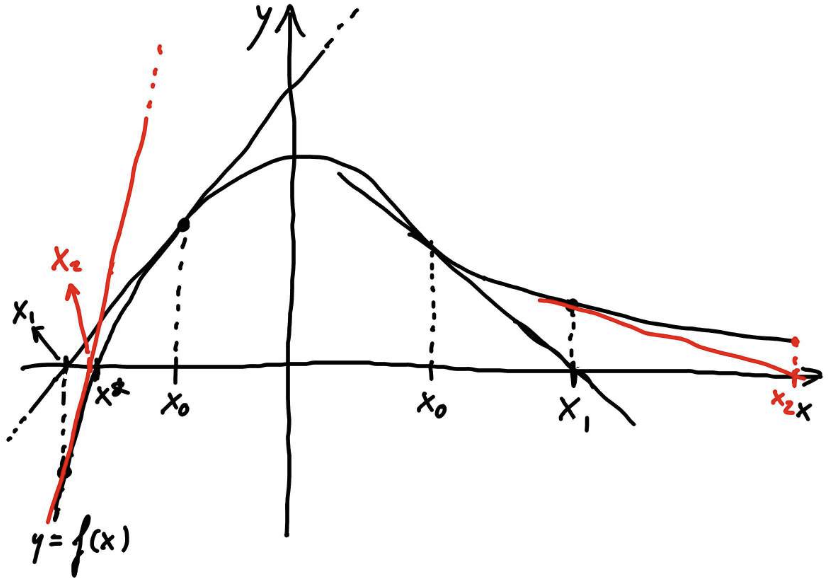
\includegraphics[width=0.75\textwidth]{immagini/EsemGeoConv.png}
	\caption{\label{fig:esempio_geometrico_convergenza}Esempio dal punto di vista geometrico della convergenza.}
\end{figure}

Tramite la Figura \ref{fig:esempio_geometrico_convergenza} è possibile osservare quanto segue: \begin{itemize}
	\item più le rette tangenti (le linee che toccano il grafico di $y=f(x)$) si avvicinano a $x^*$, più  il metodo converge ed è preciso;
	\item il problema di convergenza sorge se $x_0$ è scelto come nel primo quadrante perché i successivi calcoli ($x_1, x_2, \hdots$) si allontanano da $x^*$; quindi è necessario scegliere $x_0$ nell'intervallo locale della radice in base alla funzione.
\end{itemize}

\subsubsection{Studio della convergenza locale}
Questa Sezione è una formalizzazione della Figura \ref{fig:esempio_geometrico_convergenza}.
Lo studio della convergenza locale in un contesto generale può essere formalizzata come segue: considerato un metodo iterativo per l'approssimazione di una radice, l'approssimazione della radice $x^*$ di $f$, è definita da
\begin{equation}\label{eq:funzIteraz}
	x_{i+1}=\Phi (x_i)\quad i=0,1,2,\hdots,
\end{equation}
con $\Phi (x_i)$ funzione d'iterazione, la quale caratterizza il metodo di iterazione generico \footnote{Tale funzione è una regola che fornisce una buona approssimazione applicando $\Phi$ a partire da $x_i$.}.

Affinché il metodo iterativo abbia senso, supposto che $x_i\rightarrow x^*$ per $i\rightarrow\infty$, è richiesto che $\boldsymbol{x^*}$ sia il \textbf{punto fisso} della funzione di iterazione $\boldsymbol{\Phi(x)}$, ovvero:
\begin{equation*}
	x^*=\Phi (x^*).
\end{equation*}

\begin{definition}[Funzione d'iterazione del metodo di Newton]
	Per il metodo di Newton la funzione di iterazione del metodo è
	\begin{equation}\label{eq:funzIterazNewton}
		\Phi (x)=x-\frac{f(x)}{f'(x)},
	\end{equation}
	quindi
	\begin{equation*}
		\Phi (x^*)=x^*-\frac{f(x^*)}{f'(x^*)}\overset{f(x^*)=0}{=}x^*.
	\end{equation*}
\end{definition}

Questo argomento permette di trattare le proprietà di convergenza del metodo iterativo, mediante lo studio delle proprietà di stabilità del punto fisso corrispondente della funzione di iterazione. La convergenza locale dei metodi può essere studiata mediante declinazioni del seguente teorema.

\begin{theorem}[\textbf{del punto fisso}]\label{th:puntofisso}
	\footnote{Slide 6 PDF lez9, PG 31-32.}
	Sia $\Phi(x)$ la funzione d'iterazione (\ref{eq:funzIteraz}) che definisce il \gls{metodo numerico}. Supposto che $\exists\,\delta >0,\; 0\leq L<1$, costanti tali che:
	\begin{equation*}
		|\Phi (x)-\Phi (y)|\leq L|x-y| \quad\forall x,y \in I=(x^*-\delta,\, x^*+\delta),
	\end{equation*}
	allora:
	\begin{enumerate}
		\item $x^*$ è l'unico punto fisso di $\Phi$ in $I$;
		\item se $x_0 \in I\Rightarrow x_{i+1} = \Phi(x_i)\in I,\quad i=0,1,2,\hdots$;
		\item se $x_0\in I \Rightarrow \underset{{i\to\infty}}{\lim}{x_i}=x^*$. (proprietà più interessante)
	\end{enumerate}
\end{theorem}

\begin{proof}
	La dimostrazione avverrà per punti:
	\begin{enumerate}
		\item Per assurdo (è supposto che esistano due punti fissi): $\exists\, x^*,\, \overline{x}\in I: \Phi(x^*)=x^*,\, \Phi(\overline{x})=\overline{x}$. Poichè $x \neq \overline{x}$, segue:
		\begin{equation*}
			|x^*-\overline{x}|=|\Phi(x^*)-\Phi(\overline{x})|\overset{\footnotemark}{\leq}L|x^*-\overline{x}|<|x^*-\overline{x}| \Rightarrow\text{ Assurdo } (|x^*-\overline{x}|\overset{\footnotemark}{\nless}|x^*-\overline{x}|).
		\end{equation*}
		Quindi il punto fisso in $I$ è unico (e tale punto è $x^*$);
		\addtocounter{footnote}{-1}
		\footnotetext{Applicazione del teorema.}
		\stepcounter{footnote}
		\footnotetext{$|x^*-\overline{x}|$ non può essere minore di se stesso.}
		\item Per induzione: dato $x_0 \in I = (x^*-\delta,\, x^* + \delta)$ è supposto che $x_i\in I \iff |x_i-x^*|<\delta$, quindi è possibile dimostrare che $x_i\in I$ come segue:
		\begin{equation*}
			|x_{i+1}-x^*|=|\Phi(x_i)-\Phi(x^*)|\overset{\footnotemark}{\leq}L|x_i - x^*| < L\,\delta\overset{\footnotemark}{<}\delta\Rightarrow |x_{i+1}-x^*|<\delta\Rightarrow x_{i+1}\in I;
		\end{equation*}
		\item È necessario dimostrare
		\begin{equation*}
			\lim_{i\to + \infty}{x_i}=x^*\iff \lim_{i\to + \infty}{|x_i-x^*|}=0.
		\end{equation*}
		Ciò che interessa calcolare è $|x_i-x^*|$, ovvero l'errore:
		\begin{equation*}
			\begin{matrix}
				|x_i-x^*|&\overset{\footnotemark}{=}&|\Phi(x_{i-1})-\Phi(x^*)|&\leq& L|x_{i-1}-x^*|&=& L|\Phi(x_{i-2})-\Phi(x^*)|\\
				&\leq& L\cdot L |x_{i-2}-x^*|&=& L^2|x_{i-2}-x^*|&\leq& \hdots &\leq& L^i|x_0-x^*|\\
				&\Rightarrow& |x_i-x^*|&\leq& L^i|x_0-x^*|.
			\end{matrix}
		\end{equation*}
		Quindi è possibile dimostrare la tesi come segue:
		\begin{equation*}
			0\leq \underbrace{\lim_{i \to\infty}{|x_i-x^*|}}_{\footnotemark}\leq\lim_{i\to + \infty}{L^i|x_0-x^*|}=0\Rightarrow \lim_{i\to + \infty}{|x_i-x^*|}=0\Rightarrow\lim_{i\to + \infty}{x_i=x^*}.
		\end{equation*}
	\end{enumerate}
\end{proof}

\addtocounter{footnote}{-4}
\footnotetext{Sfruttando le ipotesi del teorema.}

\stepcounter{footnote}
\footnotetext{$x_i,\, x^*\in I$.}

\stepcounter{footnote}
\footnotetext{$L<1$, quindi è valido ciò che segue.}

\stepcounter{footnote}
\footnotetext{$x_{i-1}, x^*\in I$ perché $x_0\in I$ e vale 2.}

\stepcounter{footnote}
\footnotetext{Limite calcolato con la disuguaglianza precedente.}

\noindent\footnote{Slide 1 PDF lez10, PG 32.} Inoltre, è possibile dimostrare che la funzione (\ref{eq:funzIterazNewton}) soddisfa le ipotesi del Teorema del punto fisso (Teorema \ref{th:puntofisso}), come segue: assumendo $f(x)\in C^{(2)}$ in un intorno di $x^*$, dove $x^*$ è la radice semplice di $f$ e definita $\Phi(x)\in C^{(1)}$ in un intorno di $x^*$ (come in (\ref{eq:funzIterazNewton})) con $\Phi'(x)=1-\frac{[f'(x)]^2-f(x)f''(x)}{[f'(x)]^2}$, allora
\begin{equation*}
	\Phi'(x^*)=1-\frac{[f'(x^*)]^2-f(x^*)f''(x^*)}{[f'(x^*)]^2}=1-\frac{[f'(x^*)]^2}{[f'(x^*)]^2}=1-1=0.
\end{equation*}
Quindi, $\Phi\in C^{(1)}\Rightarrow\Phi'\in C^{(0)}$ e $\Phi'(x^*)=0$.

Applicando la definizione di funzione continua\footnote{Definizione di funzione continua: $g$ è continua in $x^*$ s.se $\forall\varepsilon, \exists\,\delta>0:|g(x)-g(x^*)|<\varepsilon\quad\forall x\in I=(x^*-\delta,x^*+\delta)$.} a $\Phi=g$, $\varepsilon =L$ e fissato $0<L<1$:
\begin{equation*}
	\exists\,\delta>0:|\Phi'(x)-\Phi'(x^*)|<L \quad\forall x\in (x^*-\delta,x^*+\delta).
\end{equation*}


L'ipotesi è verificata con $L$ e $\delta$ scelte, utilizzando lo sviluppo di Taylor, in quanto
\begin{equation*}
	\begin{matrix}
		\forall x,y \in I=(x^*-\delta,\, x^*+\delta): |\Phi(x)-\Phi(y)| &\overset{\footnotemark}{=}& |\cancel{\Phi(x)}-\cancel{\Phi(x)}-\Phi'(\xi)(x-y)|  &\overset{\footnotemark}{=}& |\Phi'(\xi)(x-y)| \\
		&=& |\Phi'(\xi)||x-y| &<& L|x-y|\\
		&\Rightarrow&|\Phi(x)-\Phi(y)|&\leq& L|x-y|.
	\end{matrix}
\end{equation*}

\addtocounter{footnote}{-1}
\footnotetext{È necessario dimostrare che sia minore di $L|x-y|$. Inoltre, $\Phi(y)=\Phi(x)+\Phi(\xi)(x-y)$ con $\xi\in(x,y)\rightarrow\xi\in I$.}

\stepcounter{footnote}
\footnotetext{Approssimazione di $f(x)$ con sviluppo di Taylor.}

\begin{figure}
	\centering
	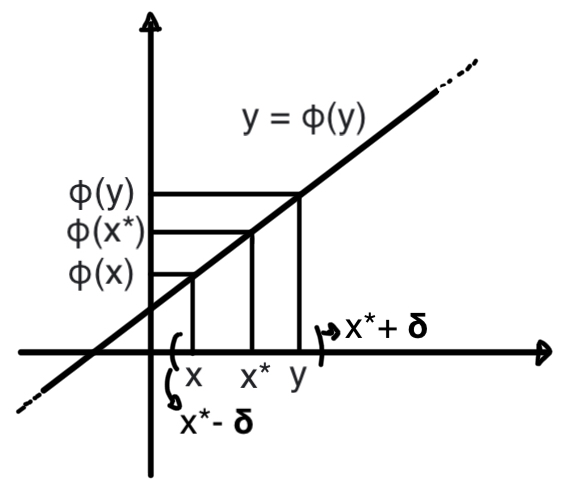
\includegraphics[width=0.5\textwidth]{immagini/TeoremaPuntoFisso.png}
	\caption{\label{fig:TeoremaPuntoFisso}Esempio del grafico di una funzione d'iterazione per il Teorema \ref{th:puntofisso}.}
\end{figure}

\subsubsection{Criteri d'arresto per il metodo di Newton (e non solo)}
\footnote{Slide 4 PDF lez10, PG 33.}
Gli argomenti trattati nella Sezione \ref{sec:critArresto}, riguardo la definizione di un criterio d'arresto basato sul controllo di $|f(x)|$ (ovvero $|f(x_i)|\leq|f'(x^*)|\, tolx$), sono applicati anche al caso del metodo di Newton (ed ai metodi quasi-Newton trattati in seguito). A causa della convergenza del metodo non è possibile determinare a priori il numero massimo di iterazioni entro le quali il criterio di accuratezza sulla approssimazione calcolata sarà soddisfatto. Dunque, in prossimità della radice $x^*$, nel caso di ordine di convergenza $p>1$,
\begin{equation}\label{eq:approxErroreNewton}
	|x_{i+1}-x_i|=|\underbrace{x_{i+1}-x^*}_{\text{$e_{i+1}$}}+\underbrace{x^*-x_i}_{\text{$e_{i}$}}|=|e_i-e_{i+1}|\overset{\footnotemark}{\approx}|e_i|.
\end{equation}
\footnotetext{$e_{i+1}\approx ce_i$. $\underset{i\to\infty}{\lim}\frac{|e_{i+1}|}{|e_i|^p}=c<\infty\Rightarrow |e_{i+1}|\approx c|e_i|^p\overset{p>1}{\Longrightarrow}e_{i+1}$ è trascurabile rispetto a $e_i$.}

Pertanto, un \textbf{criterio di arresto appropiato}, per metodi di \textbf{ordine di convergenza} $\boldsymbol{p>1}$ è del tipo
\begin{equation}\label{eq:critArrConvMag1}
	\boldsymbol{|x_{i+1}-x_i|\leq tolx}.
\end{equation}

Questo è dovuto al fatto che l'errore $|x^*-x_i|$ non è noto, quindi è necessario stimarlo, come in precedenza.

\begin{remark}[Criterio d'arresto per il metodo di Newton]
	Risulta essere sempre applicabile il seguente criterio d'arresto
	\begin{equation}\label{eq:critArrNewt}
		\boldsymbol{|f(x_i)|\leq |f'(x_i)|\cdot tolx}\equiv \frac{|f(x_i)|}{|f'(x_i)|}\leq tolx,
	\end{equation}
	il quale è ottenuto dalla Sezione \ref{sec:critArresto} tramite la disuguaglianza (\ref{eq:x_n_leq_tolx}) ($tolx$ ha lo stesso significato che ha in (\ref{eq:x_n_leq_tolx}
	)) .
\end{remark}

\begin{remark}[Criterio d'arresto ideale per il metodo di Newton]\footnote{Osservazione 2.3 PG 33, Slide 5 PDF lez10.}
	Oltre alla tolleranza sul massimo errore assoluto, $tolx$, è possibile utilizzare la tolleranza sull'errore relativo, $rtolx$ (o sull'accuratezza dell'approssimazione dello zero). In questo caso il controllo di arresto "ideale" diviene
	\begin{equation*}
		\frac{e_i}{tolx+rtolx|x^*|}\leq 1
	\end{equation*}
	e mediante le approssimazioni $x^*\approx x_{i+1}$ e $|e_i|\approx |x_{i+1}-x_i|$ il criterio da considerare è
	\begin{equation}\label{eq:critArrIdea}
		\boldsymbol{\frac{|x_{i+1}-x_i|}{tolx+rtolx|x_{i+1}|}\leq 1}.
	\end{equation}
	dove la disuguaglianza $e_i\leq tolx+rtolx|x^*|$ può essere rappresentata come
	\begin{equation*}
		\boldsymbol{\frac{1}{2}|e_i|\leq tolx} \wedge \frac{1}{2}|e_i|\leq rtolx|x^*| \iff \boldsymbol{\frac{1}{2}\frac{|e_i|}{x^*}\leq rtolx}
	\end{equation*}
	permettono di dividere in due il controllo (mediante ciò che è in grassetto). È spesso considerata la scelta $rtolx=tolx$, trasformando il criterio d'arresto (\ref{eq:critArrIdea}) in
	\begin{equation*}
		\frac{|x_{i+1}-x_i|}{1+|x_{i+1}|}\leq tolx.
	\end{equation*}
\end{remark}

Nel caso in cui la convergenza sia lineare (ovvero l'ordine di convergenza è $p=1$), il criterio d'arresto (\ref{eq:critArrConvMag1}) può essere modificato nel seguente (come \ref{eq:critArrIdea}), date (\ref{eq:limite_errore_metodo_convergente})-(\ref{eq:limite_ordine_convergenza}) e (\ref{eq:limCostanteAsistotica})):

\begin{equation}\label{eq:approxErroreNewtonBis}
	|x_{i+1}-x_i|=|e_{i+1}-e_i|=|e_i-\underbrace{e_{i+1}}_\text{$c\cdot e_i$}|\approx |e_i|(1-c)\Rightarrow |e_i|\approx\frac{|x_{i+1}-x_i|}{\underset{\footnotemark}{(1-c)}}.
\end{equation}
\footnotetext{Senza valore assoluto perché, per definizione di convergenza, i metodi convergenti hanno costante asintotica $c$ minore di 1.}

Se $c$ non è nota (nel caso del metodo di bisezione è $c=\frac{1}{2}$), è possibile, tramite (\ref{eq:approxErroreNewtonBis}), la seguente stima della costante asintotica c:
\begin{equation*}
	\boldsymbol{\frac{|x_{i+1}-x_i|}{|x_i-x_{i-1}|}\approx}\frac{\cancel{|e_{i-1}|}\,c\,\cancel{(1-c)}}{\cancel{|e_{i-1}|}\cancel{(1-c)}}=\boldsymbol c,
\end{equation*}
la quale è ottenuta tramite $i$ iterazioni del tipo
\begin{equation*}
	\begin{matrix}
		i=0 &:& |x_1-x_0|&\approx& |e_0|(1-c);\\
		i=1 &:& |x_2-x_1|&\approx&|e_i|(1-c)&\overset{\footnotemark}{\approx}&|e_0|\, c\, (1-c);\\
		\vdots & & \vdots & & \vdots \\
		i &:&|x_i-x_{i-1}|&\approx& |e_{i-1}|(1-c);\\
		i+1 &:&|x_{i+1}-x_i|&\approx& |e_i|(1-c) &=& |e_{i-1}|\, c\, (1-c);
	\end{matrix}
\end{equation*}
per renderla più precisa. Tale stima è utile per avere una buona  approssimazione dell'errore. Pertanto, è necessario considerare il costo computazionale delle $i$ iterazioni (sono necessarie almeno due iterazioni).
\footnotetext{$e_{i+1}\approx c\cdot e_i$.}

\subsection{Caso delle radici multiple}
\footnote{Slide 1-3 PDF lez11, PG 34-36.}
Per tutti i metodi per la ricerca delle radici di una funzione è noto che nel caso in cui la molteplicità di $x^*$ sia $m>1$, il problema di determinare le radici è malcondizionato in quanto $f'(x^*) = 0$ e quindi $\kappa = \frac{1}{|f'(x^*)|}=+\infty$. Questo è dovuto dalla definizione di molteplicità di una radice, ovvero dalla Definizione \ref{def:radice_molteplicita_m}, per la quale le prime $m$ derivate di $f$ sono tutte uguali 0.

Inoltre, è noto che il metodo di Newton risulti essere solo lineare. Tuttavia, è possibile modificare tale metodo per ripristinare la convergenza quadratica, distinguendo i seguenti casi.

\subsubsection{Molteplicità \texorpdfstring{$\boldsymbol{m>1}$}{m>1} nota}
Avere $m$ nota non è una caratteristica banale. Applicando l'Osservazione \ref{rem:formaF}, per semplicità, al metodo di Newton, per determinare la radice (\ref{eq:approssimazione_newton}), allora, è ottenuta
\begin{equation*}
	x_{i+1}=x_i-\frac{x_i-x^*}{m}, \quad i=0,1,2,\hdots.
\end{equation*}
Pertanto, il metodo di Newton è modificato come segue:
\begin{equation}\label{eq:approxNewtonMod}
	x_{i+1}=x_i-m\frac{f(x_i)}{f'(x_i)}, \quad i=0,1,2,\hdots,
\end{equation}
ripristinando la convergenza quadratica del metodo, qualora converga verso una radice di molteplicità esatta $m$.

\paragraph{Nota:} Saranno presenti riferimenti a questo paragrafo ed a (\ref{eq:approxNewtonMod}) come metodo di Newton modificato.

\paragraph{Convergenza:} Nel caso generale la \textbf{convergenza} rimane \textbf{quadratica}.

\subsubsection{Molteplicità \texorpdfstring{$\boldsymbol{m>1}$}{m>1} ignota}
In questo caso il metodo di Newton converge linearmente ($p=1$), quindi (da (\ref{eq:limite_ordine_convergenza}))
\begin{equation*}
	\underset{i\to\infty}{\lim}{\frac{|e_{i+1}|}{|e_i|}} = c<\infty.
\end{equation*}

Allora, per $i$ sufficientemente grande:
\begin{equation*}
	\begin{matrix}
		\boldsymbol{\frac{|e_{i+1}|}{e_i}\approx c}&\Rightarrow&
		\begin{matrix}
			e_i &\approx& c\cdot e_{i-1}\\
			e_{i+1}&\approx& c\cdot e_i
		\end{matrix}\\
		&\Rightarrow& e_i &\approx& \frac{e_{i+1}}{c}\\
		&\overset{\footnotemark}{\Rightarrow}& e_i^2&=&e_i\,e_i&\approx&\cancel{c}\cdot e_{i-1}\cdot \frac{e_{i+1}}{\cancel{c}}&=&e_{i-1}\cdot e_{i+1}\\
		&\boldsymbol\Rightarrow&\boldsymbol{e_i^2}&\boldsymbol\approx& \boldsymbol{e_{i-1}\cdot e_{i+1}}.
	\end{matrix}
\end{equation*}
\footnotetext{Dalle due relazioni (approssimazioni) è possibile ottenere ciò che segue.}

È possibile riscrivere la precedente approssimazione, l'ultima implicazione, come
\begin{center}
	$\underbrace{(x_i-x^*)^2}_{\text{$e_i^2$}}\approx\underbrace{(x_{i-1}-x^*)}_{\text{$e_{i-1}$}}\underbrace{(x_{i+1}-x^*)}_{\text{$e_{i+1}$}}$ 
\end{center}
e da questa segue che
\begin{equation*}
	\begin{matrix}
		x_i^2-2x_i x^*+\cancel{(x^*)^2}&\approx& x_{i-1} x_{i+1}-x_{i-1} x^* - x_{i+1} x^*+\cancel{(x^*)^2}\\
		&\rightarrow&-2x_i x^*+x_{i-1} x^*+x_{i+1}x^*&\approx&-x_i^2+x_{i-1} x_{i+1}\\
		&\rightarrow&(-2x_i+x_{i-1}+x_{i+1})x^* &\approx& -x_i^2+x_{i-1} x_{i+1}.
	\end{matrix}
\end{equation*}

Da quest'ultima approssimazione è possibile la seguente approssimazione della radice:
\begin{equation}\label{eq:approxAitken}
	x^*\approx x_i^*\equiv\frac{x_i^2-x_{i-1}\cdot x_{i+1}}{2x_i-x_{i-1}-x_{i+1}},
\end{equation}
dove $x_i^*$ rappresenta l'approssimazione di $x^*$ al passo $i-$esimo.

\begin{algorithm}
	\caption{Implementazione efficiente del metodo di Newton.}\label{alg:polNewt}
	\begin{lstlisting}[style=Matlab-editor]
		function x = newton(f, f1, x0, tol, itmax)
		%   
		%   x = newton(f, f1, x0, tol, itmax)
		%
		%   Metodo di Newton per la ricerca della radice di una funzione
		%
		% Input:
		%   f   -   function che implementa f(x);
		%   f1  -   function che implementa f'(x);
		%   x0  -   punto iniziale:
		%   tol -   tolleranza richiesta (default 1e-12);
		%   itmax   - numero massimo di iterazioni (default 1000);
		% Output:
		%   x   -   soluzione approssimata.
		%
		% Dalla riga successuva fino a x = x0 sono controlli strutturali.
		if nargin < 5
		itmax=1000;
		else
		if itmax < 1, error('itmax errato'); end
		end
		if nargin < 4 
		tol = 1e-12;
		else
		if tol < 0, error('tolleranza negativa'); end
		tol = max(tol, 10*eps);
		end
		if nargin < 3,  error('numero argomenti di ingresso errato'); end
		x = x0;
		for i = 1 : itmax
		xold = x;
		fx = feval(f,x);
		f1x = feval(f1, x);
		if f1x == 0, error('il metodo non converge'); end
		x = x - fx/f1x;
		err = abs(x-xold);
		if err <= tol, break; end
		end
		if err > tol, warning('tolleranza richiesta non soddifatta'), end
		return
	\end{lstlisting}
\end{algorithm}

\subsection{Metodo di Aitken}
\footnote{Slide 4-5 PDF lez11, PG 36-37.}
Il metodo utilizza una procedura a due livelli:
\begin{enumerate}
	\item Vengono eseguiti due passi del metodo di Newton (\ref{eq:approssimazione_newton}): 
	\begin{itemize}
		\item $x_{i-1}=x_{i-1}^*$;
		\item $x_i=x_{i-1}-\frac{f(x_{i-1})}{f'(x_{i-1})}$;
		\item $x_{i+1}=x_i-\frac{f(x_i)}{f'(x_i)}$;
	\end{itemize}
	\item Passo di Aitken: esecuzione del passo (\ref{eq:approxAitken}) di accelerazione, approssimare al meglio la radice. Questo passo fornirà il nuovo punto iniziale per il livello interno.
\end{enumerate}
La successione $\{x_i^*\}_{i=1,2,\hdots}$ generata con Aitken \underline{converge quadraticamente} verso $x^*$.
\paragraph{Costo computazionale} Pertanto, il prezzo di avere un'iterazione a due livelli è pagato con un costo computazionale doppio rispetto al classico Newton, ad ogni iterazione è applicato Newton due volte (per le quali sono necessarie le valutazioni di $f$ e $f'$).

\begin{algorithm}
	\caption{Implementazione metodo di Aitken.}\label{alg:metAit}
	\begin{lstlisting}[style=Matlab-editor]
		function x = aitken(f, f1, x, tolx, itmax)
		x = x0;
		for i = 1 : itmax
		x0 = x;
		fx = feval(f, x0);
		f1x = feval(f1, x0);
		x1 = x0 - fx/f1x;
		fx = feval(f, x1);
		f1x = feval(f1, x1);
		x = x1 - fx/f1x;
		x = (x*x0 - x1^2)/(x - 2*x1 + x0);
		if abs(x-x0) <= tolx, break, end
		end
		if abs(x-x0) > tolx, warning('il metodo non converge'), end
	\end{lstlisting}
\end{algorithm}

\subsection{Metodi quasi-Newton}
\footnote{Slide 6-10 PDF 11, PG 37-40.}
È possibile ridurre il costo di ogni iterazione del tipo (\ref{eq:approssimazione_newton}) attraverso un'approssimazione di $f'(x_i)$. I metodi in questa Sezione, variazioni del metodo di Newton, calcolano $x_{i+1}$ come segue:
\begin{equation}\label{eq:approssimazione_quasi_newton}
	x_{i+1}=x_i-\frac{f(x_i)}{\varphi_i}, \quad i=0,1,2,\hdots, \quad\varphi_i\approx f'(x_i).
\end{equation}

\subsubsection{Metodo delle corde}\label{sssec:metodo_corde}
È assunto che $f(x)$ sia sufficientemente regolare ed è presupposto che la derivata vari di poco in prossimità della radice.
Pertanto, se $x_0$ è vicino alla radice, allora è possibile approssimare $f'$ come
\begin{equation*}
	f'(x_i)\approx f'(x_0)\equiv\varphi_i,\; i=0,1,2,\hdots.
\end{equation*}
In questo modo è ottenuta l'iterazione 
\begin{equation}\label{eq:approxCorde}
	x_{i+1}=x_i-\frac{f(x_i)}{f'(x_0)}, \quad i=0,1,2,\hdots,
\end{equation}
la quale definisce il metodo delle corde.

È necessario notare che l'approssimazione della derivata sia una costante (ovvero $f'(x_0)$).

\paragraph{Costo computazionale:}\footnote{Il costo computazionale è considerato per iterazione.} 1 valutazione funzionale ($f(x_i)$).
\paragraph{Covergenza:}Si, locale.
\paragraph{Ordine di convergenza:} È lineare ($p = 1$) qualsiasi sia la molteplicità della radice.

Il metodo è utilizzato per la risoluzione di sistemi lineari per il basso costo di computazionale.

\subsubsection{Metodo delle secanti}\label{sssec:metodo_secanti}
\footnote{Slide 7-10 PDF lez11.}
Supposto siano già calcolati $x_{i-1}$ ed $x_i$, allora $f(x)\approx f(x_i)+(x-x_i)f'(x_i)$. La derivata può essere approssimata come 
\begin{equation*}
	f'(x_i)\approx\frac{f(x)-f(x_{i})}{x-x_i}\overset{x=x_{i-1}}{\Longrightarrow}f'(x_i)\approx\frac{f(x_i)-f(x_{i-1})}{x_i-x_{i-1}}\equiv\varphi_i.
\end{equation*}

L'iterazione (\ref{eq:approssimazione_quasi_newton}) diviene
\begin{equation}\label{eq:approxSecanti}
	\boldsymbol{x_{i+1}=x_i-\frac{f(x_i)(x_i-x_{i-1})}{f(x_i)-f(x_{i-1})}}=\frac{f(x_i)\,x_{i-1} - f(x_{i-1})\,x_i}{f(x_i)-f(x_{i-1})}, \quad i=1,2,\hdots,
\end{equation}
con $x_0$ ed $x_1$ approssimazioni iniziali assegnate (sono richiesti per il calcolo di $x_2$). Assegnato $x_0$ è possibile calcolare $x_1$, tramite il metodo di Newton, come $x_1=x_0-\frac{f(x_0)}{f'(x_0)}$.

\begin{figure}
	\centering
	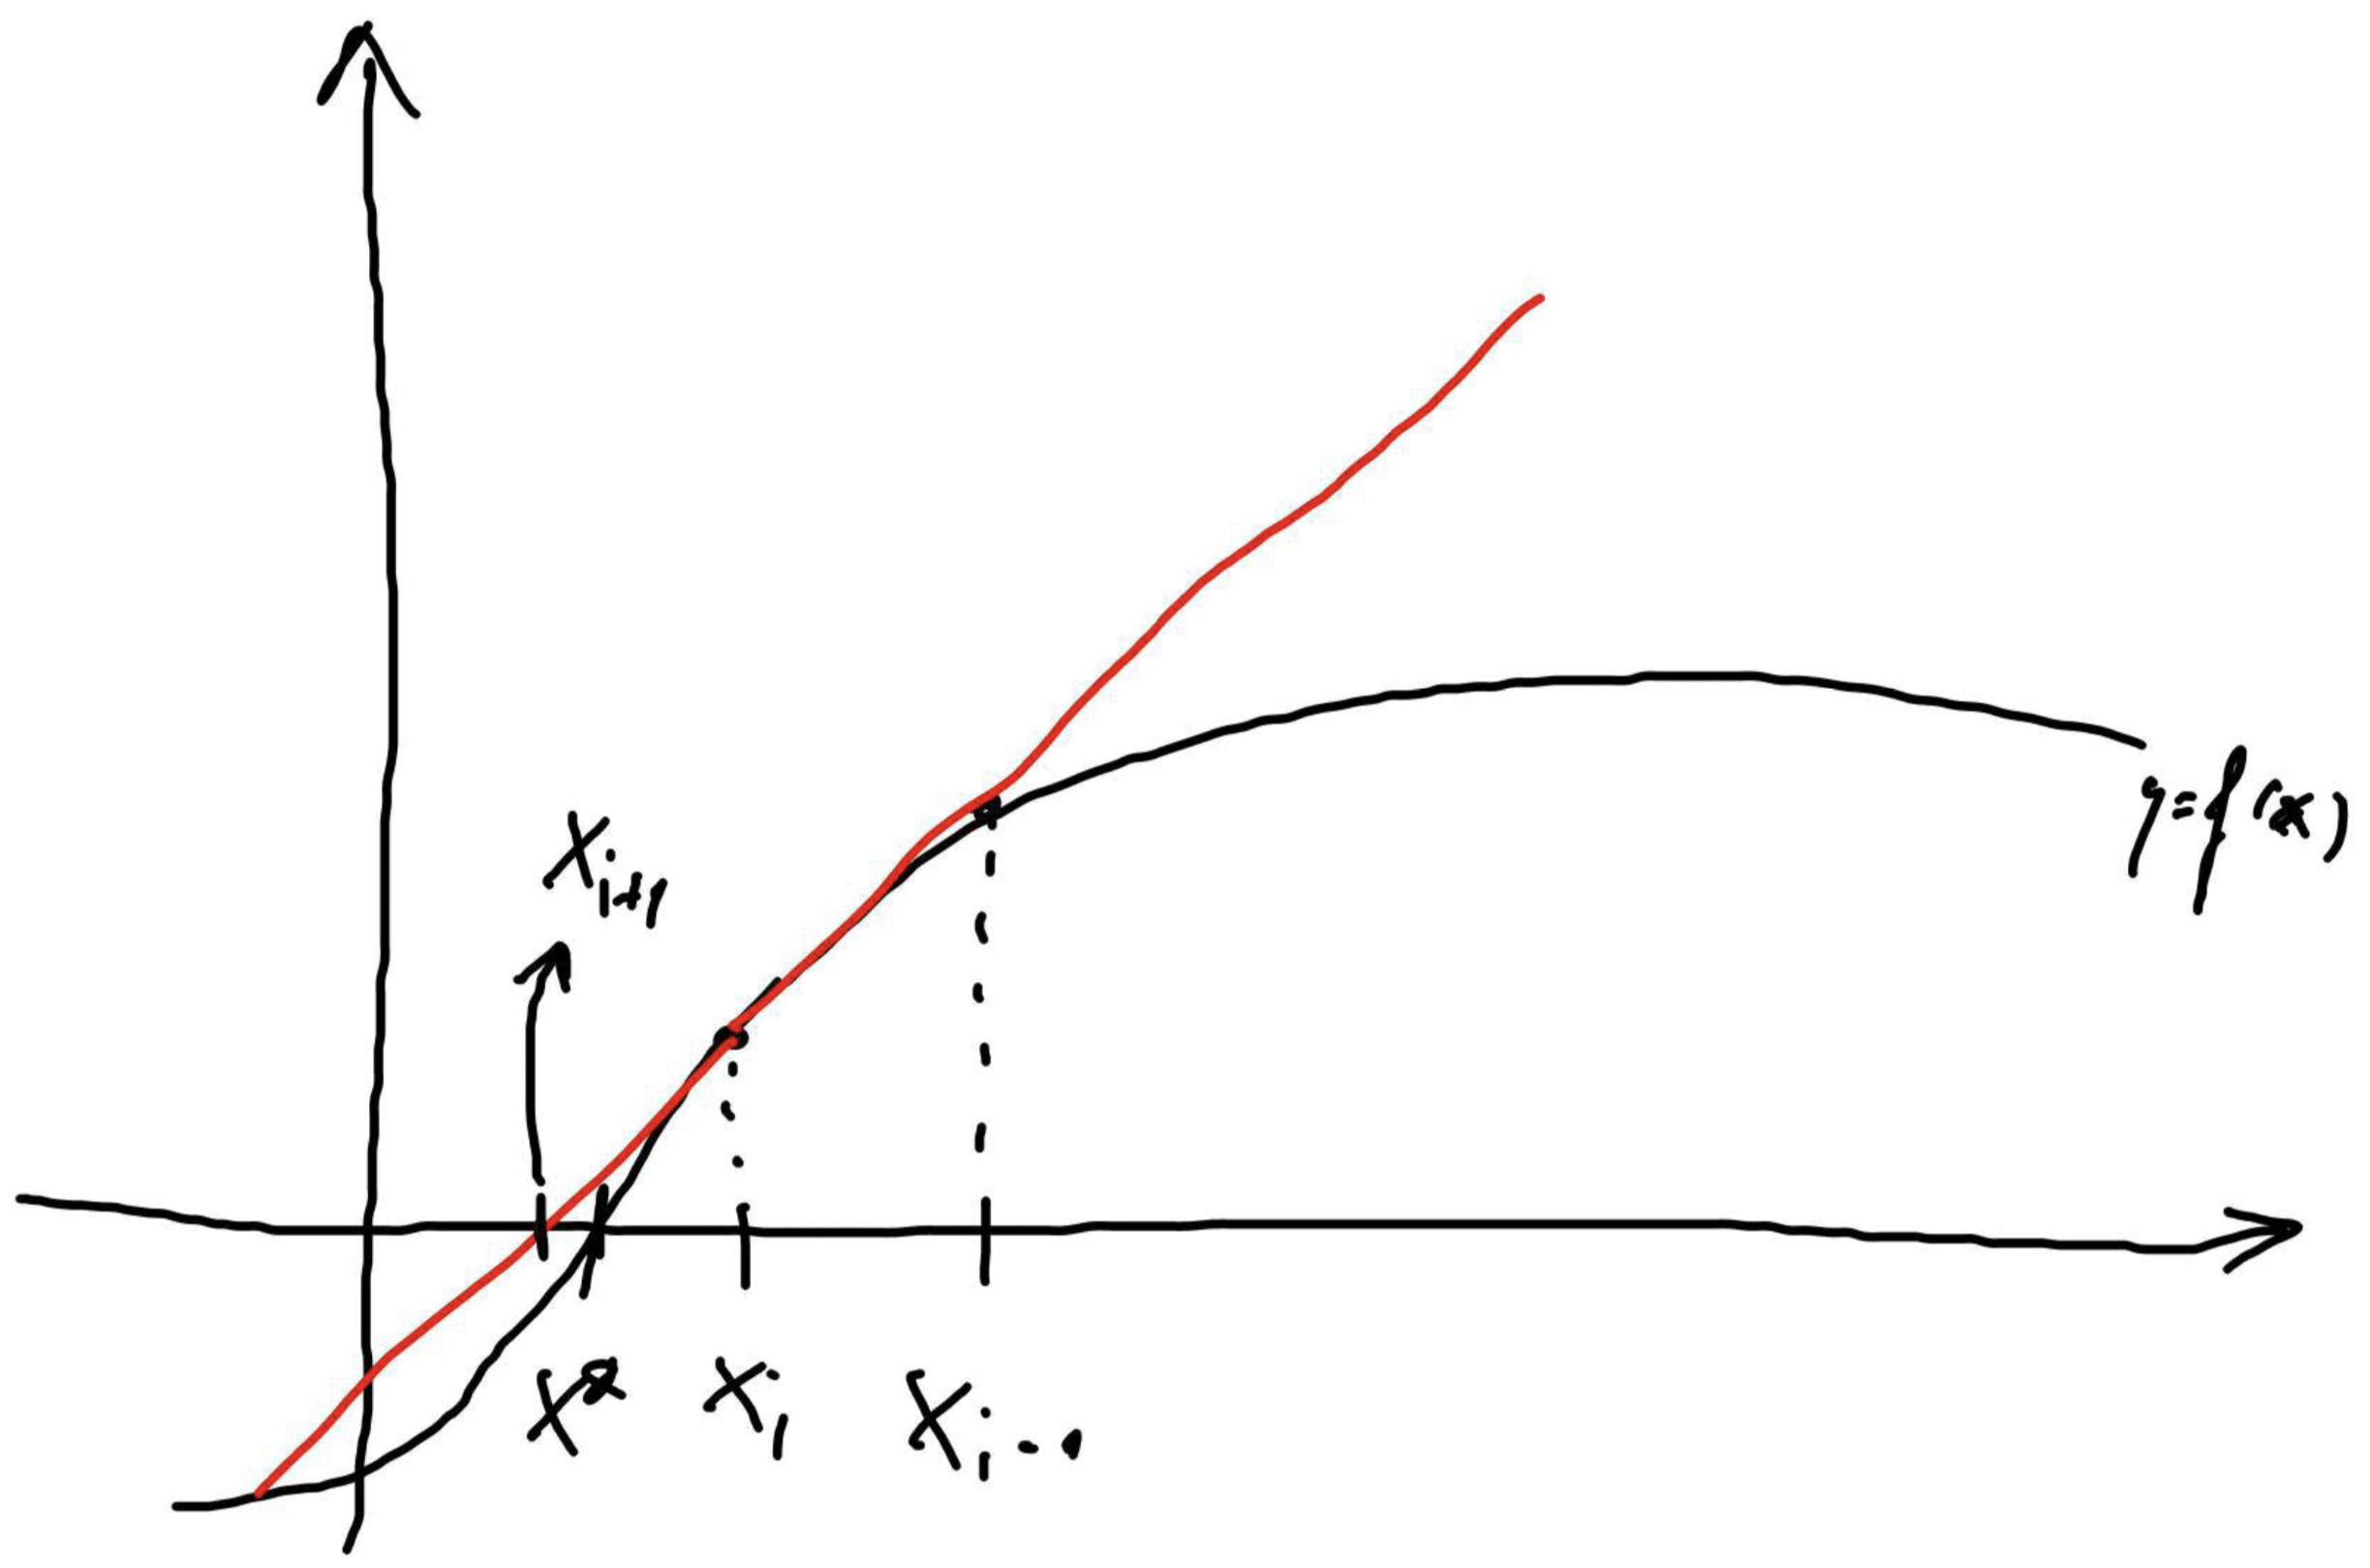
\includegraphics[width=0.5\textwidth]{immagini/GraficoSecanti.png}
	\caption{\label{fig:GraficoSecanti} Metodo delle secanti (\ref{eq:approxSecanti}). La linea rossa dovrebbe passare per $x_{i+1},\; x_i\; e\; x_{i-1}$.}
\end{figure}

\paragraph{Costo computazionale:}\footnote{Slide 9 PDF lez11.}
L'approssimazione (\ref{eq:approxSecanti}) richiede una valutazione funzionale per iterazione, in quanto $f(x_{i-1})$ è calcolato al passo $i-1$. La prima iterazione ne richiede due, ma sono trascurabili.

\paragraph{Convergenza:}\footnote{Slide 10 PDF lez11.} locale. Inoltre, il metodo delle secanti è superlineare, ovvero: la successione delle approssimazioni converge alla radice della funzione con un tasso di convergenza maggiore rispetto al metodo delle tangenti e al metodo della bisezione, ma minore rispetto al metodo di Newton.

\paragraph{Ordine di convergenza:} $p = \frac{\sqrt{5}+1}{2}\approx 1.618$ per radici semplici. Anche se l'ordine di convergenza è minore rispetto a quello del metodo di Newton è preferibile a quest'ultimo, in quanto non viene effettuata una valutazione della derivata ad ogni iterazione.

\begin{remark}
	Nella conversione dei precenti metodi in algoritmi è buona norma eseguire controlli sul demominatore, affinchè non siano svolte divisioni per 0. Nel caso dell'approssimazione di radici multiple, mediante il metodo di Newton modificato o il metodo di accelerazione Aitken, quando la derivata si annulla ed il valore della funzione è molto piccolo, significa che è stata raggiunta la migliore approssimazione possibile della soluzione.
\end{remark}

\begin{algorithm}
	\caption{Implementazione del metodo delle secanti.}\label{alg:metodo_secanti}
	\begin{lstlisting}[style=Matlab-editor]
		function xstar = secanti(fun, x0, x1, tol, itmax)
		% 
		% xstar = secanti(f, x0, x1, tol, itmax)
		% 
		% Calcola una approssimazione della radice di f(x) con tolleranza tol.
		% 
		% Input:
		%     f - identidicatore della function che implementa f(x);
		%     x0, x1 - punti iniziali;
		%     tol - accuratezza richiesta (default tol = 10^(-6));
		%     itmax - numero massimo di iterazioni (default itmax = 1000).
		% 
		% Output:
		%     xstar - approssimazione della soluzione.
		if nargin < 3
			error('numero di argomenti in ingresso errato')
		elseif nargin == 3
			tol =1e-6; itmax = 1000;
		elseif nargin == 4
			itmax = 1000;
		end
		
		if tol <= 0, error('tolleranza errata'); end
		if itmax <= 0, error('itmax errato'); end
		
		f0 = feval(fun, x0);
		f1 = feval(fun, x1);
		
		for i = 1:itmax
			if f0 == f1 && f1 ~= 0
				error('il metodo non converge');
			end
			
			xstar = (x0*f1 - x1*f0)/(f1 - f0);
			delta = abs(xstar - x1);
			
			if delta <= tol * (1 + abs(xstar))
				break
			elseif i < itmax
				x0 = x1; xstar = x1;
				f0 = f1; f1 = feval(fun,x1);
			end
		end
		
		if delta > tol * (1+abs(xstar))
			warning('accuratezza richiesta non raggiunta');
		end
		return
	\end{lstlisting}
\end{algorithm}

\section{Sistemi Lineari e Nonlineari}
Il problema di questa sezione è risolvere sistemi di \gls{equazioni lineari} (detti \gls{sistemi lineari}) e di \gls{equazioni nonlineari}. Tali sistemi sono della forma 
\begin{equation}\label{eq:sistema_equazioni_lineari}
    A\uline{x}=\uline b,
\end{equation}
dove $A=(a_{ij})\in{\mathbb R^{m\times n}}$ è la matrice dei coefficienti, $\uline x=(x_i)\in\mathbb R^n$ il vettore delle incognite (da determinare) e $\uline b\in\mathbb R^m$ il vettore dei termini noti. $A$ e $\uline b$ sono noti. Sarà assunto che $\boldsymbol{m\geq n}$ e che il rango di A sia massimo, ovvero $\boldsymbol{\rank(A)=n}$.

Nel caso in cui $\boldsymbol{m>n}$ allora sono presenti più equazioni che incognite ed in questo caso il sistema è detto \textbf{sistema sovradimensionato}. Questo caso sarà trattato nella Sezione \ref{ssec:sistemi_lineari_sovradimensionati} e nella \ref{ssec:risoluzione_sistemi_nonlineari}. Inizialmente, fino alla Sezione \ref{ssec:sistemi_lineari_sovradimensionati}, sarà considerato il caso in cui la matrice dei coefficienti è definita come $A\in\mathbb R^{n\times n}$ matrice quadrata, ovvero $m=n$.

\begin{definition}[Matrice nonsingolare]\label{def:matrice_nonsingolare}
    La matrice $A\in\mathbb R^{n\times n}$, quadrata, è \gls{nonsingolare} se \gls{rank(A)}$=n$ (\textbf{quindi} $\boldsymbol{\det(A)\neq 0}$) ed il sistema (\ref{eq:sistema_equazioni_lineari}) ha soluzione unica del tipo
    \begin{equation}\label{eq:solSistQuad}
        \uline x = A^{-1} \uline b.
    \end{equation}
\end{definition}
La soluzione (\ref{eq:solSistQuad}) è una risoluzione del problema che non definisce, in genere, un algoritmo efficiente di risoluzione dal punto di vista computazionale.

\begin{definition}[Matrice singolare]\label{def:matrice_singolare}
	La matrice $A\in\mathbb R^{n\times n}$, quadrata, è \gls{singolare} se $\rank(A)\neq n$ (\textbf{quindi} $\boldsymbol{\det(A) = 0}$).
\end{definition}

\begin{remark}
    Con "costo computazionale" è da intendersi il costo in termini di occupazione di memoria e numero di operazioni floating-point richieste.
\end{remark}

\subsection{Sistemi lineari: casi semplici}\footnote{Slide 5 PDF 1, PG 41.}
La risoluzione del sistema lineare (\ref{eq:sistema_equazioni_lineari}) risulta agevole nel caso in cui $A$ abbia proprietà strutturali particolari, ovvero quando $A$ è:
\begin{itemize}
    \item diagonale,
    \item triangolare,
    \item ortogonale.
\end{itemize}
Queste caratteristiche saranno utilizzate per definire opportuni metodi di fattorizzazione che consentiranno di risolvere il problema generale.

\subsubsection{Caso \texorpdfstring{$\boldsymbol A$}{A} diagonale}\footnote{Slide 6 PDF 1, PG 42.}
In questo caso gli elementi non appartenenti alla diagonale di $A$ sono nulli, ovvero $A$ è della forma
\begin{equation*}
    \begin{pmatrix}
        a_{11}&&\\
        &\ddots&\\
        &&a_{nn}
    \end{pmatrix},
\end{equation*}
dove, per ogni $i,j=1,\hdots, n$, gli elementi $ a_{ij}=0$ se $j\neq i$ mentre $a_{ii}\neq 0,$ sono gli elementi della diagonale principale di $A$. La matrice dei coefficienti del sistema lineare \ref{eq:sistema_equazioni_lineari}) si fatta può esssere memorizzata come un singolo vettore.

\begin{remark}
    Per matrici grandi e con molti elementi nulli può essere utile l'Osservazione \ref{rem:diagonali}.
\end{remark}

Il determinante di $A$, se diagonale, è dato da $\det(A)=\prod_{i=1}^n a_{ii}.$ Pertanto, assunto $\det(A)\neq 0$, segue che $\boldsymbol{a_{ii}\neq 0,\, \forall i=1,\hdots,n}.$ Inoltre, dato che $A$ è diagonale, la \gls{forma component-wise} del sistema lineare (\ref{eq:sistema_equazioni_lineari}) è del tipo
\begin{equation*}
    \begin{matrix}
        a_{11} x_1 &=& b_1\\
        a_{22} x_2 &=& b_2\\
        &\vdots&\\
        a_{nn}x_n &=& b_n
    \end{matrix}
\end{equation*}
e quindi le componenti della soluzione possono essere calcolate come
\begin{equation}\label{eq:soluzione_matrice_diagonale}
    \boldsymbol{x_i=\frac{b_i}{a_{ii}},\; i=1,\hdots, n.}
\end{equation}

Questo algoritmo è ben definito, in quanto $a_{ii}\neq 0,\, \forall i=1,\hdots,n$ per ipotesi. 

\paragraph{Costo computazionale dell'algoritmo (\ref{eq:soluzione_matrice_diagonale}):} La complessità dell'algoritmo (\ref{eq:sistema_equazioni_lineari}) è $n$ flops e $O(n)$ memoria (si dice lineare perché richiede la memorizzazione di un vettore di lunghezza $n$).

\paragraph{Implementazione dell'algoritmo (\ref{eq:soluzione_matrice_diagonale}):} Un'implementazione naive di questo algoritmo è l'Algoritmo \ref{alg:implementazione_diagonale}.

\begin{algorithm}\caption{Risoluzione sistema lineare bidiagonale.}\label{alg:implementazione_diagonale}
    \begin{lstlisting}[style=Matlab-editor]
    function x = diago(a, b)
    	x = b./a;
    return
    end
    \end{lstlisting}
\end{algorithm} 

\subsubsection{Caso \texorpdfstring{$\boldsymbol A$}{A} triangolare}
Questo caso è a sua volta diviso in due, in quanto è necessario specificare dove si trovano gli elementi significativi della matrice, ovvero:
\begin{itemize}
    \item $A$ è \textbf{triangolare inferiore} $\iff a_{ij}=0,\, i<j$, ovvero la matrice è della forma 
        \begin{equation*}
            A=
            \begin{pmatrix}
                a_{11} & & \\
                \vdots & \ddots & \\
                a_{n1} & \hdots & a_{nn}
            \end{pmatrix};
    \end{equation*}
    \item $A$ è \textbf{triangolare superiore} $\iff a_{ij}=0,\, i>j$, ovvero la matrice è della forma
    \begin{equation*}
        A=
        \begin{pmatrix}
            a_{11} & \hdots & a_{1n}\\
                &\ddots & \vdots\\
             & & a_{nn}
        \end{pmatrix}.
    \end{equation*}
\end{itemize}

\noindent Per una generica matrice $A\in\mathbb R^{n\times n}$ triangolare (inferiore o inferiore), è noto che $\det(A)=\prod_{i=1}^n a_{ii}.$

\begin{remark}\footnote{Slide 9 PDF 1.}
    Se $A$ è contemporanemente triangolare inferiore e superiore, allora è diagonale.
\end{remark}

\subsubsubsection{Caso triangolare inferiore}
Nel caso in cui $A$ è triangolare inferiore, il sistema lineare (\ref{eq:sistema_equazioni_lineari}) è della forma
\begin{equation}\label{eq:sistema_lineare_triangolare_inferiore}
    \begin{matrix}
        a_{11} x_1 && && && &=& b_1\\
        a_{21} x_1 &+& a_{22} x_2 && && &=& b_2\\
        a_{31} x_1  &+& a_{32} x_2 &+& a_{33} x_3 && &=& b_3\\
        \vdots && && &\ddots& &\vdots &\vdots\\
        a_{n1} x_1 &+& a_{n1} x_2 &+& \hdots &+& a_{nn} x_n &=& b_n
    \end{matrix}
\end{equation}
e gli elementi della soluzione possono essere ottenuti mediante sostituzioni in avanti:
\begin{equation}\label{eq:soluzione_sistema_triangolare_inferiore}
    x_i=\frac{b_i-\overbrace{\sum_{j=1}^{i-1}a_{ij}x_j}^{\text{0 se $i=1$}}}{a_{ii}},\quad i=1,\hdots,n.
\end{equation}

L'algoritmo (\ref{eq:soluzione_sistema_triangolare_inferiore}) è ben definito sotto l'ipotesi $\det(A)\neq 0\; (\iff a_{ii}\neq 0,\; i=1,\hdots, n)$.

\paragraph{Costo computazionale dell'algoritmo (\ref{eq:soluzione_sistema_triangolare_inferiore}):} Per calcolare il numeratore sono necessarie $i-1$ moltiplicazioni, $i-1$ somme ed $1$ divisione finale (per calcolare $x_i$) per un totale di $2i-1$ \textit{flops}, quindi il costo totale è dato da
\begin{equation}\label{eq:flops_soluzione_sistema_triangolare_superiore}
    \sum_{i=1}^n(2i-1)=2\sum_{i=1}^n (i)-n= \cancel{2}\cdot\frac{n(n+1)}{\cancel{2}}-n=\boldsymbol{n^2\; flops}.
\end{equation}

L'occupazione di memoria è dovuta alla porzione triangolare della matrice e dai due vettori ($\uline x$ e $\uline b$), quindi:
\begin{equation*}
    \sum_{i=1}^n i = \frac{n(n+1)}{2}+ \overset{\text{vettori}}{2n}\approx \boldsymbol{\frac{n^2}{2}}\text{ \textbf{locazioni di memoria}.}
\end{equation*}

\paragraph{Implementazione risolutore sistema lineare con A triangolare inferiore:} È possibile codificare la soluzione al sistema triangolare inferiore (\ref{eq:soluzione_sistema_triangolare_inferiore}) con l'Algoritmo \ref{alg:calcSistTriangInf}. Per accedere alla matrice per colonne è sufficiente scambiare i cicli (vedere Algoritmo \ref{alg:calcSistTriangInf1}). Un'implementazione efficiente della soluzione di un sistema triangolare inferiore (\ref{eq:soluzione_sistema_triangolare_inferiore}) è l'Algoritmo \ref{alg:trilow}, il quale risolve il problema in modo vettoriale per colonne.

Il ciclo interno dell'Algoritmo \ref{alg:calcSistTriangInf} è un prodotto scalare (\textit{scal}). Il ciclo interno dell'Algoritmo \ref{alg:calcSistTriangInf1} è una \textit{axpy} (ovvero un'operazione del tipo vettore = scalare $\times$ vettore + vettore). Pertanto, è necessario osservare che il risultato di \textit{scal} e \textit{axpy} è simile ma non uguale, le operazioni sono diverse ed in arimetica finita l'errore si propaga.

\begin{algorithm}\caption{Sistema triangolare inferiore.}
\label{alg:calcSistTriangInf}
    \begin{lstlisting}[style=Matlab-editor]
    % a <-  matrice dei coefficienti
    % b <-  vettore dei termini noti
    % x <-  vettore soluzione
    %
    % x <- b rappresenta b_i in x_i
    for i = 1 : n
        for j = 1 : i-1
            x(i) = x(i) - a(i,j) * x(j);
        end
        x(i) = x(i) / a(i,i);
    end
    \end{lstlisting}
\end{algorithm}

\begin{algorithm}\caption{Sistema triangolare inferiore per colonne.}
\label{alg:calcSistTriangInf1}
    \begin{lstlisting}[style=Matlab-editor]
    % x <- b
    for j = 1 : n
     x(j) = x(j) / a(j,j);
        for i = j+1 : n
            x(i) = x(i) - a(i,j) * x(j);
        end
    end
    \end{lstlisting}
\end{algorithm}

\subsubsubsection{Caso triangolare superiore}
Nel caso in cui $A$ sia triangolare superiore, ovvero
\begin{equation*}
    A= 
\begin{bmatrix}
   a_{11} & a_{12} & \hdots & \hdots & a_{1n}\\
          & a_{22} & \hdots & \hdots & a_{2n}\\
          && \ddots & &\vdots\\
          &&& a_{n-1,n-1} & a_{n-1,n}\\
          & & & & a_{nn}
\end{bmatrix},
\end{equation*}
con $\det(A)=\prod_{i=1}^n a_{ii}\neq 0\iff a_{ii}\neq 0,\, i = 1,\hdots, n$, il sistema di equazioni lineari (\ref{eq:sistema_equazioni_lineari}) è della forma
\begin{equation*}
    \begin{matrix}
        a_{11} x_1 &+& a_{12} x_2 &+& \cdots &+& a_{1n} x_n &=& b_1\\
        && a_{22}x_2 &+& \cdots &+& a_{2n}x_n &=& b_2\\
        && &\ddots& && \vdots &\vdots& \vdots\\
        && && && a_{nn}x_n &=& b_n
    \end{matrix}
\end{equation*}
e gli elementi della soluzione possono essere ottenuti mediante sostituzioni in avanti:
\begin{equation}\label{eq:solSistTriangSup}
    x_i=\frac{b_i-\overbrace{\sum_{j=i+1}^{i-1}a_{ij}x_j}^{\text{0 se $i=1$}}}{a_{ii}},\quad i=n, n-1, \hdots, 1.
\end{equation}

\paragraph{Implementazione della soluzione al sistema triangolare superiore:} La codifica di questo algoritmo (vedi Algoritmo  \ref{alg:soluzione_sistema_triangolare_superiore}) segue condiderazioni simili a quelle viste per il caso triangolare inferiore riguardo ai costi (vedere (\ref{eq:flops_soluzione_sistema_triangolare_superiore})). Un'implementazione efficiente che risove un sistema triangolare superiore, in modo vettoriale e per colonne, è dato dall'Algoritmo \ref{alg:triu}.

\begin{algorithm}\caption{Sistema triangolare superiore.}
\label{alg:soluzione_sistema_triangolare_superiore}
    \begin{lstlisting}[style=Matlab-editor]
    x = b
    for i = n : -1 : 1
        for j = i+1 : n
            x(i) = x(i) - a(i,j) * x(j); % scal (prodoto scalare)
        end
        x(i) = x(i) / a(i,i);
    end
    \end{lstlisting}
\end{algorithm}

\begin{algorithm}\caption{Sistema triangolare superiore con accesso per colonne.}
\label{alg:soluzione_sistema_triangolare_superiore_colonne}
    \begin{lstlisting}[style=Matlab-editor]
    x = b
    for j = n : -1 : 1
        x(j) = x(j) / a(j,j);
        for i = 1 : j-1
            x(i) = x(i) - a(i,j) * x(j);
        end
    end
    \end{lstlisting}
\end{algorithm}

\begin{algorithm}
	\caption{Implementazione efficiente (vettoriale per colonne) risolutore sistema triangolare superiore.}\label{alg:triu}
	\begin{lstlisting}[style=Matlab-editor]
		function y = triu(U, b)
		%   
		%   y = triu(U, b)
		%
		%   Risolve un sistema triangolare superiore
		%
		% Input:
		%   U   -  matrice dei coefficienti;
		%   b  -   termine noto;
		%   
		% Output:
		%   y   -   vettore soluzione.
		%
		% Le prossime tre righe sono controlli iniziali.
		[m,n] = size(U);
		if m ~= n, error('Matrice non quadrata'), end
		if n~= length(b), error('Termine noto non consistente'), end
		
		y=b(:); %trasformazione di b in vettore colonna
		
		for i = n : -1 : 1
		if U(i,i) == 0, error('Matrice singolare'), end
		y(i) = y(i)/U(i,i);
		y(1:i-1) = y(1:i-1) - L(1:i-1, i)*y(i):
		end
		return
	\end{lstlisting}
\end{algorithm}

\paragraph{Nota sul ciclo interno dell'Algoritmo \ref{alg:soluzione_sistema_triangolare_superiore}:} \footnote{Slide 3 PDF 2.}
Data (\ref{eq:solSistTriangSup}), invece di calcolare prima la sommatoria in un ciclo, sottrarla a $b_i$ e dividerla per $a_{ii},\, b_i-\sum_{j=i+1}^{i-1}a_{ij}x_j$ è calcolata nel seguente modo: $x(i)$ è aggiornato con il valore precedente sotratto allo scalare $a(i,j)*x(j)$, dove, per $i=n$, inizialmente $x(i)$ contiene $b(i)(=b(n))$ con $j$ che varia ed $i$ che rimane fisso. Inoltre è un prodotto scalare.

Il relativo costo in termini di spazio e numero di operazioni è \textbf{identico} all'algoritmo del caso triangolare inferiore, ovvero rispettivamente $\frac{n^2}{2}$ e $n^2$. 

L'Algoritmo \ref{alg:soluzione_sistema_triangolare_superiore} accede agli elementi della matrice $A$ \textbf{per righe}. È possibile ottenere la corrispendente versione che accede ad a \textbf{per colonne} scambiando l'ordine dei due cicli for (vedere Algoritmo \ref{alg:soluzione_sistema_triangolare_superiore_colonne}).

Il ciclo interno dell'Algoritmo \ref{alg:soluzione_sistema_triangolare_superiore_colonne} è una \textit{axpy}.

\begin{remark}\footnote{Slide 4 PDF 2.}
    Una \textit{axpy} con vettori di lunghezza $n$ ha lo stesso costo di una \textit{scal} con vettori della stessa dimensione: $\boldsymbol{2n\, flops}$, dove 2 sono il numero di operazioni per ogni ciclo ed $n$ è il numero di cicli.
\end{remark}

Pertanto, sono enunciate alcune importante proprietà (enunciati$\backslash$lemmi) delle matrici triangolari, le quali saranno utilizzate (quindi è necessario conoscerle): \footnote{Slide 4 PDF 2}
\begin{enumerate}
    \item \footnote{Lemma 3.1 PG 45.} La somma di matrici triangolari inferiori ($\backslash$superiori) è una matrice triangolare inferiore ($\backslash$superiore);
    \item Il prodotto di due matrici triangolari inferiori ($\backslash$superiori) è una matrice triangolare inferiore ($\backslash$superiore). Gli elementi diagonali del prodotto sono dati dal prodotto degli elementi diagonali omologhi dei due fattori;
    \item \footnote{Proprietà derivata dalla 2. Lemma 3.3 PG 45.} La matrice inversa di una matrice triangolare inferiore ($\backslash$superiore) \gls{nonsingolare} è triangolare inferiore ($\backslash$superiore). I suoi elementi diagonali sono dati dai reciproci degli elementi diagonali omologhi;
    \item  \footnote{Lemma 3.2 PG 45.} Il prodotto di due matrici triangolari inferiori ($\backslash$superiori) a diagonali unitaria (ovvero con elementi diagonali tutti uguali ad $1$) è una matrice triangolare inferiore ($\backslash$superiore) a diagonale unitaria; \footnote{Il motivo è dovuto al fatto che la diagonale sia 1 e che gli elementi della diagonale siano calcolati dal prodotto degli elementi omonimi delle diagonali delle matrici (i quali sono tutti 1).}
    \item La matrice inversa di una matrice triangolare inferiore ($\backslash$superiore) \textbf{a diagonale unitaria} è una matrice triangolare inferiore ($\backslash$superiore) a diagonale unitaria;
\end{enumerate}

\begin{proof}[Dimostrazione della proprietà 2]
    \footnote{Slide 5 PDF 2.}
    Sarà esaminato il caso triangolare inferiore, il caso triangolare superiore è anologo. Siano $A=(a_{ij}),\, B=(b_{ij})\in\mathbb R^{n\times n},$ con $a_{ij}=0=b_{ij},\, j>i$ (ovvero $A$ e $B$ sono triangolari inferiori) e sia $C=(c_{ij})=A\cdot B.$ È necessario dimostrare che, $\forall i=1,\hdots, n$:
    \begin{itemize}
        \item[1)] $c_{ij}=0,\quad j>i;$
        \item[2)] $c_{ii}=a_{ii}\cdot b_{ii},\quad i=j$.
    \end{itemize}
    Dalla 1) è ottenuto
    \begin{equation*}
        c_{ij}\overset{\footnotemark}{=}\uline e_i^T\,C\,\uline e_j=\underbrace{(\uline e_i^T\, \overbrace{A)\cdot(B}^{C}\,\uline e_j)}_{\footnotemark}=(\overbrace{a_{i1}\cdots a_{ii}}^{i}\, \overbrace{0\cdots 0}^{n-i})(\overbrace{0\cdots 0}^{j-1}\overbrace{b_{jj}\cdots b_{nj}}^{n-j+1})^T\underset{\footnotemark}{\overset{\boldsymbol{j>i}}{=}}0.
    \end{equation*}
    
    \addtocounter{footnote}{-2}
    \footnotetext{Tramite il prodotto $e_i^T\,C$ è ottenuta l'$i$-esima riga di $C$. Tramite il prodotto $C\cdot e_j$ è ottenuta l'$j$-esima riga di $C$.}
    
    \stepcounter{footnote}
    \footnotetext{Prodotto scalare tra riga $i$-esima di $A$ e la riga $j$-esima di $B$.}
    
    \stepcounter{footnote}
    \footnotetext{Oppure $j-1\geq i$.}
    
    \noindent Dalla 2), ovvero il caso $i=j$, con argomenti analoghi è ottenuto
    \begin{equation*}
        c_{ii}=(\overbrace{a_{i1}\cdots a_{ii}}^{i}\,\overbrace{0\cdots 0}^{n-i})(\overbrace{0\cdots 0}^{i-1}\,\overbrace{b_{ii}\cdots b_{ni}}^{n-i+1})^T=\underbrace{a_{ii}\cdot b_{ii}}_{\footnotemark}.
    \end{equation*}
    \footnotetext{$ii$ perché le moltiplicazioni sono svolte tra $a$ con indici precedenti ad $ii$ sono per 0 (ovvero gli $(i-1)\cdot 0$), così anche per le $b$ con indici maggiori di $ii$.}
\end{proof}

\begin{algorithm}
	\caption{Implementazione efficiente risolutore sistema triangolare inferiore.}\label{alg:trilow}
	\begin{lstlisting}[style=Matlab-editor]
		function y = trilow(L, b)
		%   
		%   y = trilow(L, b)
		%
		%   Risolve un sistema triangolare inferiore
		%
		% Input:
		%   L   -  matrice dei coefficienti;
		%   b  -   termine noto;
		%   
		% Output:
		%   y   -   vettore soluzione.
		%
		% Le prossime tre righe sono controlli iniziali.
		[m,n] = size(L);
		if m ~= n, error('Matrice non quadrata'), end
		if n~= length(b), error('Termine noto non consistente'), end
		
		y=b(:); %trasformazione di b in vettore colonna
		
		for i = 1 : n
		if L(i,i) == 0, error('Matrice singolare'), end
		 y(i) = y(i)/L(i,i);
		 y(i+1:n) = y(i+1:n) - L(i+1:n, i)*y(i):
		end
		return
	\end{lstlisting}
\end{algorithm}

\subsubsection{Caso \texorpdfstring{$\boldsymbol A$}{A} ortogonale}
\begin{definition}[Matrice Ortogonale]
    \footnote{Slide 6 PDF 2, PG 45.} $\boldsymbol A$ \textbf{è ortogonale se} $\boldsymbol{A^TA=AA^T=I.}$
\end{definition}
Pertanto, se $A$ è ortogonale, allora $A^{-1}=A^T.$ In questo caso, la soluzione a (\ref{eq:sistema_equazioni_lineari}) è data da $\uline x = A^T\uline b.$ Quindi il problema è risolto mediante un \textbf{prodotto matrice-vettore (\textit{matvec})}.

%\vspace{5px}
%\hrule
%\vspace{-7px}
\paragraph{Divagazione sul costo ed accesso ai dati per l'esecuzione di una \textit{matvec}.} Supponendo di voler calcolare $\uline y= A \uline x,$ dove $A\in\mathbb R^{m\times n},\,\uline x\in\mathbb R^n,\, \uline y\in\mathbb R^m$ \footnote{Il caso in cui $m=n$ e un caso particolare di $\mathbb R^{m\times n}$.} è possibile distinguere il caso in cui $A$ è rappresentato per righe e per colonne.

\begin{itemize}
    \item $A$ per righe è della forma $(a_{ij})=A=
    \begin{bmatrix}
        \boldsymbol{\uline r_1^T}\\
        \boldsymbol{\uline r_2^T}\\
        \vdots\\
        \boldsymbol{\uline r_m^T}\\
    \end{bmatrix},$ con $\boldsymbol{\uline r_i^T=(a_{i1}, \hdots, a_{in})}$ la $i$-esima riga di $A,\, i=1,\hdots, m$;
    \item $A$ per colonne è della forma $A=[\boldsymbol{\uline c_1\, \uline c_2\, \cdots\, \uline c_n}],$ con $\boldsymbol{\uline c_j}=
    \begin{bmatrix}
        \boldsymbol{a_{1j}}\\
        \boldsymbol{a_{2j}}\\
        \vdots\\
        \boldsymbol{a_{mj}}
    \end{bmatrix}$ la $j$-esima colonna di $A$, $j=1,\hdots, n.$
    \end{itemize}

\noindent Siano $y_{i\in\{1,\hdots, m\}}$ la $i$-esima componente di $\uline y$ e con $x_{j\in\{1,\hdots, n\}}$ la $j$-esima componente di $\uline x,\;\uline y$ può essere calcolata come $y_i=\boldsymbol{\uline r_i^T \uline x},\, i=1,\cdots, m$. L'implementazione del calcolo di $y_i$ è l'Algoritmo \ref{alg:matvecRiga} (il quale ha un costo di $\boldsymbol{2mn\, flops}$).

\begin{algorithm}
    \caption{$y_i= r_i^T \uline x$ in pseudo-codice.}
    \label{alg:matvecRiga}
    \begin{algorithmic}
        \State $y\gets 0$
        \For{i = 1 : m}
            \For{j = 1 : n}
               \State $y(i)=y(i)+\underset{\footnotemark}{\boldsymbol{\uline{a(i,j)}}}*x(j)\quad |$ scal
            \EndFor
        \EndFor
    \end{algorithmic}
\end{algorithm}
\footnotetext{Accesso per riga.}

È possibile ottenere una corrispondente implementazione con accesso per colonna scambiando i cicli for e, quindi, svolgendo una \textit{axpy}, osservando che: $\uline y= \uline c_1 x_1+ \hdots +\uline c_n x_n=\sum_{j=1}^n\uline c_j x_j.$
%\vspace{5px}
\hrule
%\vspace{-7px}
\paragraph{Metodi di fattorizzazione}\footnote{Slide 9-11 PDF 2, PG 46.} Nel caso in cui $A$ sia una generica matrice \gls{nonsingolare} allora è utile che questa sia fattorizzata nel prodotto di un numero, $k$ (in genere $k=1,2$), di fattori $F_1,\, F_2,\,\hdots,\, F_k\in\mathbb R^{n\times n}$ semplici. Questo significa che:
\begin{enumerate}
    \item $A=F_1\cdots F_k;$
    \item $F_i\,\begin{cases}
        \text{diagonale}\\
        \text{triangolare}\\
        \text{ortogonale}
    \end{cases}$ con $i=1,\hdots, k.$
\end{enumerate}

Pertanto, è possibile risolvere $A\uline x=\uline b$  è possibile risolvere $F_1 \cdots F_k \, \uline x=\uline b.$ Questo equivale a risolvere, ponendo $\uline x_0=\uline b$, i $k$ sistemi lineari
\begin{equation*}
 F_i \uline x_i = \uline x_{i-1},\, i=1,\hdots, k,
\end{equation*}
quindi, $\underset{\footnotemark}{\uline x_k}\equiv \uline x.$ \footnotetext{Soluzione equivalente ad $x$.}

\begin{example}
    Con $k=2,\, F_1 F_2 \, \uline x\overset{\footnotemark}{=}\uline b\Rightarrow\underset{\footnotemark}{F_1\, \uline x_1} = \uline x_0,\, \underset{\footnotemark}{F_2\, \uline x} = \uline x_1$
\end{example}

\addtocounter{footnote}{-2}
\footnotetext{È necessario risolvere prima $F_1\, x_1=x_0$ e poi $F_2 \, \uline x = x_1$, altrimenti cambia il risultato.}

\stepcounter{footnote}
\footnotetext{Dal prodotto risulta un vettore con $m$ righe. $m$ è comune alla matrice $F_2$ ed al vettore $\uline x$, altrimenti non sarebbe possibile effettuare il prodotto.}

\stepcounter{footnote}
\footnotetext{$F_2 \, \uline x=\uline x_1$ e $b=\uline x_0$.}

I due sistemi lineari (in genere saranno $k$) sono di tipo semplice e quindi sono possono essere risolti agilmente.

I metodi che consistono nel determinare dei fattori che soddisfano i precedenti punti, 1. e 2., sono detti \textbf{metodi di fattorizzazione}.

Inoltre, è possibile osservare che non è necessario memorizzare tutte le soluzioni intermedie $x_1,\hdots, x_k\equiv x$. Una volta calcolata la soluzione intermedia $x_i$, le precedenti non saranno utilizzate. Pertanto, è possibile utilizzare un unico vettore che, inizialmente, contiene il vettore dei termini noti e viene sovrascritto con le soluzioni intermedie, fino ad ottenere la soluzione finale del sistema lineare (\ref{eq:sistema_equazioni_lineari}).

\subsection{Fattorizzazione \texorpdfstring{$\boldsymbol{LU}$}{LU} di una matrice}
\begin{definition}[Matrice fattorizzabile $LU$]\footnote{Slide 2 PDF 3, PG 47.}
    Data $A$, matrice dei coefficienti del sistema (\ref{eq:sistema_equazioni_lineari}), questa si dice \textbf{fattorizzabile} $\boldsymbol{LU}$ se rappresentabile nella forma
    \begin{equation}\label{eq:ALU}
        \boldsymbol{A=L\cdot U},
    \end{equation}
   con:
    \begin{itemize}
        \item $\boldsymbol L$ è una matrice \textbf{triangolare inferiore a \ul{diagonale unitaria}}, ovvero: 
        \begin{equation*}
            L=(l_{ij}),\, \boldsymbol{l_{ij}=0,\, j>i,\, \forall i,j=1,\hdots, n};
        \end{equation*}
        \item $\boldsymbol U$ è \textbf{triangolare superiore}, ovvero $U=(u_{ij}),\, \boldsymbol{u_{ij}=0,\, i>j,\, \forall i,j=1,\hdots, n}$ (condizione restritiva).
    \end{itemize}
\end{definition}

\begin{definition}[Matrice a diagonale unitaria]
	Si dice che $A\in\mathbb{R}^{n\times n}$ è a diagonale unitaria se $a_{ii}=1,\, \forall i=1,\hdots, n$.
\end{definition}

\begin{remark}\footnote{Slide 3 PDF 3.}
    Se $A$ è fattorizzabile $LU$ allora, risolvere il sistema lineare (\ref{eq:sistema_equazioni_lineari}), significa risolvere
    \begin{equation*}
        L\, \underbrace{\boldsymbol{U\uline x}}_{\boldsymbol y}= \uline b.
    \end{equation*}
    Il problema sarà risolto mediante la risoluzione, \textbf{nell'ordine}, dei seguenti sistemi lineari di tipo \textbf{semplice}:
    \begin{equation*}
        L\uline y =\uline b,\quad U\uline x= \uline y.
    \end{equation*}
\end{remark}

\begin{theorem}[Unicità della fattorizzazione $LU$]\footnote{Slide 3 PDF 3, Teorema 3.1 PG 47.}\label{th:unicita_fattorizzazione_LU}
    Se $A$ è fattorizzabile $LU$ ed $A$ è \gls{nonsingolare} allora la fattorizzazione è unica. 
\end{theorem}
\begin{proof}
    \footnote{Slide 4 PDF 3, PG 47. È importante per successive trattazioni.} Supposto
    \begin{equation}\label{eq:uguaglianza_dimostrazione_LU_unica}
    	A=L\cdot U = L_1\cdot U_1,
    \end{equation}
     con:
    \begin{itemize}
        \item $L, L_1$ triangolari inferiori a diagonale unitaria;
        \item $U, U_1$ triangolari superiori.
    \end{itemize}
    È necessario verificare che
    \begin{equation*}
        L=L_1,\quad U=U_1.
    \end{equation*}
    Poiché
    \begin{equation*}
        0\neq\det(A)=\det(L\cdot U)= \overbrace{\det(L)}^{1}\cdot \det(U)=\det(U),
    \end{equation*}
    è possibile affermare che $U$ è \gls{nonsingolare}. In modo analogo $U_1$ è \gls{nonsingolare}.

    \noindent Dall'uguaglianza (\ref{eq:uguaglianza_dimostrazione_LU_unica}) è ottenuto, moltiplicando a sinistra, membro a membro, per $L_1^{-1}$ è ottenuto
    \begin{equation*}
        L_1^{-1}L\cdot U= \underbrace{L_1^{-1}L_1}_{I}\cdot U_1 = U_1,
    \end{equation*}
    quindi
    \begin{equation*}
    	L_1^{-1}L\cdot U= U_1.
    \end{equation*}

    \noindent Moltiplicando a destra, membro a membro, per $U^{-1}$ è ottenuto
    \begin{equation*}
    	\boldsymbol{L_1^{-1}L\cdot \underbrace{U\cdot U^{-1}}_I}=L_1^{-1}L\boldsymbol{=U_1U^{-1}}.
    \end{equation*}
    
    \noindent In conclusione: \begin{equation*}
        \boldsymbol{L_1^{-1}L}=\boldsymbol{U_1U^{-1}}.
    \end{equation*}
    È possibile osservare che:
    \begin{itemize}
    	\item \textbf{a primo membro}, $L_1$ è triangolare inferiore a diagonale unitaria allora $L_1^{-1}$ è triangolare inferiore a diagonale unitaria; poiché anche $L$ è triangolare inferiore a diagonale unitaria $\boldsymbol{L_1^{-1}L}$ \textbf{è triangolare inferiore a diagonale unitaria}.
        \item \textbf{a secondo membro}, $U$ è triangolare superiore, allora $U^{-1}$ è triangolare superiore; poiché anche $U_1$ è triangolare superiore, è possibile concludere che $\boldsymbol{U_1U^{-1}}$ \textbf{è triangolare superiore};
    \end{itemize}
    Da questo è concluso che $L_1^{-1}L=I=U_1U^{-1},$ ovvero:
    \begin{itemize}
        \item $L_1^{-1}L=I\Rightarrow L=L_1$,
        \item $U_1U^{-1}=I\Rightarrow U_1=U.$
    \end{itemize}
    Quindi è provata l'unicità della fattorizzazione di una matrice \gls{nonsingolare}.
\end{proof}

Sono date le seguenti definizioni utili prima di stabilire quale sia la condizione di esistenza della fattorizzazione $LU$ (Teorema \ref{th:esistenza_fattorizzazione_LU}).

\begin{remark}
    Affinché $A$ sia definita la fattorizzazione $LU\Rightarrow\det(U)\neq 0$.
\end{remark}

\subsubsection{Algoritmo di fattorizzazione \texorpdfstring{$\boldsymbol{LU}$}{LU}}

Al fine di definire un algoritmo per ottenere la fattorizzazione $LU$ di $A$, è considerato il seguente problema: dato un vettore $\uline v\in\mathbb R^n$, è supposto di voler definire una matrice $\boldsymbol {L\in\mathbb R^{n\times n}}$ \textbf{triangolare inferiore a diagonale unitaria} tale che:
\begin{equation}\label{eq:Lv}
    L\uline v \equiv L\cdot \begin{bmatrix}
        v_1\\
        v_2\\
        \vdots\\
        v_n
    \end{bmatrix}=[\overbrace{\boldsymbol{v_1,\cdots, v_k}}^{k}\overbrace{\boldsymbol{0,\cdots, 0}}^{n-k}]^T,
\end{equation}
dove $v_i$ è la $i$-esima componente di $\uline v$ e $k$ è un indice fissato a priori. $L$ deve azzerare in modo selettivo le componenti di $\uline v$, a partire dalla $(k+1)$-esima in poi, lasciando inalterate le prime $k$ componenti del vettore.

Supponendo $\boldsymbol{v_k\neq 0}$, ovvero l'ultima componente di $\uline v$ che rimane inalterata, è definito il corrispondente \textbf{vettore elementare di Gauss:}
\begin{equation}\label{eq:vettElemGauss}
    \uline g_k=\frac{1}{\boldsymbol{v_k}}[\overbrace{0\cdots 0}^k \underbrace{v_{k+1}\cdots v_n}_{\underset{\footnotemark}{n-k}}]^T
\end{equation}
\footnotetext{Numero di componenti da azzerare.}
e la relativa \textbf{matrice elementare di Gauss},
\begin{equation}\label{eq:matrElemGauss}
    L=I\boldsymbol - \uline g_k \uline e_k^T,
\end{equation}
dove $\uline e_k$ è il $k$-esimo vettore della base canonica di $\mathbb R^n$ definito come $\uline e_k=[0\cdots 0\,\overset{\footnotemark}{1}\, 0 \cdots 0]^T.$ 
\footnotetext{$k$-esimo elemento del vettore.}

È necessario dimostrare che:
\begin{enumerate}
    \item $L$ è triangolare inferiore a diagonale unitaria;
    \item $L$ soddisfa (\ref{eq:Lv}).
\end{enumerate}

\begin{proof}[Dimostrazione di 1]\footnote{Slide 8 PDF 3, PG 48.}
    Da (\ref{eq:matrElemGauss}) è ottenuto
    \begin{equation*}
        L = \begin{bmatrix}
            1 \\
            & \ddots & \footnotemark \\
            & & 1\\
            & & -\frac{v_{k+1}}{v_k}&\ddots\\
            & & \vdots & &\ddots\\
            & & -\frac{v_n}{v_k} & & & 1\\
        \end{bmatrix},\quad L\uline v=\begin{bmatrix}
            v_1\\
            \vdots\\
            v_k\\
            0\\
            \vdots\\
            0
        \end{bmatrix}
    \end{equation*}
    che è triangolare inferiore con diagonale unitaria.
\end{proof}
\footnotetext{Sotto l'$1$ c'è il vettore $\uline g_k$.}

\begin{proof}[Dimostrazione della 2]\footnote{Slide 7 PDF 3, PG 48.}
    $L\uline v\overset{\footnotemark}{=}\left(I-\uline g_k \uline e_k^T\right)\uline v= \uline v-\uline g_k\underbrace{\left(\uline e_k^T\uline v\right)}_{v_k} \overset{\footnotemark}{=}\uline v - \underset{\footnotemark}{\uline{\uline g_k v_k}}=\begin{bmatrix}
        v_1\\
        \vdots\\
        v_n
    \end{bmatrix}-
    \begin{bmatrix}
        0\\
        \vdots\\
        0\\
        v_{k+1}\\
        \vdots\\
        v_n
    \end{bmatrix}\overset{\footnotemark}{=}\begin{bmatrix}
        v_1\\
        \vdots\\
        v_k\\
        0\\
        \vdots\\
        0
    \end{bmatrix}.$
\end{proof}

\addtocounter{footnote}{-3}
\footnotetext{Sostituzione di $L$ con $(I-\uline g_k \uline e_k^T)$.}

\stepcounter{footnote}
\footnotetext{Sostituzione di $\uline i_k^T\uline v$ con $v_k$.}

\stepcounter{footnote}
\footnotetext{È possibile la semplificazione di $\frac{1}{v_k}[0\cdots 0\, v_{k-1}\cdots v_n]^T$ con $v_k$.}

\stepcounter{footnote}
\footnotetext{Il vettore sottratto è $\uline g_k$.}

\begin{theorem}\footnote{Slide 8 PDF 3, PG 48.}
    Sia $L$ la matrice elementare di Gauss definita come (\ref{eq:matrElemGauss}), allora:
    \begin{equation}
        L^{-1}=I\underset{\footnotemark}{\boldsymbol +}\uline g_k\uline e_k^T.
    \end{equation}
\end{theorem}
\footnotetext{Impotante che sia $+$ per ottenere $L^{-1}$ invertendo solamente il segno della parte inferiore della $k$-esima colonna.}

È possibile ora definire l'algoritmo di fattorizzazione $LU$. Questo algoritmo è \textbf{semi-iterativo}, ovvero ottiene la fattorizzazione, se esiste, in $n-1$ passi. Sarà utilizzata la notazione $a_{ij}^{(k)}$ per denotare il passo più recente dell'algoritmo, il $k$-esimo, in cui l'elemento $(i,j)$ di $A$ è stato modificato.

Data la matrice di partenza
\begin{equation}\label{eq:A1}
    A=\begin{bmatrix}
        a_{11}^{(1)} & \cdots & a_{1n}^{(1)}\\
        \vdots & & \vdots\\
        a_{n1}^{(1)}&\cdots & a_{nn}^{(1)}
    \end{bmatrix}\equiv A^{(1)},
\end{equation}
al primo passo di fattorizzazione è necessario definire una matrice triangolare inferiore a diagonale unitaria, in modo tale che $L_1 A^{(1)}=A^{(2)}$ abbia la prima colonna strutturalmente simile a quella di una matrice triangolare superiore (ovvero è necessario azzerare gli elementi dal secondo in poi).

Se $\boldsymbol{a_{11}^{(1)}\neq 0}$ (condizione necessaria e sufficiente), è possibile definire il primo vettore di Gauss,\begin{equation}\label{eq:1oVettElemGauss}
    \uline g_1=\frac{1}{a_{11}^{(1)}}\left[0\; a_{21}^{(1)}\cdots a_{n1}^{(1)}\right]^T
\end{equation}
e la corrispondente prima matrice elementare di Gauss, 
\begin{equation}
    L_1=I-\uline g_1\uline e_1^T=\begin{bmatrix}
        1\\
        -\frac{a_{21}^{(1)}}{a_{11}} & 1\\
        \vdots & &\ddots\\
        -\frac{a_{n1}^{(1)}}{a_{11}} & & &1
    \end{bmatrix},
\end{equation}
tali che
\begin{equation*}
    L_1 A\overset{\footnotemark}{=}
    \begin{bmatrix}
        a_{11}^{\boldsymbol{(1)}} & a_{12}^{\boldsymbol{(1)}} & \hdots & a_{1n}^{\boldsymbol{(1)}}\\
        0 & \boldsymbol{a_{22}^{(2)}} & \boldsymbol\hdots & \boldsymbol{a_{2n}^{(2)}}\\
        \vdots & \boldsymbol\vdots & & \boldsymbol\vdots\\
        0 & \boldsymbol{a_{n2}^{(2)}} & \boldsymbol\hdots & \boldsymbol{a_{nn}^{(2)}}
    \end{bmatrix}\equiv A^{\boldsymbol{(2)}}.
\end{equation*}
\footnotetext{Gli elementi in grassetto sono modificati rispetto al passo precedente.}

Se $\boldsymbol{a_{22}^{(2)}\neq 0}$ è possibile definire il secondo vettore elementare di Gauss,
\begin{equation}\label{eq:2oVettElemGauss}
    \uline g_2 = \frac{1}{a_{22}^{(2)}}[\overbrace{0\, 0\,}^{2} a_{32}^{(2)}\hdots a_{n2}^{(2)}]^T,
\end{equation}
e la corrispondente seconda matrice elementare di Gauss,
\begin{equation*}
    L_2=I-\uline g_2\uline e_2^T=\begin{bmatrix}
        1 & & &\\
        & 1 & &\\
        & -\frac{a_{32}^{(2)}}{a_{22}} & \ddots &\\
        & \vdots &&\ddots\\
        & -\frac{a_{n2}^{(2)}}{a_{22}}  & & & 1
    \end{bmatrix},
\end{equation*}
tale che 
\begin{equation*}
    L_2\, L_1\, A = 
    \begin{pmatrix}
        a_{11}^{(1)} & a_{12}^{(1)} & a_{13}^{(1)} & \hdots & a_{1n}^{(1)}\\
        0 & a_{22}^{(2)} & a_{23}^{(2)} & \hdots & a_{2n}^{2}\\
        0 & 0 & \boldsymbol{a_{33}^{(3)}} & \boldsymbol\hdots & \boldsymbol{a_{3n}^{(3)}}\\
        \vdots & \vdots & \vdots & &\vdots\\
        0 & 0 & \boldsymbol{a_{n3}^{(3)}} & \boldsymbol\hdots & \boldsymbol{a_{nn}^{(3)}}
    \end{pmatrix}\equiv A^{\boldsymbol{(3)}}.
\end{equation*}

Procedendo in modo analogo, dopo un totale di $n-1$ passi,  sarà ottenuto
\begin{equation}\label{eq:fattLU}
    \boldsymbol{\underbrace{L_{n-1}\cdot L_{n-2}\cdot\hdots\cdot L_1}_{L^{-1}}\, A}=
    \begin{bmatrix}
        a_{11}^{(1)} &\hdots &\hdots &\hdots & a_{1n}^{(1)} \\
        & a_{22}^{(2)} &\hdots &\hdots & a_{2n}^{(2)}\\
        & & a_{33}^{(3)} &\hdots & a_{3n}^{(3)}\\
        & & &\ddots & \vdots \\
        & & & & a_{nn}^{\boldsymbol{(n)}}
    \end{bmatrix}\equiv A^{\boldsymbol{(n)}}\boldsymbol{\equiv U}.
\end{equation}

\paragraph{Condizioni per l'algoritmo di fattorizzazione:}
L'algoritmo è utilizzabile (vedere il Teorema \ref{th:condDefFattLU} definito in seguito) se, all'$i$-esimo passo,
\begin{equation}\label{eq:condDefElemGauss}
    \underset{\footnotemark}{\boldsymbol{a_{ii}^{(i)}}}\boldsymbol{\neq 0,\quad i = 1,\hdots, n-1},
\end{equation}
\footnotetext{Elementi diagonali di $U$.}
il che permetterà di costruire i corrispondenti vettori di Gauss,
\begin{equation}
    \uline g_i = \frac{1}{a_{ii}^{(i)}}\big[\overbrace{0\hdots 0}^{\boldsymbol i}\,a_{i+1,i}^{(i)}\hdots, a_{ni}^{(i)}\big]^T,
\end{equation}
e la $i$-esima matrice elementare di Gauss,
\begin{equation}\label{eq:iamatrElemGauss}
    L_i\overset{\footnotemark}{\equiv} I-\uline g_i \uline e_i^T = 
    \begin{bmatrix}
        1 & & &\\
        & \ddots & &\\
        & & 1 &\\
        & & -\frac{a_{i+1,i}^{(i)}}{a_{ii}^{(i)}}&\ddots&\\
        & & \vdots & &\ddots &\\
        & & -\frac{a_{ni}^{(i)}}{a_{ii}^{(i)}} & & & 1
    \end{bmatrix},
\end{equation}
\footnotetext{Azzera gli elementi di $A^{(i)}$, in colonna $i$-esima, al di sotto dell'elemento diagonale.}
tali che
\begin{equation}\label{eq:A^i}
    \underset{\footnotemark}{L_iA^{(i)}} = L_i\cdots L_1 A=
    \begin{bmatrix}
        a_{11}^{(1)} & \hdots & \hdots & \hdots & \hdots & a_{1n}^{(1)}\\
        0 & \ddots & & & & \vdots\\
        \vdots & \ddots & a_{ii}^{(i)} & \hdots & \hdots & a_{in}^{(i)}\\
        \vdots & & 0 & a_{i+1,i+1}^{(i+1)} & \hdots & a_{i+1, n}^{(i+1)}\\
        \vdots & & \vdots & \vdots & & \vdots\\
        0 & \hdots & 0 & a_{n,i+1}^{(i+1)} & \hdots & a_{nn}^{(i+1)}
    \end{bmatrix}\equiv A^{(i+1)},\quad i = 1, \hdots, n-1.
\end{equation}
\footnotetext{Questa moltiplicazione ha un costo di $2n^4$ flops perché entrambe le matrici hanno dimensione $n\times n$. La moltiplicazione $A\uline v$ ha un costo di $2n^2$ perché $\uline v$ è un vettore colonna.}

\begin{theorem}\label{th:condDefFattLU}
    La procedura (\ref{eq:fattLU}) è definita s.se $a_{ii}^{(i)}\neq 0,\, i=1,\hdots, n.$
\end{theorem}
\begin{proof}
    Se $A$ è \gls{nonsingolare}, $U$ deve essere \gls{nonsingolare} e, quindi, è necessario che $a_{nn}^{(n)}\neq 0$, oltre alle condizioni (\ref{eq:condDefElemGauss}).
\end{proof}

\begin{remark}
    Date le matrici elementari di Gauss $L_1, \hdots, L_{n-1}$ in (\ref{eq:fattLU}), è possibile osservare che:
\begin{enumerate}
    \item sono triangolari inferiori a diagonale unitaria;
    \item il loro prodotto è ancora una matrice triangolare inferiore a diagonale unitaria;
    \item la matrice inversa di questo prodotto è ancora una matrice triangolare inferiore a diagonale unitaria.
\end{enumerate}
Inoltre, è possibile $L^{-1}=L_{n-1}\cdot L_{n-2}\cdots L_2\cdot L_1$ da cui, in virtù della (\ref{eq:fattLU}), è ottenuta la fattorizzazione $A=LU$.
\end{remark}

È necessario trattare l'organizzazione dei dati della fattorizzazione $LU$: 
\begin{itemize}
    \item Il fattore $U$, nella sua porzione significativa, ovvero gli elementi della parte triangolare superiore, può essere memorizzato nella porzione triangolare superiore di $A$, come esposto in (\ref{eq:fattLU});
    \item Il fattore $L$ può essere rappresentato come $L=(L_{n-1}\cdots L_1)^{-1}=L_1^{-1}\cdots L_{n-1}^{-1}$.
    Inoltre, se
    \begin{equation*}
        L_i=I\boldsymbol - \uline g_i\uline e_i^T\Rightarrow L_i^{-1}=I\boldsymbol + \uline g_i\uline e_i^T,
    \end{equation*}
    è possibile concludere, per un generico $n$, che
    \begin{equation}\label{eq:L=I+g1e1T}
        \begin{matrix}
            \boldsymbol L &\overset{\footnotemark}{=}& (I+\uline g_1 \uline e_1^T)(I+\uline g_2 \uline e_2^T)\cdots(I+\uline g_{n-1} \uline e_{n-1}^T) &=& I + \uline g_1 \uline e_1^T +\hdots + \uline g_{n-1} \uline e_{n-1}^T \\
            &=& \begin{bmatrix}
            1 & & &\\
            g_{21} & 1 & & \\
            \vdots & \ddots & \ddots\\
            g_{n1} & \hdots & g_{n,n-1} & 1
        \end{bmatrix}&\boldsymbol =& \boldsymbol{I+\sum_{i=1}^{n-1}\uline g_i \uline e_i^T}.
        \end{matrix}
    \end{equation}
    \footnotetext{L'ordine di moltiplicazione è importante.}
\end{itemize}

\begin{example}\footnote{Slide 5 PDF 4.}
    Per comprendere (\ref{eq:L=I+g1e1T}) è valutato il caso più semplice, ovvero con $n=3$:
    \begin{equation*}
        L=\left(I+\uline g_1 \uline e_1^T\right)\left(I+\uline g_2\uline e_2^T\right) = \underbrace{I\cdot I}_{I}+\underbrace{I\cdot \uline g_1 \uline e_1^T}_{\uline g_1 \uline e_1^T}+ \uline g_2 \uline e_2^T + \uline g_1 \underbrace{\left(\uline e_1^T \uline g_2\right)}_{0} \uline e_2^T = I+\uline g_1\uline e_1^T + \uline g_2 \uline e_2^T = I + \sum_{i=2}^2\uline g_i \uline e_i^T.
    \end{equation*}
\end{example}

\paragraph{Pregi della fattorizzazione $LU$:} Poiché al passo $i$-esimo è necessario azzerare gli elementi $a_{i+1,i}^{(i)}, \hdots, a_{ni}^{(i)}$, ovvero la sezione triangolare inferiore in colonna $i$, allora è possibile sovrascriverli come $\frac{a_{i+1,i}^{(i)}}{a_{ii}^{(i)}}, \hdots,\frac{a_{ni}^{(i)}}{a_{ii}^{(i)}},$ i quali sono gli elementi significativi del vettore $\uline g_i.$ Questi ultimi costituiscono gli elementi significativi, in colonna $i$, del fattore $L$.
In conclusione, $A$ sarà riscritta con l'informazione relativa ai suoi fattori $L$ ed $U$ come:
\begin{equation*}
    \begin{bmatrix}
        a_{11}^{(1)} &\hdots &\hdots &\hdots & a_{1n}^{(1)} \\
        g_{21} & a_{22}^{(2)} &\hdots &\hdots & a_{2n}^{(2)}\\
        g_{31} & g_{32} & a_{33}^{(3)} &\hdots & a_{3n}^{(3)}\\
        \vdots & \vdots & \ddots &\ddots & \vdots \\
        g_{n1} & \hdots & \hdots & g_{n, n-2} & a_{nn}^{(n)}
    \end{bmatrix},
\end{equation*}
dove la diagonale principale di $L$ è "ignorata" perché nota.\qed

\subsubsubsection{Costo computazionale}
È esaminato il costo computazionale in termine di operazioni algebriche (\textit{flops}) e di occupazione di memoria del metodo i eliminazione di Gauss. Per questo (\ref{eq:A^i}) è ridefinito, esplicitando la struttura $L_i$, come:
\begin{equation}\label{eq:A^iRiscr}
	A^{(i+1)} = L_iA^{(i)} = \left(I-\uline g_i \uline e_i^T\right)A^{(i)} = A^{(i)} - \underset{\footnotemark}{\uline g_i} \underset{\footnotemark}{\left(\uline e_i^T A^{(i)}\right)}.
\end{equation}

\addtocounter{footnote}{-1}
\footnotetext{Vettore colonna.}

\stepcounter{footnote}
\footnotetext{Vettore riga $\left(i-\text{esima di }A^{(i)}\right)$.}

Tuttavia:
\begin{itemize}
	\item le prime $i$ componenti di $g_i$ sono nulle, quindi le prime $i$ righe nella somma in (\ref{eq:A^iRiscr}) non sono modificate;
	\item $\uline e_i^T A^{(i)}$ è l'$i$-esima riga di $A^{(i)}$, la quale ha le prime $i-1$ componenti nulle. Inoltre, in colonna $i$, dato che al passo successivo gli elementi sotto $a_{ij}^{(k)}$ sono 0, non è necessario svolgere operazioni perché è noto che queste avranno come risultato l'azzeramento degli elementi al di sotto di quello diagonale.
\end{itemize}

Pertanto, saranno processate solo le ultime $(n-i)$ righe e colonne di $A^{(i)}$, svolgendo 2 operazioni per componente, per un totale di $2(n-i)^2$ flops e, sommando gli $n-1$ passi, è ottenuto:
\begin{equation}\label{eq:costo_fattorizzazione_LU}
	2\sum_{i=1}^{n-1}(n-i)^2=2\sum_{i=1}^{n-1}i^2\overset{\footnotemark}{\approx}\boldsymbol{\frac{2}{3}n^3}\text{ \textbf{flops}.}
\end{equation}
\footnotetext{Utilizzando la somma notevole $\sum_{i=1}^ni^2=\frac{n(n+1)(2n+1)}{6}\Rightarrow\sum_{i=1}^{n-1}i^2=\frac{(n-1)(n-1+1)((2n-1)+1)}{6}=\frac{(n-1)n(2n-1)}{6}$}

In termini di locazioni di memoria occupata, il metodo di eliminazione di Gauss non richiede memoria addizionale, in quanto la matrice $A$ in ingresso sarà riscritta con le informazioni relative ai fattori $L$ ed $U$.

È possibile verificare quanto specificato per il costo computazionale esaminando lo pseudo-codice dell'Algoritmo \ref{alg:fattLU} (vedere l'Algoritmo \ref{alg:LUfatt} per controlli significativi).

La soluzione di un sistema lineare con $A=LU$ è implementata nell'Algoritmo \ref{alg:LUsolve}.
\begin{algorithm}
	\caption{Fattorizzazione $LU$ di una matrice.}
	\label{alg:fattLU}
	\begin{lstlisting}[style=Matlab-editor]
		for i = 1 : n - 1 %passi della fattorizzazione
		if A(i,i) == 0, error('Matrice non fattorizzabile LU'); end
		A(i+1:n,i) = A(i+1:n, i)/A(i,i); %gi
		A(i+1:n,i+1:n) = A(i+1:n,i+1:n) - A(i+1:n,i) * A(i,i+1:n);
		end
	\end{lstlisting}
\end{algorithm}

\subsubsection{Esistenza della Fattorizzazione \texorpdfstring{$\boldsymbol{LU}$}{LU}}
Per trattare meglio l'esistenza della fattorizzazione $LU$, stabilita dal Teorema \ref{th:condDefFattLU}, occorre qualche definizione.

\begin{definition}[Sottomatrice principale di ordine $\boldsymbol{k}$]\footnote{Slide 7 PDF 4, Definizione 3.1 PG 51.}
    Sia
    \begin{equation}
        A=
        \begin{bmatrix}
            a_{11} & \hdots & a_{1n}\\
            \vdots & & \vdots\\
            a_{n1} & \hdots & a_{nn}
        \end{bmatrix}\in\mathbb R^{n\times n}.
    \end{equation}
    È definita \textbf{sottomatrice principale di ordine} $\boldsymbol k$ di A
    \begin{equation}
        \boldsymbol{A_k=}
        \begin{bmatrix}
            a_{11} & \hdots & a_{1k}\\
            \vdots & & \vdots\\
            a_{k1} & \hdots & a_{kk}
        \end{bmatrix}\in\mathbb R^{k\times k}.
    \end{equation}
    Inoltre, $\boldsymbol{\det(A_k)}$ è chiamato \textbf{minore principale di ordine} $\boldsymbol k$.
\end{definition}

\begin{remark}
    \footnote{Slide 8 PDF 4, PG 52.}
    \begin{enumerate}
        \item $A_k$ è l'intersezione delle prime $k$ righe e $k$ colonne di $A$;
        \item $A_1=(a_{11}),\; A_n=A.$
    \end{enumerate}
\end{remark}

\begin{lemma}
    \footnote{Slide 8, PDF 4, Lemma 3.5 PG 52.}
    Sia $U=(u_{ij})\in\mathbb R^{n\times n}$ triangolare superiore. Allora:
    \begin{equation*}
        \det(U)\neq 0\iff \det(U_k)\neq 0,\quad \forall k=1,\hdots, n.
    \end{equation*}
\end{lemma}
\begin{proof}
    \begin{itemize}
        \item [$\Leftarrow$] ovvia ($k=n$);
        \item [$\Rightarrow$]
        \begin{equation*}
             \det(U)\neq 0 \iff \prod_{i=1}^nu_{ii}\neq 0,\Rightarrow u_{ii}\neq 0,\; \forall i=1,\hdots n \Rightarrow \prod_{i=1}^k u_{ii}\neq 0,\quad \forall k=1,\hdots, n.
        \end{equation*}
        Segue la tesi osservando che $\prod_{i=1}^k u_{ii}=\det(U_k).$
    \end{itemize}
\end{proof}

Il Lemma precedente stabilisce che una matrice triangolare superiore è \gls{nonsingolare} s.se tutti i suoi minori principali sono nonnulli. 

Finora è stato stabilito che se $A$ è \gls{nonsingolare}, allora
\begin{equation}\label{eq:det(LU)neq0}
    A=LU \iff \det(U)\neq 0\iff \det(U_k)\neq 0,\quad \forall k=1,\hdots,n.
\end{equation}

\begin{lemma}
    \footnote{Slide 9 PDF 4, Lemma 3.6 PG 52.}
    Se $A$ è \gls{nonsingolare} ed $A=LU$, allora $\det(A_k)=\det(U_k),\, \forall k=1,\hdots, n.$
\end{lemma}
\begin{proof}
    Siano $A=LU\in\mathbb R^{n\times n},\, I_k\in\mathbb R^{k\times k}$ e $O\in\mathbb R^{n-k\times k}$, segue che
    \begin{equation}
        A_k=[I_k\; O_{k,n-k}]\, A\, \begin{bmatrix}
            I_k\\
            O_{n-k,k}
        \end{bmatrix}=
        \underbrace{\boldsymbol{[I_k\; O_{k,n-k}] L}}_{\footnotemark}\;\overbrace{\boldsymbol{U\begin{bmatrix}
            I_k\\
            O_{n-k,k}
        \end{bmatrix}}}^{\footnotemark} = [\underbrace{\boldsymbol{L_k\; O_{k,n-k}}}_{\footnotemark}]\overbrace{\boldsymbol{
        \begin{bmatrix}
            U_k\\
            O_{n-k,k}
        \end{bmatrix}}}^{\footnotemark} = L_kU_k+\cancel{O_{k,k}}
    \end{equation}
    Pertanto, è stabilito che
    \begin{equation*}
        A_k=L_k\cdot U_k,\quad \forall k=1,\hdots, n,
    \end{equation*}
    e da questo segue
    \begin{equation*}
        \det(A_k)=\det(L_k  U_k) = \overbrace{\det(L_k)}^1 \cdot\det(U_k) = \det(U_k),\quad \forall k=1,\hdots, n.
    \end{equation*}
\end{proof}

\addtocounter{footnote}{-3}
\footnotetext{Prime $k$ righe di $L$, con $L$ triangolare inferiore.}

\stepcounter{footnote}
\footnotetext{Prime $k$ colonne di $U$, con $U$ triangolare superiore.}

\stepcounter{footnote}
\footnotetext{Poiché $L$ è triangolare inferiore.}

\stepcounter{footnote}
\footnotetext{Poiché $U$ è triangolare superiore.}

Allora, unendo tutto, dalla (\ref{eq:det(LU)neq0}) segue il Teorema di esistenza della fattorizzazione $LU$.

\begin{theorem}[Esistenza della fattorizzazione $LU$]\label{th:esistenza_fattorizzazione_LU}\footnote{Slide 10 PDF 4, Teorema 3.2 PG 52.}
    Sia $A\in\mathbb R^{n\times n}$ un matrice \gls{nonsingolare}, allora:
    \begin{equation*}
        A = LU \iff \det(A_k)\neq 0,\quad \forall k=1,\hdots, n.
    \end{equation*}
\end{theorem}
Ovvero: $A$ è fattorizzabile $LU$ s.se tutti i minori principali di $A$ sono non nulli.

\begin{remark}
    Il Teorema \ref{th:esistenza_fattorizzazione_LU} è una proprietà restrittiva per l'ipotesi che $A$ sia \gls{nonsingolare}), ovvero che solo il minore principale di ordine massimo sia non nullo.
\end{remark}

\subsection{Matrici a diagonale dominante}\label{ssec:matrici_diagonale_dominante}
In questa Sezione e nella Sezione \ref{ssec:matrice_SDP_fattorizzabile_LDL} sarà visto come le matrici delle classi trattate (matrici dd e sdp) soddisfino il Teorema \ref{th:esistenza_fattorizzazione_LU} di Esistenza della fattorizzazione $LU$ e quindi le matrici \textit{dd} e \textit{sdp} sono fattorizzabili $LU$. Il fatto che valga il Teorema è dovuto da quanto segue:
\begin{itemize}
	\item la nonsingolarità di $A$ deriva da una sua specifica proprietà strutturale;
	\item la proprietà di essere fattorizzabile $LU$ è goduta da tutte le sue sottomatrici principali, le quali sono nonsingolari.
\end{itemize}
\begin{definition}[Matrice diagonale dominante]\label{def:matrice_diagonale_dominante}\footnote{Slide 3 PDF 5, Definizione 3.2 PG 55.}
    Sia $A=(a_{ij})\in\mathbb R^{n\times n}$, questa è
    \begin{itemize}
        \item \textbf{diagonale dominante per righe}, se:
        \begin{equation}\label{eq:matrice_diagonale_dominante_righe}
            |a_{ii}|>\sum_{\underset{j\neq i}{j=1}}^n |a_{ij}|,\quad 
            \forall i=1,\hdots, n;
        \end{equation}
        \item \textbf{diagonale dominante per colonne}, se:
        \begin{equation*}
            |a_{ii}|>\sum_{\underset{k\neq i}{k=1}}^n|a_{ki}|,\quad \forall i=1,\hdots,n.
        \end{equation*}
    \end{itemize}
\end{definition}

\begin{example}
    \begin{itemize}
        \item
        \begin{equation*}
            A=
            \begin{bmatrix}
                -4 & 2 & 1\\
                0 & -3 & 2\\
                7 & -5 & 14
            \end{bmatrix}
        \end{equation*} è diagonale dominante per righe e non è diagonale dominante per colonne;
        \item
        \begin{equation*}
            A=
            \begin{bmatrix}
                -4 & 2 & 1\\
                0 & -5 & 2\\
                3 & 0 & -5
            \end{bmatrix}
        \end{equation*} è sia diagonale dominante per righe che per colonne;
        \item 
        \begin{equation*}
            A=
            \begin{bmatrix}
                7 & 6 & 1\\
                0 & 6 & 1\\
                7 & 7 & 6
            \end{bmatrix}
        \end{equation*} non è diagonale domaninante.
    \end{itemize}
\end{example}

Valgono le seguenti proprietà delle matrici diagonali dominanti.
\begin{theorem}\label{th:A_dd_sse_AT_dd}\footnote{Slide 4 PDF 5, Lemma 3.8 PG 55.}
    Se $A\in\mathbb{R}^{n\times n}$ è \textit{d.d.} per righe s.se $A^T$ è \textit{d.d.} per colonne. Rispettivamente per il caso opposto.
\end{theorem}

\begin{theorem}\label{th:matrice_DD_sse_ogni_sottomatrice_DD}\footnote{Slide 4 PDF 5, Lemma 3.7 PG 55.}
    $A\in\mathbb{R}^{n\times n}$ è \textit{d.d.} per righe ($\backslash$ colonne) s.se $A_k$ è \textit{d.d.} per righe ($\backslash$ colonne) $\forall k=1,\hdots,n$.
\end{theorem}
\begin{proof}
    È trattato il caso per righe, il caso per colonne è analogo.
    \begin{itemize}
        \item [$\Leftarrow$] ovvio (se $k=n\Rightarrow A_k=A$);
        \item[$\Rightarrow$] se $A$ \textit{d.d.} per righe allora, per un generico $k\in\{1,\hdots,n\}$:
        \begin{equation*}
            \forall i= 1,\hdots, k: |a_{ii}|> \sum_{\underset{j\neq i}{j=1}}^n|a_{ij}|\geq \sum_{\underset{j\neq i}{j=1}}^k|a_{ij}|\iff A_k\text{ è \textit{d.d.} per righe.}
        \end{equation*}
    \end{itemize}
\end{proof}

\begin{theorem}\label{th:matrice_diagonale_dominante_nonsingolare}\footnote{Slide 5 PDF 5, Lemma 3.9 PG 55.}
    Se $A\in\mathbb{R}^{n\times n}$ è \textit{d.d.} per righe (o per colonne) $\Rightarrow A$ \gls{nonsingolare}.
\end{theorem}
\begin{proof}
    È considerata $A$ \textit{d.d.} per righe, altrimenti è considerata $A^T$ (Teorema \ref{th:A_dd_sse_AT_dd}). Per assurdo è assunto che $A$ sia \gls{singolare} allora esiste $\uline x\in\mathbb R^n,\, \uline x\neq\uline 0: A\uline x=\uline 0.$ Inoltre, poiché questa uguaglianza vale per ogni multiplo scalare di $\uline x$, è possibile normalizzare $\uline x$ in modo tale che 
    \begin{equation}\label{eq:norma_xi}
       1 = \underset{i=1,\hdots,n}{\max}|x_i|\equiv x_{\boldsymbol k}, 
    \end{equation}
    con $x_i$ la componente $i$-esima di $\uline x$. Considerata la $\boldsymbol{k}$\textbf{-esima} equazione del sistema $A\uline x=\uline 0$, ovvero
    \begin{equation*}
    	\boldsymbol{\underbrace{\uline e_k^T A}_{\footnotemark}\uline x=}\uline e_k^T\uline 0 \boldsymbol{= 0},
    \end{equation*}
    è ottenuto
    \begin{equation*}
        \sum_{j=1}^n a_{kj}\underset{\footnotemark}{x_j}=0,
    \end{equation*}
    ovvero
    \begin{equation*}
    	\boldsymbol{(a_{k1}, a_{k2},\hdots, a_{kn})=0}.
    \end{equation*}
    Segue (una somma equivalente alla precedente sommatoria)
    \begin{equation*}
        a_{kk}\equalto{x_k}{1} +  \sum_{\underset{ j\neq k}{j=1}}^n a_{kj}x_j=0,
    \end{equation*}
    da cui
    \begin{equation*}
        a_{kk}= -\sum_{\underset{ j\neq k}{j=1}}^n a_{kj}x_j.
    \end{equation*}
    Applicando i valori assoluti:
    \begin{equation*}
        |a_{kk}|=\left|-\sum_{\underset{ j\neq k}{j=1}}^n a_{kj}x_j\right|\leq \sum_{\underset{ j\neq k}{j=1}}^n |a_{kj}|\underbrace{|x_j|}_{\leq 1}\leq \sum_{\underset{ j\neq k}{j=1}}^n |a_{kj}|.
    \end{equation*}
    Questo contraddice l'ipotesi che $A$ sia \textit{d.d.} per righe. L'assurdo è aver assunto che $A$ fosse \gls{singolare} è concluso che $A$ deve essere \gls{nonsingolare}.
\end{proof}

\addtocounter{footnote}{-1}
\footnotetext{$k$-esima riga di $A$.}

\stepcounter{footnote}
\footnotetext{Per (\ref{eq:norma_xi}) $|x_j|\leq 1,\; \forall j=1,\hdots,n.$}

\noindent \textbf{Dai Teoremi \ref{th:A_dd_sse_AT_dd}-\ref{th:matrice_diagonale_dominante_nonsingolare}:}
\begin{corollary}\label{cor:matrice_diagonale_dominante_LU}\footnote{Slide 6 PDF 5, Teorema 3.3 PG 56}
    Se $A\in\mathbb{R}^{n\times n}$ è \textit{d.d.} (per righe e/o colonne), allora $\det(A)\neq 0$ quindi $A=LU$.
\end{corollary}
\begin{proof}
	Dimostrazione Teoremi \ref{th:matrice_DD_sse_ogni_sottomatrice_DD} e \ref{th:matrice_diagonale_dominante_nonsingolare}.
\end{proof}

\paragraph{N.B.:}Le matrici diagonali dominanti compaiono in importanti applicazioni.

\paragraph{Caratteristiche di una matrice diagonale dominante:}
\begin{enumerate}
	\item $A$ \textit{d.d.} per righe $\iff A^T$ d.d. per colonne;
	\item $A$ \textit{d.d.} $\iff A_k$ d.d. $\forall k=1,\hdots, n$, dove $A_k\in\mathbb{R}^{k\times k}$ la sottomatrice principale di ordine $k$;
	\item $A$ \textit{d.d.} $\Rightarrow\det(A)\neq 0$ (quindi $A$ è non singolare);
	\item $A$ \textit{d.d.} $\Rightarrow$ 2. e 3. $\Rightarrow A=LU$.
\end{enumerate}

\subsection{Matrici Simmetriche e Definite Positive}\label{ssec:matrice_SDP_fattorizzabile_LDL}\footnote{Slide 7-12 PDF 5, 6.}
\begin{definition}
    Sia $A\in\mathbb R^{n\times n}$, questa è simmetrica e definita positiva \textbf{(\textit{sdp})} se:
    \begin{itemize}
        \item $A$ è \textbf{simmetrica} $\iff \boldsymbol{A=A^T}$;
        \item $A$ è \textbf{definita positiva} $\iff\boldsymbol{\forall\uline x\in\mathbb R^n,\; \uline x\neq \uline 0:} \underbrace{\boldsymbol{\uline x^T\, A\, \uline x}}_{\footnotemark}>0$.
    \end{itemize}
\end{definition}

\footnotetext{È uno scalare  perché 
$\begin{pmatrix}
    x_1\\
    \vdots\\
    x_n
\end{pmatrix}
\begin{pmatrix}
    a_{11} & \hdots & a_{1n}\\
    \vdots & & \vdots\\
    a_{n1} & \hdots & a_{nn}
\end{pmatrix}=
\begin{pmatrix}
    \beta_1\\
    \vdots\\
    \beta_n
\end{pmatrix}\Rightarrow
\begin{pmatrix}
    \beta_1\\
    \vdots\\
    \beta_n
\end{pmatrix}(x_1,\hdots,x_n)=\beta_1x_1+\beta_2x_2+\hdots+\beta_nx_n=\alpha>0$.}

\paragraph{Intermezzo:}{$\left[\begin{rcases}
    \Vrightarrow{A\text{ \textit{sdp}}}{}\iff A_k\text{ \textit{sdp}}, \forall k=1,\hdots,n\\
    A\text{ \gls{nonsingolare}}
\end{rcases}\overset{\footnotemark}{\Rightarrow} A=LU\right]$}

\footnotetext{Da $\Rightarrow$ e $\iff$.}

\begin{theorem}\label{th:matrSDPNonSing}
    $A$ \textit{sdp} $\Rightarrow A$ \gls{nonsingolare}.
\end{theorem}
\begin{proof}
    Se, per assurdo, $A$ fosse \gls{singolare} allora $\exists\, \uline x\in\mathbb R^n\backslash\{\uline 0\}: A\uline x\neq \uline 0 \Rightarrow \uline x^T A \uline x = \uline x^T\uline 0 = 0,$ il che contraddice il fatto che $A$ sia definita positiva. Pertanto, $A$ è non singolare.
\end{proof}

\begin{theorem}\label{th:sottoMatrSDP}
    $A\in\mathbb R^{n\times n}$ è \textit{sdp} $\iff\forall k=1,\hdots, n:\; A_k$ è \textit{sdp}.
\end{theorem}
\begin{proof}
    \begin{itemize}
        \item[$\Leftarrow$] ovvia (se $k=n\Rightarrow A_k=A$);
        \item[$\Rightarrow$] Considerato un generico $k\in\{1,\hdots,n\}$, allora:
        \begin{equation*}
            A=\left[
            \begin{array}{c|c}
            A_k & B\\
            \hline
            C & D
        \end{array}\right],\text{ con } A_k\in\mathbb R^{k\times k}, D\in\mathbb R^{(n-k)\times (n-k)},\text{ da cui è evinto che } B\in\mathbb R^{k\times (n-k)}\; e\; C\in\mathbb R^{(n-k)\times k}.
        \end{equation*}
        Poiché i blocchi diagonali sono quadrati, allora
        \begin{equation*}
            A^T=\left[\begin{array}{c|c}
            A_k^T & C^T\\
            \hline
            B^T & D^T
        \end{array}\right].
        \end{equation*}
        Data la simmetria, allora $A=A^T$.\\
        Uguagliando i blocchi omologhi è ottenuto che:
        \begin{itemize}
            \item $A_k=A_k^T\boldsymbol{\Rightarrow A_k}$ \textbf{è simmetrica}; (punto dimostrato)
            \item $D=D^T$;
            \item $B=C^T$.
        \end{itemize}
    \end{itemize}
    
    Rimane da dimostare che $A_k$ è anche definita positiva, ovvero
    \begin{equation*}
        \forall\uline y\in\mathbb R^k,\,\uline y\neq \uline 0: \uline y^T A_k \uline y>0.
    \end{equation*}
    
    A questo fine, considerando, dato un generico $\uline y\in\mathbb R^k,\,\uline y\neq \uline 0$, il vettore a blocchi:
    $\uline x\overset{\footnotemark}{=}\begin{pmatrix}
            \uline y\\
            \uline 0
    \end{pmatrix}\in\mathbb R^n.$

    Segue che, poichè $\uline y\neq\uline 0\Rightarrow\uline x\neq\uline 0.$ Pertanto, essendo $A$ \textit{sdp}:
    \begin{equation*}
        0<\uline x^T A\uline x=\left(\uline y^T,\, \uline 0^T\right)\left(\left[\begin{array}{c|c}
            A_k & B\\
            \hline
            C & D
        \end{array}\right]\begin{pmatrix}
            \uline y\\
            \uline 0
        \end{pmatrix}\right) \overset{\footnotemark}{=}\left(\uline y^T,\,\uline 0^T\right) \begin{pmatrix}
            A_k\, \uline y\\
            C\uline y
        \end{pmatrix}=\uline y^T A_k \uline y.
    \end{equation*}

    Questo dimostra l'asserto.
\end{proof}

\addtocounter{footnote}{-1}
\footnotetext{$\uline 0\in\mathbb R^{n-k}$, dove $k$ è la dimensione di $\uline y$, ed ha dimensione diversa da $\uline 0$ di $\uline y\neq\uline 0$ poco sopra.}

\stepcounter{footnote}
\footnotetext{$B$ e $D$ non ci sono perché sono moltiplicati per il vettore nullo.
$\left(\left[
\begin{array}{c|c}
    A_k & B\\
    \hline
    C & D
\end{array}\right]
\begin{pmatrix}
    \uline y\\
    \uline 0
\end{pmatrix}\right) =
\begin{pmatrix}
    A_k\, \uline y\\2
    C\uline y
\end{pmatrix}$.}

\begin{remark}[$A$ sdp è fattorizzabile $LU$]
    \textbf{I Teoremi \ref{th:sottoMatrSDP} e \ref{th:matrSDPNonSing} permettono di affermare che \uline{se una matrice $A$ \textit{sdp} allora è fattorizzabile $LU$}. Per dimostrare che ciò è vero è necessario enunciare le dimostrazioni di entrambi i Teoremi.}
\end{remark}

Quindi è possibile concludere che, se $A$ è \textit{sdp}, allora $A=LU$. La fattorizzazione $LU$ non tiene di conto della proprietà di simmetria di $A$.

Al fine di individuare una fattorizzazione più convenitente per $A$ \textit{sdp}, sono enunciati i seguenti risultati.

\begin{theorem}\label{th:elDiagPosMatrSDP}\footnote{Slide 10 PDF 5, Teorema 3.5 PG 57.}
    Sia $A=(a_{ij})\in\mathbb R^{n\times n},$ una matrice \textit{sdp}. Allora, $\forall i=1,\hdots,n: a_{ii}>0.$
\end{theorem}
\begin{proof}
    Dato $\uline e_i\in\mathbb R^{n\times n}$, l'$i$-esimo vettore della base canonica, è evidente che $\uline e_i\neq 0.$ Inoltre, essendo $A$ definita positiva: $a_{ii}=\uline e_i^T A \uline e_i>0.$
\end{proof}

Un fatto derivante dal precedente Teorema è il seguente: data una matrice simmetrica, se sono presenti elementi diagonali nulli o negativa, allora la matrice non è definita positiva. 

\begin{theorem}\label{th:matrice_SDP_sse_LDL}\footnote{Slide 10 PDF 5, Teorema 3.6 PG 57}
    $A$ \textit{sdp} s.se \begin{equation}\label{eq:A=LDL}
        \boldsymbol{A=LDL^T},
    \end{equation} con\begin{enumerate}
        \item $D$ diagonale ad elementi diagonali positivi;
        \item $L$ triangolare inferiore a diagonale unitaria.
    \end{enumerate}
\end{theorem}
\begin{proof}
    \begin{itemize}
        \item[$\Leftarrow$]
        \begin{equation*}
            A=LDL^T,\; D=
            \begin{bmatrix}
                d_1\\
                &\ddots\\
                & & d_n
            \end{bmatrix},\, d_i>0,\, i=1,\hdots,n,
        \end{equation*}
        allora $A$ è \textit{sdp}. Infatti:
        \begin{equation*}
            \boldsymbol{A^T}=\left(LDL^T\right)^T=LD^TL^T=LDL^T=\boldsymbol A,
        \end{equation*}
        essendo $D$ diagonale (dimostrando così che $A$ è simmetrica).
        
        È necessario dimostrare che, $\forall\uline x\in\mathbb R^n\backslash\{\uline 0\}$:
        \begin{equation*}
            \uline x^T A \uline x = \underbrace{\left(\uline x^TL\right)}_{\boldsymbol{\uline y^T}}D\overbrace{\left(L^T\uline x\right)}^{\uline y}>0.
        \end{equation*}
        Se $\uline y=L^T\uline x\in\mathbb R^n,$ allora $\uline y\neq \uline 0$ perché $L^T$ è \gls{nonsingolare}. Inoltre:
        \begin{equation*}
            \uline x^TA\uline x=\uline y^TD\uline y=\sum_{i=1}^n d_iy_i^2,
        \end{equation*}
        essendo $y_i$ la $i$-esima componente di $\uline y$.
        
        Poiché $\uline y\neq\uline 0\Rightarrow\exists\, k:y_k\neq 0$.
        
        Pertanto,
        \begin{equation*}
            \uline x^T A\uline x=\uline y^T D\uline y=\sum_{i=1}^nd_i y_i^2\geq d_ky_k^2>0,
        \end{equation*}
        poiché $d_k>0$ per ipotesi. Pertanto, $A$ è definita positiva.
        \item[$\Rightarrow$] $U$ può essere espressa nella forma
        \begin{equation*}
            U=D\widehat U,
        \end{equation*}
        con $D$ diagonale (contenente, come elementi diagonali, gli elementi di $U$) ed $\widehat U$ triangolare superiore a diagonale unitaria.
        
        Pertanto, è ottenuto
        \begin{equation}\label{eq:dim}
            A = LU= LD\widehat U \overset{\footnotemark}{=} \widehat U^T\left(D L^T\right) = \left(LD\widehat U\right)^T = A^T
        \end{equation}
        \footnotetext{$A$ è simmetrica.}
        dove:
        \begin{itemize}
            \item $\widehat U^T$ triangolare inferiore a diagonale unitaria;
            \item $DL^T$ trianglare superiore.
        \end{itemize}
        Quindi è stata ottenuta una riscrittura della fattorizzazione $A=LU$ e, per l'unicità di questa fattorizzazione, è ottenuto che
        \begin{equation*}
            L=\widehat U^T\iff \widehat U=L^T.
        \end{equation*}
        Sostituendo nella prima espressione (ovvero nella seconda metà di (\ref{eq:dim})) è ottenuto ciò che $A=LDL^T$ (dimostrando la parte iniziale del teorema).\\
        Per completare l'asserto, rimane da dimostrare che (gli elementi diagonali di $D$, matrice simmetrica, siano positivi e non che la matrice sia diagonale perché lo è già per definizione):
        \begin{equation*}
            \text{se } D=
            \begin{bmatrix}
                d_1 \\
                & d_2\\
                & & \ddots \\
                & & & d_n
          \end{bmatrix}\overset{\footnotemark}{\Rightarrow} d_i>0,\; \forall i = 1,\hdots,n.
        \end{equation*}
        
        Fissato un generico $i\in\{1,\hdots, n\},\, \exists!\, \uline x\in\mathbb R^n:\boldsymbol{L^T\uline x=\uline e_i}$, l'$i$-esimo versore di $\mathbb R^n.$  Essendo $L$ \gls{nonsingolare}, è evidente che $\uline x \neq \uline 0$.
        
        Pertanto, è ottenuto:
        \begin{equation*}
            0\overset{\footnotemark}{<}\uline x^T A\uline x = \uline x^T LDL^T \uline x = \left(L^T \uline x\right)^T D \left(L^T \uline x\right) = \uline e_i^T D \uline e_i = d_i.
        \end{equation*}
        Questo conclude l'asserto.
    \end{itemize}
\end{proof}

\addtocounter{footnote}{-1}
\footnotetext{Per il Teorema \ref{th:elDiagPosMatrSDP} (?).}

\stepcounter{footnote}
\footnotetext{Dovuto al fatto che $A$ è definita positiva.}

\begin{remark}
    $\widehat U^TD L^T$ (definite nella dimostrazione del Teorema \ref{th:matrice_SDP_sse_LDL}) è una fattorizzazione $LU$ di $A$.
\end{remark}

\begin{theorem}
	Se $B$ è \gls{nonsingolare} allora $A=B^TB$ è una matrice sdp.
\end{theorem}
\begin{proof}
	Se $A=B^TB$ allora
	\begin{equation*}
		A^T=(B^TB)^T=B^TB=A.
	\end{equation*}
	Inoltre, se $\uline x\neq\uline 0$, allora
	\begin{equation*}
		\uline x^T A \uline x = \uline x^T B^T B \uline x = (B\uline x)^T(B\uline x) = \left|\left| B\uline x \right|\right|_2^2\neq 0, \text{ poiché } \det(B)\neq 0.
	\end{equation*}
\end{proof}

\begin{example}
    \begin{equation*}
        U =
        \begin{bmatrix}
            2 & 3 & 4\\
            0 & 5 & 6\\
            0 & 0 & 7
        \end{bmatrix} = 
        \underbrace{
        \begin{bmatrix}
            2 & & \\
            & 5 &\\
            & & 7
        \end{bmatrix}}_{D}
        \underbrace{
        \begin{bmatrix}
            1 & 3/2 & 2\\
            0 & 1 & 6/5\\
            0 & 0 & 1
        \end{bmatrix}}_{\widehat U}
    \end{equation*}
\end{example}

\begin{remark}\footnote{Slide 4 PDF 6.}
    Quanto esposto dal Teorema \ref{th:matrice_SDP_sse_LDL} permette di generare facilmente matrici \textit{sdp}, considerando una matrice triangolare inferiore a diagonale unitaria casuale ed una matrice diagonale ad elementi casuali positivi.
    Con il prodotto $LDL^T$ sarà ottenuta \textbf{sicuramente} una matrice \textit{sdp}.
\end{remark}

Il grande pregio della fattorizzazione $LDL^T$ (\ref{eq:A=LDL}) consiste nell'ottenere un algoritmo di risoluzione per sistemi lineari più efficiente dal punto di vista computazionale e dal punto di vista dell'occupazione di memoria rispetto alla fattorizzazione $LU$ classica, non è necessario il calcolo del fattore $U$ e la memorizzazione di una matrice sdp può essere svolta in forma compatta memorizzandone solo una parte triangolare (inferiore o superiore, nello specifico, sarà considerata la porzione \textbf{triangolare inferiore}). Queste locazioni di memoria possono essere riscritte con la porzione strettamente triangolare di $L$ (o $L^T$) e la diagonale $D$.

Per ottenere la fattorizzazione (\ref{eq:A=LDL}) sarà sufficiente uguagliare gli elementi delle due matrici ai due membri dell'uguaglianza, relativi ad una porzione \textbf{triangolare}, poiché gli altri derivano dalla simmetria di $A$.

Sono derivate delle formule che permettono di ottenere in modo efficiente la fattorizzazione (\ref{eq:A=LDL}) uguagliando, se $A\in \mathbb R^{n\times n}$, gli elementi
\begin{equation*}
    (A)_{ij}=\left(LDL^T\right)_{ij},\quad\begin{rcases}
         j=1,\hdots,n,\\
         i=j,\hdots, n.
    \end{rcases}\footnotemark
\end{equation*}
\footnotetext{Scorrendo $j$ sono scandite le colonne e fissato $j\; A$ è scandito fino all'ultima riga.}

A questo fine, denotando con $a_{ij}$ l'elemento $(i,j)$ di $A$,
\begin{equation*}
    L = 
    \begin{bmatrix}
        l_{11}\\
        \vdots & \ddots\\
        l_{n1} &\hdots & l_{nn}
    \end{bmatrix},\, 
    l_{jj}=1,\,j=1,\hdots, n
\end{equation*}
e
\begin{equation*}
    D=
    \begin{bmatrix}
        d_1\\
        & d_2\\
        & & \ddots\\
        & & & d_n
    \end{bmatrix},\,
        d_i>0,\,i=1,\hdots, n.
\end{equation*}

È ottenuto, per $j=1,\hdots, n$ e $i=j,\hdots, n:$
\begin{equation*}
    \begin{matrix}
        \boldsymbol{a_{ij}}&\boldsymbol =&\overbrace{\underbrace{\uline e_i^TA}_{\footnotemark}\uline e_j}^{\footnotemark} &=&\uline e_i^T LDL^T \uline e_j &=& \left(\uline e_i^T L\right)D\left(\uline e_j^TL\right)^T\\
        &=& (l_{i1}\, l_{i2}\hdots l_{ii}\, \overbrace{0\hdots 0}^{n-i})D (l_{j1}\, l_{j2}\hdots l_{jj}\, \overbrace{0\hdots 0}^{n-j})^T &=& \sum_{k=1}^{\overbrace{\min\{i,j\}}^{j}}l_{ik}d_kl_{jk}&\overset{\footnotemark}{\boldsymbol =}&\boldsymbol{\sum_{k=1}^jl_{ik}l_{jk}d_k}.
    \end{matrix}
\end{equation*}

\addtocounter{footnote}{-2}
\footnotetext{$i$-esima riga.}

\stepcounter{footnote}
\footnotetext{$i$-esimo elemento della $i$-esima riga.}

\stepcounter{footnote}
\footnotetext{$\min\{i,j\}=j$ perché i valori successivi sono nulli, quindi sono trascurati nei calcoli della sommatoria.}

Quindi $\boldsymbol{a_{ij}=\sum_{k=1}^jl_{ik}l_{jk}d_k},\,j=1,\hdots, n,\,i=j,\hdots, n.$

È possibile distinguere i due casi $i=j$ e $i=j+1,\hdots, n,$ con $a_{jj}$ ottenuto tramite la precedente sommatoria:
\begin{equation}\label{eq:d_j,l_ij}
    \begin{matrix}
        d_j&\underset{\footnotemark}{=}& a_{jj}-\sum_{k=1}^{j-1}l_{jk}\overbrace{(\boldsymbol{l_{jk}d_k})}^{v_k}\\
        l_{ij}&=& \frac{a_{ij}-\sum_{k=1}^{j-1}l_{ik}\overbrace{\boldsymbol{(l_{jk}dk)}}^{v_k}}{d_j}, && i=j+1,\hdots,n.
    \end{matrix}
\end{equation}

\footnotetext{$d_k$ maggiore di 0, altrimenti la matrice non è \textit{sdp}.}

I precedenti $v_k$ non sono ricalcolati più volte perché sono lo stesso elemento, in sommatorie diverse.

Al fine di valutare il costo computazionale è implementato l'Algoritmo \ref{alg:fattorizzazione_LDL}, il quale implementa il precedente algoritmo di fattorizzazione $LDL^T$.

Il costo principale dell'Algoritmo \ref{alg:fattorizzazione_LDL}, per ogni iterazione, è il termine A(j+1:n, 1:j-1)*v (ultima riga utile). Questo termine rende quadratico l'algoritmo, è un prodotto matrice-vettore, con una matrice $(n-j)\times (j-1)$ e rappresenta $\sum_{k=1}^{j-1}l_{ik}\left(l_{jk}dk\right),\, \forall i=j+1,\hdots,n.$

\begin{algorithm}
\caption{Fattorizzazione $LDL^T$ di una matrice (implementa le formule (\ref{eq:d_j,l_ij})).}
\label{alg:fattorizzazione_LDL}
    \begin{lstlisting}[style=Matlab-editor]
        %A e' la matrice n*n in ingresso. La parte triangolare inferiore di questa contiene l'informazione dei fattori L e D
        for j = 1 : n %passi della fattorizzazione
            if j > 1
                v = (A(j, 1:j-1).*diag(A(1:j-1, 1:j-1)))';
                A(j,j) = A(j,j) - A(j, 1:j-1)*v; %d_j
            end
            if A(j,j) <= 0, error('A non sdp'), end
            A(j+1:n, j) = (A(j+1:n, j) - A(j+1:n, 1:j-1)*v)/A(j,j);
        end
    \end{lstlisting}
\end{algorithm}

È possibile dimostrare che il costo dell'Algoritmo \ref{alg:fattorizzazione_LDL}, considerando $2(nj-j^2+j)\approx 2(nj-j^2)$ \textit{flops} da sommare $n$ volte, sia:
\begin{equation}
   \boldsymbol{2\sum_{j=1}^n(n_j-j^2)}=2n\sum_{j=1}^n j - 2\sum_{j=1}^n j^2\approx \cancel{2}n \frac{n^2}{\cancel{2}} - \cancel{2}\frac{2n^3}{\underset{3}{\cancel{6}}}=n^3-\frac{2}{3}n^3=\boldsymbol{\frac{1}{3}n^3\; flops}.
\end{equation}

Pertanto, il costo computazionale è dimezzato rispetto a quello della fattorizzazione $LU$ classica (vedere (\ref{eq:costo_fattorizzazione_LU})).

\begin{remark}
    Applicando quanto scritto per ridurre la memoria occupata, l'Algoritmo \ref{alg:fattorizzazione_LDL} riscrive la porzione triangolare inferiore di $A$ come segue:
    \begin{equation*}
        A=
        \begin{bmatrix}
          a_{11} \\
          a_{21} & a_{22}\\
          \vdots & \vdots & \ddots\\
          a_{n1} & a_{n2} & \cdots & a_{nn}
        \end{bmatrix} \Rightarrow
        \begin{bmatrix}
            d_1\\
            l_{21} & d_2\\
            l_{31} & l_{32} & d_3\\
            \vdots & &\ddots & \ddots\\
            l_{n1} & \hdots & \hdots & l_{n,n-1} & d_n
        \end{bmatrix},\; l_{jj}=1,\quad j = 1,\hdots, n.
    \end{equation*}
    
    Questa struttura dati è utilizzata per risolvere i sistemi lineari deriva dalla fattorizzazione, ovvero:
    \begin{equation}\label{eq:sistLinLDL}
        A\uline x = \uline b\overset{\footnotemark}{\iff}
        \begin{matrix}
            L\overbrace{D\underbrace{L^T\boldsymbol{\uline x}}_{\uline x_2}}^{\uline x_1} &=& \uline b\\
            L \uline x_1 &=& \uline b\\
            D\uline x_2 &=& \uline x_1\\
            \underset{\footnotemark}{L^T} \underset{\footnotemark}{\boldsymbol{\uline x}} &=& \uline x_2
        \end{matrix}
    \end{equation}
\end{remark}

\addtocounter{footnote}{-2}
\footnotetext{Equivale a risolvere ciò che segue (dall'alto verso il basso).}

\stepcounter{footnote}
\footnotetext{Necessario il calcolo perché è noto $L$ e non $L^T$.}

\stepcounter{footnote}
\footnotetext{Soluzione cercata.}

Per la soluzione dei sistemi lineari (\ref{eq:sistLinLDL}) è possibile utilizzare un unico vettore per il termine noto e le soluzioni intermedie ($\uline b$). In particolare, l'ultimo sistema lineare sarà risolto considerando che è nota $L$ e non $L^T$.

\begin{algorithm}
\caption{Fattorizzazione LU.}
\label{alg:LUfatt}
    \begin{lstlisting}[style=Matlab-editor]
        function LU = LUfatt(A)
        % LU = LUfatt(A)
        % Scrittura della matrice LU con l'informazioni dei fattori L e U di A, se e' fattorizzabile.
        %  Input:
        %   A - matrice quadrata fattorizzabile;
        %  Output:
        %   LU - matrice quadrata che contiene le informazioni sul fattore L (parte triangolare inferiore) ed il fattore U (parte triangolare superiore).
        [m,n] = size(A);
        if m ~= n, error('matrice non quadrata'), end
        LU = A;
        for i = 1: n-1
            if LU(i,i) == 0 %condizione necessaria per la fattorizzazione
                error('matrice non fattorizzabile LU')
            end
            LU(i+1:n, i) = LU(i+1:n, i) / LU(i,i); %vettore di Gauss
            LU(i+1:n, i+1:n) = LU(i+1:n, i+1:n) - LU(i+1:n, i) * LU(i, i+1:n);
        end
        if LU(n,n) == 0, error('matrice in input singolare'), end
        return
        %Il for riscrive gli elementi del vettore di Gauss. 
    \end{lstlisting}
\end{algorithm}

\begin{algorithm}
\caption{Risolutore sistema triangolare LU.}
\label{alg:LUsolve}
    \begin{lstlisting}[style=Matlab-editor]
        function x = LUsolve(LU, b)
        % x=LUsolve(LU, b)
        % solves the triangular linear systems stored in LU, for the right-hand-side b.
        %  Input:
        %   LU  - matrix created by LUfatt, containing the triangular factors;
        %   b   - right-hand-side of the linear system.
        %  Output:
        %   x   - solution vector.
        % i primi due if conferiscono robustezza.
        %
        [m, n] = size(LU);
        if m ~= n, error('matrice in ingresso non quadrata'), end
        m = length(b);
        if m ~= n, error('vettore in ingresso non compatibile con la matrice'), end
        x = b(:); %trasforma b in vettore colonna
        for i = 1 : n-1 % risoluzione fattore L
            x(i+1:n) = x(i+1:n) - LU(i+1:n,i)*x(i)
        end
        for i = n : -1 : 1
            if LU(i,i) == 0, error('matrice in input non valida'),
            else
                x(i) = x(i)/LU(i,i);
            end
            x(1:i-1) = x(1:i-1) - LU(1:i-1, i) * x(i);
        end
        return
    \end{lstlisting}
\end{algorithm}

\paragraph{Raffinatezza Algoritmo \ref{alg:LUfatt}:} Il fatto che A sia \gls{nonsingolare} garantisce che, facendo il ciclo, anche l'ultimo elemento del fattore $LU$ sia diverso da 0.

\paragraph{Errore da non fare nell'implementazione della fattorizzazione $LU$:} calcolare il determinante della matrice da fattorizzare e controllare che questo sia diverso da 0. Matlab, per calcolare il determinante, utilizza la fattorizzazione $LU$ e calcola il determinante come prodotto degli elementi sulla diagonale. Il controllo sul determinante costa quanto la fattorizzazione della \textit{function}.

\paragraph{Cose importanti sulla fattorizzazione $LU$:}\footnote{Slide 7 PDF 7.}
\begin{itemize}
    \item utilizzabile nel caso di matrici \textit{d.d.};
    \item nella variante $LDL^T$ è applicabile al caso di matrici \textit{sdp};
    \item negli altri casi, ovvero il caso generale, è necessario parlare di Pivoting.
\end{itemize}

\subsection{Pivoting}\label{sscetion:Pivoting}
\footnote{Slide 7 PDF 7, PG 59-64.}
È esaminato il caso in cui le ipotesi Teorema \ref{th:esistenza_fattorizzazione_LU} non sono soddisfatte, anche se $A$ è nonsingonale, quindi quando la fattorizzazione $LU$ non esiste. È possibile modificare la fattorizzazione $LU$, in modo da definire una nuova matrice che soddisfi le ipotesi del Teorema \ref{th:esistenza_fattorizzazione_LU}.

Supposto di voler permutare le componenti del vettore $\uline x$ come segue:
\begin{equation*}
        \uline x=
        \begin{bmatrix}
            1\\
            2\\
            3\\
            4
        \end{bmatrix}\rightarrow\; \uline y=
        \begin{bmatrix}
            3\\
            4\\
            1\\
            2
        \end{bmatrix}.
\end{equation*}

Per questo, se è considerato $\uline e_i$, l'$i$-esimo versore di $\mathbb R^n$, allora: $\uline e_i^T\uline x=i,$ la $i$-esima componente di $\uline x$. Pertanto, per svolgere la precedente trasformazione è necessario definire la matrice $P$ tale che $P\uline x=\uline y$, questa dovrà essere
\begin{equation*}
    P=\begin{bmatrix}
        \uline e_3^T\\
        \uline e_4^T\\
        \uline e_1^T\\
        \uline e_2^T
    \end{bmatrix},
\end{equation*}
ovvero una matrice che contiene le righe dell'identità permutate. $\boldsymbol P$ \textbf{è una matrice di permutazione}.

Utilizzando \textbf{matrici di permutazione elementari}, ovvero matrici che scambiano solo due componenti tra loro, è possibile ottenere lo stesso risultato di $P\uline x=\uline y$, tramite 2 moltiplicazioni. Le matrici di permutazione elementari necessarie per lo scambio possono essere definite come
\begin{equation*}
    P_1=
    \begin{bmatrix}
        \uline e_3^T\\
        \uline e_2^T\\
        \uline e_1^T\\
        \uline e_4^T
    \end{bmatrix}\quad\text{e}\quad
    P_2=
    \begin{bmatrix}
        \uline e_1^T\\
        \uline e_4^T\\
        \uline e_3^T\\
        \uline e_2^T
    \end{bmatrix}.
\end{equation*}
Quindi $P=P_1\cdot P_2=P_2\cdot P_1$ e $P_2P_1\uline x=\uline y$. Le matrici elementari $P_1$ e $P_2$ sono definite come:
\begin{equation*}
    P_1 =
    \begin{bmatrix}
        0 & 0 & \boxed{1} & 0\\
        0 & \boldsymbol 1 & 0 & 0 \\
        \boxed{1} & 0 & 0 & 0 \\
        0 & 0 & 0 &\boldsymbol 1
    \end{bmatrix},\quad
    P_2 =
    \begin{bmatrix}
        \boldsymbol 1 & 0 & 0 & 0\\
        0 & 0 & 0 & \boxed{1}\\
        0 & 0 & \boldsymbol 1 & 0\\
        0 & \boxed{1} & 0 & 0
    \end{bmatrix}.
\end{equation*}

Gli 1 \fbox{cerchiati} sono elementi simmetrici, gli 1 in \textbf{grassetto} sono gli elementi dell'identità.

Le matrici di permutazione elementari $P_1$ e $P_2$ (in generale $P_i$) hanno le seguenti proprietà:
\begin{itemize}
    \item sono simmetriche;
    \item sono ortogonali:\begin{equation*}
        \begin{matrix}
            P_1 & = & P_1^T & = & P_1^{-1},\\
            P_2 & = & P_2^T & = & P_2^{-1}.
        \end{matrix}
    \end{equation*}
\end{itemize}

È possibile osservare che la matrice di permutazione $P=P_1\cdot P_2$, non sarà più simmetrica. $P$ sarà \textbf{ortogonale sse} $\boldsymbol{P^T P=I}:$ (ovvero se è verificato quanto segue)
\begin{equation*}
    P^TP=(P_2\cdot P_1)^TP_2\, P_1=P_1^T\cdot P_2^T\cdot P_2\cdot P_1\overset{\footnotemark}{=}P_1\cdot \underbrace{P_2\cdot P_2}_{I}\cdot P_1=\underbrace{P_1\cdot P_1}_{I}=I
\end{equation*}
\footnotetext{Per la simmetria $P_1^T\cdot P_2^T=P_1\cdot P_2$.}

In generale, ogni matrice di permutazione di permutazione $P$ sarà decomponibile nel prodotto di matrici di permutazioni elementari ($P_i$) e risulta essere ortogonale (anche se può non essere unica):
\begin{equation*}
    P=P_k\cdot P_{k-1}\cdot\hdots\cdot P_1\Rightarrow P^{-1}=P^T=P_1\cdot P_2\cdot\hdots\cdot P_k.
\end{equation*}

\paragraph{IMPORTANTE (il senso dell'argometo è il seguente:)}{il prodotto di più matrici di permutazione elementari da origine ad una matrice di permutazione, la quale è una matrice ortogonale.}

\paragraph{\ul{Domanda}:}{Cosa serve per tenere conto dell'informazione relativa ad una matrice $P$,
\begin{equation*}
    P\begin{bmatrix}
        1\\
        2\\
        \vdots\\
        n
    \end{bmatrix} = 
    \begin{bmatrix}
        k_1\\
        k_2\\
        \vdots\\
        k_n
    \end{bmatrix} = p,
\end{equation*}
permutazione del vettore iniziale? È sufficiente $p$. Infatti, se è permutato un generico vettore $\uline x\in\mathbb R^n,$ il vettore permutato sarà \textbf{\textit{x(p)}} (inteso come istruzione Matlab).}

\subsubsection{Fattorizzazione \texorpdfstring{$\boldsymbol{LU}$}{LU} con pivoting parziale}\label{ssec:fattLUPivParz}\footnote{PDF 8, PG 60-64.}
Questo metodo consente di risolvere un sistema lineare,
\begin{equation*}
    A\uline x=\uline b, \quad A\in\mathbb R^{n \times n}, \quad \boldsymbol{\det(A)\neq 0}
\end{equation*}
con una propagazione dell'errore minore rispetto alla fattorizzazione $LU$ classica. %, soprattutto se $A$ è \textit{d.d.} o \textit{sdp}.

È utilizzata la stessa notazione dell'algoritmo di eliminazione di Gauss, (\ref{eq:A1}). Quindi, se $A$ è \gls{nonsingolare}, allora vi è sicuramente un elemento nonnullo nella sua prima colonna. Pertanto, è ricercato
\begin{equation*}
    \boldsymbol{\left|a_{k_11}^{(1)}\right|=\underset{k=1,\hdots,n}{\max}\left|a_{k1}^{(1)}\right|}\overset{\footnotemark}{\boldsymbol >}\boldsymbol 0,
\end{equation*}
dove $a_{k_11}^{(1)}$ è l'elemento di massimo modulo sulla prima colonna (in genere, sarà l'elemento di massimo modulo a partire dall'elemento diagonale).

\footnotetext{Se fosse nullo, $A$ sarebbe singolare.}

\begin{remark}
    $(k=)\, k_1\geq 1.$
\end{remark}

Definendo la matrice di permutazione elementare, la quale è simmetrica e ortogonale, $P_1$, che scambia gli elementi 1 e $k_1(\geq 1)$ di un generico vettore di $\mathbb R^n,$ è ottenuto che 
\begin{equation*}
    P_1 A^{(1)} = P_1 A \overset{\footnotemark}{=}
    \begin{bmatrix}
        \boldsymbol{a_{k_1 1}^{(1)}} & \boldsymbol{\hdots} & \boldsymbol{\hdots} & \boldsymbol{a_{k_1n}^{(1)}}\\
        a_{21}^{(1)} & \hdots & \hdots & a_{2n}^{(1)}\\
        \vdots & & & \vdots\\
        \boldsymbol{a_{1 1}^{(1)}} & \boldsymbol{\hdots} & \boldsymbol{\hdots} & \boldsymbol{a_{1n}^{(1)}}\\
        \vdots & & & \vdots\\
        a_{n1}^{(1)} & \hdots & \hdots & a_{nn}^{(1)}
    \end{bmatrix}.
\end{equation*}
\footnotetext{Scambio riga $k_1-$esima con riga 1.}

È possibile definire il primo vettore elementare di Gauss (\ref{eq:1oVettElemGauss}) come
\begin{equation*}
    \uline g_1=\frac{1}{a_{k_11}^{(1)}}\big[0\; a_{21}^{(1)}\cdots\, \vrightarrowup{a_{11}^{(1)}}{k_1}\cdots a_{n1}^{(1)}\big]^T
\end{equation*}
\begin{remark}
    Gli elementi di $\uline g_1$ sono uniformemente limitati, quindi hanno modulo minore uguale ad 1.
\end{remark}

La prima matrice elementare di Gauss è definita come
\begin{equation*}
    L_1 = I - \uline g_1 \uline e_1^T,
\end{equation*}
tale che
\begin{equation*}
    L_1 P_1 A = 
    \begin{bmatrix}
        a_{k_11}^{(1)} & a_{k_12}^{(1)} & \hdots & a_{k_1n}^{(1)}\\
        \boldsymbol 0 & a_{22}^{(2)} & \hdots & a_{2n}^{(2)}\\
        \vdots & \vdots & & \vdots\\
        \boldsymbol 0 & a_{n2}^{(2)} & \hdots & a_{nn}^{(2)}
    \end{bmatrix}\equiv A^{(2)}.
\end{equation*}

È ricercato, in seconda colonna, a partire dall'elemento diagonale, l'elemento di massimo modulo:
\begin{equation*}
    \left|a_{k_22}^{(2)}\right| = \underset{k=2,\hdots, n}{\max}\left|a_{k2}^{(2)}\right|.
\end{equation*}

Svolto il prodotto $L_1 P_1 A$, non è più importate quale righe sono state scambiate perché dalla seconda alla $n$-esima sono state modificate.

\begin{remark}
    \begin{enumerate}
        \item $k_2\geq 2;$
        \item se $\left|a_{k_2 2}^{(2)}\right|=0\Rightarrow A$ singolare.
    \end{enumerate}
\end{remark}

La matrice di permutazione elementare $P_2$, la quale permuta la riga 2 con la riga $k_2$, nell'ordinamento naturale è definita come
\begin{equation*}
    P_2 L_1 P_1 A \underset{\footnotemark}{=}
    \begin{bmatrix}
        a_{k_11}^{(1)} & a_{k_12}^{(1)} & \hdots & a_{k_1n}^{(1)}\\
        \boldsymbol 0 & \boldsymbol{a_{k_22}^{(2)}} & \boldsymbol\hdots & \boldsymbol{a_{k_2n}^{(2)}}\\
        \boldsymbol\vdots & \vdots & & \vdots\\
        \boldsymbol 0 & \boldsymbol{a_{22}^{(2)}} & \boldsymbol\hdots & \boldsymbol{a_{2n}^{(2)}}\\
        \boldsymbol\vdots & \vdots & & \vdots\\
        \boldsymbol 0 & a_{n2}^{(2)} & \hdots & a_{nn}^{(2)}
    \end{bmatrix}.
\end{equation*}
\footnotetext{Scambio riga 2 con riga $k_2$.}

È possibile definire il secondo vettore di Gauss (\ref{eq:2oVettElemGauss}) come
\begin{equation*}
    \uline g_2 = \frac{1}{a_{22}^{(2)}}\big[0\, 0\, a_{32}^{(2)}\hdots\vrightarrowup{a_{22}^{(2)}}{k_2} a_{n2}^{(2)}\big]^T,
\end{equation*}
il quale ha elementi di modulo $\leq 1$.

La seconda matrice elementare di Gauss è
\begin{equation*}
    L_2 = I - \uline g_2\, \uline e_2^T,
\end{equation*}
tale che:
\begin{equation*}
    L_2 P_2 L_1 P_1 A = 
    \begin{bmatrix}
        a_{k_11}^{(1)} & a_{k_12}^{(1)} & a_{k_13}^{(1)} & \hdots & a_{k_1n}^{(1)}\\
        \boldsymbol 0 & a_{k_22}^{(2)} & a_{k_23}^{(2)} & \hdots & a_{k_2n}^{(2)}\\
        \boldsymbol 0 & \boldsymbol 0 & a_{33}^{(3)} & \hdots & a_{3n}^{(3)}\\
        \boldsymbol\vdots & \boldsymbol\vdots & \vdots & &\vdots\\
        \boldsymbol 0 & \boldsymbol 0 & a_{n3}^{(3)} & \hdots & a_{nn}^{(3)}
    \end{bmatrix}\equiv A^{(3)}.
\end{equation*}

Ripetendo questa procedura fino al passo $(n-1)$-esimo, sarà ottenuta la matrice
\begin{equation}\label{eq:Uperm}
    L_{n-1}\, P_{n-1} \cdots L_1\, P_1\, A = 
    \begin{bmatrix}
        a_{k_11}^{(1)} & \cdots & \cdots & a_{k_1n}^{(1)}\\
        \boldsymbol 0 & \ddots & & \vdots\\
        \boldsymbol\vdots & \boldsymbol\ddots &\ddots &\vdots\\
        \boldsymbol 0 & \boldsymbol\hdots & \boldsymbol 0 & a_{k_nn}^{(n)}
    \end{bmatrix}\equiv A^{(n)}\equiv \boldsymbol U,
\end{equation}
in cui, $\forall i=1,\hdots, n-1:$
\begin{equation*}
    \left|a_{k_ii}^{(i)}\right|=\underset{k=i,\hdots, n}{\max}\left|a_{ki}^{(i)}\right|
\end{equation*}
dove
\begin{itemize}
    \item $k_i\geq i$,
    \item se $\left|a_{k_i i}^{(i)}\right|=0\Rightarrow A$ è non \gls{singolare},
\end{itemize}
ed il vettore elementare $i$-esimo di Gauss definito come
\begin{equation*}
    \uline g_i=\frac{1}{a_{k_ii}^{(i)}}\big[\overbrace{0\hdots 0}^{i}a_{i+1, 1}^{(i)}\cdots \vrightarrowup{a_{ii}^{(i)}}{k_i}\cdots a_{ni}^{(i)}\big]^T.
\end{equation*}

$P_i$ è la matrice di permutazione elementare che permuta la riga $i$ con la $k_i$, e 
\begin{equation}
    L_i=I-\uline g_i\uline e_i^T
\end{equation}
è la $i$-esima matrice elementare di Gauss che azzera gli elementi in colonna $i$, al di sotto dell'elemento diagonale.

Prima di affrontare ogni passo elementare è necessario moltiplicare per una corrispondente permutazione $P_i.$
\begin{remark}
    Le prime $i-1$ righe di $P_i$ coincidono con quelle dell'identità.
\end{remark}

\begin{example}
    Per meglio comprendere il primo membro di (\ref{eq:Uperm}) ($L_{n-1} P_{n-1} \cdots L_1 P_1$) è portato l'esempio $\boldsymbol n\underset{\footnotemark}{\boldsymbol {= 4}}$:
    \begin{equation*}
        \boldsymbol{L_3\,P_3\,L_2\,P_2\,L_1\,P_1}\; A=(L_3)(P_3\,L_2\,\underbrace{P_3)(P_3}_{I}P_2\,L_1\,P_2\,P_3)(P_3\, P_2\, P_1)\;A=U.
    \end{equation*}
    \footnotetext{Significa che le matrici considerate nell'esempio sono $4\times 4$.}
    
    Sono possibili le seguenti definizioni:
    \begin{equation*}
        \begin{matrix}
            \widehat L_3 &=& L_3 &\rightarrow& \text{ matrice elementare di Gauss},\\
            \widehat L_2 &=& P_3\, L_2\, P_3 &\rightarrow& \text{ struttura analoga a }L_2,\\
            \widehat L_1 &=& P_3\,P_2\,L_1\,P_2\,P_3 &\rightarrow& \text{ struttura analoga a }L_1,\\
            P &=& P_3\,P_2\, P_1 &\rightarrow& \text{ è una matrice di permutazione}.
        \end{matrix}
    \end{equation*}
    
    È possibile riscrivere $\widehat L_1$ e $\widehat L_2$ affinché sia possibile notare che queste hanno struttura analoga a $L_1$ e $L_2$:
    
    \begin{itemize}
        \item \begin{equation*}
            \widehat L_1=P_3P_2L_1P_2P_3=P_3P_2(I-\uline g_1\uline e_1^T)P_2P_3\overset{\footnotemark}{=}\underset{\footnotemark}{I}-(\underset{\footnotemark}{\uline{P3\,P_2\,\uline g_1}})(\underbrace{\uline e_1^TP_2P_3}_{\uline e_1^T})=I-\widehat{\uline g}_1\uline e_1^T,
        \end{equation*}
        dove $\widehat{\uline g}_1=P_3\, P_2\, \uline g_1$, ha la stessa struttura di $\uline g_1$. Pertanto, anche $\widehat L_1$ e $L_1$ hanno la stessa struttura. Nel caso $n=4$ è ottenuto
        \begin{equation*}
                \underbrace{\widehat L_3\cdot \widehat L_2\cdot \widehat L_1}_{L^{-1}}\cdot P\, A = U\Rightarrow P\cdot A = LU.
        \end{equation*}

        \item \begin{equation*}
            \widehat L_2 = P_3\, L_2\, P_3=P_3\left(I-\uline g_2\,\uline e_2^T\right)P_3 = I-\left(P_3\uline g_2\right)\left(\uline e_2^TP_3\right)=I-(P_3\uline g_2)\uline e_2^T\equiv I-\widehat{\uline g}_2\uline e_2^T.
        \end{equation*} Poiché $\widehat{\uline g}_2$ ha la stessa struttura di $\uline g_2$ (primi due elementi nulli), segue che $L_2$ e $\widehat L_2$ hanno la stessa struttura (triangolare inferiore a diagonale uniaria ed elementi significativi in seconda colonna);
        \qed
    \end{itemize}
    
    \addtocounter{footnote}{-2}
    \footnotetext{Proprietà distributiva.}
    
    \stepcounter{footnote}
    \footnotetext{$P_3 P_2 I P_2 P_3$.}
    
    \stepcounter{footnote}
    \footnotetext{In genere alle $g_i$ sono moltiplicati i $P_{i+1}$.}
\end{example}

Il caso del precedente esempio può essere generalizzato. Infatti (\ref{eq:Uperm}) può essere riscritta come 
\begin{equation}\label{eq:LPA=U}
    \widehat L_{n-1}\cdot \widehat L_{n-2}\cdot\hdots\cdot \widehat L_{1}\cdot P \cdot A = U,
\end{equation}
dove
\begin{equation*}
    \begin{matrix}
        \widehat L_{n-1} &=& L_{n-1},\\
        \widehat L_i &=& P_{n-1}\cdot\hdots\cdot P_{i+1}\, L_i\, P_{i+1}\cdot\hdots\cdot P_{n-1}, && i=1,\hdots,n-2,\\
        P &=& P_{n-1}\cdot P_{n-2}\cdot \hdots\cdot P_1,
    \end{matrix}
\end{equation*}
con $\widehat L_i$ avente la stessa struttura della corrispondente matrice elementare di Gauss (\ref{eq:iamatrElemGauss}).

Quindi, ponendo
\begin{equation*}
    L^{-1} = \widehat L_{n-1}\cdot\hdots\cdot\widehat L_1,
\end{equation*}
(\ref{eq:LPA=U}) può essere espressa come
\begin{equation*}
    L^{-1} P A = U.
\end{equation*}
Questo dimostra il seguente Teorema:
\begin{theorem}\label{th:fattLUPerm}\footnotemark
    Se $A$ è \gls{nonsingolare}, allora $\exists P$ matrice di permutazione, tale che:
    \begin{equation}\label{eq:PA=LU}
        P\cdot A = LU.
    \end{equation}
\end{theorem}
\footnotetext{Slide 8 PDF 8, TH 3.7 PG 63. Sul libro il Teorema \ref{th:fattLUPerm} è come segue: Se $A$ è una matrice \gls{nonsingolare}, allora esiste una matrice di permutazione $P$ tale che $PA$ è fattorizzabile $LU$.}

Il significato del Teorema è il seguente: se $A$ non è fattorizzabile $LU$ allora, per una permutazione, può diventarlo.

\begin{remark}\footnote{Slide 9 PDF 8, PG 63.}
    Se è necessario risolvere il sitema lineare $A\uline x=\uline b $ allora può essere risolto al suo posto $\underbrace{PA\uline x}_{LU\uline x} = \underset{\footnotemark}{\boldsymbol{P\,\uline b}}$.
\end{remark}
\footnotetext{In Matlab può essere scritto come $\uline b(\uline p)$, il quale è un vettore contente la permutazione definita da $P$.}

Dato l'Algoritmo \ref{alg:fattLUPivoting}, allora:
\begin{itemize}
    \item $A$ è riscritta con l'informazione relativa ai suoi fattori $L$ ed $U$;
    \item il vettore $p$, di lunghezza $n$, conterrà tutte le informazioni della matrice di permutazioni $P$, ovvero le informazioni riguardo le permutazioni elementari svolte per ottenere la fattorizzazione (\ref{eq:PA=LU});
    \item la porzione di codice aggiuntivo rispetto all'implementazione della fattorizzazione $LU$ senza pivoting (Algoritmo \ref{alg:LUfatt}) è dalla prima riga del for all'end del secondo if.
\end{itemize}

Pertanto, il costo in termini di operazioni algebriche elemenatari rimane 
\begin{equation}\label{eq:costoFattLUPiv}
    \approx\frac{2}{3}n^3 flops,
\end{equation}
alle quali è necessario aggiungere $(n-1)$ permutazioni di righe di $A$ e $\approx\frac{1}{2}n^2$ confronti per l'individuazione del pivot. 

\begin{algorithm}
\caption{Fattorizzazione $LU$ con pivoting parziale di una matrice.}
\label{alg:fattLUPivoting}
    \begin{lstlisting}[style=Matlab-editor]
        %A n*n matrice da fattorizzare
        p = 1 : n;
        for i = 1 : n - 1 %passi della fattorizzazione
            [mi, ki] = max(abs(A(i:n, i)));
            if mi == 0, error('matrice singolare'), end
            ki = ki + i - 1;
            if ki > i %controllo poco costoso che permette di risparmiare permutazioni inutili
                p([i, ki]) = p([ki, i]);
                A([i, ki], :) = A([ki, i], :); %Permutazione righe
            end
            if A(i,i) == 0, error('Matrice non fattorizzabile LU'), end
            A(i+1:n,i) = A(i+1:n, i)/A(i,i); %vettore di Gauss
            A(i+1:n,i+1:n) = A(i+1:n,i+1:n) - A(i+1:n,i) * A(i,i+1:n);
        end
    \end{lstlisting}
\end{algorithm}

\subsection{Condizionamento del problema}\footnote{PDF 9, Slide 2-4 PDF 10, PG 64-66.}
Considerato il sistema lineare
\begin{equation}\label{eq:sistema_lineare_bidiagonale}
    \begin{bmatrix}
        1\\
        100 & 1\\
        & 100 & 1\\
        & & 100 & 1\\
        & & & 100 & 1\\
        & & & & 100 & 1\\
        & & & & & 100 & 1\\
        & & & & & & 100 & 1\\
        & & & & & & & 100 & 1\\
        & & & & & & & & 100 & 1
    \end{bmatrix}\begin{bmatrix}
        x_1\\
        x_2\\
        x_3\\
        x_4\\
        x_5\\
        x_6\\
        x_7\\
        x_8\\
        x_9\\
        x_{10}
    \end{bmatrix} = 
    \boldsymbol\alpha\begin{bmatrix}
        1\\
        101\\
        101\\
        101\\
        101\\
        101\\
        101\\
        101\\
        101\\
        101
    \end{bmatrix},
\end{equation}
la sua soluzione è $x_i=\alpha,\; \forall i = 1, \hdots, 10$. Essendo bidiagonale inferiore, è possibile risolvere il sistema con
\begin{equation*}
    \begin{cases}
        x_1 = \boldsymbol\alpha,\\
        x_i = 101\cdot\boldsymbol\alpha - 100\cdot x_{i-1},\quad i=2,\hdots10,
    \end{cases}
\end{equation*}
e poiché il sistema lineare è
\begin{equation*}
    \begin{cases}
        x_1=\alpha,\\
        x_i+100\cdot x_{i-1} = 101\cdot \alpha,\quad i=2,\hdots,10,
    \end{cases}
\end{equation*}
è possibile codificare la soluzione del sistema con l'Algoritmo \ref{alg:bidia}.

\begin{algorithm}
\caption{Risoluzione sistema bidiagonale}
\label{alg:bidia}
    \begin{lstlisting}[style=Matlab-editor]
        function x = bidia(alfa)
        format long e
        n = 10;
        x = alfa*[1; 101*ones(n-1,1)];
        for i = 2 : n
            x(i) = x(i) - 100 * x(i-1);
        end
        return
    \end{lstlisting}
\end{algorithm}

\begin{table}
    \centering
    \begin{tabular}{ |c|c|c|c|c|c|c|c| } 
        \hline
        \backslashbox{$x$}{$\alpha$} & 2.1 & 1 & 1.1  & 0.5 & 0.51 & 0.25 & 0.24\\
        \hline
         & 2.100000000000000e+00 & 1	& 1.1	            & 0.5	& 0.51	                & 0.25	& 0.24 \\
         & 2.100000000000023e+00 & 1	& 1.099999999999994	& 0.5	& 0.509999999999998	    & 0.25	& 0.2399999999999984 \\
         & 2.099999999997749e+00 & 1	& 1.100000000000577	& 0.5	& 0.510000000000197	    & 0.25	& 0.2400000000001548 \\
         & 2.100000000225123e+00 & 1	& 1.099999999942312	& 0.5	& 0.5099999999803018	& 0.25	& 0.2399999999845228 \\
         & 2.099999977487755e+00 & 1	& 1.100000005768763	& 0.5	& 0.5100000019698214	& 0.25	& 0.2400000015477168 \\
         & 2.100002251224510e+00 & 1	& 1.09999942312372	& 0.5	& 0.5099998030178554	& 0.25	& 0.239999845228315 \\
         & 2.099774877549066e+00 & 1	& 1.100057687628052	& 0.5	& 0.5100196982144567	& 0.25	& 0.2400154771685017 \\ 
         & 2.122512245093390e+00 & 1	& 1.094231237194819	& 0.5	& 0.5080301785543284	& 0.25	& 0.2384522831498295 \\
         & -1.512245093389311e-01 & 1	& 1.676876280518101	& 0.5	& 0.7069821445671565	& 0.25	& 0.3947716850170515 \\ 
         & 2.272224509338931e+02 & 1	& -56.58762805181011	& 0.5	& -19.18821445671565	& 0.25	& -15.23716850170515 \\
        \hline
    \end{tabular}
    \caption{Risultati esecuzione Algoritmo \ref{alg:bidia}}
    \label{tab:risulati_algoritmo_bidia}
\end{table}

L'esecuzione dell'Algoritmo \ref{alg:bidia} restituisce i risultati di Tabella \ref{tab:risulati_algoritmo_bidia}. Ciò che è evinto dalla Tabella \ref{tab:risulati_algoritmo_bidia} è che il sistema lineare (\ref{eq:sistema_equazioni_lineari}), la cui soluzione è rappresentata con i precedenti dati, è perturbato.

È necessario studiare il \textbf{condizionamento di un sistema lineare} del tipo (\ref{eq:sistema_equazioni_lineari}), con $m=n$ ed $\uline x$ soluzione esatta. Se sono perturbati i dati in ingresso, $A$ e $\uline b$, è studiato come questo si ripercuote sul risultato, ovvero:
\begin{equation}\label{eq:sistema_lineare_perturbato}
    \left(A+\Delta A\right)\left(\uline x + \Delta\uline x\right) = \uline b +\Delta\uline b,
\end{equation}
in cui:
\begin{itemize}
    \item $\Delta A$ è una matrice che contiene le perturbazioni degli elementi omologhi di $A$;
    \item $\Delta\uline b$ è un vettore che contiene le perturbazioni degli elementi omologhi di $\uline b$;
    \item $\Delta\uline x$ ha lo stesso ruolo per il vettore soluzione $\uline x.$
\end{itemize}

Al posto di (\ref{eq:sistema_equazioni_lineari}) è considerato il problema (\ref{eq:sistema_lineare_perturbato}). Per studiare (\ref{eq:sistema_lineare_perturbato}) sarà trattato il calcolo del numero di condizionamento del problema, ovvero sarà studiato come le perturbazioni sui dati iniziali, $\Delta A$ e $\Delta b$, determinano la perturbazione $\Delta x$ sulla soluzione (\ref{eq:solSistQuad}). Inoltre, per studiare (\ref{eq:sistema_lineare_perturbato}) è necessario introdurre le \textbf{norme su vettori} ed \textbf{indotte su matrici} e quindi studiare le \textbf{Sezioni \ref{sssec:normVett} e \ref{sssec:norme_indotte_matrice}} (le quali possono essere argomento di esame).

In seguito sarà considerata una generica norma su vettore, e la corrispondente indotta su matrice, che indicheremo con $||\cdot||.$ Per semplificare la trattazione è supposto che $\boldsymbol{\Delta A=\varepsilon\cdot F}$, con $\varepsilon\in\mathbb R,\,\varepsilon\approx 0$ e $F\in\mathbb R^{n\times n}.$ Similmente è posto $\boldsymbol{\Delta b = \varepsilon\cdot\uline f},$ con $\varepsilon$ lo stesso parametro ed $\boldsymbol{\uline f\in\mathbb R^n}.$

Quindi:
\begin{itemize}
    \item $A(\varepsilon)=A+\varepsilon\, F \Rightarrow A(0)=A\;\wedge\; \dot A(\varepsilon)\equiv F;$
    \item  $b(\varepsilon)=b+\varepsilon f\Rightarrow b(0)=b\; \wedge\; \dot{b}(\varepsilon)\equiv f.$
\end{itemize}

\noindent(\ref{eq:sistema_lineare_perturbato}) può essere scritto come
\begin{equation}\label{eq:sistEqLinPertEps}
    A(\varepsilon) x(\varepsilon)= b(\varepsilon),\quad \varepsilon\approx 0,
\end{equation}
dove $x(\varepsilon)$ denota la soluzione perturbata determinata dai dati $A(\varepsilon)$ e $b(\varepsilon)$.

Quindi:
\begin{itemize}
    \item $x(0)=x,$ la soluzione del sistema originario (non perturbato);
    \item $x(\varepsilon)=\equaltoup{x(0)}{x}+\varepsilon\cdot\boldsymbol{\dot x(0)}+O(\varepsilon^2).$ Quindi, per $\overset{\footnotemark}{\varepsilon\approx 0},$ è possibile l'approssimazione
    \begin{equation*}
        x(\varepsilon)\approx x+\varepsilon\cdot\dot x(0)\Rightarrow\boldsymbol{\Delta x}\equiv x(\varepsilon)-x\underset{\footnotemark}{\boldsymbol\approx}\boldsymbol{\varepsilon\cdot\dot x(0)}.
    \end{equation*}

\end{itemize}

\addtocounter{footnote}{-1}
\footnotetext{Significa che $\varepsilon$ è sufficientemente piccolo per ciò che segue.}

\stepcounter{footnote}
\footnotetext{Approssimazione al primo ordine.}

Il problema da risolvere è trovare $\dot x(0)$. Per fare ciò è possibile osservare che (\ref{eq:sistEqLinPertEps}) è valida identitcamente in un intorno di $\varepsilon=0.$ Pertanto, da (\ref{eq:sistEqLinPertEps}):
\begin{equation*}
   \boldsymbol{\frac{\partial}{\partial\varepsilon}(A(\varepsilon)\cdot x(\varepsilon))}=\equalto{\dot A(\varepsilon)}{F}x(\varepsilon) + A(\varepsilon)\dot x(\varepsilon)=\frac{\partial}{\partial\varepsilon} b(\varepsilon)=\boldsymbol f.
\end{equation*}

Quindi è ottenuto
\begin{equation*}
 F\cdot x(\varepsilon) + A(\varepsilon)\,\dot x(\varepsilon)=f.
\end{equation*}


Calcolando in $\varepsilon=0$, ricordando che $x(0)=x$ e $A(0)=A$, è ottenuto: 
\begin{equation*}
    F\cdot x + A \dot x(0) = f \Rightarrow \underset{\footnotemark}{A} \dot x(0) = f - Fx\Rightarrow \dot x(0) = A^{-1}(f - Fx),
\end{equation*}
\footnotetext{$A$ \gls{nonsingolare}, se fosse \gls{singolare} allora il problema sarebbe mal posto.}

moltiplicando per $\varepsilon$ membro a membro, è ottenuto:
\begin{equation}
    \boldsymbol{\varepsilon\cdot\dot x(0)} = A^{-1}(\boldsymbol{\varepsilon f} - \boldsymbol{\varepsilon\,F}\cdot x),
\end{equation}
ovvero:
\begin{equation*}
    \Delta x\approx A^{-1}(\underbrace{\Delta b}_{\text{vett.}}- \overbrace{\underbrace{\Delta A}_{\text{matr.}}\cdot x}^{\text{vettore}}).
\end{equation*}

Passando alle norme, è ottenuto (utilizzando la compatibilità tra norma su vettore e norma indotta su matrice):
\begin{equation}\label{eq:condizionamento_sistema_lineare}
    \begin{matrix}
        ||\Delta \uline x|| &\approx& ||A^{-1}(\Delta\uline b \boldsymbol- \Delta A\cdot x)|| &\leq& ||A^{-1}||\cdot ||\Delta\uline b - \Delta A\cdot \uline x||\\\\
        &\overset{\footnotemark}{\leq}& ||A^{-1}|| (||\Delta\uline b||\boldsymbol + ||\Delta A\cdot \uline x||) &\leq& ||A^{-1}|| (||\Delta\uline b|| + ||\Delta A||\cdot ||\uline x||)\\\\
        &\Rightarrow& \frac{||\Delta \uline x||}{||\uline x||}&\leq& ||A^{-1}|| \cdot\left(\frac{||\Delta\uline b||}{||\uline x||} + ||\Delta A||\right)\\\\
        & & &=& ||A||\cdot||A^{-1}||\left(\frac{||\Delta\uline b||}{||A||\cdot ||\uline x||} + \frac{||\Delta A||}{||A||}\right) &\leq& ||A||\cdot||A^{-1}||\left(\frac{||\Delta\uline b||}{||\uline b||} + \frac{||\Delta A||}{||A||}\right)\\\\
        &\rightarrow& \frac{||\Delta\uline x||}{||\uline x||} &\leq& \underbrace{||A||\cdot||A^{-1}||}_{\kappa(A)}\left(\frac{||\Delta\uline b||}{||\uline b||} + \frac{||\Delta A||}{||A||}\right)
    \end{matrix}
\end{equation}
\footnotetext{Trasformazione del \textbf{-} della norma a sinistra del $\leq$ in \textbf{+} a destra del $\leq$ perché il - può essere rappresentato come $(-1)$ e portato fuori dal modulo.}

pertanto:
\begin{itemize}
    \item $\frac{||\Delta x||}{||x||}$ è una sorta di misura dell'errore relativo sul risultato;
    \item $\frac{||\Delta b||}{||b||}$, precisione macchina, e $\frac{||\Delta A||}{||A||}$ sono una sorta di misura relativa (rispettivamente di $b$ ed $A$) sui dati in ingresso.
\end{itemize}

È possibile notare ciò che segue:
\begin{equation*}
    b=Ax\Rightarrow ||b||=||Ax||\leq ||A||\cdot||x||\Rightarrow\frac{1}{||b||}\geq \frac{1}{||A||\cdot||x||}.
\end{equation*}

\begin{definition}[Numero di condizionamento di una matrice]\label{def:numero_condizionamento_matrice} \footnote{Slide 22 PDF 9, Definizione 3.4 PG 66.}
    $\boldsymbol{\kappa(A)}=||A||\cdot||A^{-1}||$ è denominato \textbf{numero di condizionamento} (o fattore di ampliamento) della matrice $A$.
\end{definition}

Il numero di condizionamento è legato alla dimensione della matrice (legge del numero di condizionamento).

\begin{remark}[Non ufficiale]\footnote{Slide 3 PDF 10.}
	Se:
	\begin{itemize}
		\item $\boldsymbol{\kappa(A)\approx 1}\Rightarrow A$ è detta \textbf{ben condizionata};
		\item $\boldsymbol{\kappa(A)}\overset{\footnotemark}{\boldsymbol\gg}\boldsymbol 1 \Rightarrow A$ è detta \textbf{mal condizionata};
		\begin{itemize}
			\item $\kappa(A)\approx u^{-1}$, se $u$ è la precisione di macchina utilizzata. (Questo accade se il numero di cifre perse è tale per cui il risultato ottenuto è senza senso.)
		\end{itemize}
	\end{itemize}
\end{remark}
\footnotetext{Significa che è del tipo $10^{15}$.}

Una proprietà importante del numero di condizionamento è la seguente:
\begin{remark}
	Per ogni norma indotta su matrice, dalla Definizione \ref{def:numero_condizionamento_matrice} di numero di condizionamento di una matrice, vale
	\begin{equation*}
		\boldsymbol 1 = ||I||=||A\cdot A^{-1}||\boldsymbol\leq ||A||\cdot||A^{-1}||=\boldsymbol{\kappa(A)}.
	\end{equation*}
\end{remark}

\begin{example}
    Data $A$ in (\ref{eq:sistema_lineare_bidiagonale}) allora
    $\begin{cases}
         \kappa(A) = 10^{200}, &\text{se misurato in }||\cdot||_1\text{ o }||\cdot||_\infty,\\
         \kappa(A)\approx 10^{200}, &\text{se misurato in }||\cdot||_2.
    \end{cases}$

    Poiché $\kappa(A)\cdot u$, dove $u\,(\approx 10^{-16})$ è la precisione di macchina, è maggiore di 1, è necessario aspettarsi (in generale) risultati privi di senso nella risoluzione del sistema lineare.
    
    Questo spiega ciò che è stato osservato per \ref{eq:sistema_lineare_bidiagonale}, nel caso in cui $\alpha$ non è un numero macchina (ovvero se $\alpha=0.24$). Se $\alpha = 0.24$ allora non è un numero di macchina ed è commesso un errore di rappresentazione sull'ultima cifra della sua mantissa. Questo errore viene propagato di un fattore 100 ad ogni iterazione (come si vede nel risultato in Tabella \ref{tab:risulati_algoritmo_bidia}). 0,51, 3.9, 1.1, non sono numeri di macchina perché 0.1 è una cifra decimale in base 10 ma è un numero irrazionale se espresso in base 2 (è utilizzato un elaboratore con aritmetica finita).
\end{example}

\begin{remark}\footnote{Slide 3 PDF 10.}
    Nei casi in cui è necessario risolvere $A\uline x = \uline b,$ con $\kappa(A)\gg1$, sono utilizzate \textbf{matrici di precondizionamento}, trasformando il sistema in
    \begin{equation}\label{eq:matrice_precondizionamento}
        PA\uline x= P\uline b,
    \end{equation}
    dove $P\overset{\footnotemark}{\approx} A^{-1}$ e tale che $\kappa(PA)=O(1)$. Il sistema (\ref{eq:matrice_precondizionamento}) è equivalente a quello di partenza.
\end{remark}

\footnotetext{Approssimazione economica.}

\begin{remark}\footnote{Slide 3 PDF 10, Osservazione 3.4 PG 66.}
    In Matlab la \textit{function cond} calcola il numero di condizionamento di una matrice. Se utilizzata con un solo parametro (ovvero solo la matrice) allora il risultato è ottenuto attraverso la norma 2, altrimenti è necessario specificare il secondo argomento.
\end{remark}

\paragraph{IMPORTANTE:} Se è richiesto, come esercizio, di costruire  una matrice $2\times 2$ con un numero di condizionamento pari a $\frac{1}{2}$ è necessario affermare che non si può fare per la precedente osservazione.

\subsection{Sistemi lineari sovradimensionati}\label{ssec:sistemi_lineari_sovradimensionati}
\footnote{Slide 3-10 PDF 10, PDF 11, Slide 2-4 PDF 12, PG 67-74.}
È talvolta necessario risolvere un sistema di equazioni lineari sovradimensionato, ovvero con più equazioni che incognite, in cui la matrice dei coefficienti ha rango massimo, come specificato ad inizio del capitolo. In forma vettoriale, è necessario risolvere il seguente sistema lineare
\begin{equation}\label{eq:sistema_lineare_equazioni_sovradimensionato}
    A\uline x =\uline b,\quad A\in\mathbb R^{m\times n},\quad m>\boldsymbol n\overset{\footnotemark}{=}\boldsymbol{\rank(A)},
\end{equation}
con $\uline b\in\mathbb R^m$ e $\uline x\in\mathbb R^n$.
\footnotetext{$A$ ha rango massimo ($n$).}

Un caso rilevante del problema (\ref{eq:sistema_lineare_equazioni_sovradimensionato}) è trattato nella Sezione \ref{ssec:approssimazione_polinomiale_minimi_quadrati}, dove, in genere, $m\gg n$.

Il sistema lineare (\ref{eq:sistema_lineare_equazioni_sovradimensionato}) ammette soluzione se $\uline b\in$\gls{range(A)}, dove
\begin{equation*}
	\ran(A)=\{y\in\mathbb R^m:\exists x\in\mathbb R^n, y=Ax\}\, (\dim\ran(A)=n).
\end{equation*}

È possibile osservare che il vettore $A\uline x\in ran(A)$. Infatti, se
\begin{equation*}
    A=[\uline c_1, \hdots,\uline c_{\boldsymbol n}],\quad \uline c_j\in\mathbb R^{\boldsymbol m},\quad \uline x=
    \begin{pmatrix}
        x_1\\
        \vdots\\
        x_n
    \end{pmatrix}
\end{equation*}
allora
\begin{equation*}
    A\uline x = \sum_{j=1}^n\uline c_j x_j\wedge ran(A)=\{\uline y\in\mathbb R^m:\uline y = A\uline x, \,\uline x\in\mathbb R^n\},\, \dim(ran(A))=\rank(A)\overset{\footnotemark}{=}n.
\end{equation*}
\footnotetext{Quindi $ran(A)$ è uno spazio vettoriale di dimensione $n$.}

$\uline b\in\mathbb R^m$, con $m>n$, è generico vettore e nel caso in cui $\uline b\in ran(A)\Rightarrow\exists! \,\uline x\in\mathbb R^n:A\uline x=\uline b.$ L'unicità di $\uline x$ deriva dal fatto che $null(A)=\{\uline 0\}$ (in genere questo non avviene). Pertanto, non esiste, in genere una soluzione classica a (\ref{eq:sistema_lineare_equazioni_sovradimensionato}).

\begin{definition}[Vettore residuo]
	Sia necessario risolvere (\ref{eq:sistema_lineare_equazioni_sovradimensionato}), è definito il vettore residuo come
	\begin{equation}\label{eq:vettore_residuo}
		\uline r = A\uline x-\uline b=
		\begin{bmatrix}
			r_1\\
			r_2\\
			\vdots\\
			r_m
		\end{bmatrix}
		\in\mathbb R^m.
	\end{equation}
\end{definition}

E' ricercata 

\begin{remark}\footnote{Slide 5 PDF 10.}
    Se $\uline x$ è soluzione, in senso classico, di (\ref{eq:sistema_lineare_equazioni_sovradimensionato}), allora $\uline r=\uline 0$
\end{remark}

Quando $\uline x$ non è una soluzione in senso classico, allora è ricercato $\uline x$ che rende $\uline r$ il più piccolo possibile, cosicché $A\uline x$ sia il più vicino possibile a $\uline b$. Questo traduce nella ricerca della soluzione  che minimizzi il residuo, ovvero:
\begin{equation}\label{eq:normRes}
    \uline x\text{ t.c }||\uline r||_{\boldsymbol 2}^2=\min!
\end{equation}
\begin{remark}
    Se $\uline r=\begin{bmatrix}
        r_1\\
        \vdots\\
        r_m
    \end{bmatrix}$ è il vettore residuo, allora
    \begin{equation}\label{eq:resNorm2}
        \boldsymbol{||\uline r||_2^2} = ||A\uline x - \uline b||_2^2 \overset{\footnotemark}{\boldsymbol =} \boldsymbol{\sum_{i=1}^m r_i^2},
    \end{equation}
    ovvero una somma di quadrati.
\end{remark}
\footnotetext{La radice di $\sqrt{\sum_{i=2}^m r_i^2}$ è annullata perché $||r_i||_2^2=\left(\sqrt{\sum_{i=2}^m r_i^2}\right)^2$.}

\begin{definition}[Soluzione ai minimi quadrati]\label{def:soluzione_minimi_quadrati}
    Il vettore $\uline x$ soluzione di (\ref{eq:normRes}) è detto \textbf{soluzione ai minimi quadrati} (o \textbf{nel senso dei minimi quadrati}) del sistema lineare (\ref{eq:sistema_lineare_equazioni_sovradimensionato}). 
\end{definition}

\paragraph{Perche' il nome "soluzione ai minimi quadrati"?} Per comprendere la scelta è necessario comprendere il motivo della scelta della \textbf{norma 2} (ovvero euclidea): è possibile osservare che $||\uline r||_2^2=\uline r^T\uline r$ e considerando una matrice \textbf{ortogonale} $\boldsymbol{U\in\mathbb R^{m\times m}}$ (ovvero tale che $U^TU=I$), è noto che 
\begin{equation*}
    ||U\uline r||_2^2=(U\uline r)^T(U\uline r)=\uline r^T\underbrace{U^TU}_I \uline r = \uline r^T\uline r = ||\uline r||_2^2.
\end{equation*}

\textbf{È stato dimostrato il seguente risultato, il quale è il motivo per cui è scelta la norma euclidea.}

\begin{theorem}\footnote{Slide 7 PDF 10.}
    La norma euclidea di un vettore è \textbf{invariante} rispetto alla moltiplicazione alla moltiplicazione per una matrice ortogonale.
\end{theorem}

Lo strumento principale per risolvere sistemi del tipo (\ref{eq:sistema_lineare_equazioni_sovradimensionato}) è la fattorizzazione $QR$ della matrice $A$, descritta dal seguente Teorema e dimostrata in seguito.

\subsubsection{Fattorizzazione \texorpdfstring{$QR$}{QR}}
\begin{theorem}[Esistenza della fattorizzazione $QR$]\label{th:esistenza_fattorizzazione_QR}\footnote{Slide 7 PDF 10, Teorema 3.8 PG 68.}
    Data $A\in\mathbb R^{m\times n}$ (definita come in (\ref{eq:sistema_lineare_equazioni_sovradimensionato})) allora esistono
    \begin{enumerate}
        \item $Q\in\mathbb R^{\boldsymbol{m\times m}},$ \textbf{ortogonale},
        \item $\widehat R\in\mathbb R^{\boldsymbol{n\times n}},$ \textbf{triangolare superiore e \gls{nonsingolare}},
    \end{enumerate}
    tali che, data $R =
    \begin{bmatrix}
        \widehat R\\
        O
    \end{bmatrix}\in \mathbb R^{m\times n}$, da cui segue che $O\in\mathbb R^{(m-n)\times n}$, allora
    \begin{equation}\label{eq:fattorizzazione_QR}
        \boldsymbol{A=QR.}
    \end{equation}
\end{theorem}

$\widehat R$ e $Q$ sono nonsingolari, rispettivamente per specifica e per l'ortogonalità ($\det(Q)=1\vee \det(Q)=-1$). La matrice $R$ è triangolare superiore.

\begin{remark}\label{rem:fattQRNonSing}\footnote{Slide 7 PDF 10.}
    Poiché $\boldsymbol Q$ \textbf{è \gls{nonsingolare}}, allora:
    \begin{equation*}
        n = \rank(A) = \rank (QR) \boldsymbol = \rank(R) = \rank(\widehat R)\Rightarrow \det(\widehat R)\neq 0.
    \end{equation*}
\end{remark}

È possibile calcolare la soluzione ai minimi quadrati del sistema lineare sovradimensionato (\ref{eq:sistema_lineare_equazioni_sovradimensionato}), ovvero è cercata la soluzione definita dalla Definizione \ref{def:soluzione_minimi_quadrati}, tramite:
\begin{equation}\label{eq:norma_2_residuo_minimo}
    \begin{matrix}
        ||\uline r||_2^2 &\overset{\footnotemark}{=}& ||A\uline x-\uline b||_2^2 &\overset{\footnotemark}{=}&||QR\uline x-\uline b||_2^2 &\overset{\footnotemark}{=}& \left|\left|Q\left(R\uline x-Q^T\uline b\right)\right|\right|_2^2\\\\
        &\overset{\footnotemark}{=}& ||R\uline x-Q^T\uline b||_2^2 &\overset{\footnotemark}{=}& ||R\uline x - \uline g||_2^2 &=& 
        \left|\left|\begin{bmatrix}
            \widehat R\\
            O
        \end{bmatrix}\uline x - 
        \begin{bmatrix}
            g_1\\
            g_2
        \end{bmatrix}\right|\right|_2^2\\\\
        &=& \left|\left|\begin{bmatrix}
            \widehat R\uline x-\uline g_1\\
            -\uline g_2
        \end{bmatrix}\right|\right|_2^2 &=&
        \begin{bmatrix}
            \widehat R\uline x-\uline g_1\\
            -\uline g_2
        \end{bmatrix}^T
        \begin{bmatrix}
            \widehat R\uline x-\uline g_1\\
            -\uline g_2
        \end{bmatrix}&=& \left(\widehat R\uline x-\uline g_1\right)^T\left(\widehat R\uline x-\uline g_1\right)+\uline g_2^T\uline g_2 \\\\
        &\overset{\footnotemark}{=}& \left|\left|\widehat R\uline x - \uline g_1\right|\right|_2^2+||\uline g_2||_2^2 &\overset{\footnotemark}{=}& ||\uline g_2||_2^2&=&\min !
    \end{matrix}
\end{equation}

\addtocounter{footnote}{-6}
\footnotetext{Sostituzione (\ref{eq:resNorm2}).}

\stepcounter{footnote}
\footnotetext{Sostituzione $A=QR$.}

\stepcounter{footnote}
\footnotetext{Messa in evidenza di $Q$. Dato che $b$ non è moltiplicato per $Q$ allora è necessario immaginare che lo sia moltiplicata per $QQ^T$, ovvero la \gls{matrice identita}.}

\stepcounter{footnote}
\footnotetext{La norma eulidea è invariante per moltiplicazione per una matrie ortogonale.}

\stepcounter{footnote}
\footnotetext{Ponendo $\uline g = \boldsymbol{Q^T\uline b}$, la quale è l'unica funzione di $Q$.}

\stepcounter{footnote}
\footnotetext{$\uline g_1\in\mathbb R^n,\; \uline g_2\in\mathbb R^{m-n}$.}

\stepcounter{footnote}
\footnotetext{$(\widehat R\uline x-\uline g_1)^T(\widehat R\uline x-\uline g_1) = ||\widehat R\uline x - \uline g_1||_2^2,\; \uline g_2^T\uline g_2 = ||\uline g_2||_2^2$.}

Scegliendo $\boldsymbol{\uline x}$ \textbf{come soluzione del sistema lineare},
\begin{equation}\label{eq:Rx=g1}
    \boldsymbol{\widehat R\uline x=\uline g_1},
\end{equation}
il quale ammette soluzione, e questa è unica, essendo $\boldsymbol{\widehat R}$ \textbf{\gls{nonsingolare}}. Inoltre, il sistema lineare (\ref{eq:Rx=g1}) è di \textbf{facile soluzione}, poichè $\boldsymbol{\widehat R}$ \textbf{è triangolare superiore}.

\begin{theorem}\footnote{Slide 9 PDF 10.}
    Se $A\in\mathbb R^{m\times n},\; m>n=\rank(A)$, la soluzione ai minimi quadrati (Definizione \ref{def:soluzione_minimi_quadrati}) del sistema lineare $A\uline x=\uline b$ (del tipo (\ref{eq:sistema_lineare_equazioni_sovradimensionato})) \textbf{esiste ed è unica}.
\end{theorem}
\begin{proof}
     Il Teorema \ref{th:esistenza_fattorizzazione_QR}, l'Osservazione \ref{rem:fattQRNonSing} e quanto scritto per (\ref{eq:norma_2_residuo_minimo})-(\ref{eq:Rx=g1}) forniscono la dimotrazione del Teorema.
\end{proof}

\begin{remark}
    La norma del residuo, corrispondente alla soluzione ai minimi quadrati, corrisponde a quella del vettore $\uline g_2$, definita da (\ref{eq:norma_2_residuo_minimo}).
\end{remark}

\paragraph{Esercizio potenziale:}{Calcolare la soluzione nel senso dei minimi quadrati e poi calcolare la norma del residuo. Per farlo è necessario restituire la norma del residuo e non il residuo stesso. 

Quasi tutti gli studenti hanno calcolato correttamente la soluzione ai minimi quadrati risolvendo $\widehat R\uline x=\uline g_1$, calcolando successivamente la norma del residuo, tramite $A\uline x=\uline b$, per poi applicare la \textit{function norm} (la quale ha un costo $2n\times n$) anche se la norma è già stata calcolata. Altri studenti, per calcolare la norma del residuo, hanno commesso l'orrore di assemblare la matrice $Q$ (per calcolare il prodotto $Q^T\,b$), arrivando a complessità quarta. 

Svolgendo i passi per ottenere la soluzione è ottenuta anche la norma del residuo (ovvero le ultime $m-n$ componenti del vettore processato), con complessità meno che lineare ($m-n$).}

\subsubsection{Esistenza della fattorizzazione \texorpdfstring{$\boldsymbol {QR}$}{QR}}\label{sssec:esistenza_fattorizzazione_QR}
\footnote{PDF 11, PG 69-73}
Il Teorema \ref{th:esistenza_fattorizzazione_QR} sarà dimostrato in modo costruttivo attraverso un algoritmo, il quale servirà a costruire quantitativamente la rappresentazione stessa.

Il fattore $\widehat R$ utilizzato per definire la fattorizzazione $QR$ (ovvero la (\ref{eq:fattorizzazione_QR})) è necessario per ottenere la soluzione del sistema lineare nel senso dei minimi quadrati.

\begin{remark}\footnote{Slide 2 PDF 11.}
    Il fattore $Q$ in (\ref{eq:fattorizzazione_QR}) non è richiesto esplicitamente, è necessario solo per poter effetuare il prodotto $\uline g = Q^T\uline b$.
\end{remark}

Al fine di definire l'algoritmo di fattorizzazione è considerato il seguente problema: dato un generico vettore $\boldsymbol{\uline z}\in\mathbb R^n\boldsymbol{\backslash\{\uline 0\}}$, determinare una matrice ortogonale $H$ tale che
\begin{equation}\label{eq:Hz=ae1}
   \boldsymbol{H\uline z = \alpha\uline e_1},
\end{equation}
con $\alpha\in\mathbb R$ ed $\uline e_1\in\mathbb R^n$. \footnote{Ciò che è ricercato è il vettore risultante dal prodotto del vettore $z$ e la matrice ortogonale $H$, in forma di multiplo del primo versore della base canonica (ovvero $\uline e_1$). Questa ricerca porta ad azzerare tutte le componenti della seconda colonna (in questo caso la prima componente non rimane uguale a quella del vettore originale).}

Calcolando la norma euclidea dei vettori ad ambo i membri di (\ref{eq:Hz=ae1}) è ottenuto che:
\begin{equation*}
    ||H\uline z||_2^2 = (H\uline z)^TH\uline z=\uline z^T\underbrace{H^TH}_{I}\uline z = \uline z^T\uline z=||\uline z||_2^2 = ||\alpha \uline e_1||_2^2 = \alpha^2 \underbrace{||\uline e_1||_2^2}_{1} = \alpha^2.
\end{equation*}

Pertanto,
\begin{equation}\label{eq:aNormZ}
    \alpha^2=||\uline z||_2^2\Rightarrow\boldsymbol{\alpha = \pm ||\uline z||_2}.
\end{equation}

$H$ è della seguente forma:
\begin{equation}\label{eq:matrice_householder}
    \boldsymbol{H=I-\frac{2}{\uline v^T\uline v}\uline v\uline v^T,\quad \uline v\in\mathbb R^n\backslash\{\uline 0\}},
\end{equation}
dove $v$ è scelto in modo da soddisfare (\ref{eq:Hz=ae1}) ($||v||_2>0$). $H$ definita come (\ref{eq:matrice_householder}) è $\overset{\footnotemark}{\text{\textbf{simmetrica}}}$ e $\overset{\footnotemark}{\text{\textbf{ortogonale}}}$. Infatti:
\addtocounter{footnote}{-1}
\footnotetext{Perché $H$ è una somma tra $I$ ed una matrice di rango 1 ($\frac{2}{\uline v^T\uline v}\uline v\uline v^T$ è uno scalare).}

\stepcounter{footnote}
\footnotetext{Proprietà non ovvia, necessita di essere descritta (dopo il punto).}
\begin{equation*}
    H^TH=H^2=\left(I-\frac{2}{\uline v^T\uline v}\uline v\uline v^T\right)\left(I-\frac{2}{\uline v^T\uline v}\uline v\uline v^T\right) \overset{\footnotemark}{=}I - \underbrace{\frac{4}{\cancel{\uline v^T\uline v}}\cancel{\uline v\uline v^T}}_{\footnotemark} + \frac{4}{\cancel{(\uline v^T\uline v})^{\cancel{2}}}\cancel{\uline v \cancel{(\uline v^T \uline v)}\uline v^T} = I,
\end{equation*}
dimostrando che $H$ ortogonale.
\addtocounter{footnote}{-1}
\footnotetext{Proprietà distributiva.}

\stepcounter{footnote}
\footnotetext{Somma tra $\left(-\frac{2}{\uline v^T\uline v}\uline v\uline v^T\right)I$ e $I\left(-\frac{2}{\uline v^T\uline v}\uline v\uline v^T\right)$.}

È necessario scegliere $\uline v$ affinché (\ref{eq:Hz=ae1}) sia verificato ed a questo fine è scelto nella forma:
\begin{equation}\label{eq:vettore_householder}
    \boldsymbol{\uline v = \uline z-\alpha\uline e_1}.
\end{equation}

È possibile verificare che la scelta di $\uline v$ come (\ref{eq:vettore_householder}) assolve al compito richiesto, ovvero soddisfa (\ref{eq:Hz=ae1}), come segue:
\begin{equation*}
    \begin{matrix}
        H\uline z &\overset{(\ref{eq:matrice_householder})}{=}&\left(I-\frac{2}{\uline v^T\uline v}\uline v\uline v^T\right)\overset{\footnotemark}{\uline z}&=&\uline z - \frac{2}{\uline v^T\uline v}\overbrace{\boldsymbol{\uline v^T\uline z}}^{\text{scalare}}\uline v\\
        &\overset{\footnotemark}{=}& \uline z - \frac{2}{\uline v^T\uline v}\uline v^T\uline z(\uline z - \alpha \uline e_1) &\overset{\footnotemark}{=}& \left(1 - \frac{2}{\uline v^T\uline v}\uline v^T\uline z \right)\uline z + \alpha \uline e_1\left(\frac{2}{\uline v^T\uline v}\uline v^T\uline z\right) &=& \alpha\uline e_1,
    \end{matrix}
\end{equation*}
nel caso fosse $\frac{2}{\uline v^T\uline v}\uline v^T\uline z=1,$ ovvero: $\boldsymbol{ 2\uline v^T\uline z = \uline v^T\uline v}.$

\addtocounter{footnote}{-2}
\footnotetext{Scalare.}

\stepcounter{footnote}
\footnotetext{Sostituzione di $\uline v$ con (\ref{eq:vettore_householder}).}

\stepcounter{footnote}
\footnotetext{Raccolto $\uline z$.}

Quindi:
\begin{itemize}
    \item $\uline v^T\uline v \overset{(\ref{eq:vettore_householder})}{=}(\uline z -\alpha\uline e_1)^T(\uline z -\alpha\uline e_1)=\underbrace{\uline z^T\uline z}_{\footnotemark}-2\alpha\underbrace{\uline e_1^T\uline z}_{\underset{\footnotemark}{z_1}}+\alpha^2(=\alpha^2\cdot 2\uline e_1^T+\alpha^2)=\boldsymbol{2(\alpha^2-\alpha z_1)}$,
    \item $2\uline v^T\uline z\overset{(\ref{eq:vettore_householder})}{=} 2(\uline z - \alpha\uline e_1)^T\uline z = 2(\uline z^T \uline z - \alpha z_1) = \boldsymbol{2(\alpha^2-\alpha z_1)}$ (ovvero quanto ottenuto al punto precedente).
\end{itemize}

\addtocounter{footnote}{-1}
\footnotetext{$||\uline z||_2^2=\alpha^2$, quindi è svolta la somma con $\alpha^2$ ed è raccolto un 2 (risultato $\boldsymbol{2(\alpha^2-\alpha z_1)}$).}

\stepcounter{footnote}
\footnotetext{Prima componente di $\uline z$.}

Inoltre, è possibile osservare che:
\begin{equation*}
    \uline v= \uline z -\alpha\uline e_1 = 
    \begin{bmatrix}
        \boldsymbol{z_1 - \alpha}\\
        z_2\\
        \vdots\\
        z_n
    \end{bmatrix},
\end{equation*}
pertanto, è svolta un'unica operazione sulla prima componente del vettore. Al fine di rendere questa operazione \textbf{ben condizionata}, è richiesto che $z_1$ e $-\alpha$, in prima riga di $\uline v$, siano concordi. Pertanto, $\boldsymbol{\alpha=-sign(z_1)\cdot||\uline z||_2},$ dove
\begin{equation*}
    \boldsymbol{sign(z_1)=
    \begin{cases}
        1, &\text{se } z_1\geq 0,\\
        -1, & \text{se } z_1<0.
    \end{cases}}
\end{equation*}

\begin{definition}
    Il vettore $\uline v$ definito come (\ref{eq:vettore_householder}) prende il nome di \textbf{vettore elementare di Householder}. La matrice $H$ corrispondente, definita come (\ref{eq:matrice_householder}), prende il nome di \textbf{matrice elementare di Householder}.
\end{definition}

Il vettore $\uline v$ scelto in forma (\ref{eq:vettore_householder}), con $\alpha$ è definita come in (\ref{eq:aNormZ}). La scelta del segno di $\alpha$ è importante perché fa differenza. Tipicamente fa la differenza quando $z_1$ è l'elemento di massimo modulo e, di conseguenza, la norma di $z$ è grosso modo uguale al modulo di $a_1$. In questo caso la sottrazione (\ref{eq:vettore_householder}), con il segno di $\alpha$ scelto in modo opportuno, da origine alla cancellazione.

Il vettore $\uline v$ e le matrici di Householder hanno un ruolo omologo a quello delle matrici triangolari di Gauss. La differenza sta nel fatto che le matrici di Gauss sono triangolari inferiori a diagonale unitaria mentre le matrici di Householder ortogonali.

\paragraph{N.B.:} Per effettuare il prodotto $H\uline z$, il quale richiede $2n^2$ flops, se $H$ fosse assemblata utilizzando (\ref{eq:matrice_householder}), allora: 
\begin{equation*}
    \left(I-\frac{2}{\uline v^T\,\uline v}\uline v\uline v^T\right)\uline z=\uline z-\boldsymbol{\frac{2\uline v^T\uline z}{\uline v^T\,\uline v}}\uline v,
\end{equation*}
che ha un costo di $5n$ flops. Il costo è indicativo del fatto che le matrici di Householder non sono costruite in modo esplicito ed è sufficiente il vettore di Householder per svolgere il prodotto $\boldsymbol{\frac{2\uline v^T\uline z}{\uline v^T\,\uline v}}\uline v$.

Per memorizzare $H$ sarà sufficiente memorizzare il vettore $\uline v$, ovvero $n$ locazioni di memoria. La scelta di $\alpha$, come già esposto, fa si che $\uline z\neq\uline 0$, quindi $\beta = z_1-\alpha\neq 0$ (la quale è la compomente di massimo modulo di $\uline v$). Pertanto, dividendo $\uline v$ per $\beta_1$ sarà ottenuto che la prima componente del vettore $\boldsymbol{\frac{1}{\beta}\uline v}$ sarà $\boldsymbol 1$. In tal caso, dato che è noto che vale 1, è possibile non memorizzarlo portando ad $(n-1)$ il numero di locazioni di memoria necessarie.

Inoltre, la matrice di Householder definita dal vettore normalizzato $\frac{1}{\beta}\uline v$ è data da:
\begin{equation}\label{eq:matrHHNorm}
    I-\frac{2\cancel{\beta^2}}{\uline v^T\uline v}\, \frac{\uline v\,\uline v^T}{\cancel{\beta^2}} = I - \frac{2}{\uline v^T\,\uline v}\uline v\,\uline v^T\equiv H.
\end{equation}

Questo significa che la matrice di Householder è \textbf{invariante} per uno scalamento del corrispondente vettore di Householder. Ciò significa che $\uline v$ è memorizzato con un suo multiplo scalare qualunque. Sarà memorizzato $\frac{1}{\beta}\uline v$ normalizzato (il quale ha primo componente uguale ad 1), ottenendo la stessa matrice di Householder senza necessità di memorizzare la prima componente del vettore normalizzato.

L'equivalenza (\ref{eq:matrHHNorm}) è una proprietà utile al fine di ottimizzare il costo computazionale, in termini di occupazione di memoria, per ottenere la fattorizzazione (\ref{eq:fattorizzazione_QR}).

È possibile definire l'algoritmo di fattorizzazione $QR$ (di Householder). È utilizzata la notazione $a_{\boldsymbol{ij}}^{\boldsymbol{(k)}}$ per denotare l'elemento $(i,j)$ della matrice al passo $\boldsymbol k$, ovvero il più recente in cui l'elemento è stato modificiato, come per il metodo di Gauss.

\begin{proof}[\textbf{Dimostrazione del Teorema \ref{th:esistenza_fattorizzazione_QR}}]\footnote{Slide 9 PDF 11. Ciò che sarà fatto è un processso semi-iterativo, con un numero minimo di passi ($n$ se $n$ è il numero di colonne della matrice). Sarà fatto ciò che stato fatto con il metodo di Gauss, ovvero trasformare la matrice in una che, al passo $i$-esimo, ha la colonna $i$-esima di una matrice triangolare superiore (quindi saranno azzerati tutti gli elementi sotto la diagonale). Per fare questo saranno utilizzate le matrici ortogonali.}
    Data
    \begin{equation*}
        A=\begin{bmatrix}
            a_{11}^{(0)}& \hdots & a_{1\boldsymbol n}^{(0)}\\
            \vdots & & \vdots\\
            a_{m1}^{(0)} &\hdots & a_{m\boldsymbol n}^{(0)}
        \end{bmatrix}\equiv A^{(0)},
    \end{equation*}
    la prima colonna sarà un vettore nonnullo, altrimenti la matrice non avrebbe massimo rango.
    
    La matrice elementare di Householder (ovvero il suo vettore di Householder normalizzato) è definita come $H_1$ tale che:
    \begin{equation*}
        H_1\cdot\begin{bmatrix}
            a_{11}^{(0)}\\
            \vdots\\
            a_{m1}^{(0)}
        \end{bmatrix}=\begin{bmatrix}
            a_{11}^{(1)}\\
            0\\
            \vdots\\
            0
        \end{bmatrix},\quad a_{11}^{(1)}\neq 0.
    \end{equation*}
    
    Senza $a_{11}^{(1)}\neq 0$ la prima colonna non sarebbe nulla. Considerando la matrice intera $A$, allora:
    \begin{equation*}
        H_1\cdot A \underset{\footnotemark}{=} 
        \begin{bmatrix}
            a_{11}^{(1)}& a_{12}^{(1)} &\hdots & a_{1\boldsymbol n}^{(1)}\\
            0 & \boldsymbol{a_{22}^{(1)}} & \boldsymbol\hdots & \boldsymbol{a_{2n}^{(1)}} \\
            \vdots & \boldsymbol{\vdots}  & & \boldsymbol{\vdots}\\
            0 & \boldsymbol{a_{m2}^{(1)}} & \hdots & \boldsymbol{a_{mn}^{(1)}}
        \end{bmatrix}\equiv A^{(1)}.
    \end{equation*}
    \footnotetext{La prima colonna della matrice, gli elementi sotto $a_{11}^{(1)}$, può essere utilizata per memeorizzare le $n-1$ componenti significative del vettore di Householder.}
    
    Considerando la sottomatrice di dimensione $(m-1)\times(n-1)$ in \textbf{grassetto} è visibile come la prima colonna della sottomatrice debba essere diversa da 0, poichè la matrice originaria ha rango massimo (altrimenti $A$ non sarebbe fattorizzabile $QR$).
    
    È possibile definire la matrice elementare di Householder, di dimensione $(m-1)\times(m-1)$, come $H^{(2)}$, tale che:
    \begin{equation*}
        H^{(2)}\begin{bmatrix}
            a_{22}^{(1)}\\
            \vdots\\
            a_{m2}^{(1)}
        \end{bmatrix} = \begin{bmatrix}
            a_{22}^{(2)}\\
            0\\
            \vdots\\
            0
        \end{bmatrix}\in\mathbb R^{m-1}.
    \end{equation*}
    
    Definendo la matrice
    \begin{equation*}
        H_2 = 
        \left[\begin{array}{c|c}
            1 & \uline 0^T \\
            \hline\\
            \uline 0 & H_2^{(2)}
        \end{array}\right]\in\mathbb R^{m\times m},
    \end{equation*}
    la quale è a sua volta simmetrica e ortogonale in quanto
    \begin{equation*}
        H_2^TH_2=H_2^2=
        \left[\begin{array}{c|c}
            1^2 & \uline 0^T \\
            \hline\\
            \uline 0 & \left(H^{(2)}\right)^2
        \end{array}\right] = H_2,
    \end{equation*}
    e, inoltre:
    \begin{equation*}
        H_2A^{(1)} = H_2\cdot H_1 A =
        \begin{bmatrix}
            a_{11}^{(1)} &\hdots & \hdots & \hdots & a_{1\boldsymbol n}^{(1)}\\
            0 & a_{22}^{(2)} & \hdots & \hdots & a_{2n}^{(2)}\\
            0 & 0 & a_{33}^{(2)} & \hdots & a_{3n}^{(2)}\\
            \vdots & \vdots & \vdots & & \vdots\\
            0 & 0 & a_{m3}^{(2)} & \hdots & a_{m\boldsymbol n}^{(2)}
        \end{bmatrix}\equiv A^{(2)}, \quad a_{22}^{(2)}\neq 0.
    \end{equation*}
    
    Procedendo in modo analogo, per altri $(n-2)$ passi, sarà ottenuto:
    \begin{equation}\label{eq:QTAequivR}
        \underbrace{H_n\cdot H_{n-1}\cdot\hdots\cdots H_1}_{Q^T}\cdot A =
        \begin{bmatrix}
            a_{11}^{(1)} &\hdots & \hdots & \hdots & a_{1n}^{(1)}\\
            0 & a_{22}^{(2)} & \hdots & \hdots & a_{2n}^{(2)}\\
            \vdots & \ddots & \ddots & & \vdots \\
            \vdots & & \ddots & \ddots & \vdots\\
            \vdots & & & \ddots & a_{nn}^{(n)}\\
            \vdots & & & & 0\\
            \vdots & & & & \vdots\\
            0 & \hdots & \hdots & \hdots & 0
        \end{bmatrix}\overset{\footnotemark}{\equiv} A^{(n)}\equiv R,
    \end{equation}
    \footnotetext{Le prime $n$ righe della matrice formano $\widehat R$.}
    \noindent con
    \begin{equation}\label{eq:condMaxRankA}
        \boldsymbol{a_{jj}^{(j)}\neq0,\quad j=1,\hdots, n}
    \end{equation}
    e
    \begin{equation*}
        H_i=
        \left[\begin{array}{c|c}
             I_{i-1}& 0 \\
             \hline
             0 & H^{(i)}
        \end{array}\right],\quad H^{(i)}\in\mathbb R^{(m-i+1)\times(m-i+1)}.
    \end{equation*}
\end{proof}

\begin{remark}
    $H^{(i)}$ è la matrice elementare di Householder che azzera gli elementi al di sotto di quello diagonale, in colonna $i$.
\end{remark}

\begin{remark}
    Dall'equazione (\ref{eq:QTAequivR}) è possibile dedurre che $A=QR$.
\end{remark}

\begin{remark}\footnote{Slide 12 PDF 11.}
    Verificare la condizione (\ref{eq:condMaxRankA}), ad ogni passo, garantisce che $A$ abbia rango massimo.
\end{remark}

\begin{remark}
    Le prime $n$ righe di (\ref{eq:QTAequivR}) sono la matrice $\widehat R$ del Teorema \ref{th:esistenza_fattorizzazione_QR}.
\end{remark}

La dimostrazione al Teorema \ref{th:esistenza_fattorizzazione_QR} descrive l'algoritmo di fattorizzazione $QR$ di Householder. A termine della procedura di fattorizzazione gli elementi significativi di $A$ (appartenente al sistema (\ref{eq:sistema_lineare_equazioni_sovradimensionato})) saranno sovrascritti con il fattore $R$, ovvero saranno sovrascitte le prime $n$ righe con la porzione triangolare di $\widehat R\in \mathbb R^{n\times n}$. Le rimanenti componenti saranno, via via, utilizzate per memorizzare gli elementi significativi dei vettori di Householder normalizzati, in modo tale che la prima componente sia 1.

Il costo e l'implementazione dell'algoritmo è analizzato nella seguente Sezione.

\subsubsection{Analisi complessità dell'algoritmo di fattorizzazione \texorpdfstring{$\boldsymbol{QR}$}{QR} (Householder)}\label{sssec:complHH}\footnote{Slide 2-4 PDF 12, PG 73-74}
Per derivare il costo della fattorizzazione $QR$ è esaminato lo pseudo-codice Matlab che implementa l'algoritmo in questione, ovvero l'Algoritmo \ref{alg:fattQR}. È assunto che $A\in\mathbb R^{m\times n},$ con $m>n,$ la quale sarà sovrascrita con l'informazione della sua fattorizzazione $QR.$

\begin{algorithm}
\caption{Fattorizzazione $QR$ di Householder.}
\label{alg:fattQR}
    \begin{lstlisting}[style=Matlab-editor]
        function A = QRfact(A)
        [m,n] = size(A);
        for i = 1 : n
            alfa = norm(A(i:m, i)); %norma porzione colonna i-esima a partire dalla diagonale
            if alfa == 0, error('matrice non ha rango massimo'), end
            if A(i,i)>= 0, alfa = -alfa; end
            v1 = A(i, i) - alfa; %prima componente del vettore di Householder
            A(i, i) = alfa;
            A(i+1:m, i)=A(i+1:m, i)/v1; %vettore normalizzato
            beta = -v1/alfa;
            A(i:m, i+1:n) = A(i:m, i+1:n) - (beta * [1; A(i+1:m, i)]) * ([1 A(i+1:m, i)']*A(i:m, i+1:n));
        end
    \end{lstlisting}
\end{algorithm}

Dato l'Algoritmo \ref{alg:fattQR} è possibile affermare che il \textbf{costo dell'algoritmo di fattorizzazione} $\boldsymbol{QR}$ è il seguente:
\begin{equation*}
    \sum_{i=1}^n\underbrace{2\times 2(m-i)(n-i)}_{\footnotemark}\approx \frac{2}{3}n^2 (3m-n) \;flops.
\end{equation*}
\footnotetext{Data l'ultima riga dell'Algoritmo \ref{alg:fattQR} allora è possibile affermare che il primo 2 sia il costo dovuto alla sottrazione, $(m-i)$ è costo di A(i:m, i), quindi il $2(m-i)$ è dovuto al calcolo due volte e $2(m-i)(n-i)$ è il costo delle moltiplicazioni.}

A riguardo l'Algoritmo \ref{alg:fattQR} è possibile affermare quanto segue:
\begin{itemize}
    \item è necessario decidere il segno di alfa in base alla prima componente del vettore, a partire dall'elemento diagonale fino alla fine. Se tale componente è maggiore uguale a 0 allora cambia segno;
    \item per l'ultima riga: è necessario calcolare il prodotto della matrice di Householder per la matrice A, dalla riga $i$ alla $m$ e dalla colonna $i$ alla $n$. $H$ è considerata nella versione $H=I-(\beta\,\widehat v)\,\widehat v^T$ per facilitare i calcoli. Questo perché assemblare una matrice di Householder ha costo cubico (in termini di flops), mentre svolgere i calcoli come nell'ultima riga utile a costo quadratico;
    \item la matrice $A$ sarà trasformata in $H=I-(\beta\widehat v)\widehat v^T$ dove
\end{itemize}
\begin{equation*}
    \begin{matrix}
        \underset{\footnotemark}{\widehat v} \overset{\footnotemark}{=} \frac{v}{v_1} = \frac{z-\alpha e_1}{v_1} = \frac{z-\alpha e_1}{z_1-\alpha}\Rightarrow \beta = -\frac{z_1-\alpha}{\alpha};
    \end{matrix}
\end{equation*}
\begin{equation*}
     \begin{matrix}
            \boldsymbol\beta = \frac{2}{\widehat v^T\,\widehat v}\overset{\footnotemark}{=} \frac{2v_1^2}{v^Tv} = \frac{2(z_1-\alpha)^2}{(z-\alpha e_1)^T(z-\alpha e_1)}= \frac{2(z_1-\alpha)^2}{||z||_2^2+\alpha^2-2\alpha z_1}= \frac{2(z_1-\alpha)^2}{2(\alpha^2-\alpha z_1)}= \frac{2(z_1-\alpha)^2}{2\alpha (\alpha -z_1)}=\frac{-\cancel{2}(z_1-\alpha)^{\cancel{2}}}{\cancel{2}\alpha\cancel{(z_1-\alpha)}}=\boldsymbol{\frac{(z_1-\alpha)}{\alpha}=\frac{-v_1}{\alpha}}
    \end{matrix}
\end{equation*}

\addtocounter{footnote}{-2}
\footnotetext{Vettore normalizzato.}

\stepcounter{footnote}
\footnotetext{Sostituzione di $v=z-\alpha e_1$ e $\alpha^2=||z||_2^2$.}

\stepcounter{footnote}
\footnotetext{Sostituzione di $\widehat v$ con $\frac{v}{v_1}$.}

\begin{remark}\footnote{Slide 4 PDF 12, Osservazione 3.10 PG 73.}
    L'Algorimo \ref{alg:fattQR} può essere utilizzato anche nel caso di matrici quadrate: $m=n.$ Infatti, in questo caso, dato che $m=n$ e $ R=\widehat R$, il costo è di $\frac{4}{3}n^3 \, flops$ (+ spiccioli). Nel caso quadrato è preferibile utilizzare l'algoritmo di fattorizzazione $LU$ con pivoting parziale, il quale ha un costo di $\frac{2}{3}n^3\, flops$ (vedere (\ref{eq:costoFattLUPiv})).
\end{remark}

\subsection{Risoluzione di sistemi nonlineari}\label{ssec:risoluzione_sistemi_nonlineari}\footnote{Slide 4-8 PDF 12, PG 74-76.}
Con sistemi nonlineari si intende equazioni del tipo $F(\uline x) = \uline 0$ e per determinare la radice di un'equazione scalare, del tipo $f(x)=0$, il metodo di Newton è uno dei metodi più efficaci. Questo metodo è formalmente definito dall'espressione funzionale (\ref{eq:approssimazione_newton}), a partire da un'approsimazione $x_0$ e può essere esteso agevolmente anche al caso di \textbf{sistemi di equazioni nonlineari.} In questo caso, se 
\begin{equation}
    \uline x =
    \begin{pmatrix}
        x_1\\
        \vdots\\
        x_n
    \end{pmatrix}\in\mathbb R^n,\; F:\mathbb R^n\rightarrow\mathbb R^n,\; F(\uline x)=
    \begin{bmatrix}
        f_1(\uline x)\\
        \vdots\\
        f_n(\uline x)
    \end{bmatrix},
\end{equation}
con $f_i:\mathbb R^n\rightarrow R$, la $i$-esima funzione componente, il metodo di Newton diviene 
\begin{equation}\label{eq:newtSistNonLinEq}
    \boldsymbol{\uline x_{n+1} = \uline x_n -} \underbrace{\boldsymbol{(F'(\uline x_n))^{-1}}}_{\footnotemark}\boldsymbol{F(\uline x_n),\quad n=0,1,2,\hdots},
\end{equation}
\footnotetext{Calcolare l'inversa di una matrice è molto costoso al livello computazionale.}
dove $F'(\uline x_n)$ è la matrice Jacobiana di $F(\uline x)$ valutata in $\uline x_n:$
\begin{equation*}
    F'(\uline x)=
    \begin{bmatrix}
        \frac{\partial f_1}{\partial x_1}(\uline x) & \hdots & \frac{\partial f_1}{\partial x_n}(\uline x)\\
        \vdots & &\vdots\\
        \frac{\partial f_n}{\partial x_1}(\uline x) & \hdots & \frac{\partial f_n(\uline x)}{\partial x_n}(\uline x)
    \end{bmatrix}\in\mathbb R^{n\times n}.
\end{equation*}

\begin{remark}\footnote{Slide 5 PDF 12.}
    $(F'(\uline x))_{ij}=\frac{\partial f_i}{\partial x_j}(\uline x),\; i,j=1,\hdots,n.$
\end{remark}

\begin{example}\footnote{Slide 6 PDF 12.}
    Se $n=2$ e $F(x_1,x_2)=
    \begin{bmatrix}
        f_1(x_1,\, x_2)\\
        f_2(x_1,\, x_2)
    \end{bmatrix} = 
    \begin{bmatrix}
        \cos{(x_1)} + e^{x_2}\\
        \sin{(x_1)} + x_2
    \end{bmatrix}\Rightarrow F'(x_1,\, x_2) = \begin{bmatrix}
        -\sin{(x_1)} & e^{x_2}\\
        \cos{(x_1)} & 1
    \end{bmatrix}.$
\end{example}

Tuttavia, l'equazione (\ref{eq:newtSistNonLinEq}) è equivalente, moltiplicando membro a membro per $F'(\uline x_n)$, a:
\begin{equation*}
    F'(\uline x_n)\uline x_{n+1} = F'(\uline x_n)\uline x_n - F(\uline x_n),
\end{equation*}
ovvero, ponendo $\Delta\uline x_n = \uline x_{n+1} - \uline x_n,$
\begin{equation}\label{eq:sistEqNonLin}
    \begin{cases}
        F'(\uline x_n) \Delta\uline x_n = - F(\uline x),\\
        \uline x_{n+1} = \uline x_n + \Delta\uline x_n, & n=0,1,\hdots
    \end{cases}
\end{equation}
dove $F'(\uline x_n)$ è una matrice conosciuta ed $\Delta\uline x_n$ è un vettore sconosciuto. Pertanto, (\ref{eq:sistEqNonLin}) significa (risolvere un sistema lineare) che:

\textbf{Per} $\overset{\footnotemark}{{\boldsymbol{n=0,1,2,\hdots}}}$ è risolto, tramite il metodo di Newton, il sistema lineare $F'(\uline x_n) \Delta\uline x_n = - F(\uline x_n),$ aggiornando $\uline x_{n+1} = \uline x_n + \Delta\uline x_n$.
\footnotetext{Rappresenta un ciclo e quindi è necessario un criterio d'arresto.}

È necessario definire un criterio d'arresto. Innanzitutto, è trasformato un ciclo condizionale ($n=0,1,2,\hdots$) in uno con iterazioni massime prefissate. Se un criterio è soddisfatto, il ciclo è terminato anzitempo. 

\paragraph{Esempio criterio d'arresto:}{il numero massimo di iterazioni può essere legato alla dimensione $\boldsymbol n$ del problema e all'accuratezza \textit{tol} richiesta.} Il problema della scelta dell'accuratezza è concreto e dipende dal problema affrontato: misurare la traiettoria di un asteroide richiede una tolleranza diversa rispetto a quella di un intervento chirurgico. 

\paragraph{Criterio d'arresto:} può essere generalizzato dal caso scalare, ovvero (\ref{eq:critArrNewt}), con:
\begin{equation}
    ||\Delta x.\slash(1+|x|)||_\infty\leq tol.
\end{equation}

\paragraph{Costo computazionale:} Il costo per iterazione di (\ref{eq:sistEqNonLin}) ammonta a:
\begin{enumerate}
    \item \textbf{1 valutaziobe funzionale di} $\boldsymbol{F(\uline x)}$;
    \item \textbf{1 valutazione funzionale di $\boldsymbol{F'(\uline x)}$ (!!!)};
    \item \textbf{1 fattorizzazione di} $\boldsymbol{F'(\uline x)}$;
    \item 2 risoluzionei con i fattori + 1 aggiornamento.
\end{enumerate}
I punti 2. e 3. sono i più onerosi dell'algoritmo. Per semplificare il costo è possibile fare ricorso al metodo delle corde (o Newton semplificato, vedere Sezione \ref{sssec:metodo_corde}), la cui iterazione è:
\begin{equation*}
    \begin{cases}
        \underset{\footnotemark}{\boldsymbol{F'(\uline x_0)}}\Delta\uline x_n = - F(\uline x_n)\\
        \uline x_{n+1} = \uline x_n + \Delta\uline x_n, & n=0,1,2,\hdots
    \end{cases}
\end{equation*}
In questo caso, i costi dei punti 2. e 3. precedentemente esposti, sono sostenuti una sola volta, prima di iniziare l'iterazione. Per questo motivo, questa iterazione è molto utilizzata nelle applicazioni.
\footnotetext{Calcolata solo una volta, ovvero nell'approssimazione iniziale $x_0$.}

\subsection{Intermezzi (Appendice A.1)}
\begin{remark}\label{rem:diagonali}\footnote{Slide 6 PDF 1.}
	Data
    \begin{equation*}
        A=\begin{bmatrix}
            a_{11} & a_{12} & a_{13} & a_{14}\\
            a_{21} & a_{22} & a_{23} & a_{24}\\
            a_{31} & a_{32} & a_{33} & a_{34}\\
            a_{41} & a_{42} & a_{43} & a_{44}\\
        \end{bmatrix}
    \end{equation*}
    allora $(a_{11},\, a_{22},\, a_{33},\, a_{44})$ è la diagonale principale, $(a_{12},\, a_{23},\, a_{34})$ è la prima sopradiagonale, $(a_{21},\, a_{32},\, a_{43})$ è la prima sottodiagonale, $(a_{13},\, a_{24})$ è la seconda sopradiagonale,  $(a_{31},\, a_{42})$ è la seconda sottodiagonale, $(a_{14})$ è la terza sopradiagonale e $(a_{41})$ è la terza sottodiagonale. 
	
	\noindent Quindi, dato un generico elemento $a_{ij}\in A$, si verificano le seguenti differenze: 
    \begin{equation*}
        j-i=\begin{cases}
        k, &\text{sulla $k$-esima sopradiagonale};\\
        0, &\text{sulla diagonale principale};\\
        -k, &\text{sulla $k$-esima sottodiagonale};
    \end{cases}
    \end{equation*}
    Pertanto, per matrici molto grandi e con molti elementi nulli, è possibile memorizzare gli elementi non nulli su una  diagonale e salvare l'offset $j-i$ della diagonale sulla quale sono gli elementi non nulli.
\end{remark}

\subsubsection{Norme su vettori}\label{sssec:normVett}
\begin{definition}\footnote{Slide 15 PDF 9, PG 136-139.}
    Una funzione
    \begin{equation*}
        ||\cdot||: V\rightarrow\mathbb{R},
    \end{equation*}
    con $V$ spazio vettoriale, è detta \textbf{norma}, se soddisfa le seguenti proprietà:
    \begin{enumerate}
        \item $\forall\uline v\in V:||\uline v||\geq 0 \;\wedge\;||\uline v||=0\Rightarrow\uline v=\uline 0\in V; $
        \item $\forall\uline v\in V,\, \forall\alpha\in\mathbb{R}:\, ||\alpha\cdot\uline v||=|\alpha|\cdot||\uline v||;$
        \item $\forall\uline u,\,\uline v\in V: ||\uline u+\uline v||\leq ||\uline u||+||\uline v||.$
    \end{enumerate}
\end{definition}

\noindent Se lo spazio vettoriale è $V=\mathbb{R}^n,$ allora le norme sono generalemente norme-$p$: se $\uline x=\begin{pmatrix}
    x_1\\
    \vdots\\
    x_n
\end{pmatrix}$, allora \begin{equation*}
    ||\uline x||_p=\Biggl({\sum_{i=1}^n|x_i|^p}\Biggl)^{\frac{1}{p}},\quad p=1,2,\hdots
\end{equation*}

\noindent Le norme più utilizzate in Analisi Numerica sono:
\begin{itemize}
    \item $||\uline x||_{\boldsymbol 1}=\sum_{i=1}^n|x_i|$ (\textbf{norma 1});
    \item $||\uline x||_{\boldsymbol 2}=\sqrt{\sum_{i=1}^n|x_i|^2}$ (\textbf{norma 2}, o Euclidea);
    \item $||\uline x||_{\boldsymbol\infty}=\underset{{p\to\infty}}{\lim}||\uline x||_p=\underset{i=1,\hdots, n}{\max}|x_i|$ (\textbf{norma }$\boldsymbol\infty$).
\end{itemize}

\begin{example}\footnote{Slide 16 PDF 9.}
    $x=\begin{pmatrix}
        1\\
        -3\\
        2
    \end{pmatrix}$
    \begin{equation*}
        \begin{matrix}
            ||\uline x||_1 &=& 1+3+2 &=& 6;\\ 
            ||\uline x||_2 &=& \sqrt{1+4+9} &=& \sqrt{14};\\
            ||\uline x||_\infty &=& 3.
        \end{matrix}
    \end{equation*}
\end{example}

\begin{remark}
    Tutte le norme sono \textbf{equivalenti}, nel senso che considerate $||\cdot||_{p_1}$ e $||\cdot||_{p_2},$ allora $\exists\,\alpha,\beta>0,$ indipendenti da $\uline x$, t.c.:
    \begin{equation*}
        \alpha\,||\uline x||_{p_1}\leq ||\uline x||_{p_2}\leq \beta\,||\uline x||_{p_1}.
    \end{equation*}
\end{remark}

\subsubsection{Norme indotte su matrice}\label{sssec:norme_indotte_matrice}\footnote{Slide 16-19 PDF 9, PG 138-139.}
\begin{definition}[Norma indotta su matrice]
    Se $A\in\mathbb{R}^{m\times n},$
    \begin{equation}\label{eq:normMatr}
        ||A||_p=\underset{||x||_p=1}{\max}\underbrace{||A\uline x||_p}_{\footnotemark},\quad A\in\mathbb{R}^{m\times n},\; A\uline x\in\mathbb{R}^m,\;\uline x\in\mathbb{R}^n,
    \end{equation}
    è detta \textbf{norma $\boldsymbol p$ su matrice, indotta dalla norma $\boldsymbol p$ su vettore} ($A\uline x$). ($m$ ed $n$ possono essere diversi)
\end{definition}
\footnotetext{Norma sul vettore $Ax$.}

\noindent È dimostrato, tramite la definizione, che sono valide le seguenti proprieta'.

\begin{property}[Norme indotte su matrici]\label{prop:norme_indotte_matrici}
	\begin{enumerate}
		\item $||A||_p\geq 0 \wedge ||A||_p=0 \Rightarrow A=0\in\mathbb{R}^{m\times n};$
		\item $||\alpha A||_p=|\alpha|\cdot||A||_p;$
		\item $||A+B||_p\leq||A||_p+||B||_p;$
		\item 
		\begin{equation}\label{eq:norma_prodotto_scalare_matrice_vettore_minore_norme_singole}
			\boldsymbol{||Ay||_p\leq ||A||_p\cdot||y||_p}.
		\end{equation}
		\begin{proof}
			Il vettore $\frac{y}{||y||_p}$ ha norma 1. Infatti:
			\begin{equation}
				\left|\left|\frac{y}{||y||_p}\right|\right|=\frac{1}{\cancel{||y||_p}}\cdot\cancel{||y||_p}=1.
			\end{equation}
			Pertanto,
			\begin{equation*}
				\boldsymbol{||Ay||_p}=||y||_p\cdot\left|\left|A\cdot\frac{y}{||y||_p}\right|\right|_p\boldsymbol\leq ||y||_p\cdot\underbrace{\underset{||x||_p=1}{\max}||Ax||_p}_{||A||_p}=||y||_p\cdot||A||_p\overset{\footnotemark}{=}\boldsymbol{||A||_p\cdot||y||_p}.
			\end{equation*}
		\end{proof}
		\item $||I||_p=1$ (s.se la norma è indotta).
		\begin{proof}
			\begin{equation*}
				||I||_p=\underset{||x||_p=1}{\max}||I\cdot x||_p=\underset{||x||_p=1}{\max}||x||_p=1.
			\end{equation*}
		\end{proof}
		\item $||A||_2 \leq \sqrt{||A||_1\cdot ||A||_\infty}$.
	\end{enumerate}
\end{property}

\footnotetext{Commutazione prodotto scalare.}

\paragraph{Nota sulla Proprietà (\ref{eq:norma_prodotto_scalare_matrice_vettore_minore_norme_singole}):} La Proprietà (\ref{eq:norma_prodotto_scalare_matrice_vettore_minore_norme_singole}) è importante per il condizionamento del problema ed è nota come \textbf{proprietà di compatibilità tra la norma su vettore e quella indotta su matrice}.

\noindent Sia $(a_{ij})=A\in\mathbb{R}^{m\times n}:$
\begin{equation*}
    \begin{matrix}
        \boldsymbol {||A||_1} &\boldsymbol=& \boldsymbol{\underset{j=1,\hdots, n}{\max}\sum_{i=1}^m|a_{ij}|},\\
        \boldsymbol {||A||_\infty} &\boldsymbol=& \boldsymbol{\underset{i=1,\hdots, m}{\max}\sum_{i=1}^n|a_{ij}|},\\
        \boldsymbol {||A||_2} &\boldsymbol{=} & \boldsymbol{\sqrt{\rho(A^T A)} \equiv \sqrt{\rho (AA^T)}},
    \end{matrix}
\end{equation*}
dove $\rho$ è il raggio spettrale della matrice in argomento, ovvero il massimo dei moduli dei suoi autovalori.

\begin{example}\footnote{Slide 18 PDF 9.}
    $A=\begin{bmatrix}
        1 & -2\\
        -3 & 4\\
        5 & -6
    \end{bmatrix}\in\mathbb{R}^{3\times 2}$
    \begin{equation*}
        \begin{matrix}
            ||A||_1 &=& \max\{9,12\} &=& 12;\\
            ||A||_\infty &=& \max\{3,7,11\} &=& 11;\\
            ||A||_2 &\leq& \sqrt{11\cdot 12} &(=& \text{ media geometrica 11 e 12).}
        \end{matrix}
    \end{equation*}
\end{example}
\begin{remark}
    Matlab dispone della function built-in \textit{norm} per calcolare la norma di un/a vettore/matrice.
\end{remark}

\section{Approssimazioni di funzioni}
\footnote{Slide 2 PDF 15, PG 77-104. L'interpolazione polinomiale è l'interpolazione di una serie di valori (ad esempio dei dati sperimentali) con una funzione polinomiale che passa per i punti dati.}
In molte applicazioni è spesso richiesto di approssimare una funzione $f:[a,b]\rightarrow\mathbb R$, in quanto questa potrebbe essere troppo complessa o non nota. Per la funzione sono conosciute le ascisse (tra loro \underline{distinte}):
\begin{equation}\label{eq:ascisseDistinte}
a\leq x_0<x_1<\hdots<x_n\leq b,\quad x_i\neq x_j, \quad i\neq j, \quad \forall\, i,j=0,\hdots,n.
\end{equation}

Con (\ref{eq:ascisseDistinte}) sono rappresentate $n+1$ ascisse distinte.

\subsection{Polinomio Interpolante}
In seguito sarà considerata la notazione
\begin{equation*}
    f_i=f(x_i),\; (x_i,f_i),\; i=0,\hdots,n,
\end{equation*}
per ricercare un polinomio interpolante $f(x)$ sulle ascisse (\ref{eq:ascisseDistinte}), in modo che, con $p(x_i)\in \Pi_n$, valgano le condizioni di interpolazione 
\begin{equation}\label{eq:condInterp}
    p(x_i)=f_i,\; i=0,\hdots,n.
\end{equation}
\begin{figure}
\centering
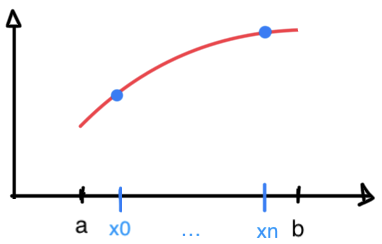
\includegraphics[width=0.5\textwidth]{immagini/GraficoAscisseInterpolazione.png}
\caption{\label{fig:GraficoAscisseInterp} Esempio delle ascisse (\ref{eq:ascisseDistinte})}
\end{figure}

\paragraph{Divagazione su $\Pi_n$:}{
$\boldsymbol{\Pi_n}$ \textbf{è lo spazio vettoriale dei polinomi di grado al più} $\boldsymbol n$. Uno spazio vettoriale è un insieme per il quale una combinazione lineare dei suoi elementi produce un elemento dello spazio stesso.
Infatti, $\forall q_1, q_2\in\Pi_n$ e $\forall \alpha,\beta\in\mathbb R$, è ottenuto che $\alpha \cdot q_1(x)+\beta\cdot q_2(x)\in\Pi_n$. $\alpha \cdot q_1(x)$ e $\beta\cdot q_2(x)$ sono moltiplicazioni che non aumentano il grado della somma, al massimo lo diminuiscono.

Se $p(x)\in\Pi_n$ è il polinomio interpolante $f(x)$, allora è possibile scriverlo come
\begin{equation}\label{eq:PolGenerico}
    p(x)=\sum_{k=0}^{n}a_kx^k.
\end{equation}
I polinomi $x^0,\, x^1,\, x^2,\, \hdots,\, x^n\in\Pi_n$ sono linearmente indipendenti e questi costituiscono la base canonica di $\Pi_n$. Pertanto, $\dim(\Pi_n)=n+1$. Questo significa che, per individuare univocamente un polinomio di $\Pi_n$,  saranno necessarie $n+1$ condizioni linearmente indipendenti.}

L'esistenza e l'unicità del polinomio interpolante è enunciata dal seguente teorema.
\begin{theorem}[Esistenza ed Unicità del polinomio interpolante]\label{th:EsisUnicPolInterp}\footnote{Slide 2 PDF 15, TH 4.1 PG 78}
    $\exists!\, p(x)\in\Pi_n: p(x_i)=f_i,\, i=0,\hdots,n$, date le coppie di dati $(x_i,f_i),\; i=0,\hdots,n$, soddisfacenti (\ref{eq:ascisseDistinte}).
\end{theorem}
\begin{proof}
    Considerato il polinomio incognito in forma (\ref{eq:PolGenerico}) ed imposte le \underline{condizioni di interpolazione (\ref{eq:condInterp})}:
    \begin{equation}\label{eq:InterpEqLin}
        p(x_i)\equiv\sum_{k=0}^{n}a_kx_i^k=f_i,\quad i=0,\hdots,n.
    \end{equation}
    Questo è un sistema di equazioni lineari $(n+1)$, nelle $n+1$ incognite $a_0,\hdots,a_n$. Il sistema può essere denotato in forma vettoriale come
    \begin{equation}\label{eq:sistemaVand}
        V\underline{a}=\underline{b},
    \end{equation}
    dove
    \begin{equation*}
        \underline{a} = 
    \begin{bmatrix}
        a_0\\
        a_1\\
        \vdots\\
        a_n
    \end{bmatrix},\; \underline{b}=
    \begin{bmatrix}
        f_0\\
        f_1\\
        \vdots\\
        f_n
    \end{bmatrix}\in\mathbb R^{n+1},\;
    V=\begin{bmatrix}
        x_0^0 & x_0^1 & \hdots & x_0^n\\
        x_1^0 & x_1^1 & \hdots & x_1^n\\
        \vdots & \vdots &\ddots & \vdots\\
        x_n^0 & x_n^1 & \hdots & x_n^n
    \end{bmatrix}\in\mathbb R^{(n+1)\times (n+1)}.
    \end{equation*}
    $V$ è la matrice dei coefficienti, definita univicomente dalle ascisse, e trasposta di una matrice di Vandermonde.

    \begin{definition}[Matrice di Vandermonde]
        Una matrice di Vandermonde ha la caratteristica di essere definita con attraverso una progressione geormetrica, ovvero gli elementi di $V$ sono del tipo $v_{i,j}=v_i^{j-1}$.
    \end{definition}
    
    \begin{remark}
        È nota la seguente proprietà delle matrici di Vandermonde, quindi di $V$: 
        \begin{equation*}
            \det(V)\overset{\footnotemark}{=}\prod_{\underbrace{i>j}_{i\neq j}}(x_i-x_j).\footnotemark
        \end{equation*}
    \end{remark}
    \footnotetext{Produttoria di tutte le coppie di elementi ascisse $x$ con indice $i>j$. Le ascisse $x_0, \hdots, x_n$ soddisfano (\ref{eq:ascisseDistinte}).}
    
    In virtù dell'ipotesi (\ref{eq:ascisseDistinte}), segue che $\det(V)\overset{\footnotemark}{\neq} 0 \Rightarrow \exists!$ la soluzione per (\ref{eq:sistemaVand}) $\iff\exists! p(x)\in\Pi_n$ che soddisfa le condizioni di interpolazione \ref{eq:condInterp}.
\end{proof}
\footnotetext{Non nullo dato che le ascisse si interpolazione $x_0, \hdots, x_n$ sono distinte.}

Il problema discreto (\ref{eq:sistemaVand}), per la determinazione di (\ref{eq:InterpEqLin}), deriva dall'aver scelto la base delle potenze, ovvero ${x^0,x^1,\hdots, x^n}$, come base di $\Pi_n$.

\begin{definition}[Polinomio Interpolante]
    Il polinomio (\ref{eq:InterpEqLin}) è noto come \textbf{polinomio interpolante} la funzione sulle ascisse assegnate.
\end{definition}

Il calcolo del polinomio interpolante tramite la risoluzione di (\ref{eq:sistemaVand}) è inefficiente per il costo computazionale elevato e per il numero di condizionamento di $V$, il quale cresce rapidamente al crescere di $n$.

È necessario cercare un modo alternativo per il calcolo del polinomio interpolante $p(x)$, ovvero utilizzare una base diversa da quella delle potenze per il polinomio interpolante. Per questo sono definiti i polinomi della seguente Sezione, atti a calcolare il polinomio interpolante con una base diversa.

\subsection{Forma di Lagrange e di Newton}
\begin{definition}[Base di Lagrange]\footnote{Slide 7 PDF 15, PG 79.}
    La \textbf{base di Lagrange} è definita dai seguenti \textbf{polinomi di Lagrange}:
    \begin{equation}\label{eq:polLagrange}
        L_{in}=\prod_{j=0,\,j\neq i}^{n} \frac{x-x_j}{x_i-x_j},\quad i=0,1,\hdots,n, 
    \end{equation}
    dove $i$ stabilisce quale polinomio è considerato ed $n$ determina il grado del polinomio.
\end{definition}

Date le ascisse definite come (\ref{eq:ascisseDistinte}), allora i polinomi di Lagrange (\ref{eq:polLagrange}) sono ben definiti ed hanno le seguenti proprietà:
\begin{itemize}
    \item[P1)] I polinomi sono ben distinti se $x_i-x_j\neq 0\,(\rightarrow x_i\neq x_j),\; i\neq j$ \footnote{Ipotesi di (\ref{eq:ascisseDistinte}).};
    \item [P2)]\footnotemark $L_{in}(x)\in\Pi_n,\; \forall i=0,\hdots,n$;
    \footnotetext{La proprietà, il grado dei polinomi $L_{in}$, non è determinata dal denominatore di $L_{in}$, ma dal nominatore di questa. $L_{in}(x)$ è una moltiplicazione di polinomi monici di grado $n$ moltiplicati $n$ volte.}
    \item[P3)]\footnote{Dimostrazione di P2).}$L_{in}(x_k)=
   \begin{cases}
     1 & \text{se $\;k=i$ (quindi nom=denom);}\\
     \underset{\footnotemark}{0} & \text{se $\;k\neq i$.}
   \end{cases}$
    \footnotetext{$x=x_j$ in almeno una moltiplicazione, quindi è 0.}
    \item[P4)] I polinomi $\{L_{0n}(x), \hdots, L_{nn}(x)\}$ sono tra loro \uline{linearmente indipendenti}\footnotemark.
    Infatti, se
    \begin{equation*}
        \sum_{i=0}^n \alpha_i\, L_{in}(x)=0, \, \forall x \Longrightarrow \alpha_i=0,\quad i=0,\hdots,n.
    \end{equation*}
    È possibile dimostrare la tesi per un generico $k\in \{0,\hdots,n\}$ valutando $0=\sum_{i=0}^n \alpha_i\, L_{in}(x_k)=\alpha_k\,\underbrace{L_{kn}(x_k)}_{1 \text{ per P3)}}=\alpha_k.$ Pertanto, $\boldsymbol{\{\underbrace{L_{0n}(x), \hdots,L_{nn}(x)}_{n+1}\}}$ costituiscono una base per $\Pi_n$, detta \textbf{base di Lagrange}.
\end{itemize}
\footnotetext{Significa che una combinazione lineare per $p$, polinomio nullo, deve essere a coefficienti nulli.}

Un'importante conseguenza dei punti P3) e P4) è il prossimo Teorema.

\begin{theorem}[Forma di Lagrange]
    Il polinomio interpolante $p(x)\in \Pi_n$, che soddisfa le condizioni (\ref{eq:condInterp}), è dato da 
    \begin{equation}\label{eq:polInterpd}
        \boldsymbol{p(x)=\sum_{k=0}^{n}} \underset{\footnotemark}{\boldsymbol{f_k}}\, \boldsymbol{L_{kn}(x)}.
    \end{equation}\footnotetext{Coefficienti di rappresentazione del polinomio interpolante rispetto alla base interpolante.}
\end{theorem}
\begin{proof}
    Definita la funzione di Kronecker (da conoscere): 
    \begin{equation}\label{eq:formaKronecker}
        L_{in}(x_i)=\delta_{ik} = 
        \begin{cases}
            \boldsymbol 1 & i=k;\\
            \boldsymbol 0 & i\neq k.
        \end{cases}
    \end{equation}
   Quindi
   \begin{equation*}
       L_{kn}(x_i)=\delta_{ki}\Rightarrow p(x_i)=\sum_{k=0}^n f_k\, L_{kn}(x_i) = \sum_{k=0}^n f_k\, \delta_{ki} = f_i \equalto{\delta_{ii}}{1} = f_i,\quad \forall i=0,\hdots,n.
   \end{equation*}
\end{proof}

\begin{definition}
    \textbf{(\ref{eq:polInterpd})} costituisce la \textbf{forma di Lagrange} del polinomio interpolante.
\end{definition}

La precedente Definizione significa che (\ref{eq:polInterpd}) è espresso rispetto alla base di Lagrange, anche se il polinomio interpolante non varia.

\begin{algorithm}
\caption{Impementazione del polinomio interpolante nella forma di Lagrange.}\label{alg:implPolIntFormaLagr}
    \begin{lstlisting}[style=Matlab-editor]
    function y = lagrange (xi, fi, x)
    %   function y = lagrange (xi, fi, x)
    %   Implementazione del polinomio interpolante nella forma di Lagrange.
    %
    %   Input:
    %   xi  - vettore delle ascisse di interpolazione (utili per calcolare f)
    %   fi  - vettore delle immagini delle xi
    %   x   - vettore delle ascisse
    %
    %   Output:
    %   y   - vettore sui dati interpolati
    %
    if length(xi) ~= length(unique(xi)), error('ascisse non distinte'), end
    if length(xi) - length(fi) ~= 0
        error('xi e fi hanno lunghezze diverse')
    end
    n = length(xi); %grado del polinomio n-1 (in Matlab i contatori sono da 1 ad n-1);
    if n < 1, error('numero di xi e fi insufficienti'), end 
    y = zeros(size(x)); %y e' una matrice quadrata con dimensione indipendente da n;
    for i = 1 : n
        y = y + fi(i) * Lin(i, xi, x);
    end
    return
    \end{lstlisting}
\end{algorithm}

\begin{algorithm}
\caption{Impementazione della base del polinomio interpolante nella forma di Lagrange.}\label{alg:implBasePolIntFormaLagr}
    \begin{lstlisting}[style=Matlab-editor]
    function L = Lin(i, xi, x)
    %
    %   function L = Lin(i, xi, x)
    %   Lin function che calcola i-esima inversa del polinomio di Lagrange.
    %   Input:
    %   i   - indice della funzione
    %   xi  - vettore ascisse sulle quali e' calcolata f
    %   x   - stesso della function lagrange
    %
    %   Output:
    %   L   - vettore con la base ricercata
    %
    %   Non sono inclusi controlli perche' svolti nel layer superiore
    L = ones(size(x));
    zi=xi(i);
    xi(i)=[];
    n = length(xi);
    for j = 1 : n
        L = L.*(x-xi(j));
    end
    L = L / prod(zi - xi);
    return
    \end{lstlisting}
\end{algorithm}

È importante utilizzare manipolazioni vettoriali al posto di cicli, in quanto le prime sono migliori per prestazioni (oltre ad essere più compatte).

Date le $n+1$ coppie $(x_i,f_i),\; i=0,\hdots,n$, con $x_i\neq x_j$, se $i\neq j$ e $f_i\overset{\footnotemark}{\equiv} f(x_i)$,
\begin{equation*}
    \boldsymbol{\exists!p(x)\in\Pi_n:p(x_i)=f_i,\quad i=0,\hdots, n},
\end{equation*}
\footnotetext{Condizione ideale perché non è sempre vero che $f$ possa essere calcolata (nel nostro lo è possibile).}
dove $p(x)$ è il polinomio interpolante di $f(x)$ sulle ascisse assegnate.

Inoltre, è utile ribadire che le rappresentazioni del polinomio interpolante (\ref{eq:PolGenerico}) e (\ref{eq:polInterpd}) sono algebricamente uguali, quindi segue che: 
\begin{equation}\label{eq:equivBasi}
p(x)=\sum_{i=0}^n \boldsymbol{a_i}\, x^i \equiv \sum_{i=0}^n f_i\, \boldsymbol{L_{in}(x)},
\end{equation}
dove $x_i$ rappresenta la base delle potenze ed $L_{in}(x)$ la base di Lagrange.

Questa semplicità formale non si concilia con requisiti computazionali per il calcolo, in modo incrementale, del polinomio.

Il problema è capire come modificare la rappresentazione del polinomio $p(x)$ rispetto alla base utilizzata, se aggiunta un'ulteriore ascissa di interpolazione $x_{n+1}\notin\{x_0,\hdots,x_n\}$, in modo da calcolare $f_{n+1}$ (ovvero $f(x_{n+1})$). Data $\widehat{p}(x)\in\Pi_{n+1}:\widehat{p}(x_i)=f_i,\, i=0,\hdots,n+1,$ è interessante capire in che relazione sono $\widehat{p}(x)$ e $p(x)$, considerando che sono considerate due basi per i polinomi. Come visto per (\ref{eq:equivBasi}), allora
\begin{equation}
    \begin{matrix}
         \widehat{p}(x)&=&\sum_{i=0}^{n+1}\boldsymbol{\widehat{a}_i}\, x^i&\equiv&\sum_{i=0}^{n+1} f_i\, \boldsymbol{L_{i,n+1}(x)},\\
        p(x)&=&\sum_{i=0}^n a_i\,\boldsymbol{x^i}&\equiv&\sum_{i=0}^n f_i\, \boldsymbol{L_{in}(x)},
    \end{matrix}
\end{equation}
con rispettivamente $\boldsymbol{\widehat{a}_i}$ ed $\boldsymbol{L_{in+1}(x)}$, $\boldsymbol{x^i}$ ed $\boldsymbol{L_{in}(x)}$ collegate fra loro.
Le funzioni di base sono le stesse, ma i coefficienti sono diversi, sono soluzione di due sistemi lineari di dimensione diversa, con matrici di coefficienti diverse (le quali non si prestano bene alla costruzione incrementale del polinomio). 

È necessario definire una base di rappresentazione, in modo tale che $\widehat p(x)$ sia ottenuta da $p(x)$, aggiungendo una funzione di base ed il relativo coefficiente, mentre tutti gli altri rimangono gli stessi di $p(x)$. Questo è possibile utilizzando, come base di rappresentazione, i \textbf{polinomi di base di Newton}:

\begin{equation}\label{eq:polBaseNewt}
    \begin{cases}
        \omega_0(x)\equiv 1;\\
        \omega_r(x)\overset{\footnotemark}{=}(x-\overset{\footnotemark}{\boldsymbol{x_{r-1}}})\,\omega_{r-1}(x),\quad r=1,\hdots,n.
    \end{cases}
\end{equation}
\addtocounter{footnote}{-1}
\footnotetext{Moltiplicazione dell'elemento $\omega_{r-1}(x)$ per un polinomio monico; $x_{r-1}$ è la $(r-1)$-esima ascissa di interpolazione.}

\stepcounter{footnote}
\footnotetext{$(r-1)$-esima ascissa di interpolazione.}

Se gli altri coefficienti delle funzioni di base rimangono gli stessi di $p(x)$ è possibile definire il nuovo polinomio ottenendo una costruzione incrementale del polinomio interpolante.

$\omega_r$ definito in (\ref{eq:polBaseNewt}) è una relazione ricorsiva utilizzata per il calcolo, in modo efficiente, di $p(x)$ e può essere rappresentato come
\begin{equation*}
    \omega_{k+1}(x)=(x-x_k)\, w_k(x),\quad k=0,\hdots, n.
\end{equation*}
oppure è possibile scriverlo come polinomio monico, ovvero il polinomio con coefficiente del termine di grado più alto uguale ad 1, in forma esplicita come
\begin{equation}\label{polBaseNewt2}
    w_k(x)=\prod_{i=0}^{k-1}(x-x_i),\quad k=1,\hdots,n.
\end{equation}

Utilizzando il principio di induzione è possibile verificare le seguenti \textbf{proprietà di} $\omega_r$:
\begin{enumerate}
    \item $w_r(x)$ è un polinomio monico di grado $r,\; \forall r\geq 0$ (ovvero $\omega_r\in\Pi_r$);
    \item $\forall r\geq 0 \, :\, \{\underbrace{\omega_0(x), \hdots, \omega_r(x)}_{r+1}\}$ sono linaremente indipendenti \footnote{Conseguenza del punto precendete dato che i gradi sono distinti.};
    \item $\{\omega_0(x),\hdots,\omega_r(x)\}$ sono una base per $\Pi_r$ \footnote{Conseguenza del punto precedente.};
    \item $\forall r \geq 1\,:\, \boldsymbol{w_r(x)=\prod_{j=0}^{r-1}(x-x_j)}$ \footnote{Ottenuta induttivamente dalla seconda riga del sistema (\ref{eq:polBaseNewt}) con gli zeri dei polinomi conosciuti. Questa relazione ricorsiva è utilizzata per il calcolo efficiente del polinomio.};
    \item Date le ascisse distinte $x_0, \hdots, x_n$:
        $\begin{cases}
        \boldsymbol{w_r(x_j)=0}, & \boldsymbol{j\leq r-1},\\
        w_r(x_j)\neq 0, & j\geq r.
        \end{cases}$
\end{enumerate}

È possibile denotare 
\begin{equation}\label{eq:polNotaz}
    p_r(x)\in\Pi_r\, :\, p_r(x_i)=f_i,\quad i=0,\hdots, r.
\end{equation}

È possibile definire la famiglia dei polinomi $\{p_r\}_{r=0,\hdots,n}$ (dove $n$ è il grado da raggiungere), in modo incrementale, con la seguente modalità.

\begin{theorem}[Forma di Newton]\label{th:formaNewt}\footnote{Slide 5 PDF 16, TH 4.3 PG 80.}
    La famiglia di polinomi interpolanti definita in (\ref{eq:polNotaz}) è ottenuta ricorsivamente come: 
    \begin{equation}\label{eq:famPolInt}
    \begin{cases}
        p_0(x)\equiv f_0\in\Pi_0\\
        p_r(x) = p_{r-1}(x)+ f[x_0,\hdots, x_r]\,\omega_r(x),\; r=1,2,\hdots
    \end{cases}
    \end{equation}
    dove $\boldsymbol{f[x_0, \hdots, x_r]}$ è la \textbf{differenza divisa di ordine $\boldsymbol r$ della funzione $\boldsymbol f$ sulle ascisse $\boldsymbol{x_0, \hdots, x_r}$}, definita come:
    \begin{equation}\label{eq:diffDivisa}
       \boldsymbol{f[x_0, \hdots, x_r] \overset{\text{def.}}{=} \sum_{i=0}^r\frac{f_i}{\prod_{j=0, j\neq i}^{r}(x_i-x_j)}}.
    \end{equation}
\end{theorem}
\begin{proof}\footnote{Dimostrazione riscorsiva del sistema (\ref{eq:famPolInt}) e di (\ref{eq:diffDivisa}).}
    Per induzione la tesi è vera, con $r=0$, poiché $p_0(x)\equiv f_0\equiv f[x_0]$. Supposto vero per $r-1$ sarà dimostrato per $r$.
    
    Per ipotesi è supposto che
    \begin{equation*}
        p_{r-1}(x)\in\Pi_{r-1}:\boldsymbol{p_{r-1}(x_i)=f_i,\; i=0,\hdots r-1}
    \end{equation*}
    e che $p(x)$ sia definto come in (\ref{eq:famPolInt}). Sarà dimostrato quanto segue:
    \begin{enumerate}
        \item $p_r(x_i)=f_i, \; i=0,\hdots,r$ \footnotemark;
        \item $f[x_0, \hdots, x_r]$ è definita come in (\ref{eq:diffDivisa}).
    \end{enumerate}
\footnotetext{Quindi è necessario dimostrare che $p_r$ è calcolabile come $p_{r-1}$.}
    \begin{proof}[Dimostrazione di 1.]
        \begin{equation*}
        \forall i=0,\hdots, r-1:\; p_r(x_i)=\underbrace{p_{r-1}(x_i)}_{f_i}+\underbrace{f[x_0, \hdots, x_r]}_{\footnotemark}\underbrace{\omega_r(x_i)}_{0}=f_i.
        \end{equation*}
        Per $i=r$, essendo le ascisse distinte, $\omega_r(x_r)\neq 0$ ed imponendo $p_r(x_r)=p_{r-1}(x_r)+f[x_0,\hdots,x_r]\,\omega_r(x_r)=f_r$ è ricavato che
        \footnotetext{Non è definito.}
        \begin{equation}\label{eq:ridefDifDivisa}
            f[x_0, \hdots, x_r]\overset{\text{def}}{=}\frac{f_r-p_{r-1}(x_r)}{\omega_r(x_r)},
        \end{equation}
        che è ben definito essendo  $\omega_r(x_r)\neq 0$.
        È necessario dimostrare che la differenza divisa espressa come (\ref{eq:ridefDifDivisa}) coincide con (\ref{eq:diffDivisa}). A questo fine è possibile osservare che $f[x_0, \hdots, x_r]$ è il coefficiente principale di $p_r(x)$.
        È definito l'algoritmo per la soluzione in due passi: 
        \begin{enumerate}
            \item scrittura di $p_r(x)$ in forma di Lagrange;
            \item calcolo del coefficiente principale di $p_r(x)$ in forma di Lagrange.
        \end{enumerate}
        Quindi i due coefficienti dovranno coincidere, per il principio di identità dei polinomi.
    
        La forma di Lagrange di $p_r(x)$ è espressa come segue:
        \begin{equation*}
            \begin{matrix}
                p_r(x) &=& \sum_{i=0}^r f_i\, \boldsymbol{L_{ir}(x)} \\
                &\overset{\footnotemark}{=}& \sum_{i=0}^r f_i\,\boldsymbol{\prod_{j=0, j\neq i}^r\frac{x-x_j}{x_i-x_j}} \\
                &=&\sum_{i=0}^r \frac{f_i}{\prod_{j=0, j\neq i}^r(x_i-x_j)}\cdot \underset{\footnotemark}{\boldsymbol{\prod_{j=0, j\neq i}^r(x-x_j)}} \\
                &\overset{\footnotemark}{=}& x^r\boldsymbol{\sum_{i=0}^r\frac{f_i}{\prod_{j=0, j\neq i}^r(x_i-x_j)}}\;+ \text{ (termini di ordine inferiore in $x$) }\\
                &\overset{\footnotemark}{\equiv}& x^r\, \boldsymbol{f[x_0,\hdots, x_r]}\; + \text{ (termini di ordine inferiore in $x$) }.
            \end{matrix}
        \end{equation*}
    \end{proof}
    \addtocounter{footnote}{-3}
    \footnotetext{Scittura del polinomio di Lagrange di grado $r$ in forma esplicita ($r\rightarrow n)$.}
    
    \stepcounter{footnote}
    \footnotetext{$\prod_{j=0,\\j\neq i}^r (x-x_j)$ è un polinomio monico di grado $r$, è una produttoria di $r$ polinomi di grado 1.}
    
    \stepcounter{footnote}
    \footnotetext{Forma di Lagrange.}
    
    \stepcounter{footnote}
    \footnotetext{Forma diversa da Lagrange.}
    Da questo è possibile concludere che la (\ref{eq:diffDivisa}) vale.

    \begin{proof}[Dimostrazione 2.]
        La seconda parte della dimostrazione del Teorema è svolta come dimostrazione del punto P5), esposto fra poco.
    \end{proof}
\end{proof}

\begin{remark}[Forma di Newton del polinomio interpolante]\label{rem:formaNewton}\footnote{Slide 8 PDF 16.}
    Sia $p(x)\in\Pi_n$, polinomio interpolante $f(x)$ sulle ascisse $\{x_0,\hdots, x_n\}$, $p(x)$ coincide con $p_n(x)$ in (\ref{eq:polNotaz}).
    Per induzione è ottenuta la \textbf{forma di Newton del polinomio interpolante}: 
    \begin{equation}\label{eq:polInterNewt}
        \boldsymbol{p(x)\equiv p_n(x) = \sum_{i=0}^{n} f[\underbrace{x_0,\hdots, x_i}_{i+1}]\,\omega_i(x)},
    \end{equation}
    dove $\omega_i(x)$ è la dunzione di base.
\end{remark}

\paragraph{\ul{N.B.}:} \textbf{La forma di Lagrange e la forma di Newton di $p(x)$ definiscono lo stesso polinomio interpolante}, il quale esiste ed è unico, se le ascisse di interpolazione sono tra loro distinte. Ciò significa che per $p(x)$ varia solo la sua rappresentazione. Questo ha il pregio di prestarsi alla costruzione incrementale del polinomio aggiornandosi in modo dinamico.

\paragraph{Esempio di caso d'uso polinomio interpolante:} se fosse richiesto di approssimare ciò che è sotto una certa curva questa viene calcolata con un numero prefissato di punti, poi se ne sono aggiungono uno ad uno fino a che non è più possibile effetturare una stima accurata.

La definizione in forma di Newton di $p(x)$ come (\ref{eq:polInterNewt}) permette di ottenere funzioni di base in funzione delle precedenti. Pertanto, questo non permette di calcolare la differenza divisa e la rappresentazione $f[x_0,\hdots, x_r]$ non è algoritmicamente preferibile. Per arrivare al fine di ottenere un algoritmo efficiente, sono esaminate alcune proprietà delle differenze divise.

\paragraph{\underline{Proprietà differenze divise (\ref{eq:diffDivisa})}:} \footnote{Slide 9-11 PDF 16, TH 4.4 PG 82.}
\begin{itemize}
    \item[P1)](Linearità dell'operatore) Se $f$ e $g$ sono funzioni in variabili reali $\alpha,\,\beta \in\mathbb R$, allora
    \begin{equation*}
        (\alpha\cdot f + \beta\cdot g)[x_0,\hdots, x_r]=\alpha\cdot f[x_0,\hdots, x_r]+\beta\cdot g[x_0,\hdots, x_r];
    \end{equation*}
    \item[P2)](Simmetria dell'operatore) Se $\{i_0,\hdots,i_r\}$ è una permutazione di $\{0,\hdots, r\}$, allora:
    \begin{equation*}
        f[x_0,\hdots,x_r]=f[x_{i_0},\hdots,x_{i_r}];
    \end{equation*}
    \item[P3)] Se $f(x)=\sum_{i=0}^ka_ix^i$, allora $f[x_0,\hdots, x_r]=
    \begin{cases}
        a_k,\; r=k;\\
        0,\; r>k.
    \end{cases}$
    \footnote{Sia $g(x)\in\Pi_n$, allora il polinomio $p(x)\in\Pi_n$ che interpola $g(x)$ sulle ascisse distinte $x_0,\hdots,x_n$ è $g(x)$ stesso ($p(x)=g(x)$), per l'unicità del polinomio interpolante.
    Il polinomio $p(x)\in\Pi_r,$ con $r>n$, che interpola $g(x)$ sulle $r+1$ ascisse distinte $x_0, \hdots, x_r$, è sempre $g(x)$ per lo stesso motivo.}

    \item[P4)] Se $f\in C^{(\boldsymbol r)}[a,b],\, a=\underset{i=0,\hdots,\boldsymbol r}{\min}x_i,\, b=\underset{i=0,\hdots,\boldsymbol r}{\max}x_0$, allora
    \begin{equation}\label{eq:P4DiffDiv}
        f[x_0,\hdots, x_{\boldsymbol r}]=\frac{f^{(\boldsymbol r)}(\xi)}{\boldsymbol r!},\; \xi\in [a,b],
    \end{equation}

    dove $[a,b]$ è il più piccolo intervallo che contiene le ascisse di interpolazione. Questa proprietà vale anche nel caso in cui 2 o più ascisse coincidano. In questo caso, la definizione di differenza divisa vale come limite.

    \item[P5)] \begin{equation}\label{eq:P5DiffDiv}
        f[\underbrace{x_0,\hdots,x_r}_{r+1}]=\frac{f[\overbrace{x_1,\hdots,x_r}^{r}]-f[\overbrace{x_0,\hdots,x_{r-1}}^{r}]}{x_r-x_0}.\footnotemark
    \end{equation}
    \footnotetext{Le due differenze divise al nominatore differiscono solo per l'ascissa $x_0$. Il concetto è che, se è applicata iterativamente questa proprietà, allora è possibile scrivere le differenze divise come combinazione di differenze divise, con $r-1$ argomenti, fino ad ottenere un solo argomento. Quando l'argomento è unico allora la differenza divisa coinciderà con il valore calcolato nell'argomento.}
\end{itemize}

(\ref{eq:P5DiffDiv}) è  una proprietà algoritmica importante, è utilizzata per il calcolo efficiente della differenze divisa ed è possibile dimostrarla come segue.

\begin{proof}[Dimostrazione P5)] \footnote{Tramite la definizione di differenza divisa. Sono calcolate due differenze divise, è effettuata la somma ed è ottenuta l'espressione ricercata.}
    \begin{equation}\label{eq:dimPropDiffDiv}
        \begin{matrix}
            \frac{1}{x_r-x_0}(f[x_1,\hdots, x_r]-f[x_0,\hdots,x_{r-1}]) = \frac{1}{x_r-x_0}\left(\sum_{k=1}^r\frac{f_k}{\prod_{j=1,j\neq k}^r(x_k-x_j)}-\sum_{k=0}^{r-1}\frac{f_k}{\prod_{j=0,j\neq k}^{r-1}(x_k-x_j)}\right)\\
            = \frac{1}{x_r-x_0}\,\left(\underbrace{\overbrace{\frac{f_r}{\prod_{j=1,j\neq r}^r(x_r-x_j)}}^{(a)}-\overbrace{\frac{f_0}{\prod_{j=0,j\neq 0\rightarrow j=1}^{r-1}(x_0-x_j)}}^{(b)}}_{\text{Elementi comuni alle due sommatorie}}+\underbrace{\sum_{k=1}^{r-1}f_k\,\left(\frac{1}{\prod_{j=1,j\neq k}^r(x_k-x_j)}-\frac{1}{\prod_{j=0,j\neq k}^{r-1}(x_k-x_j)}\right)}_{\underset{\footnotemark}{(c)}}\right)\\
             =(a)+(b)+(c),
        \end{matrix}
    \end{equation}
    \footnotetext{Dato che gli indici da 1 ad $r-1$ sono comuni ad entrambe le produttorie, saranno raggruppati gli addendi con indici comuni e lasciati gli addendi non comuni. Addendi con indice uguale ad $r$ sono sommatorie, con indice uguale a 0 sono la somma $a+b$.}
    dove $\frac{1}{x_r-x_0}$ è inglobata in $(a),(b)$ e $(c)$ come segue:
    \begin{equation*} 
        \begin{matrix}
        (a) = \frac{1}{x_r-x_0}\frac{f_r}{\prod_{j=1,j\neq r}^r(x_r-x_j)}\overset{\footnotemark}{=}\frac{f_r}{\prod_{j=0,j\neq r}^r(x_r-x_j)};\\
        (b) = \frac{1}{x_0-x_r}=\frac{f_0}{\prod_{j=0,j\neq 0}^{r-1}(x_0-x_j)}=\frac{f_0}{\prod_{j=0,j\neq 0}^r(x_0-x_j)};\\
        (c) = \frac{1}{x_r-x_0}\sum_{k=1}^{r-1}\frac{f_k}{\prod_{j=1,j\neq k}^{r-1}(x_k-x_j)}\underbrace{\left(\frac{1}{x_k-x_r}-\frac{1}{x_k-x_0}\right)}_{\footnotemark}=
        \frac{1}{\cancel{x_r-x_0}}\sum_{k=1}^{r-1}\frac{f_k}{\prod_{j=1,j\neq k}^{r-1}(x_k-x_j)}\left(\frac{\cancel{x_k}-\cancel{x_0}-\cancel{x_k}+\cancel{x_r}}{(x_k-x_r)(x_k-x_0)}\right)=\\
        \sum_{k=1}^{r-1}\frac{f_k}{\prod_{j=0,j\neq k}^{r-1}(x_k-x_j)};
        \end{matrix}
    \end{equation*}
    \addtocounter{footnote}{-1}
    \footnotetext{Ultimo termine della sommatoria della differenza divisa delle ascisse $x_0,\hdots,x_r$.}
    \stepcounter{footnote}
    \footnotetext{Termini necessari per le caratteristiche degli indici.}
    
    Pertanto, unendo i precedenti risultati:
    \begin{equation*}
        \textbf{(\ref{eq:dimPropDiffDiv})}=\sum_{k=0}^r\frac{f_k}{\prod_{j=0,j\neq k}^r (x_k-x_j)}\overset{\footnotemark}{=} f[x_0,x_1,\hdots,x_r].
    \end{equation*}
    \footnotetext{Ovvero ciò che è necessario dimostrare.}
\end{proof}

\paragraph{Esempio di utilizzo della proprietà (\ref{eq:P5DiffDiv}):} Considerando il caso $\boldsymbol{n=3}$:
\begin{equation*}
    \boldsymbol{p(x)=f[x_0]\;\equalto{\omega_0(x)}{1}+f[x_0,x_1]\omega_1(x)+f[x_0,x_1,x_2]\omega_2(x)+f[x_0,x_1,x_2,x_3]\omega_3(x)},
\end{equation*}
allora è possibile generalizzarlo in la seguente tabella triangolare:
 
\begin{center}
\begin{tabular}{|c|c|c|c|c|} 
\hline
 & $\overset{\footnotemark}{0}$ & $\overset{\footnotemark}{1}$ & 2 & 3 \\
\hline
$x_0$ & $\boldsymbol{f_0 = f[x_0]}$ & & &  \\ 
$x_1$ & $f_1 = f[x_1]$ & $\boldsymbol{f[x_0,x_1]}$ & &  \\ 
$x_2$ & $f_2 = f[x_2]$ & $f[x_1,x_2]$ &$ \boldsymbol{f[x_0,x_1,x_2]}$ & \\
$x_3$ & $f_3 = f[x_3]$ & $f[x_2, x_3]$ & $f[x_1,x_2,x_3]$ & $\boldsymbol{f[x_0,x_1,x_2,x_3]}$ \\
\hline
\end{tabular}
\end{center}
\addtocounter{footnote}{-1}
\footnotetext{Differenza tra l'indice delle ascisse (utillizzata la proprietà incementale delle differenze divise).}

\stepcounter{footnote}
\footnotetext{Differenze divise su due ascisse.}

Gli elementi sulla diagonale principale, ovvero quelli in grassetto, sono i coefficienti del polinomio interpolante nella forma di Newton (\ref{eq:polInterNewt}).

La tabella è calcolata dal basso verso l'alto per evitare di memorizzare tutti i dati della tabella. Non è necessario memorizzarla tutta perché è possibile sovrascrivere gli elementi a sinistra con quelli a destra (quindi in fine saranno presenti le differenze divise in grassetto). Per questo è necessario calcolare prima la colonna 0 e poi la 1, 2 e 3 sovrascrivendone, via via, gli elementi. Quanto appena scritto non è valido se gli elementi sono calcolati dall'alto verso il basso.

Utilizzando il metodo di calcolo più conveniente è possibile utilizzare due vettori: uno per le ascisse di interpolazione $(x_0,\hdots, x_3)$ ed uno per i dati del problema da sovrascrivere con i coefficienti dei polinomi.

La tabella ha complessità quadratica, come la forma di Lagrange, e minore rispetto a risolvere il sistema lineare con la matrice di Vandermonde (la quale ha complessità $\frac{2}{3}n^3$).

Le colonne della precedente tabella, dalla 1 alla 3, sono determinate (calcolate) dal basso verso l'alto come segue:

\begin{equation*}
    \begin{matrix}
        \underset{\footnotemark}{\boldsymbol 1}
    \begin{cases}
        f[x_2,x_3]=\frac{f[x_3]-f[x_2]}{x_{\boldsymbol 3}-x_{\boldsymbol 2}}\\
        f[x_1,x_2]=\frac{f[x_2]-f[x_1]}{x_{\boldsymbol 2}-x_{\boldsymbol 1}}\\
        f[x_0,x_1]=\frac{f[x_1]-f[x_0]}{x_{\boldsymbol 1}-x_{\boldsymbol 0}}
    \end{cases}\\
    \boldsymbol{2}\begin{cases}
        f[x_1,x_2,x_3]=\frac{f[x_{\boldsymbol 2},x_3]-f[x_1,x_{\boldsymbol 2}]}{x_{\boldsymbol 3}-x_{\boldsymbol 1}}\\
        f[x_0,x_1,x_2]=\frac{f[x_{\boldsymbol 1},x_2]-f[x_0,x_{\boldsymbol 1}]}{x_{\boldsymbol 2}-x_{\boldsymbol 0}}
    \end{cases}\\
    \boldsymbol{3}\begin{cases}
        f[x_0,x_1,x_2,x_3]=\frac{f[\boldsymbol{x_1,x_2},x_3]-f[x_0,\boldsymbol{x_1,x_2}]}{x_{\boldsymbol 3}-x_{\boldsymbol 0}}
    \end{cases}
    \end{matrix}
\end{equation*}
\footnotetext{Differiscono di un'ascissa non comune.}

È possibile notare che al denominatore le ascisse di iterpolazione differiscono rispettivamente, dall'alto al basso, di un indice 1, 2 e 3 e che tali ascisse non sono comuni alle differenze divise al denominatore delle rispettive frazioni.

\begin{remark}\footnote{Slide 6 PDF 17.}
    Nel caso generale, la precedente tabella arriverà fino a colonna $n$ (l'indice partirà da 0) ed avrà struttura analoga.
\end{remark}

\begin{algorithm}
\caption{Calcolo delle differenze divise.}\label{alg:calcDiffDiv}
    \begin{lstlisting}[style=Matlab-editor]
        % x - ascisse di interpolazione
        % f - valori della funzione nelle ascisse
        % x ed f sono vettori di dimensione n+1 perche' Matlab utilizza indici che partono da 1
        n = length(x)-1; % grado del polinomio
        for j = 1 : n
            for i = n+1 : -1 : j+1
                f(i)=(f(i)-f(i-1))/(x(i)-x(i-j)); %saranno modificati in colonna j gli elementi che vanno dall'ultimo al j+1-esimo. Il j-esimo contiente la differenza divisa, la quale e' calcolata nella riga della nota
            end
        end
    \end{lstlisting}
\end{algorithm}

\begin{remark} Il \textbf{costo computazionale} dell'\textbf{Algoritmo (\ref{alg:calcDiffDiv}}) è
    \begin{itemize}
        \item $\sum_{j=1}^{n}3(n-j+1)\overset{\footnotemark}{=} 3\sum_{j=1}^{n}j=3\cdot\frac{n(n+1)}{2}\boldsymbol{\approx \frac{3}{2}n^2\; flops}$; \footnotetext{Somma naturale.}
        \item \textbf{2 vettori} $\boldsymbol{(x, f)}$ ($x$ memorizza le ascisse interpolanti ed $f$ le differenze divise);
    \end{itemize}
\end{remark}

\noindent\textbf{Problema:} È necessario considerare il calcolo efficiente del polinomio di Newton. Del polinomio sono noti i coefficienti ed è necessario calcolare la sommatoria. Sarà utilizzata la proprietà ricorsiva del polinomio di Newton. Al fine del calcolo efficiente del polinomio di Newton è valutato un problema più semplice rispetto alla base delle potenze, il calcolo del polinomio (\ref{eq:PolGenerico})  $\left(p(x)=\sum_{k=0}^{n}a_kx^k\right)$.

Partendo da un caso semplice, ovvero con $n=3$:
\begin{equation*}
    p(x)=a_0+a_1\,x+a_2\,x^2+a_3\,x^3\overset{\footnotemark}{=} a_0+ x(a_1+x(a_2+x\,a_3)).
\end{equation*}\footnotetext{Raggruppamento.}

Supposto di avere il vettore $a=[\underbrace{\overbrace{a_0\; a_1\; \hdots\; a_n}^{n+1\text{ elementi}}}_{\footnotemark}]$ \footnotetext{In Matlab è necessario rappresentarli come $a(1)\; a(2)\,\hdots\, a(n+1)$.} è possibile calcolare il polinomio tramite l'Algoritmo \ref{alg:polHorn}.

\begin{algorithm}
\caption{Algoritmo di Horner per il calcolo di un polinomio.}\label{alg:polHorn}
    \begin{lstlisting}[style=Matlab-editor]
        p = a(n+1); % al termine dell'algoritmo conterra' il valore del polinomio
        for i = n : -1 : 1
            p = p .* x + a(i);
        end
    \end{lstlisting}
\end{algorithm}

\begin{remark}[Costo dell'Algoritmo \ref{alg:polHorn}]
    Il costo dell'algoritmo è $2n\, flops$ (\underline{per componente di $x$}).
\end{remark}

L'Algoritmo \ref{alg:polHorn} (di Horner) ha un costo minimale: sono svolte due operazioni algebriche elementari per calcolare il vettore $p(x)$, per iterazione. È, inoltre, importante osservare che questo algoritmo si presta ad essere vettorizzato in Matlab, attraverso la moltiplicazione vettoriale .*, dove $x$, in riga 3 dell'Algoritmo \ref{alg:polHorn}, può essere di qualsivolglia forma (vettore, elemento singolo, matrice). Utilizzare le capacità vettoriali di Matlab rende più efficiente il codice (quindi è necessario utilizzarlo nell'elaborato).

Inoltre, è possibile generalizzare la differenza divisa al caso della base di Newton attraverso l'algoritmo di Horner generalizzato (Algoritmo \ref{alg:polHornMod}).

\begin{example}
    Con $n=3$:
    \begin{equation*}
        \begin{matrix}
            p(x) &\overset{\footnotemark}{=}& f[x_0] + f[x_0,x_1]\,\omega_1(x) + f[x_0,x_1,x_2]\,\omega_2(x) + f[x_0,x_1,x_2,x_3]\,\omega_3(x)\\
            &\overset{\footnotemark}{=}& f[x_0]+f[x_0,x_1](x-x_0)+f[x_0,x_1,x_2](x-x_0)(x-x_1)+f[x_0,x_1,x_2,x_3](x-x_0)(x-x_1)(x-x_2)\\
            &=&\left(\left(f[x_0,x_1,x_2,x_3](x-x_2) + f[x_0,x_1,x_2]\right)(x-x_1)+f[x_0,x_1]\right)(x-x_0)+f[x_0].
        \end{matrix}
    \end{equation*}
    \addtocounter{footnote}{-1}
    \footnotetext{È noto come calcolare le defferenze divise (ovvero i coefficienti).}
    \stepcounter{footnote}
    \footnotetext{Scrittura di $\omega_i(x)$ (polinomio di Newton) in forma estesa in modo da appurare efficientemente il valore in un punto, o in più di uno. La forma estesa è la forma in cui i polinomi in base di Newton sono usati perché la loro espressione è nota.}
\end{example}

\begin{algorithm}
\caption{Algoritmo di Horner generalizzato (per il calcolo di un polinomio).}\label{alg:polHornMod}
    \begin{lstlisting}[style=Matlab-editor]
        % f(1), ..., f(n+1)   - calcolato dal codice precedente per le differenze divise
        % x(1), ..., x(n+1)   - contiene le ascisse di interpolazione
        p = f(n+1) 
        for i = n : -1 : 1
            p = p .* (x - x(i)) + f(i)
        end
    \end{lstlisting}
\end{algorithm}

\begin{remark}
    L'operazione .* in riga 5 dell'Algoritmo \ref{alg:polHornMod} è vettorizzabile.
\end{remark}

\begin{remark}[Costo dell'Algoritmo \ref{alg:polHornMod}]
    Il costo dell'algoritmo è $3n$ flops per componente.
\end{remark}

\paragraph{Intermezzo per la definizione della "Interpolazione di Hermite"}\footnote{Slides 1-3 PDF 18.} Dato il polinomio interpolante in forma di Newton (\ref{eq:polInterNewt}) allora è possibile utilizzare l'Algoritmo \ref{alg:calcP(x)} per calcolare $p(x)$.

\begin{algorithm}\caption{Pseudo-codice calcolo $p(x)$.}\label{alg:calcP(x)}
    \begin{algorithmic}
        \State $w_0\equiv 1$
        \State $p = 0$
        \For{i = 0 : n}
            \State $p = p + \omega_i * a_i$
            \State $\omega_{i+1} = \omega_i *(x - x_i)$
        \EndFor
    \end{algorithmic}
\end{algorithm}

L'Algoritmo \ref{alg:calcP(x)} utilizza il fatto che le funzioni di base possano essere ottenute in modo iterativo, moltiplicando un termine di grado uno (il polinomio monico). Pertanto, è meno efficiente dell'Algoritmo (di Horner generalizzato) \ref{alg:polHornMod} in quanto effettua $4n\, flops$ ed utilizza una variabile di appoggio ($\omega$, la quale rappresenta $\omega_0,\,\omega_1,\,\omega_{i+1}$).

Tuttavia, l'Algoritmo \ref{alg:calcP(x)} si presta facilmente per derivare un algoritmo per il calcolo della derivata prima di $p(x)$, la quale sarà significativa per gli argomenti che saranno trattati, ovvero:
\begin{equation*}
    \boldsymbol{p'(x)}=\sum_{i=0}^n\underset{\text{coeff.}}{a_i}\,\boldsymbol{\omega'_i(x)}=\sum_{\underset{\footnotemark}{i=1}}^na_i\,\boldsymbol{\omega'_i(x)}.
\end{equation*}
\footnotetext{Trasformazione in $i=1$ perché $\omega_0\equiv 1$ (vedere (\ref{eq:polBaseNewt})).}

L'obbiettivo è derivare un algoritmo per il calcolo delle derivate $\omega'(x)$ e $p'(x)$. Ciò significa che le righe precedenti si riducono a derivare un algoritmo, relativamente efficiente, per il calcolo delle derivate prime dei polinomi di base di Newton.

È possibile osservare che il calcolo di $\omega_i(x)$ come
\begin{equation*}
    \omega_i(x)=\prod_{k=0}^{i-1}(x-x_k)\Rightarrow \omega'_i(x)=\sum_{k=0}^{i-1}\prod_{j=0,j\neq k}^{i-1}(x-x_j)
\end{equation*}
è dispendioso e poco efficiente, se calcolato in questo modo.

\begin{example}
    $\omega_2(x)=(x-x_0)(x-x_1) \rightarrow \omega'_2(x)=(x-x_0)+(x-x_1)$.
\end{example}

\begin{remark}
    È possibile ottenere i polinomi, in modo ricorsivo, dall'Algoritmo \ref{alg:calcP'(x)} (ultima riga del for), ovvero:
    \begin{equation*}
        \begin{cases}
            \omega_0(x)\equiv 1,\, \omega'_0(x)\equiv 0,\\
            i\geq 1\,:\, \omega'_i(x)=\frac{\partial f}{\partial x}[\omega_{i-1}(x)(x-x_{i-1})] = \omega'_{i-1}(x)(x-x_{i-1})+\omega_{i-1}(x).
        \end{cases}
    \end{equation*}
\end{remark}

Questa osservazione porta alla definizione dell'Algoritmo \ref{alg:calcP'(x)} (dove $\omega_i$ rimane una variabile). L'algoritmo utilizza una variabile per la derivata, $\omega'_i$, ed una per il polinomio di base, $p'_i$. Pertanto, dato un polinomio, espresso con base di Newton, è noto come calcolarlo e con esso la sua derivata prima.

\begin{algorithm}\caption{Algoritmo calcolo $p'(x)$.}\label{alg:calcP'(x)}
    \begin{algorithmic}
        \State $w_0=1,\, \omega'_0=0,\, p'=0$
        \For{$i=1:n$}
            \State $\omega'_i=\omega'_{i-1}+\omega'_{i-1}\cdot (x-x_{i-1})$
            \State $\omega_i=\omega_{i-1}\cdot(x-x_{i-1})$
            \State $p'=p'+a_i\cdot\omega'_i$
        \EndFor
    \end{algorithmic}
\end{algorithm}

\subsection{Interpolazione di Hermite}\footnote{Slide 4-11 PDF 18, PG 84-86.}
[Problema:] Supposto di avere un polinomio interpolante una funzione su un numero pari ($2n+2$) di ascisse, quest'ultime sono numerate come segue:
\begin{equation}
    a\leq\overbrace{x_0 < x_{\frac{1}{2}} < x_1 < x_{\frac{3}{2}} < \hdots < x_n < x_{n+\frac{1}{2}}}^{2n+2\text{ ascisse}}\leq b.
\end{equation}

Pertanto, sotto la precedente ipotesi di ascisse distinte, $\boldsymbol{\exists!\, p(x)}\in\Pi_{\boldsymbol{2n+1}}$ (condizione importante) tale che le condizioni del polinomio interpolante (\ref{eq:condInterp}) diventano le seguenti:
\begin{equation}\label{eq:hermCondPolInterp}
    \begin{rcases}
        \boldsymbol{p(x_i)=f(x_i)}\\
        \boxed{p\left(x_{i+\frac{1}{2}}\right)=f\left(x_{i+\frac{1}{2}}\right)}
    \end{rcases} i=0,\hdots,n.
\end{equation}

Se $\forall i=0,\hdots,n: x_{i+\frac{1}{2}}\rightarrow x_i$, le ascisse che sono tra due interi, quelle con indice frazionario (ovvero $i+\frac{1}{2}$), sono fatte tendere all'ascissa a sinistra, quindi la condizione di interpolazione è duplicata. Per evitare la duplicazione è possibile riscrivere le condizioni di interpolazione (\ref{eq:hermCondPolInterp}), in modo equivalente, come:
\begin{equation}\label{eq:hermCondPolInterpMod}
    \begin{rcases}
        \boldsymbol{p(x_i)=f(x_i})\\
        \boxed{\frac{p\left(x_{i+\frac{1}{2}}\right)-p(x_i)}{x_{i+\frac{1}{2}}-x_i}=\frac{f\left(x_{i+\frac{1}{2}}\right)-f(x_i)}{x_{i+\frac{1}{2}}-x_i}}
     \end{rcases} i=0,\hdots,n,
\end{equation}
per
\begin{equation*}
    x_{i+\frac{1}{2}}\rightarrow x_i:
    \begin{cases}
        \frac{p\left(x_{i+\frac{1}{2}}\right)-p(x_i)}{x_{i+\frac{1}{2}}-x_i}\rightarrow p'(x_i)\\
        & i=0,\hdots, n.\\
        \frac{f\left(x_{i+\frac{1}{2}}\right)-f(x_i)}{x_{i+\frac{1}{2}}-x_i}\rightarrow f'(x_i)
    \end{cases}
\end{equation*}

\begin{remark}
    La seconda condizione di (\ref{eq:hermCondPolInterp}) è stata modificata nella seconda condizione di (\ref{eq:hermCondPolInterpMod}), sottraendo la prima condizione alla seconda di (\ref{eq:hermCondPolInterp}) e dividendo membro a membro per $x_{i+\frac{1}{2}}-x_i$.
\end{remark}

Data $f(x)\in C^{(1)}$ è possibile ottenere ciò che segue (vedere (\ref{eq:P4DiffDiv})):
\begin{equation}\label{eq:equivApproxf'}
    \frac{f\left(x_{i+\frac{1}{2}}\right)-f(x_i)}{x_{i+\frac{1}{2}}-x_i}=f\left[x_i,x_{i+\frac{1}{2}}\right]\rightarrow f[x_i,x_i]\equiv f'(x_i),\; i=0,\hdots,n.
\end{equation}

È possibile concludere che se $x_{i+\frac{1}{2}}\rightarrow x_i,\, \forall i=\underbrace{0,\hdots, n}_{\footnotemark}\Rightarrow\exists! p_{\boldsymbol H}(x)\in\Pi_{\boldsymbol{2n+1}}$ tale che: \footnotetext{Quindi le ascisse sono $n+1$.}
\begin{equation}\label{eq:polInterHer}
    \footnotemark\begin{cases}
        p_{\boldsymbol H}(x_i)=f(x_i)\\
        p_{\boldsymbol H}'(x_i)=f'(x_i)
    \end{cases} i=\boldsymbol{0,\hdots,n}.
\end{equation}\footnotetext{Condizioni su polinomio e sulla sua derivata prima.}

\begin{definition}[Polinomio interpolante di Hermite]
    $p_{\boldsymbol H}(x)$ è il polinomio interpolante di Hermite.  
\end{definition}

Pertanto, date le $n+1$ ascisse distinte (\ref{eq:ascisseDistinte}), $\exists!\, p_{\boldsymbol H}(x)\in\Pi_{2n+1}$, che soddisa le condizioni di interpolazione (\ref{eq:polInterHer}). Il polinomio $p_H(x)$ interpola la funzione $f(x)$ e la sua derivata, $f'(x)$, nelle ascisse di interpolazione.

\begin{example}\footnote{Slide 5 PDF 18.}
    Considerate le ascisse $x_i=i\cdot\pi,\; i=0,1,2$ e considerando la funzione
    \begin{equation*}
        f(x)=\sin(x)\overset{\footnotemark}{\Rightarrow}f'(x)=\cos(x).
    \end{equation*}
    Spiegazione grafica dell'esempio in Figura \ref{fig:PolHermite} e \ref{fig:PolHermite1}. \footnotetext{Il polinomio interpolante classico è il polinomio costante 0 perché interpola $f(x)$ nelle 3 ascisse di interpolazione. Il polinomio di Hermite interpola anche la deriva prima, ciò rende l'approssimazione più accurata rispetto a quella del polinomio classico.}
\end{example}

\begin{figure}
\centering
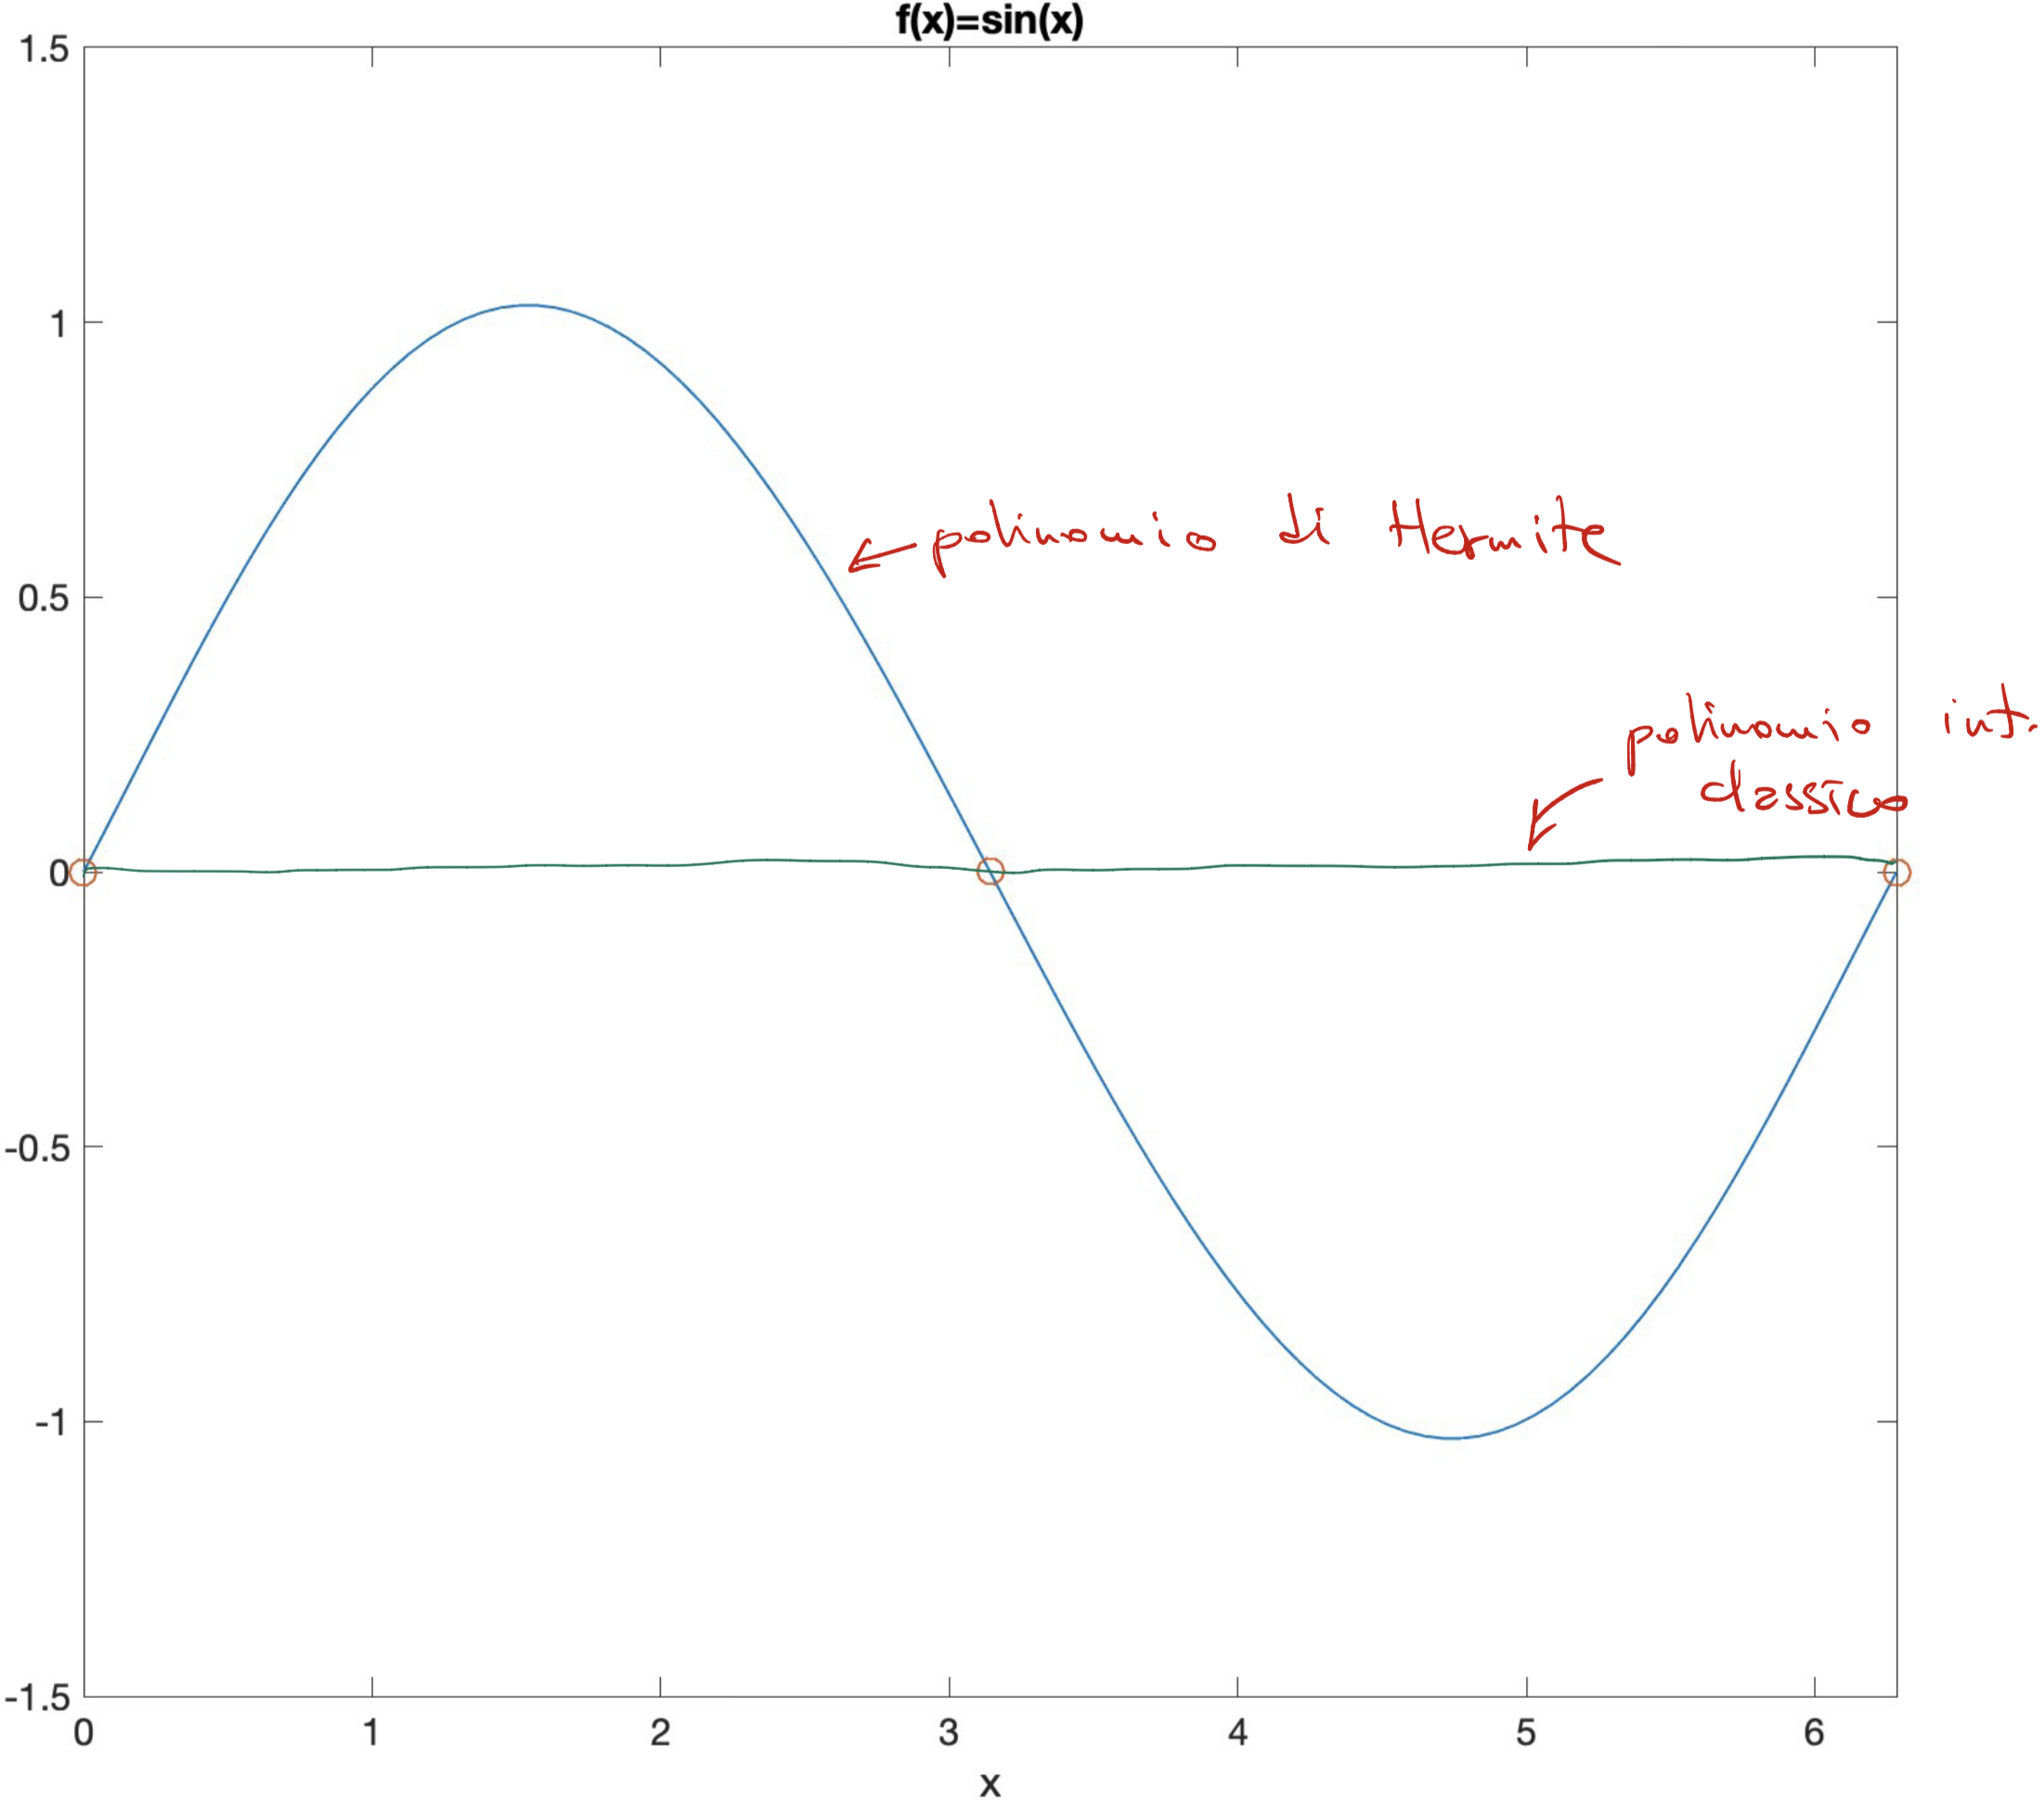
\includegraphics[width=0.5\textwidth]{immagini/PolHermite.png}
\caption{\label{fig:PolHermite} Esempio delle differenze di approssimazione}
\end{figure}
\begin{figure}
\centering
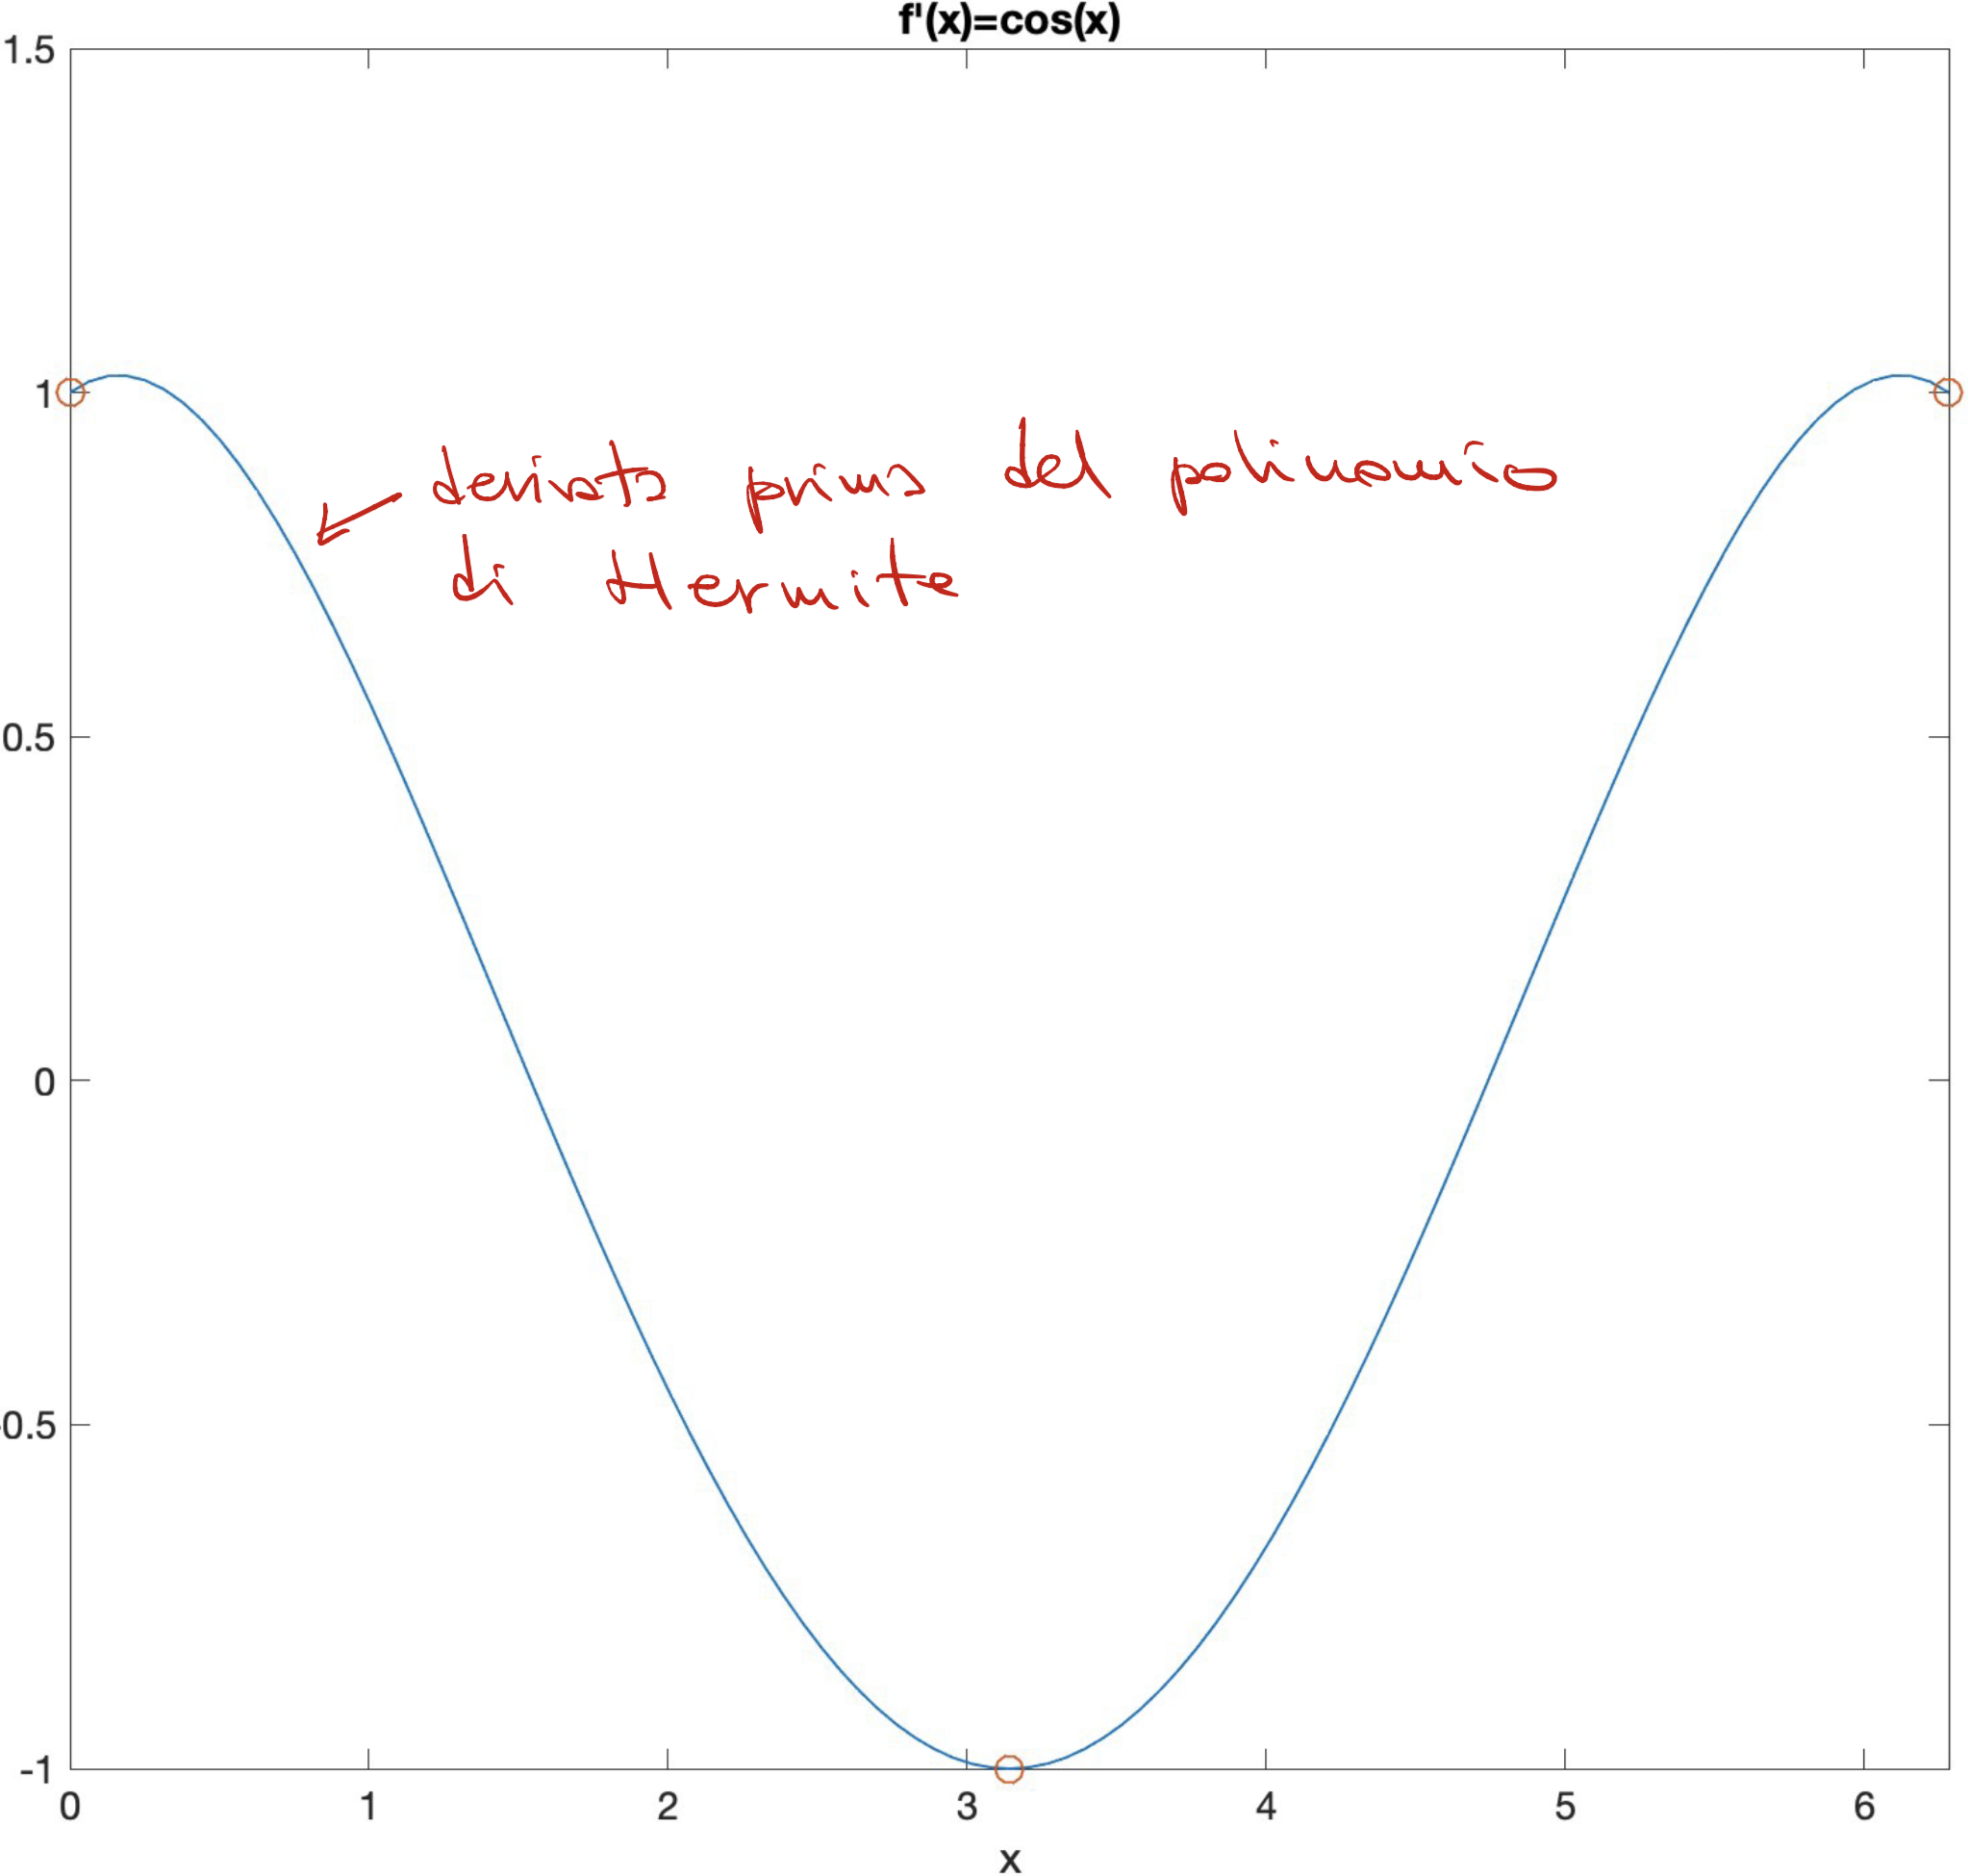
\includegraphics[width=0.5\textwidth]{immagini/PolHermite-1.png}
\caption{\label{fig:PolHermite1} Esempio delle differenze di approssimazione}
\end{figure}

\begin{remark}[Calcolo $p_H(x)$, caso semplice]
    Per il calcolo del polinomio di Hermite è utilizzata la sua forma di Newton: un caso semplice, per estrapolare una situazione generale, è con $n=2$, ovvero

    \begin{equation*}
        \begin{matrix}
            p_H(x)&=& f[x_0]\cdot 1\\
            &+& f[x_0,x_0](x-x_0)\\
            &+& f[x_0,x_0,x_1](x-x_0)^2\\
            &+& f[x_0,x_0,x_1,x_1](x-x_0)^2(x-x_1)\\
            &+& f[x_0,x_0,x_1,x_1,x_2](x-x_0)^2(x-x_1)^2\\
            &+& f[x_0,x_0,x_1,x_1,x_{\boldsymbol 2},x_{\boldsymbol 2}](x-x_0)^2(x-x_1)^2(x-x_{\boldsymbol 2}).
        \end{matrix}
    \end{equation*}
\end{remark}

Il risultato dell'osservazione è ottenuto immaginando di avere il doppio delle ascisse mediante l'utilizzo dell'indice $i+\frac{1}{2}$, dove le ascisse con questo indice tendono ad $x_i$ (analogo per le funzioni di base di Newton).
    
È importante osservare che da $f[x_0]$ è possibile arrivare a $f[x_0,x_0,x_1,x_1,x_2,x_2]$. Quest'ultima differenza divisa ha tutte le ascisse raddoppiate ed è possibile che l'ultimo polinomio di base di Newton abbia tutte le ascisse al quadrato, tranne l'$n$-esima (altrimenti avrebbe grado $2n+2$ invece di $2n+1$).

\begin{remark}[Calcolo $p_H(x)$, caso generale]
    In generale, per $\boldsymbol n$ generico, il polinomio di Hermite sarà ottenuto tramite 
    \begin{equation}\label{eq:polHerBaseNewt}
        p_H(x)=f[x_0]\cdot 1 + f[x_0,x_0]\cdot(x-x_0)+\hdots+f[x_0,x_0,\hdots,x_{\boldsymbol n},x_{\boldsymbol n}](x-x_0)^2\cdot\hdots\cdot(x-x_{\boldsymbol{n-1}})^2(x-x_{\boldsymbol n}).
    \end{equation}
    È possibile calcolare i coefficienti del polinomio, ovvero le differenze divise, con l'Algoritmo \ref{alg:calcDiffDivPolHer}, una variante dell'Algoritmo \ref{alg:calcDiffDiv}, tenendo di conto di (\ref{eq:equivApproxf'}). Nell'Algoritmo, il vettore in ingresso, \textbf{f} contiene i valori $f(x_0), f'(x_0), f(x_1), f'(x_1),\hdots, f(x_n),f'(x_n)$ ed in uscita, essendo sovrascritto, le differenze divise in (\ref{eq:polHerBaseNewt}).
\end{remark}
\begin{algorithm}
\caption{Polinomio di Hermite: calcolo delle differenze divise}\label{alg:calcDiffDivPolHer}
    \begin{lstlisting}[style=Matlab-editor]
    for i = (2*n+1):-2:3
        f(i) = (f(i)-f(i-2))/(x(i)-x(i-1))
    end
    for j = 2 : 2*n+1
        for i = (2*n+2) : -1 : j+1
            f(i) = (f(i)-f(i-1))/(x(i)-x(i-j))
        end
    end
    \end{lstlisting}
\end{algorithm}

Inoltre, è possibile calcolare $p_H(x)$ in Matlab tramite una versione modificata dell'algoritmo di Horner generalizzato (Algoritmo \ref{alg:polHornMod}), nella quale è utilizzato un vettore delle ascisse [\footnotemark] $x=[x_0\, x_0\, x_1\, x_1\, \hdots\, x_{n-1}\, x_{n-1}\,x_n]$, a patto di conoscere le differenze divise (ovvero i coefficienti del polinomio). 

\footnotetext{Le ascisse sono duplicate e per questo, nel ciclo implementato per il calcolo del polinomio, sarà contato fino ad $2n+1$. Il $+1$ è dovuto al fatto che $x_n$ è ripetuta solo una volta.}

È possibile capire come calcolare le differenze divise tramite il seguente esempio.
\begin{example}
    Considerando il caso in cui $\boldsymbol{n=1}$, il polinomio ha grado 3 seguendo la "formula" del calcolo del grado $(2n+1)$, e ritornando al caso in cui sono presenti le ascisse $x_{i+\frac{1}{2}}$ (quindi al caso in cui le ascisse sono duplicate):
    \begin{center}
        \begin{tabular}{|c|c|c|c|c|} 
        \hline
        & $\overset{\footnotemark}{0}$ & 1 & 2 & 3 \\
        \hline
        $x_0$ & $f[x_0]$ & & &\\
        $x_{\frac{1}{2}}$ & $f\left[x_\frac{1}{2}\right]$ & $f\left[\boldsymbol{x_0},\boldsymbol{x_\frac{1}{2}}\right]$ & &\\
        $x_1$ & $f[x_1]$ & $f\left[\boldsymbol{x_\frac{1}{2}},\boldsymbol{x_1}\right]$ & $f[\boldsymbol{x_0},x_{\frac{1}{2}}, \boldsymbol{x_1}]$ &\\
        $x_{\frac{3}{2}}$ & $f\left[x_\frac{3}{2}\right]$ & $f\left[\boldsymbol{x_1},\boldsymbol{x_\frac{3}{2}}\right]$ & $f\left[\boldsymbol{x_\frac{1}{2}},x_1,\boldsymbol{x_\frac{3}{2}}\right]$ & $f\left[\boldsymbol{x_0}, x_\frac{1}{2}, x_1, \boldsymbol{x_\frac{3}{2}}\right]$\\
        \hline
        \end{tabular}
    \end{center}\footnotetext{Differenza tra l'indice delle ascisse utilizzando la proprieta' incrementale delle differenze divise.}
    Le ascisse in \textbf{grassetto} sono quelle la cui differenza va a denominatore nel calcolo della rispettiva differenza divisa. 
    
    Operando il \textbf{limite} per $\boldsymbol{x_{i+\frac{1}{2}}\rightarrow x_i}$:
    \begin{center}
        \begin{tabular}{|c|c|c|c|c|} 
        \hline
        & 0 & \textbf{1} & 2 & 3 \\
        \hline
        $x_0$ & $f[x_0]$ & & &\\
        $x_0$ & $f[x_0]$ & \fbox{$f[\boldsymbol{x_0},\boldsymbol{x_0}]$} & &\\
        $x_1$ & $f[x_1]$ & $f[\boldsymbol{x_0},\boldsymbol{x_1}]$ & $f[\boldsymbol{x_0},x_0, \boldsymbol{x_1}]$ &\\
        $x_1$ & $f[x_1]$ & \fbox{$f[\boldsymbol{x_1},\boldsymbol{x_1}]$} & ${f[\boldsymbol{x_0}},x_1,\boldsymbol{x_1}]$ & $f[\boldsymbol{x_0}, x_0, x_1, \boldsymbol{x_1}]$\\
        \hline
        \end{tabular}
    \end{center}
    
    Le differenze divise cerchiate sono le differenze divise per le quali non è noto il metodo di calcolo. 
    
    Per un generico $\boldsymbol n$ non è possibile calcolare direttamente le differenze divise in colonna $\boldsymbol{1}$ \fbox{$f[x_i,x_i],\; i=0,\hdots,n,$} tuttavia è possibile quanto segue:
    \begin{equation*}
        \boldsymbol{f[x_i,x_i]}=\lim_{x_{i+\frac{1}{2}}\to x_i}\frac{f\left(x_{i+\frac{1}{2}}\right)-f(x_i)}{x_{i+\frac{1}{2}}+x_i}=\boldsymbol{f'(x_i)}.
    \end{equation*}
\end{example}

Pertanto, è possibile modificare leggermente l'algoritmo classico per il calcolo delle differenze divise (ovvero l'Algoritmo \ref{alg:calcDiffDiv}), in modo che, dove sono presenti ascisse ripetute, sia utilizzato il corrispondente valore della derivata della funzione $f(x)$, come appena esposto. In questo modo sono presenti tutti gli elementi per implementare efficientemente il calcolo del polinomio interpolante di Hermite nella sua forma di Newton.

\begin{remark}
    Nella tabella precedente, utilizzata per il calcolo delle differenze divise, il vettore delle ascisse uilizzato è del tipo $x=[x_0\, x_0\, x_1\, x_1 \hdots x_{\boldsymbol n}\, x_{\boldsymbol n}].$
\end{remark}

\subsection{Errore nell'interpolazione polinomiale}\label{ssec:errInter}\footnote{Slide 2-23 PDF 19, PG 86-87.}
È necessario studiare il comportamento della funzione errore $e$ definita come
\begin{equation}\label{eq:defErrInter}
    \boldsymbol{e(x)=f(x)-p(x)},\quad x\in [a,b],
\end{equation}
per la quale è possibile osservare che $f(x)=p(x)+e(x)$, con $e(x)$ errore commesso nell'approssimazione di $f(x)$ tramite il polinomio interpolante $p(x)$.

\begin{figure}
    \centering
    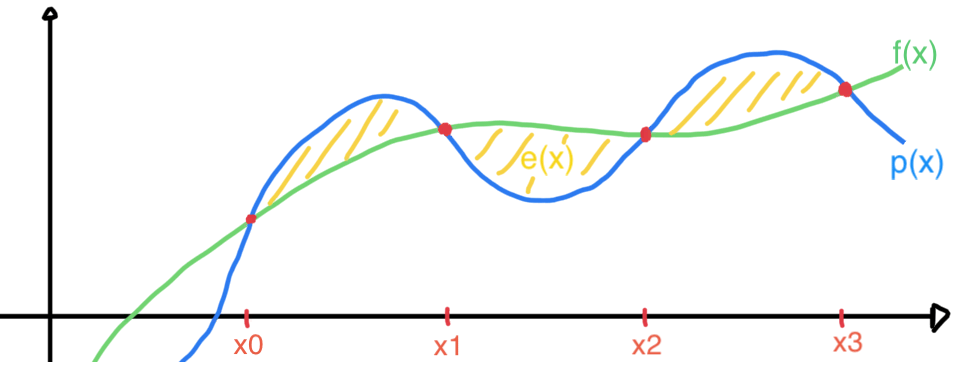
\includegraphics[width=0.5\textwidth]{immagini/ErrorePolinomioHermite.png}
    \caption{Esempio dell'errore $e$ del polinomio Hermite $p$ rispetto a $f$.}
    \label{fig:errPolHer}
\end{figure}
 
\begin{remark}
    \footnote{Slide 3, PDF 19. Da (\ref{eq:condInterp}) segue l'osservazione.} $e(x_i)=f(x_i)-p(x_i)=f(x_i)-f(x_i)=0,\; i=0,\hdots,n.$
\end{remark}

Pertanto, è noto che nelle ascisse di interpolazione l'errore si annulla. È necessario stabilire quanto $e(x)$ sia "distante" da 0, per $x\notin \{x_0,\hdots, x_n\}.$

\begin{theorem}\label{th:errInterFormaNewt}
    \footnote{Slide 3 PDF 19, TH 4.3 PG 86.} Dato $p(x)$, polinomio interpolante $f(x)$, definito come (\ref{eq:polInterNewt}), sulle ascisse distinte (definite come in (\ref{eq:ascisseDistinte})), vale:
    \begin{equation}\label{eq:errInterFormaNewt}
        \boldsymbol{e(x)=f[x_0,x_1,\hdots,x_n,x]\,\omega_{n+1}(x),\quad w_{n+1}(x)=\prod_{j=0}^{n}(x-x_j)}.
    \end{equation}
\end{theorem}

\begin{proof}
    \footnote{Sfrutta il fatto che è possibile costruire il polinomio interpolante nella forma di Newton in modo incrementale.} Fissato $\widehat x\notin\overbrace{\{x_0,\hdots,x_n\}}^{\text{ascisse d'interp.}}$ un punto generico, il polinomio $\widehat p(x)\in\Pi_{n+1}$ è costruito come segue:
    \begin{equation*}
        \begin{matrix}
            \widehat p(x_i)&=&f(x_i),& i=0,\hdots,n,\\
        \widehat p(\widehat x) &=& f(\widehat x),
        \end{matrix}
    \end{equation*}
    Ovvero, $\widehat p(x)$ interpola $f(x)$ anche in $\widehat x$, oltre che nelle ascisse $x_0,\hdots,x_n$.
    
    (È imposta la seguente condizione:) Utilizzando la forma di Newton del polinomio interpolante (Teorema \ref{th:formaNewt}) è ottenuto che
    \begin{equation*}
        \underset{\footnotemark}{\widehat p(x)} = p(x) + f[x_0,\hdots,x_n,\widehat x]\,\omega_{n+1}(x),
    \end{equation*}
    la quale soddisfa le condizioni di interpolazione
    \begin{equation*}
        \widehat p(x_i)=\equalto{p(x_i)}{f(x_i)} + f[x_0,\hdots,x_n,\widehat x]\,\overbrace{\omega_{n+1}(x_i)}^{0} \boldsymbol = f(x_i),\quad i=0,\hdots,n,
    \end{equation*}
    ed inoltre:
    \begin{equation*}
        \widehat p(\widehat x)=p(\widehat x)+ f[x_0,\hdots,x_n,\widehat x]\,\omega_{n+1}(\widehat x)\boldsymbol = f(\widehat x).
    \end{equation*}
    Da quest'ultima uguaglianza è ottenuto che
    \begin{equation*}
        \boldsymbol{e(\widehat x)\equiv} \underbrace{f(\widehat x) - p(\widehat x)}_{\text{errore di $\widehat x$}}=f[x_0,\hdots,x_n,\widehat x]\,\omega_{n+1}(\widehat x).
    \end{equation*}
    L'aaserto discende dal fatto che $\widehat x$ è un punto generico. [\footnotemark]
\end{proof}

\addtocounter{footnote}{-1}
\footnotetext{Quando è calcolato in una delle ascisse $x_i$, si annulla sia il polinomio di interpolazione che la funzione. Il coefficiente $f[x_0,\hdots,x_n,\widehat x]$ permette di ottenere le seguenti condizioni di accuratezza (ovvero le condizioni di interpolazione che seguono).}

\stepcounter{footnote}
\footnotetext{Se al posto di $\widehat x$ è sostituito $x$ allora $\widehat p(x)$ continua a variare.}

\begin{remark}
    Il Teorema \ref{th:errInterFormaNewt} definisce la forma dell'errore di interpolazione polinomiale (e di conseguenza è necessario impararlo).
\end{remark}

\begin{corollary}
    \footnote{Slide 5 PDF 19, Corollario 4.1 PG 87; Importante perché esiste un legame tra le differenze divise e le derivate della funzione $f$, se questa è sufficientemente regolare.}
    Utilizzando le ipotesi del Teorema \ref{th:errInterFormaNewt} e supposto che $f\in C^{(n+1)}$ sul più piccolo intervallo contenente le ascisse in argomento alla differenza divisa in (\ref{eq:errInterFormaNewt}), allora (vedere (\ref{eq:P4DiffDiv})):
    \begin{equation}\label{eq:errInterP4}
        \begin{matrix}
            e(x)=\frac{f^{(n+1)}(\xi_x)}{(n+1)!}\,\omega_{n+1}(x),&\\
            &\xi_x\in[\min\{\underset{i}{\min}\,x_i,\,x\},\, \max\{\underset{i}{\max}\,x_i,\, x\}]\boldsymbol{\equiv I(x)}.
        \end{matrix}
    \end{equation}
\end{corollary}

\begin{remark}[Errore polinomio di Hermite]\label{rem:errPolHerm}
    \footnote{Da sapere. Slide 5 PDF 19, Oss. 4.4 PG 87.}
    Per il polinomio di Hermite (\ref{eq:polHerBaseNewt}) interpolante la funzione $f(x)\left(\in C^{(2n+2)}[I(x)]\right)$, sulle ascisse $x_0,\hdots,x_n$, l'errore corrispondente al polinomio è definito come
    \begin{equation}\label{eq:errPolInterHer}
        e_H(x)= f(x)-p_H(x) \overset{\footnotemark}{=} f[\overbrace{x_0,x_0,\hdots,x_n,x_n,x}^{2n+3}]\,\omega^2_{n+1}(x)\equiv\frac{\boxed{f^{(2n+2)}(\widehat\xi_x)}}{(2n+2)!}\,\omega^2_{n+1}(x).
    \end{equation}
\end{remark}
$e_H(x)$ è di grado $2n+2$.
\footnotetext{Le funzioni di base del polinomio di Newton hanno ascisse raddoppiate.}

\begin{remark}\footnote{Slide 5 PDF 19.}
    Da quanto esposto nell'Osservazione \ref{rem:errPolHerm} è ottenuta una controprova del fatto che:
    \begin{enumerate}
        \item $p(x)\equiv f(x),\; \text{se } f(x)\in\Pi_n\; \left(f^{(n+1)}\equiv 0\right)$;
        \item $p_H(x)\equiv f(x),\; \text{se } f(x)\in\Pi_{2n+1}\; \left(f^{(2n+2)}\equiv 0\right)$.
    \end{enumerate}
\end{remark}

\begin{remark}\label{rem:consErrInterP4}\footnote{Slide 6 PDF 19.}
    Osservando la struttura dell'errore (\ref{eq:errInterP4})
    \begin{center}
        $e(x)=\,\boxed{\boxed{\frac{f^{(n+1)}(\xi_x)}{(n+1)!}}\;\boxed{\omega_{n+1}(x)}}$
    \end{center}
\end{remark}
(analoghe considerazioni varranno per $e_H(x)$), è possibile osservare che questo è costituito da due parti:
\begin{itemize}
    \item la prima che dipende da $\boxed{f(x)}$, per cui, più $f(x)$ è regolare, tanto più velocemente questo termine tende a 0, per $n\rightarrow\infty$ (dovuto a $(n+1)!$ al denominatore);
    \item la seconda, $\boxed{\omega_{n+1}(x)=\prod_{j=0}^n(x-x_j)}$, dipende solo dalla scelta delle ascisse di interpolazione.
    
    È necessario osservare che, per $x>\underset{i}{\max}\{x_i\}$ o per $x<\underset{i}{\min}\{x_i\},\, \omega_{n+1}(x)\approx x^{n+1}$ (vedere Figura \ref{fig:ossErrInterp}). Da questa considerazione è evinto che $x$ debba essere scelta nel più piccolo intervallo che contiene le ascisse di interpolazione (in Figura \ref{fig:ossErrInterp} tra $x_0$ e $x_2$). \textbf{Quindi sarà scelta $\boldsymbol{x\in [a,b]}$ che contiene le ascisse}.
\end{itemize}

\begin{figure}
    \centering
    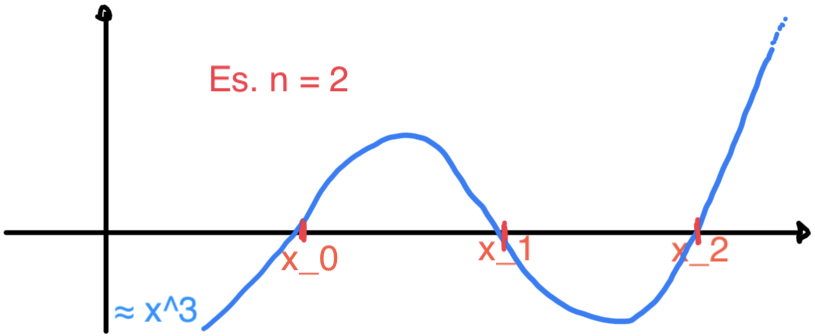
\includegraphics[width=0.5\textwidth]{immagini/es. n=2.png}
    \caption{\label{fig:ossErrInterp} Esempio con numero di ascisse $n=2$.}
\end{figure}

Il polinomio interpolante coincide con la funzione $f$, come per il riquadro principale di $e(x)$ nell'Osservazione \ref{rem:consErrInterP4}, se $f$ è un polinomio di grado al più $n$ con la sua derivata $(n+1)$-esima che si annulla identicamente. Quindi, se la funzione $f$ è un polinomio di grado al più $n$ l'errore è identicamente nullo, il che significa che il polinomio interpolante coincide con la funzione di Hermite (ovvero l'uguaglianza (\ref{eq:errPolInterHer})).

Data l'interpolazione di Hermite su $n+1$ ascisse (il polinomio interpolante di Hermite è di grado $2n+1$), se la funzione interpolante è un polinomio di grado al più $2n+1$, ancora una volta, il polinomio di Hermite coinciderà con la funzione interpolante. Ciò viene confermato dalla parte riquadrata in (\ref{eq:errPolInterHer}), in quanto la derivata $(2n+1)$-esima di un polinomio di grado $2n+1$ è identicamente nulla.

Con funzioni "buone" è possibile aspettarsi che $p(x)$ approssimi sempre meglio $f(x)$, per $n\rightarrow\infty$.

Come misura dell'errore, negli esempi che seguono, è considerata la norma infinito:
\begin{equation*}
    ||e||\overset{\footnotemark}{=} \overbrace{\underset{\boldsymbol{a\leq x\leq b}}{\max}|\underbrace{f(x)-p(x)}_{e(x)}|}^{\footnotemark}\approx \underset{\boldsymbol{x=a+i\frac{b-a}{N},\, i=0,\hdots,N}}{\max}|e(x_i)|,\quad N>>1\; (N=\boldsymbol{10000}).
\end{equation*}
\addtocounter{footnote}{-1}
\footnotetext{Norma uniforme, ovvero continua nell'intervallo $[a,b]$.}
\stepcounter{footnote}
\footnotetext{Che è una norma in $C^{(0)}[a,b]$.}

$||e||$ sarà approssimata, dato che non è possibile calcolarla, con la differenza in valore assoluto, calcolato su un numero molto ampio di ascisse. $||e||$ è una sottostima ed è buona se è utilizzato un numero accettabile di punti ($N>10000$).

\paragraph{Progetto e scelta di $N$:} Per il progetto $N$ deve essere molto grande. Negli esempi richiesti nell'elaborato non saranno ammessi $N<10000$ (saranno considerati sbagliati). Inoltre, per un polinomio di grado 5 assegnare $N=3$ sarà considerato sbagliato in quanto la sottostima dell'errore è importante.

\begin{example}
    Per $f(x)=\sin(x)$ è possibile ottenere ottimi risultati (vedere Figure \ref{fig:approxErrIntepolaz4}-\ref{fig:approxErrIntepolaz19}), utilizzando un numero di ascisse crescenti ed equidistanti, dato che tutte le derivate di $\sin(x)$ sono limitate.

    Date le Figure \ref{fig:approxErrIntepolaz4}-\ref{fig:approxErrIntepolaz19}, per $f(x)=\sin(x)$, è ottenuto un numero crescente di ascisse equidistanti, dato che le derivate di $\sin(x)$ sono tutte limitate.
\end{example}

\begin{figure}%[H]
\centering
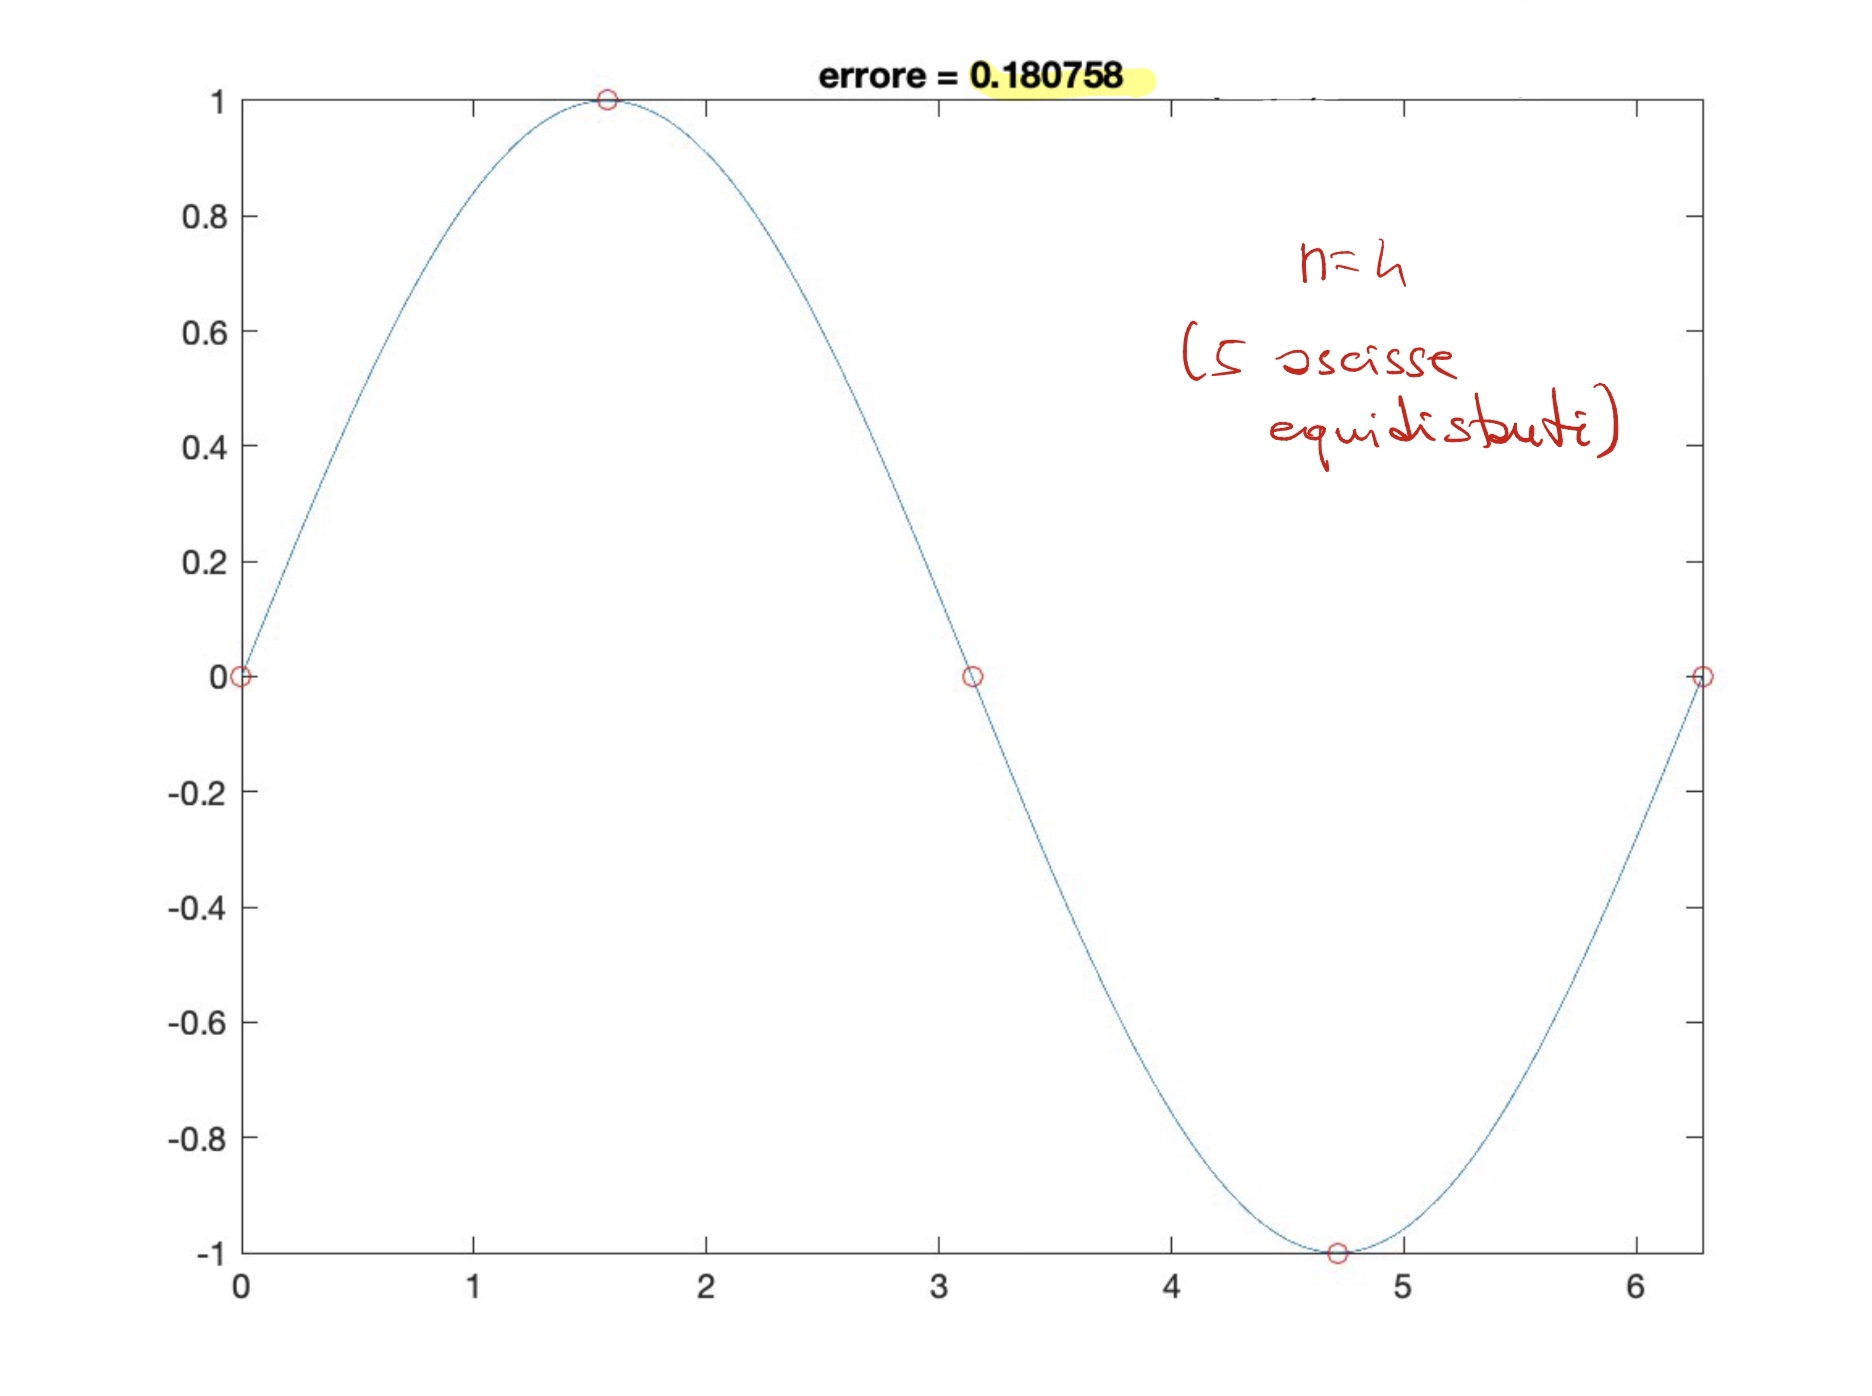
\includegraphics[width=0.55\textwidth]{immagini/sin(n=4).jpg}
\caption{Esempio con numero di ascisse $n=4$.}\label{fig:approxErrIntepolaz4}
\end{figure}

\begin{figure}%[H]
\centering
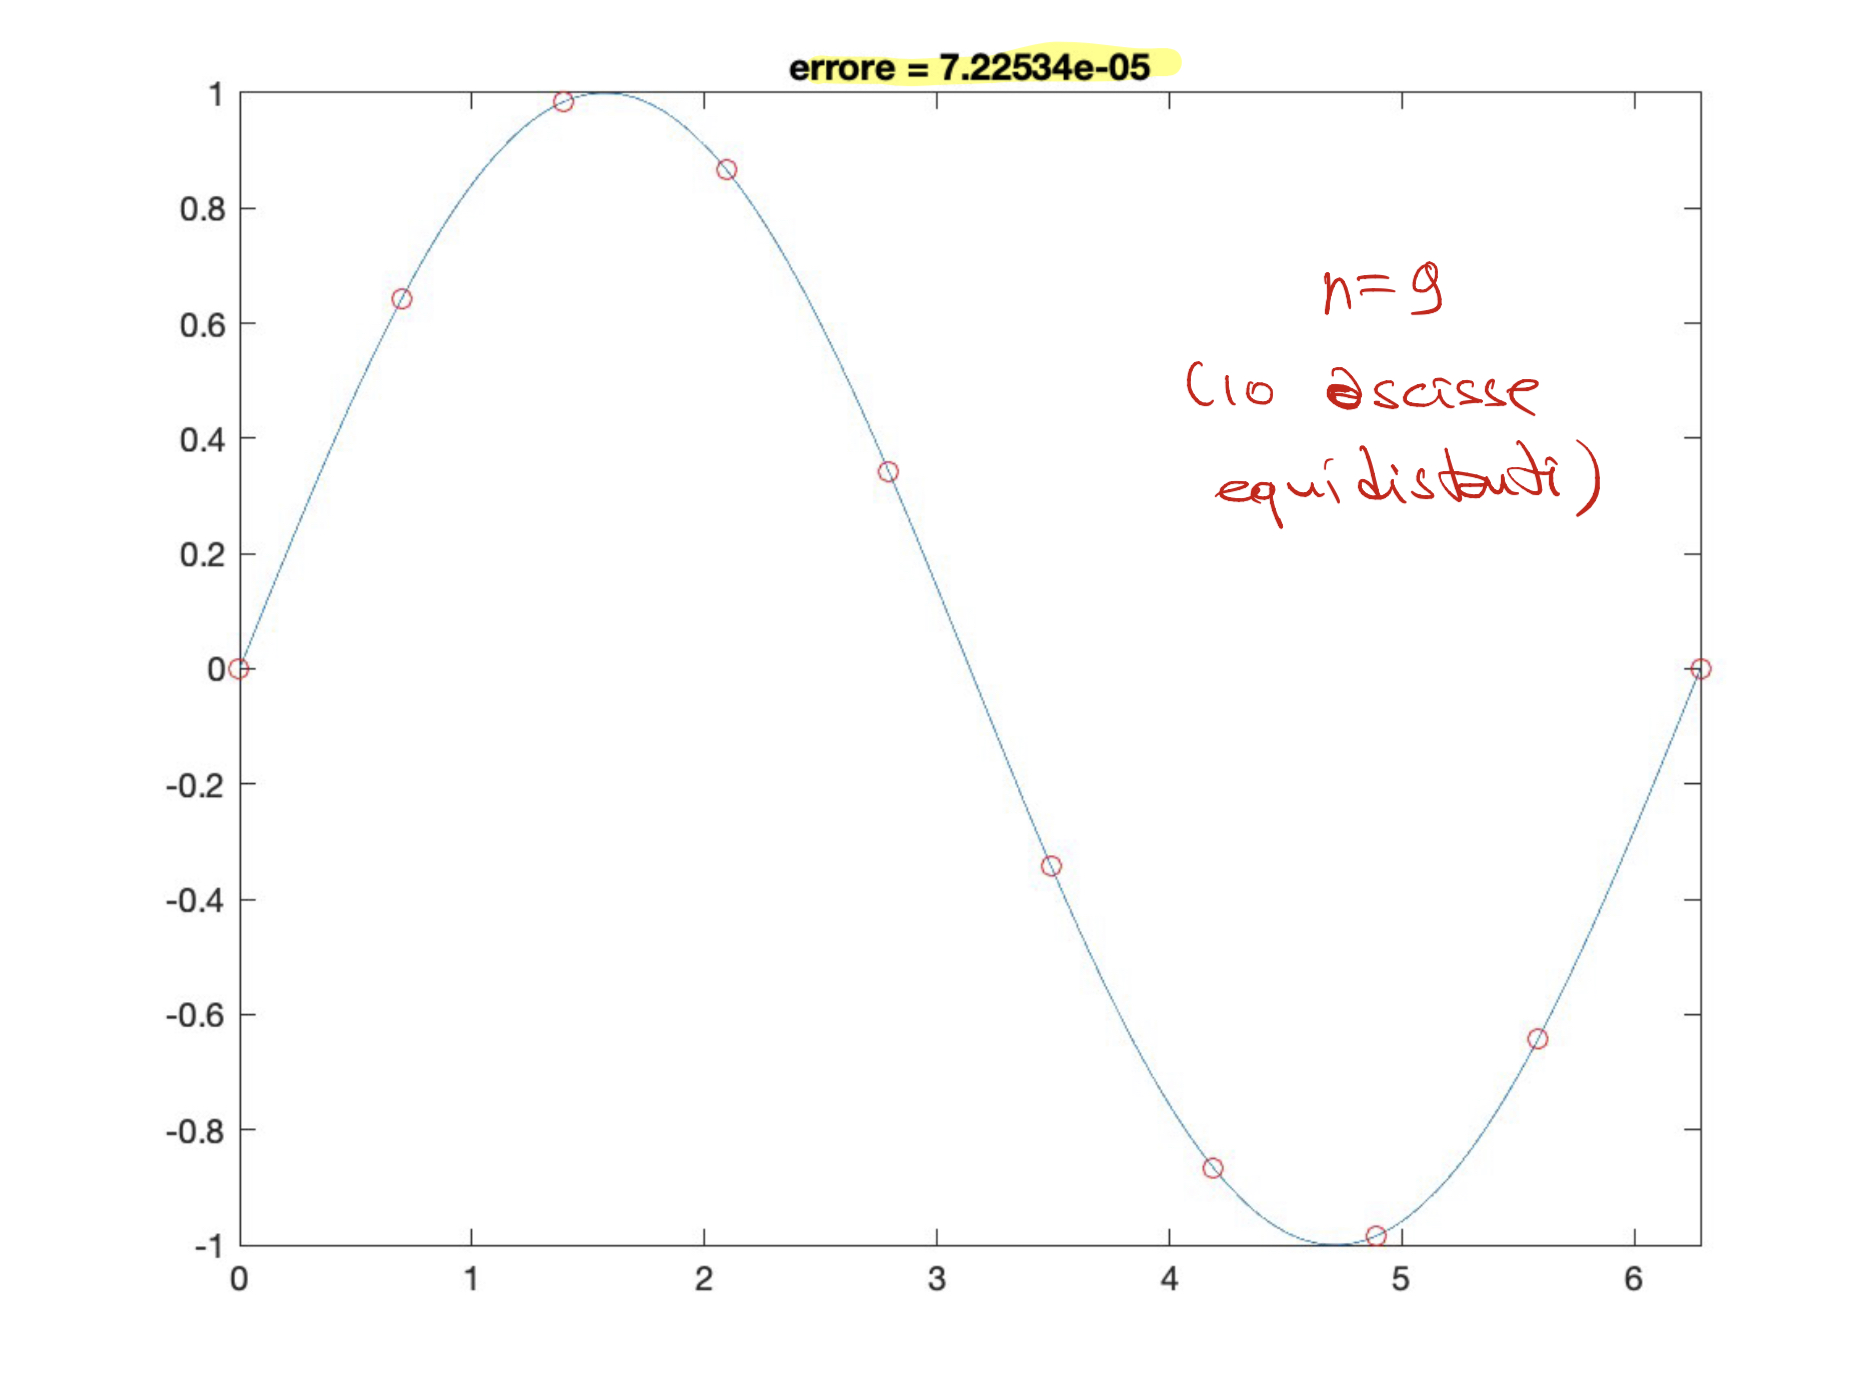
\includegraphics[width=0.5\textwidth]{immagini/sin(n=9).jpg}
\caption{Esempio con numero di ascisse $n=9$.}\label{fig:approxErrIntepolaz9}
\end{figure}

\begin{figure}%[H]
\centering
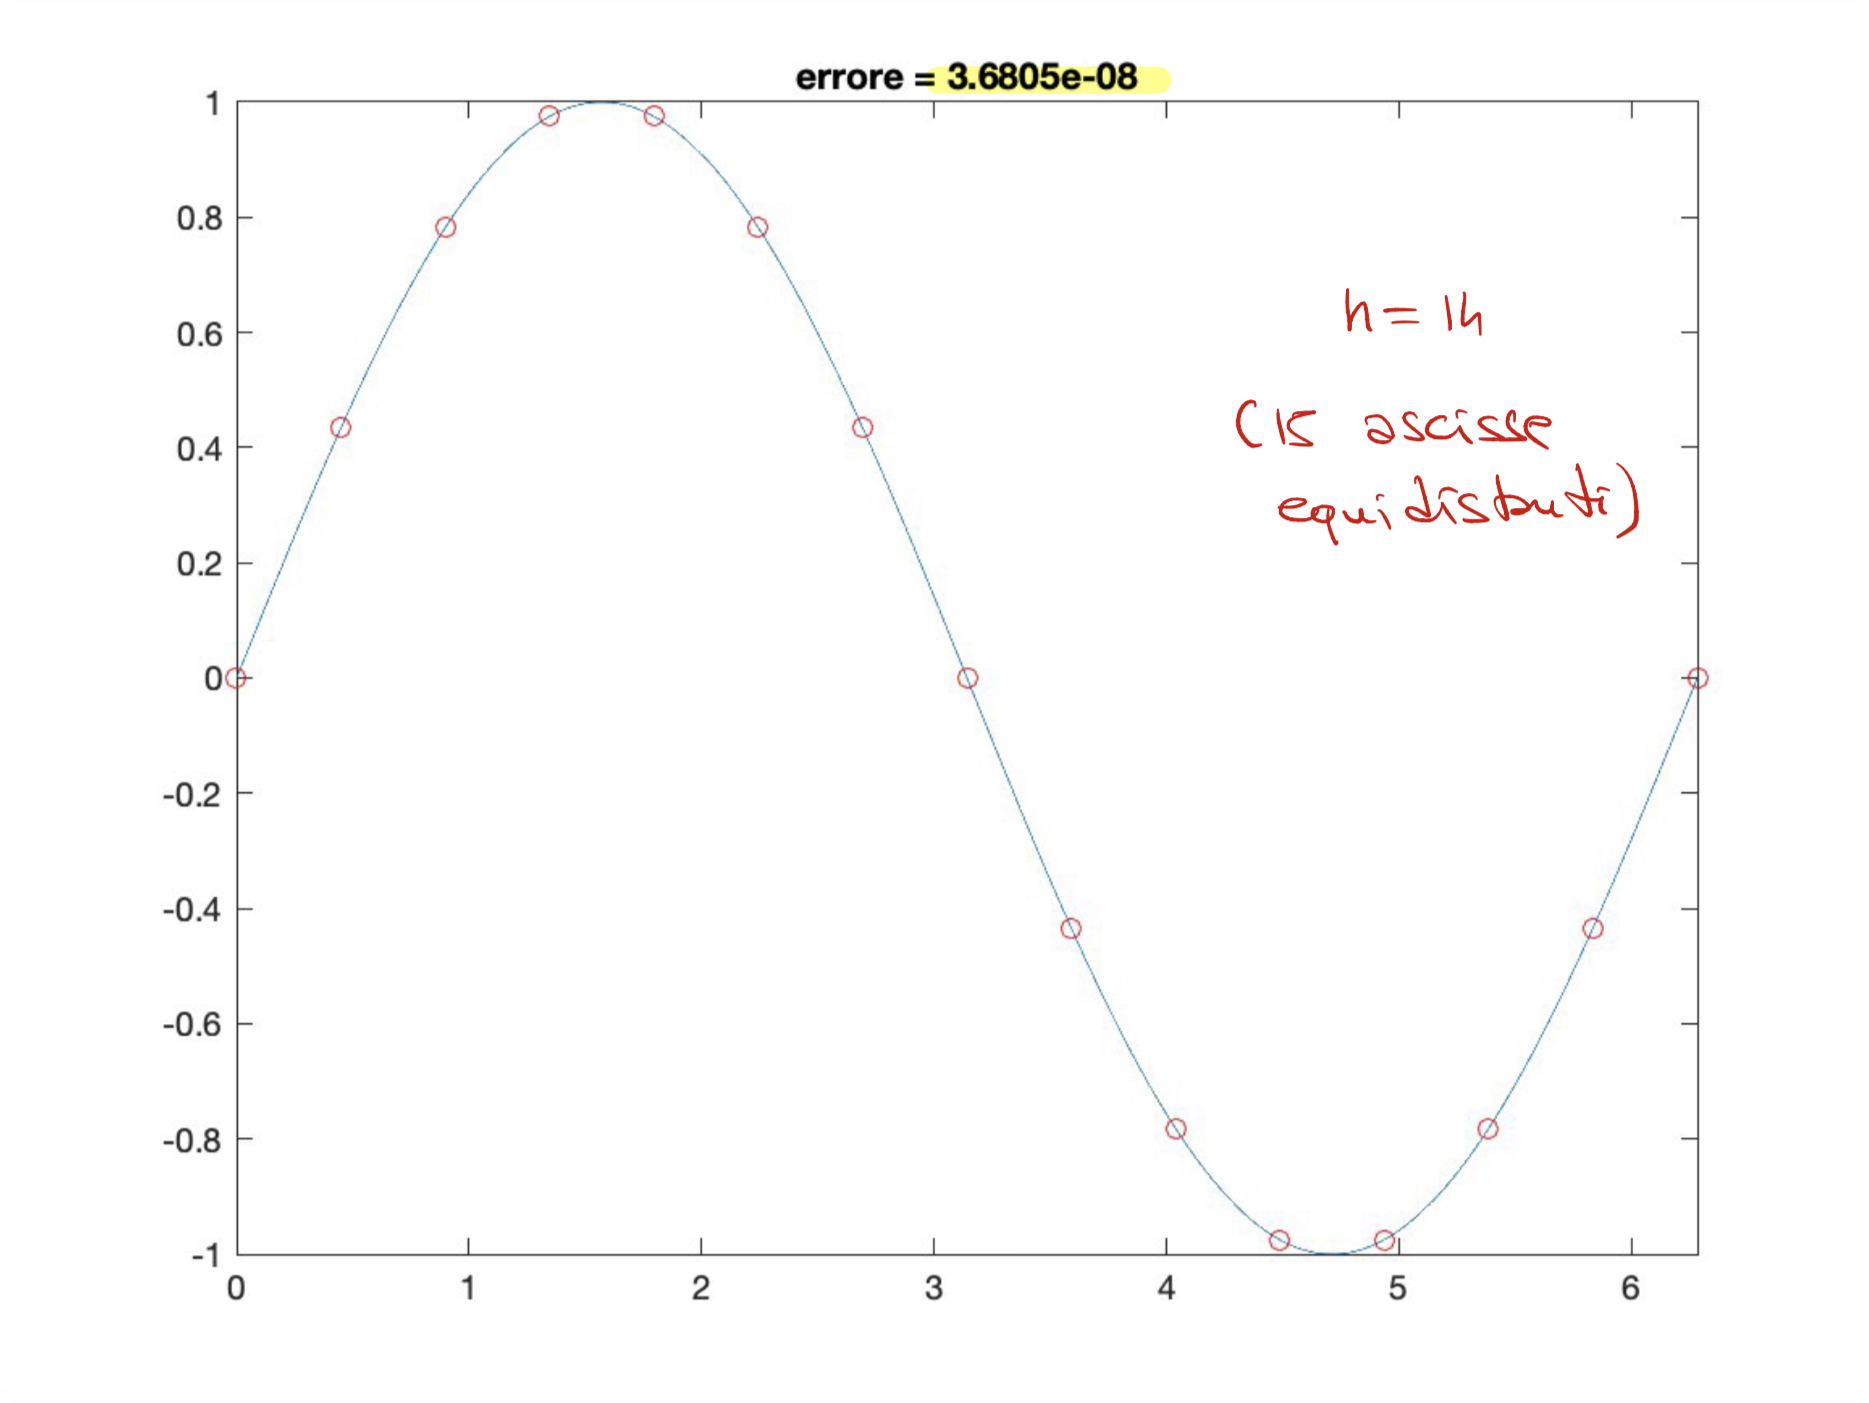
\includegraphics[width=0.5\textwidth]{immagini/sin(n=14).jpg}
\caption{Esempio con numero di ascisse $n=14$.}\label{fig:approxErrIntepolaz14}
\end{figure}

\begin{figure}%[H]
\centering
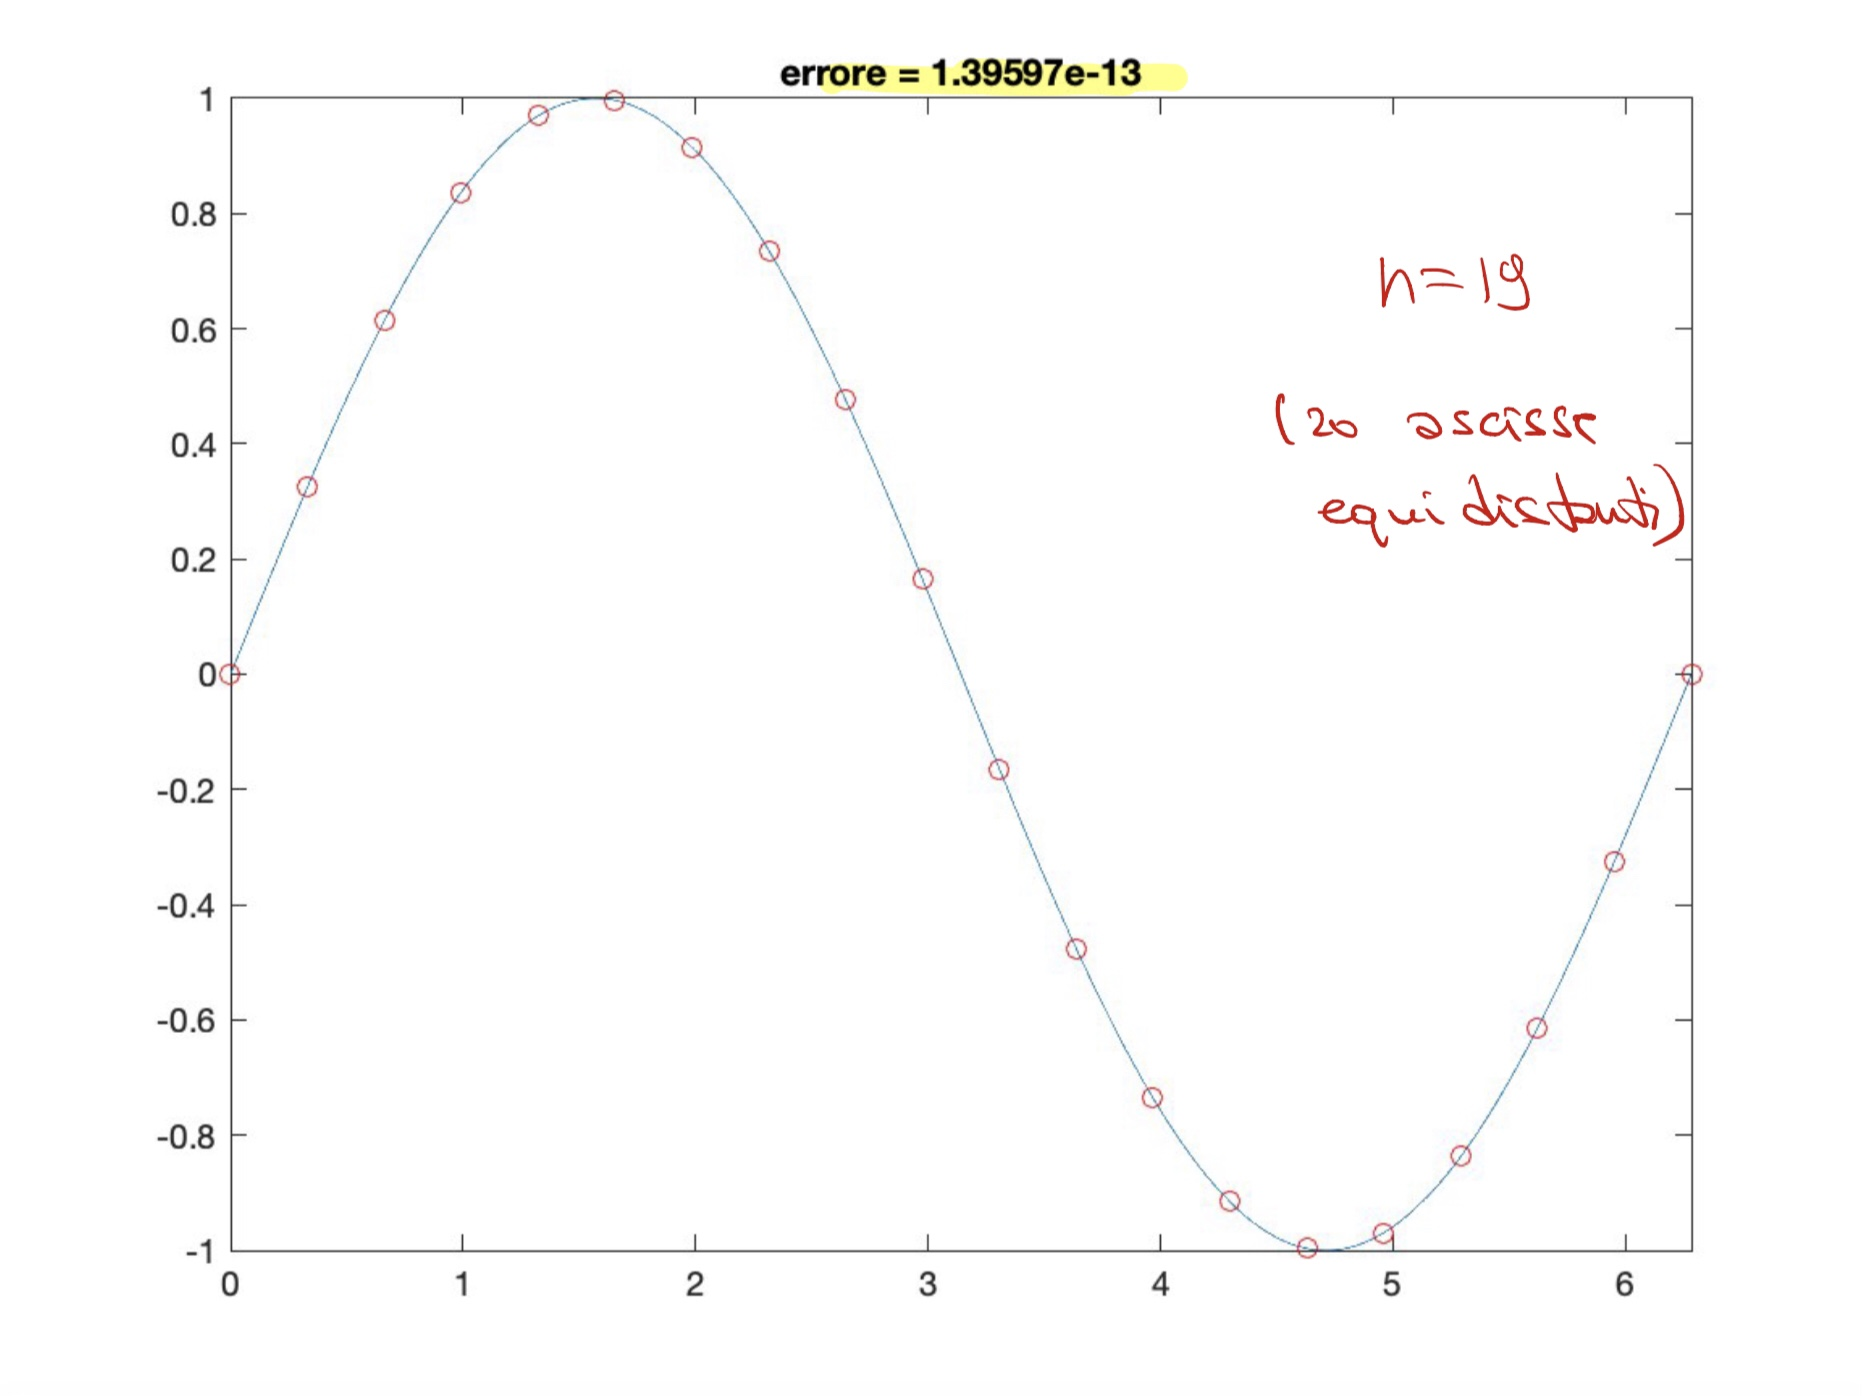
\includegraphics[width=0.5\textwidth]{immagini/sin(n=19).jpg}
\caption{Esempio con numero di ascisse $n=19$.}\label{fig:approxErrIntepolaz19}
\end{figure}

È possibile provare, come nel precedente esempio, appplicare un numero di ascisse crescenti ed equidistanti, applicando la formula di Runge, alla seguente funzione (grafico  Figura \ref{fig:funzRunge-5,5}):
\begin{equation}\label{eq:funzExRunge}
    f(x)\overset{\footnotemark}{=}\frac{1}{1+x^2},\quad x\in [-5,5].
\end{equation}

\footnotetext{Simmetrica rispetto all'asse $y$ e massimo in $x=0$, vedere Figura \ref{fig:funzRunge-5,5}.}

\begin{figure}
    \centering
    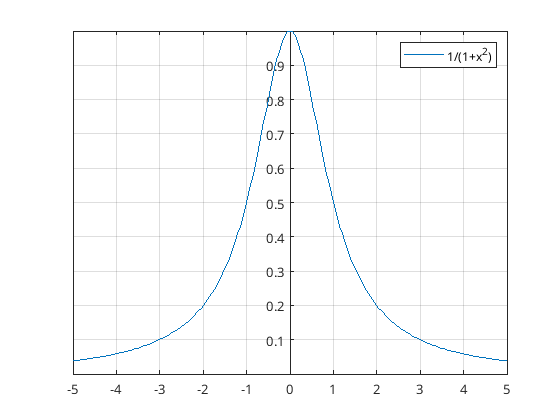
\includegraphics[width=0.5\textwidth]{immagini/funzioneRunge-5,5.png}
    \caption{Grafico di (\ref{eq:funzExRunge})}\label{fig:funzRunge-5,5}
\end{figure}

Nelle Figure \ref{fig:funzRunge_n=2}-\ref{fig:funzRunge_n=22} [\footnote{Nelle figure i puntini rappresentano la funzione di Runge.}] è utilizzata la funzione di Runge per approssimare (\ref{eq:funzExRunge}), con un numero crescente di ascisse equidistanti.

\begin{figure}
    \centering
    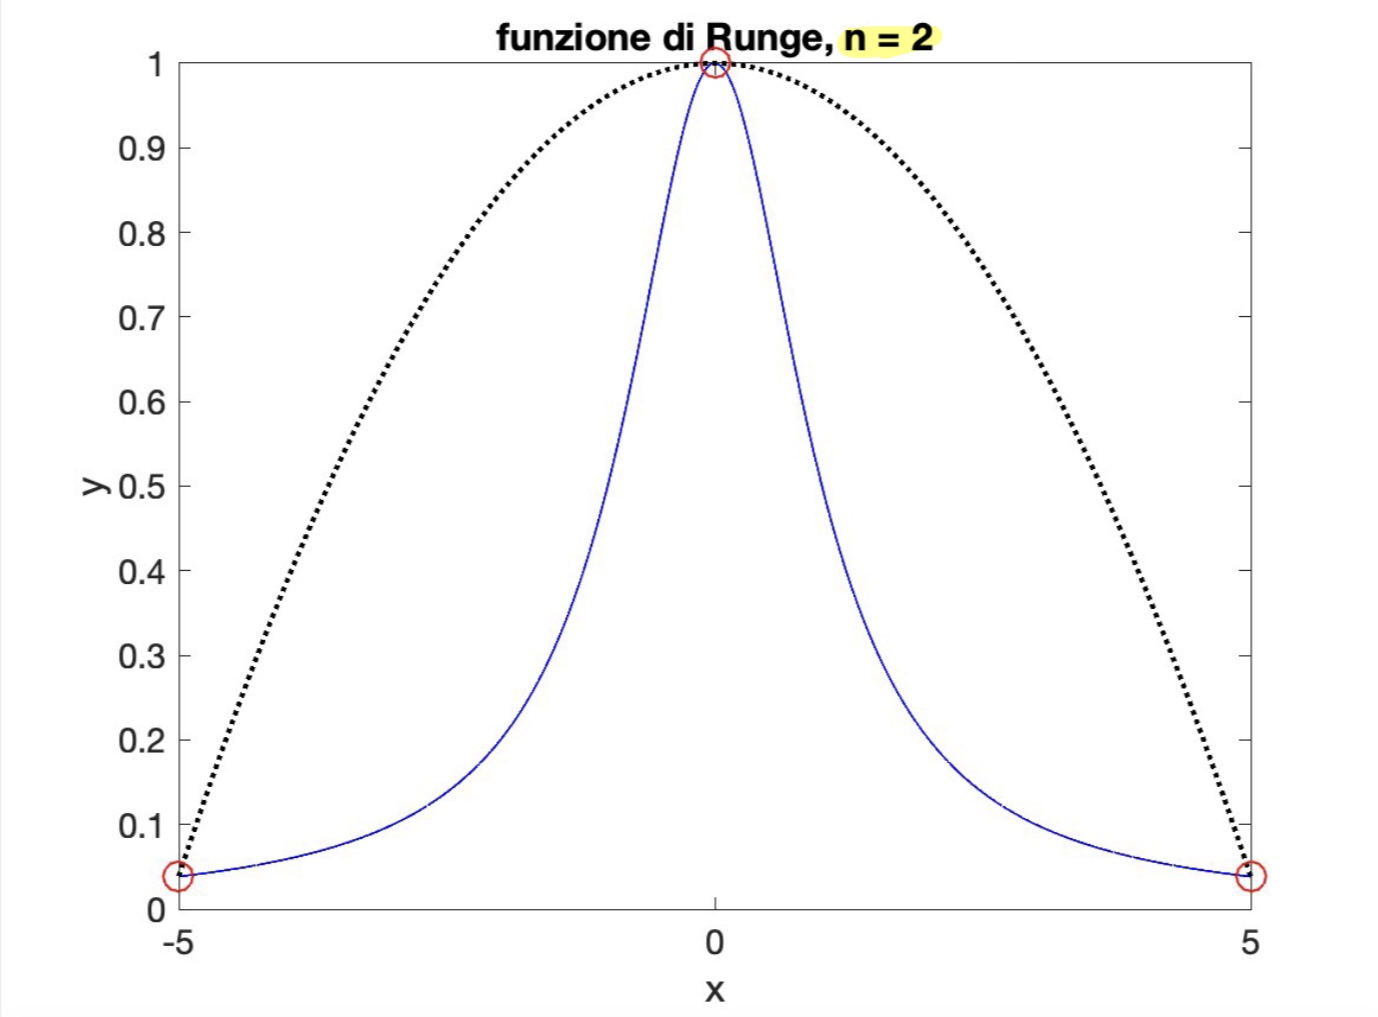
\includegraphics[width=0.5\textwidth]{immagini/funzioneRunge_n=2.jpg}
    \caption{Approssimazione di (\ref{eq:funzExRunge})}\label{fig:funzRunge_n=2}
\end{figure}
\begin{figure}
    \centering
    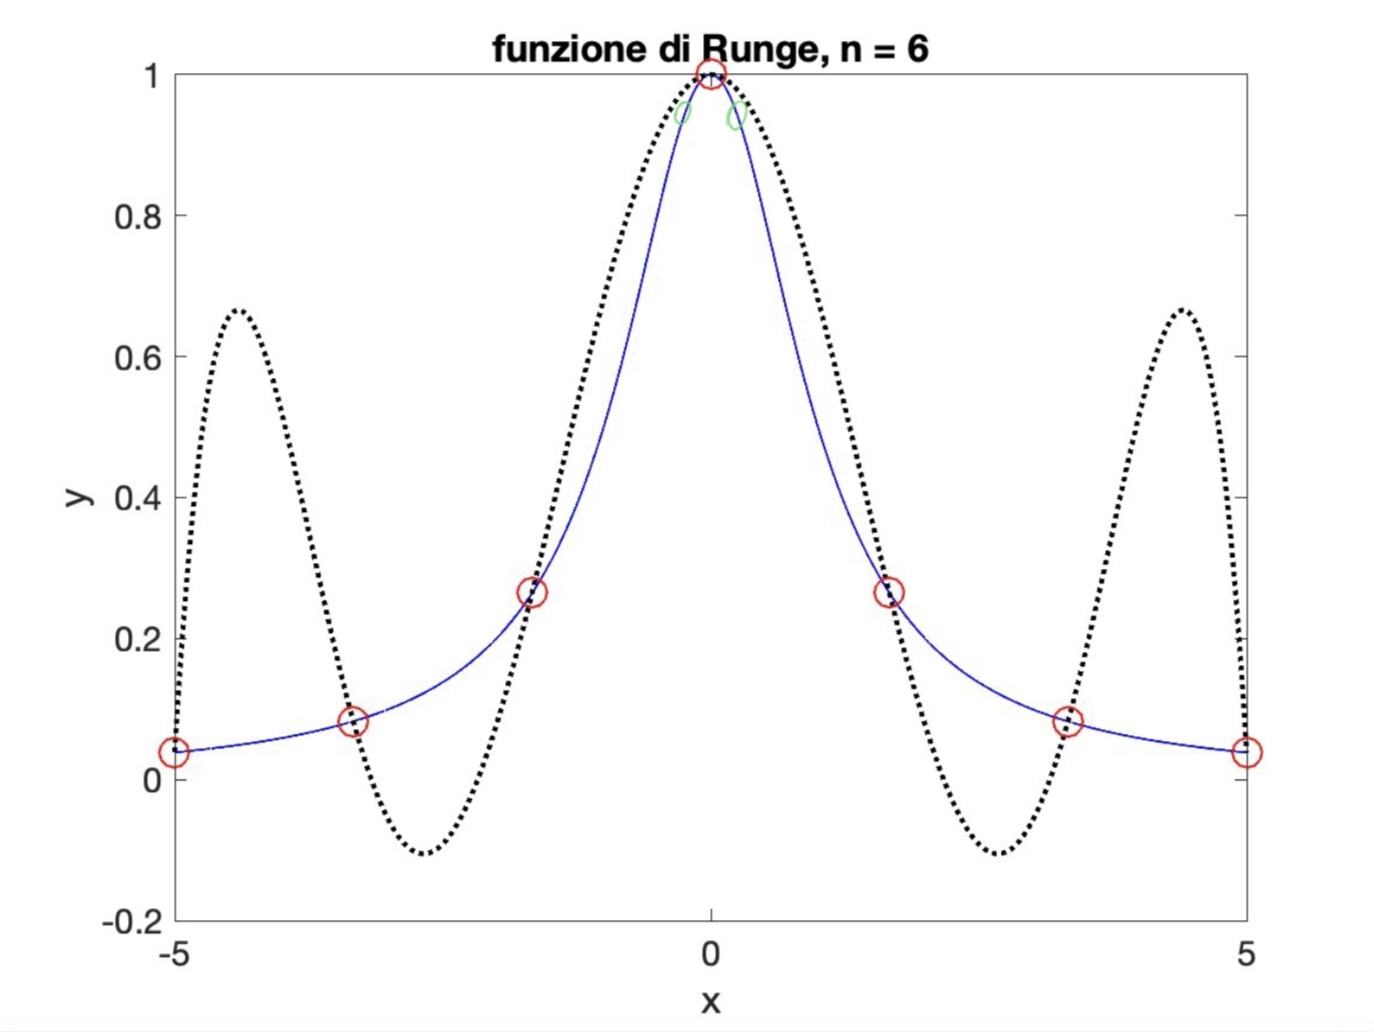
\includegraphics[width=0.5\textwidth]{immagini/funzioneRunge_n=6.jpg}
    \caption{Approssimazione di (\ref{eq:funzExRunge})}\label{fig:funzRunge_n=6}
\end{figure}
\begin{figure}
    \centering
    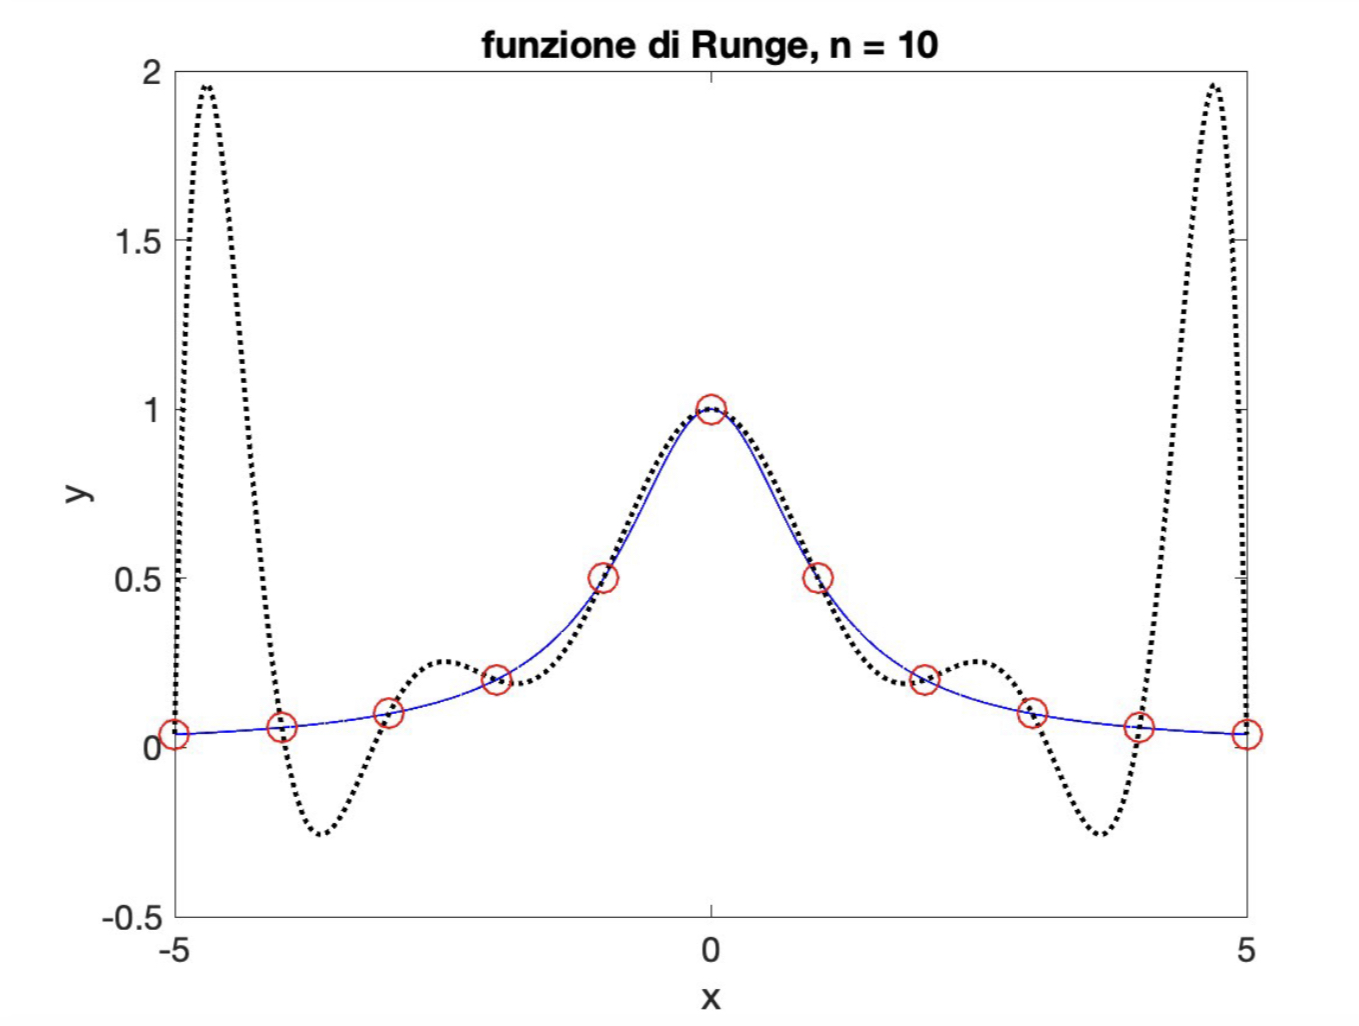
\includegraphics[width=0.5\textwidth]{immagini/funzioneRunge_n=10.jpg}
    \caption{Approssimazione di (\ref{eq:funzExRunge})}\label{fig:funzRunge_n=10}
\end{figure}
\begin{figure}
    \centering
    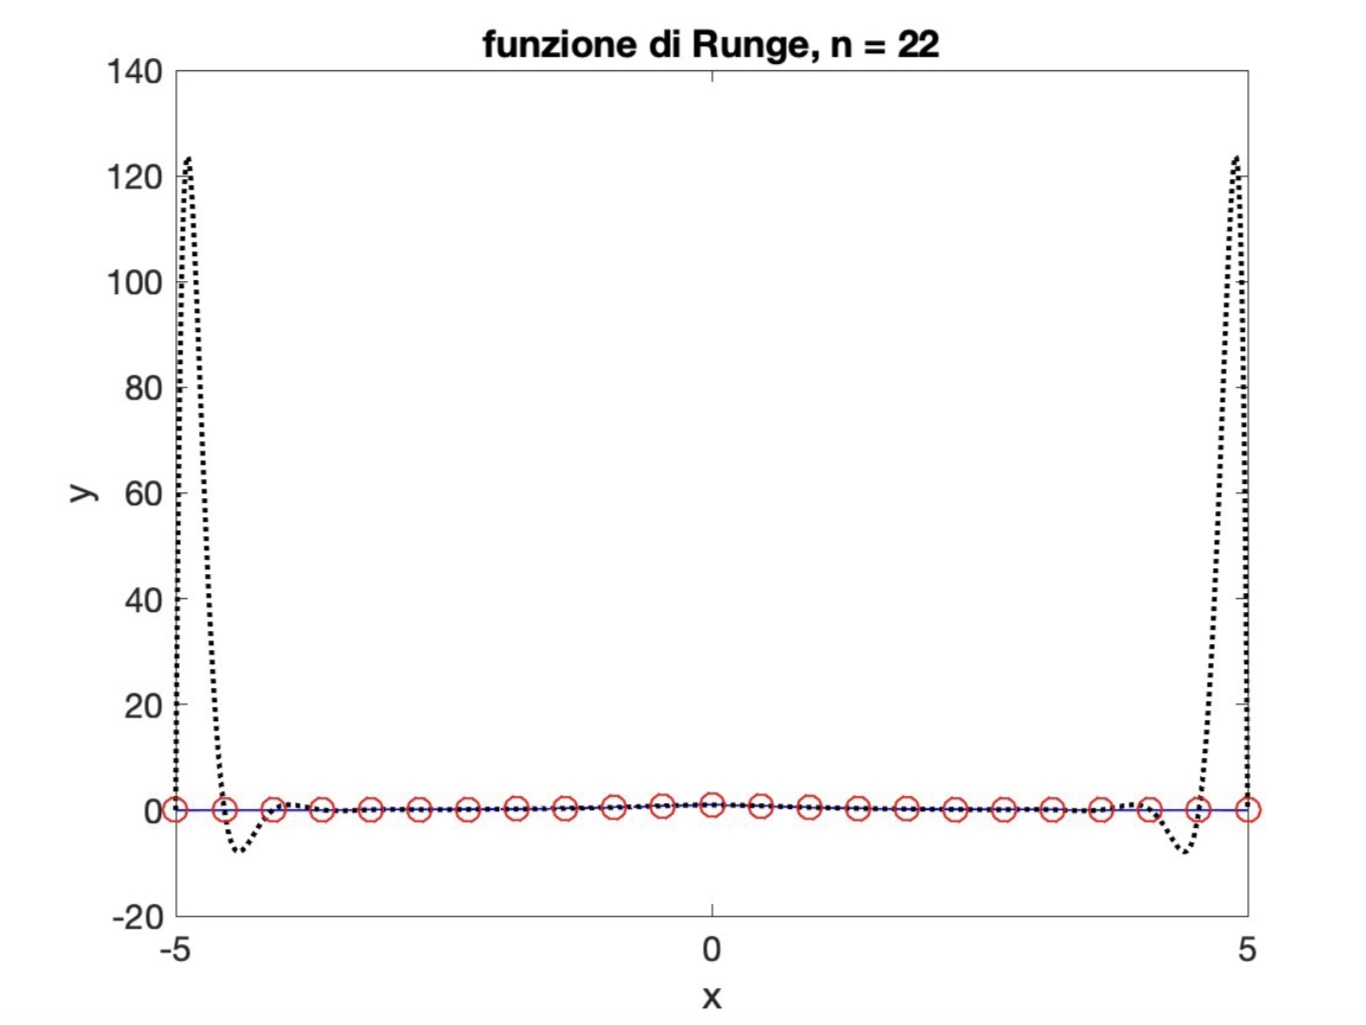
\includegraphics[width=0.5\textwidth]{immagini/funzioneRunge_n=22.jpg}
    \caption{Approssimazione di (\ref{eq:funzExRunge})}\label{fig:funzRunge_n=22}
\end{figure}

\begin{remark}[Dettagli impotanti per il progetto]
    Distinguere fra numeri pari e dispari di ascisse è importante. Se $n$ è pari allora  le ascisse sono dispari. Un esempio è graficare il polinomio (\ref{eq:funzExRunge}) per un valore pari di $n$, quindi con un numero dispari di ascisse (ovvero $n+1$), così da trovare i punti cerchiati in rosso delle Figure \ref{fig:funzRunge_n=2}-\ref{fig:funzRunge_n=22} con un metodo affidabile.  Avere un numero di ascisse dispari permette di trovare il massimo della funzione in modo più efficace rispetto ad avere un numero pari di ascisse (vedere Figura \ref{fig:funzRunge_n=6}). Inoltre, nel caso del numero di ascisse pari, l'errore diventa importante (una parte di funzione viene tagliata fuori).
\end{remark}

In genere è possibile verificare che $e(x)\rightarrow\infty,\;\, n\rightarrow\infty$, quindi il problema è malcodizionato. Tuttavia, è necessario studiare il condizionamento del problema dell'interpolazione dove, per ciascuna delle classi di problemi considerati, è noto quale sia il coefficiente di perturbazione del problema.

È necessario studiare il problema del condizionamento dell'interpolazione polinomiale, ovvero: date le ascisse di interpolazione (\ref{eq:ascisseDistinte}), è definito il polinomio $p(x)\in\Pi_n$ interpolante la funzione $f(x)\in\Pi_n$ come
\begin{equation*}
 \boldsymbol{p(x_i)=f(x_i)},\quad\boldsymbol{i=0,\hdots,n}.
\end{equation*}

Considerando una funzione $\Tilde{f}(x)$, perturbazione di $f(x)$, e costruito $\tilde{p}(x)$, il polinomio interpolante $\Tilde{f}(x)$ sulle ascisse (\ref{eq:ascisseDistinte}), come
\begin{equation*}
 \boldsymbol{\tilde{p}(x_i)=\tilde{f}(x_i),\quad i=0,\hdots,n},
\end{equation*}
allora sono introdotte le seguenti misure degli errori:

\begin{itemize}
    \item $||f-\Tilde{f}||$, misura degli errori sui dati di ingresso;
    \item $||p-\Tilde{p}||$, misura degli errori sul risultato (minore è migliore è il condizionamento del problema).
\end{itemize}

Il problema riguarda anche come sono scelte le ascisse di interpolazione.

\subsection{Condizionamento del problema}\label{ssec:condProbApproxfun}
Il problema del condizionamento dell'errore prima citato può essere "trasformato" nello studio di come $||p-\Tilde{p}||$ dipenda da $||f-\Tilde{f}||$. Studiare il condizionamento del problema significa stabilire in che modo piccole perturbazioni del problema, ovvero $||f-\Tilde{f}||$, si riflettano con perturbazioni sul risultato, ovvero su $||p-\Tilde{p}||$:
\begin{itemize}
    \item se le perturbazioni sul risultato sono piccole allora il problema è ben condizionato;
    \item se piccole perturbazioni ne provacano di grandi sul risultato il problema è malcondizionato.
\end{itemize}

Ciò che sarà studiato è il problema della valutazione del polinomio interpolante.

%%\vspace{6px}
%%\hrule
%%\vspace{-7px}
\paragraph{Intermezzo}{Lo studio del condizionamento è svolto in aritmetica esatta. Non è svolto in aritmetica finita in quanto sarebbe necessario studiare le singole operazioni elementari e verificare come gli errori si propagano per ognuna di essa. Lo studio del condizionamento è uno studio semplificato della modalità con la quale gli errori si propagano.

Quindi, lo studio deò condizionamento di un problema sarà fatto in aritmetica esatta. Questo significa che qualunque rappresentazione algebrica del polinomio interpolante è equivalente. Ciò non è vero in aritmetica finita, il metodo di calcolo del polinomio influisce sul risultato finale, quindi due metodi di calcolo diversi non forniranno il medesimo risultato.}
%%\vspace{5px}
%%\hrule
%%\vspace{6px}

Al fine di avere una misura degli errori è necessario introdurre la norma infinito su $C^{(0)}[a,b]:$

\begin{equation}\label{eq:defNormaInfG}
    \forall g\in C^{(0)}[a,b]\,:\, ||g||\overset{\footnotemark}{=}\underset{a\leq x\leq b}{\max}|g(x)|.
\end{equation}\footnotetext{Applicazione del Teorema di Weistrass: esiste un massimo per $g$ perché questa è limitata tra $a$ e $b$.}

Da quanto appena scritto, per $x\in [a,b]$, è ottenuto che
\begin{equation*}
    \begin{matrix}
        \left|p(x)-\Tilde{p}(x)\right|&\overset{\footnotemark}{=}&
        \left|\sum_{i=0}^nf_i\,L_{in}(x)-\sum_{i=0}^n\Tilde{f}_i\, L_{in}(x)\right|&\overset{\footnotemark}{=}&\left|\sum_{i=0}^n(f_i-\Tilde{f}_i)\,L_{in}(x)\right|\\
        &\overset{\footnotemark}{\leq}&
        \sum_{i=0}^n|f_i-\Tilde{f}_i|\,|L_{in}(x)|&\leq&\underbrace{\left(\sum_{i=0}^n|L_{in}(x)|\right)}_{\footnotemark}\underbrace{\underset{i=0,\hdots,n}{\max}|f_i-\Tilde{f}_i|}_{\lambda_n(x)}\\
        &\leq&\boldsymbol{\boldsymbol{\lambda_n(x)}}\cdot\,||f-\Tilde{f}||,
    \end{matrix}
\end{equation*}

\addtocounter{footnote}{-3}
\footnotetext{Utilizzata la forma di Lagrange perché il contributo della funzione è evidenziato rispetto ad un numero generico delle ascisse, i polinomi di base di Lagrange ne usufruiscono.}

\stepcounter{footnote}
\footnotetext{Raccoglimento di $L_{in}(x)$.}

\stepcounter{footnote}
\footnotetext{Applicazione della diseguaglianza triangolare: il modulo di una somma è minore uguale della somma dei loro moduli.}

\stepcounter{footnote}
\footnotetext{Massimo dei valori assoluti della differenza $f_i-\Tilde{f},\; i=0,\hdots,n$ (ovvero la norma $||f - \Tilde{f}||$), anche se $x_1,\hdots,x_n\in [a,b]$. La differenza  $f_i-\Tilde{f}$ è minore della norma $||f_i-\Tilde{f}||$ che segue nella diseguaglianza. \\
Inoltre è possibile affermare quanto segue:$\underset{i=0,\hdots,n}{\max}|f_i-\Tilde{f}_i|=\underset{i=0,\hdots,n}{\max}|f(x_i)-\Tilde{f}(x_i)|\leq\underset{a\leq x\leq b}{\max}|f(x)-\Tilde{f}(x)|=||f-\Tilde{f}||$.}

\noindent dove $\boldsymbol{\lambda_n(x)}$ è la \textbf{funzione di Lebesque}. Tale funzione è positiva per definizione e dipende solo dalla scelta delle ascisse di interpolazione. Pertanto, dalla precedente disuguaglianza è ottenuto che
\begin{equation*}
    \forall x\in [a,b]:\; |p(x)-\Tilde{p}(x)|\leq\lambda_n(x)||p-\Tilde{p}||\Rightarrow  ||p-\Tilde{p}||\leq ||\lambda_n\cdot\underbrace{||f-\Tilde{f}||}_{\footnotemark}||=\underbrace{||\lambda_n||}_{\boldsymbol{\Lambda_n}}\cdot||f-\Tilde{f}||,
\end{equation*}
\footnotetext{Costante positiva da portare fuori.}

\noindent dove $\boldsymbol{\Lambda_n=||\lambda_n||}$ è detta \textbf{costante di Lebesque}. Questa costante misura la massima amplificazione sul risultato dell'errore sui dati di ingresso e definisce il numero di condizionamento. Per questo è ottenuto quanto segue:
\begin{equation}\label{eq:maggPertDiffPTildeP}
    \boxed{\underbrace{||\equaltoup{p}{f(x)}-\equaltoup{\Tilde{p}}{\Tilde{f}(x)}||}_{\footnotemark}\leq\boldsymbol{\Lambda_n}\,\underbrace{||f-\Tilde{f}||}_{\footnotemark}}
\end{equation}

\addtocounter{footnote}{-1}
\footnotetext{Misura dell'errore sul risultato.}

\stepcounter{footnote}
\footnotetext{Misura degli errori in ingresso.}

Data l'importanza della costante di Lebesque è utile sturdiarne alcune importanti proprietà.

\noindent$\boldsymbol{\Lambda_n}$ \textbf{è indipendente dal particolare intervallo $[a,b]$ considerato.} Questa proprietà è importante perché se i risultati sono contenuti in un uno specifico intervallo di riferimento, allora le ascisse di interpolazione dell'intervallo speficico sono estendibili ad uno generico intervallo che le contiene.

Date $a\leq\underbrace{x_0<\hdots<x_n}_{\footnotemark}\leq b$, allora
\begin{equation}\label{eq:xi}
    \xi=\frac{x-a}{b-a}, 
\end{equation}
dove $\xi$ è una trasformazione lineare, per $x=a\Rightarrow\xi = 0$ e per $x=b\Rightarrow\xi = 1$. Pertanto, se $x\in [a,b] \Rightarrow\xi\in [0,1]$; viceversa, se $\xi\in [0,1]\Rightarrow \boldsymbol{x=a+(b-a)\,\xi},\, x\in [a,b]$.

\footnotetext{Saranno trasformate linearmente sull'intervallo $[0,1]$.}

Alle ascisse di interpolazione $x_i\in [a,b]$ corrispondono
\begin{equation}\label{eq:xii}
    \xi_i=\frac{x_i-a}{b-a}\in [0,1],\quad \forall i=0,\hdots,n.
\end{equation}

È possibile provare che i polinomi di base di Lagrange, definiti sulle ascisse $\{x_i\}$, coincidano con quelli costruiti sulle ascisse $\{\xi_i\}$, attraverso le prossime uguaglianze:

\begin{equation*}
    \begin{matrix}
        \boldsymbol{L_{in}(x)} &=&\prod_{j=0, j\neq i}^n\frac{\overset{\footnotemark}{x}-x_j}{x_i-x_j}&&&&&&\\
        \boldsymbol{L_{in}(\xi)} &=& \prod_{j=0,j\neq i}^n\frac{\xi-\xi_j}{\xi_i-\xi_j}&\overset{\footnotemark}{=}&\prod_{j=0, j\neq i}^n\frac{\frac{x-a}{b-a}-\frac{x_j-a}{b-a}}{\frac{x_i-a}{b-a}-\frac{x_j-a}{b-a}}&\overset{\footnotemark}{=}&\\
        &&\prod_{j=0,j\neq i}^n\frac{x-a-(x_j-a)}{x_i-a-(x_j-a)}&=&\prod_{j=0,j\neq i}^n\frac{x-x_j}{x_i-x_j}&=&\boldsymbol{L_{in}(x)}.\\
        &&&&&&&&\qed
    \end{matrix}
\end{equation*}

\addtocounter{footnote}{-2}
\footnotetext{Sarà trasformato in $x=a+(b-a)\,\xi$, ovvero $\xi=\frac{x-a}{b-a}$.}

\stepcounter{footnote}
\footnotetext{Per $(\ref{eq:xi})\overset{\text{e}}{+}(\ref{eq:xii})$.}

\stepcounter{footnote}
\footnotetext{Evidenziato $(b-a)$ e semplificato.}

L'intervallo di riferimento non è importante, in quanto è possibile definire le seguenti proprietà, le quali valgono considerando solo il numero delle ascisse, ovvero:

\begin{itemize}
    \item [P1)] ridefinendo la norma sull'intervallo $[0,1]$, la costante di Lebesque rimane invariata. Questo è dovuto dal fatto che, se i polinomi coincidono, allora anche la costante di Lebesque, ottenuta come somma dei due polinomi, non dipende dall'intervallo $[a,b]$. L'unica differenza è nella definizione di norma perché definita per $x\in[a,b]$;
    \item [P2)] qualunque sia la scelta delle ascisse (distinte tra loro), è noto che $\Lambda_n\geq O(\log n)$;
    \item[P3)] dalla precedente proprietà deriva che $\Lambda_n\rightarrow\infty,\; n\rightarrow\infty$, quindi il problema diviene malcondizionato al crescere di $n$;
    \item[P4)] la scelta di ascisse equidistanti da una costante di Lebesque genera una successione $\{\Lambda_n\}$, la quale diverge esponenzialmente con $n\rightarrow\infty$. Pertanto, la scelta di ascisse equidistanti non è, in generale, appropriata.
\end{itemize}

\subsubsection{Connesssioni tra condizionamento ed errore dell'interpolazione polinomiale}
\footnotemark Allo scopo di studiare le connessioni tra condizionamento ed errore dell'interpolazione polinomiale sarà assunto di aver fissato un intervallo di riferimento $[a,b]$, la corrispondente norma $||\cdot||$ ed una funzione $f(x)\in C^{(0)}[a,b]$. Lo studio che sarà trattato varrà per ogni intervallo, in quanto la proprietà P3) del precedente elenco è invariante rispetto all'intervallo considerato.
\footnotetext{Cose da non dimostare (tranne il teorema di Jackson), ma da conoscere perché utili per le future trattazioni di diversi tipi di interpolazione, le quali si giustificano per i risultati diversi di questa analisi.}

\begin{definition}[Errore e polinomio di migliore approssimazione]\label{def:err&polMiglAppr}\footnote{Slide 7 PDF 20, Definizione 4.2 + Teorema 4.6 PG 90.}
    $\forall n\geq 0,\;\exists\, p^*\in\Pi_n$, un polinomio, tale che:
    \begin{equation}\label{eq:errMiglAppross}
        ||f-p^*||=\underset{p\in\Pi_n}{\min}||f-p||,
    \end{equation}
    dove $\boldsymbol{p^*(x)}$ è detto \textbf{polinomio di migliore approssimazione di $f(x)$, di grado $n$ (sull'intervallo $[a,b]$)} e $\boldsymbol{||f-p^*||}$ è detto l'\textbf{errore di migliore approssimazione}.
\end{definition}

\begin{remark}
    È possibile trattare (\ref{eq:errMiglAppross}) come massimo errore commesso, approssimando $f$ con il polinomio di migliore approssimazione di $f$. L'errore d'interpolazione polinomiale con il polinomio dello stesso grado è legato all'errore di miglior approssimazione.
\end{remark}

La Definizione \ref{def:err&polMiglAppr} denota l'esistenza di una funzione con un minimo sull'intervallo $[a,b]$ e fissa il grado $n$, ovvero il grado dell'insieme di polinomi ($\Pi_n$) con i quali $f$ sarà approssimata.
Fra tutti i polinomi di grado $n$ che approssimano la norma, $||f-p||$ è non minore di $||f-p^*||$ (dove $p^*\in\Pi_n$). Esiste un polinomio della migliore approssimazione che approssima $f$ meglio degli altri.

\begin{figure}
    \centering
    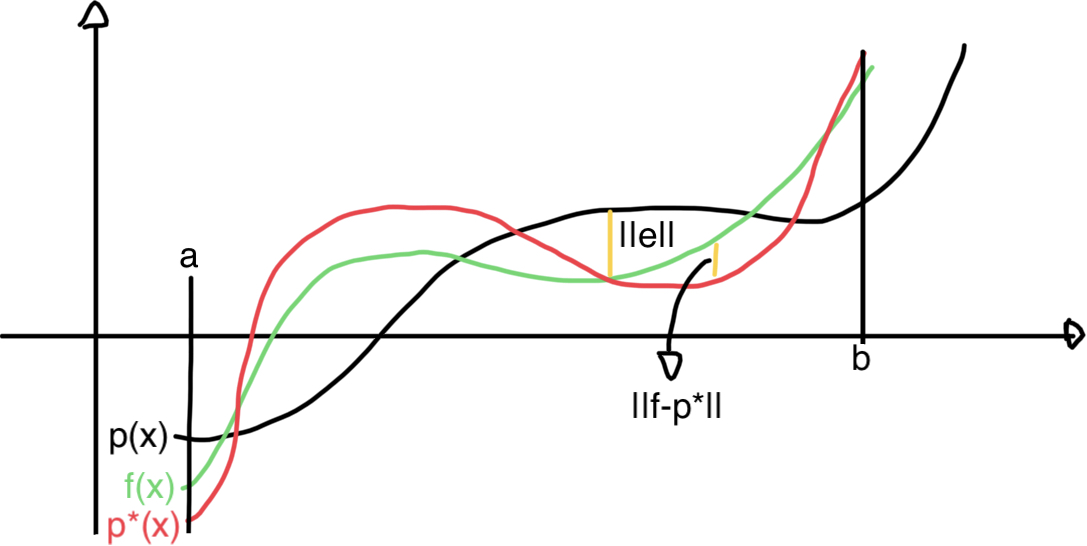
\includegraphics[width=0.75\textwidth]{immagini/esempioGrafMiglApprox.jpg}
    \caption{Esempio grafico della approssimazione $p$ e dell'errore (\ref{eq:errMiglAppross}) conseguente.}\label{fig:esempioGrafMiglApprox}
\end{figure}

Dato $p(x)$, polinomio interpolante $f(x)$ di grado $n$, è trattato come l'errore di interpolazione sia legato all'errore di migliore approssimazione (\ref{eq:errMiglAppross}). A questo scopo è definito $\boldsymbol{||e||=||f-p||}$, ovvero l'\textbf{errore massimo di interpolazione}.

\begin{theorem}\label{th:approxErrMiglApprox}\footnote{Slide 8 PDF 20, Teorema 4.7 PG 90}
    Sia $p*(x)$ il polinomio di migliore approssimazione di grado $n$ di $f(x)$, allora, per l'errore di interpolazione (\ref{eq:defErrInter}), vale:
    \begin{equation}\label{eq:errInterpMiglApprox}
        ||e||\leq (1+\boldsymbol{\Lambda_n})\overbrace{||f-p^*||}^{\footnotemark},
    \end{equation}
    dove $\boldsymbol{\Lambda_n}$ è la costante di Lebesque, definita sulle ascisse di interpolazione.
\end{theorem}\footnotetext{Quantità che tende a 0 quando $n$ cresce (lentamente in generale).}
\begin{proof}
Considerando $p^*\in\Pi_n$:
    \begin{equation*}
        \begin{matrix}
            ||e||&\overset{\footnotemark}{=}&||f-p^*+p^*-p||\\
            &\leq& ||f-p^*||+||p^*-p||\\
            &\leq& ||f-p^*||+\Lambda_n||f-p^*||
            &=&(1+\Lambda_n)||f-p^*||.
        \end{matrix}
    \end{equation*}\footnotetext{Aggiunto il polinomio $p^*$ per il quale vale la diseguaglianza triangolare.}
    Su $p^*(x)$ sono possibili le seguenti considerazioni:
    \begin{itemize}
        \item coincide con il suo polinomio interpolante sulle $n+1$ ascisse sul quale è definito $p(x)$;
        \item può essere interpretato come una perturbazione $\widehat f(x)$ di $f(x)$.
    \end{itemize}
\end{proof}

È necessaria un'approssimazione dell'errore di migliore approssimazione (\ref{eq:errMiglAppross}) in quanto l'errore crescerà al crescere di $n$, se la costante di Lebesque diverge esponenzialmente. Per questo è fornita una maggiorazione per (\ref{eq:errMiglAppross}), introducendo il modulo di continuità di una funzione.

\begin{definition}[Modulo di continuità di una funzione]
    Data $f\in C^{(0)}[a,b]$ è definito il modulo di continuità di $f$, per $h>0$ (variazione), come:
    \begin{equation}\label{eq:modCont}
        \boldsymbol{\omega(f;h)}=\left\{\underset{x,y\in [a,b]}{\sup}|f(x)-f(y)|:\; |x-y|\leq h\right\}.
    \end{equation}
\end{definition}

\begin{figure}
    \centering
    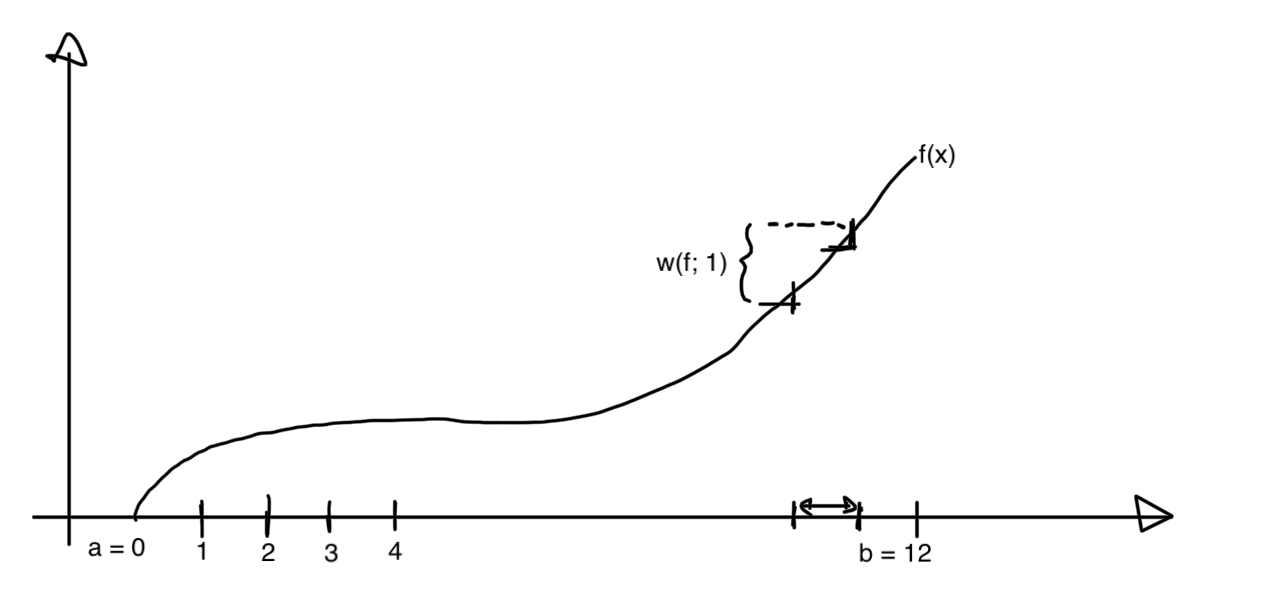
\includegraphics[width=0.75\textwidth]{immagini/modContEs.png}
    \caption{Esempio modulo di continuità. $\omega (f;1)$ è la massima distanza sul grafico di $f$ tra i punti.}\label{fig:modContEs}
\end{figure}

\begin{theorem}\label{th:modContInf}\footnote{Slide 10 PDF 20, primo punto PG 91}
    Se $f\in C^{(0)}[a,b]\Rightarrow\omega (f;h)\rightarrow 0$, per $h\rightarrow 0$.
\end{theorem}

\begin{definition}[Polinomio di migliore approssimazione]
    Data $f\in C^{(0)}[a,b]$ allora è definito polinomio di migliore approssimazione di grado $n$ di $f$ su $[a,b]$:
    \begin{equation}
        p^* \overset{\footnotemark}{=} \underset{p\in\Pi_n}{\arg\min}||f-p||.
    \end{equation}
\end{definition}

\footnotetext{$\underset{x\in X}{\arg\min}f(x)=\{x\,|\,\forall y : f(y)\geq f(x)\}$. In altre parole, è l'insieme dei valori di $x$ per i quali $f(x)$ raggiunge il suo più alto valore $M$.}

Dato $p(x)\in\Pi_n$, ovvero un polinomio interpolante $f(x)$ su $n+1$ ascisse in $[a,b]$, valgono i due seguenti risultati.

\begin{theorem}[Jackson]\label{th:Jackson}\footnote{Slide 10 PDF 20, Teorema 4.8 PG 91}
    Se $f\in C^{(0)}[a,b]$ e $p^*$ è il suo polinomio di migliore approssimazione di grado $n$, allora $\exists\, \alpha$, indipendente da $n$, tale che:
    \begin{equation}\label{eq:approxJackson}
        ||f-p^*||\leq \alpha\cdot\omega\left(f;\frac{\overset{\footnotemark}{b-a}}{\underset{\footnotemark}{n}}\right).
    \end{equation}
\end{theorem}

\addtocounter{footnote}{-1}
\footnotetext{Ampiezza dell'intervallo sul quale approssimiamo $f$.}

\stepcounter{footnote}
\footnotetext{Grado del polinomio di migliore approssimazione. Più questo cresce più $\omega\rightarrow 0$, quindi $||f-p||>0$.}

\begin{corollary}
    Se $f\in C^{(0)}[a,b]$, allora
    \begin{equation*}
        ||f-p^*_n||\rightarrow 0,\quad n\rightarrow\infty,
    \end{equation*}
    essendo $\{p^*_n\}$ la successione dei problemi di migliore approssimazione di $f$ di grado $n$.
\end{corollary}


È possibile affermare che esiste una relazione fra l'errore nell'approssimazione polinomiale ed il condizionamento del problema (dato il Teorema di Jackson).

\begin{corollary}\footnote{Slide 10 PDF 20, PG 91. Dalle (\ref{eq:errInterpMiglApprox})-(\ref{eq:approxJackson}) vale quanto segue.}
    $\forall n\geq 0$, data una funzione $f(x)$ generica, $p(x)$ il polinomio interpolante di grado $n$ su $n+1$ ascisse assegnate e $\Lambda_n$ la corrispondente costante di Lebesque, vale che:
    \begin{equation}\label{eq:maggErrMiglAprrox}
        \boxed{||e||=||f-p||\leq\underset{\footnotemark}{\alpha}\underbrace{(1+\Lambda_n)\,\omega\left(f;\frac{b-a}{n}\right)}_{\footnotemark}}.
    \end{equation}
\end{corollary}

\addtocounter{footnote}{-1}
\footnotetext{Non dipende da $n$, ovvero il grado del polinomio approssimante.}

\stepcounter{footnote}
\footnotetext{Definita nella dimostrazione del Teorema \ref{th:approxErrMiglApprox}.}

Quest'utlima espressione sarà utile per introdurre nuovi metodi di interpolazione. Inoltre, è necessario che la costante $\Lambda_n$ non cresca più rapidamente della quantità per la quale è moltiplicata, ma tenda a 0, al crescere del numero di ascisse di interpolazione.

\begin{remark}\footnote{Slide 10 PDF 20.}
    Al crescere del numero delle ascisse di interpolazione $(n+1)$ è necessario fare in modo che $\Lambda_n$ cresca in modo ottimale, affinché $||e||$ diminuisca.
\end{remark}

\subsection{Ascisse di Chebyshev}\label{ssec:AscCheb}\footnote{PDF 21, PG 91-93.}
Le Sezioni \ref{ssec:errInter} e \ref{ssec:condProbApproxfun} sono riassumibili nei seguenti punti:
\begin{itemize}
    \item $\Lambda_n$ è indipendente dal particolare intervallo considerato; cresce esponenzialmente con $n$ se sono utilizzate ascisse equidistanti, altrimenti ha una crescita moderta (quella ottimale è di tipo logaritmico) rispetto ad $n$; \footnote{$n$ è il grado del polinomio interpolante.}
    \item Data la maggiorazione $||e||\leq \frac{\overbrace{||f^{(n+1)}||}^{\footnotemark}}{(n+1)!}||\omega_{n+1}||,\text{ con } \omega_{n+1}(x)=\prod_{j=0}^n(x-x_j)$, è necessario capire come questa sia collegata con (\ref{eq:maggErrMiglAprrox}). 
\end{itemize}\footnotetext{Indipendente dalle ascisse, non come $||w_{n+1}||$.}

L'obbiettivo della Sezione è  quello di scegliere le ascisse di interpolazione $x_j$ in modo da minimizzare $||\omega_{n+1}||$. Per fare questo è necessario rendere la costante di Lebesque piccola o almeno con una precisione accettabile.

Considerando l'intervallo di riferimento $\boldsymbol{[-1,1]}$, è necessario scegliere le ascisse $x_0,\hdots,x_n$ in modo tale da risolvere il problema del \textbf{minmax}, ovvero il seguente: \footnotemark
\begin{equation}\label{eq:minmax}
    \underset{a=-1\leq x_0<\hdots<x_n\leq 1=b}{\min}||w_{n+1}||=\boldsymbol{\underset{a=-1\leq x_0<\hdots<x_n\leq 1=b}{\min}\quad\underset{-1\leq x\leq 1}{\max}|}\overbrace{\boldsymbol{w_{n+1}(x)}}^{\footnotemark}\boldsymbol|,
\end{equation}
con $w_{n+1}(x)$ calcolata come in (\ref{polBaseNewt2}), ovvero $\prod_{j=0}^n(x-x_j)$.
\addtocounter{footnote}{-1}
\footnotetext{Slide 5 PDF 21, PG 91.}

\stepcounter{footnote}
\footnotetext{Polinomio monico che ha come radici le ascisse, rispetto alle quali è svolta la minimizzazione.}

A questo scopo è introdotta la seguente Definizione:

\begin{definition}[Polinomi di Chebyshev di I specie]\label{th:polChebIsp}
    Assunto $x\in [-1,1]$, la \textbf{famiglia di polinomi di Chebyshev di I specie} è definita come segue:
    \begin{equation}\label{eq:polChebISp}
        \begin{cases}
        T_0(x) \equiv 1;\\
        T_1(x) = x;\\
        T_{k+1}(x) = 2x\cdot T_k(x)-T_{k-1}(x),\;\; k\geq 1.
        \end{cases}
    \end{equation}
\end{definition}

\begin{example}
    \begin{equation*}
        \begin{matrix}
            T_2 &=& 2x \cdot \equaltoup{x}{T_1(x)} - \equaltoup{1}{T_0(x)} &=& 2x^2-1,\\
            T_3(x) &=& 2x\cdot T_2(x)-T_1(x)&=&2x(2x^2-1)-x&=& 4x^3-2x-x &=& 4x^3-3x,\\
            \vdots
        \end{matrix}
    \end{equation*}
    \qed
\end{example}

Alcune proprietà dei polinomi di Chebyshev di I specie sono le seguenti:
\begin{itemize}
    \item [P1)] $\boldsymbol{T_k(x)}$ è un \textbf{polinomio di grado esatto} $\boldsymbol k,\,\forall k=0,1,\hdots$;
    \item[P2)]\footnotemark Il coefficiente principale di $\boldsymbol{T_k(x)}$ è $\boldsymbol{2^{k-1}},\,\forall\,k=1,2,\hdots$;
    \footnotetext{A cosa serve questa proprietà? Dato il polinomio $4x^2-1$, è necessario dividerlo per 4 per renderlo monico (4 è il coeficiente principale del polinomio). Data una famiglia di polinomi di grado $k$, se è necessario derivare una famiglia di polinomi monici è necessario conoscere qual è il coefficiente principale di ciascuno di loro.}
    \item[P3)]\footnotemark I polinomi $\boldsymbol{\left\{\widehat T_k\right\}_{k\geq 0}}$ definiti come
    \begin{equation*}
        \begin{cases}
            \widehat T_0(x)=T_0\equiv 1,\\
            \widehat T_k(x) =\boldsymbol{2^{1-k}}\, T_k(x),\;\; k=1,2,\hdots
        \end{cases}
    \end{equation*}
    sono una \textbf{famiglia di polinomi monici} (perché $2^{1-k}$ è il reciproco del precedente coefficiente $2^{k-1}$);
    \footnotetext{Dati i polinomi di grado $k$ con 8 coefficienti principali, è possibile derivare da questa una famiglia di polinomi monici.}
    \item[P4)] 
    \begin{equation*}
        \forall\, k\geq 1: \widehat T_k(x)=\prod_{j=0}^{k-1}\left(x-x_j^{(k)}\right),
    \end{equation*}
    con $T_k\left(\boldsymbol{x_j^{(k)}}\right)=0,\; j=0,\hdots,k-1,\;\text{dove } \boldsymbol{x_j^{(k)}}$ sono le \textbf{radici} di $\boldsymbol{T_k(x)}$. \footnote{Se le radici $x_j^{(k)}$ fossero tutte distinte e nell'intervallo $[-1,1]$, allora per il polinomio $\widehat T_k(x)$ è possibile scegliere un'ascissa di interpolazione.}
\end{itemize}

\begin{remark}\label{re:ver1&2}\footnote{Slide 7 PDF 21.}
    Considerata $\widehat T_{n+1}(x)=\prod_{j=0}^n\left(x-x_j^{(n+1)}\right)$, dove $x_j^{(n+1)},\; j=0,\hdots,n$, sono le radici di $T_{n+1}(x)$ e date le seguenti condizioni sulle radici:
    \begin{enumerate}
        \item $x_i^{(n+1)}\neq x_j^{(n+1)},\quad i\neq j,\; i,j=0,\hdots,n;$ \footnote{Definisce le ascisse distinte.}
        \item $x_j^{(n+1)}\in [-1,1],\quad \forall j=0,\hdots,n;$ \footnote{Definisce le ascisse in un intervallo.}
    \end{enumerate}
    allora è possibile sceglierle come ascisse di interpolazione, per cui:
    \begin{equation*}
        \boldsymbol{\omega_{n+1}\equiv\widehat T_{n+1}=\prod_{j=0}^{n}\left(x-x_j^{(n+1)}\right)}.
    \end{equation*}
    Per verificare che 1. e 2. siano soddisfatte, sarà ottenuta un'espressione esplicita delle ascisse stesse. Poiché $x\in [-1,1]$, è posto $x=\cos(\theta),\, \theta\in [0,\pi],$ allora $\theta=\arccos{x}$ (vedere Figura \ref{fig:cosThetaChebyshev}).
\end{remark}

\begin{figure}
    \centering
    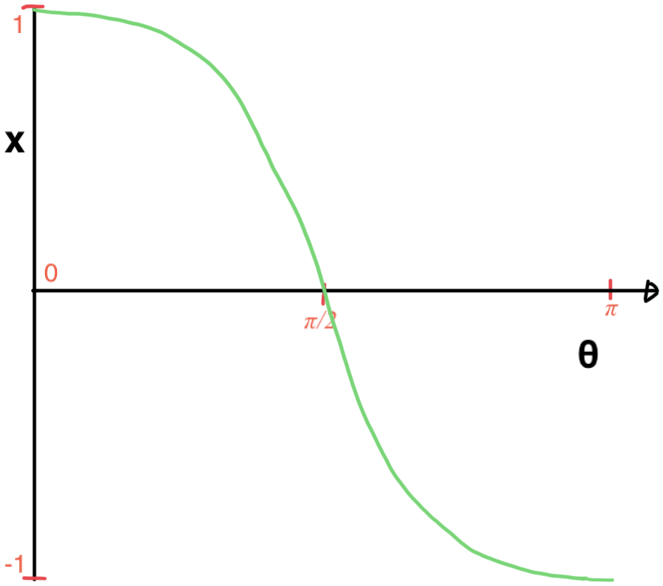
\includegraphics[width=0.35\textwidth]{immagini/cosThetaChebyshev.png}
    \caption{Grafico osservazione \ref{re:ver1&2}.}\label{fig:cosThetaChebyshev}
\end{figure}

\begin{itemize}
    \item[P5)] Se $\boldsymbol{x=\cos\theta}\Rightarrow T_k(x)=T_k(\cos\theta)=\cos{k\theta}\;\footnotemark.$
    \footnotetext{Polinomio di Chebyschev, se $x$ è parametrizzata in modo idoneo.}
    \begin{proof}
        È svolta per induzione su $k$.
        \begin{equation*}
            \begin{matrix}
                k=0&\Rightarrow& T_0(x) &=& T_0(\cos\theta) &=& \cos{(0\cdot\theta)} &\equiv& 1,\\
                k=1 &\Rightarrow& T_1(x) &=& T_1(\cos\theta) &=& \cos\theta &=& x,
            \end{matrix}
        \end{equation*}
        supposto vero per $k$ e $k-1$ è dimostrato per $k+1$ ciò che segue:
        \begin{equation*}
            \begin{matrix}
                \boldsymbol{T_{k+1}(x)}&\boldsymbol =& 2x\,T_k(x)-T_{k-1}(x) &=& 2cos\theta\cdot\cos{(k\theta)}-\cos{((k-1)\theta)}\\
                &=&2cos\theta\cdot\cos{(k\theta)}-\cos\theta\cdot\cos{(k\theta)}-\sin\theta\sin{(k\theta)} &=& \cos\theta\cdot\cos{(k\theta)}-\sin\theta\cdot\sin{(k\theta)}\\
                &&&=&\boldsymbol{\cos{((k+1)\,\theta)}}
            \end{matrix}
        \end{equation*}
    \end{proof}
    \item[P6)]\footnotemark $||T_k||=\underset{\theta\in [0,\pi]}{\max}|\cos{k\theta}|
    \underset{\footnotemark}{=} 1,\;\forall k\geq 0$;
    \addtocounter{footnote}{-1}
    \footnotetext{Deriva dalla precedente proprietà.}
    \stepcounter{footnote}
    \footnotetext{In $[0,\pi]$ il massimo vale 1.}
    \item[P7)]$||\widehat T_k||=2^{1-k}||T_k||=2^{1-k},\;\forall k\geq 1$, con $\widehat T_k$ detto polinomio monicizzato;
    \item[P8)] Gli zeri di $T_k(x)$ sono ottenuti imponendo che $x=\cos\theta,\;\theta\in [0,\pi]$ e 
    \begin{equation*}
        \begin{matrix}
            T_k(x)&=&T_k(\cos\theta)=\cos{(k\theta)}=0\\
            &\underset{\footnotemark}{\Rightarrow}& k\theta=\frac{\pi}{2}+i\,\pi\\
            &\Rightarrow&\theta =\frac{(2i+1)\pi}{2k},\, \boldsymbol{i=0,\hdots,k-1}\\
            &\Rightarrow& x_i^{(k)} = \cos{\left(\frac{2i+1}{2k}\pi\right)},\, i=0,\hdots,k-1.
        \end{matrix}
    \end{equation*}\footnotetext{$\cos{(k\theta)}$ si annulla per $k\theta$ come segue.}
    con le ascisse risultanti reali, distintinte tra loro e appartenenti a $(-1,1)$.
\end{itemize}

\begin{definition}[Ascisse di Chebyshev]\footnote{Slide 10 PDF 21, TH 4.9 PG 92.}
    Dato il polinomio interpolante $f$ di grado $n$, le ascisse di Chebyshev sono definite come
    \begin{equation}\label{eq:ascisseChebyshev}
        x_i=\cos{\left(\frac{(2i+1)\pi}{2(n+1)}\right)},\quad i=0,\hdots,n,
    \end{equation}
    le quali sono le radici di $\widehat T_{n+1}(x)$.
\end{definition}

Dato che le ascisse di Chebyshev, appena definite, sono radici di $\widehat T_{n+1}(x)$ allora la norma
\begin{equation*}
    ||\omega_{n+1}||=||\widehat T_{n+1}||=2^{-n}\,||T_{n+1}||=2^{-n}\, 1 = \boldsymbol{2^{-n}}
\end{equation*}
è \textbf{minima} tra tutti \textbf{polinomi monici di grado} $\boldsymbol{n+1}$.\footnote{Comunque siano date le ascisse in $[-1,1]$ è ottenuto un valore più grande del $\min\max$ (\ref{eq:minmax}).} Pertanto, il polinomio di Chebyshev monicizzato di grado $n+1$ è soluzione del prodotto $\min\max$ (\ref{eq:minmax}). 

Inoltre, con la scelta delle ascisse di Chebyshev come ascisse di interpolazione è minimizzata la maggiorazione dell'errore (\ref{eq:approxJackson}), portando la costante di Lebesque a $\boldsymbol{\Lambda_n\approx\frac{2}{\pi}\log n}$. Quindi, la scelta delle ascisse di Chebyshev permette una crescita \textbf{ottimale} della costante di Lebesque, per $\boldsymbol{n\rightarrow\infty}$.

%%\vspace{6px}
%\hrule
%\vspace{-7px}
\paragraph{Ricapitolando:} Sono scelte le ascisse di interpolazione, nell'intervallo $[-1,1]$, distinte fra loro e che utilizzano la norma del polinomio monico (il quale ha come radici le ascisse del tipo $x_i$ definite in (\ref{eq:ascisseChebyshev})). 

È stato dimostrato che $||w_{n+1}||=2^{-n}$, con $n$ ottenuto attraverso le ascisse di interpolazione e le ascisse del polinomio di Chebyshev di grado $n$. 

Le ascisse del polinomio di Chebyshev di grado $n+1$ ha $n+1$ radici (necessario che un polinomio di Chebyshev di grado $n+1$ abba $n+1$ radici); con $n+1$ ascisse di interpolazione è possibile definire il polinomio interpolante di grado $n$. Quindi, se è richiesta una function per calcolare le ascisse relative al grado $n$, è neceessario ricordare di contare fino ad $n+1$ per Matlab, altrimenti sono contati $n-1$ (quindi il polinomio interpolante sarebbe di grado $n-1$).

%\vspace{3px}
%\hrule
%\vspace{6px}

\begin{figure}
    \centering
    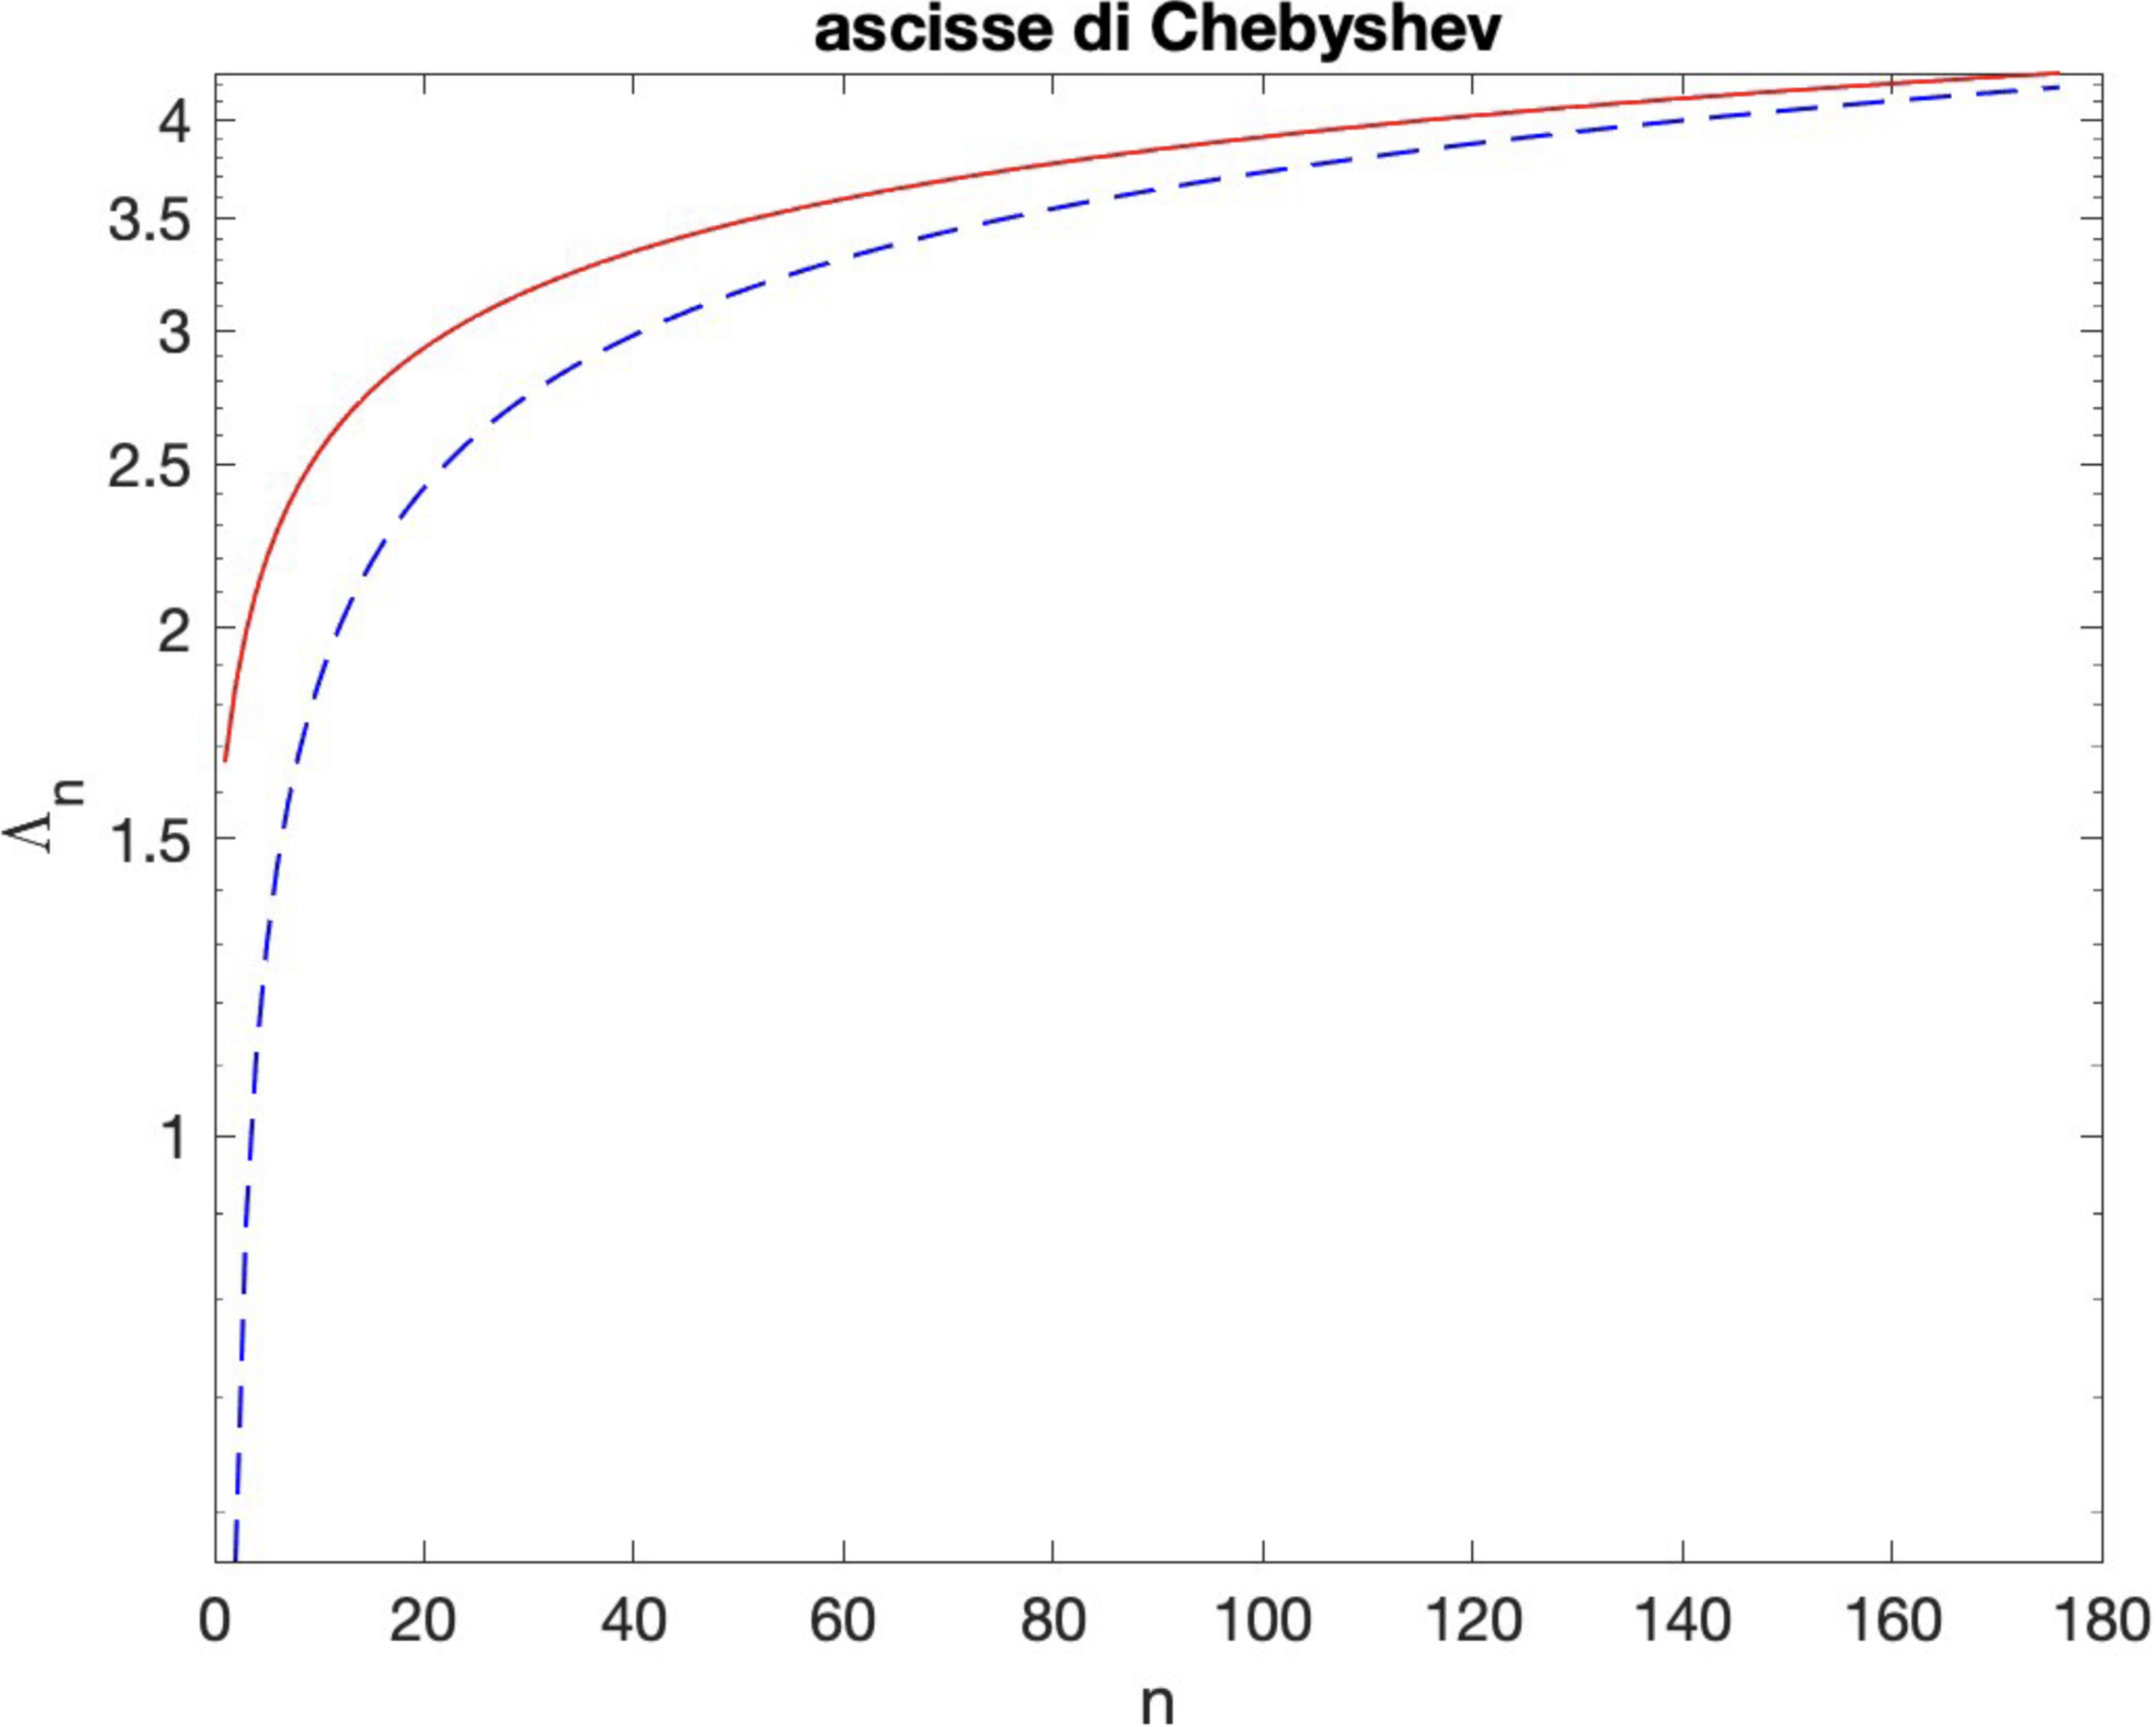
\includegraphics[width=0.5\textwidth]{immagini/graficoAscisseChebyshev.jpeg}
    \caption{Esempio di crescita di $\Lambda_n$ al crescere di $n$.}\label{fig:graficoAscisseChebyshev}
\end{figure}

Dalla Figura \ref{fig:graficoAscisseChebyshev} è possibile notare che sopra il grado 40 non vengono considerati i polinomi. Questo è dovuto al fatto che in aritmetica finita sono introdotti errori e molcondizionamento nelle operazioni. Inoltre, è introdotta la cancellazione numerica nel caso di differenza con ascisse di interpolazione sempre più vicine.

\begin{remark}
    Le ascisse di Chebyshev forniscono delle ascisse di interpolazione ottimali nell'intervallo $[-1,1]$. Per riportare ad un generico intervallo $[a,b]$ quanto descritto per (\ref{eq:ascisseChebyshev}), è possibile verificare facilmente che è sufficiente utilizzare la trasformazione lineare:
    \begin{equation*}
        x_{\boldsymbol{n-i}} =\underbrace{\frac{a+b}{2}}_{\footnotemark} + \frac{b-a}{2}\cos{\left(\frac{(2i+1)\pi}{2(\boldsymbol{n+1})}\right)},\quad i=0,\hdots,n,
    \end{equation*}
    dove è utilizzato l'indice di enumerazione in notazione $n-i$, quindi rovesciato, per ottenere le ascisse in ordine crescente. 
\end{remark}
\footnotetext{Punto medio dell'intervallo.}

Utilizzando le ascisse di Chebyshev nell'intervallo $[-5,5]$ sono ottenute le Figure \ref{fig:fRungeAscChebN=2}-\ref{fig:fRungeAscChebN=22}. Nelle figure è possibile notare che, da $n=10$ (vedere Figura \ref{fig:fRungeAscChebN=10}), la precisione di approssimazione è buona. Nella precedente approssimazione di $f(x)=\frac{1}{1+x^2}$ tramite la funzione di Runge, è possibile notare come, con 10 e più ascisse, erano presenti oscillazioni enormi agli estremi (vedere Figura \ref{fig:funzRunge_n=10} e \ref{fig:funzRunge_n=22}). Inoltre, è possibile notare come le ascisse addensate agli estremi dell'intervallo sono più vicine l'una alla altra di quanto lo siano quelle centrali.

È possibile trovare un'implementazione dell'algoritmo che calcola le ascisse di Chebyshev, per costruire il polinomio interpolante di grado $n$, su un generico intervallo $[a, b]$, nell'Algoritmo \ref{alg:cheby}.

\begin{remark}
    È necessario ricordare che al crescere del grado $n$ del polinomio interpolante, la scelta delle ascisse di interpolazione non deve fare crescere troppo la costante di Lebesque $\Lambda_n$.
\end{remark}

\begin{figure}
    \centering
    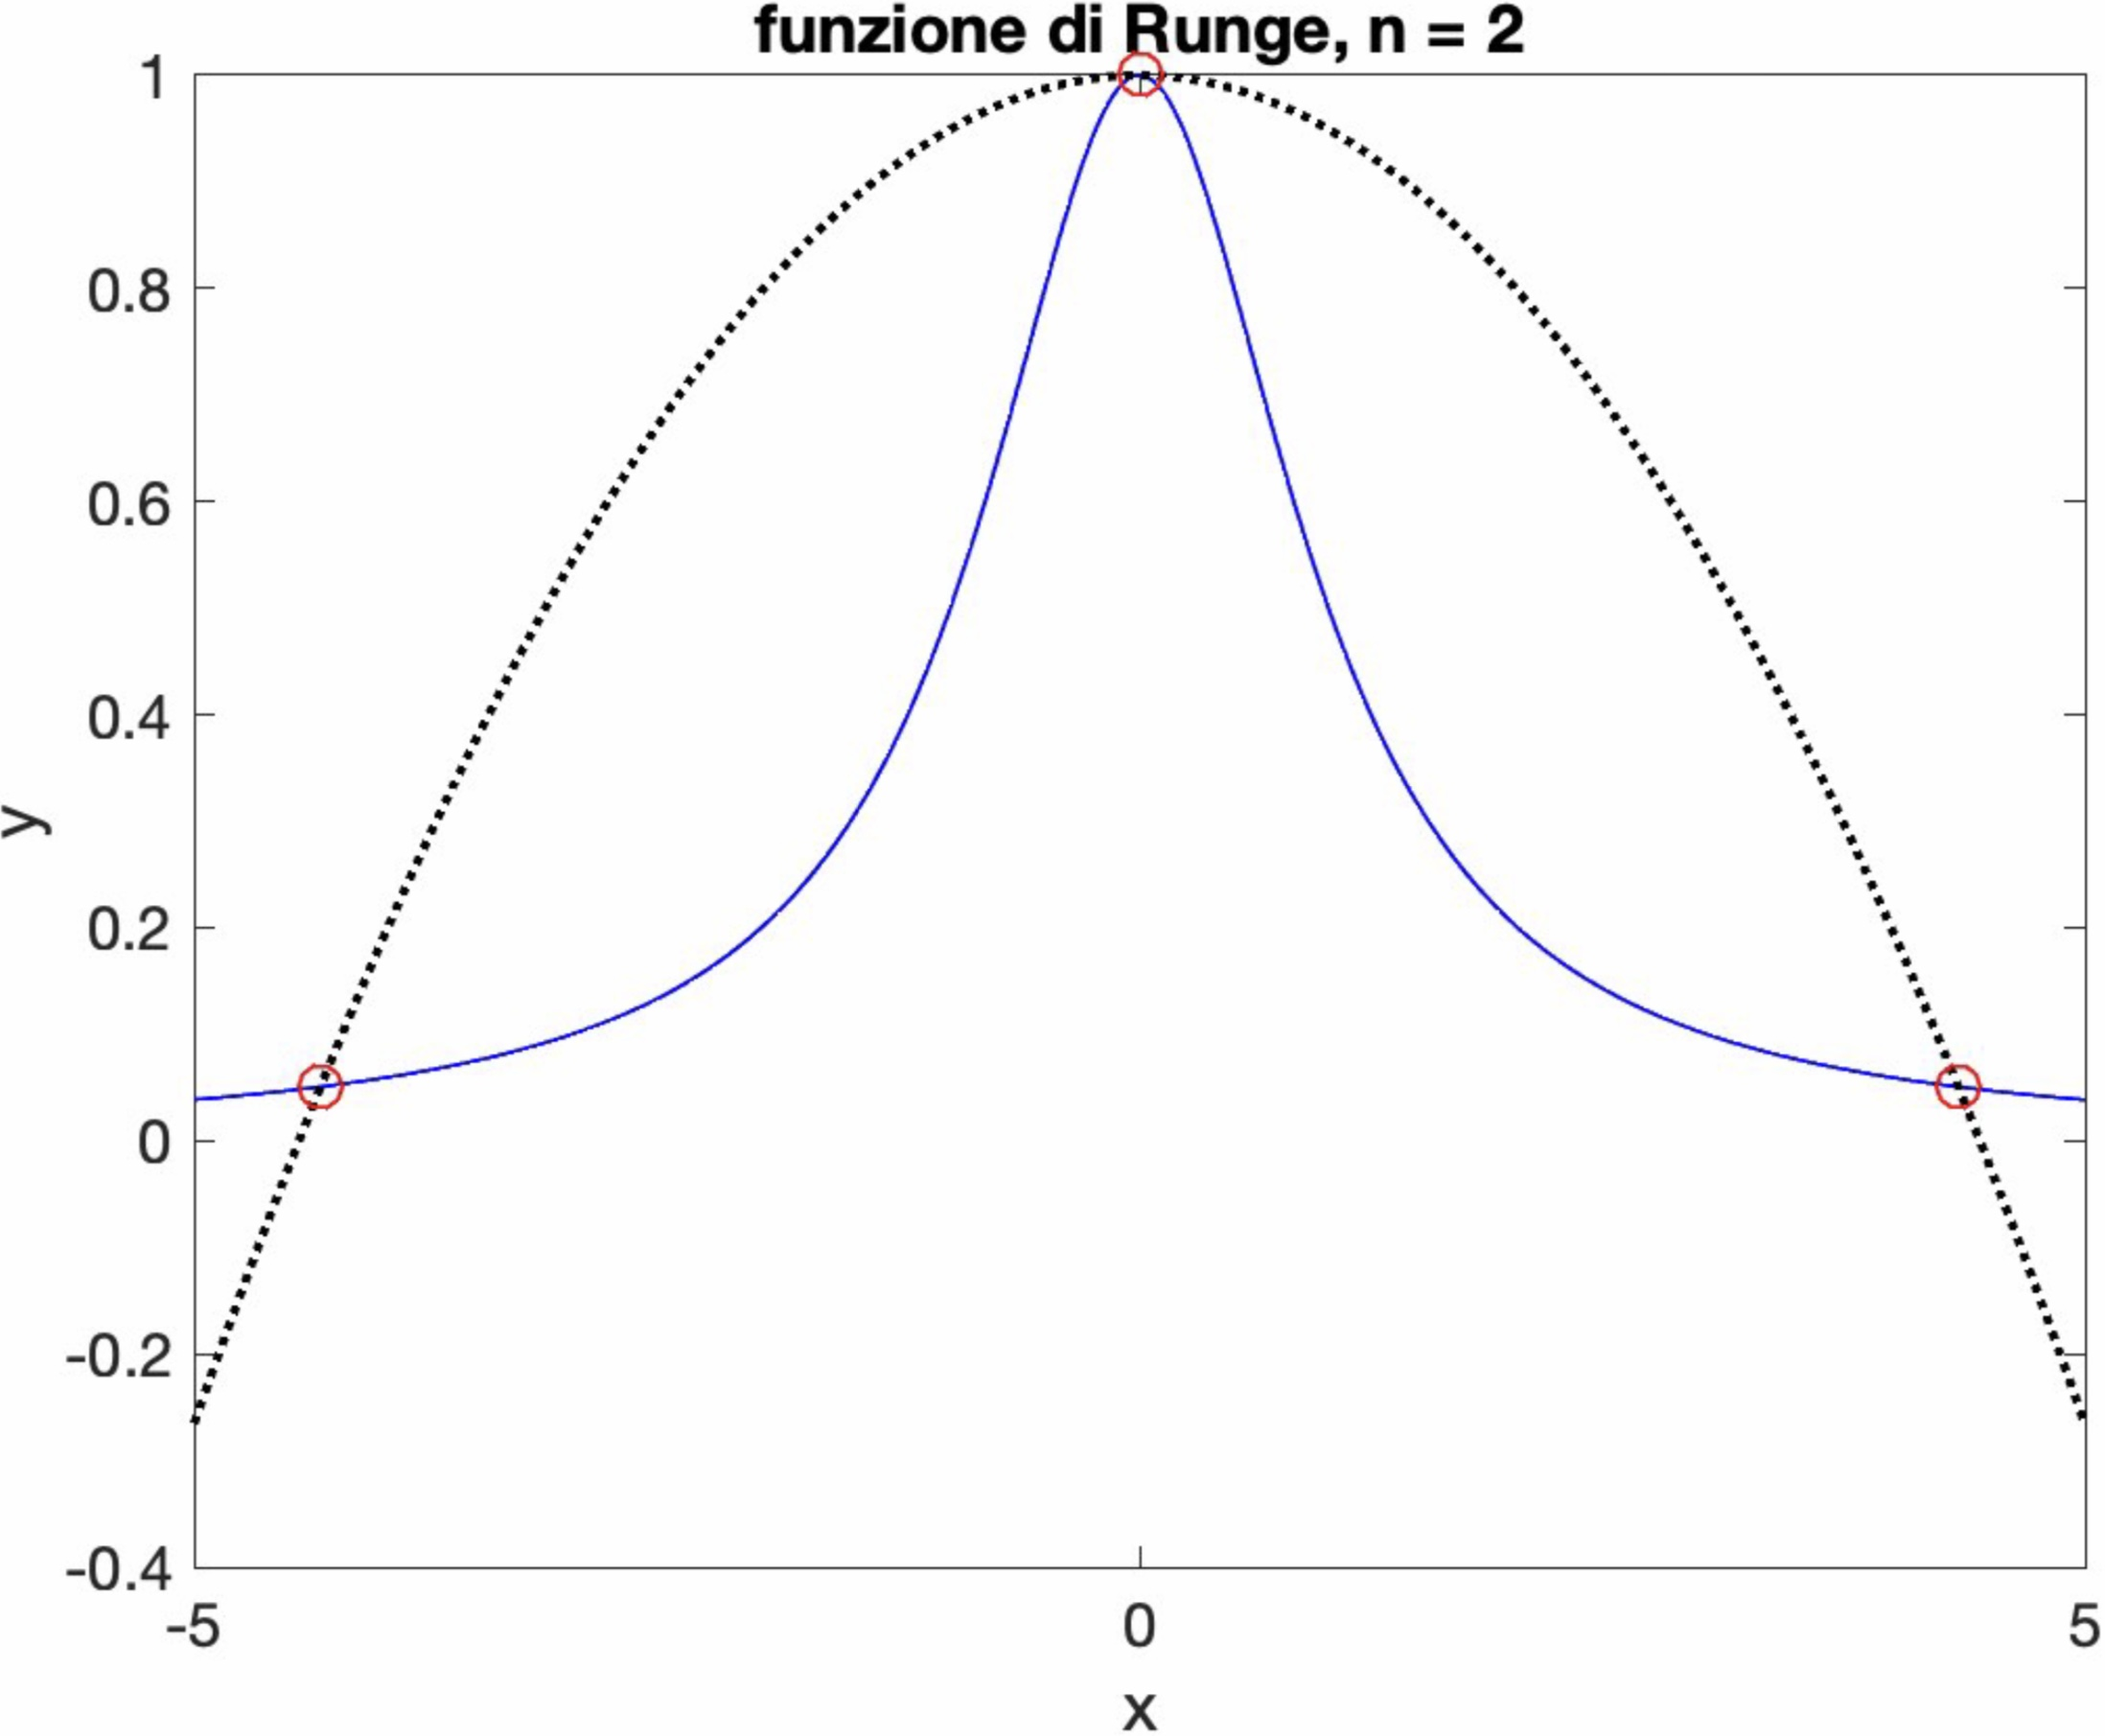
\includegraphics[width=0.5\textwidth]{immagini/fRungeAscChebN=2.jpg}
    \caption{Esempio di crescita di $\Lambda_n$ al crescere di $n$.}\label{fig:fRungeAscChebN=2}
\end{figure}

\begin{figure}
    \centering
    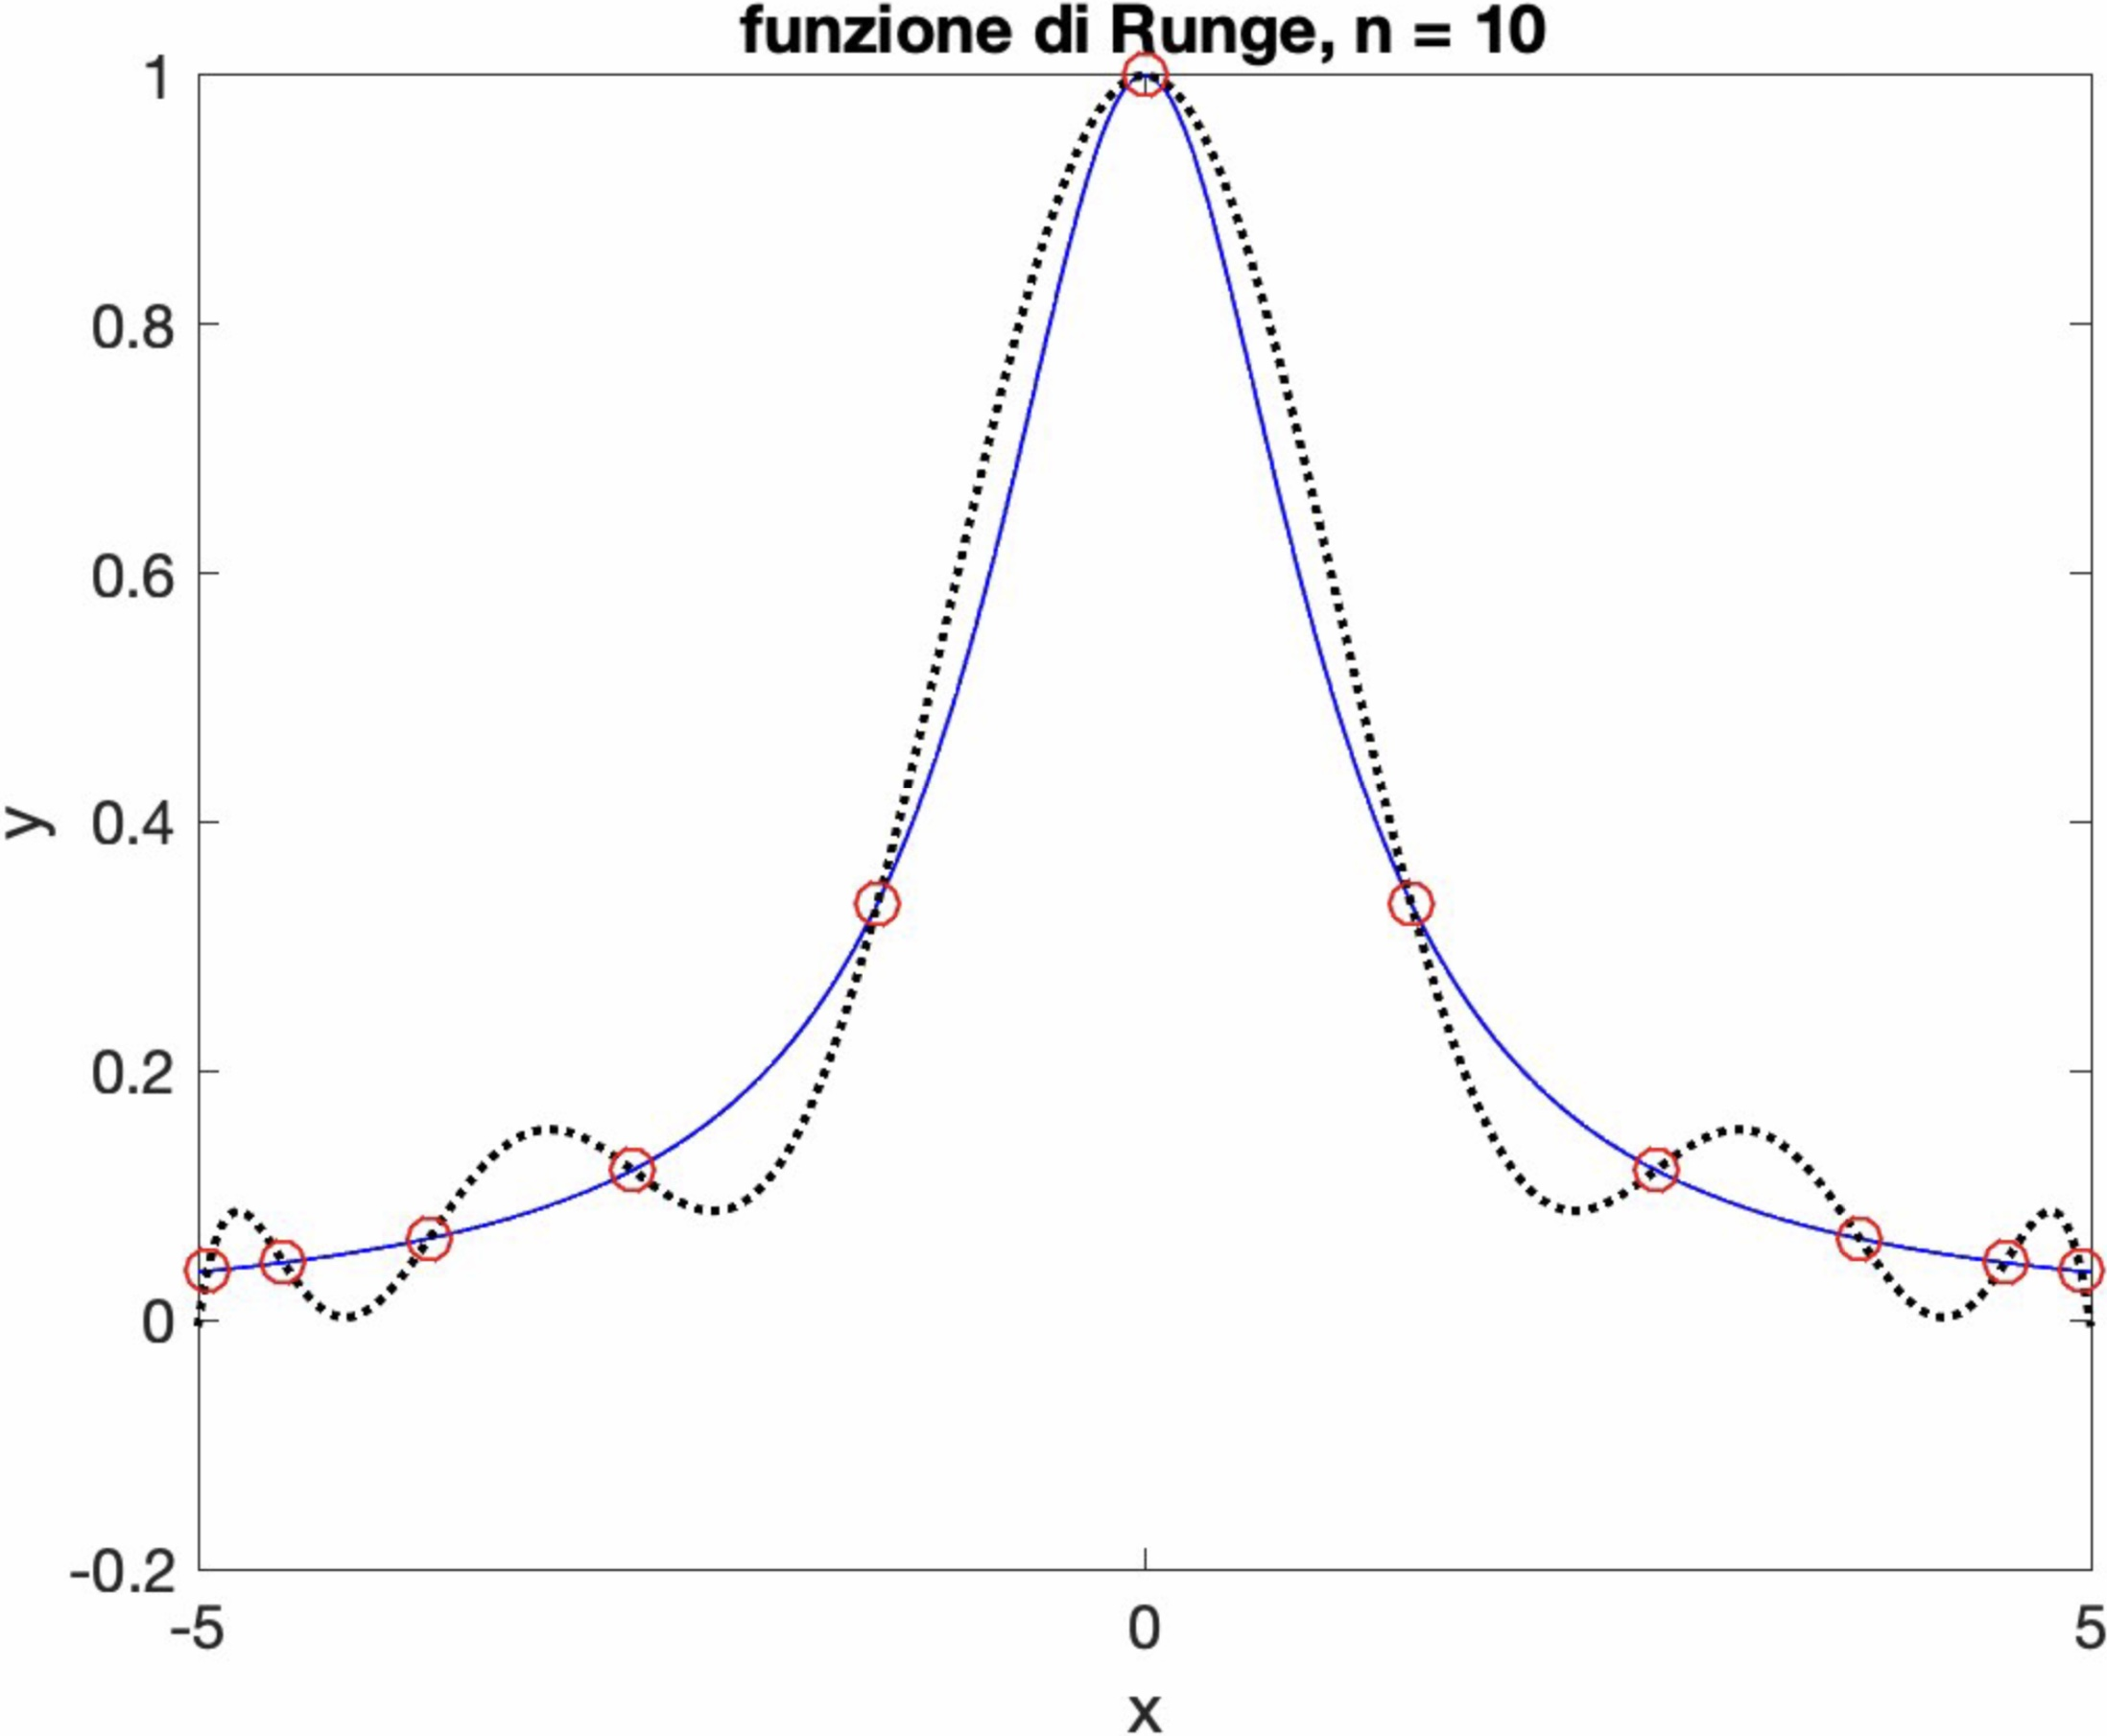
\includegraphics[width=0.5\textwidth]{immagini/fRungeAscChebN=10.jpg}
    \caption{Esempio di crescita di $\Lambda_n$ al crescere di $n$.}\label{fig:fRungeAscChebN=10}
\end{figure}

\begin{figure}
    \centering
    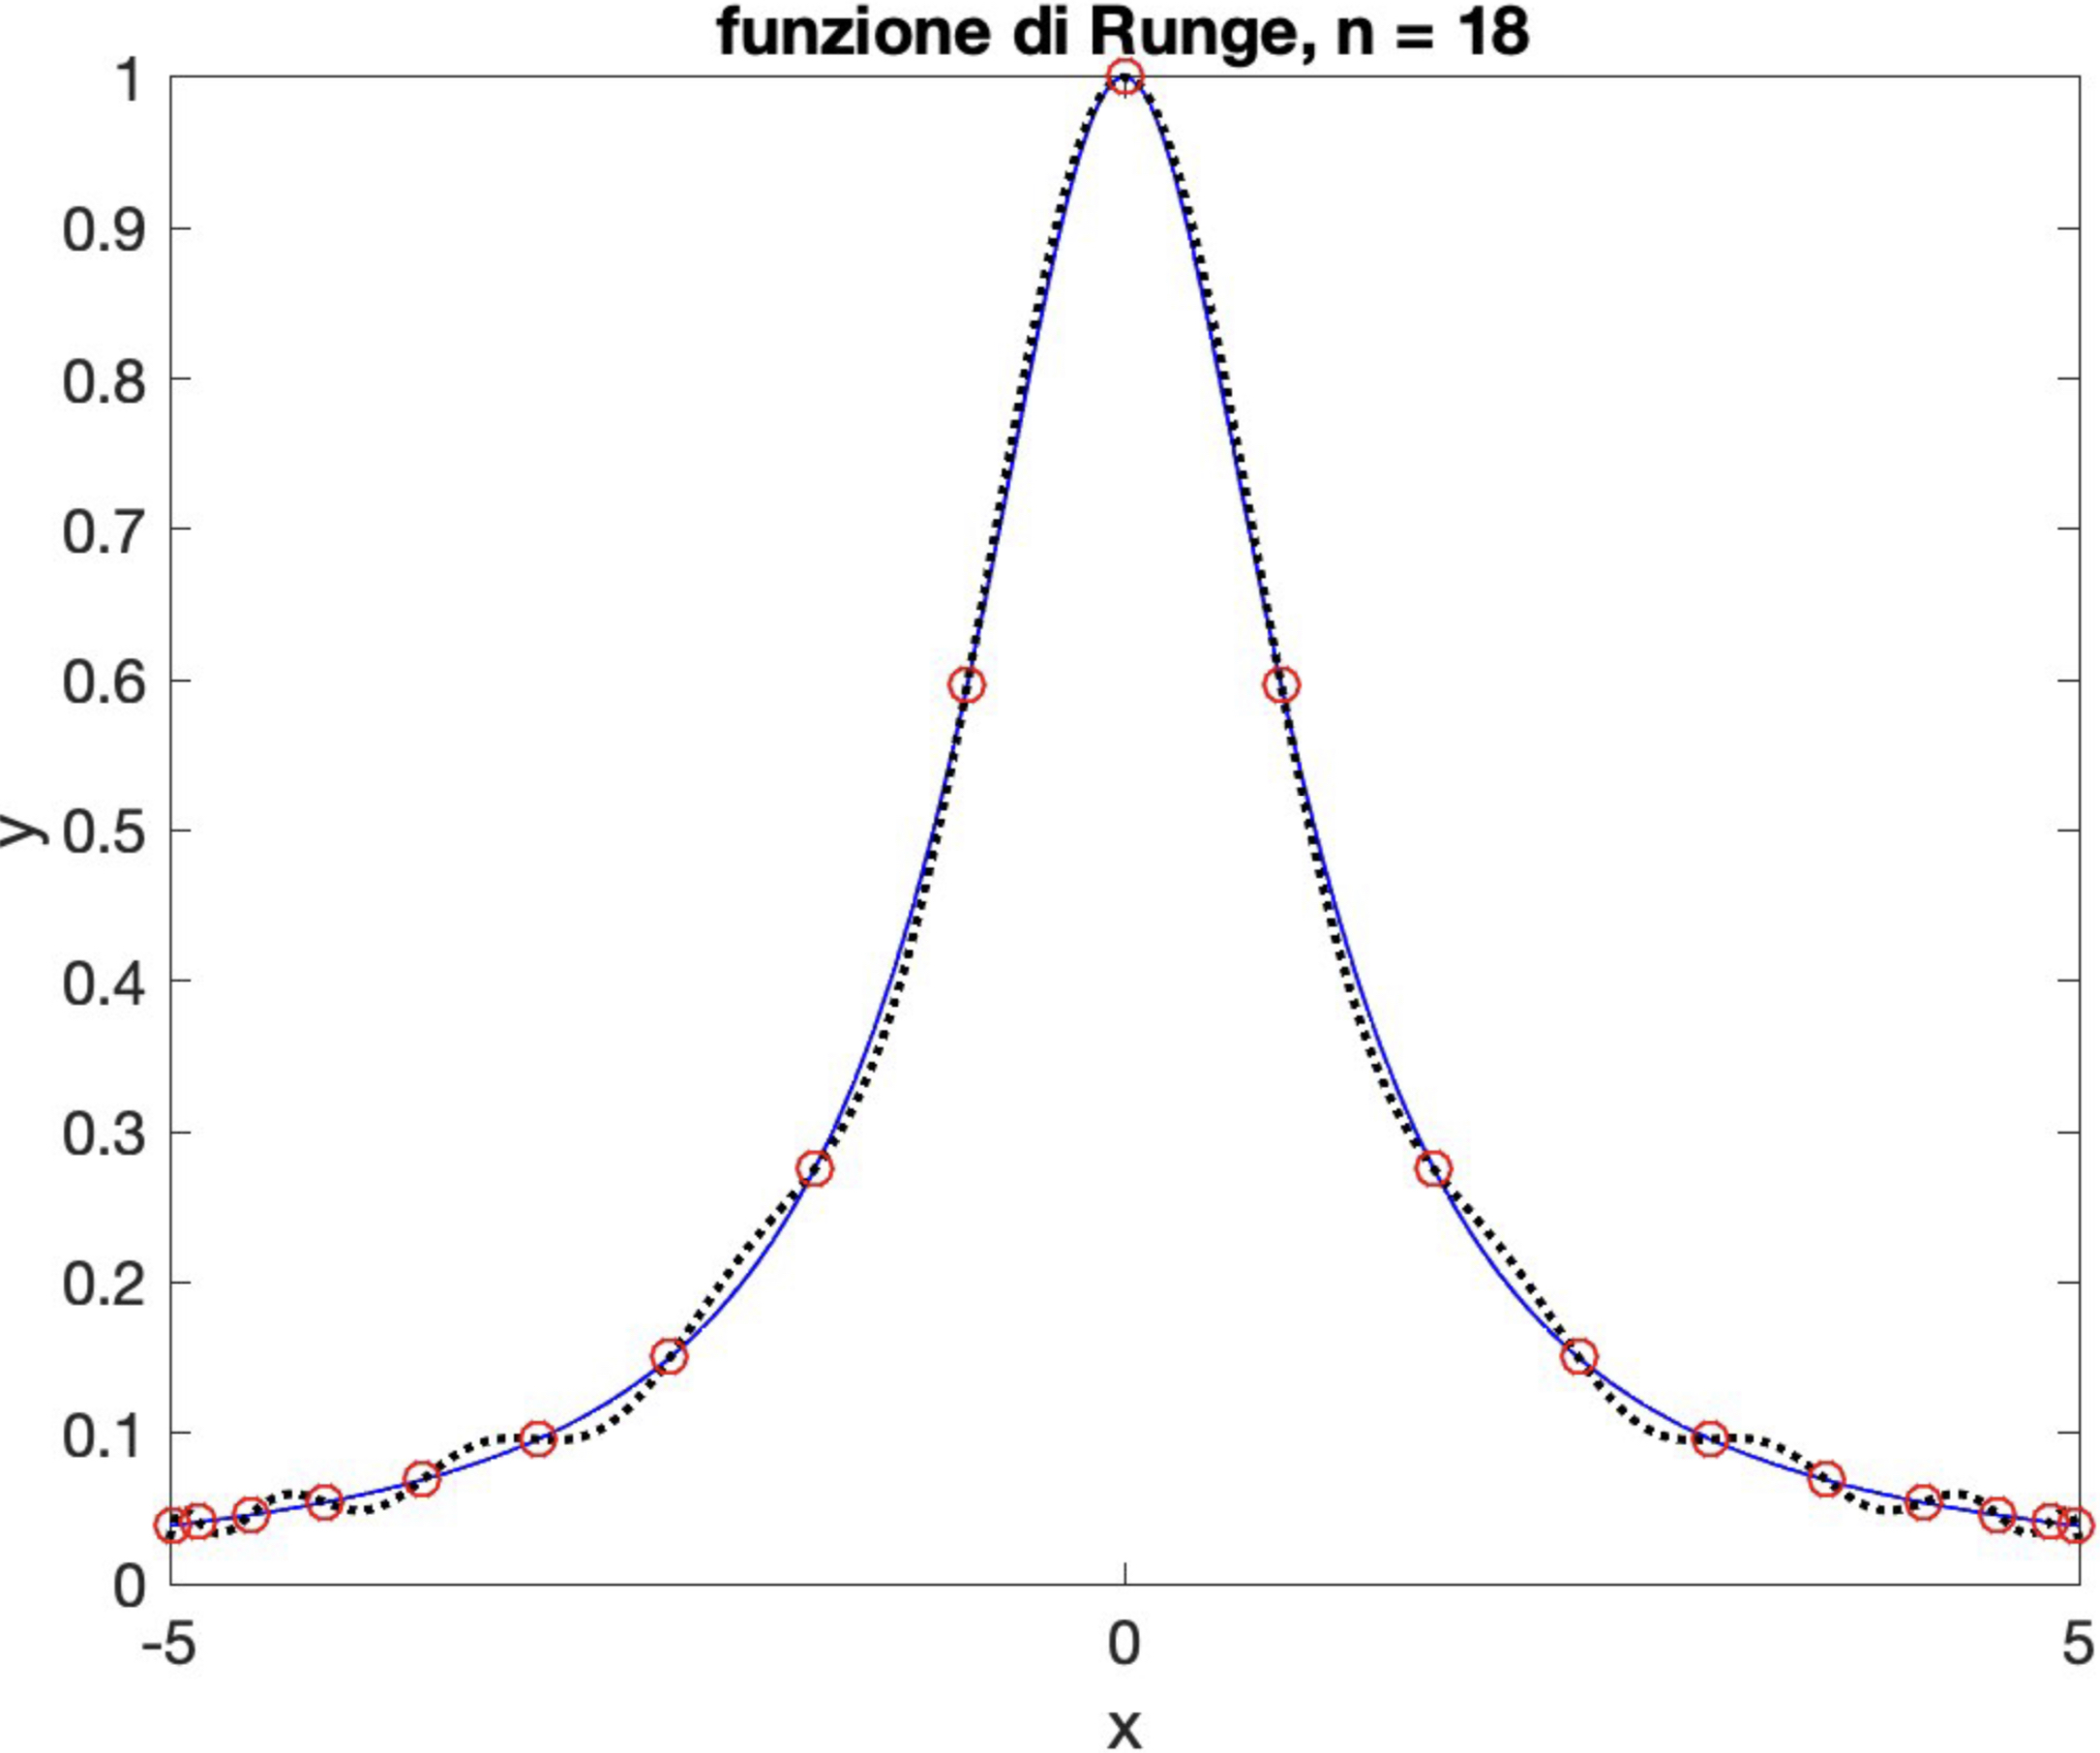
\includegraphics[width=0.5\textwidth]{immagini/fRungeAscChebN=18.jpg}
    \caption{Esempio di crescita di $\Lambda_n$ al crescere di $n$.}\label{fig:fRungeAscChebN=18}
\end{figure}

\begin{figure}
    \centering
    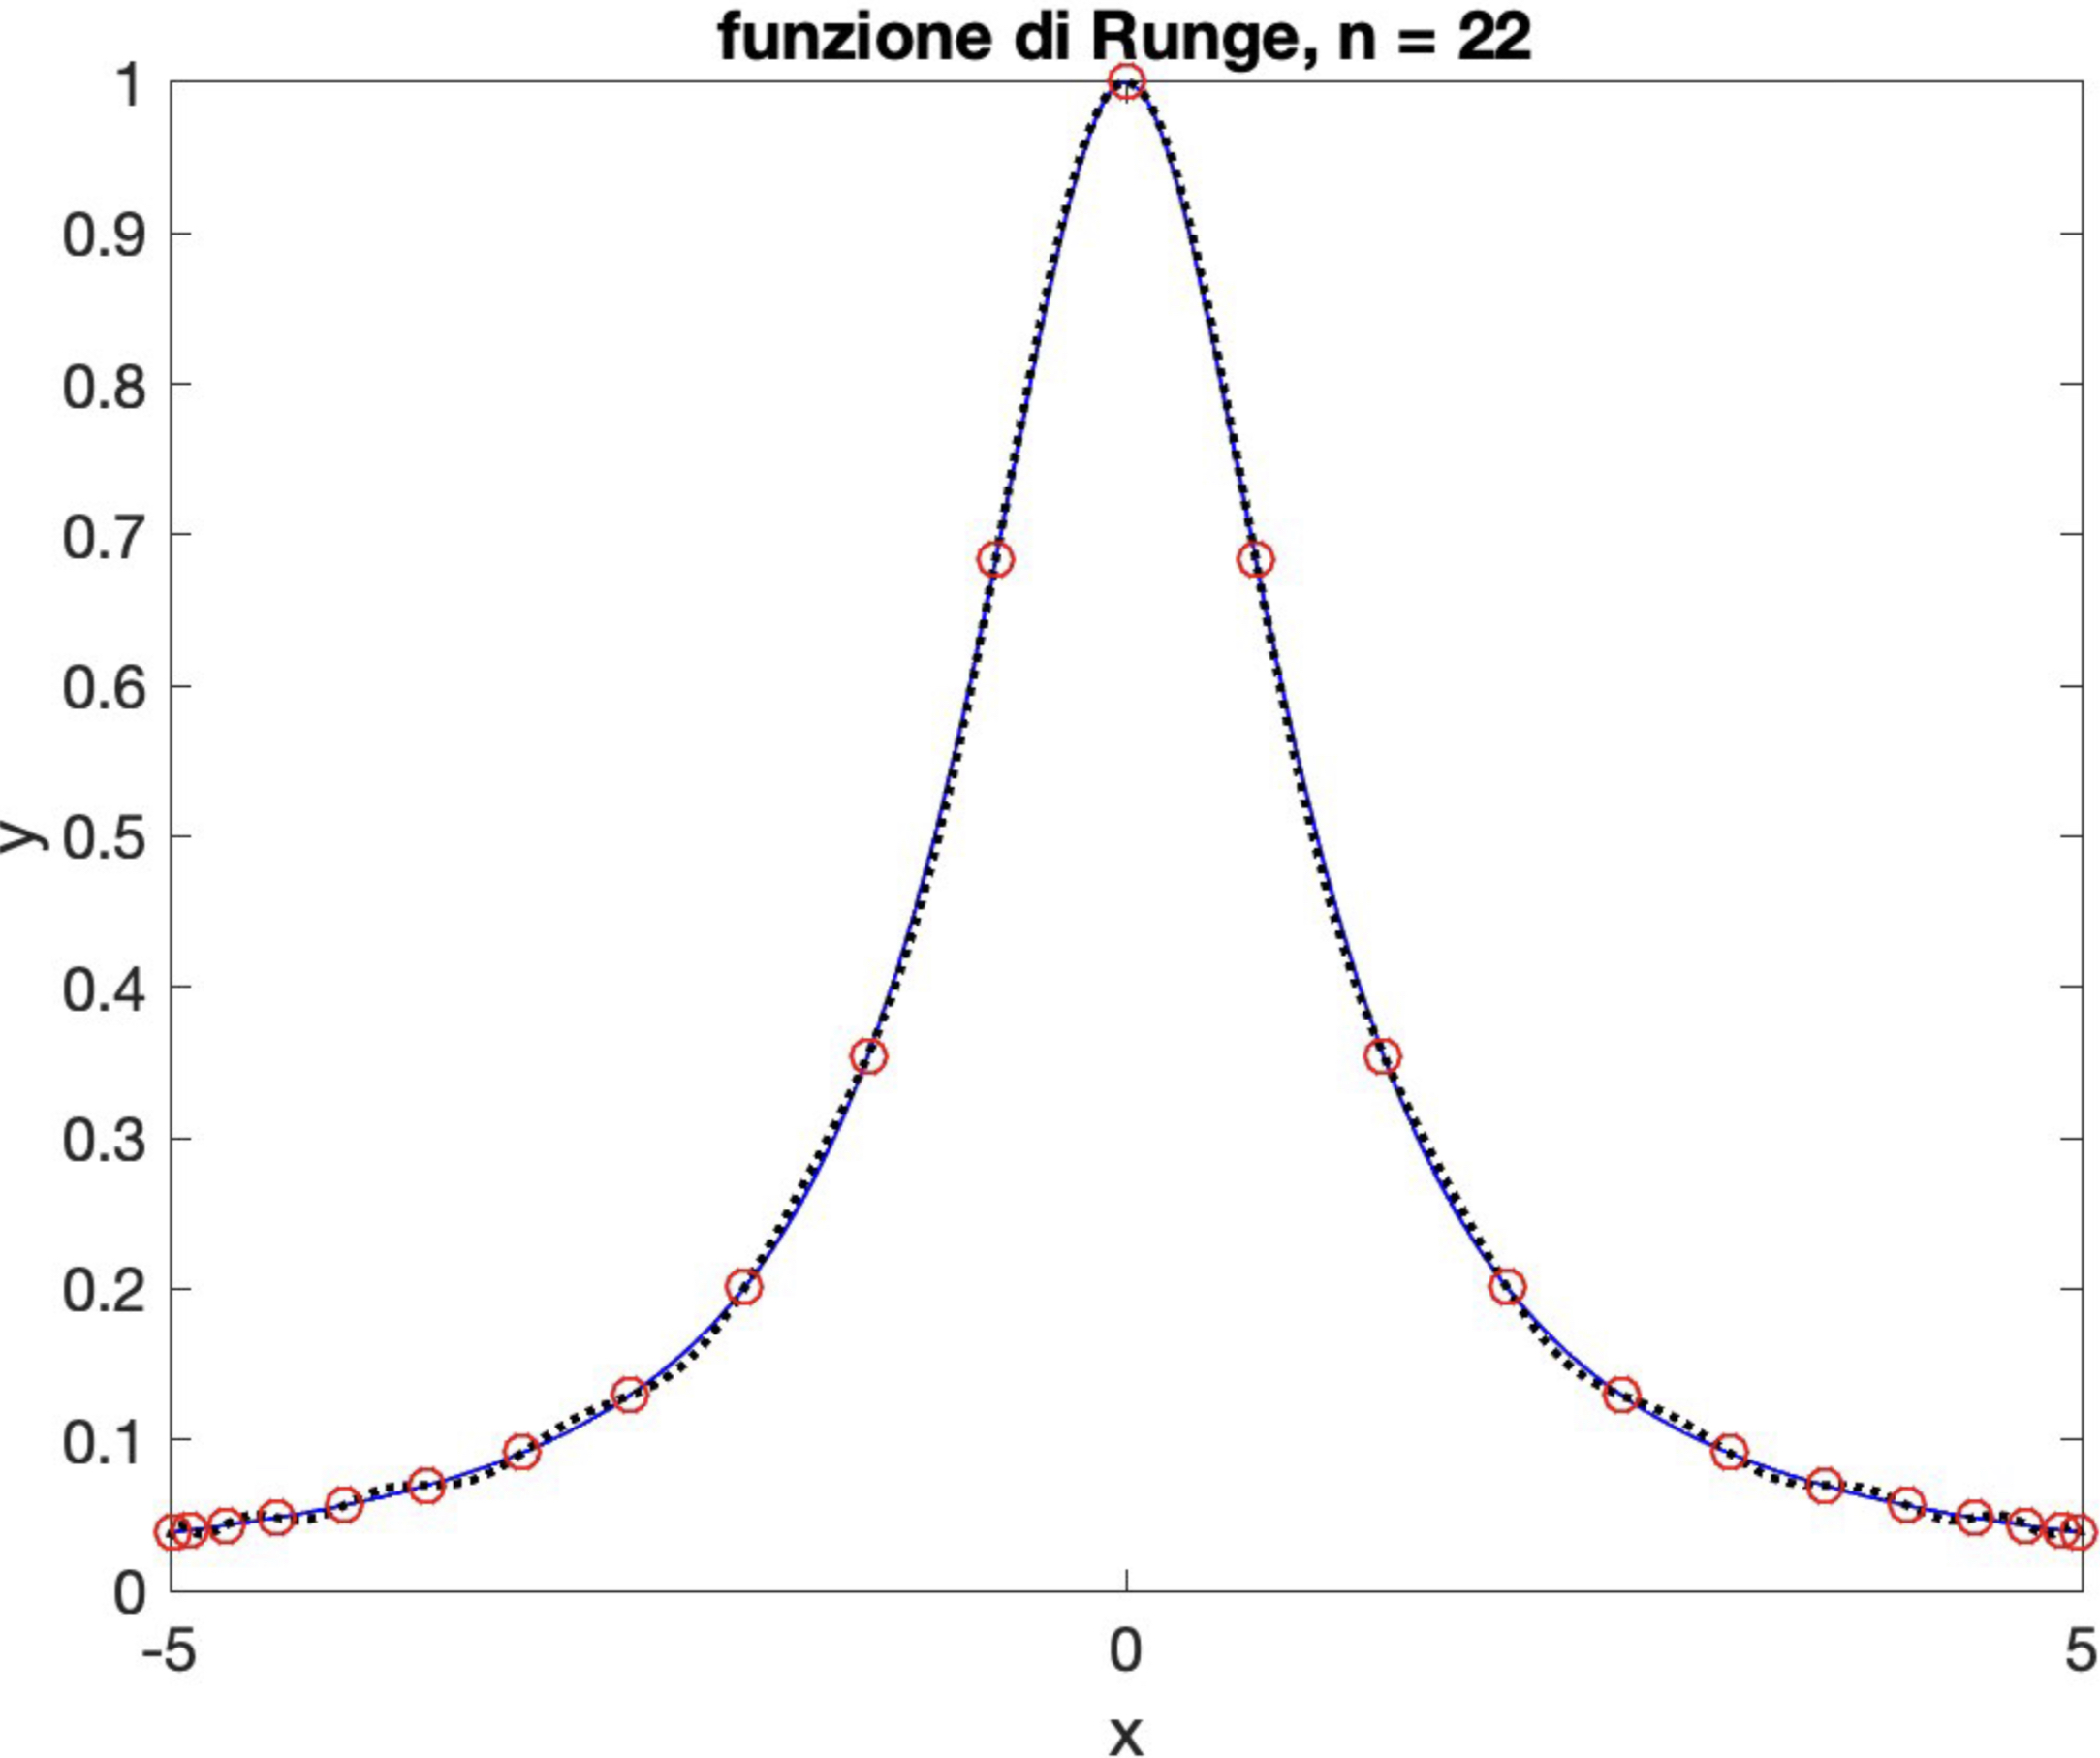
\includegraphics[width=0.5\textwidth]{immagini/fRungeAscChebN=22.jpg}
    \caption{Esempio di crescita di $\Lambda_n$ al crescere di $n$.}\label{fig:fRungeAscChebN=22}
\end{figure}

\subsection{Interpolazione mediante funzioni spline} \footnote{Slide 10-15 PDF 22, Slide 2-3 PDF 23, PG 94 - 100.}
Dalle Figure \ref{fig:fRungeAscChebN=2}-\ref{fig:fRungeAscChebN=22} è possibile ottenere che l'approssimazione migliora all'aumentare del numero di ascisse. Inoltre, è necessario notare che 40 è il numero limite di ascisse per il quale l'approssimazione non migliora, anche se queste sono aumentate. Questo è dovuto al fatto che il numero di condizionamento, pur non essendo particolarmente grande, è influenzato dagli errori di round-off.

In analisi matematica i problemi sono concepiti in aritmetica infinita (ovvero esatta),  ma gli algoritmi sono in aritmetica finita (il problema rappresentato è perturbato, in quanto non è quello reale). Al crescere della grado del polinomio interpolante, le ascisse di Chebyshev evidenziano i limiti dell'utilizzo dell'aritmetica finita, dove il problema è quello di valutare un polinomio di grado elevato in aritmetica finita.

La necessità, quindi, è quella di definire un algoritmo poco sensibile a perturbazioni. Se il numero di ascisse è fatto tendere all'infinito allora l'errore tenderà a 0, ma se è considerato l'errore di round-off accade che gli errori, dovuti all'approssimazione, sono più piccoli degli errori di round-off e sotto questo livello non è possibile scendere. Lo scopo è quello di fornire una soluzione a questo problema tramite ciò che sarà introdotto.

Il punto di partenza per la definizione dell'algoritmo prima citato è il Teorema di Jackson (Teorema \ref{th:Jackson}), il quale lega l'errore di approssimazione al condizionamento del problema tramite la maggiorazione (\ref{eq:maggErrMiglAprrox}). Il problema con la maggiorazione (\ref{eq:maggErrMiglAprrox}) è il seguente: aumentando il grado $n$ del polinomio, il modulo di continuità $\omega$ è reso sempre più piccolo e non è assicurato che non possa essere migliore (così facendo è possibile che venga modificata la decrescenza del modulo di continuità). Tuttavia, se $n$ è piccolo e l'intervallo $[a,b]$ è fissato, $\omega$ non potrà tendere a 0.

In alternativa all'approccio classico è possibile definire quanto segue.

\begin{definition}[Partizione di insieme]
    Dato $[a,b]$ dominio di $f$, una partizione $\Delta$ sull'intervallo $[a,b]$ è definita come
    \begin{equation}\label{eq:defPartizione}
            \Delta = \{\boldsymbol{a}=x_0<x_1<\hdots<x_n=\boldsymbol{b}\},
    \end{equation}
    la quale contiene $n+1$ punti (ovvero ascisse).
\end{definition}

\begin{definition}[Condizione di uniformità della partizione]
    La condizione di uniformità della partizione $\Delta$ (definita come (\ref{eq:defPartizione})) è definita come
    \begin{equation}\label{eq:condUnifPart}
        \boldsymbol h\overset{\footnotemark}{\boldsymbol =}\underset{\boldsymbol{i=1,\hdots,n}}{\boldsymbol\max}\boldsymbol{(x_i-x_{i-1}).}
    \end{equation}
\end{definition}
\footnotetext{Massima ampiezza tra i sottointervalli e la partizione. Ciò che è assunto è: aumentanto il numero dei punti $h\rightarrow 0$, quindi non rimangano zone dell'intervallo $[a,b]$ che, se il numero delle ascisse tende all'infinito, sono senza punti. Se sono aggiunti punti questi sono aggiunti per tutti. Una partizione uniforme garantisce queste proprietà, ovvero (\ref{eq:condUnifPart}).}

È assunto che $h\rightarrow 0,\, n\rightarrow\infty$. Inoltre, è assunto che su ciascun sottointervallo $[x_{i-1}, x_i],\, i=1,\hdots, n$, di $\Delta$ è utilizzato un polinomio di \textbf{grado $\boldsymbol m$ fissato}, interpolante $f(x)$ agli estremi del sottointervallo. Quindi, la nuova funzione interpolante è polinomiale a tratti (ovvero, in ogni sottointervallo è presente un polinomio).
Così facendo, (\ref{eq:maggErrMiglAprrox}) diviene
\begin{equation*}
    \underset{\footnotemark}{||e||}\leq\underbrace{\alpha (1+\Lambda_m)}_{\text{non varia}}\underbrace{\omega\left(f;\frac{h}{m}\right)}_{\text{tende a 0}},
\end{equation*}
dove:
\footnotetext{Se $f$ e $p$ hanno grado $m$, significa che la costante di Lebesque si trasforma in $\Lambda_m$, la quale è fissata, non cambia, ed al posto di $\frac{b-a}{m}$ è inserita la massima ampiezza dell'intervallo.}
\begin{itemize}
    \item $\boldsymbol{m}$ è fissato,
    \item $h\rightarrow 0$, se $\boldsymbol{n}\rightarrow\infty$,
\end{itemize}
con $m$ ed $n$ svincolati.

\footnote{La strategia è dividere il problema in tanti sottoproblemi, ciascuno di essi utilizza un polinomio interpolante di grado fissato $m$ solo agli estremi dell'intervallo.} Date le due precedenti definizioni, il problema del condizionamento diviene meno importante perché $m$ è fissato mentre, se $f\in C^{(0)}$ (vedi (\ref{eq:modCont})), vale il Teorema \ref{th:modContInf}.

Con una lente più formale è possibile definire quanto segue:
\begin{definition}[Spline di $m$ su $\Delta$]\label{def:spline}
    \footnote{Definizione 1 Slide 11 PDF 22, Definizione 4.3 PG 94.}
    $s_m(x)$ è una funzione definita come spline di grado $m$ sulla partizione $\Delta$, la quale è definita come (\ref{eq:defPartizione}), se:
    \begin{enumerate}
        \item $s_m(x)\in C^{(m-1)}[a,b]$; \footnotemark
        \item $s_m|_{[x_{i-1},x_i]}(x)\in\Pi_m,\,\forall i=1,\hdots,n.$
    \end{enumerate}
\end{definition}
\footnotetext{$s_m$ deve essere derivabile $m-1$ volte e le $m-1$ derivate devono essere continue. Se $s_m$ è un polinomio allora soddisferà la condizione perché un polinomio è $C^\infty$ (le derivate successive sono nulle).}

1. e 2. sono condizioni diverse: 1. definisce cos'è una spline di grado $m$ e 2. afferma che la spline coincide con il grado assegnato in ciascun sottointervallo. Una spline interpolante soddisfa le condizioni di interpolazione solite (ovvero $n+1$). È necessario imporre sulla 2. la condizione (\ref{eq:condInterpSpline2}).

\begin{remark}\label{rem:n+mCondIndip}
    \footnote{Slide 12 PDF 22, Teorema 4.11 PG 95.} Denotando con $\boldsymbol{S_m(\Delta)}$ l'insieme delle spline di grado $m$ sulla partizione $\Delta$, contenente $n+1$ ascisse, questo è uno \textbf{spazio vettoriale} di dimensione $\boldsymbol{m+n}$.
\end{remark}

La dimensione di uno spazio vettoriale è importante per individuare una spline univocamente. Un risultato importante dell'Osservazione \ref{rem:n+mCondIndip} è il seguente: è possibile individuare in modo univoco una spline di grado $m$ sulla partizione $\Delta$, con $m+n$ condizioni distinte, quindi indipendenti. Inoltre, la dimensione di uno spazio vettoriale è utilizzata per determinare quante condizioni sono necessarie per individuare un oggetto.

\begin{remark}
    \footnote{Slide 12 PDF 22.} $\Pi_m\subset S_m(\Delta).$
\end{remark}

Dalla precedente osservazione è possibile dedurre che lo spazio vettoriale dei polinomi di grado al più $m$ è contenuto nell'insime delle spline di grado $m$. Inoltre, è necessario ricordare che il polinomio di grado $m$ è una funzione $C^\infty$ e, rispetto a ciascun sottointervallo, coincide con se stesso.

\begin{definition}\label{def:interpFInDelta}
    \footnote{Definizione 2 Slide 12 PDF 22, Definizione 4.4 PG 95. Ciò che è tra parentesi è un aggiunta maggiore chiarezza. Date le condizioni 1. e 2. della Definizione \ref{def:spline} è possibile dare la seguente definizione.}
    Una spline $s_m(x)$ sulla partizione $\Delta$ interpola una funzione $f(x)$ (nei nodi della partizione) se (valgono le seguenti condizioni di interpolazione): 
    \begin{equation}\label{eq:condInterpSpline}
        \boldsymbol{s_m(x_i)=f(x_i)\equiv f_i,\quad i=0,\hdots,n.}
    \end{equation}
\end{definition}

La definizione aggiunge alle due condizione necessarie affinché $s_m(x)$ sia definita spline, le condizioni necessarie affinché $s_m(x)$ interpoli $f(x)$.

\begin{remark}
    \footnote{Slide 13 PDF 22, PG 95.} Le sole condizioni di interpolazione ($n+1$) permettono di individuare univocamente le spline di grado 1, anche dette spline lineari. In questo caso una spline lineare è la spezzata che congiunge i punti di interpolazione $(x_i,f_i),$ per $i=0,\hdots, n$. La spline lineare interpolante è data da 
    \begin{equation}\label{eq:splineLineare}
        \boldsymbol{s_1|_{[x_{i-1}, x_i]}(x)=\frac{(x-x_{i-1})f_i+(x_i-x)f_{i-1}}{x_i-x_{i-1}},\quad i=1,\hdots,n.}
    \end{equation}
\end{remark}

\begin{figure}
    \centering
    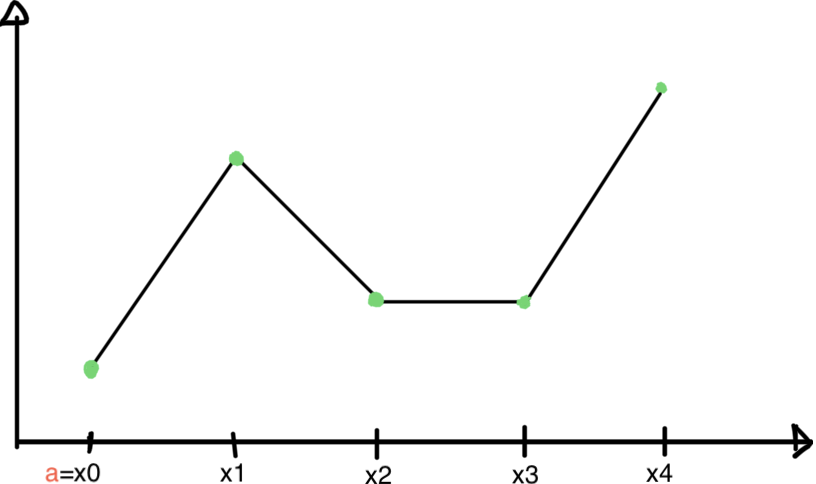
\includegraphics[width=0.5\textwidth]{immagini/s_mN=4.png}
    \caption{Esempio di spline con $n=4$.}\label{fig:s_mN=4}
\end{figure}

Quindi $s_1(x)$ è il segmento che congiunge i punti in coordinate $(x_{i-1},f_{i-1})$ e $(x_i,f_i)$. Questo sarà utile quando saranno calcolate spline diverse dalle lineari.

La definizione di spline di grado $m$ (Definizione \ref{def:spline}) prescinde dal fatto che la spline sia interpolante la funzione. All'interno dello spazio vettoriale l'obbiettivo è quello di individuare una spline interpolante, possibilmente unica.
Quando il grado della spline aumenta allora esistono diverse spline di grado superiore, per le quali ciascuna sarà una spline di grado $m$ interpolante. Queste spline differendo per poco, dato che le condizioni mancanti saranno imposte e ciascuna scelta riguardo le condizioni imposte genera spline diverse.

La condizione 1. della Definizione \ref{def:spline} implica che la spline $s_m$ debba essere una funzione di classe $C^{(m-1)}[a,b]$. Questo requisito richiede di imporre delle condizioni sui punti interni della partizione $x_1,\hdots,x_{n-1}$, ovvero i punti di contiguità tra i sottointervalli $[x_{i-1},x_i]$ e $[x_i,x_{i+1}],$ per $ i=1,\hdots,n-1$. Ovvero, le condizioni da imporre sono le seguenti:
\begin{equation}\label{eq:condInterpSpline2}
    \begin{matrix}
        s_m^{(\boldsymbol{j})}|_{[x_{i-1},\boldsymbol{x_i}]}(\boldsymbol{x_i})= s_m^{(\boldsymbol{j})}|_{[\boldsymbol{x_i},x_{i+1}]}(\boldsymbol{x_i}),\\
        j=0,\hdots,m-1,\; i=1,,\hdots,n-1.
    \end{matrix}
\end{equation}

\noindent\footnotemark In altri termini, i due polinomi devono raccordarsi fino alla derivata $m-1$ nel punto $x_i$. Quando $j=0$ è richiesta solo la continuità, se è ricercata una spline interpolante in quei punti "viene gratis". Entrambi i polinomi devono assumere il valore della funzione che sta essendo interpolata. Il problema sono le derivate successive.
\footnotetext{Significa che sono presenti due sottointervalli contigui: a sinistra del primo sottointervallo la spline coincide con un polinomio, nel secondo sottointervallo con un altro polinomio di grado $n$. La $j$ rappresenta la derivata $j$-esima di $s_m$ e $x_i$ il punto continguo degli insiemi.}

Vale il seguente risultato.

\begin{theorem}\label{th:gradoDervSpline}
    \footnote{Slide 14 PDF 22, Teorema 4.10 PG 95} Se $s_m$ è una spline di grado $m\geq 2$ sulla partizione $\Delta$, allora $s'_m(x)$ è una spline di grado $m-1$ sulla stessa partizione.
\end{theorem}
\begin{proof}
    Se $s_m(x)$ è una spline di grado $m\geq 2$ sulla partizione $\Delta$, allora:
    \begin{enumerate}
        \item $s_m(x)\in C^{(m-1)}[a,b]\overset{\footnotemark}{\Rightarrow} s'_m(x)\in C^{(m-2)}[a,b];$
        \footnotetext{Data una funzione di una qualsiasi classe $m$ allora la sua derivata è di $m-1$. È eliminata un'equazione ma le successive derivate rimangono.}
        \item $s_m|_{[x_{i-1},x_i]}(x)\in\Pi_m,\,\forall i=1,\hdots,n\Rightarrow s'_m|_{[x_{i-1},x_i]}(x)\in\Pi_{m-1},\;\forall i=1,\hdots,n.$
    \end{enumerate}
    Pertanto, $s'_m\in S_{m-1}(\Delta).$
\end{proof}
Dato che $m\geq 2\,(>0)$, per il Teorema, quindi la funzione è continua (questo vale anche per le funzioni lineari). ($C^{-1}$ significa che la funzione è costante.)

\subsection{Spline cubiche}
\begin{remark}
    \footnote{Slide 15 PDF 22.}
    Nella pratica computazionale assumono particolare importanza le \textbf{spline cubiche ($\boldsymbol{m=3}$)}. Se è ricercata la spline cubica interpolante sono necessarie due ulteriori condizioni, ognuna delle quali darà origine ad una spline cubica interpolante generalmente diversa, oltre alle condizioni definite in (\ref{eq:condInterpSpline}). Una funzione di grado 3 sarà interpolata da un polinomio di grado 3 e può accadere che più spline coincidano.
\end{remark}

I motivi per i quali è scelta la spline cubica sono le condizioni solitamente asimmetriche rispetto agli estremi dell'intervallo. La derivata prima di una spline quadratica è continua, ha un profilo smooth e per questo sono scelte per l'approssimazione di funzioni. Sono utilizzate le spline cubiciche e non quadratiche dato che l'unica condizione è la non simmetria.

Per individuare univocamente una spline cubica definita sulla partizione $\Delta$, occorrono $n+3$ ($m=3$) condizioni indipendenti tra loro. Se è ricercata una spline interpolante una data funzione $f(x)$, le condizioni di interpolazione (\ref{eq:condInterpSpline}) forniscono $n+1$ condizioni. Pertanto, rimangono da fissare \textbf{2 condizioni addizionali} per determinare univocamente una spline cubica, dove ciascuna coppia di condizioni addizionali darà origine ad una spline interpolante, le quali sono \textbf{generalmente diverse tra loro.} Le condizioni di interpolazione sono importanti ed esiste un certo numero di modi per imporle, ciascuno di questi modi genererà una spline interpolante, generalmente le spline generate sono diverse.

Sono esaminante \textbf{4 possibili implementazioni} delle condizioni aggiuntive e neccessarie da imporre per determinare una spline cubica interpolante.
\subsubsection{Spline cubica naturale}
\footnote{Slide 4 PDF 23, PG 96.} 
Questa spline è determinata dalle due seguenti condizioni:
\begin{equation}\label{eq:condSplineCubNat}
    \boxed{s''_3(a)=0,\quad s''_3(b)=0.}
\end{equation}

La spline cubica naturale è quella che minimizza la curvatura totale della curva (non sarà trattato). Questa spline è scelta perché porta all'algoritmo di misurazione più efficiente tra tutti (non sarà trattato).

\subsubsection{Spline cubica completa}\footnote{Nota precedente.}
Questa spline è determinata dalle due seguenti condizioni:
\begin{equation}\label{eq:condSplineCubComp}
    \boxed{s'_3(a)=f'(a),\quad s'_3(b)=f'(b)}
\end{equation}

Negli estremi della partizione $\Delta$ è imposta una condizione di interpolazione di Hermite.
Dal punto di vista computazionale è implementata con variazioni della spline cubica naturale.

\subsubsection{Spline cubica interpolante periodica} \footnote{Nota precedente. Questa non è applicata ad una funzione interpolanda ma a funzioni periodiche.}
Questo tipo di spline è utilizzata supponendo che la funzione $f(x)$ sia una funzione periodica sull'intervallo $[a,b]$. Infatti vale la segeunte osservazione:

\begin{remark}
    Quanto scritto significa che $b-a$, che è l'ampiezza dell'intervallo, deve essere un multiplo intero del periodo $T$ della funzione [\footnote{È possibile un'efficienza maggiore esprimendo $b$ come $b=T\cdot a$.}].
\end{remark}

\begin{example}
    Se $f(x)=\sin(x)\Rightarrow b$ deve essere un multiplo di $2\pi$, altrimenti la funzione non è periodica (ad esempio con $[0,\pi]$).
\end{example}

Dalle condizioni di interpolazioni e per la periodicità di $f(x)$, è noto quanto segue:
\begin{equation*}
    s_3(a)=f(a)=f(b)=s_3(b).
\end{equation*}

Se $\boldsymbol{f(x)\in C^{(2)}[a,b]}$, ovvero $f$ è più che continua, \textbf{come funzione periodica}, allora:

\begin{equation}\label{eq:condPeriod}
    f'(a)=f'(b),\quad f''(a)=f''(b).
\end{equation}

Dato che è richiesto che la spline cubica $s_3\in C^{(2)}[a,b]$, per la definizione di spline (Definizione \ref{def:spline}), è imposto che lo sia anche come funzione periodica. Analogamente a (\ref{eq:condPeriod}), sono imposte le seguenti condizioni aggiuntive:

\begin{equation}\label{eq:condSplineCubPer}
    \boxed{s'_3(a)=s'_3(b),\quad s''_3(a)=s''_3(b).}
\end{equation}

\begin{remark}
    Questo tipo di spline è applicato esclusivamente al caso di funzioni periodiche sull'intervallo $[a,b]$.
\end{remark}

\paragraph{Intermezzo:}È possibile costruire spline cubiche interpolanti una funzione periodica  del tipo natuale, periodica e completa ottenendo risultati generalmente diversi fra loro.

\subsubsection{Spline cubica interpolante not-a-knot}
\begin{remark}\footnote{Slide 5 PDF 23, PG 97}
    Questa spline è implementata nella \textit{function \textbf{spline}} di Matlab.
\end{remark}

\textbf{Questa spline non necessita di ulteriori informazioni oltre a quelle di interpolazione}, le condizioni aggiuntive sono  imposte in modo implicito. 

È noto che nei primi due sottointervalli siano presenti due polinomi di grado 3 (e così anche negli ultimi due). Ciò che è richiesto è che i due polinomi ed i primi due sottoinsiemi, tramite l'unione ($[x_0,x_1]\cup[x_1,x_2]=[x_0,x_1]$), coincidano. In questo modo è imposta una condizione in meno in modo esplicito. 

La spline not-a-knot fa in modo che il nodo 1 ($x_1$) non sia il nodo che definisce una spline in senso classico. Questo è dovuto al fatto che è presente un unico polinomio nel primo e secondo sottoinsieme, in genere sono distinti. La stessa cosa avviene anche negli ultimi due sottointervalli.

Le condizioni aggiuntive sono imposte in modo implicito come segue:
\begin{enumerate}
    \item lo \textbf{stesso polinomio cubico definisce} la spline $\boldsymbol{s_3}$ \textbf{sui primi 2 sottointervalli} $\boldsymbol{[x_0,x_1]}$ e $\boldsymbol{[x_1,x_2]}$;
    \item \footnotemark \textbf{simmetricamente}, \textbf{lo stesso polinomio cubico} definisce la spline $s_3$ sugli ultimi due sottointervalli $[x_{n-2},x_{n-1}]$ e $[x_{n-1},x_n]$.
    \footnotetext{La condizione di simmetria è importante perché, data la funzione $f(x)$, è definita $g(x)$ come $f$ rovesciando la direzione di $x$. $g(a)=f(b)$ se $f(x)$ e $g(x)$ hanno lo stesso verso. Le due funzioni hanno lo stesso grafico ed è importante che abbiano la stessa approssimazione. Sotto le stesse condizioni è ottenuto lo stesso risultato.}
\end{enumerate}

Imporre questa condizione per la 1. significa quanto segue (similmente per 2.):
\begin{equation*}
    p_1(x)=s_3|_{[x_0,x_1]}(x),\quad p_2(x)=s_3|_{[x_1,x_2]}(x),
\end{equation*}
dove è ricercato $p_1(x)=p_2(x)\in\overset{\footnotemark}{\Pi_3}$. In $x_1$, tramite le condizioni di interpolazione, è ottenuto $p_1(x_1)=p_2(x_1)$. Il raccordo deve valere anche per le derivate prima e seconda, ovvero:
\begin{equation*}
    p'_1(x_1)=p'_2(x_1)\quad\land\quad p''_1(x_1)=p''_2(x_1).
\end{equation*}
\footnotetext{Un polinomio di grado 3 ha 4 coefficienti, 4 gradi libertà e $\Pi_3$ è uno spazio vettoriale di dimensione 4.}

Se è imposto che $\overset{\footnotemark}{p'''_1(x_1)}\overset{\footnotemark}{=}\overset{\footnotemark}{p'''_2(x_1)}$ allora $p_1(x)=s_3(x)=p_2(x),\, x\in [x_0,x_2]$. Quindi, definita la spline $s_3(x)$ e le sue derivate come 
\begin{equation*}
    \begin{matrix}
        s_3|_{[x_0,x_2]}(x)\in\Pi_3,\\
        s'_3|_{[x_0,x_2]}(x)\in\Pi_2,\\
        s''_3|_{[x_0,x_2]}(x)\in\Pi_1,\\
        \underset{\footnotemark}{s'''_3|_{[x_0,x_2]}(x)}\in\Pi_0,
    \end{matrix}
\end{equation*}
è possibile imporre condizione sui primi due sottintervalli della partizione $\Delta$, la quale è
\begin{equation*}
    \boxed{\frac{s''_3(\boldsymbol{x_1})-s''_3(x_0)}{x_1-x_0}=\frac{s''_3(x_2)-s''_3(\boldsymbol{x_1})}{x_2-x_1}.}
\end{equation*}

\addtocounter{footnote}{-3}
\footnotetext{Restrizione sul primo sottointervallo.}

\stepcounter{footnote}
\footnotetext{È presente un raccordo $C^{(2)}$ nel punto di continuità ed è noto il raccordo della derivata terza. Inoltre, la funzione ha derivate che coincidono in più punti, quando due polinomi sono lo stesso, per $x\in [x_0,x_1]\cup[x_1,x_2]=[x_0,x_2]$. Le precedenti sono 4 condizioni distinte con 4 gradi di libertà.}

\stepcounter{footnote}
\footnotetext{Restrizione sul secondo sottointervallo.}

\stepcounter{footnote}
\footnotetext{Questo polinomio di grado 0 è una costante, il coeffciente lineare della retta derivata seconda, ed è la stessa a sinistra ed a destra di $x_1$. Questo significa che il rapporto incrementale della derivata seconda su $x_0,\, x_1$ e $x_2$  deve essere lo stesso.}

Simmetricamente, sugli ultimi due sottointervalli, sarà imposto:
\begin{equation*}
    \boxed{\frac{s''_3(x_n)-s''_3(\boldsymbol{x_{n-1}})}{x_n-x_{n-1}}=\frac{s''_3(\boldsymbol{x_{n-1}})-s''_3(x_{n-2})}{x_2-x_1}.}
\end{equation*}

$\boldsymbol{x_1}$ e $\boldsymbol{x_{n-1}}$ precedenti non sono considerati nodi della partizione in quanto sono imposte le condizioni di interpolazione e le condizioni di default.

Ciò che è stato appena definito nei riquadri è una conveniente espressione, in virtù del Teorema \ref{th:gradoDervSpline}, delle condizioni aggiuntive della spline cubica not-a-knot, ovvero:
\begin{equation}\label{eq:condSplineCubNotAKnot}
    s'''_3|_{[x_0,x_1]}(x_1)=s'''_3|_{[x_1,x_2]}(x_1),\quad s'''_3|_{[x_{n-2},x_{n-1}]}(x_{n-1})=s'''_3|_{[x_{n-1},x_n]}(x_{n-1}).
\end{equation}

La rappresentazione delle condizioni (\ref{eq:condSplineCubNotAKnot}) tramite le derivate seconde è utile al fine di definire l'unicità della spline interpolante. Dal punto di vista computazionale è importante che le condizioni siano imposte sulla derivata seconda.

\begin{remark}
    \footnote{Slide 2 PDF 24, Osservazione 4.5 PG 97.} L'ampiezza dell'intervallo $i$-esimo della partizione $\Delta$, definita come (\ref{eq:defPartizione}), è definita come
    \begin{equation}\label{eq:defAmpiezzaInt}
        \boldsymbol{h_i=x_i-x_{i-1},\quad i=1,\hdots,n},
    \end{equation}
    dove la massima ampiezza definita come 
    \begin{equation*}
        \boldsymbol{h=\underset{i=1,\hdots,n}{max}h_i},
    \end{equation*}
    allora è possibile dimostrare, se $f\in C^{(4)}[a,b]$, che per tutte le spline cubiche esaminate vale
    \begin{equation*}
        \left|\left|f^{(i)}-s^{(i)}_3\right|\right|=O\left(h^{4-i}\right),\quad i=0,1,2.
    \end{equation*}
\end{remark}

Quanto osservato significa che le spline cubiche consentono di approssimare efficientemente funzioni regolari, senza preoccuparsi troppo della scelta della partizione (ad esempio quella uniforme è sufficiente).

Approssimare la funzione significa approssimare uniformemente anche la derivata prima e seconda. Questo risultato è esatto per tutte le spline cubiche tranne per la naturale, dove, se forzata, la derivata seconda negli estremi è 0. Questo non è sempre vero in quanto è possibile introdurre errori sistematici. È possibile affermare che l'errore diminuisce rapidamente quando è ottenuto dagli estremi dell'intervallo.

\subsection{Calcolo (pratico) di una spline cubica}\label{ssec:calcSplineCub}\footnote{Slide 2-13 PDF 24, PG 97-101.}
Per trattare questa Sezione è utile la Sezione \ref{ssec:risSistTridiag}.

Il problema da affrontare è quello del calcolo della spline cubica $s_3(x)$ interpolante $f(x)$ sulla partizione, definita come in (\ref{eq:defPartizione}), $\Delta=\{a=x_0<x_1<\hdots<x_n=b\}$.

Per determinare un algoritmo efficiente per il calcolo di una spline cubica, oltre a (\ref{eq:defAmpiezzaInt}), sarà usata la notazione seguente:
\begin{equation}\label{eq:s''3(xi)}
    \boldsymbol{m_i=s''_3(x_i),\quad i=0,\hdots,n.}
\end{equation}

In particolare saranno esaminati gli algoritmi per il calcolo delle spline cubiche naturali e not-a-knot. Sarà altresì trattato come, utilizzando questi argomenti, con piccoli cambiamenti, possono essere ottenute le spline naturali e complete. È necessario individuare quali siano le condizioni, in termini di $m_i$ definiti tramite (\ref{eq:s''3(xi)}), che caratterizzano l'un l'altra.

Il calcolo della spline cubica naturale è semplice ed, inoltre, è stato trattato come le condizioni imposte riguardino l'annullamento della derivata seconda, negli estremi $a$ e $b$. L'annullamento della derivata seconda e la notazione (\ref{eq:s''3(xi)}) implicano che, per una \textbf{spline cubica naturale}, le condizioni diventino
\begin{equation}\label{eq:condSplineNat}
    \boldsymbol{m_0=0=m_n}.
\end{equation}

Imponendo (\ref{eq:defAmpiezzaInt}), \textbf{le condizioni aggiuntive della spline not-a-knot}, ovvero degli estremi sinistro e destro (\ref{eq:condSplineCubNotAKnot}), diventano
\begin{equation*}
    \frac{m_1-m_0}{h_1}=\frac{m_2-m_1}{h_2},\quad \frac{m_{n-1}-m_{n-2}}{h_{n-1}}=\frac{m_n-m_{n-1}}{h_n}
\end{equation*}
ovvero $h_2(m_1-m_0)=h_1(m_2-m_1),\, h_{n}(m_{n-1}-m_{n-2})=h_{n-1}(m_{n}-m_{n-1})$, dalle quali sono ottenute le condizioni
\begin{equation}\label{eq:condSplineCubNotAKnot2}
    \boldsymbol{h_2m_0-(h_1+h_2)m_1+h_1m_2=0}\quad\boldsymbol{h_{n-1}m_n-(h_{n-1}+h_n)m_{n-1}+h_nm_{n-2}=0}.
\end{equation}

\textbf{(\ref{eq:condSplineCubNotAKnot2}) sono le condizioni aggiuntive per le spline not-a-knot}.

Riguardo le altre condizioni $\{m_i\}$, è possibile osservare che, se $s_3(x)$ è una spline cubica sulla partizione $\Delta$, allora $s'_3(x)$ è una spline di grado 2 sulla stessa partizione, e $s''_3(x)$ è una spline lineare su $\Delta$. Pertanto, essendo $s''(x)$ una spline lineare, da (\ref{eq:splineLineare}) e (\ref{eq:s''3(xi)}), è ottenuto che
\begin{equation*}
    s''_3(x)\underset{\footnotemark}{=}\frac{(x-x_{i-1})m_i+(x_i-x)m_{i-1}}{\equalto{h_i}{x_i-x_{i-1}}},\quad\boldsymbol{x\in[x_{i-1}, x_i]},\; i=1,\hdots,n.
\end{equation*}\footnotetext{Le $m_i$ non sono note. Sono noti i valori della derivata seconda della spline che assume nelle asisse di interpolazione. Quindi la derivata seconda della spline è la spline lineare che interpola gli $m_i$.}

Integrando membro a membro la precedente equazione è ottenuto
\begin{equation}\label{eq:s'_3(x)}
    s'_3(x)=\frac{(x-x_{i-1})^2m_i-(x_i-x)^2m_{i-1}}{2h_i}+\underset{\footnotemark}{q_i},\quad x\in [x_{i-1}, x_i],\; i=1,\hdots,n.
\end{equation}\footnotetext{Costante d'integrazione.}

\noindent\footnote{Non conoscendo le $m_i$ non è possibile calcolare la derivata seconda. Integrando membro a membro sarà ottenuta la derivata prima della spline e questa sarà la restrizine all'$i$-esimo sottointervallo $[x_{i-1},x_i]$.}
Integrando nuovamente è ottenuta un'ulteriore spline:

\begin{equation}\label{eq:s3Ign}
    s_3(x)=\frac{(x-x_{i-1})^3\boldsymbol{m_i}+(x_i-x)^3\boldsymbol{m_{i-1}}}{6h_i}+\boldsymbol{q_i}(x-x_{i-1})+\underset{\footnotemark}{\boldsymbol{r_i}},\quad x\in[x_{i-1},x_i],\; i=1,\hdots,n.
\end{equation}\footnotetext{Nuova costante di integrazione.}

\noindent\footnote{Fossero noti gli $m_i$ e fosse possibile determinare le costanti di integrazione $r_i$ e $q_i$, allora sarebbe possibile calcolare il polinomio di grado 3, il quale costituisce la restrizione della spline nell'intervallo d'interesse. Ciò che sarà richiesto nell'elaborato, quando sarà necessario calcolare la spline nei punti assegnati, sarà calcolare la spline nei punti interpolanti. Adesso saranno eliminate le costanti $q_i$ e $r_i$ imponendo condizione di interpolazione agli estremi di ciascun sottointervallo.}
Imponendo le condizioni di interpolazione a ciascun intervallo, è ottenuto quanto segue:
\begin{itemize}
    \item $s_3(x_1)=\frac{h_i^2}{6}m_{i-1}+r_i=f(x_{i-1})$, dalla quale è ottenuta \begin{equation}\label{eq:ri}
        \underset{\footnotemark}{\boldsymbol{r_i}}\boldsymbol{=f(x_{i-1})-\frac{h_i^2}{6}m_{i-1}},
    \end{equation}
    dove $f(x_{i-1})$ ed $h_i^2$ sono valori noti.
    \item $s_3(x_i)=\frac{h_i^2}{6}m_i+q_ih_i+r_i\overset{\footnotemark}{=}f(x_i)$. Pertanto,
    \begin{equation*}
        \begin{matrix}
             h_iq_i &=& f(x_i)-r_i-\frac{h_i^2}{6}m_i &\overset{\footnotemark}{=}& f(x_i)-f(x_{i-1})+\frac{h_i^2}{6}(m_{i-1}-m_i) &\Rightarrow&\\
            &\Rightarrow& q_i &=& \frac{f(x_i)-f(x_{i-1})}{\underbrace{x_i-x_{i-1}}_{h_i}}+\frac{h_i}{6}(m_{i-1}-m_i).&&
        \end{matrix}
    \end{equation*}
    Da cui,
    \begin{equation}\label{eq:qi}
        \boldsymbol{q_i=f[x_{i-1},x_i]+\frac{h_i}{6}(m_{i-1}-m_i).}
    \end{equation}
\end{itemize}
\addtocounter{footnote}{-2}
\footnotetext{Non calcolabile perché le $m_i$ non sono note.}

\stepcounter{footnote}
\footnotetext{Con questa uguaglianza sono ricavate le $g_i$ perché le $r_i$ sono state calcolate.}

\stepcounter{footnote}
\footnotetext{Sostituzione di $r_i$ con (\ref{eq:ri}).}

Ora è necessario calcolare gli $\{m_i\}$, per poter calcolare le costanti $q_i$ e $r_i$ di ciascun sottointervallo $[x_{i-1},x_i]$ e quindi (\ref{eq:s3Ign}).

Imponendo che $s'_3(x)$ sia continua nei punti $x_i,\; i=1,\hdots,n$, ovvero imponendo che
\begin{equation*}
    s'_3|_{[x_{i-1}, x_i]}(x_i)=s'_3|_{[x_i, x_{i+1}]}(x_i),
\end{equation*}
è ottenuto, da (\ref{eq:s'_3(x)}):
\begin{equation*}
    \frac{h_i}{2}m_i+q_i=-\frac{h_{i+1}}{2}m_i+q_{i+1},\quad i=1,\hdots,n-1.
\end{equation*}

Quindi [\footnotemark]:
\begin{equation*}
    3h_im_i+h_i(m_{i-1}-m_i)+3h_{i+1}m_i-h_{i+1}(m_i-m_{i+1})=6\left(f[x_i,x_{i+1}]-f[x_{i-1},x_i]\right),\quad i=1,\hdots,n-1.
\end{equation*}
\footnotetext{Moltiplicando per 6 e portando a sinistra dell'uguale tutto ciò che dipende da $m$, è ottenuto quanto segue.}
Raggruppando gli $m_i$ con gli stessi indici a primo membro è ottenuto quanto segue:
\begin{equation*}
    h_im_{i-1}+2(h_i+h_{i+1})m_i+h_{i+1}m_{i+1}=6(f[x_i,x_{i+1}]-f[x_{i-1},x_i]),\quad i=1,\hdots,n-1.
\end{equation*}
Dividendo membro a membro per $h_i+h_{i+1}=x_{i+1}-x_{i-1},$ è ottenuto:
\begin{equation}\label{eq:eqCalcMi}
    \begin{matrix}
        \equaltoup{\boxed{\frac{h_i}{h_i+h_{i+1}}}}{\varphi_i}\,m_{i-1}+2m_i+\equaltoup{\boxed{\frac{h_{i+1}}{h_i+h_{i+1}}}}{\xi_i}\,m_{i+1}&=&6\,\frac{f[x_i,x_{i+1}]-f[x_{i-1},x_i]}{x_{i+1}-x_{i-1}}&\overset{\footnotemark}{=}&6\,f[x_{i-1},x_i,x_{i+1}],\\
        && && i=1,\hdots,n-1.
    \end{matrix}
\end{equation}\footnotetext{Per (\ref{eq:P5DiffDiv}).} 

\begin{remark}\label{re:varphi+xi=1}\footnote{Slide 9 PDF 24.}
    $\boldsymbol{\varphi_i,\, \xi_i>0,\, \varphi_i+\xi_i=1.}$
\end{remark}

Le equazioni (\ref{eq:eqCalcMi}) sono un sistema di $n-1$ equazioni nelle $n+1$ incognite $\{m_0,\hdots,m_n\}$.

\textbf{Nel caso} di \textbf{spline naturali}, tenendo di conto delle condizioni (\ref{eq:condSplineNat}), è \textbf{ottenuto il sistema tridiagonale} 
\begin{equation*}
    \begin{pmatrix}
        2 & \xi_1 & && \\
        \varphi_2 & 2 & \xi_2&&\\
        &\ddots & \ddots &\ddots&\\
        &&\ddots & \ddots &\xi_{n-2}\\
        &&&\varphi_{n-1} & 2
    \end{pmatrix}\begin{pmatrix}
        m_1\\
        m_2\\
        \vdots\\
        \vdots\\
        m_{n-1}
    \end{pmatrix}=6\begin{pmatrix}
        f[x_0,x_1,x_2]\\
        f[x_1,x_2,x_3]\\
        \vdots\\
        \vdots\\
        f[x_{n-2},x_{n-1},x_n]
    \end{pmatrix}.
\end{equation*}

Dall'Osservazione \ref{re:varphi+xi=1} è possibile notare che la matrice dei coefficienti è diagonale dominante sia per righe che per colonne e quindi la sua fattorizzazione $LU$ è definita\textbf{. Calcolati i valori} $\boldsymbol{\{m_i\}}$ \textbf{incogniti, la spline naturale è calcolata sostituendoli, assieme a (\ref{eq:ri})-(\ref{eq:qi}), in (\ref{eq:s3Ign}).}

Ragionamento analogo vale \textbf{per la spline cubica not-a-knot} ottenenuta imponendo le relative condizioni aggiuntive, per la quale \textbf{le condizioni (\ref{eq:condSplineCubNotAKnot2}) e (\ref{eq:eqCalcMi}) danno origine al sistema lineare}
\begin{equation}\label{eq:sisTridSpline}
    \begin{pmatrix}
        \xi_1 & -1 & \varphi_1 && \\
        \varphi_1 & 2 & \xi_1&&\\
        &\ddots & \ddots &\ddots&\\
        &&\varphi_{n-1}& 2 &\xi_{n-1}\\
        && \xi_{n-1} & -1 & \varphi_{n-1}
    \end{pmatrix}\begin{pmatrix}
        m_0\\
        m_1\\
        \vdots\\
        m_{n}
    \end{pmatrix}=6\begin{pmatrix}
        0\\
        f[x_0,x_1,x_2]\\
        \vdots\\
        f[x_{n-2},x_{n-1},x_n]\\
        0
    \end{pmatrix}.
\end{equation}

Sostituendo alla prima equazione la somma delle prime due, all'ultima la somma delle ultime due e moltiplicando a destra la matrice dei coefficienti per
\begin{equation*}
    \begin{pmatrix}
        1 & -1 & -1&&\\
        & 1 &&&\\
        &&\ddots&&\\
        &&&1&\\
        &&-1&-1&1
    \end{pmatrix} \begin{pmatrix}
        1 & 1 & 1&&\\
        & 1 &&&\\
        &&\ddots&&\\
        &&&1&\\
        &&1&1&1
    \end{pmatrix}\equiv I_{n+1},
\end{equation*}
il sistema lineare (\ref{eq:sisTridSpline}) è equivalente a
\begin{equation}
    \begin{matrix}
        \begin{pmatrix}
        1 & 0 & &&&& \\
        \varphi_1 & 2-\varphi_1 & \xi_1-\varphi_1&&&&\\
        &\varphi_2 & 2 &\xi_2&&&\\
        &&\ddots & \ddots &\ddots&&\\
        && & \varphi_{n-2} & 2&\xi_{n-2}&\\
        &&&&\varphi_{n-1}-\xi_{n-1} & 2-\xi_{n-1} &\xi_{n-1}\\
        &&&&& 0 & 1
    \end{pmatrix}\\
    \begin{pmatrix}
        m_0+m_1+m_2\\
        m_1\\
        \vdots\\
        m_{n-1}\\
        m_n+m_{n-1}+m_{n-2}
    \end{pmatrix}=6\begin{pmatrix}
        f[x_0,x_1,x_2]\\
        f[x_0,x_1,x_2]\\
        \vdots\\
        f[x_{n-2},x_{n-1},x_n]\\
        f[x_{n-2},x_{n-1},x_n]
    \end{pmatrix},
    \end{matrix}
\end{equation}
che risulta essere ancora tridiagonale e, avendo tutti i minori principali non nulli, fattorizzabile $LU$.

\subsection{Approssimazione polinomiale nel senso dei minimi quadrati}\label{ssec:approssimazione_polinomiale_minimi_quadrati}
\footnote{Slide 6-9 PDF 25, PG 101-104.} L'argomento trattato in questa Sezione è un diverso tipo di approssimazione. Spesso sono presenti troppi dati da approssimare affetti da errore, tipicamente senza bias, con una distribuzione gaussiana. Il concetto è che se il dato è affetto da errore interpolare non ha significato. È necessario trovare un'altra approssimazione ed a titolo di esempio sono presenti le Figure \ref{fig:4.10(1)}-\ref{fig:4.10(4)}.

Inoltre, è bene sottolineare che \textbf{è stato utilizzato} il termine "\textbf{Approssimazione}" \textbf{e non} "\textbf{Interpolazione}".

\begin{figure}
    \centering
    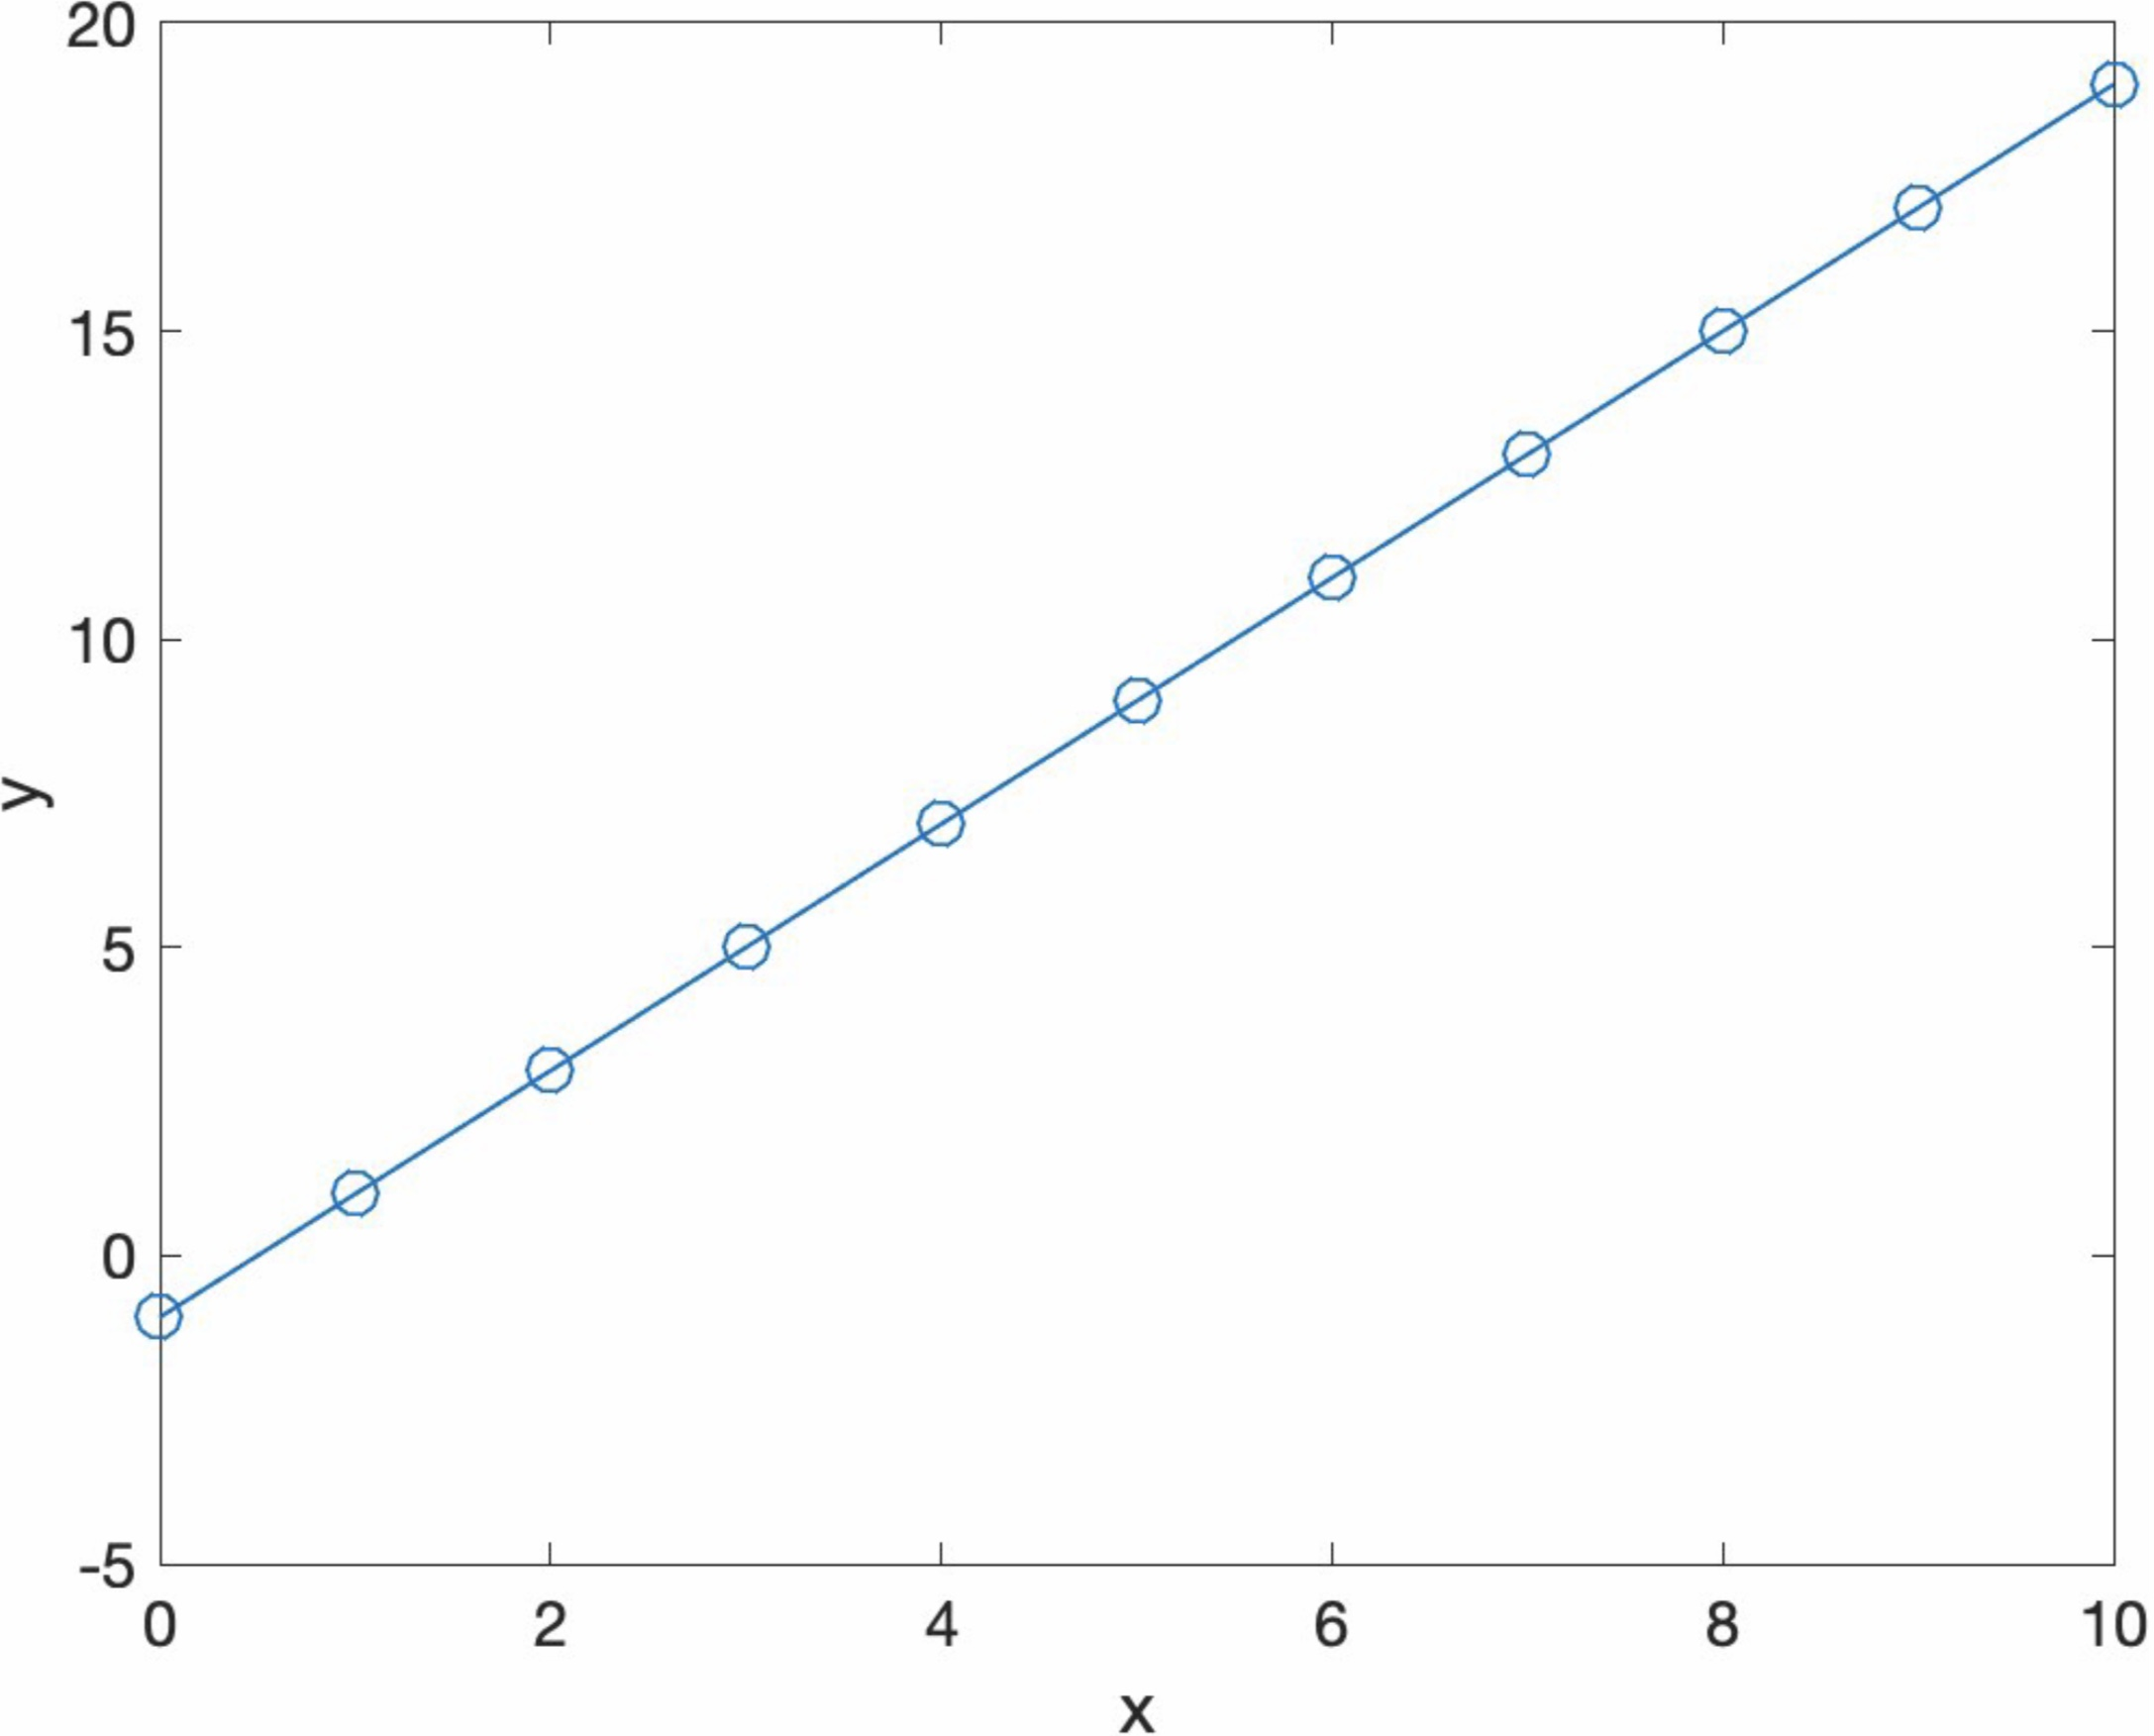
\includegraphics[width=0.5\textwidth]{immagini/4.10(1).jpg}
    \caption{Esempio di 10 dati esatti.}
    \label{fig:4.10(1)}
\end{figure}

Per la Figura \ref{fig:4.10(1)} è possibile affermare che la retta che passa per i 10 punti necessiterebbe solo di due punti per definirla e che i dati sono collineari. Se fossero interpolanti con una spline o con un polinomio interpolante sarebbe ottenuta una retta.

\begin{figure}
    \centering
    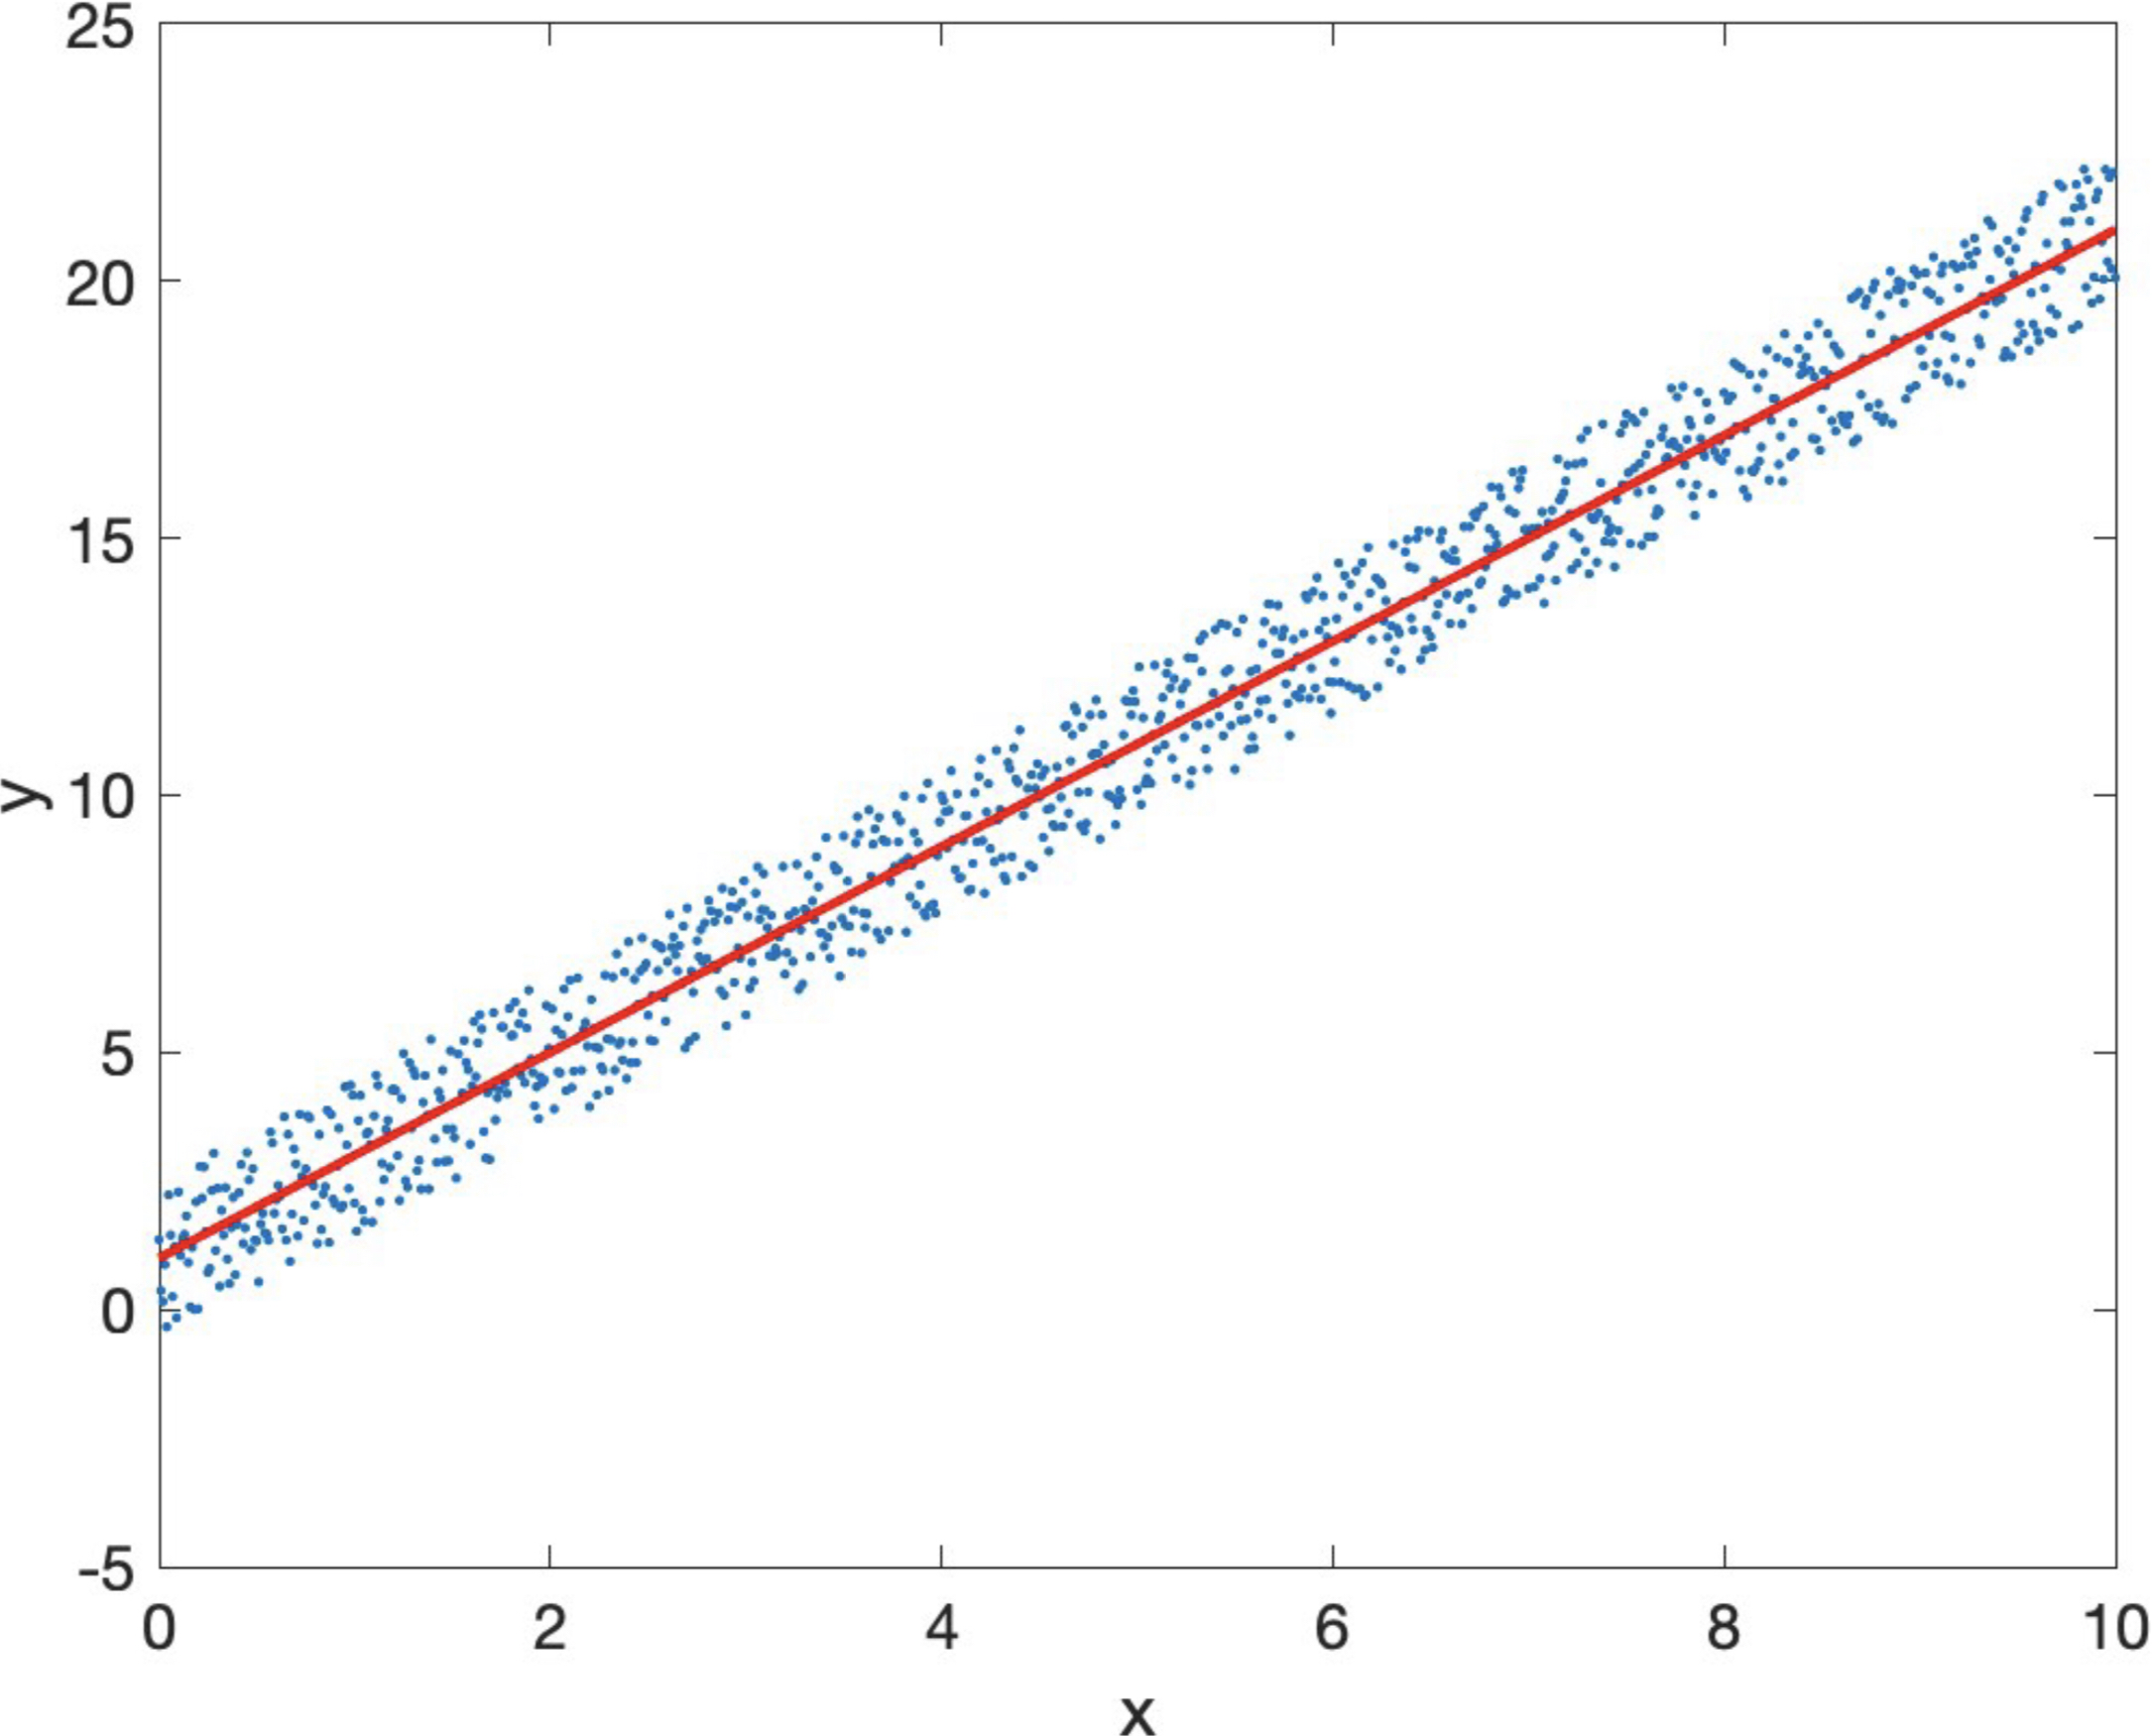
\includegraphics[width=0.5\textwidth]{immagini/4.10(2).png}
    \caption{Esempio di 1000 dati affetti da errore.}\label{fig:4.10(2)}
\end{figure}

Supposto di avere 1000 dati effetti da errore non sistematico, è ottenuta Figura \ref{fig:4.10(2)}. I dati, i puntini nella figura, sono ottenuti partendo dalla retta ed aggiungendo un termine d'errore, non lo stesso della retta, da un distribuzione gaussiana. Se fosse necessario interpolare allora il grafico oscillerebbe tra gli estremi dei puntini blu (più o meno periodicamente), non fornendo informazioni utili. La retta rossa, rappresentante la retta in Figura \ref{fig:4.10(1)}, approssima bene i dati.

\begin{figure}
    \centering
    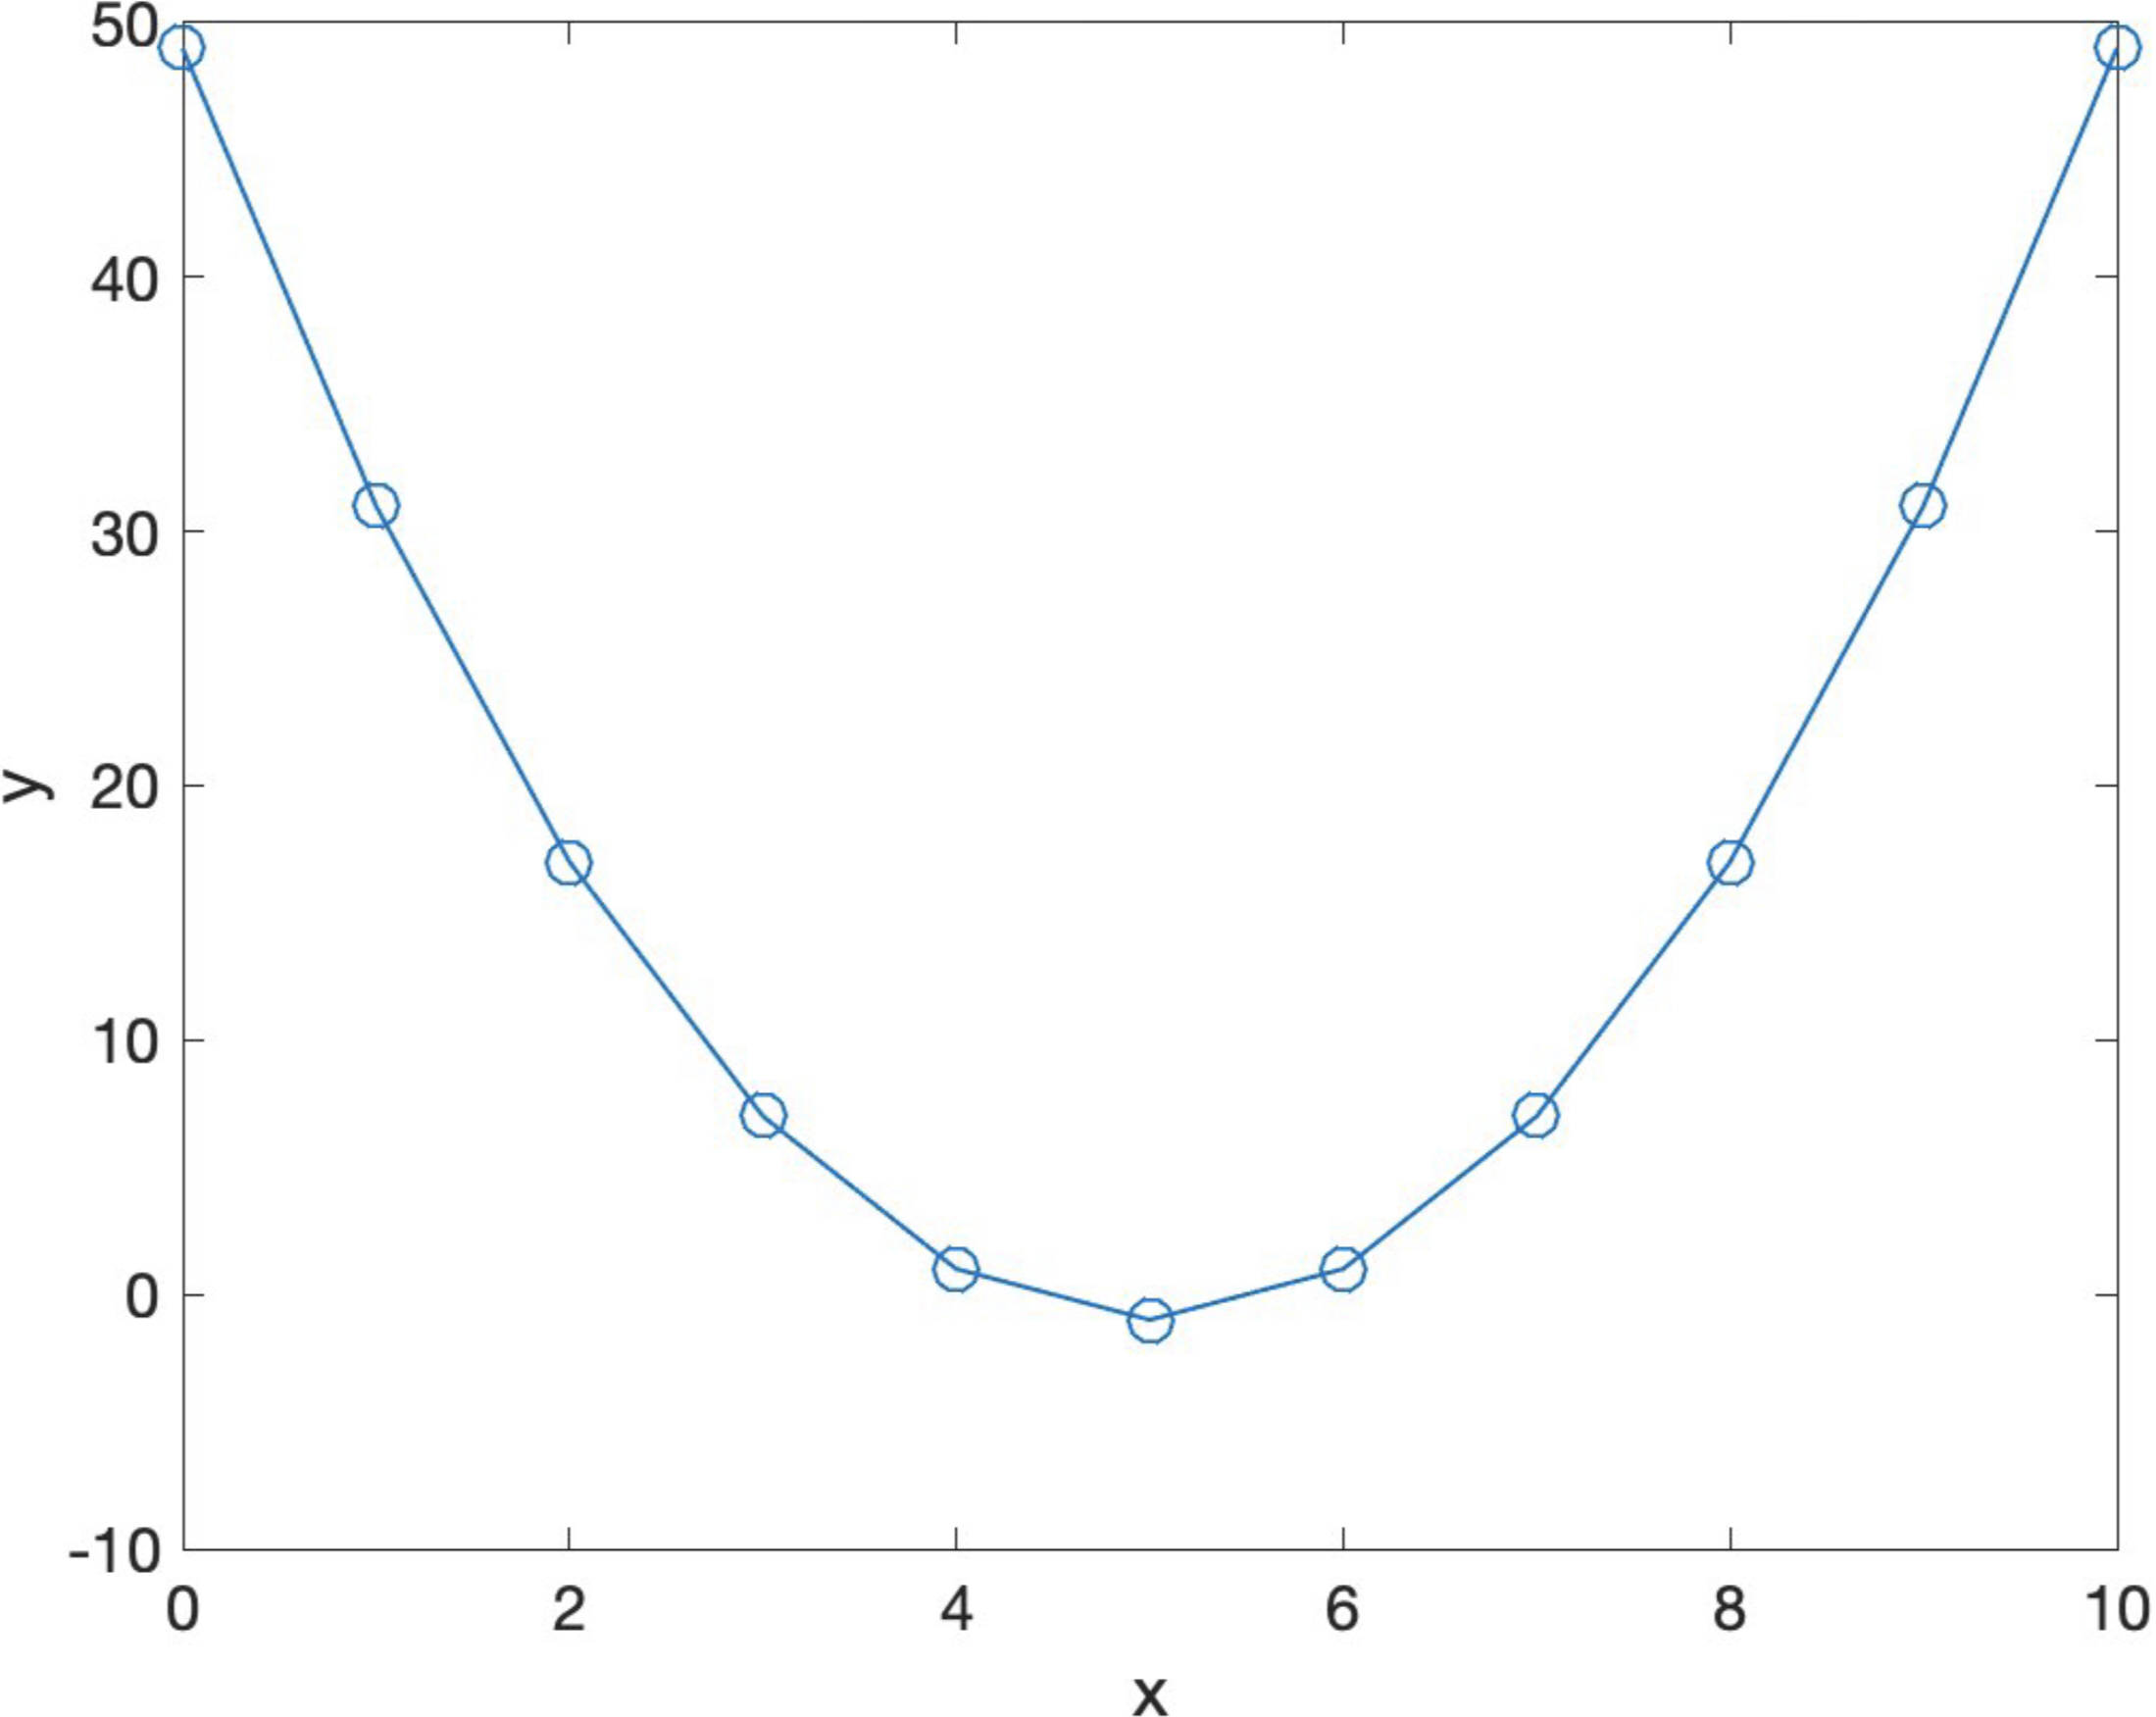
\includegraphics[width=0.5\textwidth]{immagini/4.10(3).png}
    \caption{Esempio di spline con $n=4$.}\label{fig:4.10(3)}
\end{figure}

\begin{figure}
    \centering
    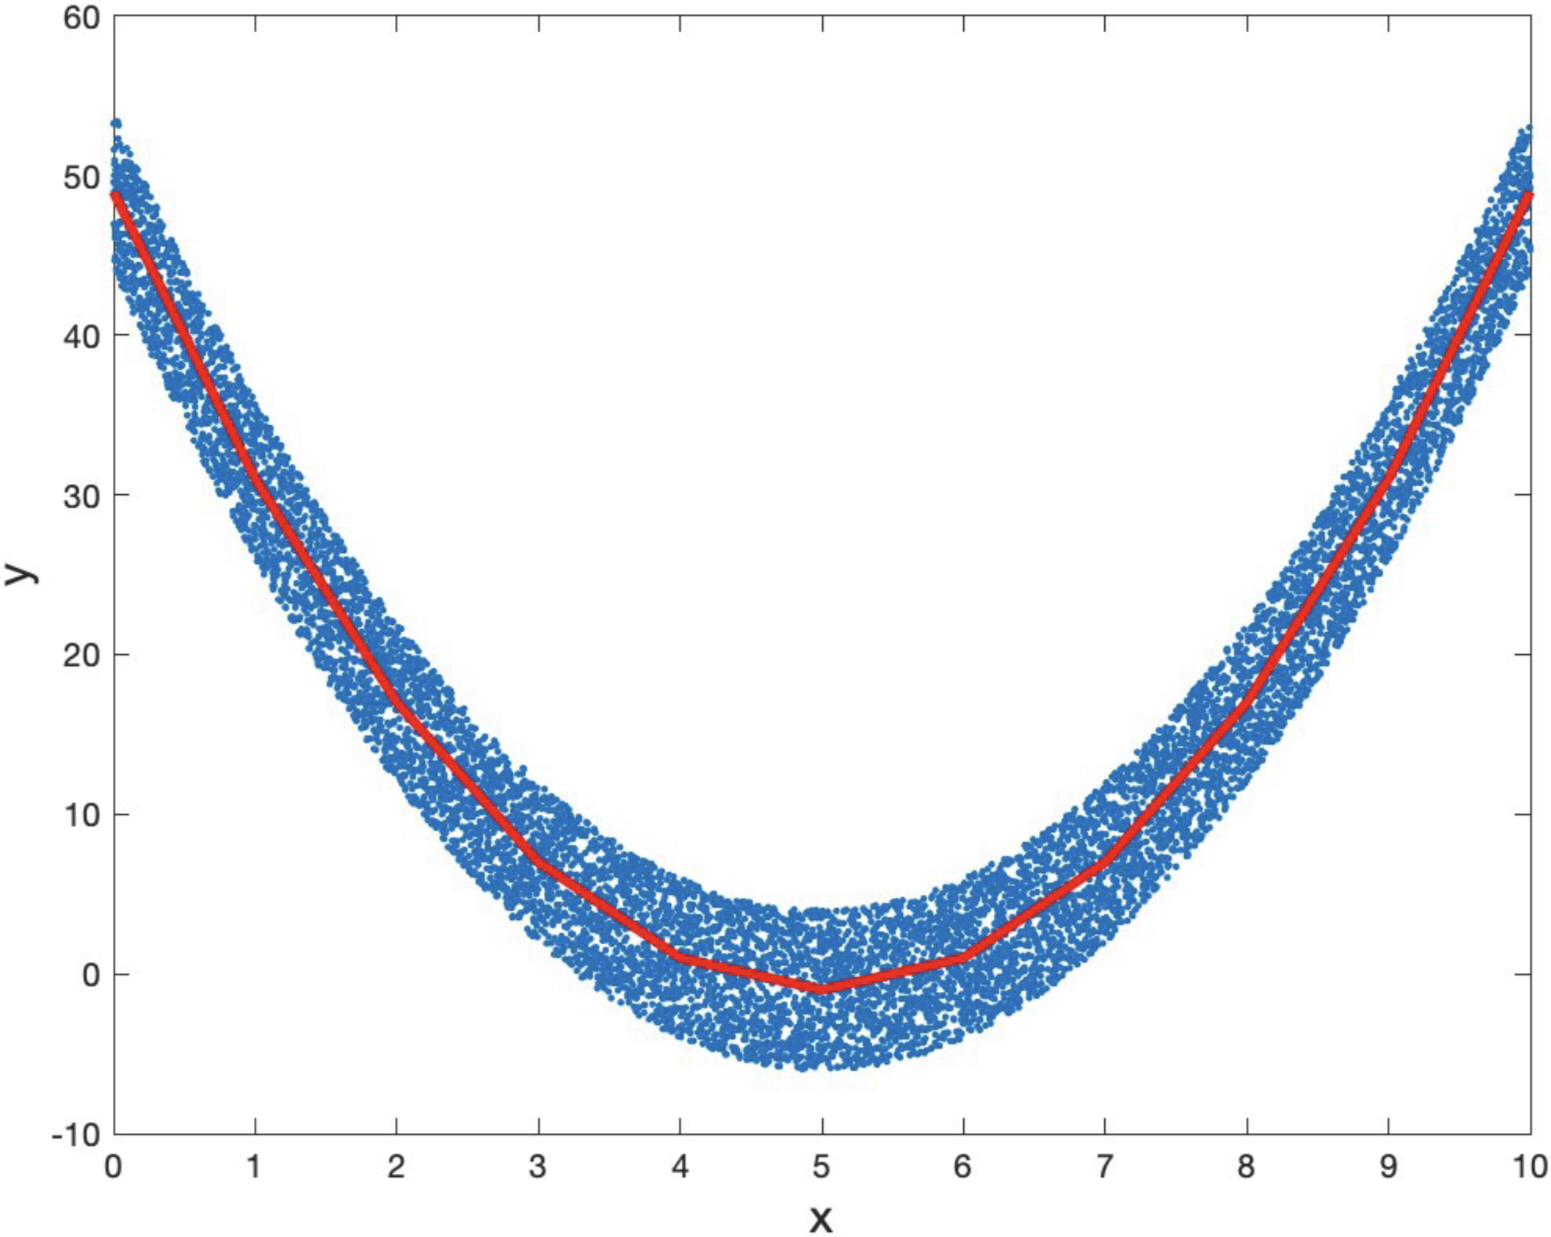
\includegraphics[width=0.5\textwidth]{immagini/4.10(4).png}
    \caption{Esempio di spline con 10000 dati.}\label{fig:4.10(4)}
\end{figure}

Per la Figura \ref{fig:4.10(4)} non ha senso calcolare il polinomio interpolante perché un polinomio di grado 10000 è impossibile da calcolare ed un polinomio si fatto non ha dati utili. Inoltre, la retta rossa della figura rappresenta la parabola di Figura \ref{fig:4.10(3)}, la quale approssima in modo soddifacente i dati.

Dalle Figure \ref{fig:4.10(1)}-\ref{fig:4.10(4)} è possibile affermare che è un caso che un punto utile sia trovato (perché sono troppi), infatti in genere non è trovato. 

Supposto di avere un fenomeno da rilevare, dipendente da un variabile indipendente $x$, che soddisfa una legge di tipo polinomiale (non inventata):
\begin{equation*}
    y=p(x),\quad p(x)\in\Pi_{\boldsymbol{m}}.
\end{equation*}

\begin{remark}
    In genere il grado $\boldsymbol m$ è noto a priori.
\end{remark}

Tuttavia, $y$, data l'uguaglianza sopra, è un polinomio del tipo
\begin{equation}\label{eq:polIgnMinQuad}
    p(x)=\sum_{k=0}^{m}a_kx^k,
\end{equation}
per il quale non sono noti i coefficienti del polinomio ma sono note le seguenti misurazioni del fenomeno:
\begin{equation}\label{eq:misFenMinQuad}
    \boldsymbol{(x_i,y_i),\quad i=1,\hdots,n,\quad n\geq m,\quad n}\overset{\footnotemark}{\boldsymbol{>>}}\boldsymbol{k+1}.
\end{equation}\footnotetext{$n$ è tipicamente molto maggiore di $k+1$, quindi il numero di misurazioni deve essere almeno pari al numero di coefficienti. Se $n=k+1$, ovvero $n$ è pari al numero di coefficienti, allora è calcolata l'interpolazione.}

\textbf{Il problema dell'approssimazione polinomiale nel senso dei minimi quadrati è determinare il polinomio (\ref{eq:polIgnMinQuad}), ovvero determinare i coefficienti} $\boldsymbol{a_0,\hdots, a_n}$\textbf{, che meglio approssima le coppie di dati definite come (\ref{eq:misFenMinQuad}).} Inoltre, è possibile osservare che il problema da risolvere è un sistema sovradimensionato ($n\geq m$).

\begin{remark}\label{re:ascDistPolm}
     È assunto che almeno $k+1$ delle ascisse $\{x_i\}$ siano distinte tra loro (dato $k$ il grado del polinomio da determinare)\footnote{Le $\{x_i\}$ possono essere utilizzate per effettuare più misurazioni in un punto in cui è necessario. È necessario che la condizione ($k+1$ ascisse distinte) sia soddisfatta per ammettere che la formulazione abbia soluzione unica.}.
\end{remark}

Per determinare i coefficienti incogniti del polinomio è necessario definire la migliore approssimazione dei dati. Il problema è rappresentato in forma vettoriale, quindi, dati i vettori
\begin{equation}
    \underline{y}=
    \begin{bmatrix}
        y_1\\
        \vdots\\
        y_n
    \end{bmatrix},\;
    \underline{z}=
    \begin{bmatrix}
        p(x_1)\\
        \vdots\\
        p(x_n)
    \end{bmatrix}
    \equiv
    \begin{bmatrix}
        \sum_{k=0}^m a_kx_1^k\\
        \vdots\\
        \sum_{k=0}^m a_kx_n^k
    \end{bmatrix},
\end{equation}
contenenti rispettivamente i valori attesi ed i valori misurati in corrispondenza delle ascisse $x_0,\hdots,x_n$, è determinato il vettore $a=(a_0,\hdots,a_m)^T$, il quale minimizza la norma $||r||_2^2=\sum_{k=0}^n|y_i-z_i|^2$ (ovvero la norma euclidea al quadrato del vettore residuo $\underline{r}=\underline{z}-\underline{y}$). Tuttavia, è possibile esprimere $\underline{z}$ come
\begin{equation*}
    \underline{z}\underset{\footnotemark}{=}
    \begin{bmatrix}
        x_1^0&\hdots &x_1^m\\
        &\vdots&\\
        x_n^0& \hdots &x_n^m
    \end{bmatrix}
    \begin{bmatrix}
        a_0\\
        \vdots\\
        a_m
    \end{bmatrix}
    \equiv V\underline{a},
\end{equation*}\footnotetext{La moltiplicazione riga di $V$ per a da la forma base di Lagrange.}con $V\in \mathbb R^{n\times k+1}$ matrice del tipo di Vandermonde. Quindi, ricercando il vettore $r$ di minima norma euclidea tale che $V\underline{a}=\underline{y}+\underline{r}$, il problema dell'approssimazione polinomiale si traduce nella ricerca della soluzione del sistema lineare sovradimensionato
\begin{equation}\label{eq:Va=y}
    V\underline{a}=\underline{y},
\end{equation}
nel senso dei minimi quadrati.

\begin{remark}
    \footnote{OSS 1 Slide 8 PDF 25.}
    $\overset{\footnotemark}{V\in\mathbb R^{n\times k+1}}$, con $n>k+1$. Questo significa che sono presenti più equazioni ($n$) che incognite ($k+1$).
\end{remark}\footnotetext{Sul libro, pagina 103, ha notazione diversa perché $n$ è indicizzato da 0, quindi è $n+1$.}

$\boldsymbol{V\underline{a}=\underline{y}}$ \textbf{è risolto tramite fattorizzazione $\boldsymbol{QR}$, sotto la condizione che la $\boldsymbol V$ abbia rango massimo ($\boldsymbol{m+1}$) affinché esista soluzione e questa sia unica.} Quindi, almeno $m+1$ delle ascisse $\{x_i\}$ devono essere distinte fra loro.

\begin{remark}
    \footnote{OSS 2 Slide 8 PDF 25, Teorema 4.12 PG 103.}
    La matrice $V$ ha rango massimo ($k+1$) sotto le ipotesi dell'Osservazione \ref{re:ascDistPolm}.
\end{remark}

Data $V$, del tipo di Vandermonde e le $k+1$ righe corrispondenti alle $k+1$ ascisse distinte, è ottenuta una matrice quadrata, la quale è una matrice di Vandermonde definita da ascisse distinte (quindi è nonsingolare). Se esiste una sottomatrice di dimensione $k+1$, ma singolare, questa ha rango massimo.

\paragraph{Fuori dalla lezione:} il vettore $\uline a$ in (\ref{eq:Va=y}) esiste ed è unico. Di conseguenza esiste ed è unico il polinomio di approssimazione ai minimi quadrati (\ref{eq:polIgnMinQuad}). Riguardo al costo computazionale per ottenere il polinomo di approssimazione ai minimi quadrati, è possibile affermare che valgono le stesse considerazioni riguardo alla fattorizzazione $QR$ fatte nelle Sezioni \ref{ssec:sistemi_lineari_sovradimensionati} e \ref{sssec:complHH}.

\begin{remark}
    \footnote{OSS 3 Slide 9 PDF 25} Pertanto, il problema è risolvibile utilizzando la fattorizzazione $V=QR$, con $Q\in\mathbb R^{n\times n}$ ortogonale e $R=\begin{pmatrix}\widehat R\\ 0\end{pmatrix}\in\mathbb R^{n\times k+1}$, dove $\widehat R\in\mathbb R^{(k+1)\times (k+1)}$, triangolare superiore e nonsingolare.
\end{remark}

\begin{remark}
    \footnote{OSS 4 Slide 8 PDF 25}
    Se $\boxed{n=k+1}$ è ottenuto il polinomio di grado $k$ che interpola $(x_i,y_i),\, i=0,\hdots,k$. 
\end{remark}

Per $n=k+1,\, V$ è quadrata ed ha rango massimo, quindi il sistema $V\uline a$ è risolvibile.

\begin{remark}
    \footnote{OSS 5 Slide 9 PDF 25, Osservazione 4.8 PG 104.} Questa tecnica di risoluzione è implementata nella funzione \textit{\textbf{polyfit}} di Matlab.
\end{remark}

\begin{remark}
    \footnote{OSS6 Slide 9 PDF 25.} Dato un sistema lineare quadrato
    \begin{equation}\label{eq:sistQuad}
        V\underline{a}=\underline{y}
    \end{equation}
    e $D$ una matrice nonsingolare, allora (\ref{eq:sistQuad}) ha la stessa soluzione di
    \begin{equation}\label{eq:sistQuadD}
        DV\underline{a}=D\underline{y}.
    \end{equation}
\end{remark}

$\overset{\footnotemark}{\text{Questo}}$ \textbf{non è più vero} se la matrice $D$ è $\overset{\footnotemark}{\text{rettangolare}}$ (perché (\ref{eq:sistQuad}) e (\ref{eq:sistQuadD}) non avrebbero più la solita soluzione). 

(\ref{eq:sistQuadD}) è utilizzato, nella pratica, calcolando $D=diag(\underline{p})$, con $\underline{p}$ vettore contenente una \textbf{distribuzione di probabilità discreta} ($\iff \underline{p}\geq 0 \,\land\, \text{sum}(\underline{p})=1$), per dare un diverso peso, $p_i$, a ciascuna equazione.

\addtocounter{footnote}{-1}
\footnotetext{È utilizzato "Questo" perché alcune volte, nella ricerca del polinomio che approssima i dati e che soddisfa nel senso dei minimi quadrati il sistema, alcuni dati sono più attendibili di altri. I dati sono pesati in base all'attendibilità, attraverso una distribuzione discreta sulle diagonali di $\underline{p}$, dove le righe corrispondenti a distribuzioni più grandi saranno più importanti di altre.}

\stepcounter{footnote}
\footnotetext{Ricavare la soluzione nel senso dei minimi quadrati del sistema lineare è diverso dal ricavare la soluzione nel senso dei minimi quadrati del sistema.}

\subsection{Risoluzione di un sistema tridiagonale}\label{ssec:risSistTridiag}

\noindent\footnote{Slide 8-10 PDF 23} È necessario, ai fini della Sezione \ref{ssec:calcSplineCub}, risolvere il sistema lineare
\begin{equation*}
    A\underline{x}=\underline{q}\in\mathbb{R}^n,
\end{equation*}

\noindent dove

\begin{equation*}
    A=
    \begin{bmatrix}
        a_1 & c_1 & & & &\\
        b_2 & a_2 & c_2 & & &\\
            & b_3 & a_3 & c_3 & &\\
            & & \ddots &\ddots & \ddots &\\
            & & & \ddots & \ddots & c_{n-1}\\
            & & & &  b_n & a_n
    \end{bmatrix}
    \in\mathbb{R}^{n\times n}
\end{equation*}
è una matrice triangolare. È supposto che questa sia fattorizzabile $LU$.

\begin{remark}\footnote{Slide 9 PDF 23.}
    È possibile \textbf{memorizzare $\boldsymbol A$ con 3 vettori (complessità lineare dei dati)}.
\end{remark}

%\hrule
%\vspace{4px}
\noindent Risolvere per fattori $LU$ ha complessità lineare. Invece di avere $\frac{2}{3}n^3$ flops per la fattorizzazione ed $n^2$ operazioni per i fattori triangolari. In questo caso la complessità è $n$ per la fattorizzazione ed $n$ per la risoluzione.

\noindent Errori da non fare: con complessità lineare è possibile risolvere problemi di qualsivoglia grandezza, con $n^2$ fino ad un certo punto e con ordine superiore al secondo no. Per risolvere il sistema tridiagonale alcune persone utilizzano una matrice piena, assegnano i tre vettori alle tre diagonali e le forniscono in input alla function di risoluzione, tramite fattorizzazione $LU$. In questo caso l'esercizio è valutato 0.
%\vspace{3px}
%\hrule
%\vspace{6px}

\noindent È necessario verificare $A$ che sia fattorizzabile $LU$, ovvero $\underset{\footnotemark}{A}=LU$, con
\footnotetext{$A$ è diagonale dominante quindi fattorizzabile $LU$.}
\begin{equation*}
    \begin{matrix}
        \underset{\footnotemark}{L}=
    \begin{bmatrix}
        1 & & & &\\
        l_2 & 1 & & &\\
        & l_3 & 1 & &\\
        & & \ddots & \ddots & &\\
        & & & l_n & 1
    \end{bmatrix}
    ,\; U\overset{\footnotemark}{=}
    \begin{bmatrix}
        d_1 & c_1 &\\
            & d_2 & c_2\\
            & & \ddots & \ddots\\
            & & & \ddots & c_{n-1}\\
            & & & & d_n
    \end{bmatrix},\\
    L\cdot U=
    \begin{bmatrix}
        d_1 & c_1 & & & &\\
        l_2d_1 & (d_2+l_2 c_1) & c_2 & & &\\
            & l_3d_2 & (d_3+l_3c_2) & c_3 & &\\
            & & \ddots &\ddots & \ddots &\\
            & & & \ddots & \ddots & c_{n-1}\\
            & & & &  l_nd_{n-1} & (d_n+l_nc_{n-1})
    \end{bmatrix}
    \end{matrix}
\end{equation*}
\addtocounter{footnote}{-1}
\footnotetext{Matrice biadiagonale memorizzabile con un vettore.}

\stepcounter{footnote}
\footnotetext{La diiagonale dei $d_i$ cambia rispetto ad A mentr la diagonale dei $c_i$ è uguale ad A.}

\noindent uguagliando gli elementi omologhi, ottenendo:\\
$d_1=a_1\\
\begin{rcases}
l_i=b_i/d_{i-1},\\
d_i=a_i-l_i\cdot c_{i-1},\; i=2,\hdots, n.
\end{rcases}$
al costo di $3n$ flops dove è possibile sovrascrivere $l_i\rightarrow b_i,\; d_i\rightarrow a_i$.

\noindent Il sistema bidiagonale per $L$ può essere risolto tramite l'utilizzo dell'Algoritmo \ref{alg:calcSistBdiagL}, con $\underline{x}\leftarrow\underline{q}$.

\begin{algorithm}\caption{Algoritmo risoluzione sistema bidiagonale per $L$}
\label{alg:calcSistBdiagL}
    \begin{lstlisting}[style=Matlab-editor]
    for i = 2 : n
        x_i = x_i - e_i x_(i - 1) % (2n flops)
    end
    \end{lstlisting}
\end{algorithm}

\noindent Il sistema bidiagonale per $U$ può essere risolto con l'Algoritmo \ref{alg:calcSistBdiagU}.
\begin{algorithm}\caption{Algoritmo risoluzione sistema bidiagonale per $U$}
\label{alg:calcSistBdiagU}
    \begin{lstlisting}[style=Matlab-editor]
    x_n = x_n / d_n
    for i = n - 1 : -1 : 1
            x_i = (x_i - c_i x_(i + 1)) / d_i %(3n flops)
    end
    \end{lstlisting}
\end{algorithm}

\noindent Quindi al posto di $\frac{2}{3}n^3$ flops c'è $3n$ ed al posto di $n^2\; 2n$. Totale $8n$ flops, mentre se è simmestrica $7$ flops.

\noindent Morale: se è richiesto di risolvere un sistema tridiagonale fattorizzabile $LU$ allora è necessario utilizzare l'Algoritmo \ref{alg:calcSistBdiagU}, non assegnando i 3 vettori ad una matrice e richiamando la function per la risoluzione fattorizzabile $LU$.

\section{Formule di quadratura numerica (approssimazione di integrali definiti)}
\footnote{Slide 10 PDF 25, 26-27, PG 105-114.}
Il problema da risolvere è quello di approssimare il valore dell'integrale nella forma
\begin{equation}\label{eq:probQuadratura}
    I(f)=\int_{a}^{b}f(x) dx,\quad -\infty<\overset{\footnotemark}{\boldsymbol{a<b}}<\infty ,
\end{equation}
dove $f:[a,b]\rightarrow\mathbb R$, almeno continua. In questa trattazione di approssimazione di integrali definiti è considerato solo il caso in cui $f$ è continua, per evitare singolarità integrabili nell'intervallo $[a,b]$ e non sarà considerato il caso di integrali definiti su insiemi illimitati. I metodi di approssimazione trattati saranno definiti mediante l'integrale di una approssimazione polinomiale a tratti di $f(x)$, in quanto l'integrale di un polinomio può essere calcolato facilmente ed in modo esatto.
\footnotetext{Se $a>b$ allora è applicato Riemann, $a$ e $b$ sono invertiti di segno. Se non è conosciuta la derivata prima di $f$, l'integrale è calcolato in forma chiusa. Spesso è necessario fornire un metodo numerico in questo intervallo. Questi metodi si chiamano "Forma di quadratura" (i quali consentono di determinare l'integrale esatto di una approssimazione della funzione $f$, per la quale è possibile l'integrazione). Prima è necessario studiare il condizionamento del problema dell'integrazione.}

Prima di trattare i metodi di approssimazione è studiato il condizionamento del problema, in cui la perturbazione è sulla funzione integranda $f(x)$. Studiare il condizionamento significa stabilire se al posto di $f$ è presente una sua perturbazione, ovvero quando il risultato è perturbato.

\begin{definition}[Numero di condizionamento]
    Supposta $\Tilde{f}(x)\in C^{(0)}[a,b]$, ovvero una perturbazione di $f(x)$, allora (vedi (\ref{eq:defNormaInfG})):
    \begin{equation*}
        \begin{matrix}
            \overbrace{\boldsymbol{|I(f)-I(\Tilde{f})|}}^{\footnotemark} &=& \left|\int_{a}^{b}f(x)dx-\int_{a}^{b}\Tilde{f}(x)dx\right| &=& \left|\int_{a}^{b}(f(x)-\Tilde{f}(x))dx\right|\\
             &\underset{\footnotemark}{\leq}&\int_{a}^{b}|f(x)-\Tilde{f}(x)|dx&\leq& ||f-\Tilde{f}||\cdot\int_{a}^{b}dx &=&\boldsymbol{(b-a)\cdot}\boldsymbol{||f-\Tilde{f}||},
        \end{matrix}
    \end{equation*}
    
    \addtocounter{footnote}{-1}
    \footnotetext{Errore del risultato.}
    
    \stepcounter{footnote}
    \footnotetext{Il valore assoluto di un integrale di una funzione è minore uguale dell'integrazione del valore assoluto della funzione. Questo è specificato anche dal criterio di integrabilità.}
    
    \noindent dove
    \begin{equation*}
        \boldsymbol{\kappa=(b-a)},\quad \boldsymbol{||f-\Tilde{f}||}=\underset{a\leq x\leq b}{\max} |f(x)-\Tilde{f}(x)|
    \end{equation*}
    definiscono, rispettivamente, il \textbf{numero di condizionamento del problema} (\ref{eq:probQuadratura}) e la misura l'\textbf{errore sui dati d'ingresso}.
\end{definition}

\subsection{Formule di Newton-Cotes}\label{ssec:formN-C}\footnote{Slide 10 PDF 25-26, PG 106-108.}
Le formule più semplici per l'approssimazione di $I(f)$ nell'intervallo $[a,b]$, dette \textbf{formule di Newton-Cotes}, sono ottenute calcolando l'integrale esatto del polinomio interpolante la funzione $f(x)$ su $n+1$ ascisse equidistanti, ovvero:
\begin{equation}\label{eq:condAscEqN-C}
    \begin{matrix}
        &x_i=a+ih,&\quad i=0,\hdots,n,\\
        &p_n(x_i)=f_i \equiv f(x_i),&\quad h=\frac{b-a}{n}.
    \end{matrix}
\end{equation}

Sia $p(x)$ il polinomio interpolante $f(x)$, è considerata la sua forma di Lagrange (\ref{eq:polLagrange})-(\ref{eq:formaKronecker}) per l'approssimazione di $I(f)$. Segue la definizione della \textbf{formula di Newton-Cotes di grado} $\boldsymbol n$ (esprimile in (\ref{eq:formN-C})):
\begin{equation*}
    I(f)\approx \int_a^b p(x)dx=\underbrace{\sum_{i=0}^n f_i\int_a^b L_{in}(x)dx}_{\footnotemark}\equiv I_n(f).
\end{equation*}\footnotetext{Questa è una formulazione ingombrante, cambiando intervallo è necessario ricalcolare gli $f_i$ (ovvero gli $f(x_i)$). Tramite la sommatoria è ottenuta una combinazione lineare dei valori della funzione $f$ pesata dagli integrali (i quali sono integrali del polinomio di Lagrange).}

Una formulazione più conveniente della precedente, poste le seguenti condizioni, per $x=a+th$ e $t\in [0,n]$:
\begin{enumerate}
    \item $\underbrace{x_i=a+ih}_{\footnotemark}\Rightarrow x_i\rightarrow i,\quad i=0,\hdots ,n$,
    \item $dx=\boldsymbol{h}dt\quad (h=\frac{b-a}{n}$, ovvero $h$ di (\ref{eq:condAscEqN-C})),
\end{enumerate}\footnotetext{Trasformazione lineare di $x=a+th$.}
è la seguente:
\begin{equation*}
    \begin{matrix}
        \int_a^b L_{in}(x)dx&=&h\int_0^nL_{in}(a+th)dt&\overset{x=a+th}{=}& h\int_0^n\prod_{j=0,j\neq i}^{n}\frac{\overbrace{(a+th)}^x-\overbrace{(a+jh)}^{x_j}}{\underbrace{(a+ih)}_{x_i}-\underbrace{(a+jh)}_{x_j}}dt\\
        &\overset{\footnotemark}{=}&h\underbrace{\int_0^n\prod_{j=0,j\neq i}^n\frac{t-j}{i-j}dt}_{c_{in}} &\equiv& \frac{b-a}{n}\, c_{in} &=& h\,c_{in}.
    \end{matrix}
\end{equation*}

\footnotetext{Semplificando $a$ e raggruppando $h$.}

Pertanto, la \textbf{formula di Newton-Cotes di grado} $\boldsymbol n$ è esprimibile come:
\begin{equation}\label{eq:formN-C}
    \boldsymbol{I_n(f)\approx h\sum_{i=0}^n f_ic_{in}},\quad \boldsymbol{c_{in}=\int_0^n\prod_{j=0, j\neq i}^n \frac{t-j}{i-j}dt.}
\end{equation}

Alcune proprietà dei coefficienti $\{c_{in}\}_{i\in\{0, \hdots,n\}}$ sono le seguenti:
\begin{enumerate}
    \item \footnotemark Dalla simmetria delle ascisse $\{x_i\}$ nell'intervallo $[a,b]$ segue che:
    \begin{equation}\label{eq:simmCoeffN-C}
        \boldsymbol{c_{in}=c_{n-i,n},\quad i=0,\hdots,n.}
    \end{equation}
    \footnotetext{Slide 13 PDF 25, PG 107. Questa proprietà deriva dal fatto che le ascisse di interpolazione sono simmetriche. Affinché la 1. valga è sufficiente che le ascisse siano simmetriche (non è richiesto che siano equidistanti).}
    \item \footnotemark \begin{equation}\label{eq:coeffN-CEq1}
        \boldsymbol{\frac{1}{n}\sum_{i=0}^{n}c_{in}=1}.
    \end{equation}
    \footnotetext{Slide 13 PDF 25, Teorema 5.1 PG 106.}
    \begin{proof}[Dimostrazione 2.]
        Se considerato $\boldsymbol{a=0},\, \boldsymbol{b=1}$ e $\boldsymbol{f(x)\equiv1}$ segue che, poiché $p(x)\equiv f(x)\equiv 1:$
        \begin{equation*}
            \int_0^1 1\cdot dx=1\equiv I_n(1)=\frac{1}{n}\sum_{i=0}^n1\cdot c_{in}=\frac{1}{n}\sum_{i=0}^nc_{in}.\quad\footnotemark
        \end{equation*}
        \footnotetext{Se $n=1$ sono presenti due coefficienti e non è necessario calcolarli perché è noto che siano uguali (la somma $c$ vale $\frac{1}{2}$). Se $n=2$ sono presenti tre coefficienti, è calcolato il primo (il quale è uguale all'ultimo) e l'altro è ottenuto tramite differenza tra il risultato e i due coefficienti uguali. Il calcolo dei coefficienti è spiegato tra poche righe.}
    \end{proof}
\end{enumerate}

Riassumendo: $I(f)\approx I(p_n)\equiv I_n(f)=\frac{b-a}{n}\sum_{i=0}^n f_i \int_0^n\prod_{j=0,j\neq i}^n\frac{t-j}{i-j}dt.$

\textbf{Utilizzando (\ref{eq:formN-C})-(\ref{eq:coeffN-CEq1}):}
\begin{enumerate}
    \item $\boldsymbol{\underline{n=1}}:\; c_{01},\, c_{11}$ sono i coefficienti (da calcolare, anche se non realmente) e dalle precedenti proprietà 1. e 2. segue che $c_{01}=c_{11}=\frac{1}{2}.$ Pertanto, quando il gardo è 1, \textbf{è definita la formula dei trapezi:}
    \begin{equation}\label{eq:formTrapezi}
        \boxed{\boldsymbol{I_1(f)=\frac{b-a}{2}(f(a)+f(b))},}
    \end{equation}
    la quale ha un importante significato geometrico, visibile in Figura \ref{fig:grafFormTrapezi}, ovvero quello di approssimare, nel caso di funzioni non negative, l'area sottesa dal grafico di $f(x)$ con quella del trapezio avente come vertici i punti $(a,0),(a,f(a)),(b,f(b)),(b,0)$.
    \item $\boldsymbol{\underline{n=2}}$: In questo caso sono presenti 3 coefficienti, ovvero $c_{02},\, c_{12}, \,c_{22},$ t.c.:
    \begin{enumerate}
        \item[P1:] $c_{02}+c_{12}+c_{22}=2$;
        \item[P2:] $c_{02}=c_{22}$ (per la sommatoria).
    \end{enumerate}
    Quindi è necessario calcolare un solo elemento, $c_{22}$, e non tre. È possibile calcolarlo come segue:
    \begin{equation*}
        \begin{matrix}
            \boldsymbol{c_{22}}&=&\int_0^2\frac{t}{2}\frac{t-1}{1}dt&=&\frac{1}{2}\int_0^2(t^2-t)dt&=&\\
            &&\frac{1}{2}\left[\frac{t^3}{3}-\frac{t^2}{2}\right]_0^2&=&\frac{1}{2}\left(\frac{8}{3}-2\right)&=&\boldsymbol{\frac{1}{3}}.
        \end{matrix}
    \end{equation*}
    Quindi $c_{02}=c_{22}=\frac{1}{3}\Rightarrow c_{12}=2-\frac{2}{3}=\frac{4}{3}$.
    La conseguenza di quanto scritto è la \textbf{formula di Simpson}, dato $x_0=a, x_2=b$ e $x_1=\frac{a+b}{2}$:
    \begin{equation}\label{eq:formSimpson}
        \boxed{\boldsymbol{I_2(f)=\frac{b-a}{6}\left(f(a)+4f\left(\frac{a+b}{2}\right)+f(b)\right)},}
    \end{equation}
\end{enumerate}

\begin{figure}
    \centering
    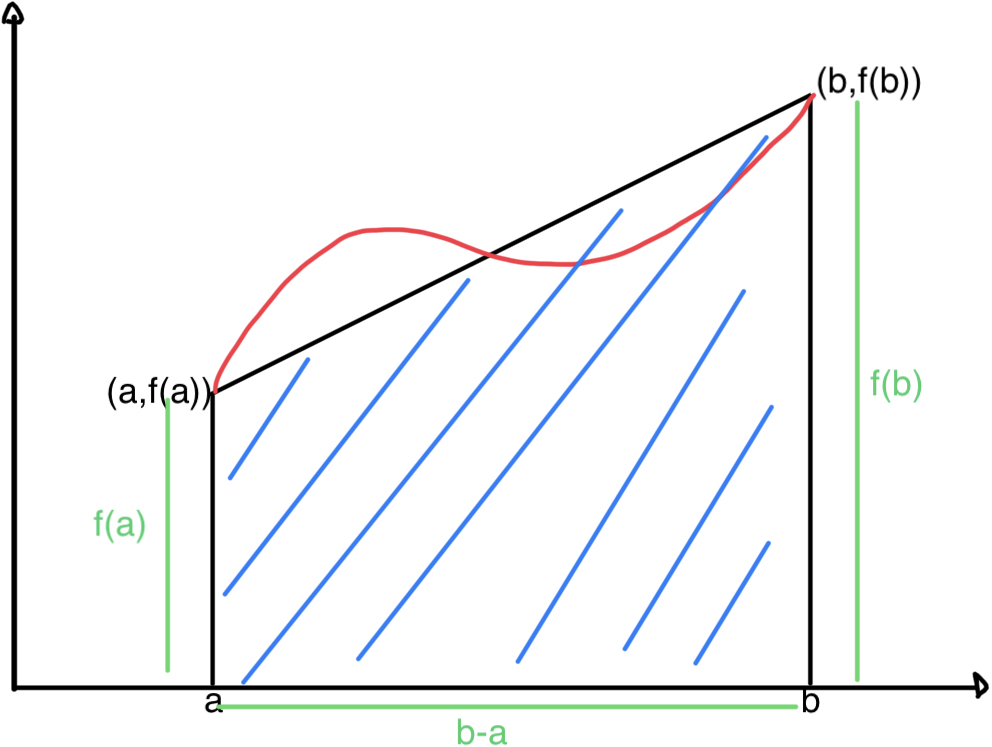
\includegraphics[width=0.5\textwidth]{immagini/grafFormTrapezi.png}
    \caption{Esempio del metodo dei trapezi ($f(a)$, $b-a$ ed $f(b)$ sono lunghezze).}\label{fig:grafFormTrapezi}
\end{figure}

\subsubsection{Condizionamento di una formula di Newton-Cotes}
\footnote{Slide 5-6 PDF 26, PG 108.}
Data una perturbazione $\Tilde{f}(x)$ di $f(x)$ e $c_{in}$, definita come in (\ref{eq:formN-C}), è possibile studiare come $\Tilde{f}(x)$ influisca su (\ref{eq:formTrapezi}), studiandone il condizionamento. In analogia con quanto visto per il condizionamento di (\ref{eq:probQuadratura}), è ottenuto quanto segue:

\begin{equation*}
    \begin{matrix}
        |I_n(f)-I_n(\Tilde{f})|&\overset{\footnotemark}{=}&\frac{b-a}{n}\left|\sum_{i=0}^n c_{in}f_i-\sum_{i=0}^n c_{in}\Tilde{f_i}\right|&=&\\
        \frac{b-a}{n}\left|\sum_{i=0}^n c_{in}\left(f_i-\Tilde{f_i}\right)\right|&\overset{\footnotemark}{\leq}&\frac{b-a}{n}\sum_{i=0}^n \left|c_{in}\left(f_i-\Tilde{f_i}\right)\right|&=&\\
        \frac{b-a}{n}\sum_{i=0}^n |c_{in}|\cdot\left|f_i-\Tilde{f_i}\right|&\leq&\left(\frac{b-a}{n}\sum_{i=0}^n|c_{in}|\right)\underset{i=0,\hdots,n}{\max}\left|f_i-\Tilde{f_i}\right|&\leq&\\
        && \underbrace{\left(\frac{b-a}{n}\sum_{i=0}^n|c_{in}|\right)}_{\boldsymbol{\kappa_n}}\cdot \equalto{\left|\left|f-\Tilde{f}\right|\right|}{\underset{a\leq x\leq b}{\max}||f(x)-\Tilde{f}(x)||}
    \end{matrix}
\end{equation*}
\addtocounter{footnote}{-1}
\footnotetext{Supposto di aver traspormato il problema in modo tale che $b>a$.}

\stepcounter{footnote}
\footnotetext{Diseguaglianza triangolare.}

\noindent dove $\boldsymbol{\kappa_n}$ è il \textbf{numero di condizionamento del problema} e $\boldsymbol{||f-\Tilde{f}||}$ misura l'\textbf{errore in ingresso}.

\begin{remark}
    \footnote{OSS Slide 6 PDF 26.} Se
    \begin{equation}\label{eq:coeffFormN-CGT0}
        \boldsymbol{\forall\, i=0,\hdots, n\; :\; c_{in}\leq 0,}
    \end{equation}
    allora:
    \begin{equation}\label{eq:nrCondN-C}
     \boldsymbol{\kappa_n}=\frac{b-a}{n}\sum_{i=0}^n|c_{in}|\overset{\footnotemark}{=}\frac{b-a}{\cancel{n}}\cancel{\sum_{i=0}^nc_{in}}\overset{\footnotemark}{=}b-a\boldsymbol{\equiv\kappa}.
    \end{equation}

\end{remark}
\addtocounter{footnote}{-1}
\footnotetext{Eliminato il modulo perché $c_{in}\geq 0$.}

\stepcounter{footnote}
\footnotetext{Per (\ref{eq:coeffN-CEq1}) ci sono le eliminazioni.}

Se i coefficienti della formula di Newton-Cotes sono non negativi allora il numero di condizionamento della formula di Newton-Cotes coincide con quello dell'integrale. Questo non significa che è ben condizionato: se l'integrale è ben condizionato allora lo è anche la funzione, se l'integrale è mal condizionato lo è anche la funzione. Ciò può essere riformulato affermando che \textbf{il mal condizionamento coincide con quello del problema continuo} (l'integrale $I(f)$).

Tuttavia, la proprietà (\ref{eq:coeffFormN-CGT0}) vale solo per $\boldsymbol{n=1,2,\hdots,7,9}$. Per tutti gli altri valori di $n$ compaiono pesi negativi ed il rapporto $\frac{\kappa_n}{\kappa}=\frac{1}{n}\sum_{i=0}^n|c_{in}|$ cresce molto rapidamente al crescere di $n$. Pertanto non è raccomandabile l'utilizzo di formule di Newton-Cotes di grado 8 o, genericamente, maggiori uguali a 10 (vedere Figura \ref{fig:knN-C}).

\begin{figure}[H]
    \centering
    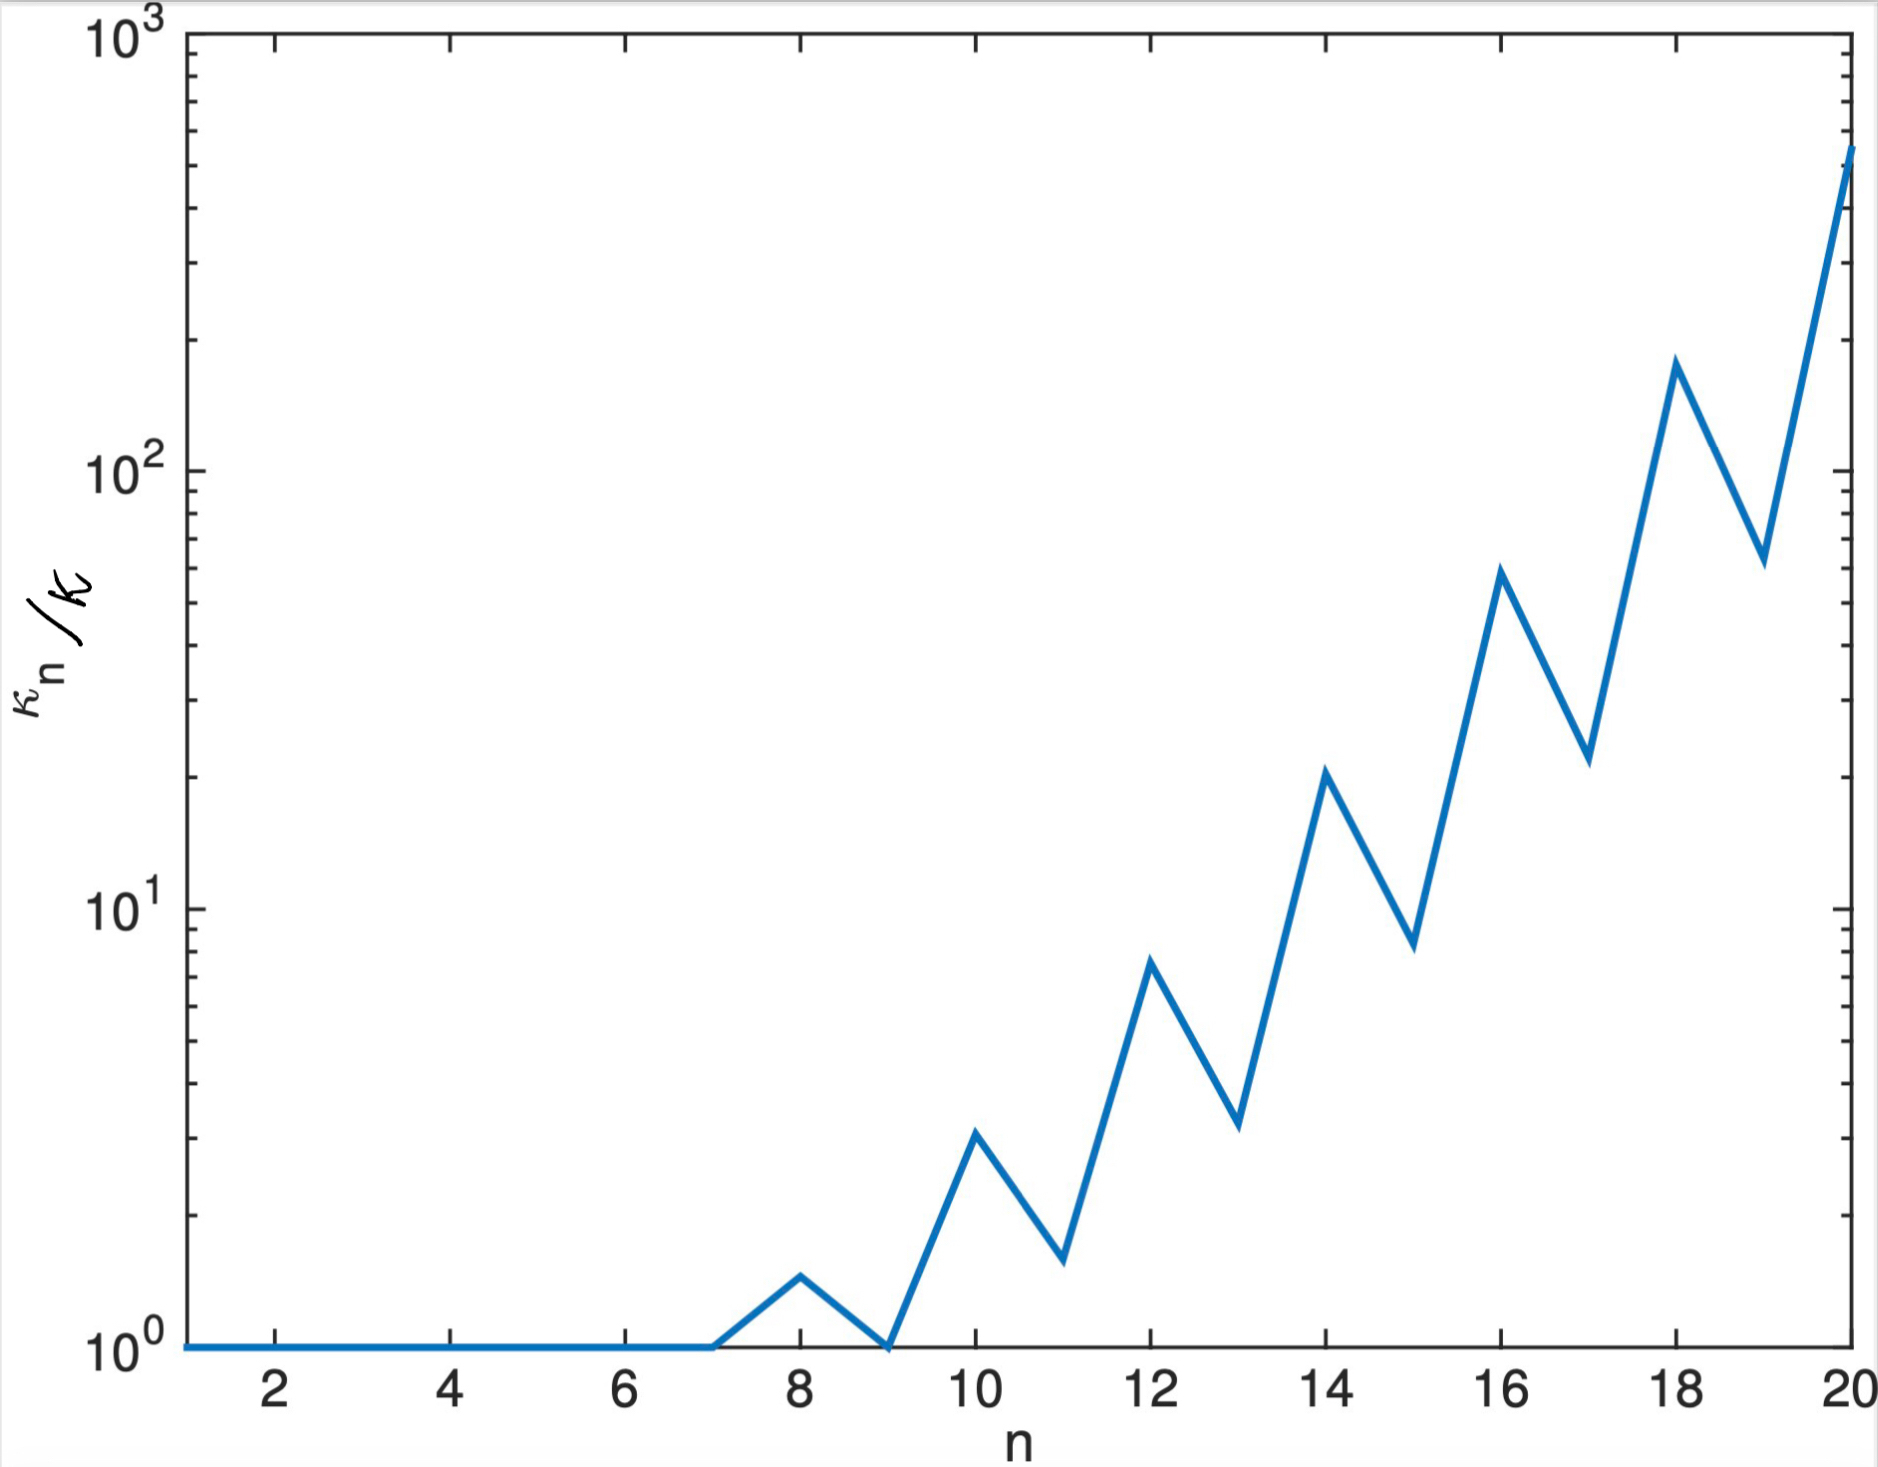
\includegraphics[width=0.5\textwidth]{immagini/knN-C.png}
    \caption{numero di condizionamento (\ref{eq:nrCondN-C}) delle formule di Newton-Cotes nel caso $b-a=1$.}\label{fig:knN-C}
\end{figure}

\subsection{Errore (di quadratura) e formule composite}
\subsubsection{Errore di quadratura}
\footnote{Slide 8 PDF 26 PG 108.} Discutere l'accuratezza di $I_n(f)$ significa quantificare l'errore di quadratura
\begin{equation}\label{eq:errQuadr}
    \begin{matrix}
        \boldsymbol{E_n(f)}&\boldsymbol{\equiv}& I(f)-\overset{\footnotemark}{I_n(f)}&=&\int_a^b f(x)dx-\int_a^bp_n(x)dx\\
        &=&\int_a^b\underbrace{(f(x)-p_n(x))}_{\footnotemark}dx&=&\int_a^bf[x_0,\hdots,x_n,x]\omega_{n+1}(x)dx\\
        &&\int_a^bf[x_0,\hdots,x_n,x]\prod_{i=0}^n(x-x_i)dx&\overset{\footnotemark}{=}&\boldsymbol{\nu_n} \underbrace{\boldsymbol{f^{(n+\mu)}(\xi)}}_{\footnotemark}\boldsymbol{\left(\frac{b-a}{n}\right)^{n+\mu+1}},\quad\xi\in [a,b],
    \end{matrix}
\end{equation}
\addtocounter{footnote}{-3}
\footnotetext{È esattamente l'integrale del polinomio interpolante la $f$.}

\stepcounter{footnote}
\footnotetext{Errore di interpolazione.}

\stepcounter{footnote}
\footnotetext{L'errore ha una struttura che nel caso $n$ sia dispari è facile da dimostrare, non è così per $n$ pari.}

\stepcounter{footnote}
\footnotetext{Assunto che $f\in C^{(n+\mu)}[a,b]$.}
\noindent dove:
\begin{itemize}
    \item $\boldsymbol{\nu_n}$ è una costante che dipende solo da $n$ (ed è limitata uniformemente);
    \item $\boldsymbol{\mu}=
    \begin{cases}
        \boldsymbol 1, &\text{se $n$ è dispari;}\\
        \boldsymbol 2, &\text{se $n$ è pari.}
    \end{cases}$
\end{itemize}

Se $n$ è dispari, è calcolata la derivata $n+1$ (dove 1 è $\mu$). Quindi la formula è esatta se è un polinomio di grado $n$, quando $n$ è dispari. Questo fatto è noto perché il polinomio di grado $n$ interpolante la funzione, la quale è un polinomio di grado $n$, coincide con la funzione stessa.

Se $n$ è pari, l'intergrale è esatto per i polinomi di grado $n+1$ e la derivata $f^{(n+\mu)}(\xi)$, con $m=2\rightarrow n+2$, si annulla se $f$ è un polinomio di grado $n+1$.

Quanto appena descritto è l'osservazione seguente.

\begin{remark}
    \footnote{Slide 10 PDF 26, Corollario 5.1 PG 110.} Una formula di Newton-Cotes di grado $n$, calcolata su $n+1$ punti, è esatta per integrandi polinomiali fino al grado:
    \begin{equation*}
        \begin{cases}
            n, &\text{se $n$ dispari};\\
            n+1, &\text{se $n$ pari}.
        \end{cases}
    \end{equation*}
\end{remark}

Dato $E_n(f)$ in forma (\ref{eq:errQuadr}) non è possibile affermare che $\left(\frac{b-a}{n}\right)^{n+\mu +1}\rightarrow 0,$ per $ n\rightarrow\infty$, a causa del condizionamento del problema. Per risolvere questo problema è necessario decrementare il rapporto $\frac{b-a}{n}$ senza fare crescere $n$, utilizzando un approccio simile a quello delle spline nel caso di interpolazione, ovvero: l'intervallo $[a,b]$ è suddiviso in più sottointervalli di uguale ampiezza ed è utilizzata, su ciascun intervallo, la formula di Newton-Cotes di grado $k$ fissato. Così facendo sono ottenute le formule di Newton-Cotes composite.
\footnote{L'idea è la seguente: date le ascisse è applicato su ciascun sottointervallo una formula di grado $k$ fissato. Con il numero di questi sottointervalli che tende all'infinito allora, la formula di grado $k$ viene applicata su intervalli sempre più piccoli. Ciò significa che il termine $\frac{b-a}{n}$ si trasformerà in $\left(\frac{b-a}{k}\right)^n$, dove $k$ è il grado della formula ed $n$ il numero di punti.}

\subsubsection{Formula dei trapezi composita}
\begin{definition}[\textbf{Formula dei trapezi composita}]\footnote{Slide 11 PDF 26.}
    Siano $\{x_i\}$ ascisse equidistanziate definite come in (\ref{eq:condAscEqN-C}), è ottenuta la \textbf{formula dei trapezi composita}:
    \begin{equation}\label{eq:formTrapComp}
        \begin{matrix}
            \boldsymbol{I(f)}&=&\int_a^b f(x) dx &\overset{\footnotemark}{=}&\sum_{i=1}^n\overbrace{\int_{x_{i-1}}^{x_i} f(x)dx}^{\footnotemark}\\
            &\approx& h\sum_{i=2}^n\frac{f(x_{i-1})+f(x_i)}{2} &\boldsymbol\equiv& \boldsymbol{I_1^{(n)}(f)}\\
            &=& h\left(\frac{f_0}{2}+\frac{f_1}{2}+\frac{f_1}{2}+\hdots +\frac{f_{n-1}}{2}+\frac{f_{n-1}}{2}+\frac{f_n}{2}\right)&\boldsymbol =&\boldsymbol{h\left(\frac{f_0}{2}+\sum_{i=1}^{n-1}f_i+\frac{f_n}{2}\right)}
        \end{matrix}
    \end{equation}
\end{definition}

\addtocounter{footnote}{-1}
\footnotetext{L'intervallo è diviso in sottointervalli e quindi l'area totale è la somma delle aree parziali, le quali sono approssimate con le funzioni trapezi.}

\stepcounter{footnote}
\footnotetext{Ogni integrale è una parte dell'area del sottografo.}

\begin{remark}
    \footnote{Slide 12 PDF 25.} Se $f(x)$ è periodica allora $f_n=f_0\Rightarrow I_1^{(n)}(f)=h\underset{\footnotemark}{\sum_{i=0}^{n-1}f_i}.$ 
\end{remark}\footnotetext{La complesità del calcolo della sommatoria è $\log (n)$ perché sommando 2 a 2 i risultati sommati 2 a 2 è possibile arrivare ad un'approssimazione in $\log (n)$ passi. Se la funzione è periodica allora è possibile approssimarla con $\sin$ e $\cos$, per le quali l'approssimazione diviene esatta, per polinomi parametrici di grado sempre più elevato, man mano che cresce $n$. Ciò significa che è possibile ottenere delle approssimazioni molto accurate di un segnale periodico (con $\sin$ e $\cos$).}

\begin{definition}[\textbf{Errore di quadratura formula dei trapezi}]
    L'\textbf{errore commesso} dalla \textbf{formula dei trapezi} è il seguente:
    \begin{equation}\label{eq:errFormTrapComp}
        \begin{matrix}
            E_1^{(n)}(f) &\overset{\footnotemark}{=}& I(f)-I_1^{(n)}(f)\\
            &\overset{\footnotemark}{=}&\nu_1 \left(\frac{b-a}{n}\right)^3 \sum_{i=1}^n f^{(2)}(\xi_i),\quad \xi_i\in[x_{i-1},x_i]\\
            &=& \nu_1 \left(\frac{b-a}{\boldsymbol n}\right)^{\boldsymbol 3}\boldsymbol n  f^{(2)}(\xi),\quad \xi\in[a,b] \\
            &=& \nu_1 \boldsymbol{(b-a)}f^{(2)}(\xi)\,\boldsymbol{\left(\frac{b-a}{n}\right)^2}\rightarrow 0,\; n\rightarrow\infty.
        \end{matrix}
    \end{equation}
\end{definition}

\addtocounter{footnote}{-1}
\footnotetext{Somma di $\sum_{i=1}^n \int_{x_{i-1}}^{x_i} f(x)dx$ e $h\sum_{i=2}^n\frac{f(x_{i-1})+f(x_i)}{2}$.}

\stepcounter{footnote}
\footnotetext{Come in seguito, vale il teorema della sommazione discreta, ovvero: data la derivata seconda continua $f^{(2)}$ (successiva all'uguale nella sommatoria) e sommando $n$ valori che appartengono ad $n$ sottointervalli contigui allora $f^{(2)}$ sarà uguale ad $n$ volte il valore della derivata seconda in un parametro dell'intervallo. Inoltre, $\nu_1=-\frac{1}{12}$, cosa non specificata a lezione. La scelta di $\nu_1$ viene fatta risolvendo un sistema di equazioni che impone che l'errore di quadratura sia nullo per funzioni polinomiali di grado $0$ e $1$. In questo caso, è possibile arrivare alla conclusione che $\nu_1=-\frac{1}{12}$ è la scelta giusta per garantire la convergenza di ordine $O\left((b-a)^3\right)$.}

\begin{remark}
    La formula dei trapezi composita può essere implementata come nell'Algoritmo \ref{alg:trapec}.
\end{remark}

\subsubsection{Formula di Simpson composita}
\begin{definition}[\textbf{Formula di Simpson composita}]
    Siano $\{x_i\}$ ascisse equidistanziate definite come in (\ref{eq:condAscEqN-C}) e dato $\boldsymbol n$ \textbf{pari}, la \textbf{formula di Simpson composita} è
    \begin{equation}\label{eq:formSimpComp}
        \begin{matrix}
            \boldsymbol{I(f)}&=&\int_a^bf(x)dx\\
            &=&\sum_{i=1}^{\frac{n}{2}}\int_{x_{2(i-1)}}^{x_{2i}}f(x)dx\\
            &\overset{\footnotemark}{\approx}&\frac{b-a}{3\cdot n}\sum_{i=1}^{\frac{n}{2}}(f(x_{2(i-1)})+4f(x_{2i-1})+f(x_{2i}))\\
            &\underset{\footnotemark}{=}&\frac{b-a}{3n}(\underline{f_0+4f_1+f_2}+\underline{f_2+4f_3+f_4}+\hdots+\underline{f_{n-2}+4f_{n-1}+f_n})\\
            &=&\frac{b-a}{3n}\underbrace{\left[4\sum_{i=1}^{\frac{n}{2}}f_{2i-1}+2\sum_{i=0}^{\frac{n}{2}}f_{2i}-f_0-f_n\right]}_{\footnotemark}&\boldsymbol\equiv& \boldsymbol{I_2^{(n)}(f)}.
        \end{matrix}
    \end{equation}
\end{definition}

\addtocounter{footnote}{-2}
\footnotetext{Approssimazione che necessita di 3 ascisse, ovvero da $x_0$ a $x_1$, da $x_2$ a $x_4$ e così via, dove l'ascissa in mezzo è quella pesata con 4.}

\stepcounter{footnote}
\footnotetext{4 è associato ai numeri con indice dispari ($f_1,\, f_3,\hdots,\, f_{n-1})$. Gli elementi con indice pari, tranne il primo e l'ultimo, hanno coefficiente 2 perché appartenenti a due intervalli congiunti.}

\stepcounter{footnote}
\footnotetext{Quando le sommatorie dovranno essere implementate in Matlab sarà necessario sfruttare le capacità di calcolo vettoriale di Matlab. Non sono necessari cicli ma è possibile calcolare una valutazione vettoriale della $f$ su tutte le ascisse per poi pesare le componenti in modo opportuno. Sarà visto un esempio nelle esercitazioni.}

\begin{definition}[\textbf{Errore di quadratura formula di Simpson}]
    L'\textbf{errore commesso} dalla \textbf{formula di Simpson} è il seguente:
    \begin{equation}\label{eq:errFormSimpComp}
        E_2^{(n)}(f)=I(f)-I_2^{(n)}(f)=\nu_2 f^{(4)}(\xi)\left(\frac{b-a}{n}\right)^5 = \nu_2f^{(4)}(\xi)\frac{b-a}{2}\left(\frac{b-a}{n}\right)^{\overset{\footnotemark}{4}}\rightarrow 0,\; n\rightarrow\infty,\quad \xi\in[a,b],
    \end{equation}
    dove $\nu_2 = -\frac{1}{180}$ (cosa non speficiata a lezione).
    \footnotetext{$\frac{n}{2}=\frac{2}{2}+\mu=2+1$, con $n$ numero di termini.}
\end{definition}

Questa procedura si generalizza per tutte le formule di Newton-Cotes di grado $k$, a patto che $n$ sia un multiplo di $k$, ottenendo la formula di Newton-Cotes di grado $k$ è espressa come
\begin{equation*}
    I_k^{(n)}=h\sum_{i=0}^nf_ic_{ik}=h\sum_{i=0}^nf_i\int_0^k\prod_{j=0, j\neq i}^k\frac{t-j}{i-j},
\end{equation*}
e l'errore associato come
\begin{equation}\label{eq:EkComposite}
 E_k^{(n)}(f)=\nu_kf^{(k+\mu)}(\xi)\frac{b-a}{k}\left(\frac{b-a}{n}\right)^{k+\mu}, \quad \xi\in[a,b],
\end{equation}
dove $E_k^{(n)}(f)\rightarrow 0,\, n\rightarrow\infty$.

\paragraph{Spiegazione notazione $\boldsymbol{E_k^{(n)}(f)}$:} $k$ è il grado della formula base, $n$ sono i punti utilizzati sui quali è applicata la formula di quadratura composita. Ciò significa che per far diminuire l'errore è possibile far aumentare $n$ lasciando $k$ fisso.

\begin{example}
    Come esempio, esplicato tramite la Figura \ref{fig:approxIntSinx}, è approssimato tramite la formula composita dei trapezi e con quella di Simpson il seguente integrale:
    \begin{equation}\label{eq:approxIntSinx}
        \int_0^\pi \sin{x}dx\quad (=2).
    \end{equation}
    Dalla Figura \ref{fig:approxIntSinx} è possibile notare che l'approssimazione di Simpson sia migliore di quella dei trapezi perché più precisa.
\end{example}

\begin{figure}
    \centering
    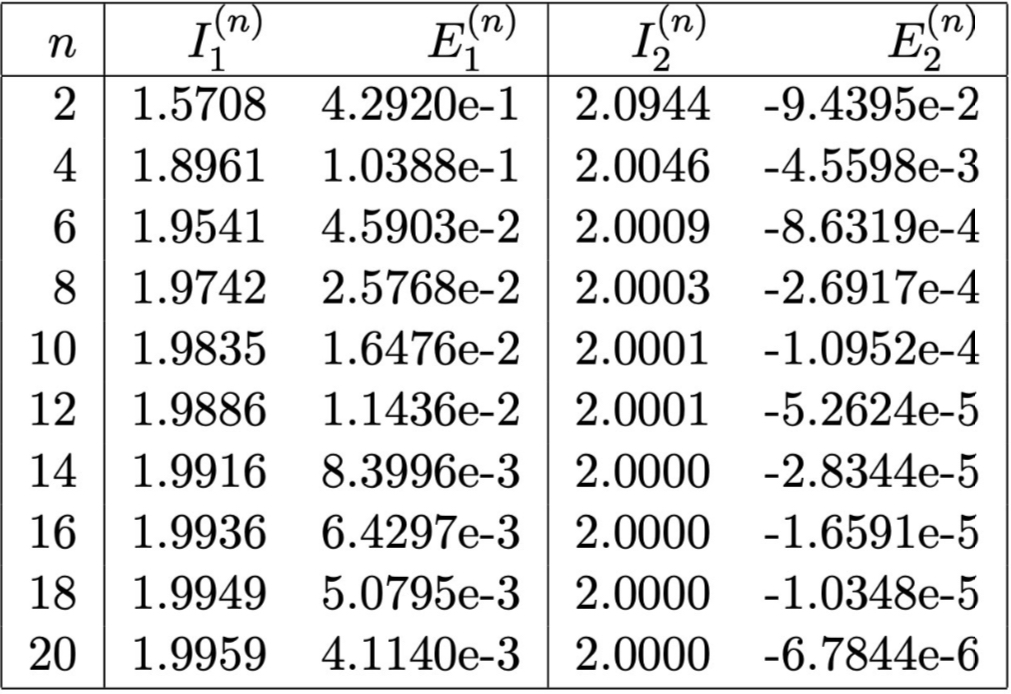
\includegraphics[width=0.5\textwidth]{immagini/approxIntSinx.png}
    \caption{Approssimazione e corrispondenti errori di (\ref{eq:approxIntSinx}).}\label{fig:approxIntSinx}
\end{figure}

L'espressione (\ref{eq:EkComposite}) permette di derivare, \textbf{a costo nullo} (cosa importante), una stima dell'errore di quadratura, $E_k^{(n)}(f)$, nel caso in cui $\boldsymbol n$ \textbf{sia un multiplo pari di} $\boldsymbol k$.

È necessario che $n$ sia un multiplo di $k$, affinché lo sia anche $\frac{n}{2}$, cosicché sia possibile valutare $\boldsymbol{I_k^{(\frac{n}{2})}(f)}$. $\boldsymbol{I_k^{(\frac{n}{2})}(f)}$ è calcolato su ascisse di indice pari ($0,2,4,\hdots$) e la valutazione di $I_k^{(\frac{n}{2}}(f)$ è ottenuta senza ulteriori valutazioni della funzione $f(x)$ perché è possibile utilizzare le valutazioni
\begin{equation*}
    \boldsymbol{f_{2i}\equiv f(x_{2i}),\quad i=0,\hdots,\frac{n}{2}},
\end{equation*}
le quali sono già calcolate per la valutazione di $I_k^{(n)}(f)$. \footnote{Sono calcolate le valutazioni funzionali di $f$ per calcolare $I_n^k(f)$ e utilizzate quelle con indice pari così da calcolare $I_n^k$. Il costo della formula di quadratura è maggiorato in un numero di valutazioni di funzioni con costo nullo.} Pertanto, analogamente a (\ref{eq:errFormSimpComp}), vale:
\begin{equation}\label{eq:errFormSimpCompN/2}
    I(f)-I_k^{(\frac{n}{2})}(f)=\nu_k f^{(n+\mu)}(\into{\widehat\xi}{[a,b]})\frac{b-a}{k}\left(\frac{b-a}{n/2}\right)^{n+\mu}\overset{\footnotemark}{\approx}\nu_k f^{(n+\mu)}(\xi)\frac{b-a}{k}\left(\frac{b-a}{n}\right)^{n+\mu}2^{n+\mu}.
\end{equation}\footnotetext{Fingendo che $\widehat\xi=\xi$ e trasformando $\frac{n}{2}$ in $2^{n+\mu}$ allora è possibile l'approssimazione.}

Sottraendo membro a membro (\ref{eq:EkComposite}) a (\ref{eq:errFormSimpCompN/2}) allora:
\begin{equation*}
    I_k^{(n)}(f)-I_k^{(\frac{n}{2})}\approx\boldsymbol{\nu_kf^{(n+\mu)}(\xi)\frac{b-a}{k}\left(\frac{b-a}{n}\right)^{n+\mu}}(2^{n+\mu}-1)\equiv \left(\boldsymbol{I(f)-I_k^{(n)}(f)}\right)(2^{n+\mu}-1).
\end{equation*}

In altri termini, è possibile ottenere una stima dell'errore di quadratura $E_k^{(n)}(f)$ come:
\begin{equation*}
    \boldsymbol{E_k^{(n)}(f)\approx\frac{I_k^{(n)}(f)-I_k^{(\frac{n}{2})}(f)}{2^{n+\mu}-1}\equiv\widehat E_k^{(n)}(f)}.
\end{equation*}

Applicando quanto scritto all'esempio (\ref{eq:approxIntSinx}) sono derivate le Figure \ref{fig:approxInt}-\ref{fig:tabErrQuad}.

\begin{figure}
    \centering
    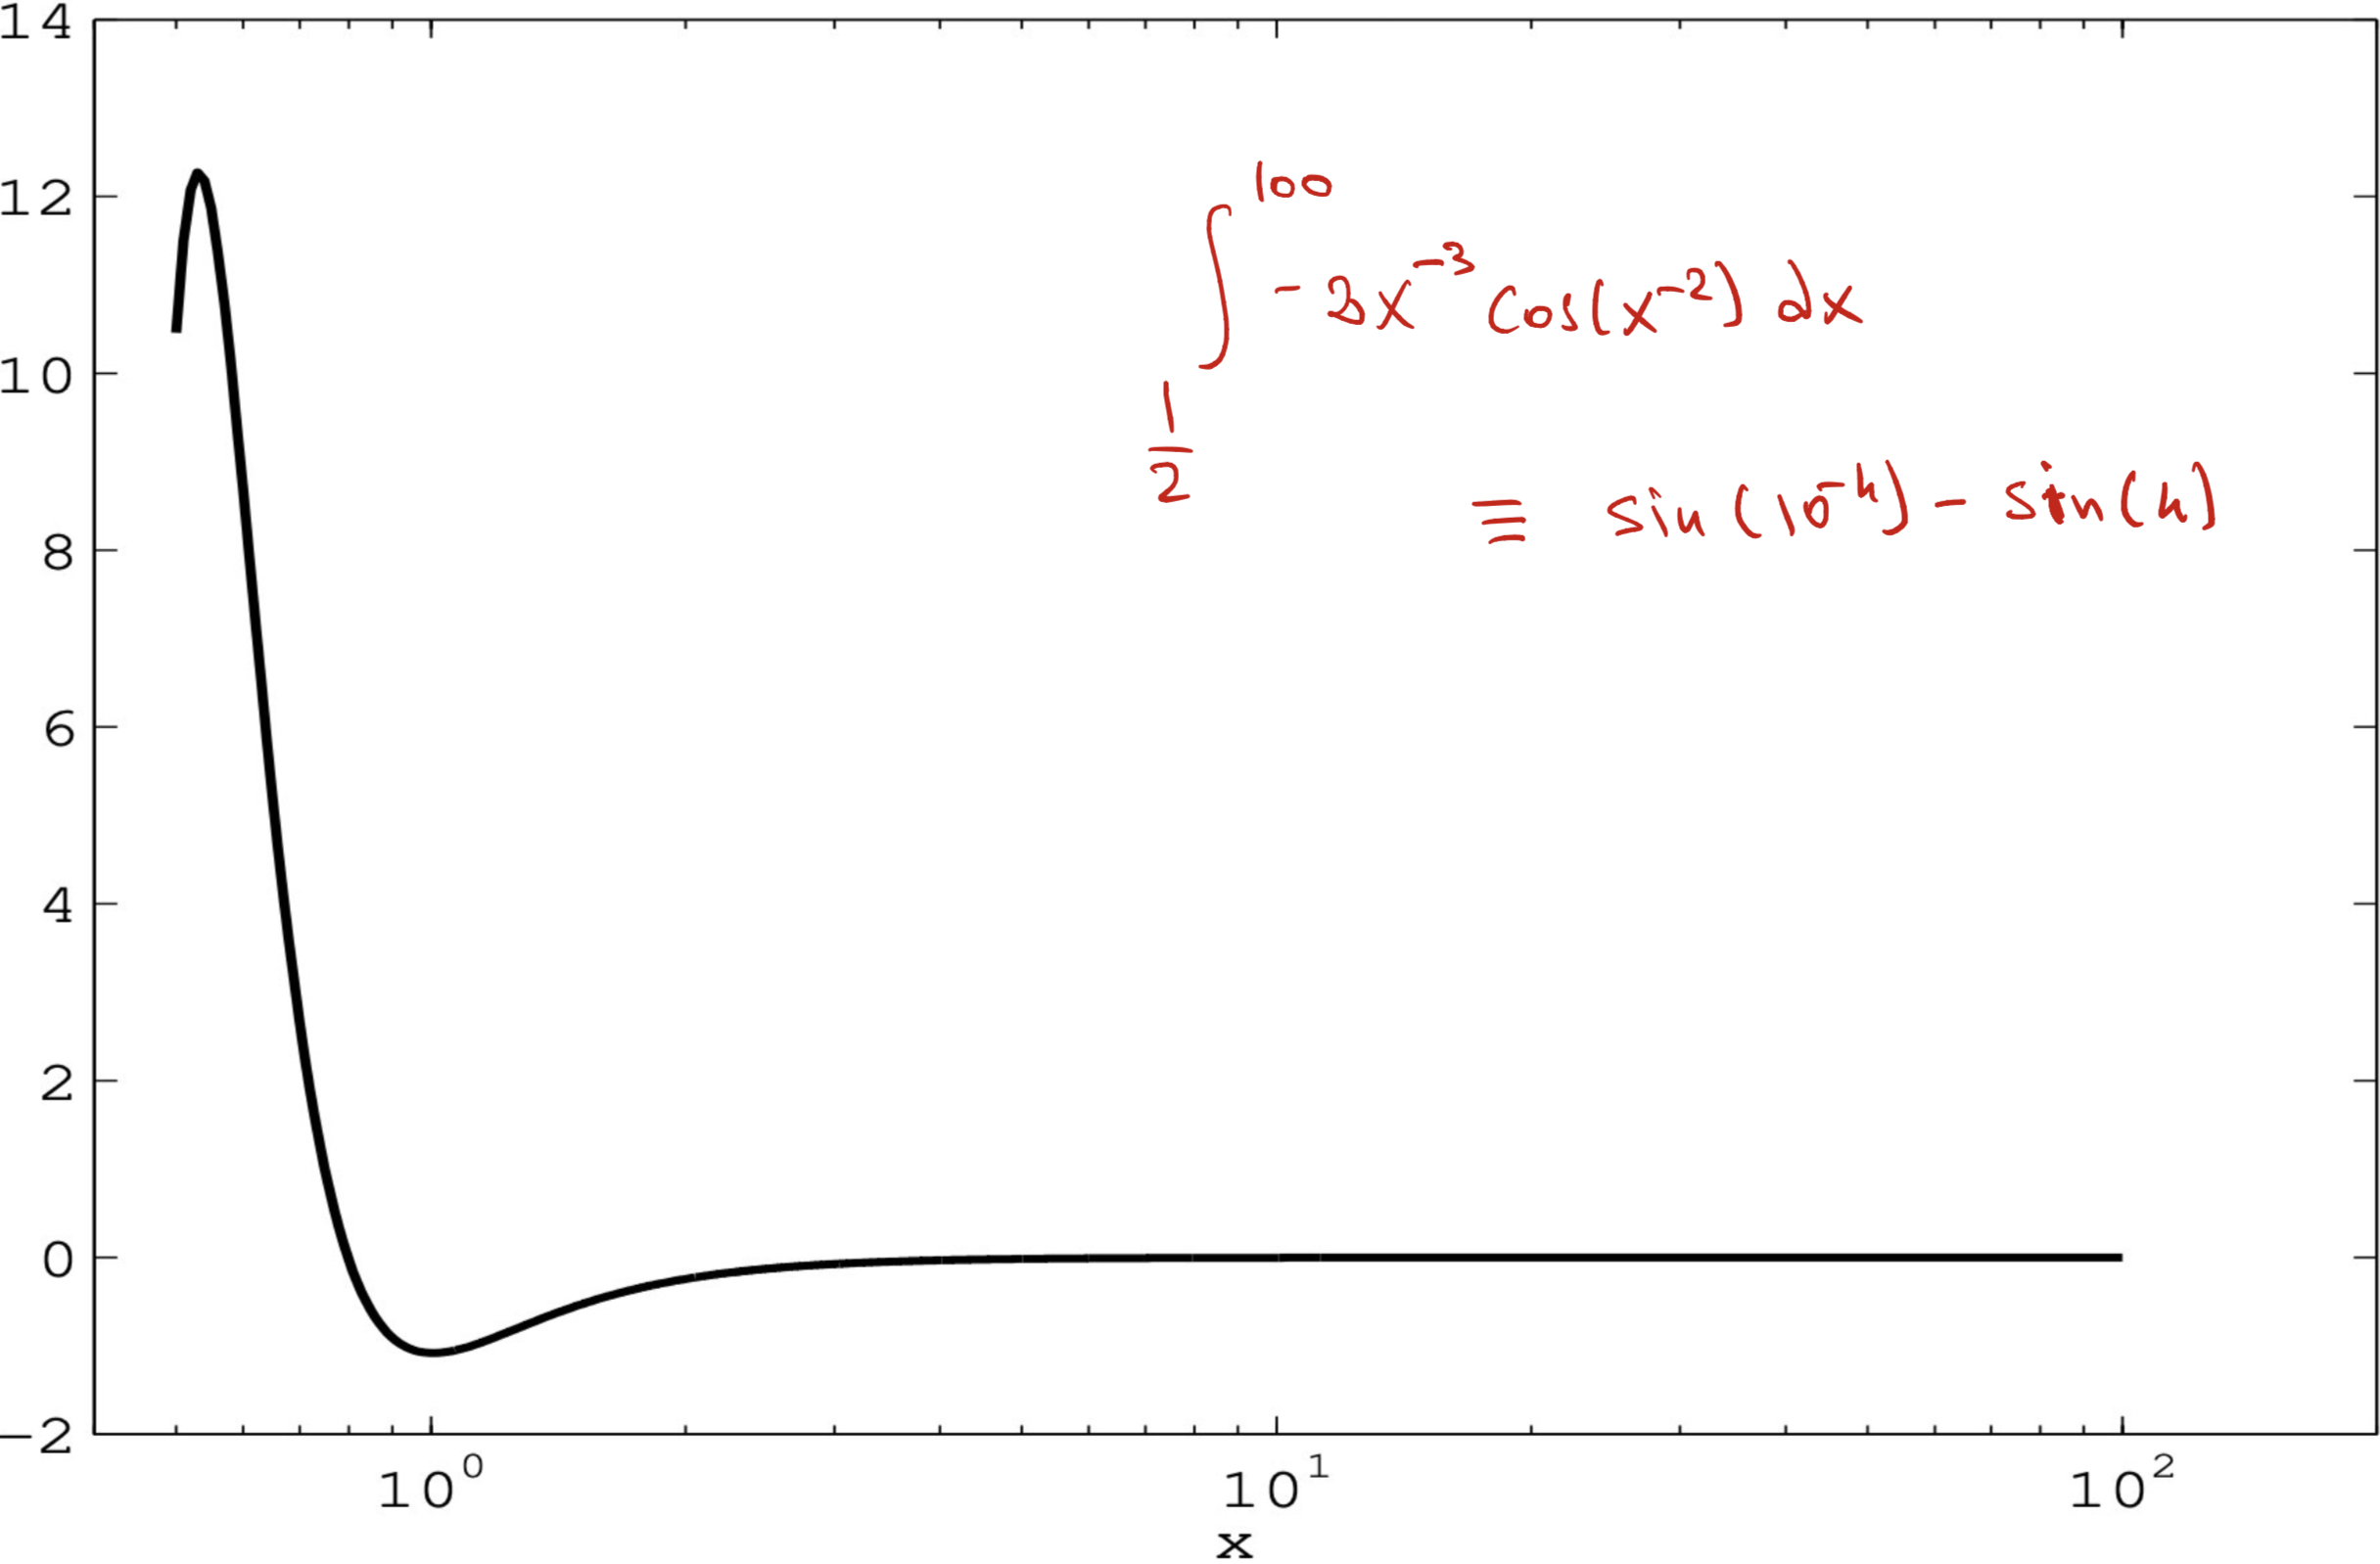
\includegraphics[width=0.5\textwidth]{immagini/approxInt.jpg}
    \caption{Approssimazione $\int_{\frac{1}{2}}^{100}-2x^{-3}\cos(x^{-2})$.}\label{fig:approxInt}
\end{figure}

\begin{figure}
    \centering
    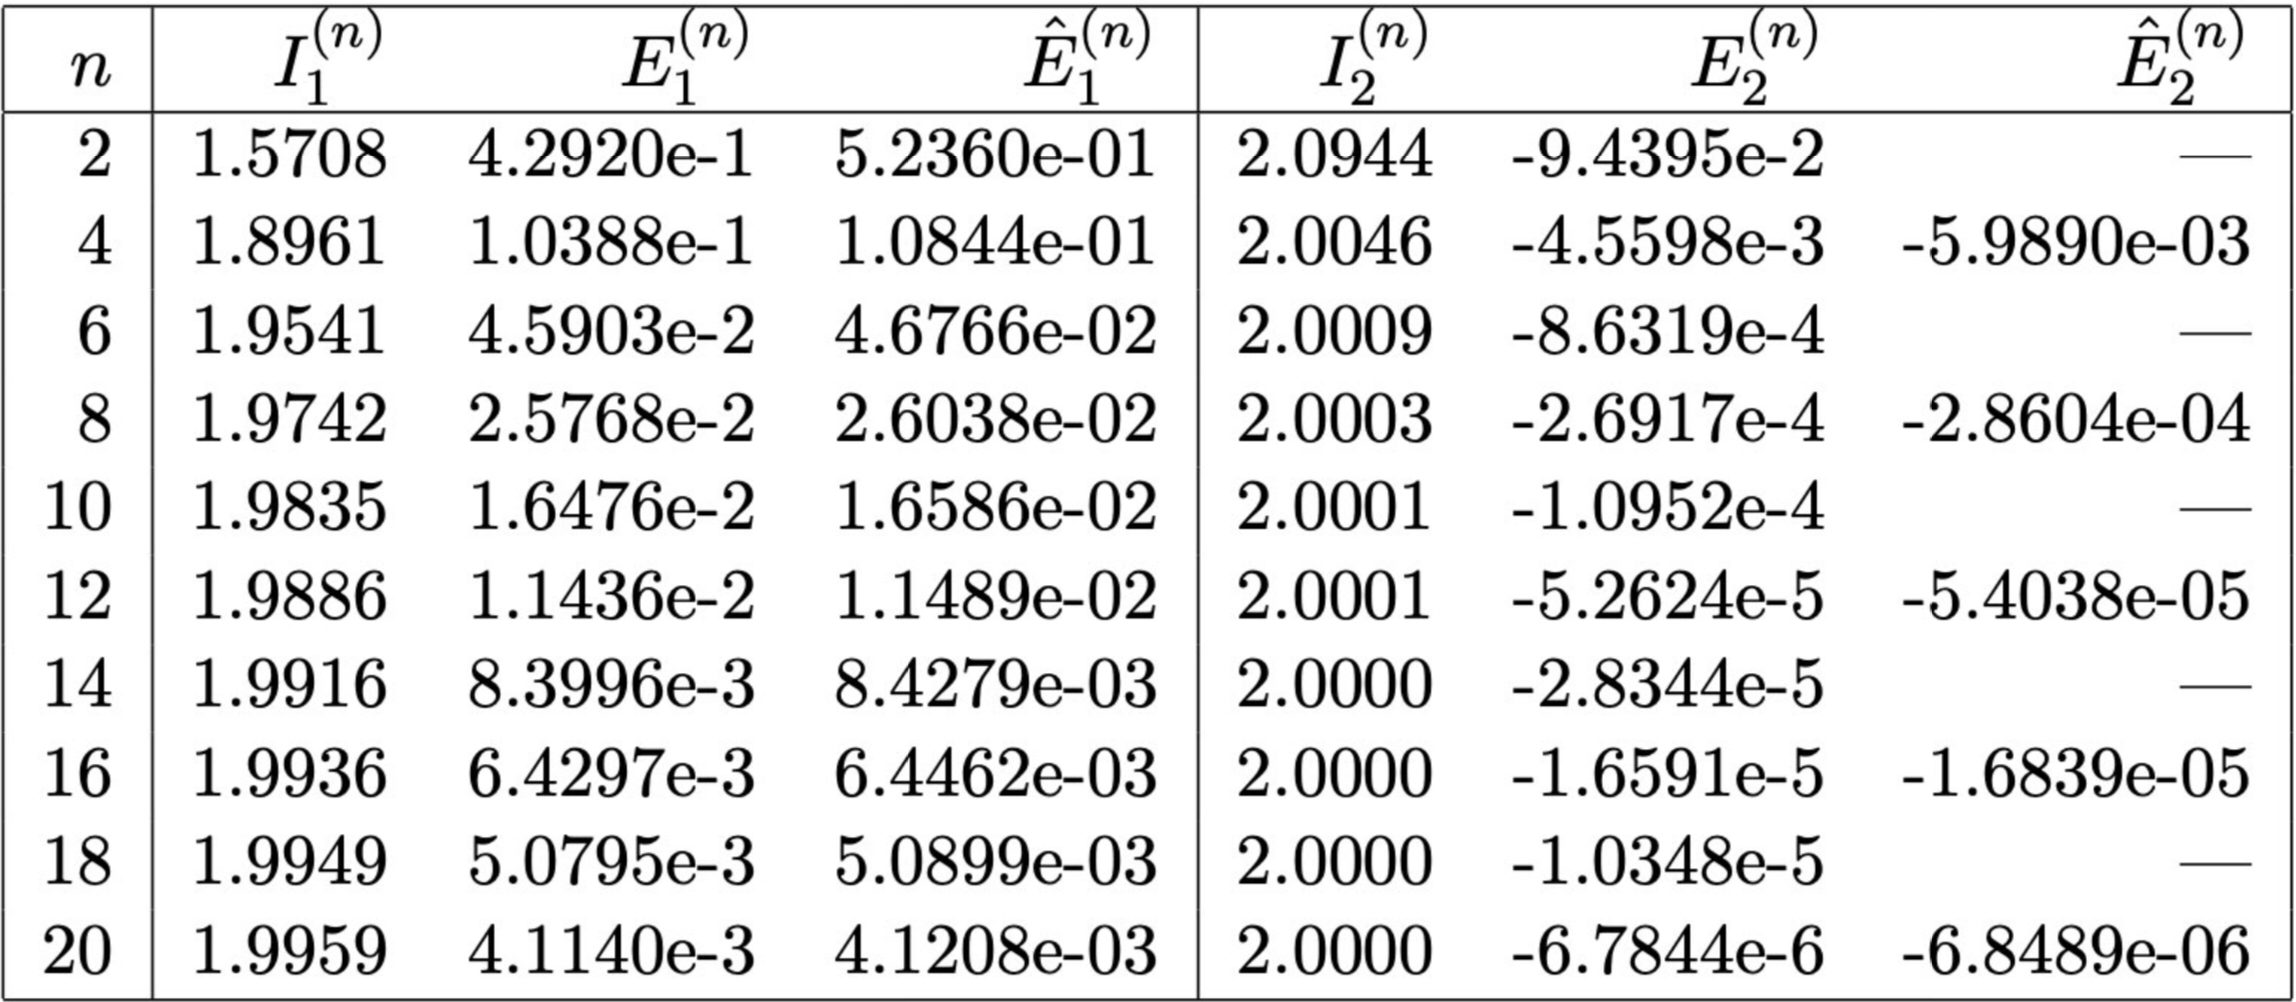
\includegraphics[width=0.5\textwidth]{immagini/tabErrQuad.png}
    \caption{Confronto fra errore di quadratura approssimazione con formula di quadratura dei trapezi e di Simpson.}\label{fig:tabErrQuad}
\end{figure}

In Figura \ref{fig:approxInt} il numero di condizionamento è 99.5, ovvero l'ampiezza dell'intervallo. Il problema è che nell'estremo inferiore, se $x\rightarrow 0$, allora $x^{-2}$ e $x^{-3}$ diventano molto grandi e $\cos{(x^{-2})}$, per $x\rightarrow 0$, oscilla molto. La parte sinistra del grafico è la parte in cui il grafico inizia ad oscillare molto. La questione importante è che la funzione è liscia poco dopo $10^0$ e oscilla poco prima di $10^0$. Se fosse utilizzata una mesh costante accadrebbe che, per ottenere la tolleranza desiderata, diventerebbero necessari punti molto vicini prima di $10^0$, i quali dovrebbero essere riportati anche nella parte liscia. Il problema posto è quello di definire un approccio adattivo per la definizione delle ascisse di interpolazione in modo adattivo, infatti sui punti laddove la funzione è più variabile saranno inseriti più punti ed invece meno dove la funzione è liscia. Per quanto appena scritto, sono introdotte le funzioni di Newton-Cotes adattive della Sezione \ref{ssec:formN-CAdatt}.
In Figura \ref{fig:tabErrQuad} è possibile notare che tanto più cresce $n$ più l'errore diminuisce e quindi aumenta la precisione. È necessario trattare il fatto che, nell'implementazione di queste formule, le ascisse sono tutte equidistanti. Le ascisse equidistanti sono definite come (\ref{eq:condAscEqN-C}).

\subsection{Formule di Newton-Cotes adattive}\label{ssec:formN-CAdatt}
\footnote{Slide 7-12 PDF 27, PG 111-114.}
Il problema è trovare un metodo per definire le ascisse in base al comportamento della funzione. Dal punto di vista algoritmico è interessante ciò che sarà visto nell'implementazione dei casi più semplici, ovvero dei trapezi e di Simpson, con Matlab, tramite function ricorsive. In ogni caso è sfruttato il fatto he esiste un'espressione asintotica dell'errore quadratico.

\subsubsection{Formula dei trapezi}
In questo caso, con $n=1$, è ottenuto (da (\ref{eq:errQuadr}))
\begin{equation}\label{eq:errQuadN=1}
    I(f)-I_1(f)=\nu_1 f^{(2)}(\xi)(b-a)^3\quad \xi\in[a,b],
\end{equation}
ed è ottenuto che, da (\ref{eq:errFormTrapComp}), applicando la formula composita su due sottointervalli ($n=2$), ciò che segue:\begin{equation}\label{eq:errQuadN=2}
    I(f)-I_1^{(2)}(f)=\nu_1 f^{(2)}(\xi)(b-a)\left(\frac{b-a}{2}\right)^2,\quad \xi\in [a,b],
\end{equation}
dove $\nu_1=-\frac{1}{12}$

Suppondendo che gli $\xi$ di (\ref{eq:errQuadN=2}) da (\ref{eq:errQuadN=1}) siano simili, sottraendo (\ref{eq:errQuadN=2}) da (\ref{eq:errQuadN=1}) è ottenuto che
\begin{equation*}
    \boldsymbol{I_1^{(2)}(f)-I_1(f)}\approx\nu_1 f^{(2)}(\xi)(b-a)\left(\frac{b-a}{2}\right)^2\underset{\footnotemark}{(4-1)}\equiv \left(\boldsymbol{I(f)-I_1^{(2)}(f)}\right) 3
\end{equation*}
allora
\begin{equation*}
    \boldsymbol{E_1^{(2)}(f)\equiv I(f)-I_1^{(2)}(f)\approx\frac{I_1^{(2)}(f)-I_1(f)}{3}}.
\end{equation*}

\footnotetext{Dovuto a $\left(\frac{b-a}{2}\right)^2$ in (\ref{eq:errQuadN=2}) ed a $(b-a)^3$ in (\ref{eq:errQuadN=1}).}

La procedura adattiva è generata con il prossimo passo: Supponendo di dover calcolare $I(f)$ con una accuratezza $\boldsymbol{tol}$ (parametro prefissato, ovvero scelto dall'utente), se $\left|E_1^{(2)}\leq tol\right|$ è terminata la procedura, altrimenti è riapplicata la stessa procedura sui due sottointervalli $\left[a,\frac{a+b}{2}\right],\, \left[\frac{a+b}{2},b\right]$, con tolleranza $\boldsymbol{tol/2}$.

In questo modo è definito, in modo adattivo, l'insieme dei punti su quali sono applicate le formule base e la sua composita raddoppiata.

Quindi il passo di raffinamento esplicito funziona nel seguente modo: se è soddisfatta l'accuratezza richiesta la procedura si ferma, altrimenti il problema è diviso in 2 sottoproblemi, ai quali è applicato separatamente la stessa procedura con tolleranza dimezzata. Il dimezzamento è applicato affinché la somma degli errori sia sempre piccola. Se questa procedura è applicata ricorsivamente laddove l'errore è maggiore allora questo sarà affinato maggiormente, mentre qualora l'errore soddisfa il requisito di accuratezza la procedura si ferma. Questa procedura definisce adattivamente le ascisse, sulle quali sono definite le formule di quadratura.

\subsubsection{Formula di Simpson}
Similmente, per la formula di Simpson ($n=2$ su $[a,b]$), è ottenuto che:
\begin{equation}\label{eq:stimaErrFormQuadSimpN=2}
    I(f)-I_2(f)=\nu_2 f^{(4)}(\xi)\left(\frac{b-a}{2}\right)^{\overset{\footnotemark}{5}},\quad \xi\in[a,b].
\end{equation}
\footnotetext{$\mu=1$ perché $k$ è pari.}

Se è applicata la formula di Simpson composita con $n=4$ su $[a,b]$, è ottenuto:
\begin{equation}\label{eq:stimaErrFormQuadSimpCompN=4}
    I(f)-I_2^{(4)}(f)=\nu_2 f^{(4)}(\widehat\xi)\frac{b-a}{2}\left(\frac{b-a}{4}\right)^4,\quad \widehat\xi\in[a,b],
\end{equation}
dove in (\ref{eq:stimaErrFormQuadSimpN=2}) e (\ref{eq:stimaErrFormQuadSimpCompN=4}) $\nu_2=-\frac{1}{90}$.

Con $\widehat\xi\approx\xi$ (\ref{eq:stimaErrFormQuadSimpN=2}) diviene
\begin{equation}\label{eq:trasfXiToXi}
    I(f)-I_2(f)\approx\nu_2 f^{(4)}(\widehat\xi)\frac{b-a}{2}\left(\frac{b-a}{4}\right)^4\cdot 16.
\end{equation}

Sottraendo (\ref{eq:trasfXiToXi}) da (\ref{eq:stimaErrFormQuadSimpCompN=4}) è ottenuto
\begin{equation*}
    I_2^{(4)}(f)-I_2(f)\approx\nu_2 f^{(4)}(\widehat\xi)\frac{b-a}{2}\left(\frac{b-a}{4}\right)^4(16-1)\equiv E_2^{(4)}(f)\cdot 15.
\end{equation*}
Da questo risultato è ottenuto che l'errore di quadratura $E_2^{(4)}(f)$ può essere stimato come
\begin{equation}
    \boldsymbol{E_2^{(4)}(f)\approx\underbrace{\frac{I_2^{(4)}(f)-I_2(f)}{15}}_{\text{Numero}}}.
\end{equation}

\footnote{È importante notare, sarà fatto nell'esercitazione, che quando sono replicate le procedure, in modo ricorsivo, come vengono riciclate le valutazioni già calcolate, passandole come parametro, al fine di costruire l'albero ricorsivo.}
Pertanto, è richiesta un'accuratezza $\boldsymbol{tol}$ per il calcolo di $I(f)$: se $\left|E_2^{(4)}(f)\right|\leq tol$ la procedura si arresta, altrimenti riapplicando stessa procedura sui due sottointervalli $\left[a,\frac{a+b}{2}\right]$ e $\left[\frac{a+b}{2},b\right]$, con tolleranza $\boldsymbol{tol/2}$.

Ciò che è importante è notare che il procedimento è adattivo ed automatico. La formula dei trapezi è quella meno accurata. La formula di Simpson ha un ordine di accuratezza che è il quadrato di quello dei trapezi.
Inoltre, osservando $E_1^{(n)}$ e $E_2^{(n)}$ è possibile notare che $E_1^{(n)}$ è quasi il quadrato di $E_2^{(n)}$. Questo deriva dal fatto che $\mu=2$, per la formula di Simpson e $\mu=1$ per la formula dei trapezi.

\begin{remark}
    \footnote{Slide 10 PDF 27.} help \textbf{integral}.
\end{remark}

\begin{figure}
    \centering
    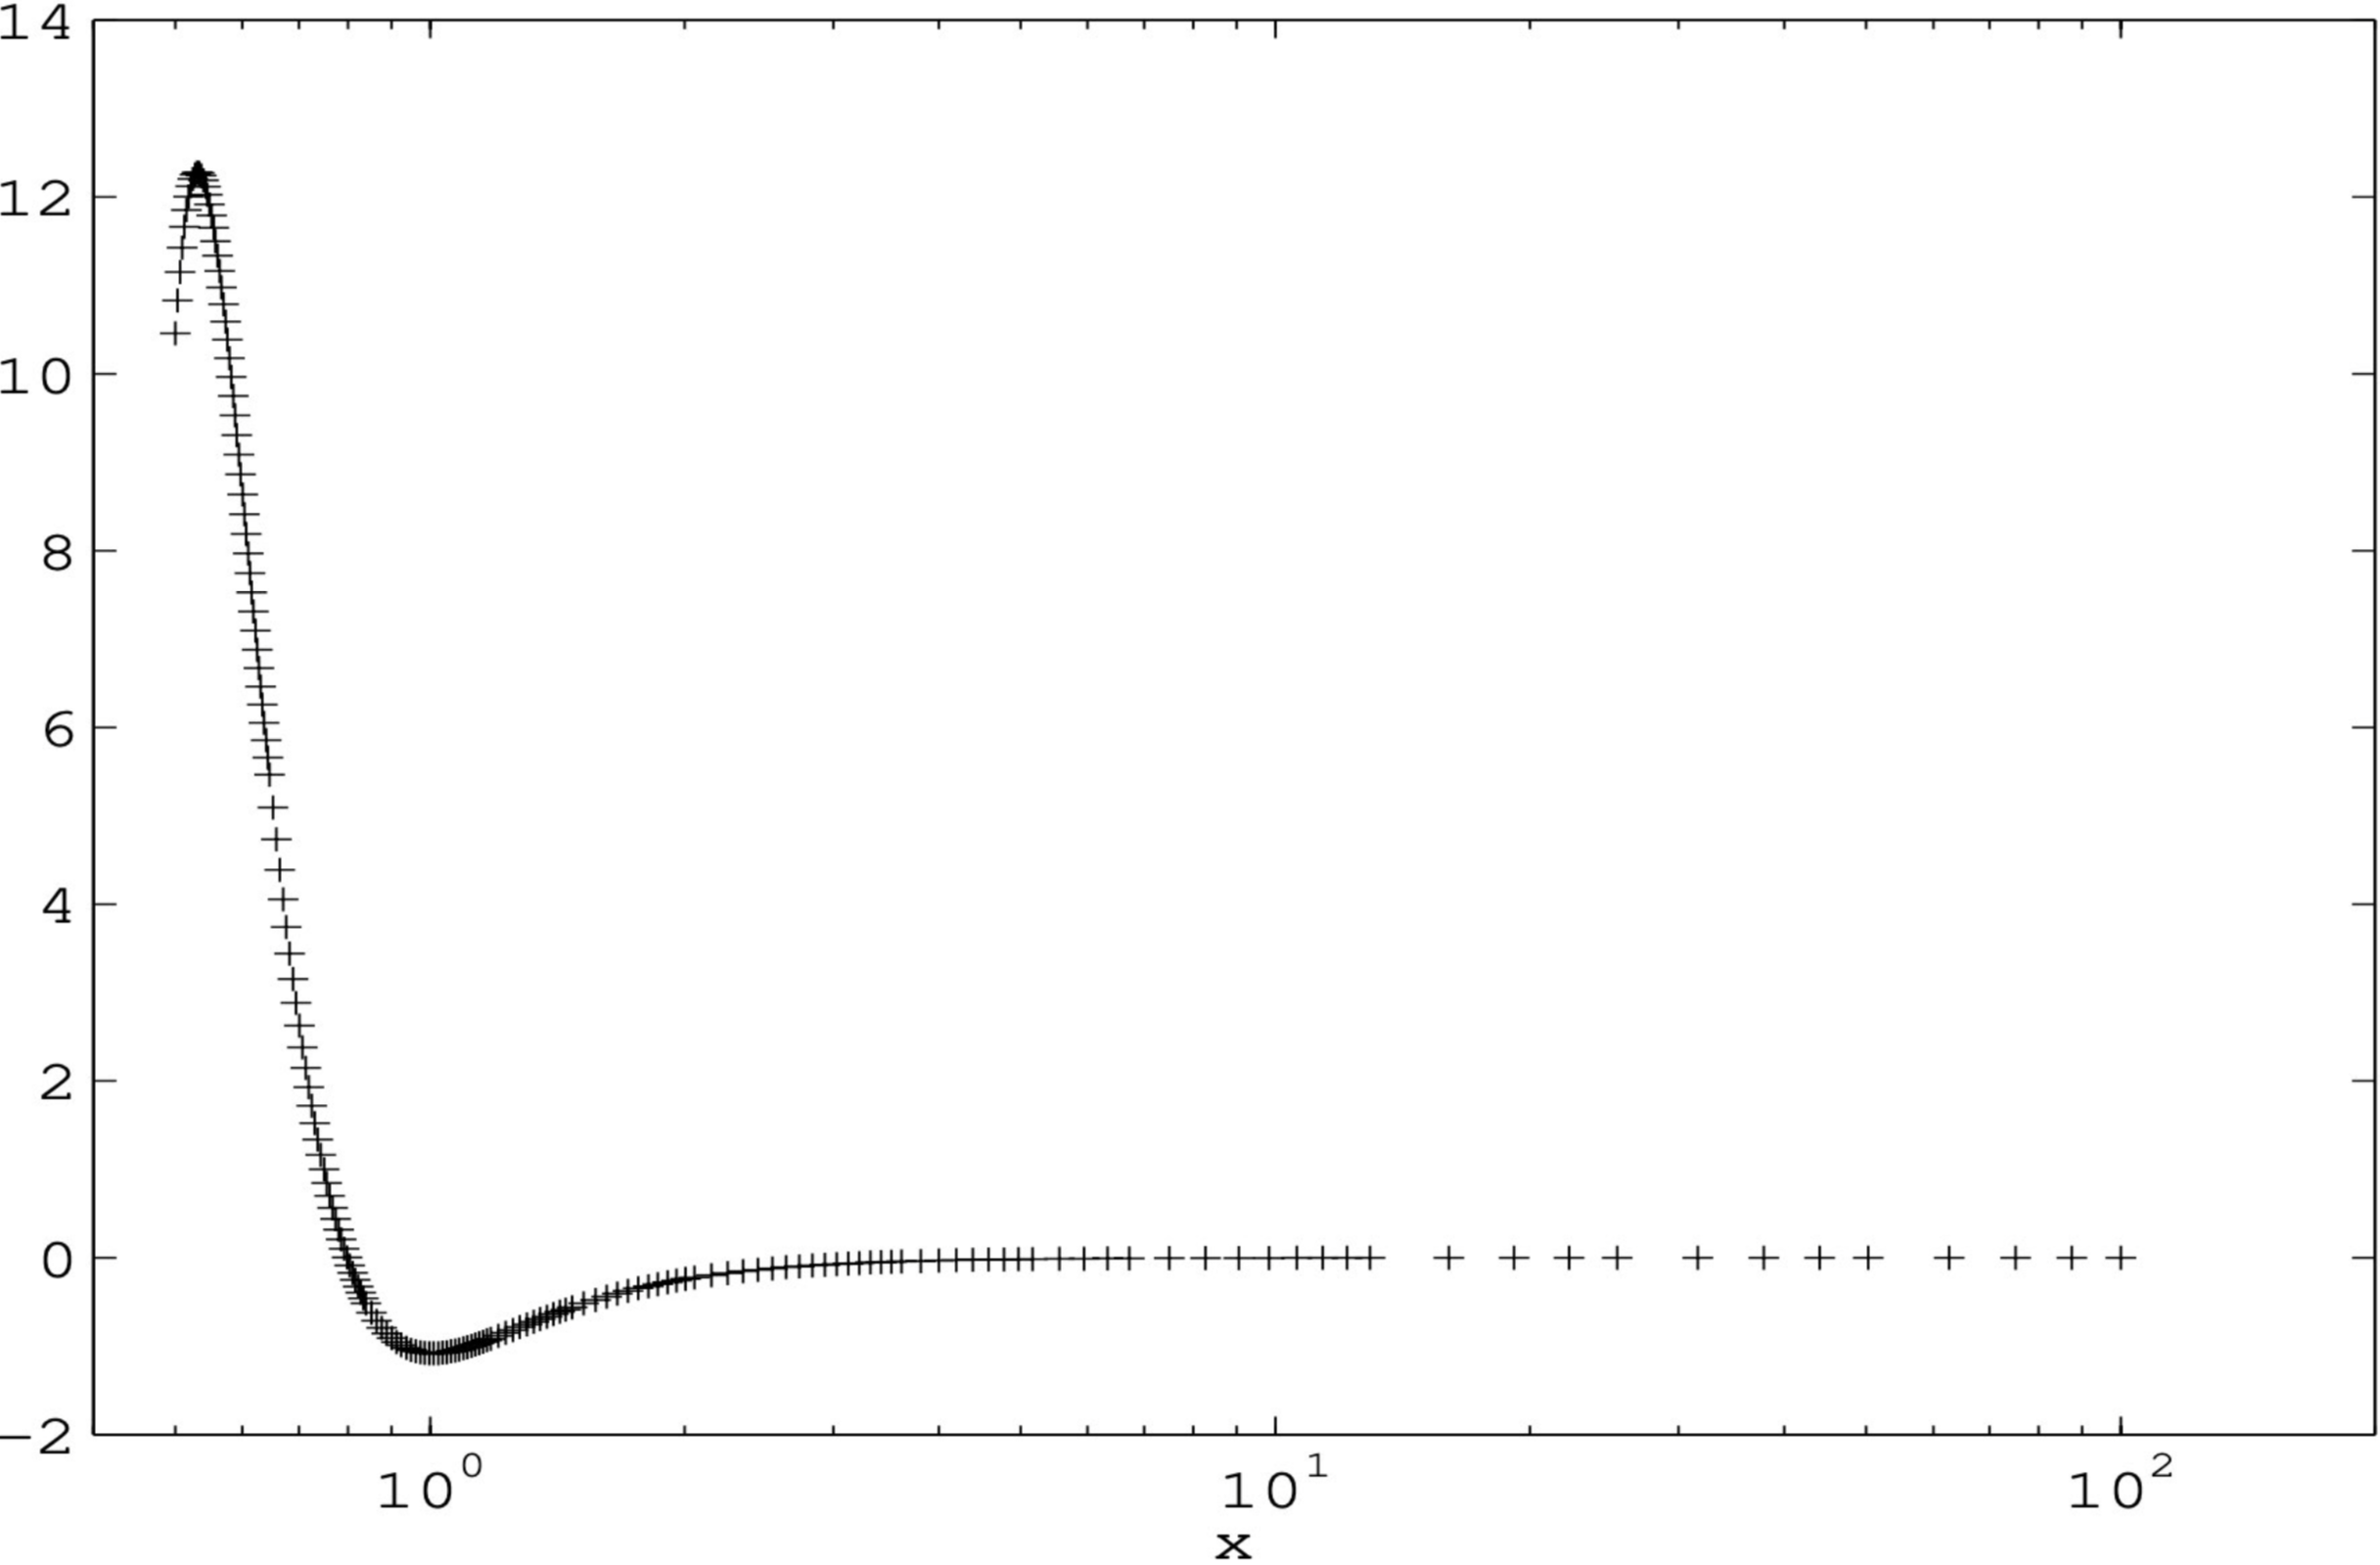
\includegraphics[width=0.5\textwidth]{immagini/simpsonAdatToll=10e-5.png}
    \caption{Simpson adattivo con $\boldsymbol{tol=10e-5}$.}\label{fig:simpsonAdatToll=10e-5}
\end{figure}

\begin{algorithm}\caption{Implementazione algoritmo adattivo dei trapezi.}
\label{alg:algAdattFormTrap}
    \begin{lstlisting}[style=Matlab-editor]
    function I2 = adaptrap(f, a, b, tol, fa, fb)
    %
    % Utilizzo:tab I2 = adaptrap(f, a, b, tol) [questa e' un'interfaccia utente, viene invocata la prima volta. fa e fb sono utilizzati per implementare la funzione ricorsivamente, quindi dalla seconda invocazione della function] [Nel caso della function che implementa la funzione Simpson e' necessario prevere 3 valutazioni funzionali, non come nelle implementazioni della formula dei trapezi, la quale richiede due valutazioni in input]
    %
    % Input:
    %   f - function handler funzione integranda;
    %   a,b - estremi intervallo di integrazione;
    %   tol - accuratezza richiesta.
    %
    % Output:
    %   I2 - approssimazione ottenuta.
    if nargin < 4 
        error('numero argomenti insufficienti')
    end
    if tol <= 0 
        error('tolleranza nulla o minore di 0')
    end 
    if nargin == 4
        fa = feval(f, a); fb = feval(f, b);
    end
    h = b - a;
    x1 = (a + b)/2;
    f1 = feval(f, x1); %valutazione funzionale nel punto medio
    I1 = (h/2)*(fa+fb); 
    I2 = (I1 + h*f1)/2; 
    e = abs(I2-I1)/3; %stima dell'errore
    if e > tol
        I2 = adaptrap(f, a, x1, tol/2, fa, f1)...
            + adaptrap(f, x1, b, tol/2, f1, fb); 
    end
    return
    \end{lstlisting}
\end{algorithm}


\section{Esercitazione capitoli 1 e 2}
\subsection{A.A. 2022/23}
\begin{enumerate}
	\item Approssimando $\pi = 3.14159265\hdots$ con $3.14$:
	\begin{itemize}
		\item qual è l’errore assoluto commesso?
		\item  qual è quello relativo?
	\end{itemize}
	(approssimare la risposta a due cifre significative).
	\item Come si definisce la precisione di macchina di un’aritmetica finita? Qual è il suo significato?
	\item Qual è la precisione di macchina della singola e doppia precisione IEEE? Dedurre il numero di cifre decimali approssimativamente disponibili per la mantissa.
	\item Cosa è il fenomeno della cancellazione numerica?
	\item Come si definisce l’ordine di convergenza di un metodo per la ricerca degli zeri di una funzione?
	\item Qual è il numero massimo di iterazioni che richiederà il metodo di bisezione per determinare la radice di una funzione assegnata con tolleranza (assoluta) $10^{-3}$, se l’intervallo di confidenza iniziale è $[33, 37]$?
	\item Derivare il metodo di Newton per la ricerca della radice di una funzione e dimostrare che esso converge quadraticamente a radici semplici.
	\item Calcolare il numero di condizionamento della radice nulla di
	\begin{equation*}
		f(x)=3e^x-2\cos{x}-1.
	\end{equation*}
	\item Definire la molteplicità di una radice. Calcolare la molteplicità della radice nulla di
	\begin{equation*}
		f(x)=e^{x^2}-1.
	\end{equation*}
	Perché il calcolo di una radice nulla è un problema malcondizionato?
	\item Scrivere una function Matlab che implementi efficientemente il metodo di Newton.
\end{enumerate}

\hrule

\paragraph{1.}\footnote{Slide 3 PDF 13.} $x = 3.14159265\hdots,\, \Tilde{x}=3.14\Rightarrow\begin{cases}
	|\Delta x|=|\Tilde{x}-x|=0.0015926\hdots\approx 1.6\times 10^{-3},\\
	|\xi_x|=\frac{|\Delta x|}{|x|}=\frac{1.6\times 10^{-3}}{3.1415\hdots}\approx 5\times 10^{-4}.
\end{cases}$

\paragraph{2.}\footnote{Slide 3 PDF 13.} La precisione di macchina di un'aritmetica finita rappresenta una maggiorazione \textbf{uniforme} dell'errore relativo di rappresentazione, per numeri rappresentati da numeri di macchina normalizzati. Se è utilizzata una base $b$, con $m$ cifre per la mantissa, essa vale: $u=\begin{cases}
	b^{1-m},\;\text{in caso di rappresentazione con troncamento};\\
	\frac{1}{2}b^{1-m},\;\text{in caso di rappresentazione con arrotondamento.}
\end{cases}$

\paragraph{3.}\footnote{Slide 4 PDF 13. Nella rappresentazione binaria le cifre sono normalizzate, tutto cambia se è denormalizzato. La prima cifra considerata 1 quindi non è memorizzata memorizzando con 23 bit 24. Stesso cosa vale per la precisione macchina in doppia precisione.} Nella precisione IEEE è utilizzata la rappresentazione in base 2 con arrotondamento alla 24-esima cifra binaria. Pertanto la precisione di macchina è
\begin{equation*}
	\boldsymbol{u=\frac{1}{2}\cdot 2^{1-24}=2^{-24}}\approx\frac{10^{-6}}{16}\approx\boldsymbol{0.7\cdot 10^{-7}},
\end{equation*}
ovvero, poco più di 7 cifre decimali significative.

\noindent Per la doppia precisione, l'unica differenza consiste nel numero di cifre binarie significative, sono 53. Pertanto, 
\begin{equation*}
	\boldsymbol{u=\frac{1}{2}\cdot 2^{1-53}=2^{-53}\approx 10^{-16}},
\end{equation*}
ovvero, circa 16 cifre decimali.

\paragraph{4.}\footnote{Slide 4 PDF 13.} La cancellazione numerica consiste nella perdita di cifre significative, nel risultato, derivante dalla somma di addendi quasi opposti. Ciò è dovuto al malcondizionamento di questa operazione. Dati $x$ e $y$ numeri da sommare, il numero di condizionamento della somma è rappresentato da $\kappa=\frac{|x|+|y|}{|x+y|}$, il quale non è limitato superiormente se $x\approx -y$. 

\paragraph{5.}\footnote{Slide 5 PDF 13.} Sia $x_{n+1}=\Phi(x_n),\; n=0,1,\hdots,$ denota un generico metodo iterativo per la ricerca di una radice $\overline{x}$ dell'equazione $f(x)=0$. Supposto che $x_n\rightarrow\overline{x}$, per $n\rightarrow\infty$ e con $e_n=|x_n-\overline{x}|$ il corrispondente errore al passo $n$. Il metodo converge con ordine $p\geq 1 $ alla radice, se $p$ è il più grande valore reale per cui 
\begin{equation*}
	\lim_{n\rightarrow\infty}\frac{e_{n+1}}{e_n^p}=c<\infty,
\end{equation*}
dove $c$ è la costante asintotica dell'errore. Per $n>>1\Rightarrow e_{n+1}\approx c\cdot e_n^p$.

\paragraph{6.}\footnote{Slide 6 PDF 13.} Il metodo di bisezione dimezza, ad ogni iterazione, l'ampiezza dell'intervallo di confidenza. Pertanto, l'approssimazione al passo $n$, avrà una accuratezza $2^{-n}(b-a)$, essendo $b-a$ l'ampiezza dell'intervallo iniziale. In questo caso $b-a=4$, per cui è ottenuto, imponendo $2^{2-n}\leq 10^{-3}$, il numero massimo di iterazioni. Dato che $10^{-3}\approx 2^{-10}$ è ottenuto quanto segue: $2^{2-n}\leq 2^{-10}\Rightarrow 2-n\leq -10\Rightarrow n\geq 12 \Rightarrow\boldsymbol{n=12}\, \left(= \lceil\log_2(37-34)-\log_2(10^{-3})\rceil\right)$.

\paragraph{7.}\footnote{Slide 7 PDF 13.} Il metodo di Newton è ottenuto ricercando, ad ogni passo, la radice della retta tangente al grafico della funzione nell'approssimazione corrente (come in Figura \ref{fig:approxNewtEs10}).

\begin{figure}
	\centering
	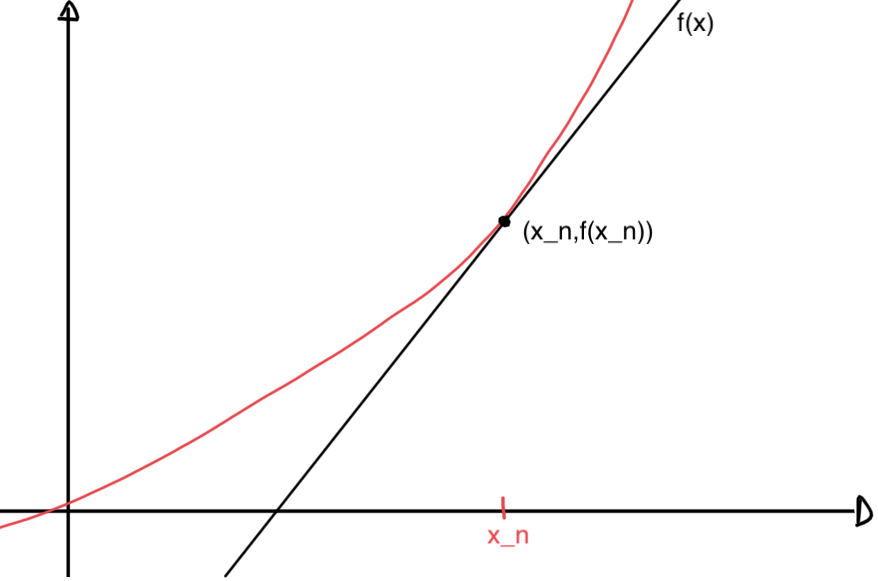
\includegraphics[width=0.5\textwidth]{immagini/approxNewtEs10.jpg}
	\caption{Approssimazione Esercizio 10.}\label{fig:approxNewtEs10}
\end{figure}

\noindent La retta tangente il grafico di $f(x)$ nel punto $(x_n, f(x_n))$ è $y-f(x_n)=f'(x_n)(x-x_n)$, essendo $f'(x_n)$ la derivata di $f(x).$ Ponendo $y=0$, è ricavata
\begin{equation*}
	x_{n+1}=x_n-\frac{f(x_n)}{f'(x_n)},\quad n=0,1,2,\hdots.
\end{equation*}

\noindent Dimostrare la convergenza quadratica ad una radice semplice di $ \overline{x}$ di $f(x)$ significa che $f'(x)\neq 0$, sotto ipotesi che $f\in C^{(2)}$ in un intorno di $\overline{x}$, per un opportuno intorno, per il Teorema della permanenza del segno, significa:
\begin{equation*}
	\begin{matrix}
		0&=&f(\overline{x})&=& f(x_n)+(\overline{x}-x_n)f'(x_n)+\frac{f''(\xi_n)}{2}(\overline{x}-x_n)^2&&\\
		&=&f'(x_n)\left(\boldsymbol{\frac{f(x_n)}{f'(x_n)}-x_n}+\overline{x}\right) + \frac{f''(\xi_n)}{2}(\overline{x}-x_n)^2&\overset{\footnotemark}{=}& f'(x_n)(x_{n+1}-\overline{x})+\frac{f''(\xi_n)}{2}(\overline{x}-x_n)^2\\
		&&&&\xi_n\in\underset{\footnotemark}{\uline{I(\overline{x}, x_n)}}
	\end{matrix}
\end{equation*}

\addtocounter{footnote}{-1}
\footnotetext{$\frac{f(x_n)}{f'(x_n)}-x_n$ è Newton al passo $n+1$, ovvero $x_{n+1}$.}

\stepcounter{footnote}
\footnotetext{Intervallo aperto nel quale gli estremi sono massimo e minimo. Se $x_n\rightarrow\overline{x}$ significa che anche $\xi_n\rightarrow\overline{x}$.}

\noindent Da questo segue che $f'(x_n)(\overline{x}-x_{n+1})=\frac{f''(\xi_n)}{2}(\overline{x}-x_n)^2.$ Ponendo $e_n=\overline{x}-x_n$ e dato che $f'(\overline{x})\neq 0$ è ottenuto ciò che segue: 
\begin{equation*}
	\frac{e_{n+1}}{e_n^2}=\frac{f''(\xi_n)}{2f'(x_n)}\longrightarrow\lim_{n\rightarrow\infty}\frac{|e_{n+1}|}{|e_n|^2}=\lim_{n\rightarrow\infty}\left|\frac{f''(\xi_n)}{2f'(x_n)}\right|=\left|\frac{f''(\overline{x})}{2f'(\overline{x})}\right|<\infty.
\end{equation*}

\paragraph{8.}\footnote{Slide 9 PDF 13.} Il numero di condizionamento di una radice è dato da $\boldsymbol{\frac{1}{|f'(\overline{x})|}}$, se $\overline{x}$ è la radice. In questo caso $f'(x)=3e^x+2\sin{(x)}\rightarrow f'(0)=3$. Pertanto, il numero di condizionamento della radice nulla di $f(x)$ vale $\boldsymbol{\frac{1}{3}}$

\paragraph{Osservazione sugli scritti:} Meglio scrivere ciò di cui siamo sicuri in termini di passaggi intermedi, altrimenti è meglio scrivere solo il risultato finale.

\paragraph{9.}\footnote{Slide 9 PDF 13.} La radice $\overline{x}$ di $f(x)=0$ ha molteplicità $m$ se:
$\begin{cases}
	f(\overline{x})=f'(\overline{x})=\hdots=f^{(\boldsymbol{m-1})}(\overline{x})=0,\\
	f^{(\boldsymbol m)}(\overline{x})\neq 0.
\end{cases}$

\noindent Se $\boldsymbol{m=1}$ la radice è \textbf{semplice}, se $\boldsymbol{m>1}$ la radice è \textbf{multipla}. La determinazione di una radice multipla è un problema malcondizionato, per il numero della radice, $\frac{1}{f'(\overline{x})}$, è infinito, essendo $f'(\overline{x})=0$. 

\noindent Data $f(x)=e^{x^2}-1\Rightarrow\boldsymbol{f(0)=0}$. Inoltre, $f'(x)=2xe^{x^2}\Rightarrow\boldsymbol{f'(0)=0}$ \footnote{Quindi, da qui, è possibile capire che la radice non è semplice.}. Ancora, $f''(x)=2e^{x^2}+4x^2e^{x^2}\Rightarrow\boldsymbol{f''(0)=2\neq 0}.$ Pertanto, la radice ha \textbf{molteplicità 2}.

\paragraph{10.} L'implementazione richiesta è nell'Algoritmo \ref{alg:polNewt}

\subsection{A.A. 2023/24}
\subsubsection{Esercitazione 10/01/24}
\begin{enumerate}
	\item Approssimando $e=2.71828\hdots$ con $2.72$
	\begin{itemize}
		\item qual è l'errore assoluto commesso?
		\item qual è l'errore relativo?
	\end{itemize}
	\item Come si definisce la precisione di macchina di un'aritmetica finita? Qual è il suo significato?
	\item Dimostrare che, se $h\approx 0$, allora
	\begin{equation*}
		\frac{f(x+h)-f(x-h)}{2h}=f'(x)+o(h^2).
	\end{equation*}
	\item Cos'è il fenomeno della cancellazione numerica?
	\item Come si definisce l'ordine di convergenza di un metodo per la ricerca degli zeri di una funzione?
	\item Qual è il numero di massimo di iterazioni richiesto dal metodo di bisezione per determinare la radice di una funzione di cui sia noto l'intervallo di confidenza iniziale $[33,41]$, con accuratezza di $10^{-3}$?
	\item Derivare il metodo di Newton per la ricerca della radice di una funzione, e dimostrare che converge quadraticamente a radici semplici.
	\item Calcolare il numero di condizionamento della radice nulla di $f(x)=3\cos x-2-e^x$.
	\item Definire la molteplicità di una radice. Calcolare la molteplicità della radice nulla di
	\begin{equation*}
		f(x)=x\cos x - \sin x + \frac{x^3}{3}.
	\end{equation*}
	Perché il calcolo di una radice multipla è malcondizionato?
\end{enumerate}

\hrule

\paragraph{1.} L'errore assoluto è dato, se $x=e$ e $\tilde x=2.72$, da:
\begin{equation*}
	\Delta x=\tilde x - x = 2.72 - 2.71828\hdots \approx 2\cdot 10^{-3}.
\end{equation*}
Il corrispondente errore relativo è dato da:
\begin{equation*}
	\varepsilon_x = \frac{\Delta x}{x} = \frac{2    \cdot10^{-3}}{2.71828}\approx 7\cdot 10^{-4}.
\end{equation*}

\paragraph{2.} \footnote{Da Teorema \ref{th:precisione_macchina_FL}.} Se si utilizza un'aritmetica finita in base $b$, con $m$ cifre per la mantissa, la corrispondente precisione di macchina è definita da:
\begin{equation*}
	u=
	\begin{cases}
		b^{1-m}, &\text{ in caso di troncamento},\\
		\frac{1}{2}b^{1-m}, &\text{ in caso di arrotondamento}.
	\end{cases}
\end{equation*}
Il suo significato è il seguente: dato $x\in\mathbb R$ e detto $fl(x)$ il corrispondente numero di macchina, se questo è normalizzato, allora la precisione macchina, maggiora uniformemente l'errore relativo di rappresentazione
\begin{equation*}
	\frac{|x-fl(x)|}{|x|}\leq u\quad (\text{se } x\neq 0).
\end{equation*}
$fl(x)$ è normalizzato se la prima cifra della mantissa è diversa da 0.

\paragraph{N.B.:} \textbf{È necessario conoscere la precisione macchina della singola e doppia precisione.}

\paragraph{3.}
\begin{itemize}
	\item $f(x+h)=f(x)+hf'(x)+\frac{h^2}{2}f''(x)+o(h^3)$,
	\item $f(x-h)=f(x)-hf'(x)+\frac{h^2}{2}f''(x)+o(h^3)$.
\end{itemize}
Sottraendo membro a membro, si ottiene:
\begin{equation*}
	f(x+h)-f(x-h)=2h\,f'(x)+o(h^3),
\end{equation*}
da cui, dividendo per $2h$, si ottiene
\begin{equation*}
	\frac{f(x+h)-f(x-h)}{2h}=f'(x)+o(h^2).
\end{equation*}

\paragraph{4.}\footnote{Vedere Sezione \ref{sssec:condizionamento_somma_algebrica}.} Questo fenomeno è la manifestazione del malcondizionamento della somma algebrica, in caso di addendi di segno discorde. Infatti, se $\tilde x_1 = x_1 (1+\varepsilon_1)$ e $\tilde x_2 = x_2 (1 + \varepsilon_2)$ sono gli addendi perturbati, allora $\tilde y = y (1 + \varepsilon_y)$ sarà il corrispondente risultato perturbato:
\begin{equation*}
	\begin{matrix}
		y &=& x_1 + x_2\\
		\tilde y &=& \tilde x_1 + \tilde x_2 &=& x_1(1+\varepsilon_1) + x_2 (1+\varepsilon_2) &=& \underbrace{x_1 + x_2}_{y} + x_1 \varepsilon_1 + x_2 \varepsilon_2.
	\end{matrix}
\end{equation*}
Da questo si ricava:
\begin{equation*}
	\boldsymbol{\varepsilon_y} = \frac{x_1\varepsilon_1+x_2\varepsilon_2}{x_1+x_2}= \boldsymbol{\frac{x_1\varepsilon_1+x_2\varepsilon_2}{y}},
\end{equation*}
da cui:
\begin{equation*}
	|\varepsilon_y|\leq \frac{|x_1|+|x_2|}{|x_1+x_2|} \cdot \max{\{|\varepsilon_1|,|\varepsilon_2|\}}.
\end{equation*}
Pertanto, il numero di condizionamento della somma algebrica è
\begin{equation*}
	\kappa=\frac{|x_1|+|x_2|}{|x_1+x_2|},
\end{equation*}
che non è limitato superiormente se $x_1$ e $x_2$ sono quasi opposti. In questo caso, il malcondizionamento del problema si manifesta, utilizzando un'aritmetica finita, nel fatto che, anche partendo da addendi con tutte le cifre significative corrette, si può ottenere un risultato con molte meno cifre significative corrette.
\paragraph{Nota:} È possibile fare un esempio di malcondizionamento di una somma algebrica.

\paragraph{5.} Se consideriamo un metodo iterativo per determinare una conveniente approssimazione dello zero di una funzione, sia esso $x^*$, allora, dette $x_1, x_2,\hdots, x_n$ le apporssimazioni generate, il metodo avrà ordine di convergenza $p$ se, detto $e_n=x_n-x^*$ l'errore al passo $n$, si ha che  $p$ è il più alto valore per cui
\begin{equation*}
	\lim_{n\rightarrow\infty}\frac{|e_{n+1}|}{|e_n|^p}=c<+\infty.
\end{equation*}
$c$ si dice costante asintotica dell'errore.
\paragraph{N.B.:} È necessario conoscere l'ordine di convergenza dei metodi studiati.

\paragraph{6. } Ricordiamo che il metodo di bisezione approssima la soluzione col punto medio dell'intervallo di confidenza corrente. Pertanto, al passo $i$-esimo, l'errore sarà maggiorato $2^{-1}$ per l'ampiezza dell'intervallo di confidenza iniziale. Nel nostro caso, $41-33=8=2^3$. Pertanto, richiedendo che
\begin{equation*}
	2^-1\cdot 2^3\leq 10^{-3}\approx 2^{-10},
\end{equation*}
si ottiene $2^{-i}\leq 2^{-13}$, ovvero $i=13$ passi.

\paragraph{7.} Il metodo di Newton si deriva ricercando, ad ogni iterazione, la radice dell'approssimazione lineare della funzione nel punto corrente. Se ci trociamo nel punto $x_1$, allora
\begin{equation*}
	f(x)\cong f(x_i)+(x-x_i)f'(x_i),
\end{equation*}
che è l'equazione della retta tangente al grafico di $f(x)$ in $(x_i, f(x_i))$.\\
Ricercando $x_{i+1}$ in modo tale che
\begin{equation*}
	f(x_i)+(x_{i+1}-x_i)f'(x_i)=0,
\end{equation*}
si ottiene:
\begin{equation*}
	x_{i+1}=x_i-\frac{f(x_i)}{f'(x_i)},\quad i=0,1,\hdots\, .
\end{equation*}
Per quanto riguarda la seconda parte, supponiamo $\boldsymbol{x_i\rightarrow\overline{x}},\, i\rightarrow +\infty$, radice semplice di $f(x)$. Pertanto, $\boldsymbol{f'(\overline{x})\neq 0}$. Si ottiene:
\begin{equation*}
	0=f(\overline{x})=f(x_i)+(\overline{x}-x_i)f'(x_i)+\frac{(\overline{x}-x_i)^2}{2}f''(\boldsymbol{\xi_i}),\quad \boldsymbol{\xi_i\in I(x_i,\overline{x})}.
\end{equation*}
Definendo $\boldsymbol{\overline{x}-x_i = e_i}$, l'errore al passo $i$, si ottiene, quindi:
\begin{equation*}
	\begin{matrix}
		0 &=& f(x_i)+(\overline(x)-x_i)f'(x_i)+\frac{(\overline{x}-x_i)^2}{2}f''(\xi_i) &=& \left[\overbrace{\frac{f(x_i)}{f'(x_i)}-x_i}^{-x_{i+i}} - \overline{x}\right]f'(x_i) + \frac{(\overline{x}-x_i)^2}{2} f''(\xi_i)\\
		&=& \underbrace{\left[\overline{x}-x_{i+1}\right]}_{e_{i+1}} f'(x_i) + \frac{(\overbrace{\overline{x}-x_i}^{e_i})^2}{2} f''(\xi_i) &=& e_{i+1} f'(x_i) + \frac{e_i^2}{2} f''(\xi_i).
	\end{matrix}
\end{equation*}
Pertanto,
\begin{equation*}
	\frac{|e_{i+1}|}{|e_i|^2}=\frac{1}{2}\frac{|f''(\xi_i)|}{|f'(\xi)|}\underset{i\rightarrow+\infty}{\longrightarrow}\frac{1}{2}\frac{|f''(\overline{x})|}{|f'(\overline{x})|},
\end{equation*}
che è finito, poiché $f'(\overline{x})\neq 0$.\\
Pertanto, si ha convergenza quadratica.

\paragraph{Suggerimento:} Riguardare la derivazione del metodo di accelerazione di Aitken.

\paragraph{8.} Se $\overline{x}$ è la radice di $f(x)$, il suo numero di condizionamento è definito da
\begin{equation*}
	\kappa = \frac{1}{|f'(\overline{x})|}.
\end{equation*}
Nel nostro caso,
\begin{equation*}
	f'(x)=-3\sin x - e^x
\end{equation*}
e, quindi, $|f'(0)|=1$.\\
Il numero di condizionamento della radice nulla è $\kappa=1$.

\paragraph{9.}\footnote{Dalla Definizione \ref{def:radice_molteplicita_m}.} Diremo che $\overline{x}$ è radice di molteplicità $m$ di $f(x)$ se
\begin{equation*}
	f(\overline{x})=f'(\overline{x})=f''(\overline{x})=\hdots=f^{(m-1)}(\overline{x})=0,\, f^{(m)}(\overline{x})\neq 0.
\end{equation*}
La radice $\overline{x}$ si dice semplice se $m=1$, multipla se $m>1$.
\begin{equation*}
	\begin{matrix}
		m=0 & f(x) = x\cdot\cos x-\sin x + \frac{x^3}{3} & \rightarrow & f(0)=0 ;\\
		m=1 & f'(x) = \cancel{\cos x} - x \sin x - \cancel{\cos x} + x^2 & \rightarrow & f'(0)=0 ;\\
		m=2 & f''(x) = -\sin x - \cos x + 2x & \rightarrow & f''(0)=0 ;\\
		m=3 & f'''(x) = -\cos x -\cos x + x\sin x  + 2 & \rightarrow & f'''(0)=0 ;\\
		m=4 & f^{(4)}(x) = 2\sin x + \sin x + x\cos x & \rightarrow & f^{(4)}(0)=0 ;\\
		m=5 & f^{(5)}(x) = 3\cos x + \cos x - x\sin x & \rightarrow & f^{(5)}(0)=4\neq 0 .
	\end{matrix}
\end{equation*}
Pertanto, la molteplicità della radice è $m=5$.\\
Il numero di condizionamento di $\overline{x}$, radice di $f$, è $\kappa = \frac{1}{|f'(\overline{x})|}$. Se la radice è multipla allora $f'(\overline{x})=0$ allora $\kappa=+\infty$.

\paragraph{10.} Ricordiamo che il metodo delle secanti è un metodo a 2 passi, definito dall'iterazione:
\begin{equation*}
	x_{i+1}=x_i-\frac{f(x_i)}{\frac{f(x_i)-f(x_{i-1})}{x_i-x_{i-1}}}=x_i-(x_i-x_{i-1})\cdot\frac{f(x_i)}{f(x_i)-f(x_{i-1})}=x_i-\frac{f(x_i)(x_i-x_{i-1})}{f(x_i)-f(x_{i-1})},\quad i=1,2,\hdots
\end{equation*}

Per l'implementazione vedere l'Algoritmo \ref{alg:metodo_secanti}.

\section{Esercitazione capitolo 3}
\subsection{A.A. 2022/23}
\begin{enumerate}
    \item  Scrivere una function Matlab che risolva efficientemente un sistema triangolare inferiore.
    \item Definire la fattorizzazione $LU$ di una matrice nonsingolare. Dimostrare che, se fattorizzabile, la fattorizzazione $LU$ di una matrice è unica.
    \item  Sotto quali condizioni esiste la fattorizzazione $LU$ di una matrice?
    \item Definire cosa si intende per matrice a diagonale dominante. Dimostrare che una matrice diagonale dominante è fattorizzabile $LU$.
    \item  Definire cosa si intende per matrice simmetrica e definita positiva (sdp). Dimostrare che una matrice sdp è fattorizzabile $LU$ .
    \item Dimostrare che una matrice simmetrica e definita positiva è fattorizzabile nella forma $LDL^T$, con $L$ triangolare inferiore a diagonale unitaria, e $D$ matrice diagonale.
    \item  Definire cosa si intende per norma indotta su matrice. Dare qualche esempio di tali norme.
    \item  Definire cosa è il numero di condizionamento di una matrice. Spiegarne il significato.
    \item Definire la soluzione nel senso dei minimi quadrati di un sistema lineare sovra-determinato a rango pieno. Dimostrarne l’esistenza ed unicità.
    \item Calcolare la matrice elementare di Householder $H$ relativa al vettore: 
    \begin{equation*}
       \boldsymbol z = \begin{pmatrix}
        -1\\
        2\\
        -2
    \end{pmatrix}.
    \end{equation*}
    Quanto vale il prodotto $H\boldsymbol z$?
    \item Definire il metodo di Newton per sistemi nonlineari, e dettagliarne l’implementazione.
\end{enumerate}

\paragraph{1.}\footnote{Slide 3 PDF 14.} La function è implementata nell'Algoritmo \ref{alg:trilow}.

\begin{algorithm}
\caption{Implementazione efficiente risolutore sistema triangolare inferiore.}\label{alg:trilow}
    \begin{lstlisting}[style=Matlab-editor]
    function y = trilow(L, b)
    %   
    %   y = trilow(L, b)
    %
    %   Risolve un sistema triangolare inferiore
    %
    % Input:
    %   L   -  matrice dei coefficienti;
    %   b  -   termine noto;
    %   
    % Output:
    %   y   -   vettore soluzione.
    %
    % Le prossime tre righe sono controlli iniziali.
    [m,n] = size(L);
    if m ~= n, error('Matrice non quadrata'), end
    if n~= length(b), error('Termine noto non consistente'), end

    y=b(:); %trasformazione di b in vettore colonna
    
    for i = 1 : n
        if L(i,i) == 0, error('Matrice singolare'), end
        y(i) = y(i)/L(i,i);
        y(i+1:n) = y(i+1:n) - L(i+1:n, i)*y(i):
    end
    return
    \end{lstlisting}
\end{algorithm}

\paragraph{2.}\footnote{Slide 3 PDF 14.} Sia $A\in\mathbb R^{n\times n},\, \det(A).$

\noindent (Risposta alla prima parte di domanda:) $A$ è fattorizzabile $LU$, se $A=LU$, con:
\begin{itemize}
    \item $L$ triangolare inferiore a diagonale unitaria:
    \item $U$ triangolare superiore.
\end{itemize}

\noindent (Risposta alla seconda parte) Unicità della fattorizzazione: È necessario dimostrare che se $A=L_1U_1$ è un'ulteriore fattorizzazione $LU$ di $A$, allora $L=L_1,\, U=U_1.$ Infatti:
\begin{equation*}
    0\neq\det(A)=\det(LU)=\underbrace{\det(L)}_{\footnotemark}\det(U)=\det(U).
\end{equation*}
\footnotetext{Uguale ad 1 perché a diagonale unitaria 1.}

\noindent Pertanto, da $LU=L_1U_1$, segue che, moltiplicando a destra per $U^{-1},\, L=L_1U_1U^{-1}.$ Da questa, moltiplicando a sinistra per $L_1^{-1},$ segue che:
\begin{equation}\label{eq:LL=UU}
    L_1^{-1}L=U_1U^{-1}.
\end{equation}

\noindent È possibile osservare ciò che segue:
\begin{itemize}
    \item $L_1^{-1}$ è una matrice triangolare inferiore a diagonale unitaria;
    \item  $U^{-1}$ è una matrice triangolare superiore.
\end{itemize}

\noindent Quindi $L_1^{-1}L$ è una matrice triangolare inferiore a diagonale unitaria e $U_1U^{-1}$ è una matrice triangolare superiore. Pertanto, le due matrici in (\ref{eq:LL=UU}) sono diagonali. Poichè la diagonale di $L_1^{-1}L$ è unitaria, questa è la matrice indentità. Dalle uguaglianze allora 
\begin{itemize}
    \item $L_1^{-1}L=I$,
    \item $U_1U^{-1}=I$,
\end{itemize}
segue che $L=L_1\wedge U_1=U$, ovvero la fattorizzazione $LU$ è unica. \qed

\paragraph{IMPORTANTE:} I passaggi come quelli sopra è necessario che siano il piu' dettagliati possibile affinché Luigi sappia che abbiamo studiato.

\paragraph{3.} Sia $A\in\mathbb R^{n\times n}, \det(A)\neq 0.$ Denotando con $A_k$ la sottomatrice principale di ordine $k$ di $A$, allora:
\begin{equation*}
    A=LU\iff\forall k=1,\hdots, n\, :\,\det(A_k)\neq 0.
\end{equation*}
Questa ultima riga non è sufficiente, è necessario specificare $A\in\mathbb R^{n\times n}.$

\paragraph{4.}\footnote{Slide 6 PDF 14.} Sia $\boldsymbol{A\in\mathbb R^{n\times n}}$. Allora $A=(a_{ij})$ è:
\begin{itemize}
    \item \textbf{diagonale dominante per righe}, se
    \begin{equation}\label{eq:ddRighe}
        |a_{ii}|>\sum_{j\neq i, j=1}^n|a_{ij}|,\quad\forall i=1,\hdots,n;
    \end{equation}
    \item \textbf{diagonale dominante per colonne}, se $|a_{jj}|>\sum_{i\neq j, i=1}^n |a_{ij}|,\;\forall j=1,\hdots,n.$
\end{itemize}
Valgono le seguenti proprietà:
\begin{itemize}
    \item[\textbf{P1)}] $A$ è d.d. per righe $\iff A^T$ è d.d. per colonne;
    \item[\textbf{P2)}] Se $A$ è d.d. per righe (o colonne), allora, detta $A_k$ la sottomatrice principale di ordine $k$ di $A$, essa sarà d.d. per righe (o colonne). (Dimostrazione:) Infatti, dato un generico $k\in\{1,\hdots,n\},$ risulterà che dalla (\ref{eq:ddRighe}) segue che $\forall i=1\hdots,k:$
    \begin{equation*}
         |a_{ii}|>\sum_{j\neq i, j=1}^n|a_{ij}|\geq \sum_{j\neq i, j=1}^k|a_{ij}|,
    \end{equation*}
    ovvero, $A_k$ è diagonale d.d. per righe. Analogamente per $A$ d.d. per colonne.\qed
    \item[\textbf{P3)}] Se $A$ è d.d. per righe (o per colonne), allora $A$ è non singolare. Infatti, se $A$ fosse singolare, esisterebbe $\uline{x}\in\mathbb R^n,\, x\neq 0\,:\, A\uline{x}=\uline 0$. Questa equazione vale per ogni multiplo di $\uline x$ quindi è possibile normalizzare $\uline x$ in modo che $x_k=\underset{i=1,\hdots,n}{\max}|x_i|=1$. Pertanto, la $k$-esima equazione di $A\uline x=\uline 0$ diviene: $\sum_{j=1}^na_{kj}x_j=0.$ Da questo segue che $a_{kk}\,x_k=-\sum_{j=1,j\neq k}^n a_{kj}x_j.$ Pertanto:
    \begin{equation*}
        |a_{kk}|=|a_{kk}x_k|=\left|\sum_{j=1,j\neq k}^n a_{kj}x_j\right|\leq\sum_{j=1,j\neq k}^n |a_{kj}|\cdot\underbrace{|x_j|}_{\leq 1}\leq\sum_{j=1,j\neq k}^n |a_{kj}|,
    \end{equation*}
    il che contradice l'ipotesi d.d. per righe sulla riga $k$. Se A è d.d. per colonne, il tutto è riapplicato a $A^T$, che sarà d.d. per righe (per \textbf{P1)}).
\end{itemize}

\noindent Dalle proprietà \textbf{P2)} e \textbf{P3)}, segue che:
\begin{itemize}
    \item $A$ è d.d. per righe (o colonne) $\iff\forall k=1,\hdots,n;$
    \item $A_k$ è d.d. per righe (o colonne) $\iff\forall k=1,\hdots,n;$
    \item $\det(A_k)\neq 0\iff A$ è fattorizzabile $LU.$
\end{itemize}

\paragraph{5.}\footnote{Slide 9 PDF 14.} Sia $A\in\mathbb R^{n\times n}.$ A è simmetrica e definita positiva (sdp) se:
\begin{itemize}
    \item $A=A^T$ ($A$ è simmetrica);
    \item $\forall \uline x\in\mathbb R^n\backslash\{\uline 0\}\,:\, \uline x^T A \uline x > 0$ ($A$ è definita positiva).
\end{itemize}
Per dimostrare che, se $A$ è sdp, allora $A=LU$, sarà dimostrato che:
\begin{enumerate}
    \item $\forall k=1,\hdots, n$, $A_k$, detta sottomatrice principale di $A$ di ordine $k$, è sdp;
    \item $A$ sdp $\Rightarrow A$ è nonsingolare.
\end{enumerate}

\noindent Riguardo la 2), se $A$ non fosse singolare, allora $\exists\,\uline x\in\mathbb R^n\backslash\{\uline 0\}\, : \, A\uline x=\uline 0\Rightarrow\uline x^T A \uline x = 0,$ contraddicendo la definita positiva di A.
Pertanto, $A$ è nonsingolare.

\noindent Riguardo la 1): 
\begin{equation}\label{eq:ACompSimm}
\forall k=1,\hdots,n:\; 
A=\left[\begin{array}{c|c}
       A_k & B\\
       \hline
       C& D
    \end{array}
    \right],\text{ con } D\in\mathbb R^{(n-k)\times (n-k)}.    
\end{equation}
Dalla simmetria di $A$, segue che 
$A^T=\left[
\begin{array}{c|c}
    A_k & C^T\\
    \hline
    B^T & D^T
\end{array}
\right]=A.$ Uguagliando i blocchi omologhi allora:
\begin{equation*}
    A_k=A_k^T,\; B=C^T,\; D=D^T\;\rightarrow A_k \text{ è simmetrica.}
\end{equation*}

\noindent Rimane da dimostrare che, $\forall \uline y\in\mathbb R^k\backslash\{\uline 0\}\,:\, \uline y^TA_k\uline y > 0.$ A questo fine, assegnato un generico $\uline y\in\mathbb R^k\backslash\{\uline 0\}$, è considerato il vettore $\uline x=
\begin{pmatrix}
    \uline y\\
    \uline 0
\end{pmatrix}\in\mathbb R^n$. Chiaramente $\uline x\neq 0$. Dato che $A$ è sdp allora da (\ref{eq:ACompSimm}) segue che:
\begin{equation*}
    0<\uline x^T A \uline x = (\uline y^T\; \uline 0^T)\,\left[\begin{array}{c|c}
       A_k & B\\
       \hline
       C& D
    \end{array}
    \right]
    \begin{pmatrix}
        \uline y\\
        \uline 0
    \end{pmatrix} = 
    (\uline y^T\; \uline 0^T)
    \begin{bmatrix}
        A_k \uline y\\
        C \uline y
    \end{bmatrix} = \uline y^T A_k \uline y.
\end{equation*}\qed

\paragraph{6.}\footnote{Slide 11 PDF 14.}
È noto che, se $A$ è sdp, allora $A=LU$ ed è noto che la fattorizzazione $LU$ è unica. Pertanto, osservando il fattore $U$ può essere scritto come $D\widehat{U}$, con $D$ diagonale ed $\widehat{U}$ triangolare superiore a diagonale unitaria, segue che $A=LU=LD\widehat{U}$. Essendo $A=A^T\Rightarrow A=LD\widehat{U}=(LD\widehat{U})^T=A^T.$ Segue che $LD\widehat{U}=\widehat{U}^TDL^T.$

\noindent Essendo:
\begin{itemize}
    \item $\widehat{U}^T$ triangolare inferiore a diagonale unitaria,
    \item $DL^T$ triangolare superiore,
\end{itemize}
per l'unicità della fattorizzazione $LU$ segue che $L=\widehat{U}^T$. Da questo è possibile concludere che $A=LDL^T.$\qed

\paragraph{7.}\footnote{Slide 12 PDF 14.} Sia $||\cdot||$ una norma assegnata su vettore. È definito, data $A\in\mathbb R^{m\times n}$, la sua norma indotta dalla norma su vettore considerata: $||A||=\underset{\uline x\in\mathbb R^n, ||x||=1}{\max}||A\uline x||$.

\begin{remark}
    $||A\uline x||$ è la norma di un vettore di $\mathbb R^m.$
\end{remark}

\noindent Alcuni esempi: se $A=(a_{ij})\in\mathbb R^{m\times n},$ allora:
\begin{itemize}
    \item $||A||_1=\underset{j=1,\hdots,n}{\max}\sum_{i=1}^m|a_{ij}|;$
    \item $||A||_\infty=\underset{i=1,\hdots,m}{\max}\sum_{j=1}^n|a_{ij}|.$
\end{itemize}

\paragraph{8.}\footnote{Slide 12 PDF 14.} Sia $A\in\mathbb R^{n\times n},\;\det(A).$ Il suo numero di condizione, assegnato ad una generica norma indotta da una corrispondente norma su matrice, è definito come $\kappa(A)=||A||\cdot||A^{-1}||.$ Questo misura il condizionamento del sistema lineare $A\uline x= \uline b.$ Infatti, considerando perturbazioni $\Delta A$ e $\Delta\uline b$ su $A$ e $\uline b$, rispetivamente, è ottenuto $(A+\Delta A)(\uline x+\Delta\uline x)= \uline b+\Delta\uline b,$ con $\Delta\uline x$ perturbazione sul risultato. Vale che:
\begin{equation*}
    \frac{||\Delta\uline x||}{||\uline x||}\leq\kappa(A)\left(\frac{||\Delta\uline b||}{||\uline b||}+\frac{||\Delta A||}{||A||}\right)\qed
\end{equation*}

\paragraph{9.}\footnote{Slide 13 PDF 14.} Sia $A\in\mathbb R^{m\times n},$ con $m>n=rank(A).$ È definita \textbf{soluzione nel senso dei minimi quadrati} del sistema lineare $\boldsymbol{A\uline x=\uline b},$ il vettore $\boldsymbol{\uline x}$ \textbf{che minimizza la norma euclidea (al quadrato) del corrispondente vettore residue} $\boldsymbol{\uline r=A\uline x-\uline b}.$ \footnote{Necessario specificare la parte in grassetto affinché la risposta sia corretta.}

\noindent Il motivo della scelta della norma euclidea è dovuto al fatto che questa è invariante per moltiplicazione del vettore in argomento per una matrice ortogonale $Q$:
\begin{equation*}
    ||Q\uline v||_2^2=(Q\uline v)^T(Q\uline v)=\uline v^T \underbrace{Q^TQ}_{\footnotemark}=\uline v^T\uline v=||\uline V||_2^2.
\end{equation*}\footnotetext{Uguale ad $I$ perché $Q$ è ortogonale.}
La soluzione ai minimi quadrati di $A\uline x=\uline b$ è ottenuta osservando che, se $A\in\mathbb{m\times n},\; m>n=rank(A)$, allora esistono:
\begin{itemize}
    \item $Q\in\mathbb R^{m\times m},\; Q$ ortogonale ;
    \item $\widehat{R}\in\mathbb R^{n\times n},\;\widehat{R}$ triangolare superiore e nonsingolare,
\end{itemize}
tali che.: $A=QR,$ con $R=\begin{pmatrix}
    \widehat{R}\\
    0
\end{pmatrix}\in\mathbb R^{m\times n}.$ Per minimizzare:
\begin{equation*}
    \begin{matrix}
        ||\uline r||_2^2&=&||A\uline x-\uline b||_2^2&=&||QR\uline x-\uline b||_2^2 &=& ||Q(R\uline x - Q^T\uline b)||_2^2&\overset{\footnotemark}{=}&||R\uline x-\uline g||_2^2\\
        &\overset{\footnotemark}{=}&
        \Biggl|\Biggl|\begin{bmatrix}
            \widehat{R}\\
            0
        \end{bmatrix}\uline x
        - \begin{bmatrix}
            \uline g_1\\
            \uline g_2
        \end{bmatrix}\Biggl|\Biggl|_2^2&=&\Biggl|\Biggl|\begin{bmatrix}
            \widehat{R}\uline x -\uline g_1\\
            -\uline g_1
        \end{bmatrix}\Biggl|\Biggl|_2^2 &=& \left|\left|\widehat{R}\uline x - \uline g_1\right|\right|_2^2 + \left|\left|\uline g_2\right|\right|_2^2 &=& \left|\left|\uline g_2\right|\right|_2^2\\
        &&&&&&&=& \min!
    \end{matrix}
\end{equation*}

\addtocounter{footnote}{-1}
\footnotetext{Ponendo $\uline g=Q^T\uline b$ e sfruttando l'invarianza di $||\cdot||_2$.}

\stepcounter{footnote}
\footnotetext{$\uline g_1\in\mathbb R^n$.}

\noindent Scegliendo $\uline{x}$ come soluzione del sistema lineare $\widehat{R}\,\uline x=\uline g_1$, che esiste, ed è unica, essendo $\widehat{R}$ non singolare.

\paragraph{10.}\footnote{Slide 15 PDF 14.} È noto che $H\boldsymbol{\uline z}=\alpha\uline e_1\in\mathbb R^3, $ con $\alpha=\pm\left|\left|\uline z\right|\right|_2=\pm 3.$ La matrice $H$ è nella forma
\begin{equation*}
    H=I-\frac{2}{\uline v^T\uline v}\uline v\uline v^T,
\end{equation*}
con
\begin{equation*}
    \uline v=\uline z-\alpha \uline e_1=
    \begin{bmatrix}
        -1-\alpha\\
        2\\
        -2
    \end{bmatrix}=
    \begin{bmatrix}
        -1-3\\
        2\\
        -2
    \end{bmatrix}
\end{equation*}
avendo scelto \textbf{$\boldsymbol{\alpha=3}$, in modo che la prima componente di $\boldsymbol{\uline v}$ sia ottenuta sommando quantità concordi.} Segue che $\boldsymbol{H\uline z= 3\uline e_1}$. Il vettore di Householder è $\uline v=\begin{bmatrix}
    -4\\
    2\\
    -2
\end{bmatrix},$ dal quale è ottenuto che
\begin{equation*}
    H=I-\frac{2}{\uline v^T\uline v}\uline v\uline v^T=I-\frac{2}{24}\uline v \uline v^T=I-\frac{1}{12}\uline v\, \uline v^T.
\end{equation*}

\paragraph{11.}\footnote{Slide 17 PDF 14.} Sia $f\,:\,\mathbb R^m\rightarrow\mathbb R^m,$ è definito il metodo di Newton per risolvere $f(\uline x)=\uline 0$ fondamentalmente dall'iterazione seguente:
\begin{equation}\label{eq:passoFondamNewt}
    \uline x_{n+1}=\uline x_n - J_f(\uline x_n)^{-1}f(\uline x_n),\; n=0,1\hdots
\end{equation}
essendo $J_f(\uline x_n)$ la matrice Jacobiana di $f(\uline x)$ calcolata in $\uline x_n$. Nella pratica (\ref{eq:passoFondamNewt}) è implementata con l'obbiettivo di risolvere il sistema lineare $J_f(\uline x_n)\Delta \uline x_n=-f(\uline x_n)$ aggiornando $\uline x_{n+1}=\uline x_n+\Delta\uline x_n,\, n=0,1,\hdots\boldsymbol .$ Pertanto, il costo per iterazione è il seguente:
\begin{enumerate}
    \item 1 valutazione di $J_f$ e la sua fattorizzazione;
    \item 1 valutazione di $f$ e soluzione per i fattori di $J_f$;
    \item 1 axpy per aggiornare l'approssimazione corrente.
\end{enumerate}
Come criterio d'arresto è possibile utlizzare il seguente:
\begin{equation*}
    ||\Delta\uline x_n./(1+|\uline x|)||\leq tol, 
\end{equation*}
per una tolleranza $tol$ specificata.

\section{Esercitazione capitoli 4 e 5}
\subsection{A.A. 2022/23}
\begin{enumerate}
    \item  Formulare il problema dell'interpolazione polinomiale e dimostrare l'esistenza ed unicità del polinomio interpolante.
    \item Scrivere la forma di Lagrange del polinomio interpolante le coppie di dati (0, 1), (2, 3), (3, 7).
    \item Determinare la forma di Newton del polinomio interpolante i dati (0, 3), (2, 4), (3, 5). Sapendo che la derivata terza della funzione interpolanda ha norma minore o uguale a 5, dare una stima dell'errore di interpolazione nel punto $x = 4$.
    \item Derivare l'espressione dell'errore nell'interpolazione polinomiale.
    \item Costruire il polinomio di Hermite interpolante i dati,nella forma $(x_i, f_i , f'_i)$, (0, 1, 7) e (3, 4, -8).
    \item Definire la costante di Lebesgue, e spiegarne esaurientemente il significato nell'ambito dell'interpolazione polinomiale.
    \item Definire le ascisse di Chebyshev, e spiegarne il significato nell'ambito dell'interpolazione polinomiale.
    \item  Scrivere una \textit{function} Matlab che calcoli le ascisse di Chebyshev per costruire il polinomio interpolante di grado $n$ su un generico intervallo $[a, b]$.
    \item Cosa è il polinomio di migliore approssimazione di una funzione, e come questo è collegato all'errore nell'interpolazione polinomiale?
    \item Definire i polinomi di Chebyshev di prima specie, ed i corrispondenti polinomi monici. Qual è la caratteristica saliente di questi ultimi?
    \item Definire una funzione \textit{spline} di grado $m$ su una partizione $\Delta$ assegnata.
    \item Qual è l'unica funzione \textit{spline} univocamente determinata dalle condizionidi interpolazione sui nodi della partizione assegnata? Scriverne esplicitamente l'espressione.
    \item  Quante condizioni (indipendenti tra loro) servono per individuare univocamente una funzione \textit{spline}?
    \item Qual è l'unica funzione spline univocamente determinata dalle condizioni di interpolazione sui nodi della partizione assegnata? Scriverne esplicita- mente l'espressione.
    \item Quante condizioni servono per determinare univocamente una spline cu- bica interpolante? Cosa si intende per spline cubica interpolante naturale (completa/periodica/not-a-knot)?
    \item Scrivere una function Matlab che risolva efficientemente un sistema di equazioni tridiagonale (supporre che la matrice sia fattorizzabile $LU$).
    \item Definire il polinomio approssimante ai minimi quadrati. Sotto quali condizioni esso esiste ed è unico?
    \item Scrivere il problema algebrico che definisce il polinomio di approssimazione ai minimi quadrati di grado 2, per le coppie di dati (1,2), (1,2.1) (2,3), (3,4), (3,3) (4,5).
    \item Studiare il problema del condizionamento di un integrale definito.
    \item Derivare le formule di quadratura di Newton-Cotes.
    \item Calcolare $\int_0^\pi\cos{(x)}dx$ e la sua approssimazione con la formula dei trapezi e quella di Simpson, dettagliando i passaggi.
    \item Qual è l'espressione dell'errore della formula di Newton-Cotes di grado $k$? Quale quella della formula composita, supponendo che n sia multiplo di $k$?
    \item Come è possibile ottenere una stima dell'errore per la formula di Newton- Cotes di grado $k$, usata con n multiplo pari di $k$?
    \item Scrivere una function Matlab che calcoli efficientemente l'approssimazione di un integrale definito mediante la formula dei trapezi composita. Supporre che la function della funzione integranda accetti input vettoriali.
\end{enumerate}

\paragraph{2.}
\begin{equation*}
    p(x)=\sum_{i=0}^n f_iL_{in}(x),\quad L_{in}(x)=\prod_{j=0,\, j\neq i}^n\frac{x-x_j}{x_i-x_j},\quad i=0,\hdots,\, n.
\end{equation*}
Nel nostro caso:
$\begin{cases}
    n=2,\\
    x_0=0,\, x_1=2,\, x_2 = 3,\\
    f_0 = 1,\, f_1=3,\, f_2=7.
\end{cases}$

\noindent Pertanto:
\begin{equation*}
    p(x) = 1\cdot L_{02}(x)+3\cdot L_{12}(x) + 7\cdot L_{22}(x),
\end{equation*}
con
\begin{equation*}
    \begin{matrix}
        L_{02}(x) &=& \frac{(x-2)(x-3)}{(0-2)(0-3)} &=& \frac{(x-2)(x-3)}{6};\\
        L_{12}(x) &=& \frac{(x-0)(x-3)}{(2-0)(2-3)} &=& -\frac{1}{2}x(x-3);\\
        L_{22}(x) &=& \frac{(x-0)(x-2)}{(3-0)(3-2)} &=& \frac{x(x-2)}{3}.
    \end{matrix}
\end{equation*}

\noindent È possibile che inserisca un esercizio trabocchetto del tipo: calcolare polinomio interpolante, una funzione (polinomio) di grado 3, fornendo 18 coppie di punti. Questo significa che è ricercato il polinomio di grado al più 17. È chiaro che con il calcolo della funzione, questo sarà di una funzione minimale.

\paragraph{3.} In genere, si ha che
\begin{equation*}
    p(x) = \sum_{i=0}^n f[x_0,\hdots,\, x_i]\,\omega_i(x),
\end{equation*}
dove $f[x_0,\hdots, x_i]$ è la differenza divisa di $f$ sulle ascisse in argomento, e
\begin{equation*}
    \underset{\footnotemark}{w_i(x)}=\prod_{k=0}^{i-1}(x-x_k),\, i=0,\hdots, n.
\end{equation*}

\noindent Nel nostro caso:
$\begin{cases}
    n=2,\\
    x_0=0,\, x_1=2,\, x_2 = 3,\\
    f_0 = 3,\, f_1=4,\, f_2=5.
\end{cases}$

\noindent Pertanto:
\begin{itemize}
    \item[a)] $w_0(x)\equiv 1,\quad w_1(x)=x,\, w_2(x)=x(x-2),$
    \item[b)]
    \begin{tabular}{c|ccc}
         & 0 & 1 & 2 \\
         \hline
        $x_0=0$ & $\boldsymbol{f[x_0]=3}$\\
        $x_1=2$ & $f[x_1]=4$ & $\boldsymbol{f[x_0, x_1]=\frac{1}{2}}$\\
        $x_2=3$ & $f[x_2]=5$ & $f[x_1, x_2]=1$ & $\boldsymbol{f[x_0, x_1, x_2]=\frac{1}{6}}$
    \end{tabular}
    
    \noindent Concludiamo che:
    \begin{equation*}
        p(x)=3+\frac{1}{2}x+\frac{1}{6}x(x-2).\quad \text{[Fine prima parte del quesito]}
    \end{equation*}
\end{itemize}

\noindent [Risposta alla seconda parte del quesito:] Sappiamo che l'errore di interpolazione è dato da:
\begin{equation*}
    e(x)=f[x_0,x_1,x_2,x]\,\omega_3(x),\quad \omega_3(x)=x(x-2)(x-3).
\end{equation*}

\noindent Inoltre,
\begin{equation*}
    f[x_0,x_1,x_2,x]=\frac{f^{(3)}(\xi_x)}{3!},
\end{equation*}
per un opportuno $\xi_x\in I(x,0,2,3)$. Poiché $\overset{\footnotemark}{||f^{(3)}||}\leq 5$, abbiamo che:
\begin{equation*}
    |e(4)|\overset{\footnotemark}{\leq}\frac{||f^{(3)}||}{3!}|\omega_3(4)|\leq\frac{\overset{\footnotemark}{5}}{\equalto{6}{3!}}\cdot \equalto{8}{|\omega_3(4)|}=\frac{20}{3}.
\end{equation*}
\addtocounter{footnote}{-2}
\footnotetext{Massimo del valore assoluto.}

\stepcounter{footnote}
\footnotetext{Dovuto alla norma, la quale è il massimo del valore assoluto.}

\stepcounter{footnote}
\footnotetext{Dovuto all'ipotesi $||f^{(3)}||\leq 5$.}

\paragraph{5.} In generale, si ha che:
\begin{equation*}
    \begin{matrix}
        p_H(x)&=&f[x_0]+(x-x_0)f[x_0,x_0]+(x-x_0)^2f[x_0,x_0,x_1] + \hdots +\\
        && + (x-x_0)^2\cdot\hdots\cdot (x-x_{n-1})^2(x-x_n)f[x_0,x_0,\hdots,x_n,x_n].
    \end{matrix}
\end{equation*}

\noindent Nel nostro caso:
$\begin{cases}
    n=1,\, x_0=0,\, x_1=3,\\
    f(x_0)=1,\, f(x_1)=4,\\
    f'(x_0)=7,\, f'(x_1)=-8.
\end{cases}$

\noindent Pertanto:
\begin{equation*}
    (x-x_0)=x,\, (x-x_0)^2 = x^2,\, (x-x_0)^2(x-x_1) = x^2(x-3).
\end{equation*}
Inoltre: \footnote{I coefficienti in grassetto sono necessari.}
\begin{center}
    \begin{tabular}{c|cccc}
         & 0 & 1 & 2 & 3\\
         \hline
         $x_0 = 0$ & $\boldsymbol{f[x_0]=1}$\\ 
         $x_0 = 0$ & $f[x_0]=1$ & $\boldsymbol{f[x_0,x_0]=f'(x_0)=7}$\\
         $x_1=3$ & $f[x_1]=4$ & $f[x_0,x_1]=1$ & $\boldsymbol{f[x_0,x_0,x_1]=-2}$\\
         $x_1=3$ & $f[x_1]=4$ & $f[x_1,x_1]=f'(x_1)=-8$ & $f[x_0,x_1,x_1]=-3$ & $\boldsymbol{f[x_0,x_0,x_1,x_1]=-\frac{1}{3}}$
    \end{tabular}
\end{center}
Pertanto,
\begin{equation*}
    P_H(x)=1+7x-2x^2-\frac{1}{3}x^2(x-3).
\end{equation*}

\paragraph{8.} Algoritmo \ref{alg:cheby}.
\begin{algorithm}
\caption{Implementazione esercizio 8.}\label{alg:cheby}
    \begin{lstlisting}[style=Matlab-editor]
    function x = cheby(n, a, b)
    %   
    %  x = cheby(n, a, b)
    %
    %   Ascisse di Chebyshev:
    %
    %   n   : grado del polinomio;
    %   a,b : estremi dell'intervallo.
    %   
    if nargin < 3, error('numero argomenti insufficienti'), end
    if n ~= fix(n) || n <= 0, error('grado non corretto'), end
    x = cos((2*(0:n)+1)*pi/(2*(n+1))); %ascisse su [-1, 1]. Passo indispensabile. Se il polinomio e' di grado n, allora il numero di ascisse e' n+1.
    x = (a+b)/2 + x*(b-a)/2;
    return
    \end{lstlisting}
\end{algorithm}

\paragraph{9.} Data una funzione $C[a,b]$, si definisce polinomio di migliore approssimazione di grado $n$ di $f$ su $[a,b]$:
\begin{equation*}
    p^* = \arg\underset{p\in\Pi_n}{\min}||f-p||.
\end{equation*}

\noindent È noto che, se $p(x)\in\Pi_n$ è un polinomio interpolante $f(x)$ su $n+1$ ascisse in $[a,b]$, allora:
\begin{enumerate}
    \item $||f-p||\leq (1+\Lambda_n)||f-p||$, essendo $\Lambda_n$ la costante di Lebesque definita sulle ascisse di interpolazione;
    \item $||f-p^*||\leq \alpha\cdot\omega\left(f;\frac{b-a}{n}\right)$, dove $\alpha$ è indipendente da $n$ e $\omega\left(f;\frac{b-a}{n}\right)$ è il modulo di continuità di $f(x)$.\\
\end{enumerate}
Da 1. e 2. si deduce il Teorema di Jackson:
\begin{equation*}
    ||f-p||\leq\alpha(1+\Lambda_n)\,\omega\left(f;\frac{b-a}{n}\right).
\end{equation*}

\paragraph{10.} I polinomi di Chebyshev di prima specie sono definiti dall'equazione di ricorrenza:
\begin{equation*}
    \begin{cases}
        T_0(x) \equiv 1;\\
        T_1(x) = x;\\
        T_{k+1}(x) = 2x\cdot T_k(x)-T_{k-1}(x),\;\; k\geq 1
    \end{cases}\quad x\in[-1,1].
\end{equation*}
Sappiamo che:
\begin{enumerate}
    \item $||T_k||=1,\quad\forall k\geq 0$;
    \item Il coefficiente principale di $T_k(x)$ è $2^{k-1},\, \forall k\geq 1$;
    \item $\widehat T_k(x)=
    \begin{cases}
    T_0(x), &k=0,\\
    2^{1-k}T_k(x), &k\geq 1,
    \end{cases}$\\
    è una famiglia di polinomi monici di grado $k,\,\forall k\geq 0$;
    \item $\forall k\geq 1:||\widehat T_k||=2^{1-k}=\underset{\underset{\footnotemark}{p\in\Pi_k}}{\min}||p||$.
\end{enumerate}
\footnotetext{$p$ è un polinomio monico.}

\paragraph{11.} Assegnata la partizione $\Delta = \{x_0<x_1<\hdots<x_n\}$ diremo che $s_m(x)$ è una spline di grado $m$ su $\Delta$, se:
\begin{enumerate}
    \item $\forall i=1,\hdots,n : s_m|_{[x_{i-1},x_i]}(x)\in\Pi_m$;
    \item $s_m(x)\in C^{(m-1)}[x_0,x_n]$.
\end{enumerate}
[Specifica aggiuntiva:] La condizione 2. significa richiedere:
\begin{equation*}
    \begin{matrix}
        s_m^{(j)}|_{[x_{i-1},x_i]}(x_i)= s_m^{(j)}|_{[x_i,x_{i+1}]}(x_i),\\
        j=0,\hdots,m-1,\; i=1,,\hdots,n-1.
    \end{matrix}
\end{equation*}

\noindent [Aggiunta:] Se data una funzione $f(x)$, si ha $s_m(x_i)=f(x_i),\, i=0,\hdots,n$, allora $s_m(x)$ è una spline di grado $m$ interpolante $f(x)$ sulla partizione $\Delta$.

\paragraph{13.} Per determinare univocamente una spline di grado $m$ sulla partizione $\Delta=\{x_0<x_1<\hdots<x_n\}$, occorrono $m+n$ condizioni. Le condizioni di interpolazione sono, evidentemente, $n+1$.

\noindent Pertanto, esse individuano univocamente la spline lineare interpolante:
\begin{equation*}
    s_1(x_i)=f_i,\quad i=0,\hdots, n.
\end{equation*}

\noindent Trattandosi della spezzata congiungente i punti $(x_i,\, f_i),\, i=0,\hdots, n$, la sua espressione sarà:
\begin{equation*}
    s_1(x)=\frac{f_i(x-x_{i-1})+f_{i-1}(x_i-x)}{x_i-x_{i-1}},\quad x\in[x_{i-1, x_i}],\, i = 1, \hdots, n.
\end{equation*}

\paragraph{16.} Si tratta di determinare i coefficienti del polinomio
\begin{equation*}
    p(x)=\sum_{k=0}^m a_kx^k\in\Pi_m,
\end{equation*}
che meglio approssima le coppie di dati $(x_i,f_i),\, i=1,\hdots, n,\, \boldsymbol{n>m+1}$. Questo significa che il valore $f_i$ è approssimato con
\begin{equation*}
    f_i\approx\sum_{k=0}^ma_kx_i^k,\quad i=1,\hdots, n.
\end{equation*}
Scritto in forma vettoriale, abbiamo:
\begin{equation*}
    \begin{bmatrix}
        x_1^0&\hdots &x_1^m\\
        \vdots && \vdots\\
        x_n^0& \hdots &x_n^m
    \end{bmatrix}
    \begin{bmatrix}
        a_0\\
        \vdots\\
        a_m
    \end{bmatrix}=
    \begin{bmatrix}
        f_1\\
        \vdots\\
        f_m
    \end{bmatrix},
\end{equation*}
ovvero un sistema lineare sovradimesionato. È noto che questo ammette soluzione, mediante la fattorizzazionee $QR$ della matrice dei coefficienti, e questa è unica, s.se la matrice ha rango massimo (ovvero $m+1$). Questo significa che \textbf{almeno $\boldsymbol{m+1}$ delle ascisse $\boldsymbol{\{x_i\}}$ devono essere tra loro distinte.}

\paragraph{17.} Preliminarmente, osserviamo che il problema ammette soluzione, e questa è unica, poiché abbiamo 4 ascisse distinte e $4>m+1=3$. Quindi:
\begin{equation*}
    \begin{bmatrix}
        1^0 & 1^1 & 1^2\\
        1^0 & 1^1 & 1^2\\
        2^0 & 2^1 & 2^2\\
        3^0 & 3^1 & 3^2\\
        3^0 & 3^1 & 3^2\\
        4^0 & 4^1 & 4^2
    \end{bmatrix}
    \begin{bmatrix}
        a_0\\
        a_1\\
        a_2
    \end{bmatrix}=
    \begin{bmatrix}
        2\\
        2.1\\
        3\\
        4\\
        3\\
        5
    \end{bmatrix}
\end{equation*}
è il problema algebrico che definisce i coefficienti del polinomio di approssimazione ai minimi quadrati:
\begin{equation*}
    \boldsymbol{p(x)=a_0+a_1x+a_2x^2}.
\end{equation*}

\paragraph{19.} Il problema è quello di ottenere una approssimazione dell'integrale definito
\begin{equation*}
    I(f)=\int_a^b f(x)dx.
\end{equation*}
Questa si ottiene come l'integrale del polinomio, di grado $n$, interpolante $f(x)$ sulle ascisse, equidistanti:
\begin{equation*}
    x_ia+ih,\quad i=0,\hdots, n,\quad h=\frac{b-a}{n}.
\end{equation*}
Pertanto, $p(x_i)=f_i,\, i=0,\hdots,n$, e
\begin{equation*}
    I(p)=\int_a^b p(x)dx\equiv I_n(f),
\end{equation*}
che è la formula di Newton-Cotes di grado $n$. Otteniamo la sua espressione, utilizzando la formula di Lagrange del polinomio interpolante:
\begin{equation*}
    p(x)=\sum_{i=0}^n f_iL_{in}(x),
\end{equation*}
con
\begin{equation*}
    L_{in}(x)=\prod_{j=0, j\neq i}^n \frac{x-x_j}{x_i-x_j},\quad i=0,\hdots, n.
\end{equation*}

\noindent Osserviamo che, definendo la trasformazione $x=a+th$, allora:
\begin{enumerate}
    \item $x\in[a,b]\iff t\in[0,n]$;
    \item $x_i=a+ih,\, i=0,\hdots,n$;
    \item $dx=\boldsymbol h dt$;
    \item $L_{in}(x) = L_{in}(a+th) = \prod_{j=0,j\neq i}^n\frac{(\cancel{a}+t\cancel{h})-(\cancel{a}+i\cancel{h})}{(\cancel{a}+i\cancel{h})-(\cancel{a}+j\cancel{h})} = \prod_{j=0,j\neq i}^n\frac{t-j}{i-j}\equiv \widehat L_{in}(t),\, i=0,\hdots, n.$
\end{enumerate}
Pertanto:
\begin{equation*}
    \begin{matrix}
        I_n(f) &=& \int_a^b p(x) dx &=& \int_a^b\sum_{i=0}^n f_iL_{in}(x)dx\\
        &\overset{\boldsymbol{x=a+th}}{=}& h\int_0^h\sum_{i=0}^nf_i \widehat L_{in}(t)dt &=& h \sum_{i=0}^n fi \int_0^n \widehat L_{in}(t)dt &=& \frac{b-a}{n} \sum_{i=0}^n f_i \underbrace{\int_0^n\prod_{j=0, j\neq i}^n\frac{t-j}{i-j}dt}_{c_{in}},
    \end{matrix}
\end{equation*}
che è la forma finale della formula.

\paragraph{23.} È noto che, denotando con $I(f)=\int_a^b f(x) dx$ l'integrale da approssimare, e con $I_k^{(n)}(f)$ l'approssimazione fornita dalla composita di grado $k$:
\begin{equation*}
    I(f) - I_k^{(n)}(f)-\nu_kf^{(k+\mu)}(\boldsymbol\xi)\frac{(b-a)}{k}\left(\frac{b-a}{n}\right)^{k+\mu},
\end{equation*}
con
$\mu =\begin{cases}
     1, & k \text{ dispari,}\\
     2, & k \text{ pari,}
\end{cases}$

\noindent il coefficiente $\nu_k$ dipendente solo da $k$, e $\xi\in[a,b]$, opportuno.

\noindent Utilizzando solo le valutazioni funzionali sulle ascisse $x_{2i},\, i=0,\hdots, \frac{n}{2}$, con $n=2\,k\,m,\, m\in\mathbb N$, otteniamo $I_k^{(\frac{n}{2})}(f)$, tali che:
\begin{equation*}
    I(f) - I_k^{(\frac{n}{2})}(f)=\nu_k f^{n+\mu}(\boldsymbol{\widehat\xi})\frac{b-a}{k}\left(\frac{b-a}{n/2}\right)^{k+\mu},
\end{equation*}
con $\widehat\xi\in [a,b]$, opportuno. Utilizzando l'approssimazione $\boldsymbol{\xi\approx\widehat\xi}$, sottraendo membro a membro, otteniamo:
\begin{equation*}
    I_k^{(n)}(f)-I_k^{(\frac{n}{2})}(f)\approx\boldsymbol{\nu_kf^{(n+\mu)}(\xi)\frac{b-a}{k}\cdot \left(\frac{b-a}{n}\right)^{k+\mu}} \left(2^{k+\mu}-1\right) = \left[\boldsymbol{I(f)-I_k^{(n)}(f)}\right]\left(2^{k+\mu}-1\right)
\end{equation*}

\noindent Pertanto, otteniamo la stima
\begin{equation*}
    I(f)-I_k^{(n)}(f) \approx \frac{I_k^{(n)}(f)-I_k^{(\frac{n}{2})}(f)}{2^{k+\mu}-1}.
\end{equation*}

\paragraph{24.} Vedere l'Algoritmo \ref{alg:trapec}
\begin{algorithm}
\caption{Implementazione esercizio 24.}\label{alg:trapec}
    \begin{lstlisting}[style=Matlab-editor]
    function If = trapec(fun, a, b, n)
    %   
    %   If = trapec(fun, a, b, n)
    %
    %   Calcolo della formula composita dei trapezi.
    %
    %  Input:
    %   fun - identificatore function funzione intreganda (deve accettare input vettoriali);
    %   a,b - estremi dell'intervallo di integrazione;
    %   n   - numero sottointervallli (default=1).
    %  Output:
    %   If - stima ottenuta.
    %
    if nargin < 3
        error('numero argomenti insufficiente')
    elseif nargin == 3
        n = 1;
    elseif n <= 0 || n~= fix(n)
        error('numero di sottointervalli non valido')
    end
    x = linspace(a, b, n+1);
    h = (b-a)/n;
    f = feval(fun, x);
    If = h * (sum(f) - (f(1) + f(n+1))/2);
    return
    end
    \end{lstlisting}
\end{algorithm}


\section{Esonero 1}
\subsection{A.A. 2022/23}
\begin{enumerate}
    \item Come si definisce la precisione di macchina di un'aritmetica finita? Quando vale la precisione macchina della doppia precisione IEEE?
    \item Cosa è il fenomeno della cancellazione numerica?
    \item Derivare il metodo di Newton per la ricerca della radice di una funzione e dimostrare che esso converge quadraticamente a radici semplici.
    \item Derivare il metodo di accelerazione di Aitken.
    \item Scrivere in modo professionale una \textit{function} Matlab che risolva efficientemente un sistema triangolare superiore.
    \item Sotto quali condizioni esiste la fattorizzazione $LU$ di una matrice nonsingolare? Definire cosa si intente per matrice a \textit{diagonale dominante}. Dimostrare che una matrice diagonale dominante è fattorizzabile $LU$.
    \item Definire cosa è il numero di condizionamento di una matrice. Spiegarne il significato.
    \item Definire la soluzione nel senso dei minimi quadrati di un sistema lineare sovra-dimensionato a rango pieno. Dimostrare l'esistenza ed unicità.
\end{enumerate}

\paragraph{1.} Se un'aritmetica finita in base $b$ utilizza $m$ cifre per la mantissa di un numero di macchina normalizzato, allora la precisione di macchina $u$ è definita come
\begin{equation*}
    u=
    \begin{cases}
        b^{1-m},& \text{con troncamento alla $m-$esima cifra;}\\
        \frac{1}{2}b^{1-m}, & \text{con arrotondamento alla $m-$esima cifra.}
    \end{cases}
\end{equation*}
Essa fornisce una maggiorazione uniforme per l'errore di rappresentazione, per i numeri di macchina normalizzati.

\noindent La doppia precisione IEEE utilizza:
\begin{itemize}
    \item base $b=2$;
    \item $m=53$ cifre;
    \item arrotondamento.
\end{itemize}
Pertanto, $u=\frac{1}{2}2^{1-53}=2^{-53}\approx 1\cdot 10^{-16}$.

\paragraph{2.}
La cancellazione numerica è dovuta al malcondizionamento della somma algebrica, nel caso i due numeri da sommare siano quasi opposti. In questo caso il numero di condizione della somma $x+y$ vale
\begin{equation*}
    \kappa=\frac{|x|+|y|}{|x+y|},
\end{equation*}
che non è limitato se $x\approx -y$.

\paragraph{3.} Il metodo di Newton è un metodo iterativo per trovare la radice di $f$, con $f:\mathbb R\rightarrow\mathbb R$, basata su una linearizzazione locale della funzione $f(x)$ nell'approssimazione corrente $x_n$: data la retta tangente il grafico di $f(x)$ nel punto $(x_n, f(x_n))$, 
\begin{equation*}
    r\;:\;y-f(x_n)=f'(x_n)(x-x_n),
\end{equation*}
$x_{n+1}$ è ricavata come l'ascissa per cui
\begin{equation*}
    y=0\;:\;x_{n+1}=x_n-\frac{f(x_n)}{f'(x_n)},\, n=0,1,\hdots.
\end{equation*}
Il metodo di Newton a radici semplici ha convergenza quadratica (Teorema \ref{th:metodo_newton_converge_quadraticamente}).

\paragraph{4.}
Il metodo di accelerazione di Aitken è utilizzato per ripristinare la convergenza quadratica del metodo di Newton verso radici multiple, per cui la convergenza è lineare. Definito $e_n=x_n-\overline{x}$ l'errore al passo $n$, asintoticamente, $e_n\approx c \, e_{n-1}$ ed $e_{n+1}\approx c\, e_n$, con $c$ costante non nota dell'errore. Dividendo membro a membro è ottenuto
\begin{equation*}
    \frac{e_{n+1}}{e_n}\approx\frac{e_n}{e_{n-1}}.
\end{equation*}
Data  l'uguaglianza, $\overline x_n\approx \overline x$ il valore che la soddisfa, è ottenuta
\begin{equation*}
    \frac{\overline x_n - x_{n+1}}{\overline x_n - x_n} =\frac{\overline x_n - x_n}{\overline x_n - x_{n-1}},
\end{equation*}
dalla quale 
\begin{equation*}
    (\overline x_n-x_{n+1})(\overline x_n - x_{n-1})=(\overline x_n - x_n)^2.
\end{equation*}
Quindi
\begin{equation*}
    \overline x_n = \frac{x^2_n-x_{n+1}\,x_{n-1}}{2x_n - x_{n+1} - x_{n-1}}.
\end{equation*}
Data questa approssimazione, con due passi di Newton, è ottenuta una nuova approssimazione, $\{\overline x_n\}$, che converge quadraticamente a $\overline x$. Il metodo di accelerazione di Aitkien è preferibile al metodo di Newton modificato quando la molteplicità della radice non è nota.

\paragraph{5.} Vedere Algoritmo \ref{alg:sistTriangSup}.

\begin{algorithm}
\caption{Implementazione esercizio 5.}\label{alg:sistTriangSup}
    \begin{lstlisting}[style=Matlab-editor]
    function x = sollu(U, b)
    %   
    %   function x = sollu(U, b)
    %
    %   Risoluzione del sistema triangolare superiore Ux = b.
    %
    %  Input:
    %   U - matrice dei coefficienti (di cui si utilizza la sola porzione triangolare superiore);
    %
    %  Output:
    %   x - soluzione.
    %
    [m,n] = size(U);
    if m ~= n || n ~= length(b), error, end
    x = b(:);
    for i = n : -1 : 1
        if U(i,i) == 0, error, end
        x(i) = x(i)/U(i,i);
        x(1:i-1) = x(i) * U(1:i-1, i);
    end
    return
    \end{lstlisting}
\end{algorithm}

\paragraph{6.} Data una matrice nonsingolare $A\in\mathbb R^{n\times n}$, la fattorizzazione $LU$ di $A$ esiste se e solo se, data $A_k$ la sottomatrice principale di ordine $k$ di $A$, risulta: $\det(A_k)\neq 0,\; k=1,\hdots, n.$ La matrice $A=(a_{ij})\in\mathbb R^{n\times n}$ è detta diagonale dominante:
\begin{itemize}
    \item per righe, se $\forall i=1,\hdots, n: |a_{ii}|>\sum_{j=1, j\neq i}^n|a_{ij}|$;
    \item per colonne, se $\forall j=1,\hdots, n: |a_{jj}|>\sum_{i=1, i\neq j}^n |a_{ij}|$.
\end{itemize}
Una matrice diagonale dominante è fattorizzabile $LU$. E' sufficiente dimostrare che se $A$ è diagonale dominante allora $A$ è nonsingolare in quando implicherà che $\forall k=1,\hdots, n: A_k$ è diagonale dominante e, quindi, nonsingolare.

Vale la seguente proprietà: $A$ diagonale dominante per righe/colonne s.se $A^T$ diagonale dominante per colonne/righe; quindi è sufficiente dimostrare che $A$ è diagonale dominante per righe per dimostrare che $A$ è nonsingolare. Utile il Teorema \ref{th:matrice_diagonale_dominante_nonsingolare}.

\paragraph{7.} Lo studio del condizionamento di un sistema lineare
\begin{equation*}
    Ax=b
\end{equation*}
consiste nel verificare in che modo la soluzione è perturbata. Sarà studiato
\begin{equation*}
    (A+\Delta A)(x+\Delta x) = b + \Delta b,
\end{equation*}
con $\Delta A$ e $\Delta b$ perturbazioni note.

È ottenuto
\begin{equation*}
    \frac{||\Delta x||}{||x||}\leq ||A||\cdot||A^{-1}||\cdot\left(\frac{||\Delta b||}{||b||} + \frac{||\Delta A||}{||A||}\right),
\end{equation*}
dove, tramite l'utilizzo di una norma su vettore e la corrispondente indotta su matrice,
\begin{equation*}
    \kappa(A)=||A||\cdot ||A^{-1}||
\end{equation*}
è il numero di condizione di $A$.

\paragraph{8.} Dato il sistema lineare sovradimensionato
\begin{equation}\label{eq:sistLinSovradEsonero}
    Ax=b,\quad A\in\mathbb R^{m\times n},\quad m>n=rank(A),\, x\in\mathbb R^n,\, b\in\mathbb R^m,
\end{equation}
è definita soluzione di (\ref{eq:sistLinSovradEsonero}) nel senso dei minimi quadrati il vettore $x$ che minimizza
\begin{equation*}
    ||r||_2^2=||Ax-b||_2^2=\sum_{i=1}^nr_i^2,
\end{equation*}
dove $r_i$ è la $i-$esima componente di $r$.

\noindent Per dimostrare l'esistenza ed unicità di $x$ è necessario il Teorema \ref{th:esistenza_fattorizzazione_QR}. Pertanto, rimane valida (\ref{eq:norma_2_residuo_minimo}) scegliendo $x$ come soluzione di (\ref{eq:Rx=g1}). Poiché $\widehat R$ è nonsingolare, questa soluzione esiste ed è unica.

\section{Esonero 2}
\begin{enumerate}
    \item Formulare il problema dell'interpolazione polinomiale e dimostrare l'esistenza ed unicità del polinomio di Newton.
    \item Scrivere la forma di Lagrange del polinomio interpolante le coppie di dati $(0,1),\, (2,3),\, (4,5)$.
    \item Determinare la forma di Newton del polinomio interpolante i dati $(-1, 1),\, (1, 3),\, (4, -3)$.
    \item Costruire il polinomio di Hermite interpolante i dati (della forma $(x_i, f_i, f_i')$)) $(-1, 3, 1)$ e $(1, 5, 5)$.
    \item Definire le ascisse di Chebyshev per il polinomio di grado $n$ su un generico intervallo $[a,b]$ e spiegarne l'importanza nell'ambito dell'interpolazione polinomiale.
    \item Definire una funzione di \textit{spline} di grado $m$ su una partizione $\Delta$ assegnata. Quante condizioni servono per individuarla univocamente?
    \item Scrivere il problema algebrico che definisce il polinomio di approssimazione ai minimi quadrati di grado 3, per le coppie di dati (0,2), (2,0), (2,3), (3,2), (3,3), (4,5), (5,4), e stabilire se esso esiste ed è unico.
    \item Derivare le formule di quadratura di Newton-Cotes.
\end{enumerate}

\paragraph{1.} Teorema \ref{th:EsisUnicPolInterp} con dimostrazione annessa.

\paragraph{2.} $p(x)= 1\cdot L_{02}(x)+3\cdot L_{12}(x)+5 \cdot L_{22}(x),$ con i polinomi di Lagrange della forma $L_{i2}(x),\, i=0,1,2,$ dati da:
\begin{equation*}
    L_{02}(x) = \frac{(x-2)(x-4)}{(0-2)(0-4)},\quad L_{12}(x)=\frac{x(x-4)}{2(2-4)},\quad L_{22}(x)=\frac{x(x-2)}{4(4-2)}.
\end{equation*}

\paragraph{3.} $p(x)=f[-1]+ f[-1,1](x+1) + f[-1,1,4](x+1)(x-1)$, dove le differenze divise sono calcolate come segue:
\begin{center}
    \begin{tabular}{|c|c|c|c|} 
    \hline
     & 0 & 1 & 2\\
    \hline
    -1 & $\boldsymbol{f[-1]=1}$ & &   \\ 
    1 & $f[1]=3$ & $\boldsymbol{f[-1,1]=1}$ & \\ 
    4 & $f[4]=-3$ & $f[1,4]=-2$ & $\boldsymbol{f[-1, 1, 4]=-\frac{3}{5}}$ \\
    \hline
    \end{tabular}
\end{center}

\paragraph{4.} $p(x)=f[-1]+ f[-1,-1](x+1) + f[-1,-1,1](x+1)^2 +f[-1,-1,1](x+1)^2(x-1)$, dove le differenze divise sono calcolate come segue:
\begin{center}
    \begin{tabular}{|c|c|c|c|c|} 
    \hline
     & 0 & 1 & 2 & 3\\
    \hline
    -1 & $\boldsymbol{f[-1]=3}$ & & &\\ 
    -1 & $f[-1]=3$ & $\boldsymbol{f[-1,-1]=1}$ & &\\ 
    1 & $f[1]=5$ & $f[-1,1]=-1$ & $\boldsymbol{f[-1, -1, 1]=0}$ & \\
    1 & $f[1]=5$ & $f[1,1] = 5$ & $f[-1,1,1]=2$ & $\boldsymbol{f[-1,-1,1,1]=1}$\\
    \hline
    \end{tabular}
\end{center}

\paragraph{5.} Le ascisse di Chebyshev richieste sono definite come segue:
\begin{equation*}
    x_{n-i}=\frac{a+b}{2}+\frac{b-a}{2}\cos\left(\frac{2i+1}{2n+2}\right),\quad i=0,1,\hdots, n.
\end{equation*}
La loro importanza è dovuta al fatto che permettono una crescita quasi ottimale della costante di Lebesgue, $\Lambda_n\approx O(\log n)$, che è il numero di condizionamento del problema.

\paragraph{6.} $s_m(x)$ è la spline di grado $m$ su una partizione $\Delta=\{x_0<x_1<\hdots<x_n\}$ se soddisfa le seguenti proprietà:
\begin{enumerate}
    \item $s_m|_{[x_{i-1},x_i]}(x)\in\Pi_m,\; i=1,\hdots,n$;
    \item $s_m(x)\in C^{(m-1)}[x_0,x_n].$
\end{enumerate}

\noindent Sono necessarie $m+n$ condizioni indipendenti per individuare una particolare spline.

\paragraph{7.} Se il polinomio in questione è $p(x)=a_0 + a_1x + a_2x^2 + a_3x^3$, i suoi coefficienti sono individuati dal sistema lineare sovradeterminato
\begin{equation*}
    \begin{bmatrix}
        0^0 & 0^1 & 0^2 & 0^3\\
        2^0 & 2^1 & 2^2 & 2^3 \\
        2^0 & 2^1 & 2^2 & 2^3 \\
        3^0 & 3^1 & 3^2 & 3^3 \\
        3^0 & 3^1 & 3^2 & 3^3 \\
        4^0 & 4^1 & 4^2 & 4^3 \\
        5^0 & 5^1 & 5^2 & 5^3
    \end{bmatrix}
    \begin{bmatrix}
        a_0\\
        a_1\\
        a_2\\
        a_3
    \end{bmatrix} = 
    \begin{bmatrix}
        2\\
        0\\
        3\\
        2\\
        3\\
        5\\
        4
    \end{bmatrix}
\end{equation*}
nel senso dei minimi quadrati. La soluzione esiste ed è unica se la matrice dei coefficienti ha rango massimo. In questo caso la matrice ha rango massimo perché è del tipo di Vandermonde e vi sono almeno 4 ascisse distinte.

\paragraph{8.} È necessario approssimare
\begin{equation*}
    I(f)=\int_a^bf(x)dx
\end{equation*}
con l'integrale del polinomio interpolante $f(x)$ sulle ascisse equidistanti $x_i=a+ih,\, i=0,\hdots,n,\, h=\frac{b-a}{n}$, con il polinomio espresso in forma di Lagrange come
\begin{equation*}
    p(x)=\sum_{i=0}^nf_i L_{in}(x).
\end{equation*}

È ottenuto quanto segue:
\begin{equation*}
    I(f)\approx I_n(f) \equiv I(p)=\int_a^b\sum_{i=0}^nf_iL_{in}(x)dx = \sum_{i=0}^nf_i\int_a^b L_{in}(x)dx.
\end{equation*}

Posto $x=a+th$, è ottenuto che $dx=hdt,\, x_i=a+ih,\, t\in[0,n]$ e
\begin{equation*}
    \int_a^bL_{in}(x)dx=h\int_0^nL_{in}(a+th)dt = h \underbrace{\int_0^n\prod_{j=0,\, j\neq i}^n\frac{t-j}{i-j}dt}_{c_{in}}.
\end{equation*}

Pertanto,
\begin{equation*}
    I_n(f)=\frac{b-a}{n}\sum_{i=0}^nc_{in}{f_i},
\end{equation*}
che è la formula di Newton-Cotes di grado $n$.

\section{Argomenti trattati che sono intermezzi}
\begin{remark}\footnote{Osservazione 2.1 pg 26.}\label{rem:formaF}
Se $f(x)$ è sviluppabile in serie di Taylor in $x^*$, sua radice di molteplicità esatta m, allora essa è scrivibile nella forma:
\begin{equation}
    (x-x^*)^mg(x),
\end{equation}
con $g(x)$ funzione sviluppabile in serie di Taylor in $x^*$ e tale che $g(x)\neq 0$.
\end{remark}

%\section{Risposte alle domande}
\paragraph{Sai dirmi se la convergenza lineare e' assimilabile all'ordine di convergenza p = 1?}
No, la convergenza lineare non è assimilabile all'ordine di convergenza p = 1.\\
La convergenza lineare si verifica quando l'errore tra la soluzione esatta di un problema e l'approssimazione calcolata con un metodo numerico si riduce ad un tasso costante. In particolare, il tasso di riduzione dell'errore è proporzionale all'errore attuale, ovvero la successione degli errori si riduce linearmente.\\
L'ordine di convergenza p, invece, si riferisce al tasso di riduzione dell'errore attuale rispetto all'errore precedente. In particolare, se il tasso di riduzione dell'errore è proporzionale alla potenza p dell'errore attuale, allora si dice che il metodo ha ordine di convergenza p.\\
Quindi, la convergenza lineare si verifica quando il tasso di riduzione dell'errore è costante, mentre l'ordine di convergenza p si riferisce alla velocità con cui l'errore diminuisce man mano che ci si avvicina alla soluzione esatta.\\
In generale, è possibile avere convergenza lineare con ordine di convergenza $p>1$, così come è possibile avere convergenza non lineare con ordine di convergenza p = 1. Quindi, convergenza lineare e ordine di convergenza p sono due concetti distinti e non sono assimilabili.

\paragraph{convergenza lineare e p = 1 sono legati?}
Sì, convergenza lineare e ordine di convergenza p = 1 sono legati.\\
La convergenza lineare di un metodo numerico si verifica quando il tasso di riduzione dell'errore è costante e quindi quando la successione degli errori si riduce linearmente. In altre parole, se l'errore attuale è dato da $e_k$, allora l'errore dopo una iterazione è approssimativamente dato da $e_k+1 = c * e_k$, dove $c$ è una costante.\\
L'ordine di convergenza p di un metodo numerico si riferisce invece al tasso di riduzione dell'errore attuale rispetto all'errore precedente. In particolare, se il tasso di riduzione dell'errore è proporzionale alla potenza p dell'errore attuale, allora si dice che il metodo ha ordine di convergenza p. Per $\rho=1$, il tasso di riduzione dell'errore attuale è proporzionale all'errore attuale, ovvero:
$|e_k+1| / |e_k| = c$
dove c è una costante. Questa è la definizione di convergenza lineare.\\
Quindi, in sintesi, un metodo numerico ha convergenza lineare se e solo se ha ordine di convergenza $\rho=1$.

\paragraph{Differenza tra convergenza ed ordine di convergenza}
La convergenza di un metodo numerico si riferisce alla proprietà del metodo di produrre una successione di approssimazioni che tendono a una soluzione esatta dell'equazione o del problema che si sta risolvendo. In altre parole, un metodo è convergente se, con un numero sufficiente di iterazioni, le approssimazioni diventano sempre più accurate e si avvicinano sempre di più alla soluzione esatta.

L'ordine di convergenza, d'altra parte, è una misura quantitativa della velocità con cui il metodo converge alla soluzione. In particolare, l'ordine di convergenza di un metodo numerico è definito come il numero p tale che l'errore di approssimazione ad ogni iterazione si riduce in modo proporzionale a una potenza di p.

Ad esempio, un metodo con un ordine di convergenza p=1 si dice che converge linearmente, il che significa che l'errore si riduce di una quantità costante ad ogni iterazione. Un metodo con un ordine di convergenza p=2 si dice che converge quadraticamente, il che significa che l'errore si riduce di una quantità proporzionale al quadrato della differenza tra l'approssimazione corrente e la soluzione esatta ad ogni iterazione.

In sintesi, la convergenza si riferisce alla proprietà del metodo di avvicinarsi alla soluzione esatta, mentre l'ordine di convergenza indica la velocità con cui il metodo lo fa.

\paragraph{Differenze ci sono tra la formula di Simpson e la formula di Simpson composita}
La formula di Simpson è un metodo numerico di quadratura che permette di approssimare l'integrale di una funzione mediante l'uso di un polinomio di secondo grado. In particolare, la formula di Simpson richiede di valutare la funzione integranda in tre punti equidistanti. La formula di Simpson è particolarmente utile per approssimare l'integrale di funzioni "regolari" (cioè sufficientemente lisce).

La formula di Simpson composita, invece, è una versione "estesa" della formula di Simpson. Essa suddivide l'intervallo di integrazione in sottointervalli più piccoli, e applica la formula di Simpson a ciascun sottointervallo. In questo modo, l'errore di approssimazione può essere reso arbitrariamente piccolo aumentando il numero di sottointervalli utilizzati.

In sintesi, la principale differenza tra la formula di Simpson e la formula di Simpson composita è che la prima viene applicata direttamente all'intervallo di integrazione, mentre la seconda viene applicata ad ogni sottointervallo in cui l'intervallo di integrazione è stato suddiviso. La formula di Simpson composita è in genere più precisa della formula di Simpson, ma richiede di valutare la funzione integranda in un maggior numero di punti.

\paragraph{Perché le ascisse di Chebychev possono essere definite anche come segue: $x_i=\cos(\frac{(2i+1)\pi}{(2(n+1))}),\; i=0,\hdots,n.$}

\noindent (Su wikipedia sono diverse) Le ascisse di Chebyshev definite come $x_i=\cos(\frac{(2i+1)\pi}{2(n+1)})$ possono essere utilizzate per la costruzione di formule di quadratura e per l'interpolazione polinomiale.

\noindent La motivazione dietro questa definizione è data dal fatto che i polinomi di Chebyshev di prima specie, definiti come $T_k(x)=\cos(k\cos^{-1} x)$, sono ortogonali rispetto alla misura di peso $w(x)=\frac{1}{\sqrt{1-x^2}}$ sull'intervallo $[-1,1]$.

\noindent In particolare, l'utilizzo delle ascisse di Chebyshev definite come $x_i=\cos\left(\frac{(2i+1)\pi}{2(n+1)}\right)$ consente di minimizzare l'effetto di Runge nell'interpolazione polinomiale su un intervallo. Infatti, come noto, l'interpolazione polinomiale sui nodi equispaziati può portare ad un aumento dell'errore di interpolazione ai bordi dell'intervallo. Le ascisse di Chebyshev sono distribuite in modo tale da concentrarsi maggiormente verso i bordi dell'intervallo, riducendo l'effetto di Runge e migliorando l'accuratezza dell'interpolazione polinomiale.

\end{document}